\documentclass[
  man,
  floatsintext,
  longtable,
  nolmodern,
  notxfonts,
  notimes,
  draftfirst,
  colorlinks=true,linkcolor=blue,citecolor=blue,urlcolor=blue]{apa7}

\usepackage{amsmath}
\usepackage{amssymb}




\RequirePackage{longtable}
\RequirePackage{threeparttablex}

\makeatletter
\renewcommand{\paragraph}{\@startsection{paragraph}{4}{\parindent}%
	{0\baselineskip \@plus 0.2ex \@minus 0.2ex}%
	{-.5em}%
	{\normalfont\normalsize\bfseries\typesectitle}}

\renewcommand{\subparagraph}[1]{\@startsection{subparagraph}{5}{0.5em}%
	{0\baselineskip \@plus 0.2ex \@minus 0.2ex}%
	{-\z@\relax}%
	{\normalfont\normalsize\bfseries\itshape\hspace{\parindent}{#1}\textit{\addperi}}{\relax}}
\makeatother




\usepackage{longtable, booktabs, multirow, multicol, colortbl, hhline, caption, array, float, xpatch}
\setcounter{topnumber}{2}
\setcounter{bottomnumber}{2}
\setcounter{totalnumber}{4}
\renewcommand{\topfraction}{0.85}
\renewcommand{\bottomfraction}{0.85}
\renewcommand{\textfraction}{0.15}
\renewcommand{\floatpagefraction}{0.7}

\usepackage{tcolorbox}
\tcbuselibrary{listings,theorems, breakable, skins}
\usepackage{fontawesome5}

\definecolor{quarto-callout-color}{HTML}{909090}
\definecolor{quarto-callout-note-color}{HTML}{0758E5}
\definecolor{quarto-callout-important-color}{HTML}{CC1914}
\definecolor{quarto-callout-warning-color}{HTML}{EB9113}
\definecolor{quarto-callout-tip-color}{HTML}{00A047}
\definecolor{quarto-callout-caution-color}{HTML}{FC5300}
\definecolor{quarto-callout-color-frame}{HTML}{ACACAC}
\definecolor{quarto-callout-note-color-frame}{HTML}{4582EC}
\definecolor{quarto-callout-important-color-frame}{HTML}{D9534F}
\definecolor{quarto-callout-warning-color-frame}{HTML}{F0AD4E}
\definecolor{quarto-callout-tip-color-frame}{HTML}{02B875}
\definecolor{quarto-callout-caution-color-frame}{HTML}{FD7E14}

%\newlength\Oldarrayrulewidth
%\newlength\Oldtabcolsep


\usepackage{hyperref}




\providecommand{\tightlist}{%
  \setlength{\itemsep}{0pt}\setlength{\parskip}{0pt}}
\usepackage{longtable,booktabs,array}
\usepackage{calc} % for calculating minipage widths
% Correct order of tables after \paragraph or \subparagraph
\usepackage{etoolbox}
\makeatletter
\patchcmd\longtable{\par}{\if@noskipsec\mbox{}\fi\par}{}{}
\makeatother
% Allow footnotes in longtable head/foot
\IfFileExists{footnotehyper.sty}{\usepackage{footnotehyper}}{\usepackage{footnote}}
\makesavenoteenv{longtable}

\usepackage{graphicx}
\makeatletter
\def\maxwidth{\ifdim\Gin@nat@width>\linewidth\linewidth\else\Gin@nat@width\fi}
\def\maxheight{\ifdim\Gin@nat@height>\textheight\textheight\else\Gin@nat@height\fi}
\makeatother
% Scale images if necessary, so that they will not overflow the page
% margins by default, and it is still possible to overwrite the defaults
% using explicit options in \includegraphics[width, height, ...]{}
\setkeys{Gin}{width=\maxwidth,height=\maxheight,keepaspectratio}
% Set default figure placement to htbp
\makeatletter
\def\fps@figure{htbp}
\makeatother


% definitions for citeproc citations
\NewDocumentCommand\citeproctext{}{}
\NewDocumentCommand\citeproc{mm}{%
  \begingroup\def\citeproctext{#2}\cite{#1}\endgroup}
\makeatletter
 % allow citations to break across lines
 \let\@cite@ofmt\@firstofone
 % avoid brackets around text for \cite:
 \def\@biblabel#1{}
 \def\@cite#1#2{{#1\if@tempswa , #2\fi}}
\makeatother
\newlength{\cslhangindent}
\setlength{\cslhangindent}{1.5em}
\newlength{\csllabelwidth}
\setlength{\csllabelwidth}{3em}
\newenvironment{CSLReferences}[2] % #1 hanging-indent, #2 entry-spacing
 {\begin{list}{}{%
  \setlength{\itemindent}{0pt}
  \setlength{\leftmargin}{0pt}
  \setlength{\parsep}{0pt}
  % turn on hanging indent if param 1 is 1
  \ifodd #1
   \setlength{\leftmargin}{\cslhangindent}
   \setlength{\itemindent}{-1\cslhangindent}
  \fi
  % set entry spacing
  \setlength{\itemsep}{#2\baselineskip}}}
 {\end{list}}
\usepackage{calc}
\newcommand{\CSLBlock}[1]{\hfill\break\parbox[t]{\linewidth}{\strut\ignorespaces#1\strut}}
\newcommand{\CSLLeftMargin}[1]{\parbox[t]{\csllabelwidth}{\strut#1\strut}}
\newcommand{\CSLRightInline}[1]{\parbox[t]{\linewidth - \csllabelwidth}{\strut#1\strut}}
\newcommand{\CSLIndent}[1]{\hspace{\cslhangindent}#1}





\usepackage{newtx}

\defaultfontfeatures{Scale=MatchLowercase}
\defaultfontfeatures[\rmfamily]{Ligatures=TeX,Scale=1}





\title{Same item, distinct contexts: Episode-specific reinstatement in
free and serial recall}


\shorttitle{Same Item, Distinct Contexts}


\usepackage{etoolbox}








\authorsnames{Jordan B Gunn,Sean M Polyn}





\affiliation{
{Department of Psychology, Vanderbilt University}}




\leftheader{Gunn and Polyn}



\abstract{Repetition strengthens memories while tying each occurrence to
an evolving temporal context. The core idea of retrieved‑context
theory\,(RCT) is that this evolution is item‑based: encoding or
retrieval ``calls back'' and blends items' prior contexts into the
ongoing state. Such blending links occurrences across time, but also
engenders associative interference by overlapping traces and diffusing
retrieval across occurrences contexts. Using matched control baselines,
we identify patterns in free‑ and serial‑recall datasets contradicting
this account: (i) no elevated transitions between neighborhoods of
different occurrences, (ii) biased transitions from repeated items
toward first-occurrence neighbors, and (iii) preserved forward chaining
in serial recall without cross-occurrence errors. To limit interference
and improve fits, we advance a modified framework where repetitions (a)
reinstate unique, non-overlapping contextual features and (b) produce
traces that compete for retrieval. Episodic memory balances integration
and specificity not through contextual blending, but rather
differentiated competition. }

\keywords{episodic memory, repetiton effects, free recall, serial
recall, retrieved-context theory, computational modeling}

\authornote{ 

\par{  This is an in-progress working draft based on the dissertation
completed by Gunn (2025). Please do not cite, quote, or circulate
without the authors' written permission.     }
}

\makeatletter
\let\endoldlt\endlongtable
\def\endlongtable{
\hline
\endoldlt
}
\makeatother

\urlstyle{same}



\makeatletter
\@ifpackageloaded{caption}{}{\usepackage{caption}}
\AtBeginDocument{%
\ifdefined\contentsname
  \renewcommand*\contentsname{Table of contents}
\else
  \newcommand\contentsname{Table of contents}
\fi
\ifdefined\listfigurename
  \renewcommand*\listfigurename{List of Figures}
\else
  \newcommand\listfigurename{List of Figures}
\fi
\ifdefined\listtablename
  \renewcommand*\listtablename{List of Tables}
\else
  \newcommand\listtablename{List of Tables}
\fi
\ifdefined\figurename
  \renewcommand*\figurename{Figure}
\else
  \newcommand\figurename{Figure}
\fi
\ifdefined\tablename
  \renewcommand*\tablename{Table}
\else
  \newcommand\tablename{Table}
\fi
}
\@ifpackageloaded{float}{}{\usepackage{float}}
\floatstyle{ruled}
\@ifundefined{c@chapter}{\newfloat{codelisting}{h}{lop}}{\newfloat{codelisting}{h}{lop}[chapter]}
\floatname{codelisting}{Listing}
\newcommand*\listoflistings{\listof{codelisting}{List of Listings}}
\makeatother
\makeatletter
\makeatother
\makeatletter
\@ifpackageloaded{caption}{}{\usepackage{caption}}
\@ifpackageloaded{subcaption}{}{\usepackage{subcaption}}
\makeatother

% From https://tex.stackexchange.com/a/645996/211326
%%% apa7 doesn't want to add appendix section titles in the toc
%%% let's make it do it
\makeatletter
\xpatchcmd{\appendix}
  {\par}
  {\addcontentsline{toc}{section}{\@currentlabelname}\par}
  {}{}
\makeatother

%% Disable longtable counter
%% https://tex.stackexchange.com/a/248395/211326

\usepackage{etoolbox}

\makeatletter
\patchcmd{\LT@caption}
  {\bgroup}
  {\bgroup\global\LTpatch@captiontrue}
  {}{}
\patchcmd{\longtable}
  {\par}
  {\par\global\LTpatch@captionfalse}
  {}{}
\apptocmd{\endlongtable}
  {\ifLTpatch@caption\else\addtocounter{table}{-1}\fi}
  {}{}
\newif\ifLTpatch@caption
\makeatother

\begin{document}

\maketitle


\setcounter{secnumdepth}{-\maxdimen} % remove section numbering

\setlength\LTleft{0pt}


\section{Introduction}\label{introduction}

Episodic memory -- our ability to recall events anchored to a unique
time and place (\citeproc{ref-tulving1972episodic}{Tulving et al.,
1972}) -- is especially challenged by repeated and overlapping
experience. A flexible system must navigate two competing demands
(\citeproc{ref-kumaran2012generalization}{Kumaran \& McClelland, 2012};
\citeproc{ref-mcclelland1995complementary}{McClelland et al., 1995};
\citeproc{ref-schlichting2015memory}{Schlichting \& Preston, 2015};
\citeproc{ref-yassa2011pattern}{Yassa \& Stark, 2011}). It must
integrate information across related experiences so partial cues in the
present can retrieve relevant details from the past, yet it must also
differentiate those experiences so one moment's details are not confused
with those of another. Failure on either front undermines adaptive
behavior: without integration, experience stays isolated; without
differentiation, experience blurs and we confuse the past.

The present work examines these dynamics in a list-learning paradigm
across free and serial recall. Participants study a single list in which
a target word -- e.g., \emph{canoe} -- appears twice, once early
(position 5) and once later (position 15). Each occurrence has its own
temporal context: different immediate list neighbors flank the early and
late \emph{canoe}. In serial recall, the correct output is unambiguous:
\emph{canoe} must be spoken twice, each time followed by the correct
neighbor from its study position. Frequently substituting a neighbor
tied to the other occurrence would indicate that the two study moments
were not kept fully apart in memory
(\citeproc{ref-henson1996unchained}{Henson, 1996};
\citeproc{ref-kahana2000interresponse}{Kahana \& Jacobs, 2000}). In free
recall, order is unconstrained, but transitions remain diagnostic:
frequent transitions between the neighborhoods of the two occurrences
(in either direction) would indicate that recalling one occurrence tends
to reinstate context associated with the other
(\citeproc{ref-lohnas2014retrieved}{Lohnas \& Kahana, 2014}). Across
tasks, such transitions provide a behavioral portrait of how memory
stores and reinstates contextual associations learned across
occurrences.

Within this landscape, retrieved-context theory (RCT) provides a
prominent overarching account of episodic memory search, especially its
temporal organization in free recall
(\citeproc{ref-howard2002distributed}{Howard \& Kahana, 2002a}).
Implemented first in the Temporal Context Model and elaborated in models
such as the Context Maintenance and Retrieval (CMR)
(\citeproc{ref-polyn2009context}{Polyn et al., 2009}) and Context
Retrieval and Updating (CRU) (\citeproc{ref-logan2018automatic}{Logan,
2018}, \citeproc{ref-logan2021serial}{2021}) frameworks, RCT emphasizes
the interaction between studied items and a continuously evolving
temporal context. Each study or recall event blends associated features
into a context state that evolves over time, leaving a recency‑weighted
record. At study, states of this dynamic temporal context are associated
with items in memory; at retrieval, it serves as the primary cue,
prioritizing items studied in similar contexts. The theory's central
claim is that retrieving an item reinstates its study context, and that
this reinstated context guides what comes next. In this work, we test
this principle when the same item appears more than once in a list.
Across free and serial recall, we argue that contextual reinstatement is
indexed to a particular occurrence rather than an item-level composite,
motivating an episode-specific alternative we call Instance-CMR.

\subsection{Repetition Within Retrieved-Context
Theory}\label{repetition-within-retrieved-context-theory}

Earlier context theories treated background context as evolving largely
independently of study events, so items were associated with whatever
state happened to prevail (\citeproc{ref-estes1955statistical}{Estes,
1955}; \citeproc{ref-mensink1989model}{Mensink \& Raaijmakers, 1989}).
Retrieved-context theory departs from this view by allowing each item to
reinstate contextual features specific to its study history, so
retrieval actively reconstructs a cue rather than relying on a cue that
has simply drifted forward in time
(\citeproc{ref-howard2002distributed}{Howard \& Kahana, 2002a};
\citeproc{ref-kahana2020computational}{Kahana, 2020}). This single
change solves several puzzles at once
(\citeproc{ref-howard2002distributed}{Howard \& Kahana, 2002a}). In free
recall, it explains why successive recalls tend to move between nearby
study positions with a forward tilt: each new context state retains
features reinstated by earlier items, so recalling one item
preferentially cues what followed it during study
(\citeproc{ref-howard2002distributed}{Howard \& Kahana, 2002a};
\citeproc{ref-kahana1996associative}{Kahana, 1996}). It also explains
why these temporal regularities survive long distractors, because each
recall refreshes the cue with retrieved study context rather than
letting similarity decay as the cue drifts on
(\citeproc{ref-sederberg2008context}{Sederberg et al., 2008}). In serial
recall, it captures the transposition gradient (errors cluster near the
correct position) and the gradual learning of repeating sequences
(\citeproc{ref-logan2018automatic}{Logan, 2018},
\citeproc{ref-logan2021serial}{2021};
\citeproc{ref-lohnas2024retrieved}{Lohnas, 2024}). In multi-list free
recall, it has likewise been extended to account for graded prior-list
intrusions, in which recall drifts to items from recent lists when list
targeting is imperfect (\citeproc{ref-howard2008persistence}{Howard et
al., 2008}; \citeproc{ref-lohnas2015expanding}{Lohnas et al., 2015};
\citeproc{ref-zaromb2006temporal}{Zaromb et al., 2006}). These and other
successes position item-based context reinstatement as a linchpin of
RCT's explanatory power and motivate its application to repetition
effects.

In this framework, repetition effects follow from two complementary
consequences of encountering an item multiple times
(\citeproc{ref-howard2002distributed}{Howard \& Kahana, 2002a};
\citeproc{ref-lohnas2014retrieved}{Lohnas \& Kahana, 2014}). One is
contextual variability: each occurrence is stored with a new context, so
the repeated item becomes accessible from multiple cues later
(\citeproc{ref-bower1972coding}{Bower et al., 1972};
\citeproc{ref-glenberg1979component}{Glenberg, 1979}). The other is
associative study-phase retrieval: each occurrence can reinstate context
from prior presentations of that item, linking separated moments in
experience (\citeproc{ref-hintzman1975spacing}{Hintzman et al., 1975})
Together, these mechanisms have been used to explain classic spacing
effects and the superadditive benefits of repetition in free recall
(\citeproc{ref-benjamin2010distributed}{Benjamin \& Tullis, 2010};
\citeproc{ref-cepeda2006distributed}{Cepeda et al., 2006};
\citeproc{ref-lohnas2014retrieved}{Lohnas \& Kahana, 2014}). Closely
related episodic-context accounts apply the same logic to explain the
retrieval practice and testing effects
(\citeproc{ref-karpicke2014retrievalbased}{Karpicke et al., 2014};
\citeproc{ref-whiffen2017episodic}{Whiffen \& Karpicke, 2017a}).

Despite the appeal and broad success of this account of episodic memory,
the same mechanism that links occurrences of an item across time may
also hamper access to occurrence-specific details. If contextual
features tied to \emph{canoe} are blended across occurrences, a cue that
activates neighbors of one occurrence will tend to activate neighbors of
the other. In RCT, item-driven context reinstatement can produce this
blending at two stages. At study, reinstating the item's context
produces overlapping contextual states across occurrences, so cues for
one region also contact the other. At retrieval, the same process blends
contextual features from all occurrences of the repeated item, creating
a composite cue. Either route implies that cues to one occurrence will
also substantially cue the other, limiting selective retrieval and
undermining differentiation across episodes.

Here, we argue that this prediction of associative interference between
repeated occurrences is at odds with the empirical record in free and
serial recall. We derive and test three predictions that follow from
item-based context reinstatement in retrieved-context models, using a
refined position-matching control procedure that factors out baseline
transition tendencies tied to serial position and list structure. First,
in free recall, transitions between the temporal neighbors of two
occurrences of the same item should be elevated relative to controls
(\citeproc{ref-lohnas2014retrieved}{Lohnas \& Kahana, 2014}). Second,
after recalling a repeated item, subsequent transitions should be more
evenly split between the two occurrence regions than for
position-matched control items. Third, similarly in serial recall,
recalling the first occurrence should frequently propel retrieval to the
second occurrence's neighbors rather than to the correct forward
neighbor. Together, these patterns would indicate that each occurrence
and retrieval of the same item reinstates an item-level composite of
contextual features, blending details across episodes rather than
selecting details specific to one. Yet across multiple published
datasets and analyses, the predicted elevations are not observed. By
contrast, simulations of a standard retrieved-context implementation
(CMR) robustly produce these elevations under both free and serial
recall dynamics.

This mismatch between model and data generalizes a constraint that has
been clear in serial recall for decades, but has not been carried over
to free recall or to evaluations of retrieved-context theory. In serial
recall, participants reliably distinguish repeated occurrences,
producing the correct local neighbors for each occurrence and rarely
substituting neighbors from the other
(\citeproc{ref-henson1996unchained}{Henson, 1996};
\citeproc{ref-kahana2000interresponse}{Kahana \& Jacobs, 2000}). This
pattern helped rule out simple chaining accounts of sequential memory in
which each item directly cues its immediate successor. Our contribution
is to extend the same logic across tasks and frameworks. Prior work has
suggested either that signatures of associative interference are in fact
present in free recall or that retrieved-context models can avoid them
via residual backward context in serial recall
(\citeproc{ref-logan2021serial}{Logan, 2021};
\citeproc{ref-lohnas2014retrieved}{Lohnas \& Kahana, 2014}). Our
findings contradict both claims and put pressure on any account of
episodic memory search in which item identity serves as the retrieval
unit for contextual associations.

\subsection{Episode-Specific Reinstatement Within a Retrieved-Context
Framework}\label{episode-specific-reinstatement-within-a-retrieved-context-framework}

How can retrieved-context models and similar frameworks be revised to
resolve this mismatch? We propose a three-part solution. First, we
provide an instance-based reformulation of one of the most prominent
implementations of RCT, the Context Maintenance and Retrieval model
(CMR) (\citeproc{ref-howard2002distributed}{Howard \& Kahana, 2002a};
\citeproc{ref-polyn2009context}{Polyn et al., 2009}). In CMR,
item--context associations are stored in composite weight matrices that
map items to a single blended representation of contextual features
across their occurrences. When an item is retrieved, the model looks up
and reinstates that composite with no additional selection step. A
contrasting multi-trace approach
(\citeproc{ref-hintzman1984minerva}{Hintzman, 1984}) stores a separate
trace for each study event and retrieves by global matching, so a cue
elicits a similarity‑weighted blend over the traces it contacts. In
retrieved-context models, that perspective makes reinstatement a design
choice: it can reinstate an item-level composite (recovering standard
CMR behavior), construct a cue‑weighted blend over an item's
occurrences, or become effectively dominated by a single occurrence when
trace discrimination is strong.

Instance-based approaches have been effective in domains from category
learning (\citeproc{ref-nosofsky2002exemplar}{Nosofsky \& Zaki, 2002};
\citeproc{ref-stanton2002comparisons}{Stanton et al., 2002};
\citeproc{ref-turner2019toward}{Turner, 2019}) to episodic and semantic
memory (\citeproc{ref-cox2020similarity}{Cox \& Criss, 2020};
\citeproc{ref-hintzman1988judgments}{Hintzman, 1988};
\citeproc{ref-jamieson2018instance}{Jamieson et al., 2018};
\citeproc{ref-shiffrin1997model}{Shiffrin \& Steyvers, 1997}). However,
aside from the Context Retrieval and Updating (CRU) model for
serial-order memory (\citeproc{ref-logan2018automatic}{Logan, 2018},
\citeproc{ref-logan2021serial}{2021}), they have played a limited role
in retrieved-context modeling of episodic memory search. The
under-representation appears to reflect modeling tradition rather than a
theoretical barrier. The item-driven contextual reinstatement assumption
that drives repetition effects in RCT is compatible with a multi-trace
store as well as a composite one: even with separate traces per study
event, a repeated item can still cue and reinstate an aggregate that
blends across its trace set. Work across domains also shows conditions
under which composite and instance formulations become equivalent rather
than distinct (\citeproc{ref-anderson1995introduction}{Anderson, 1995};
\citeproc{ref-kelly2017memory}{Kelly et al., 2017};
\citeproc{ref-ramsauer2020hopfield}{Ramsauer et al., 2020};
\citeproc{ref-turner2019toward}{Turner, 2019}). So whereas CMR's
composite architecture converts occurrence-blending reinstatement into
an architectural commitment, this work uses an instance-based
reformulation to separate storage format from reinstatement dynamics and
then ask what additional constraints are required for selective access
across repeated occurrences.

If the model still treats item identity as the retrieval unit, then
recalling a repeated item reinstates an item-level aggregate across its
occurrences, and the interference prediction survives. The second step
is therefore to let occurrence traces, not item labels, compete for
retrieval. Context cues the occurrence traces; the most strongly
supported trace drives contextual reinstatement; and the model reports
the trace's item label. This decouples what is retrieved from what is
said and supports differentiated access to each occurrence's
neighborhood.

However, this mechanism only helps if the occurrence contexts themselves
remain distinct, which motivates the third change. If context updating
is item-driven, then a repetition reinstates features tied to the
earlier occurrence, pulling the two occurrence contexts toward one
another during study. When occurrence contexts overlap, even cues
matched to one occurrence will partially activate the other, producing
interference. So thirdly, we drive study-phase context evolution with
unique occurrence or position features rather than item identity. This
keeps occurrence contexts distinct and makes temporal context a reliable
marker of episode identity stored alongside item information.

These modifications together yield Instance-CMR, a reformulation of CMR
that supports episode-specific contextual reinstatement. Context evolves
via item-independent inputs during study, so repeating a label does not
pull the two occurrence contexts toward one another. Each presentation
leaves a separate memory trace with its own contextual associations,
rather than contributing to a single item-addressed composite. During
retrieval, traces compete for activation based on their match to the
current context cue, and only the winning trace reinstates its
associated context while the model reports its item label. Instance-CMR
remains a retrieved-context model: context cues retrieval, and retrieved
memories reinstate context to guide subsequent search. The difference is
that these dynamics are organized around study events rather than
item-level aggregates, enabling selective access. Item-independent
contextual dynamics provide a disambiguated mental timeline of the past,
placing related episodes at distinct points even as shared item features
support access across them. This episode-specific retrieved-context
account of memory search reconciles the competing demands of integration
and differentiation across repeated experience.

\subsection{Roadmap}\label{roadmap}

This work proceeds as follows. We first specify Instance-CMR and
validate that it preserves established retrieved-context benchmarks and
fits individual-subject free recall data in lists without item
repetitions (\citeproc{ref-healey2014memory}{Healey \& Kahana, 2014}).
We then characterize and test three diagnostic predictions of occurrence
blending derived from item-based context reinstatement, focusing on one
free recall dataset and one serial recall dataset and summarizing
replications across four additional datasets in supplementary analyses.
Next, we isolate CMR's study-phase retrieval mechanism in an ablation
analysis, showing that it does not improve fits to spacing and
repetition effects in free recall and can attenuate the spacing effect
by reducing contextual variability across occurrences
(\citeproc{ref-lohnas2014retrieved}{Lohnas \& Kahana, 2014}). We then
demonstrate how Instance-CMR, with item-independent context evolution
and occurrence-specific retrieval, accounts for repeated-item transition
patterns while preserving established retrieved-context phenomena.
Finally, we present an extension and set of simulations that probe
remaining gaps between model and data and outline directions for future
work.

Together, these results put pressure on any account of episodic memory
search in which item identity serves as the retrieval unit for
contextual associations. Item identity can be shared across repeated
occurrences, but temporal context must evolve independently of item
identity to preserve access to occurrence-specific detail.

\section{Instance-CMR: An Episode-Specific Retrieved-Context Account of
Memory
Search}\label{instance-cmr-an-episode-specific-retrieved-context-account-of-memory-search}

This presentation of Instance‑CMR aims to isolate the smallest set of
changes needed for episode‑specific reinstatement within a
retrieved‑context model. We specify it by adapting the likelihood-based
CMR framework developed for model evaluation by Kragel et al.
(\citeproc{ref-kragel2015neural}{2015}) and Morton and Polyn
(\citeproc{ref-morton2016predictive}{2016}). This framework assigns
trial-level probabilities to each recall, enabling likelihood-based fits
to individual subjects. We retain CMR's parameterization, its
pre-experimental initialization, and its two associative memories,
\(M^{CF}\) and \(M^{FC}\). Our main representational change is that the
feature layer indexes study events rather than item labels: each list
position is treated as a distinct address, and the item presented at
that position is stored as a label for later report. In lists without
item repetitions, this is essentially a relabeling; the consequences
matter when the same item label maps to multiple study events. Given
that representation, Instance‑CMR differs from standard CMR in two
respects that matter for repetition. During study, context updating is
driven by item-independent, position-indexed inputs rather than
item-driven study-phase reinstatement. During recall, competition and
contextual reinstatement operate over study-event traces, and the
retrieved trace's label determines the response. Here we define the
representations and walk through the study and recall dynamics.

\begin{table}

{\caption{{Parameters and structures specifying
Instance-CMR.}{\label{tbl-cmr-parameters}}}
\vspace{-20pt}}

\begin{longtable}[]{@{}
  >{\raggedright\arraybackslash}p{(\columnwidth - 4\tabcolsep) * \real{0.2639}}
  >{\raggedright\arraybackslash}p{(\columnwidth - 4\tabcolsep) * \real{0.2639}}
  >{\raggedright\arraybackslash}p{(\columnwidth - 4\tabcolsep) * \real{0.4722}}@{}}
\toprule\noalign{}
\begin{minipage}[b]{\linewidth}\raggedright
Symbol
\end{minipage} & \begin{minipage}[b]{\linewidth}\raggedright
Name
\end{minipage} & \begin{minipage}[b]{\linewidth}\raggedright
Description
\end{minipage} \\
\midrule\noalign{}
\endhead
\bottomrule\noalign{}
\endlastfoot
\(C\) & temporal context & Recency-weighted context state that drifts
during study and recall \\
\(F\) & position features & Feature layer indexing study events (one
unit per list position) \\
\(M^{FC}\) & feature-to-context memory & Encoded feature-to-context
associations \\
\(M^{CF}\) & context-to-feature memory & Encoded context-to-feature
associations \\
\({\beta}_{enc}\) & encoding drift rate & Rate of context drift during
study \\
\({\beta}_{start}\) & start drift rate & Amount of start-list context
retrieved at start of recall \\
\({\beta}_{rec}\) & recall drift rate & Rate of context drift during
recall \\
\({\alpha}\) & shared support & Uniform pre-experimental support across
positions in \(M^{CF}\) \\
\({\delta}\) & self support & Pre-experimental self-association for each
position in \(M^{CF}\) \\
\({\gamma}\) & learning rate & Learning rate for updates to
\(M^{FC}\) \\
\({\phi}_{s}\) & primacy scale & Scaling of primacy gradient during
learning in \(M^{CF}\) \\
\({\phi}_{d}\) & primacy decay & Rate of decay of the primacy
gradient \\
\({\theta}_{s}\) & stop probability scale & Baseline of the stopping
process over outputs \\
\({\theta}_{r}\) & stop probability growth & Slope of the stopping
process over outputs \\
\({\tau}_{c}\) & choice sensitivity & Exponential scaling of \(M^{CF}\)
activations in recall competition \\
\end{longtable}

\end{table}

\subsection{Representations and Memory
Architecture}\label{representations-and-memory-architecture}

Instance-CMR keeps the standard CMR separation between a temporal
context layer \(C\) and a feature layer \(F\), but here \(F\) indexes
list positions rather than item identities. Each study position \(t\) is
represented by a one-hot position code \(f_t\), and the item presented
at that position is stored as a label \(w_t\) for later report. Temporal
context includes a start-of-list unit plus one unit per list position
and is always normalized to unit length.

As in CMR, associative memory is split into \(M^{FC}\) and \(M^{CF}\).
Before study, \(M^{FC}\) maps each position to its corresponding context
unit (excluding the start-of-list unit) with weight \(1-\gamma\),

\begin{equation}\phantomsection\label{eq-1}{
M^{FC}_{\text{pre}}(i,j) =
\begin{cases}
1-\gamma & \text{if } i=j \text{ and } i>0 \\
0 & \text{otherwise}
\end{cases}
}\end{equation}

and \(M^{CF}\) provides shared support \(\alpha\) across positions with
self-support \(\delta\) on the diagonal, while the start-of-list unit
has no pre-experimental associations,

\begin{equation}\phantomsection\label{eq-2}{
M^{CF}_{\text{pre}}(i,j) =
\begin{cases}
0 & \text{if } i=0 \\
\delta & \text{if } i=j \text{ and } i>0 \\
\alpha & \text{if } i>0, i\neq j
\end{cases}
}\end{equation}

where \(i\) indexes context units (\(i=0\) is the start-of-list unit)
and \(j\) indexes positions. This preserves the pre-experimental
structure of the likelihood-based CMR specification while replacing item
features with position features.

During study, \(M^{FC}\) and \(M^{CF}\) are updated by outer-product
learning. With position code \(f_t\) and the pre-update context
\(c_{t-1}\), the updates are

\begin{equation}\phantomsection\label{eq-3}{
\Delta M^{FC} = \gamma\,f_t c_{t-1}^{\top}, \qquad
\Delta M^{CF} = \phi_t\,c_{t-1} f_t^{\top},
}\end{equation}

where \(\phi_t\) scales the primacy gradient at position \(t\)
(\citeproc{ref-sederberg2008context}{Sederberg et al., 2008}):

\begin{equation}\phantomsection\label{eq-4}{
\phi_t = 1 + \phi_s \exp\{-\phi_d (t-1)\}.
}\end{equation}

This is the standard likelihood-based CMR learning rule, applied here
with position codes in place of item identities.

\subsection{Encoding Dynamics (Study)}\label{encoding-dynamics-study}

At study position \(t\), the model uses the position code \(f_t\) to
probe \(M^{FC}\) and produce a context input
\(c^{\text{IN}}_t = M^{FC} f_t\). Temporal context then integrates this
input with the leaky, unit-length update rule

\begin{equation}\phantomsection\label{eq-5}{
c_t \;=\; \rho_t\,c_{t-1} \;+\; \beta_{\text{enc}}\,c^{\text{IN}}_t,
}\end{equation}

with normalization

\begin{equation}\phantomsection\label{eq-6}{
\rho_t \;=\; \sqrt{1 + \beta_{\text{enc}}^2\bigl[(c_{t-1}\cdot c^{\text{IN}}_t)^2 - 1\bigr]}\;-\;\beta_{\text{enc}}(c_{t-1}\cdot c^{\text{IN}}_t),
}\end{equation}

as in the likelihood-based CMR implementation
(\citeproc{ref-morton2016predictive}{Morton \& Polyn, 2016}). This
preserves the CMR mechanism that binds each event to a gradually
drifting context signal.

Because \(c^{\text{IN}}_t\) is driven by position codes rather than item
identity, repeating an item does not reinstate the context from its
earlier occurrence during study
(\citeproc{ref-lohnas2014retrieved}{Lohnas \& Kahana, 2014}). The
position code is what binds to context in memory, while the item label
is recorded only for later report. After updating context, the model
applies the \(M^{FC}\) and \(M^{CF}\) learning rules above and marks the
current position as recallable.

\subsection{Retrieval Dynamics
(Recall)}\label{retrieval-dynamics-recall}

At recall, the current context cue activates study positions through
\(M^{CF}\). Let \(\mathcal{R}\) be the set of recallable positions and
let \(a_t = (M^{CF}c)_t\) denote the activation for position
\(t\in\mathcal{R}\). These activations are sharpened by the choice
sensitivity parameter,

\begin{equation}\phantomsection\label{eq-7}{
s_t \;=\; a_t^{\tau_c},
}\end{equation}

and pooled to item labels for the recall decision. If \(w_t\) is the
word label stored at position \(t\), then the probability of recalling
item \(w\) is

\begin{equation}\phantomsection\label{eq-8}{
P(w \mid c) \;=\; \frac{\sum_{t\in\mathcal{R}: w_t=w} s_t}{\sum_{k\in\mathcal{R}} s_k}.
}\end{equation}

After item \(w\) is reported, contextual reinstatement is computed as a
mixture over the positions that carry that label. The within-item
weights follow directly from the recall supports,

\begin{equation}\phantomsection\label{eq-9}{
q_t \;=\; \frac{s_t}{\sum_{k: w_k=w} s_k},
}\end{equation}

so reinstatement depends on the same choice sensitivity \(\tau_c\) that
shapes the recall distribution. The context input for reinstatement is
\(c^{\text{IN}} = M^{FC}q\). Context then updates by

\begin{equation}\phantomsection\label{eq-10}{
c_{\text{new}} \;=\; \rho\,c \;+\; \beta_{\text{rec}}\,c^{\text{IN}}.
}\end{equation}

The mixture form resolves the ambiguity that a reported label does not
uniquely identify which position trace was retrieved: it reinstates the
expected context conditional on the observed label under the model's own
support distribution.

Recallability is tracked at the position level. When repeated recalls
are disallowed, all positions with the reported label are suppressed;
when they are allowed, recallability is left unchanged, permitting
multiple outputs of the same label.

\subsection{Task Implementations and
Termination}\label{task-implementations-and-termination}

The retrieval competition and reinstatement rules above are shared
across tasks. The only task-specific constraints we enforce are the
termination rule and the allowance of repeated responses in
serial-recall lists with repetitions. Recall initiation follows the same
mechanism in both tasks, with parameters fit separately within the
shared dynamics. We retain distinct termination mechanisms because
stopping dynamics differ between free and serial recall, and each
mechanism fits its own task better (\citeproc{ref-gunn2025bridging}{Gunn
\& Polyn, 2025}). Otherwise, differences in performance between task
domains are accounted for through parameter variation within the shared
Instance-CMR architecture.

For free recall, we use the likelihood-friendly CMR-style termination
rule in which stopping is a separate process from retrieval and depends
only on output position \(j\) (the number of recalls already produced)
(\citeproc{ref-kragel2015neural}{Kragel et al., 2015};
\citeproc{ref-morton2016predictive}{Morton \& Polyn, 2016}):

\begin{equation}\phantomsection\label{eq-11}{
P(\text{stop}, j) \;=\; \theta_s\,e^{j\theta_r}.
}\end{equation}

Conditional on continuing, the model samples an item label from
\(P(w \mid c)\). This positional hazard captures flexible stopping
without requiring termination to be mediated by the current contextual
state.

For serial recall, we adopt the CRU-style context-based termination
mechanism in which the end of the list is treated as an additional
stored event that competes for retrieval
(\citeproc{ref-logan2018automatic}{Logan, 2018},
\citeproc{ref-logan2021serial}{2021}). After study the model stores an
additional END position associated with the terminal study context.
During recall, this END position is included in the same competition; if
it is retrieved, the recall sequence terminates. This makes termination
depend on the evolving context cue and predicts termination to be most
likely when context resembles the end-of-list state. Repeated responses
are allowed in serial-recall lists with repetitions so that all
occurrences can be reported.

\subsection{Variants and Extensions}\label{variants-and-extensions}

Although the main text focuses on Instance-CMR as the episode-specific
account, later sections consider two targeted modifications to clarify
which mechanisms matter. One removes study-phase reinstatement from
standard CMR to test whether that mechanism improves fits to spacing and
repetition functions or instead introduces undesirable contextual
overlap across occurrences. The other strengthens the first-occurrence
association at a repetition without reinstating its contextual features,
preserving episode-specific encoding while probing whether additional
strengthening is required to capture remaining gaps in repetition
effects. Together, these variants bound the contribution of study-phase
reinstatement versus repetition-driven strengthening once
episode-specific reinstatement is in place. They also provide a compact
bridge from the model specification to the later simulation sections.

\section{Methodological Framework}\label{methodological-framework}

Our methodology isolates repetition-specific effects using a refined
position-matching baseline and symmetric scoring. We define the estimand
and baseline, then summarize the datasets that anchor the free- and
serial-recall analyses, noting which serve as primary tests and which
provide supplementary checks. Model-evaluation procedures and diagnostic
analyses are introduced in their respective sections, where we apply
this framework to behavioral data and simulations.

\subsection{Defining and Measuring Repetition
Effects}\label{defining-and-measuring-repetition-effects}

What counts as a repetition effect? It is tempting to say that any
change in recall that follows multiple presentations of an item
qualifies. Yet that definition confounds two influences: (i) the
ordinary consequences of exposing participants to additional study
material and (ii) the special consequences of encountering the same
material twice. We reserve the term repetition effect for the second
influence alone. Formally, it is the difference in recall performance
that arises when a study event is a re-presentation of an earlier item
rather than a novel item presented in the same serial positions. This
definition invokes a counterfactual baseline: What would performance
look like if the memory system processed the repetition in exactly the
same way it would have processed a novel token, differing only in the
arbitrary fact that the stimulus label is repeated? The difference
between that baseline and observed performance constitutes the
repetition effect proper.

The baseline cannot be observed directly, so it must be estimated. A
common but flawed shortcut treats singletons in the same mixed lists as
the baseline for repeaters. That comparison is problematic because item
repetitions in mixed lists impact memory for all items in the list, not
just the repeated item itself. They change rehearsal allocation, output
competition, and contextual drift, disrupting characterization of
performance in the absence of repetition
(\citeproc{ref-ratcliff1990list}{Ratcliff et al., 1990}; see
\citeproc{ref-tulving1972inhibition}{Tulving \& Hastie, 1972}). This
conflation can mimic repetition effects or mask genuine repetition
benefits.

Following Lohnas and Kahana (\citeproc{ref-lohnas2014retrieved}{2014}),
we instead estimate this baseline using position-matched control lists
that mirror each mixed list in length and temporal structure. For every
mixed-list trial, we pair many control-list trials performed by the same
participant that share the number of items, presentation schedule,
instructions, and other relevant factors. In each control list, we
designate the items occupying the repeater's two positions \(i\) and
\(j\) as a pseudo-repeater pair. We then recompute the target statistic
after relabeling those two positions as a single pseudo-item. Repeating
this resampling many times yields a null distribution under the
no-special-status hypothesis -- the memory system treats the two
positions as independent study events that differ only in label.

Building on this foundation, we clarify how recalls from the matched
positions are scored. Just as the two occurrences of ``canoe'' in a
mixed list are analyzed as a single item, so too must the two matched
positions in each control list be treated as a single pseudo-repeater.
Any analysis that ignores this identity relation in control lists
mischaracterizes the null. We therefore adopt a symmetric scoring rule:
a recall from either matched position counts as a recall of the
pseudo-repeater. A second recall of either position is treated as a
repeated recall of the same item and is normally excluded from
transition tallies. Alternative conventions -- e.g., scoring only one
position, tallying the two positions independently, or requiring both
positions to count -- lower the baseline and can inflate apparent
repetition effects. Such analytic choices, rather than psychological
mechanisms, may explain discrepancies between our results and some prior
reports. We highlight some possible discrepancies in our re-analyses of
published datasets.

Our procedure therefore combines (i) between-trial comparison to isolate
repetition effects from list-composition effects, (ii) serial-position
matching to preserve temporal structure, and (iii) explicitly symmetric
scoring to preserve logical identity. Comparing mixed lists to this
matched, symmetric baseline isolates the estimand -- the counterfactual
advantage or cost of being a repetition rather than a novel token in the
same positions. Applied below, the approach markedly attenuates or
eliminates patterns previously labeled as repetition effects and yields
a cleaner test bed for evaluating retrieved-context models.

\subsection{Datasets}\label{datasets}

We draw on multiple archival datasets spanning free and serial recall
with within-list repetitions. Data from Lohnas and Kahana
(\citeproc{ref-lohnas2014retrieved}{2014}) serve as the primary free
recall test bed because they include both mixed and control lists under
identical procedures, enabling the matched-baseline estimation. Data
from Logan (\citeproc{ref-logan2021serial}{2021}) Experiment 2 serve as
the primary serial recall test bed because they isolate single repeats
at short lags with tight list control. We also use Broitman and Kahana
(\citeproc{ref-broitman2024neural}{2024}) and Lohnas
(\citeproc{ref-lohnas2025temporal}{2025}) as complementary free recall
checks and Kahana and Jacobs
(\citeproc{ref-kahana2000interresponse}{2000}) to cover longer lags and
learning-to-criterion serial recall; these additional datasets provide
robustness tests where noted.

Across 4 sessions, 35 subjects in Lohnas and Kahana
(\citeproc{ref-lohnas2014retrieved}{2014}) performed delayed free recall
of 48 lists. Subjects encountered control lists with all once-presented
items, pure massed lists with immediate repeats, pure spaced lists with
repeats at lags 1-8 (lag is the number of intervening items), and mixed
lists containing once-presented, massed, and spaced items; each session
included three lists of each type and list order was randomized. Each
list had 40 positions. Control lists contained 40 unique items, pure
massed and pure spaced lists contained 20 repeated items occupying the
40 positions, and mixed lists contained 28 singletons and six repeated
items. In pure spaced lists each lag 1-8 occurred equally often, and in
mixed lists each lag 0-8 occurred exactly twice per session.

We include Broitman and Kahana (\citeproc{ref-broitman2024neural}{2024})
to test model predictions in a free recall setting that omits control
lists, providing a complementary generalization check under high trial
counts. Across 6 sessions, 52 participants performed delayed free recall
with mixed lists. Each list contained 12 unique words, half presented
once and half presented twice, yielding 18 total presentations per list.
Repeat items were separated by at least three intervening presentations.
The first presentation of a repeated item always occurred within the
first 12 serial positions, and the second always occurred after position
6. Single items were distributed across all serial positions. Words were
selected to minimize adjacent semantic similarity using Word Association
Spaces, reducing confounds between temporal and semantic associations.
In each session, participants completed 21 lists under a consistent
study-then-recall procedure with a fixed post-encoding delay before
recall. Control lists were not included in this experimental design, so
we use this dataset for qualitative benchmarks and model comparisons
that do not require matched-baseline estimation.

We also analyze Lohnas (\citeproc{ref-lohnas2025temporal}{2025})
(Experiments 1-2, pooled) as another free recall test bed with mixed
lists and control lists, but with different constraints. Each
participant completed a single remote session with 10 lists drawn from a
576-noun pool, constructed to minimize within-list semantic similarity
(WAS constraints) and to balance concreteness, valence, and frequency
across lists. Two lists were controls with 20 unique items, and eight
were mixed lists with 19 unique items plus one word repeated once. The
repeated word appeared in one of four configurations defined by
first-occurrence position (6 or 7) crossed with spacing (5 or 6
intervening items), with each configuration used twice; list order and
within-list order were randomized. Experiment 1 used delayed free recall
with 20-item lists and a post-encoding distractor, whereas Experiment 2
used immediate free recall with 24-item lists and no distractor. Unless
noted otherwise, we pool recall data across experiments while tracking
an experiment indicator to assess robustness to the delay manipulation.

We use Logan (\citeproc{ref-logan2021serial}{2021}) Experiment 2 to
evaluate repetition effects in serial recall under tightly controlled
list structure and short lags. Twenty-four participants completed lists
designed to test repetition effects in serial recall. Participants were
recruited for self-reported typing speed of at least 40 WPM, with a mean
of 76.74 WPM (SD 21.03) and mean accuracy of 93.66\% (SD 2.77). All
lists were six letters long and letters were sampled uniformly from the
26-letter English alphabet. There were 576 lists in total divided evenly
across multiple task variants, and our analyses focus on the
serial-recall subset. Within each task, 96 lists contained no
repetitions and 96 lists contained a single repeated letter. For
repeated lists, the lag between the two occurrences was 0, 1, 2, or 3
with 24 lists at each lag. Repeated items appeared in all possible
positions with equal frequency for lags 1-3, and for lag 0 four
positions were tested five times while one position was tested four
times. Lists with and without repetitions were randomly interleaved. On
each trial, the six-letter array was displayed simultaneously for 1000
ms, then removed, and participants typed the letters in order. A 1000-ms
blank screen followed each response before the next trial.

We analyze Kahana and Jacobs
(\citeproc{ref-kahana2000interresponse}{2000}) to probe serial recall
with a wider lag range and ensure generalization of our serial recall
results across datasets. Twenty participants completed 12 sessions of
serial recall. Each session comprised 36 lists built from randomly
arranged consonants excluding ``Y''. Lists crossed three lengths (11,
12, 13) with two repetition conditions (no repeats vs one repeated
consonant), six lists per cell. In repetition lists a single consonant
was repeated with lag 0-5, and the first occurrence was never in the
first two or last two positions. On each study-test cycle, consonants
were shown one at a time for 1000 ms with a 250-ms interstimulus
interval, followed by typed forward recall without backspace. Lists were
re-presented and tested until participants achieved three consecutive
perfect forward recalls, after which a single backward recall was
administered. For the present analyses we use only the first forward
recall immediately following the initial study presentation for each
unique list. Backward recall trials and subsequent forward recalls used
to reach criterion are excluded. We also do not analyze inter-response
times. Assignment of consonants to list structures and the order of list
conditions were separately randomized for each participant and session.

\section{Model Evaluation}\label{model-evaluation}

We evaluate models using two complementary approaches: likelihood-based
fitting and generative performance assessment. Given an arbitrary
parameter configuration and sequences of responses to predict, a model
simulates encoding of each item presented in the corresponding study
list in its respective order. Then, beginning with the first item the
participant recalled in the trial, the probability assigned by the model
to the recall event is recorded. Next, the model simulates retrieval of
that item, and given its updated state is used to similarly predict the
next event in the recall sequence - either retrieval of another item, or
termination of recall - and so on until retrieval terminates. The
probability that the model assigns to each event in the recall sequence
conditional on previous trial events are thus all recorded. These
recorded probabilities are then log-transformed and summed to obtain the
log-likelihood of the entire sequence. Across an entire dataset
containing multiple trials, sequence log-likelihoods can be summed to
obtain a log-likelihood of the entire dataset given the model and its
parameters. Lower negative log-likelihoods assigned to datasets by a
model correspond to better effectiveness accounting for those datasets.

While quantitative model comparison helps measure relative evidence in
favor of one model over another, tests of the ability of candidate
models to produce specific effects from data can provide more direct
evidence for or against a model's account of memory
(\citeproc{ref-palminteri2017importance}{Palminteri et al., 2017}).
Failure to reproduce an effect that is well-established in the
literature can effectively falsify a model, requiring new or modified
models to account for the data. To evaluate the generative performance
of the CMR model and its variants, we will first fit model variants to
applicable data using the likelihood-based evaluation and fitting
techniques reviewed above. Next, we will simulate data from the model
using the fitted parameters and apply proposed analyses to the simulated
data to measure the model's ability to predict the outcomes of these
analyses. The match between the model's predictions and the observed
data quantifies the model's generative performance.

\section{Model Validation on Non-Repetition
Lists}\label{model-validation-on-non-repetition-lists}

We first validate Instance-CMR on lists without item repetitions to show
that the model preserves established retrieved-context benchmarks in the
single-presentation regime. We use a subset of the PEERS dataset
reported by Healey and Kahana (\citeproc{ref-healey2014memory}{2014}):
126 participants each studied 112 lists of 16 unique words followed by
immediate free recall. The word lists were sampled for low semantic
similarity from the Toronto Word Pool
(\citeproc{ref-friendly1982toronto}{Friendly et al., 1982}), providing a
clean baseline for temporal organization.

We fit the model to individual-subject recall sequences using the
likelihood procedure described above and then simulate recall with the
fitted parameters. We summarize fits using three standard statistics
that will recur throughout the paper. The serial position curve reports
recall probability by study position and captures primacy and recency.
The probability of first recall describes where recall begins. The
lag-CRP measures the conditional probability of transitioning to an item
at a given lag relative to the previous recall, indexing temporal
contiguity.

Instance-CMR captures these benchmarks in the non-repetition lists,
reproducing the primacy/recency profile, the tendency to initiate from
late list positions, and the characteristic forward-leaning contiguity
pattern. This provides a baseline validation that the model behaves like
standard retrieved-context accounts in the single-presentation case
before we test repetition-specific predictions.

\begin{figure}

\caption{\label{fig-healey2014memory}Summary statistic fits to Healey
and Kahana (\citeproc{ref-healey2014memory}{2014}). Top: standard CMR.
Bottom: Instance-CMR. Left: lag-CRP. Middle: probability of first
recall. Right: serial position curve.}

\begin{minipage}{0.33\linewidth}
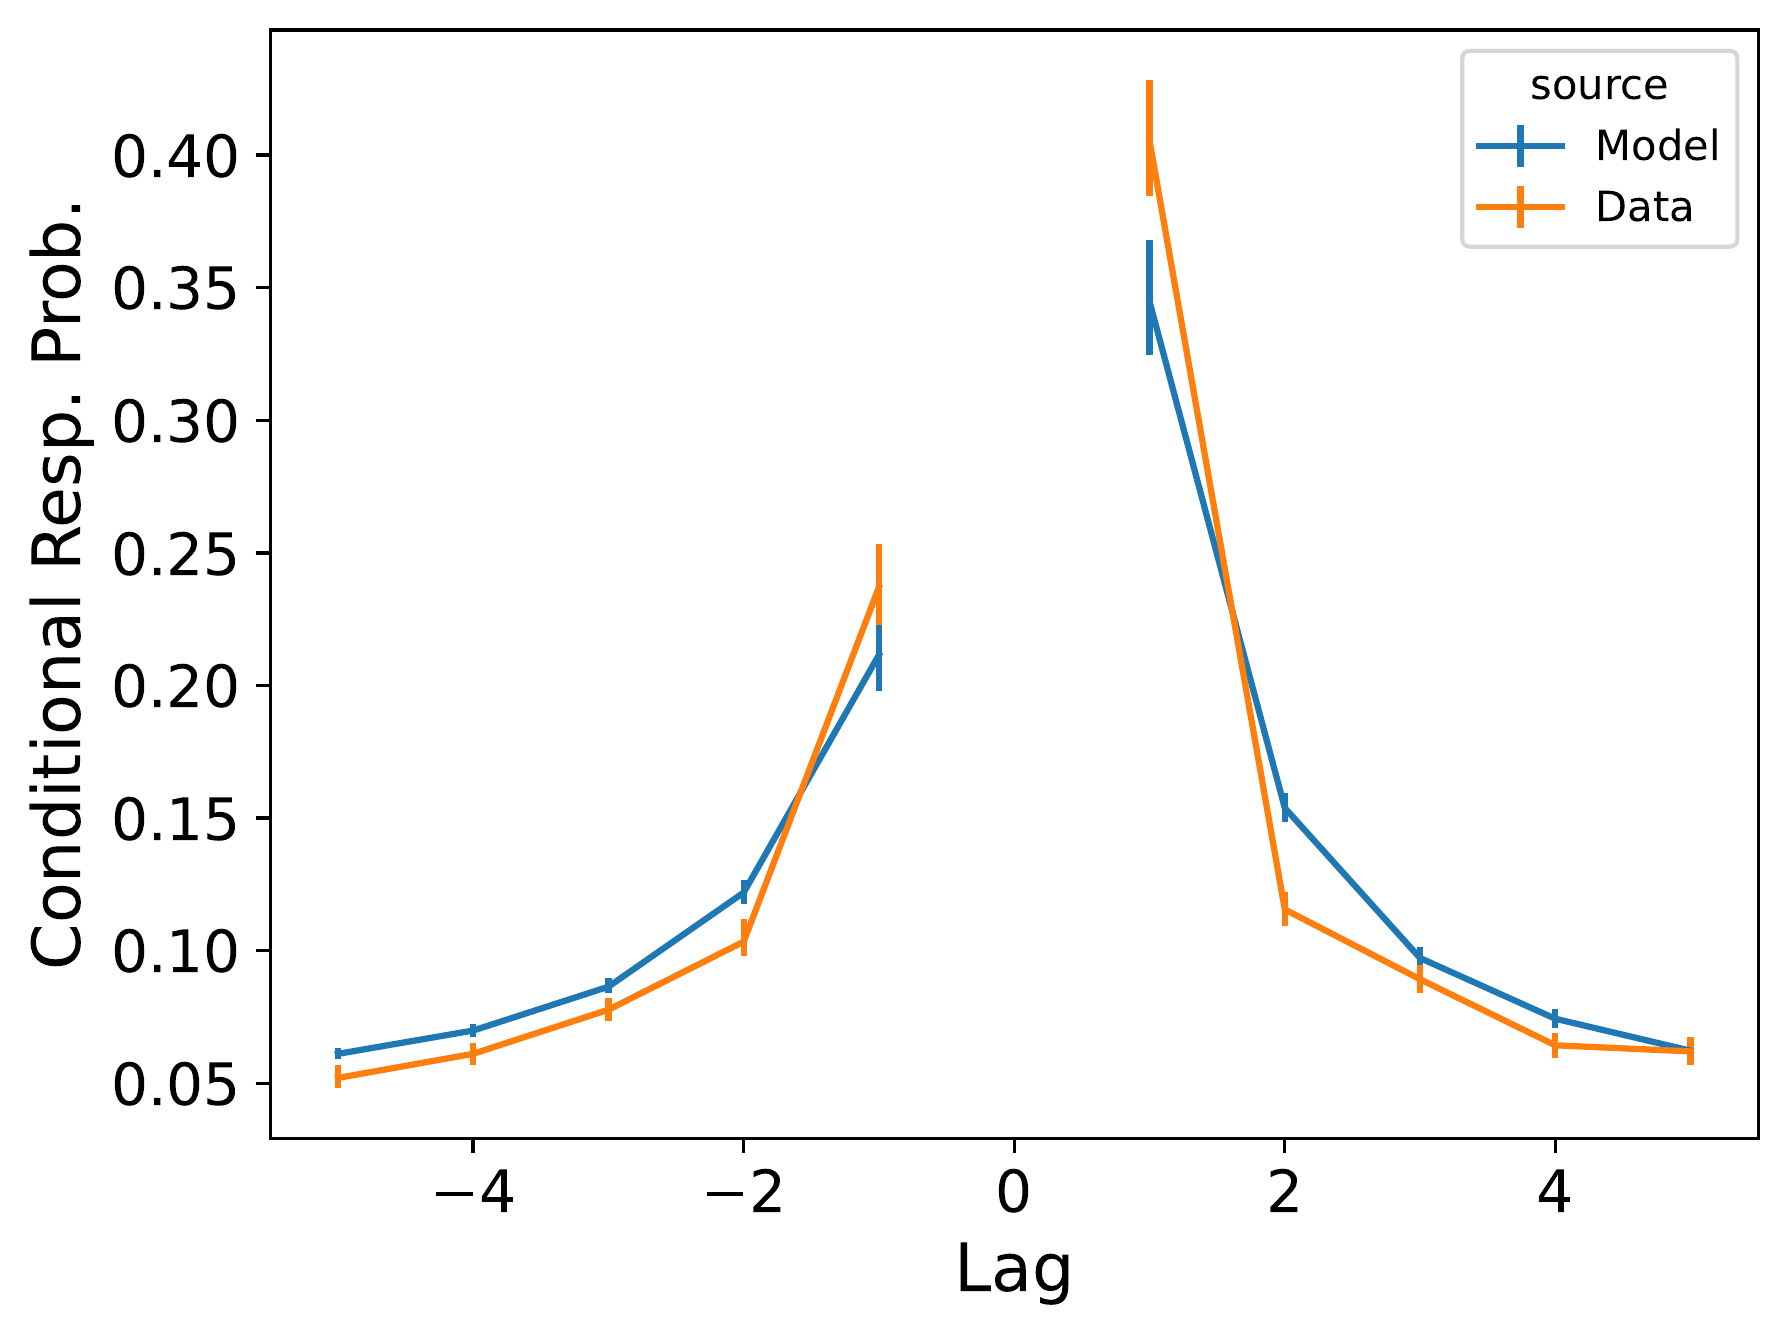
\includegraphics{../../work/thesis/icmr_figures/HealyKahana2014_ConnectionistCMR_Model_Fitting_crp-1.png}
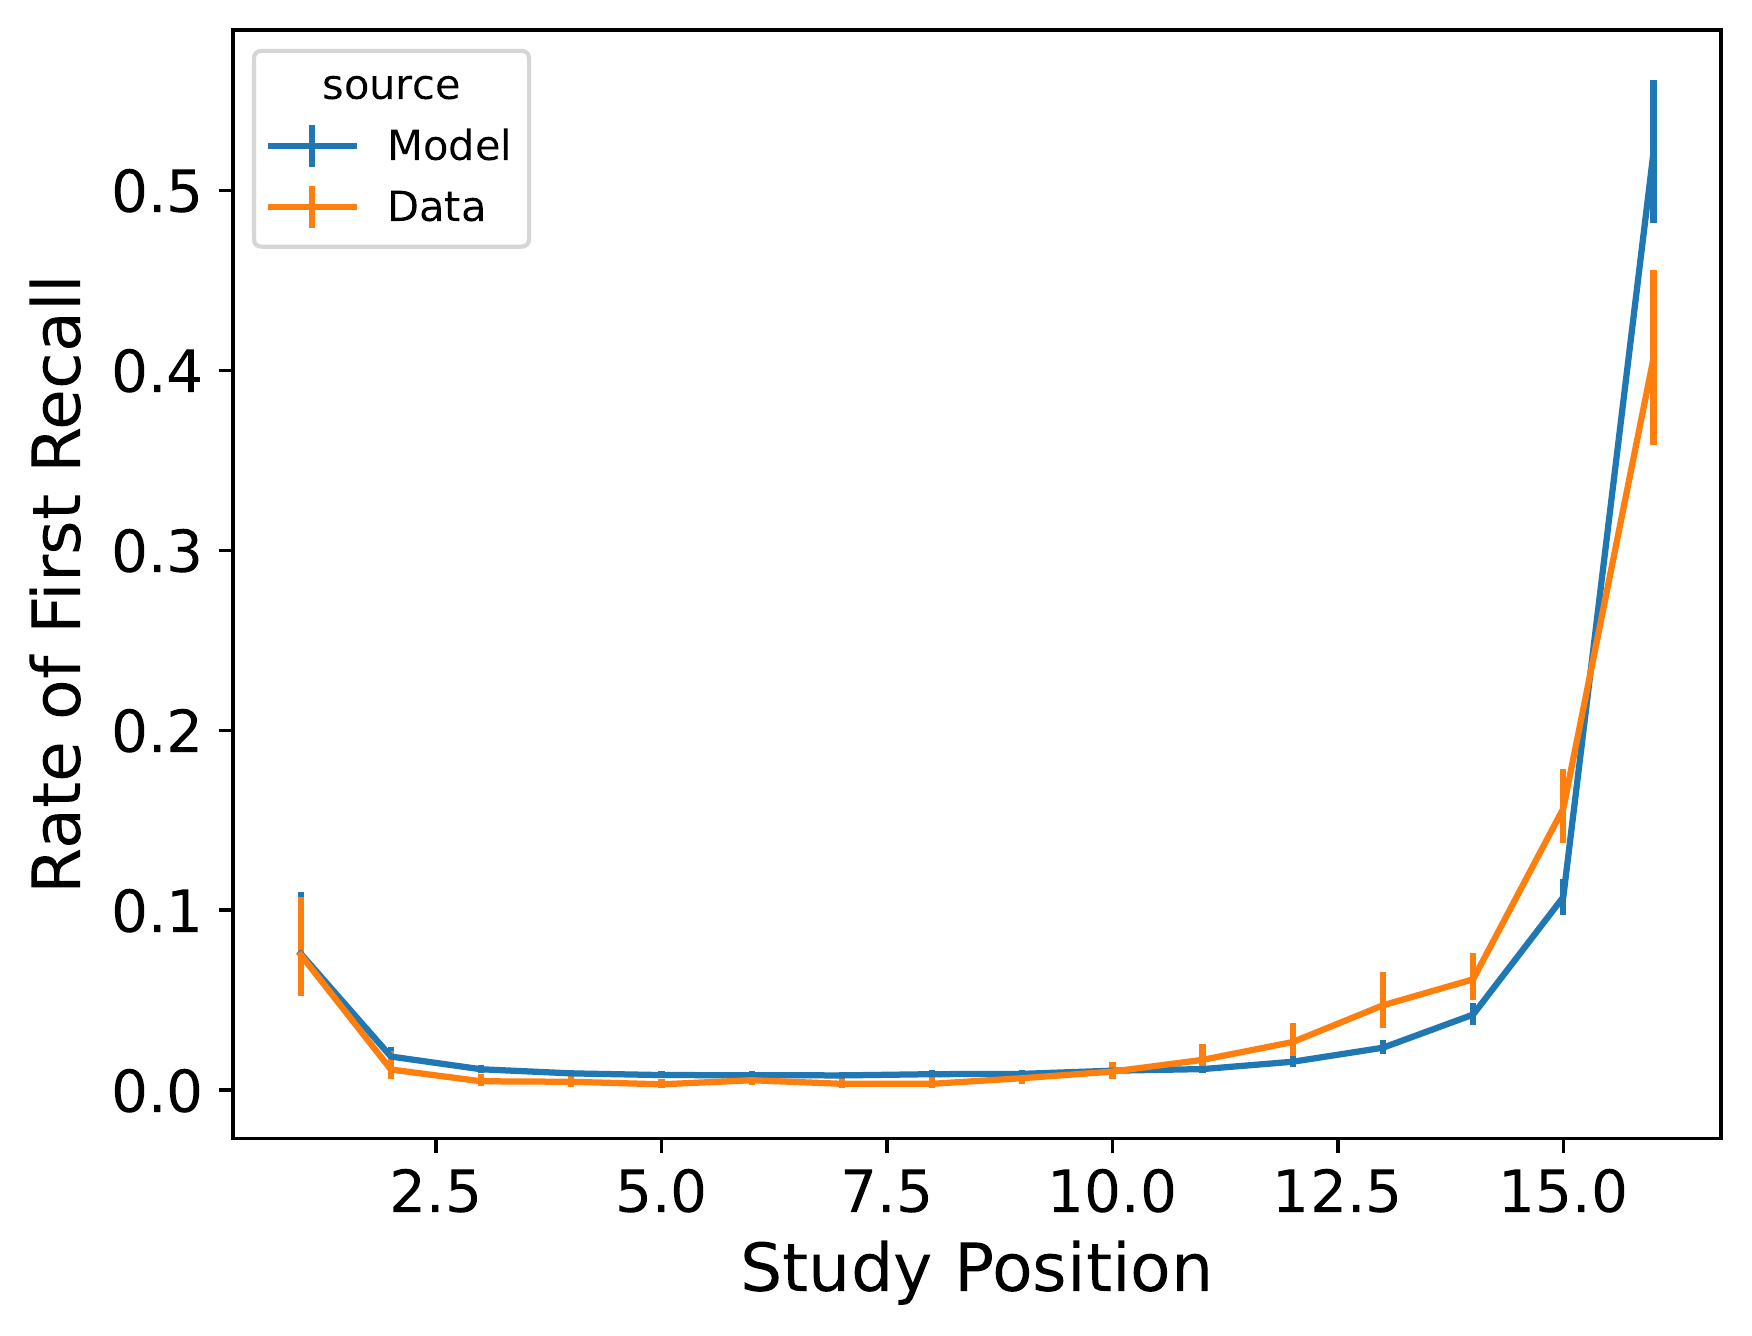
\includegraphics{../../work/thesis/icmr_figures/HealyKahana2014_ConnectionistCMR_Model_Fitting_pfr-1.png}
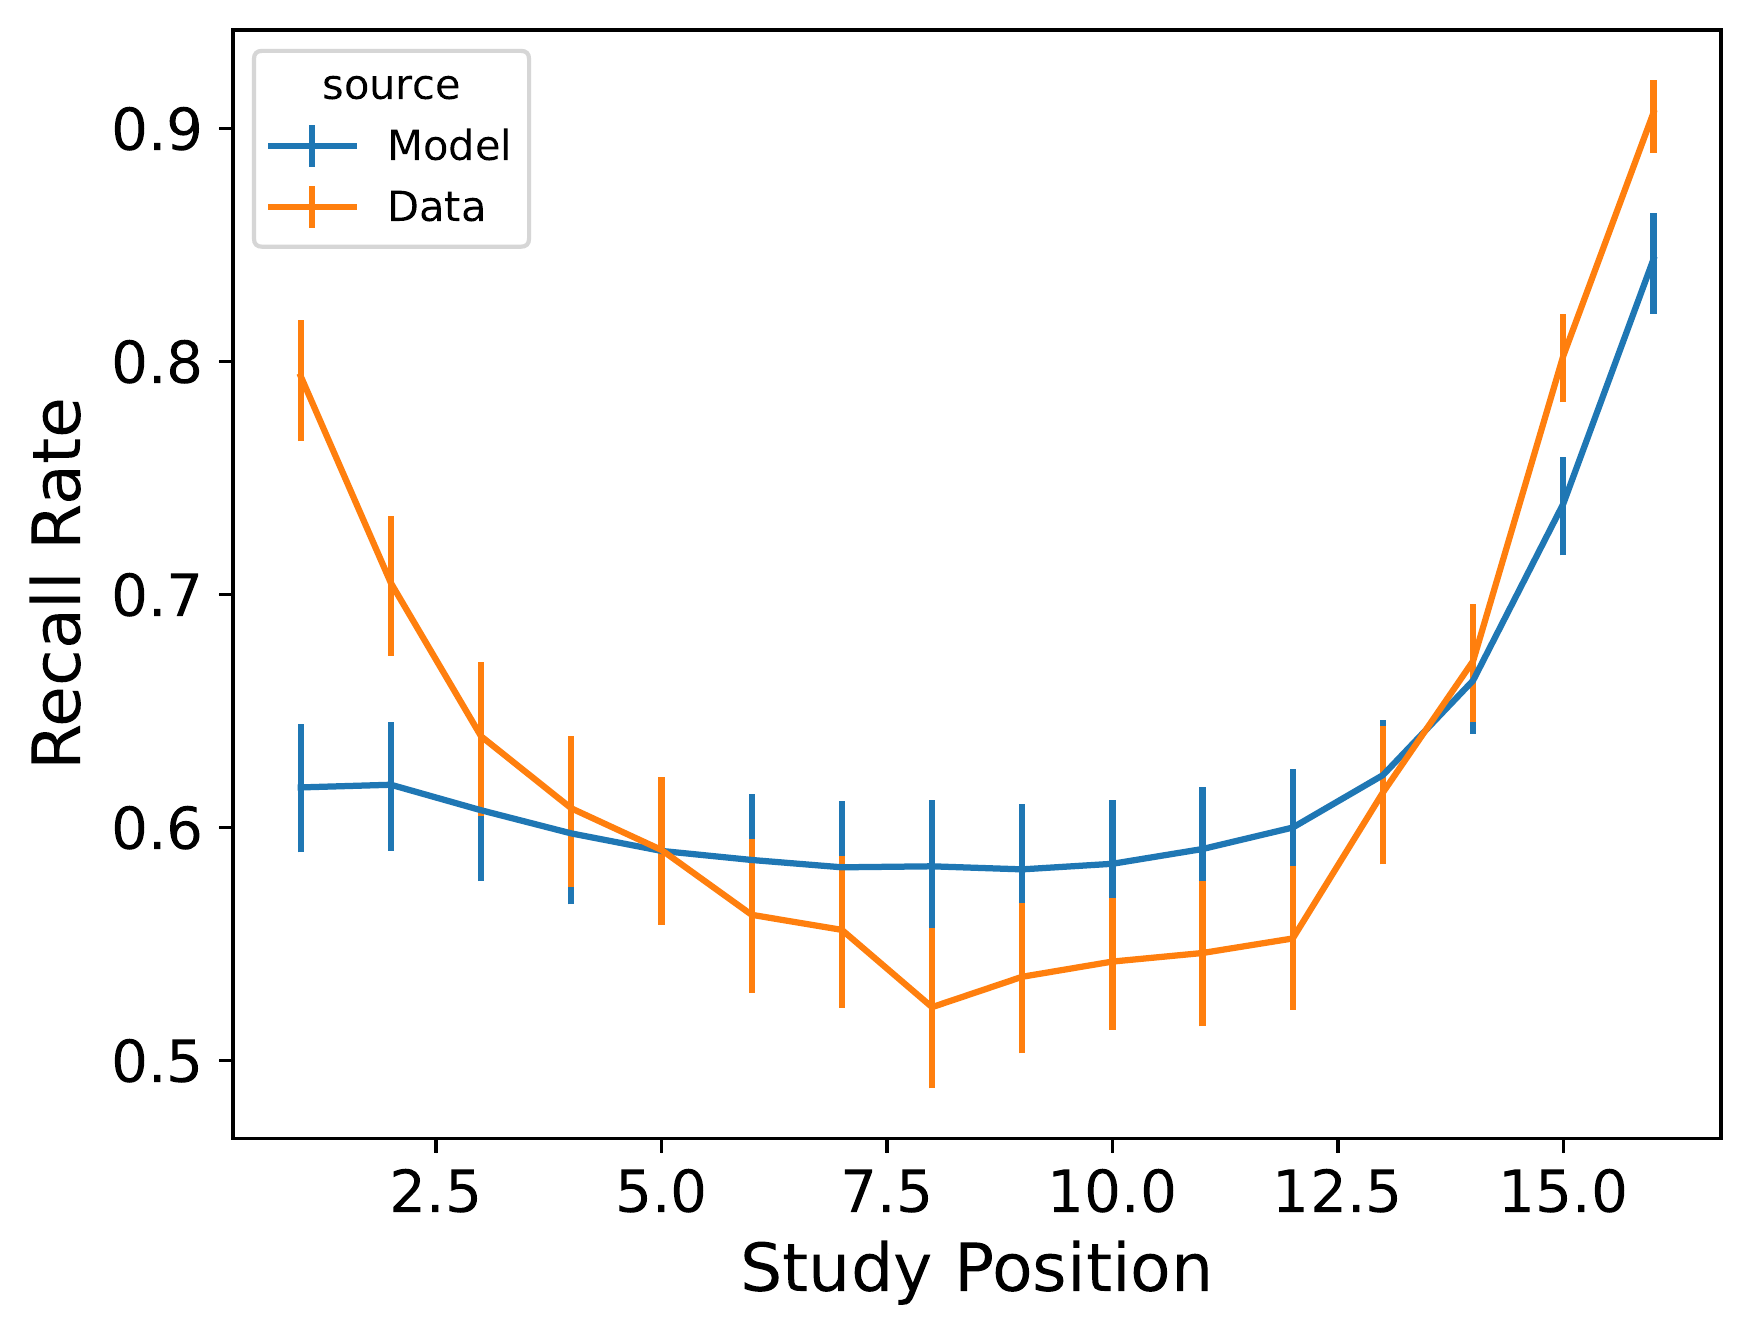
\includegraphics{../../work/thesis/icmr_figures/HealyKahana2014_ConnectionistCMR_Model_Fitting_spc-1.png}\end{minipage}%
%
\begin{minipage}{0.33\linewidth}
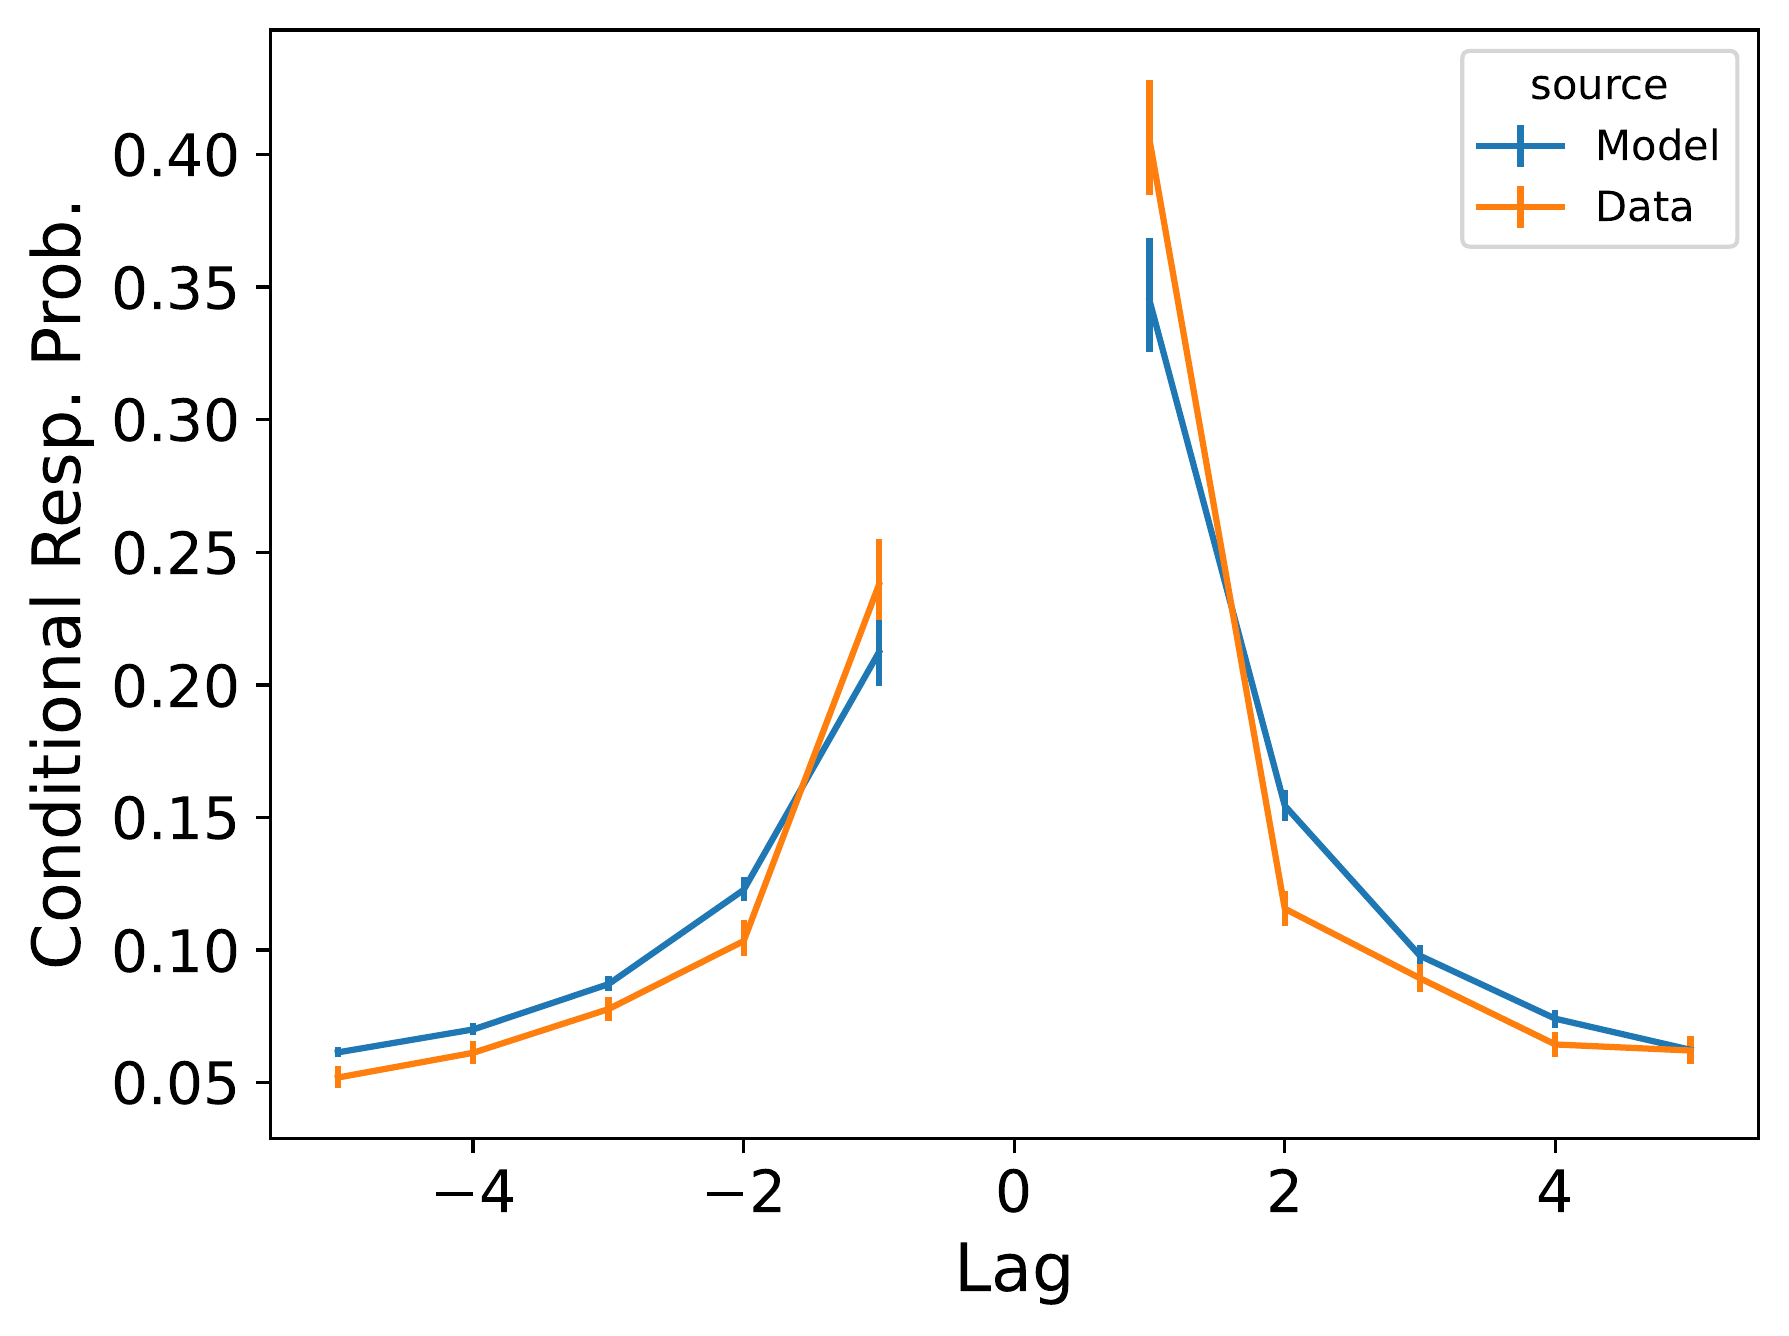
\includegraphics{../../work/thesis/icmr_figures/HealyKahana2014_InstanceCMR_Model_Fitting_crp-1.png}
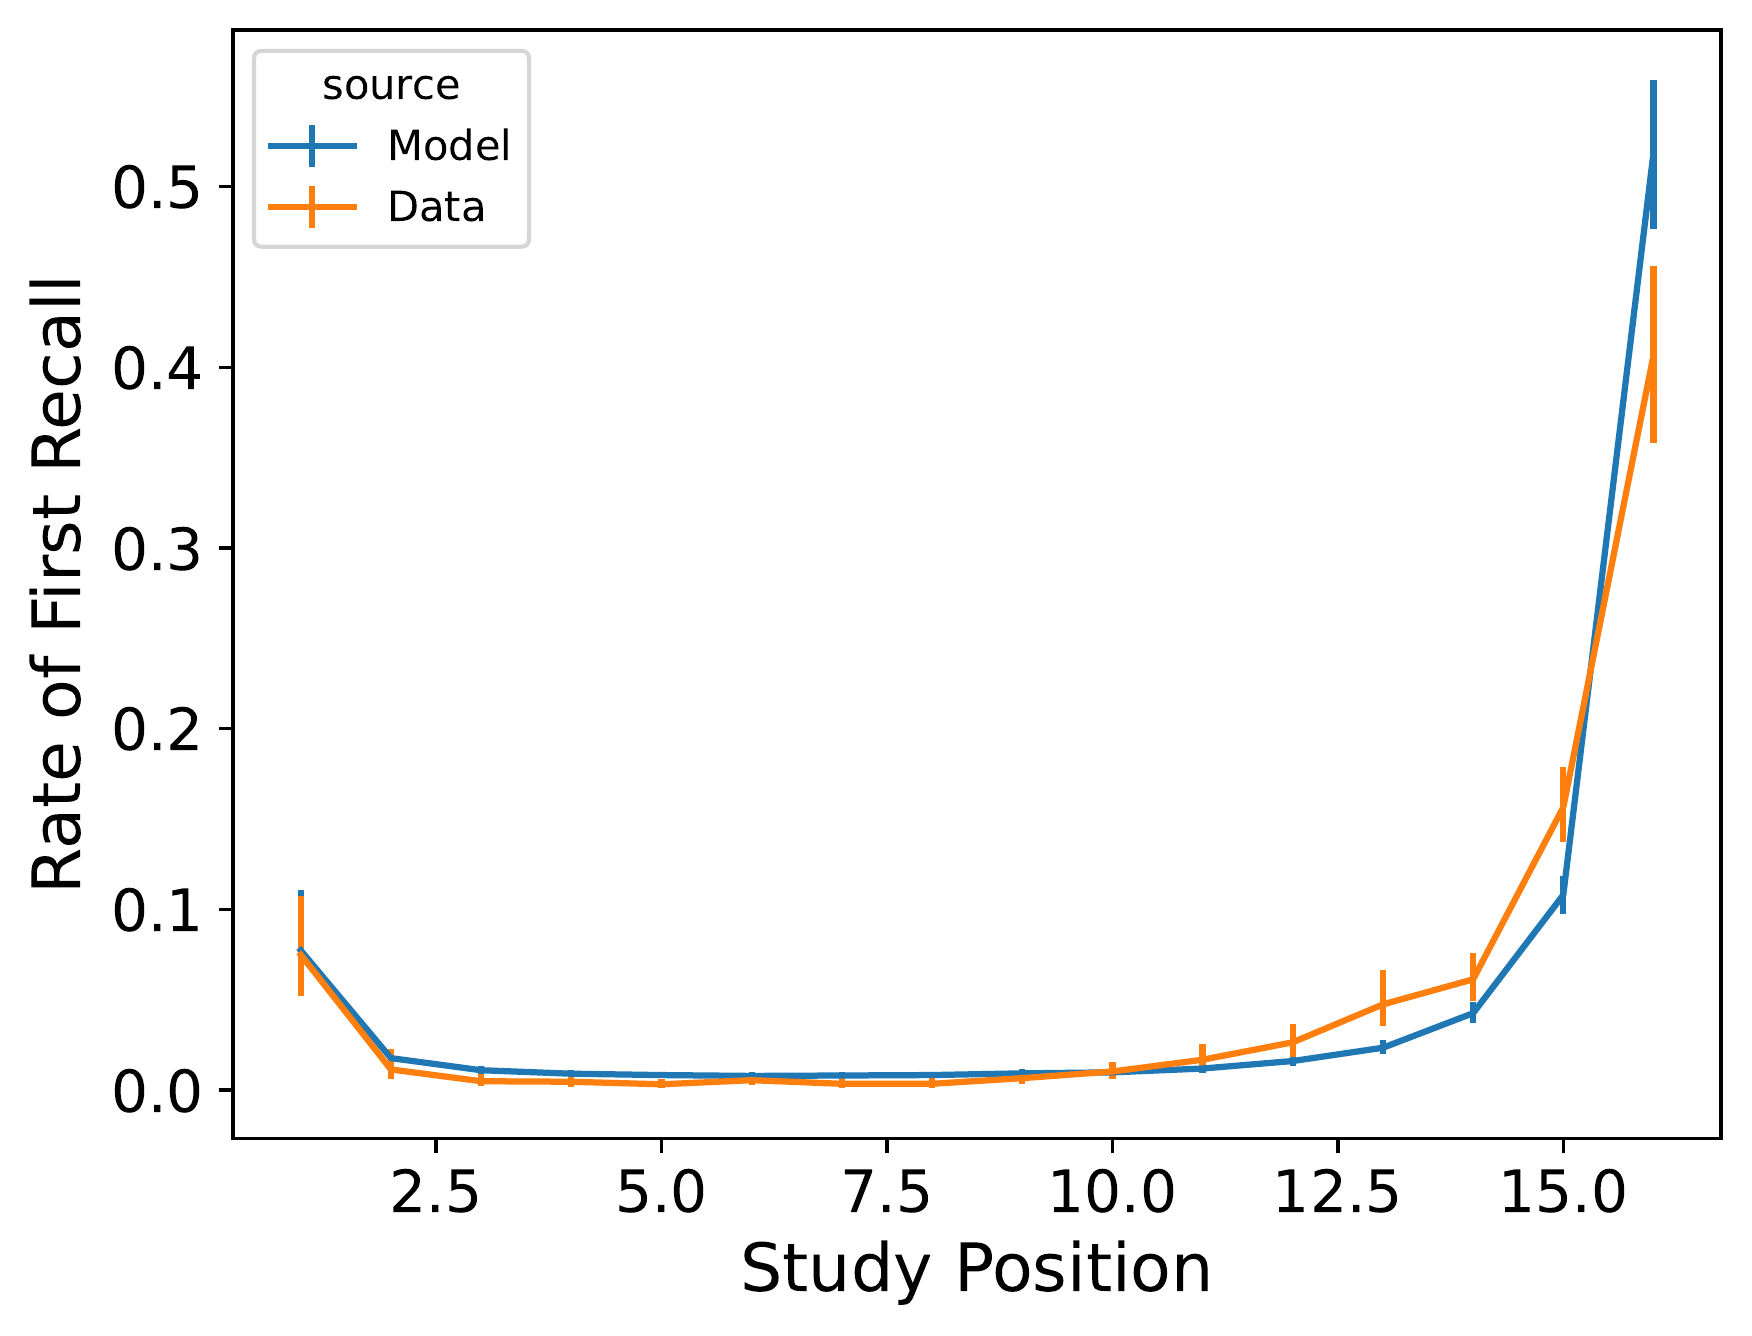
\includegraphics{../../work/thesis/icmr_figures/HealyKahana2014_InstanceCMR_Model_Fitting_pfr-1.png}
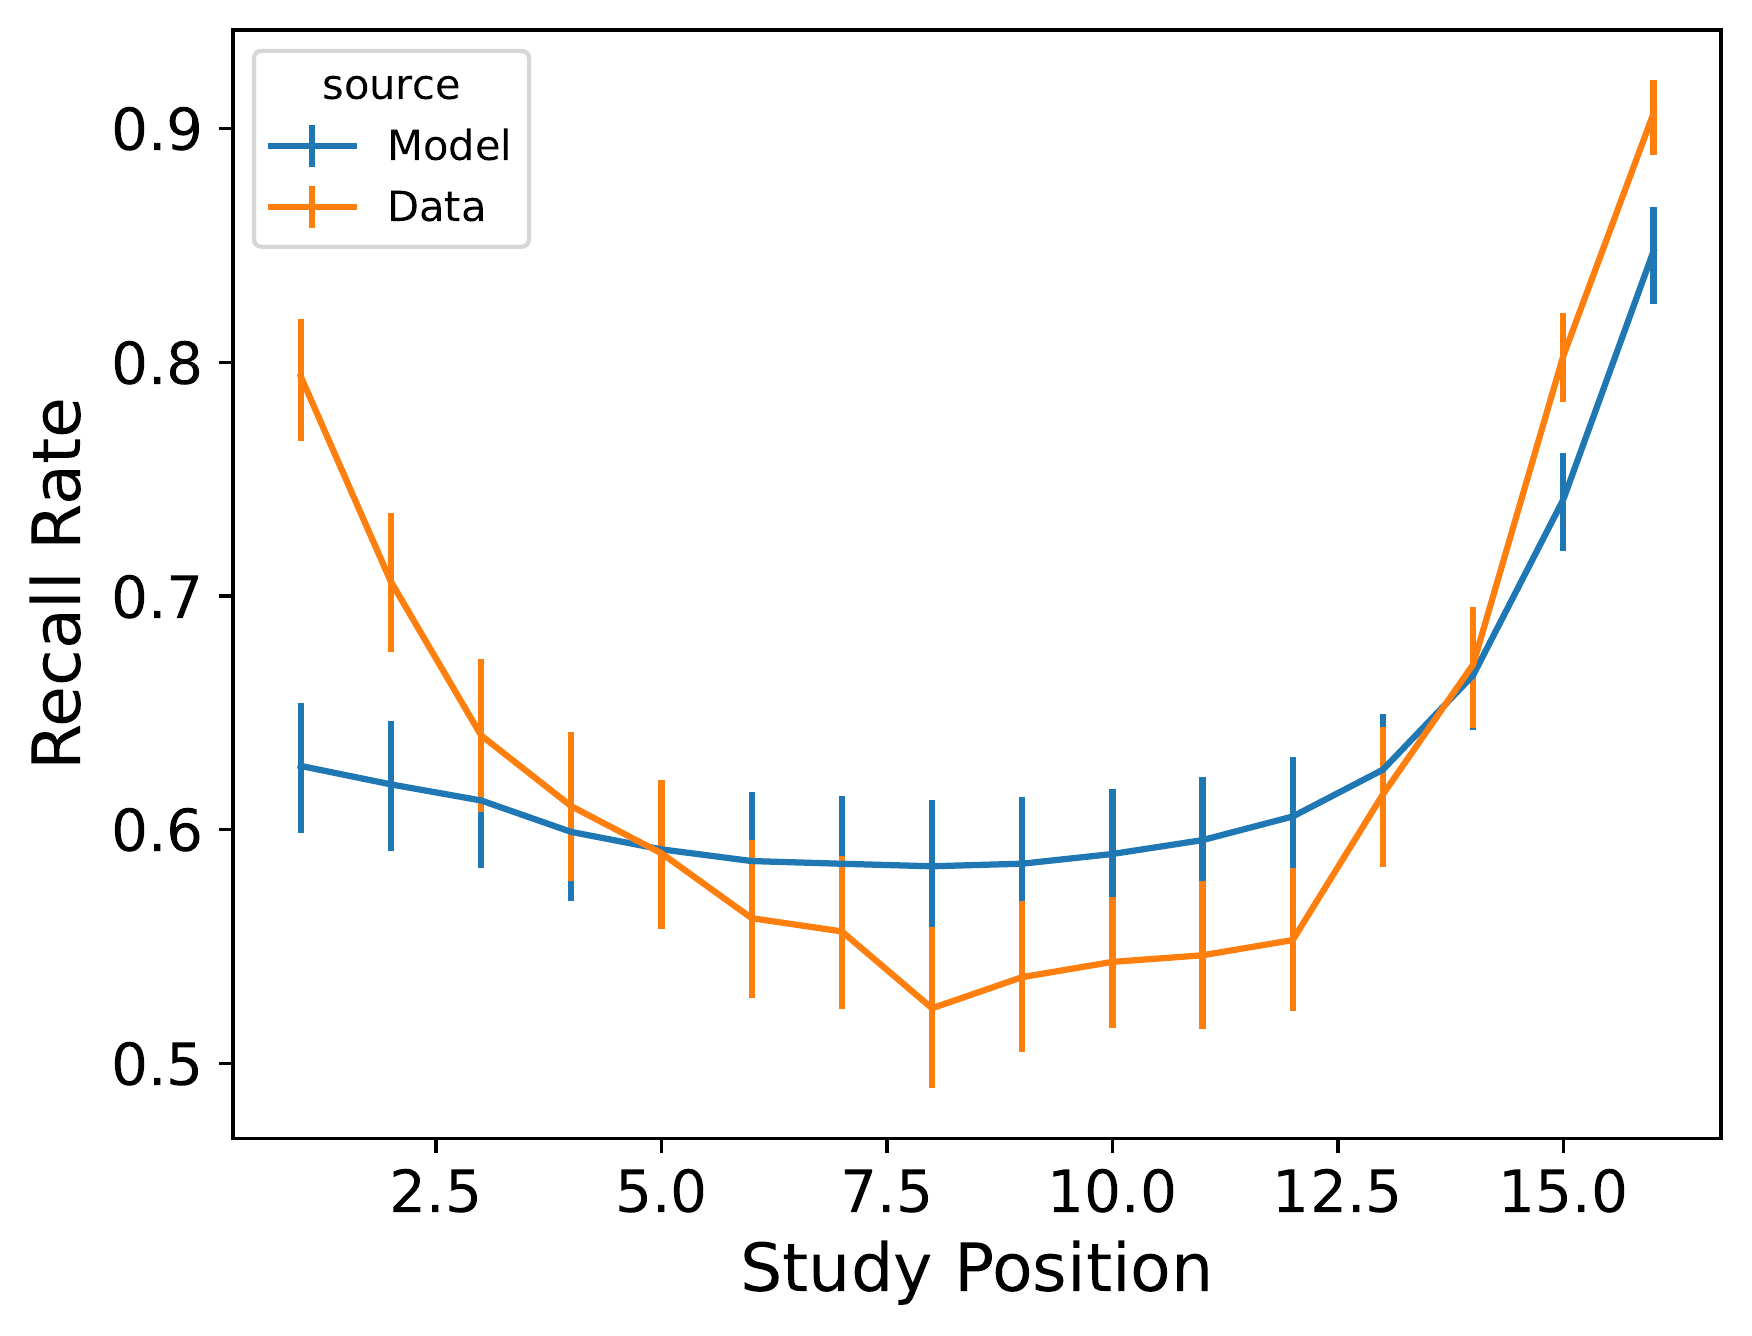
\includegraphics{../../work/thesis/icmr_figures/HealyKahana2014_InstanceCMR_Model_Fitting_spc-1.png}\end{minipage}%

\end{figure}%

\section{Reassessing Empirical Benchmarks Against
CMR}\label{reassessing-empirical-benchmarks-against-cmr}

Before turning to repetition-specific diagnostics, we verify that mixed
and control lists are comparable once the matched, symmetric baseline is
applied, and that standard CMR reproduces the benchmarks that any viable
free-recall account must capture. Error bars for any figure reflect a
bootstrapped 95\% confidence interval over subject means, enabling
statistical inference on the group level.
Figure~\ref{fig-control_method} shows serial-position curves (SPCs),
lag-conditional response probabilities (lag-CRPs), and probabilities of
first recall (PFRs) for mixed and control lists in Lohnas and Kahana
(\citeproc{ref-lohnas2014retrieved}{2014}), plotted in raw form (left)
and after baseline correction (right). In the raw SPCs, mixed lists
appear to enjoy a mid-list advantage; after position matching and
symmetric scoring this inflation vanishes, and SPCs from mixed and
control lists are essentially indistinguishable. Small raw differences
in the lag-CRP likewise disappear under the baseline, and the PFRs are
virtually identical across conditions. With the basic benchmarks
satisfied and no substantive differences between mixed and control lists
once the baseline is applied, we can focus on analyses that more
directly test the predictions of item-based context evolution.

Standard CMR broadly reproduces these benchmarks under the same scoring
and similarly predicts limited differences between SPC, PFR, and lag-CRP
outcomes across mixed and control
lists(Figure~\ref{fig-cmr_benchmarks}). We therefore focus our
evaluation on the specific predictions that arise from the model's
treatment of repeated items.

\begin{figure}

\caption{\label{fig-control_method}Raw (Left) vs control-corrected
(Right) benchmark summary statistics for mixed vs control list trials
from Lohnas and Kahana (\citeproc{ref-lohnas2014retrieved}{2014}). Top
row: recall rate by serial position (serial position curve, SPC). Second
row: conditional response probability (CRP) by lag. Third row:
probability of first recall by serial position.}

\begin{minipage}{0.50\linewidth}
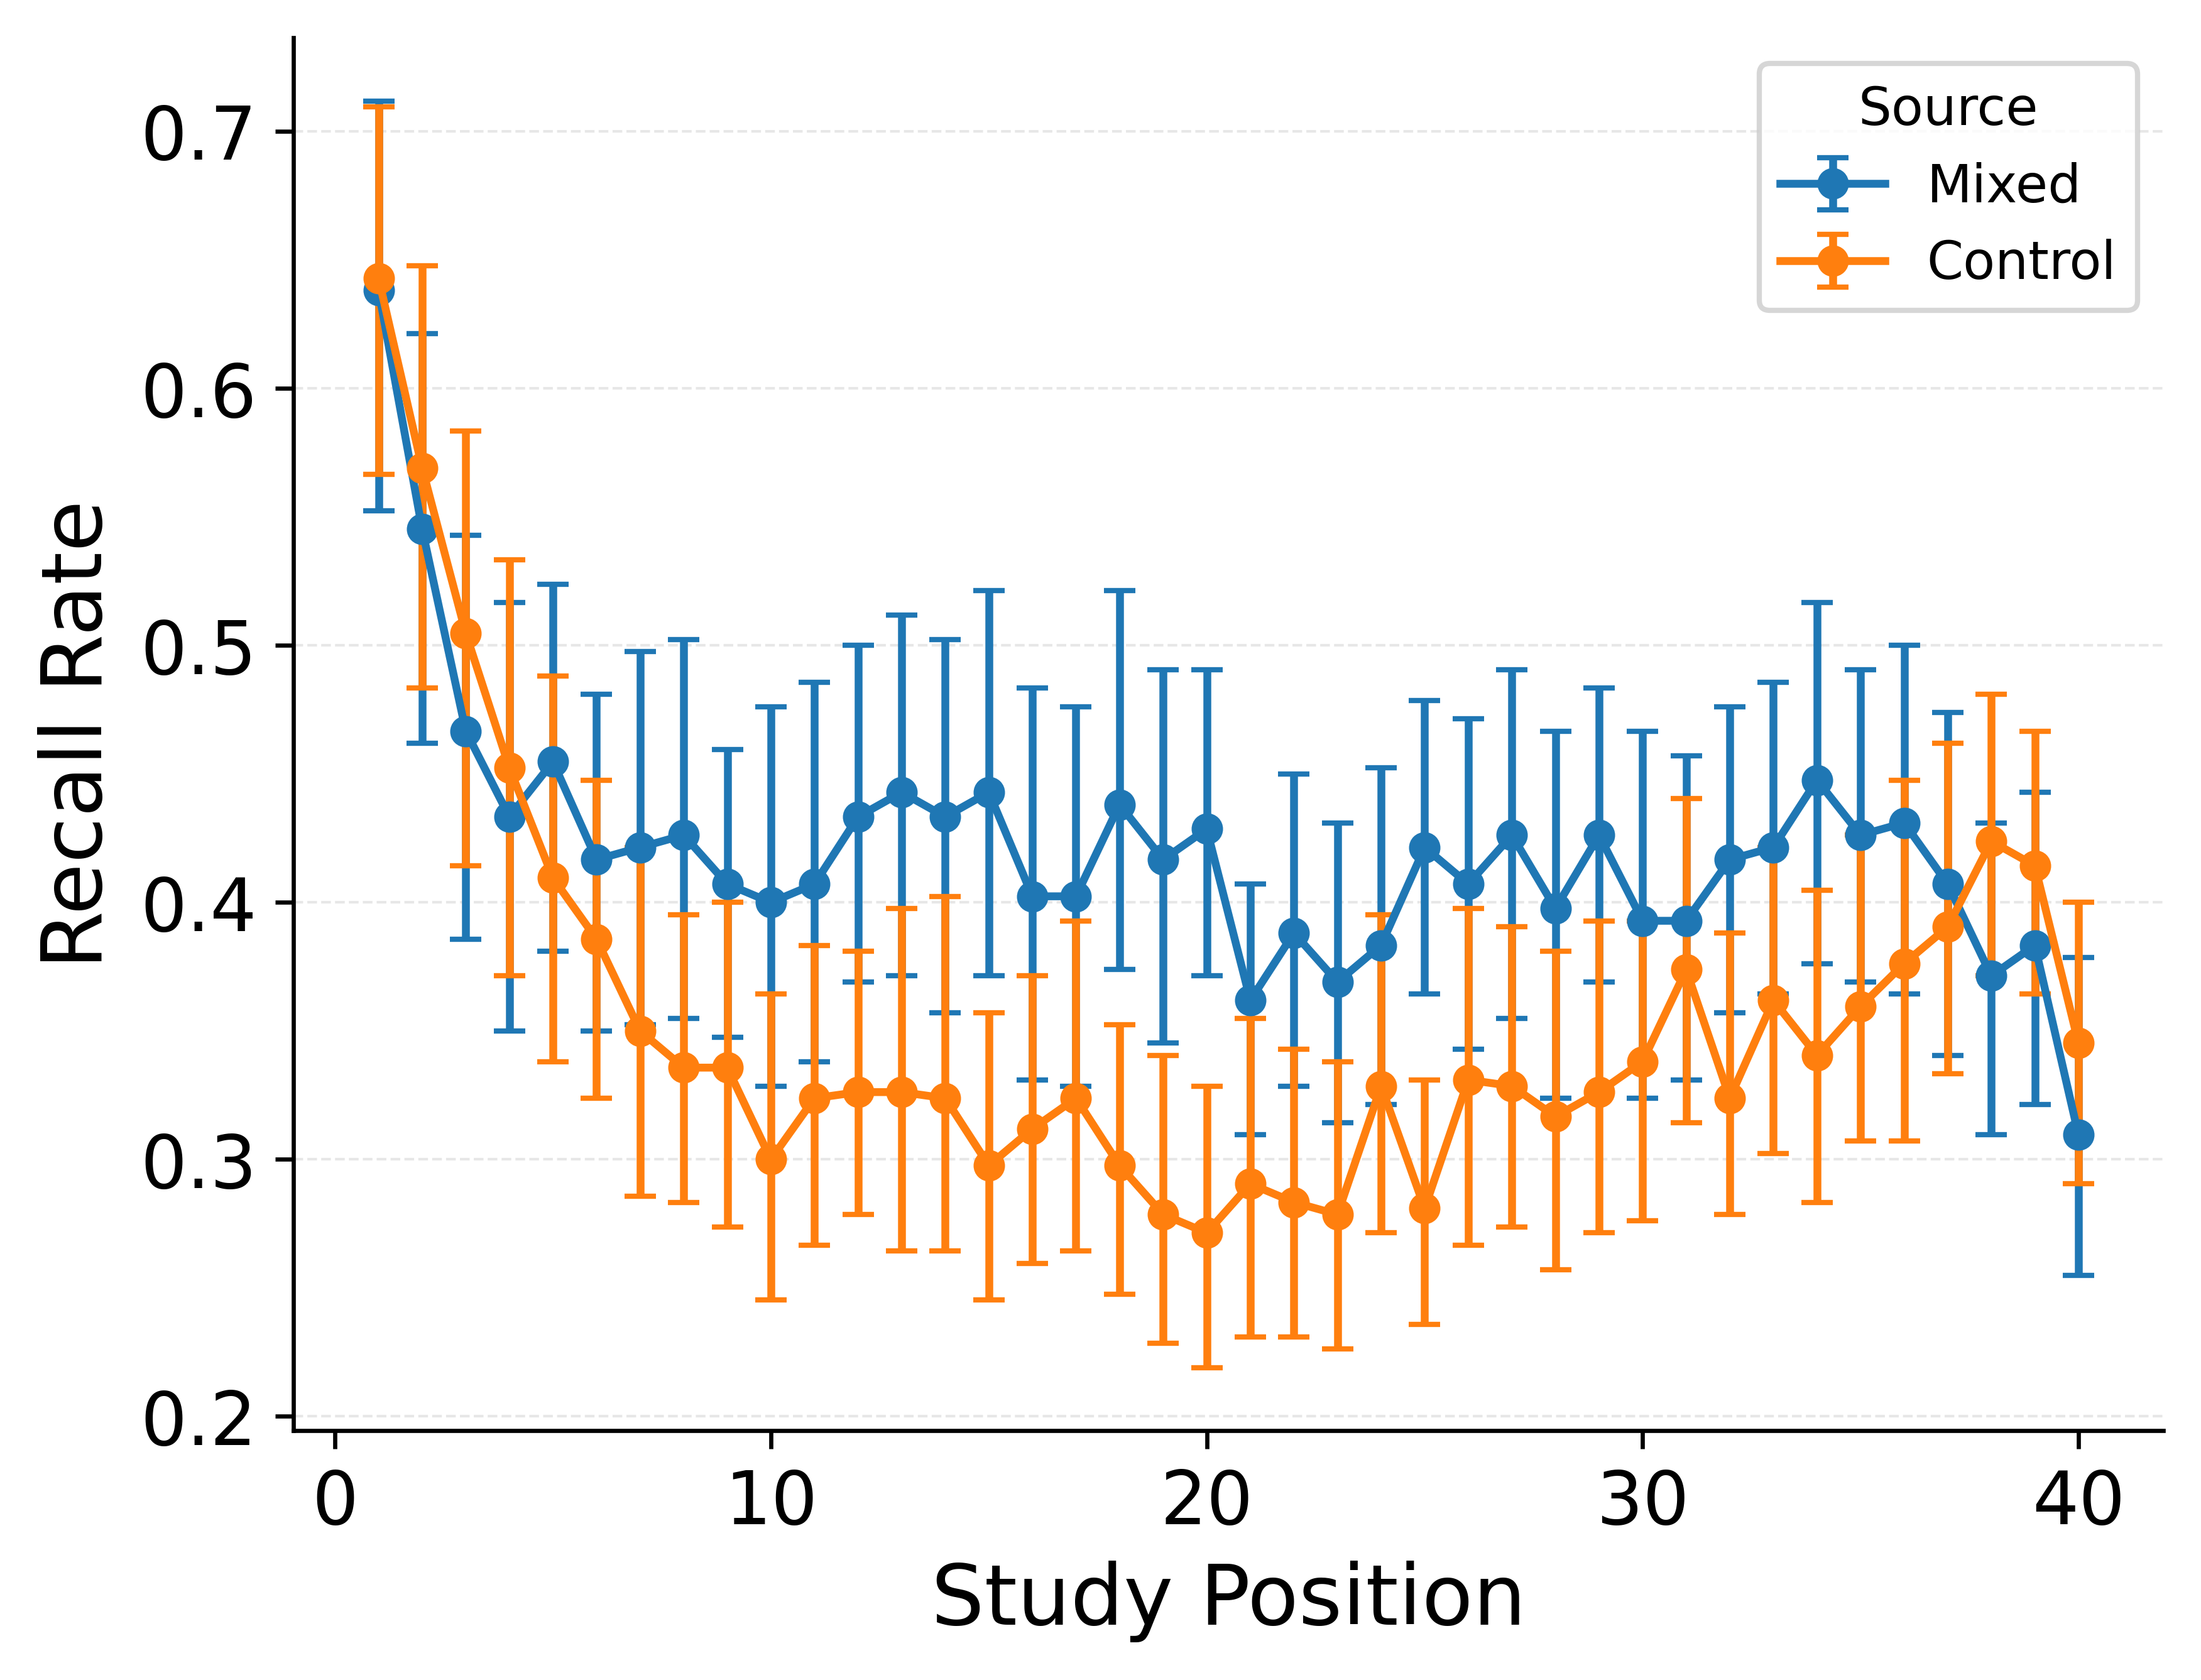
\includegraphics{../../work/thesis/figures/LohnasKahana2014_mixedvscontrolB_data_full_best_of_3_LT4_spc.png}\end{minipage}%
%
\begin{minipage}{0.50\linewidth}
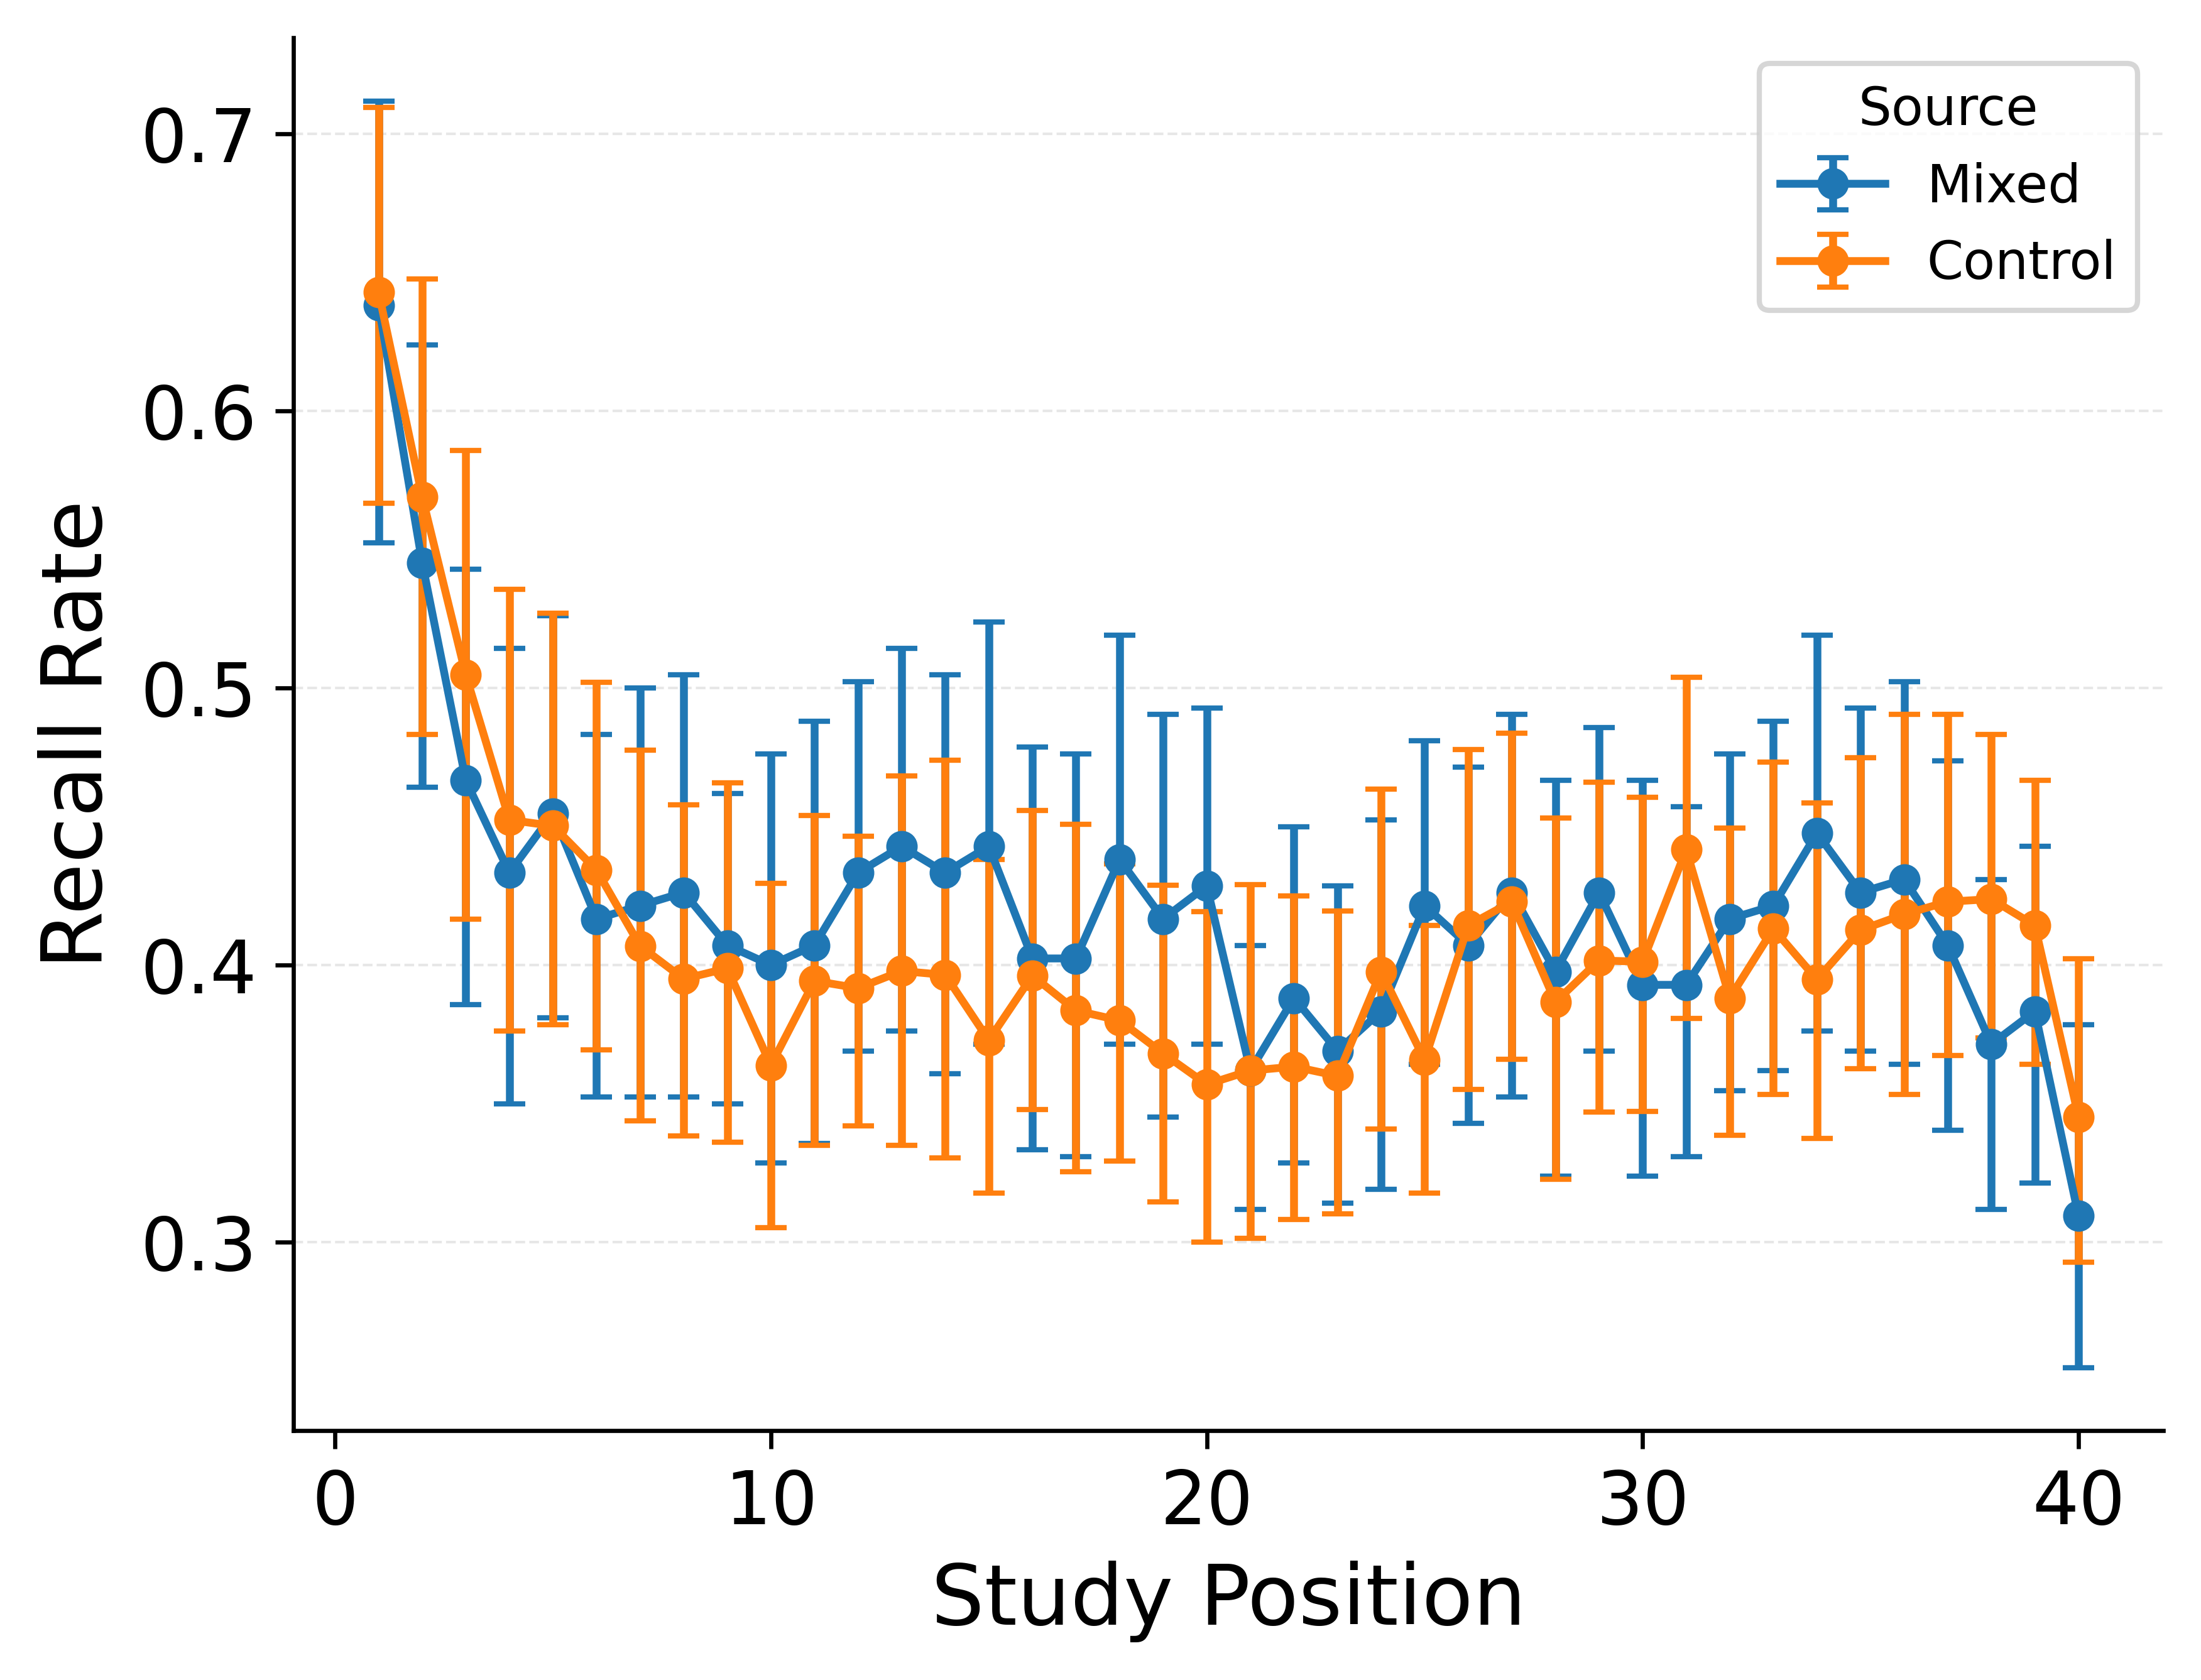
\includegraphics{../../work/thesis/figures/LohnasKahana2014_mixedvscontrolA_data_full_best_of_3_LT4_spc.png}\end{minipage}%
\newline
\begin{minipage}{0.50\linewidth}
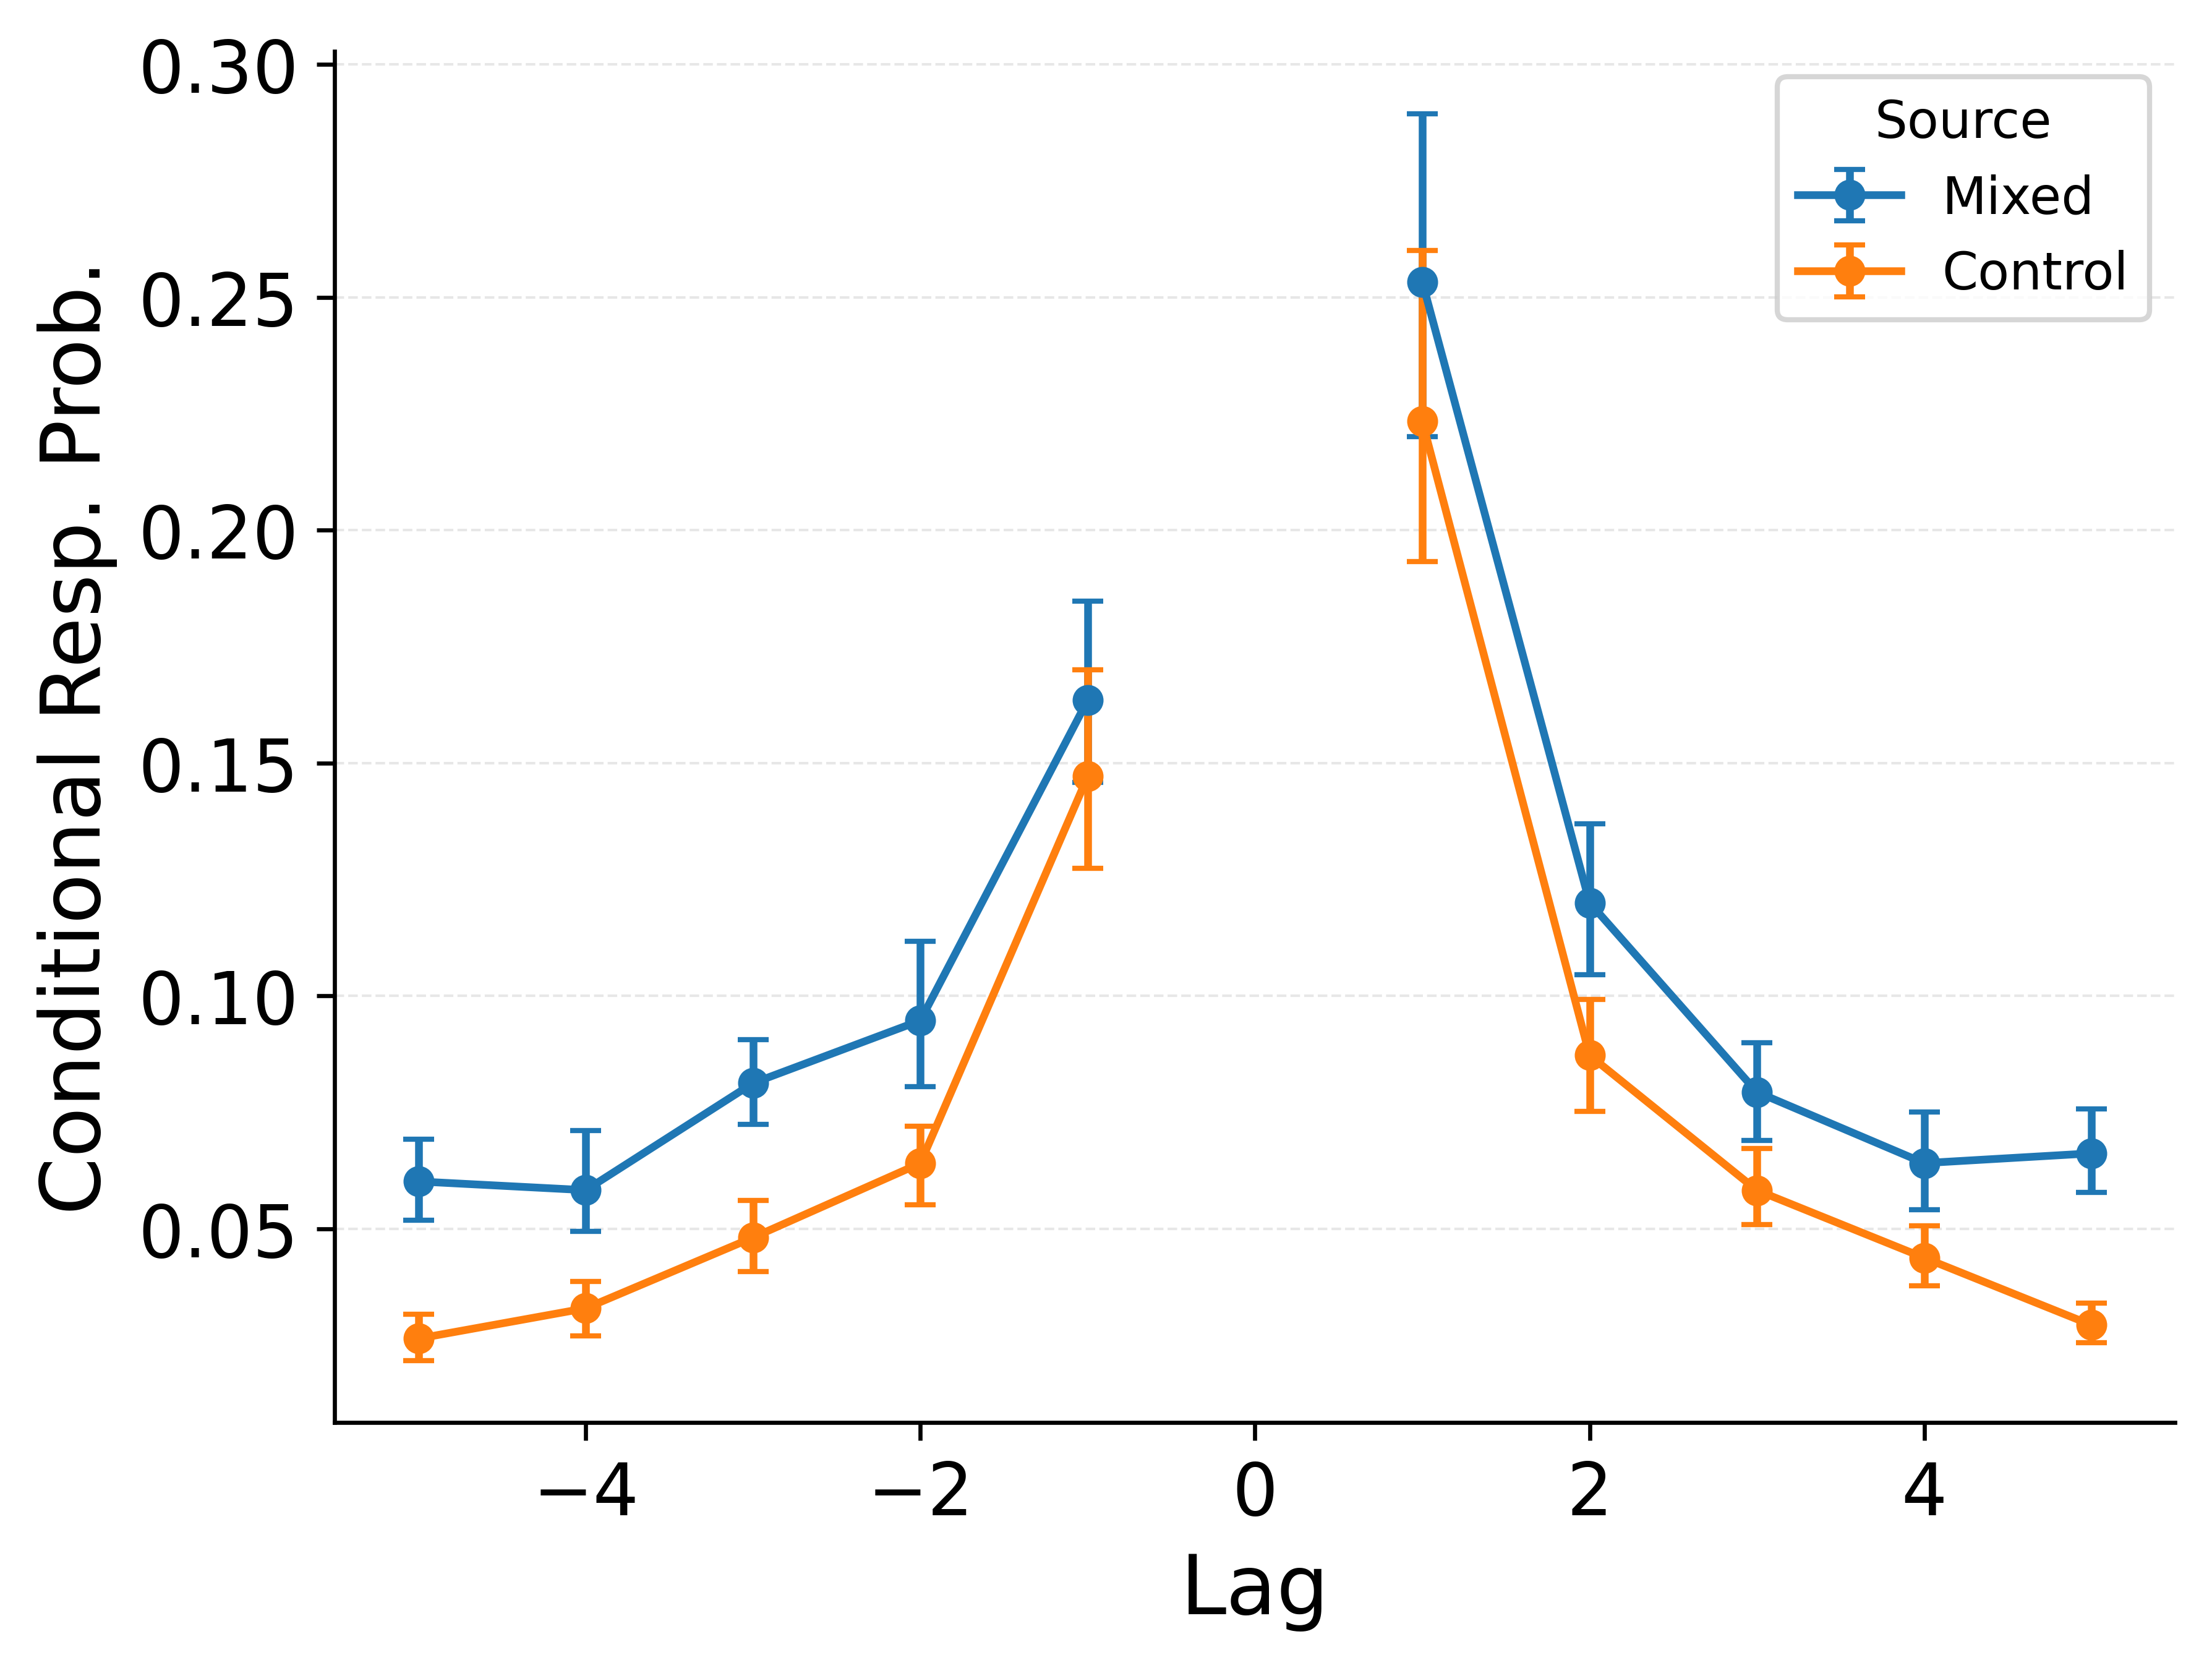
\includegraphics{../../work/thesis/figures/LohnasKahana2014_mixedvscontrolB_data_full_best_of_3_LT4_crp.png}\end{minipage}%
%
\begin{minipage}{0.50\linewidth}
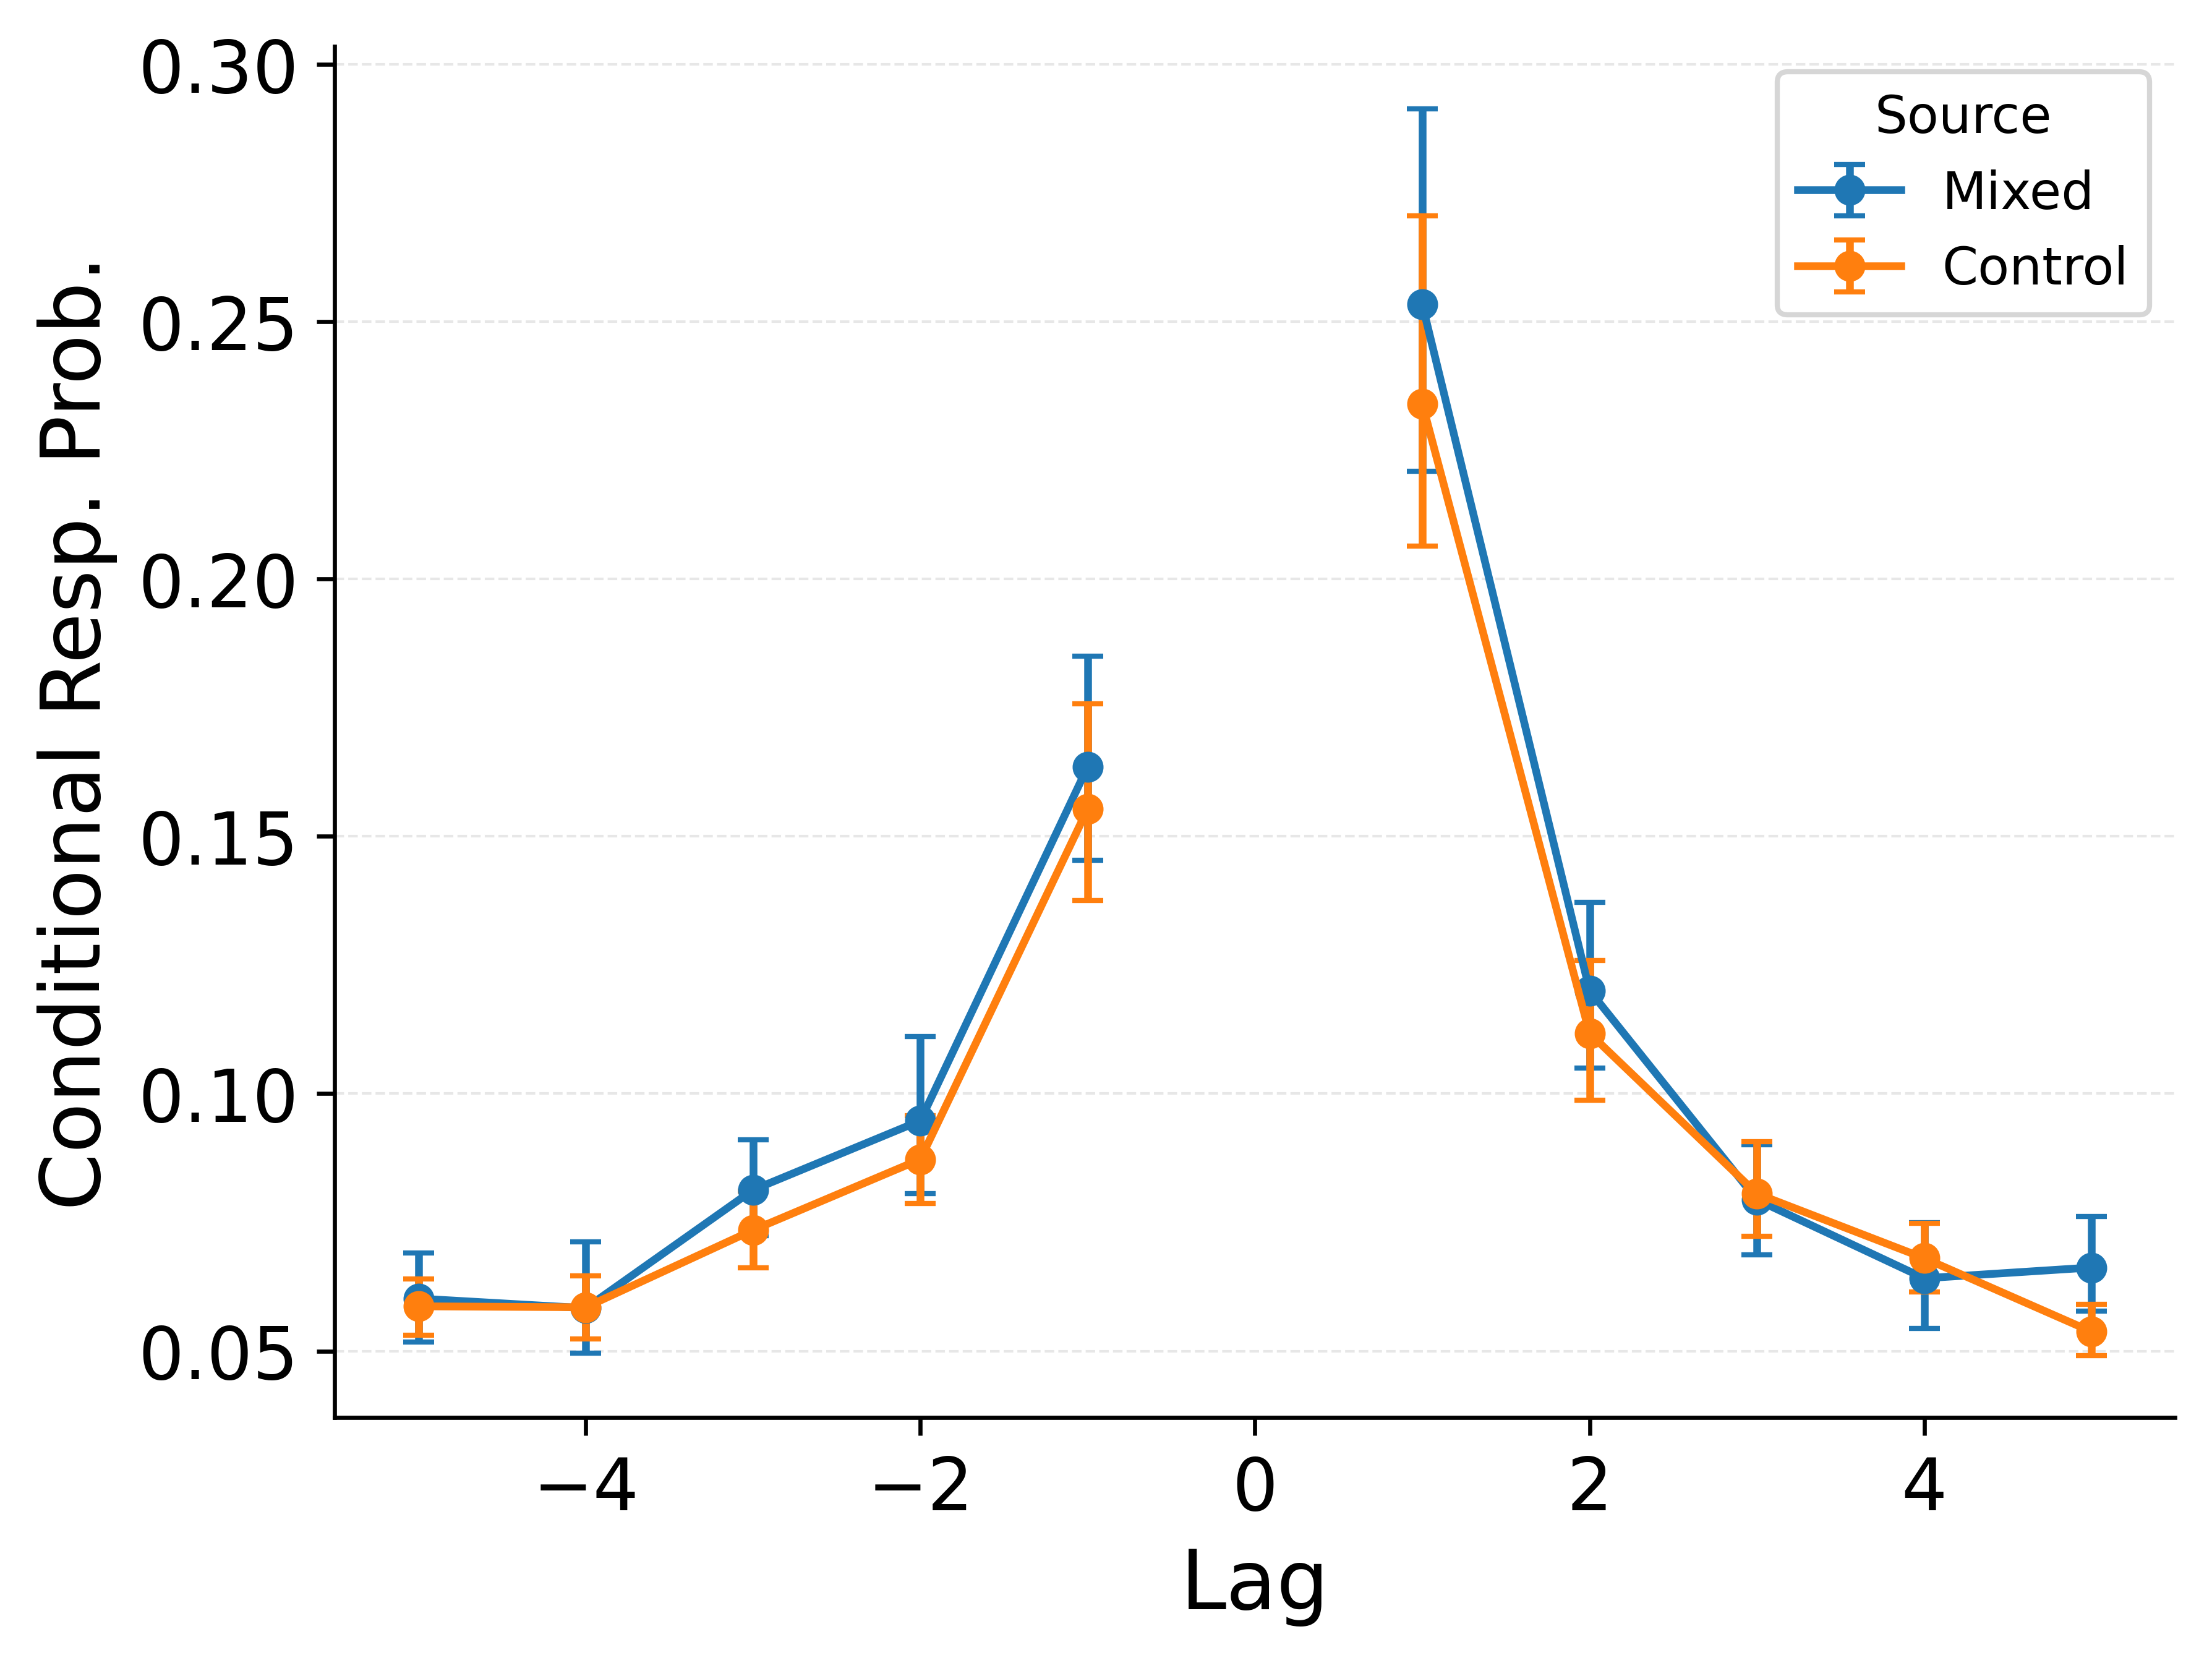
\includegraphics{../../work/thesis/figures/LohnasKahana2014_mixedvscontrolA_data_full_best_of_3_LT4_crp.png}\end{minipage}%
\newline
\begin{minipage}{0.50\linewidth}
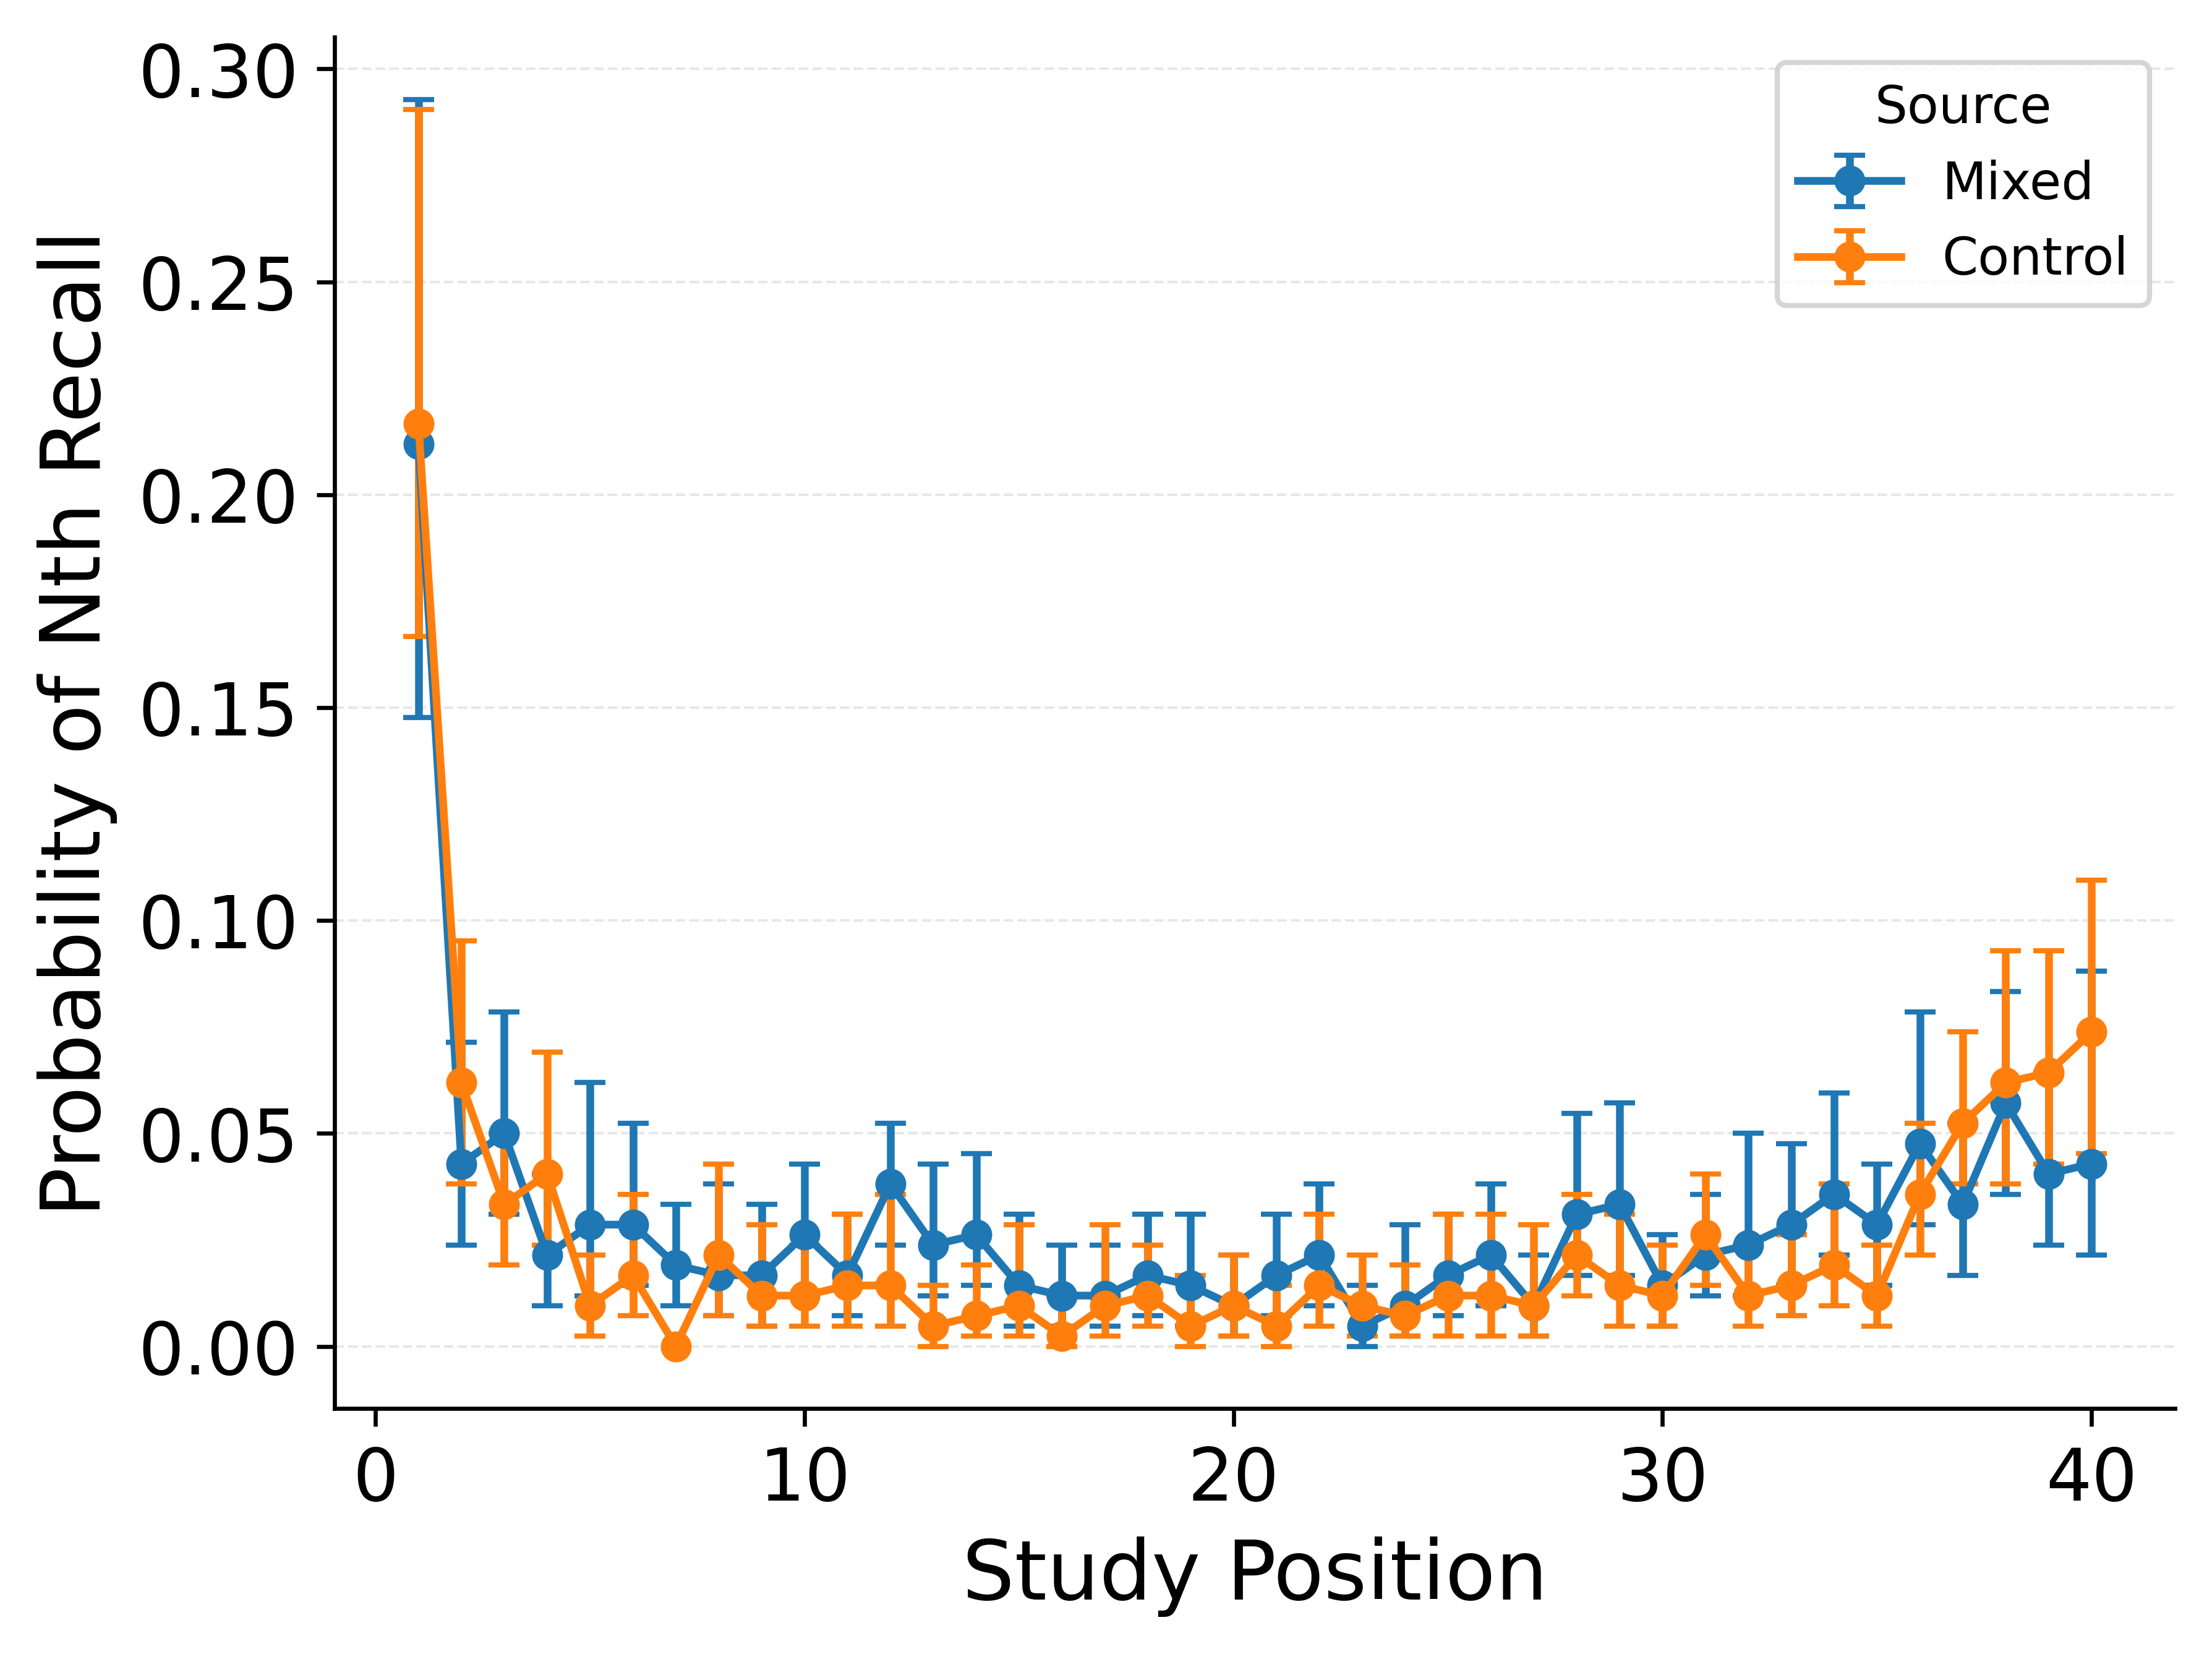
\includegraphics{../../work/thesis/figures/LohnasKahana2014_mixedvscontrolB_data_full_best_of_3_LT4_pnr.png}\end{minipage}%
%
\begin{minipage}{0.50\linewidth}
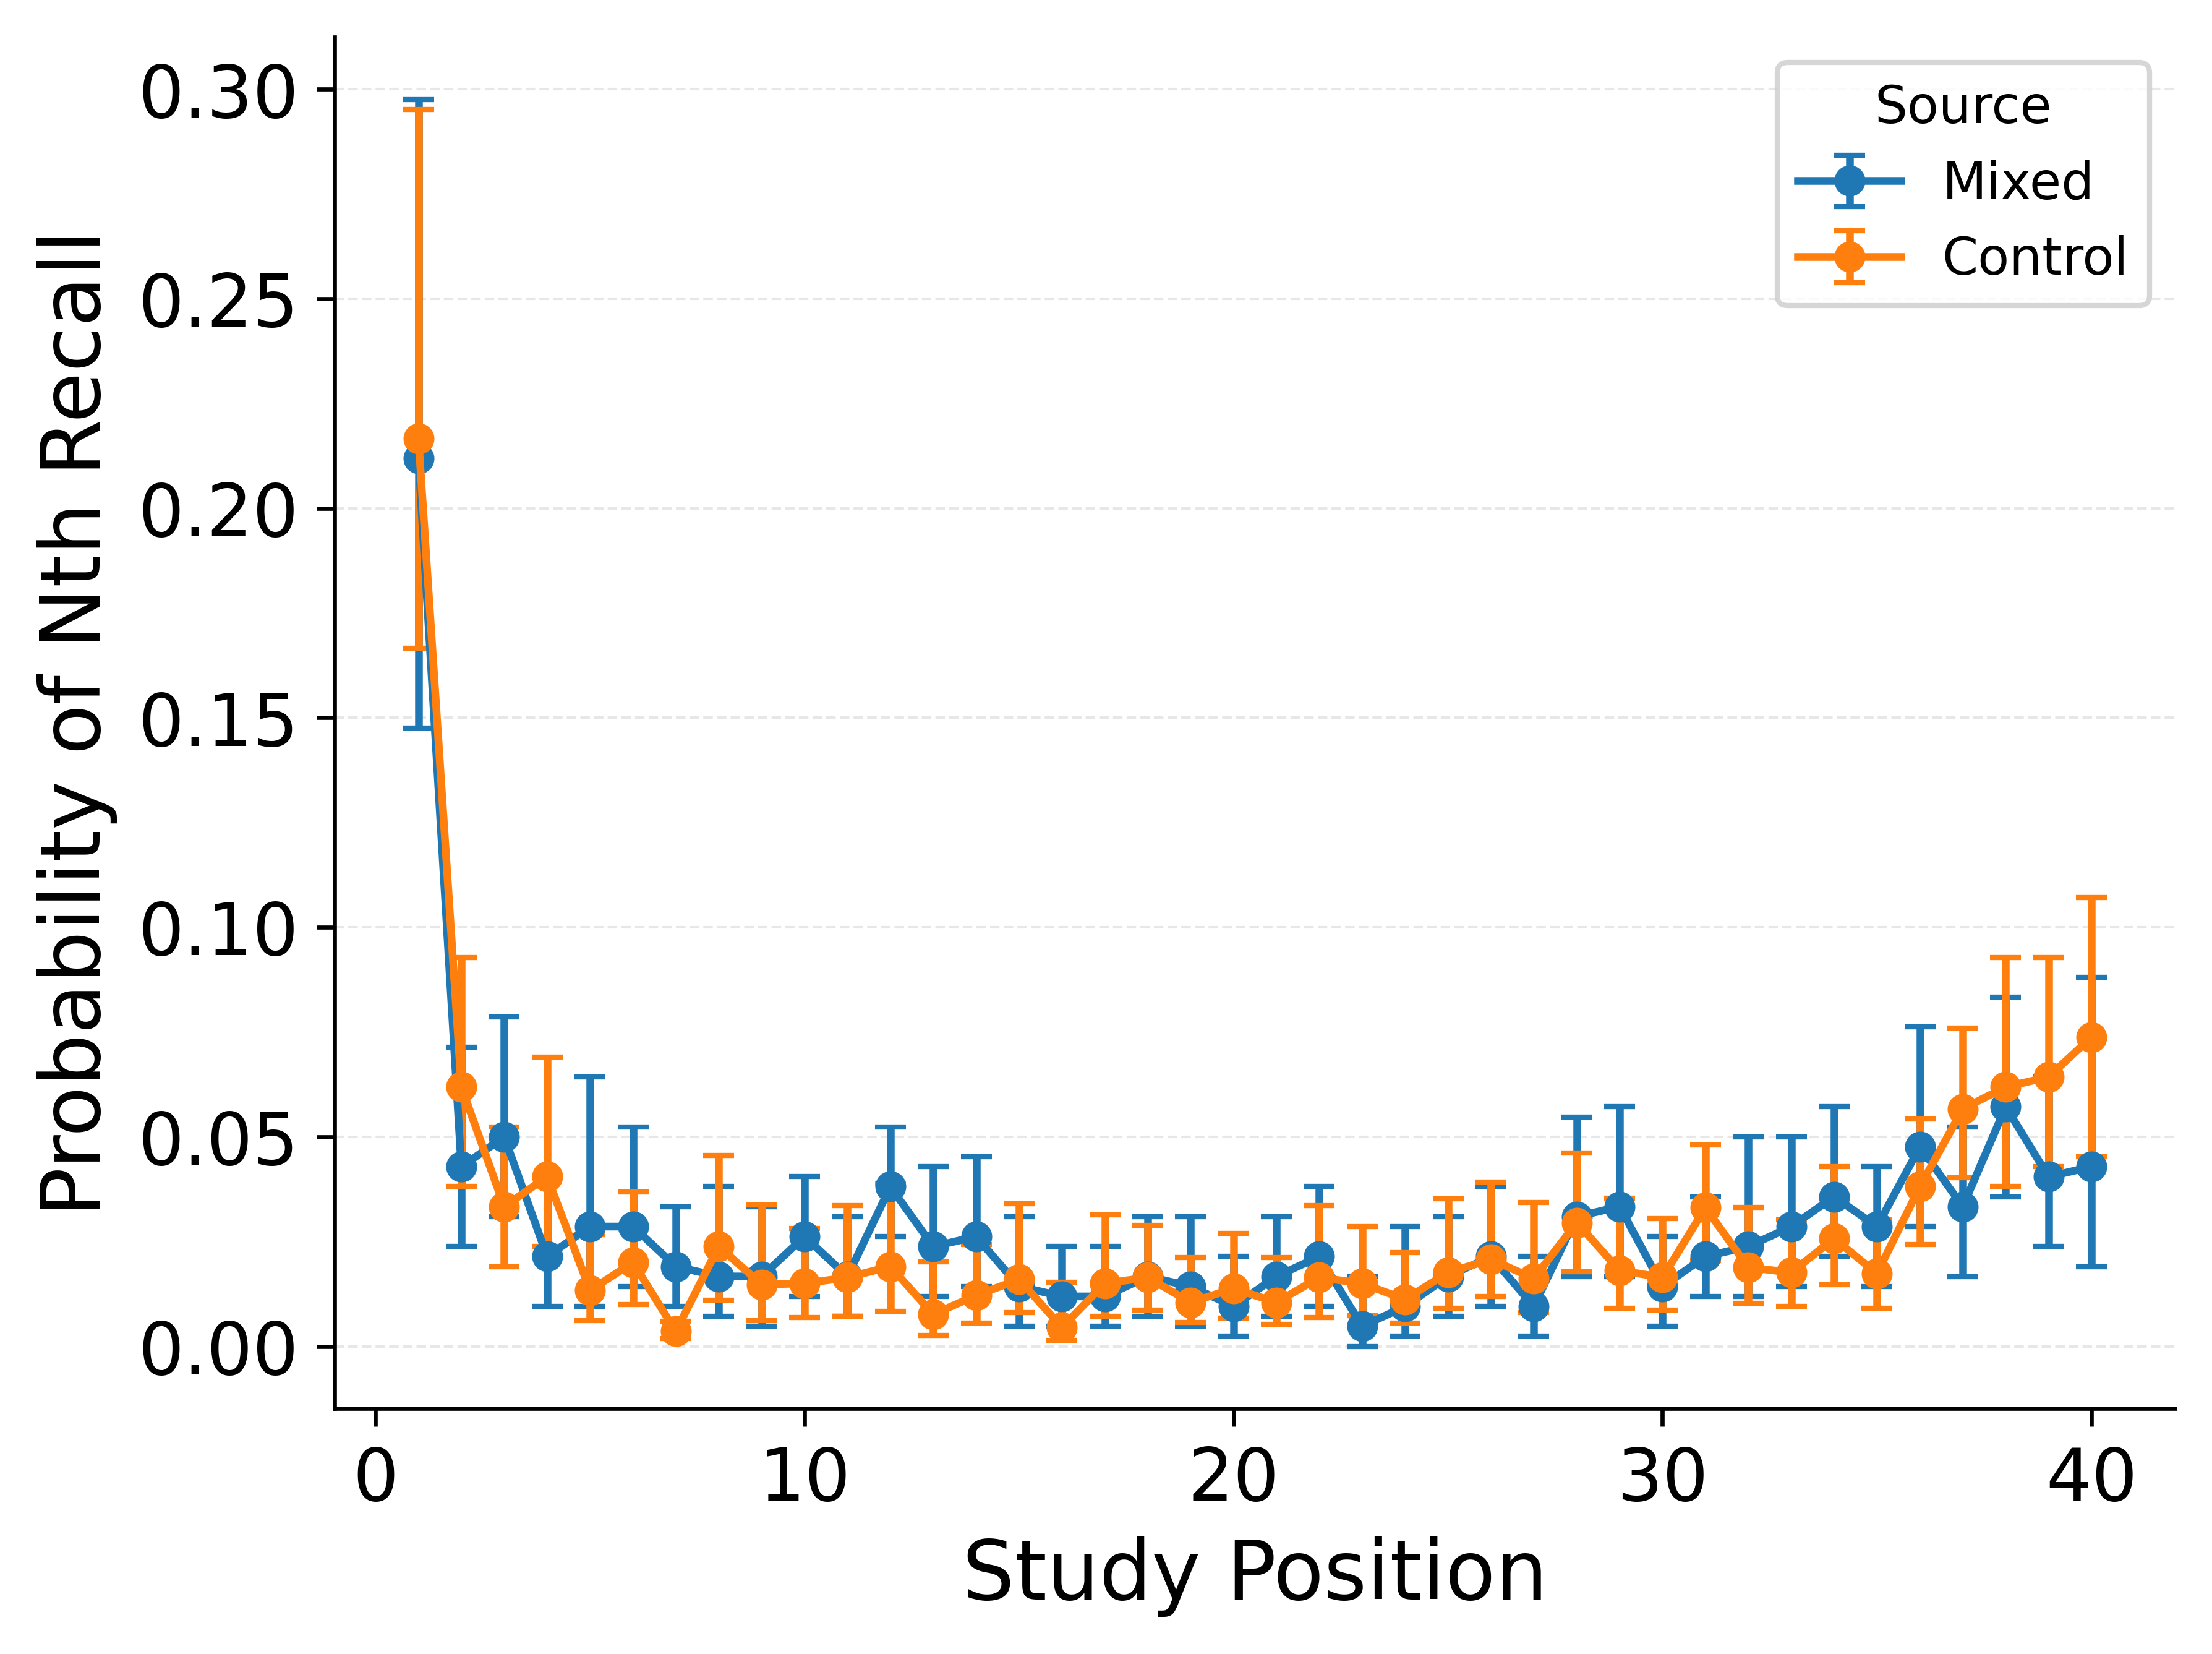
\includegraphics{../../work/thesis/figures/LohnasKahana2014_mixedvscontrolA_data_full_best_of_3_LT4_pnr.png}\end{minipage}%

\end{figure}%

\begin{figure}

\caption{\label{fig-cmr_benchmarks}Standard CMR predictions for mixed
and control list trials from trials from Lohnas and Kahana
(\citeproc{ref-lohnas2014retrieved}{2014}), with symmetric scoring over
matched serial positions of repeated items. Left: recall rate by serial
position (serial position curve, SPC). Middle: conditional response
probability (CRP) by lag. Right: probability of first recall by serial
position.}

\begin{minipage}{0.50\linewidth}
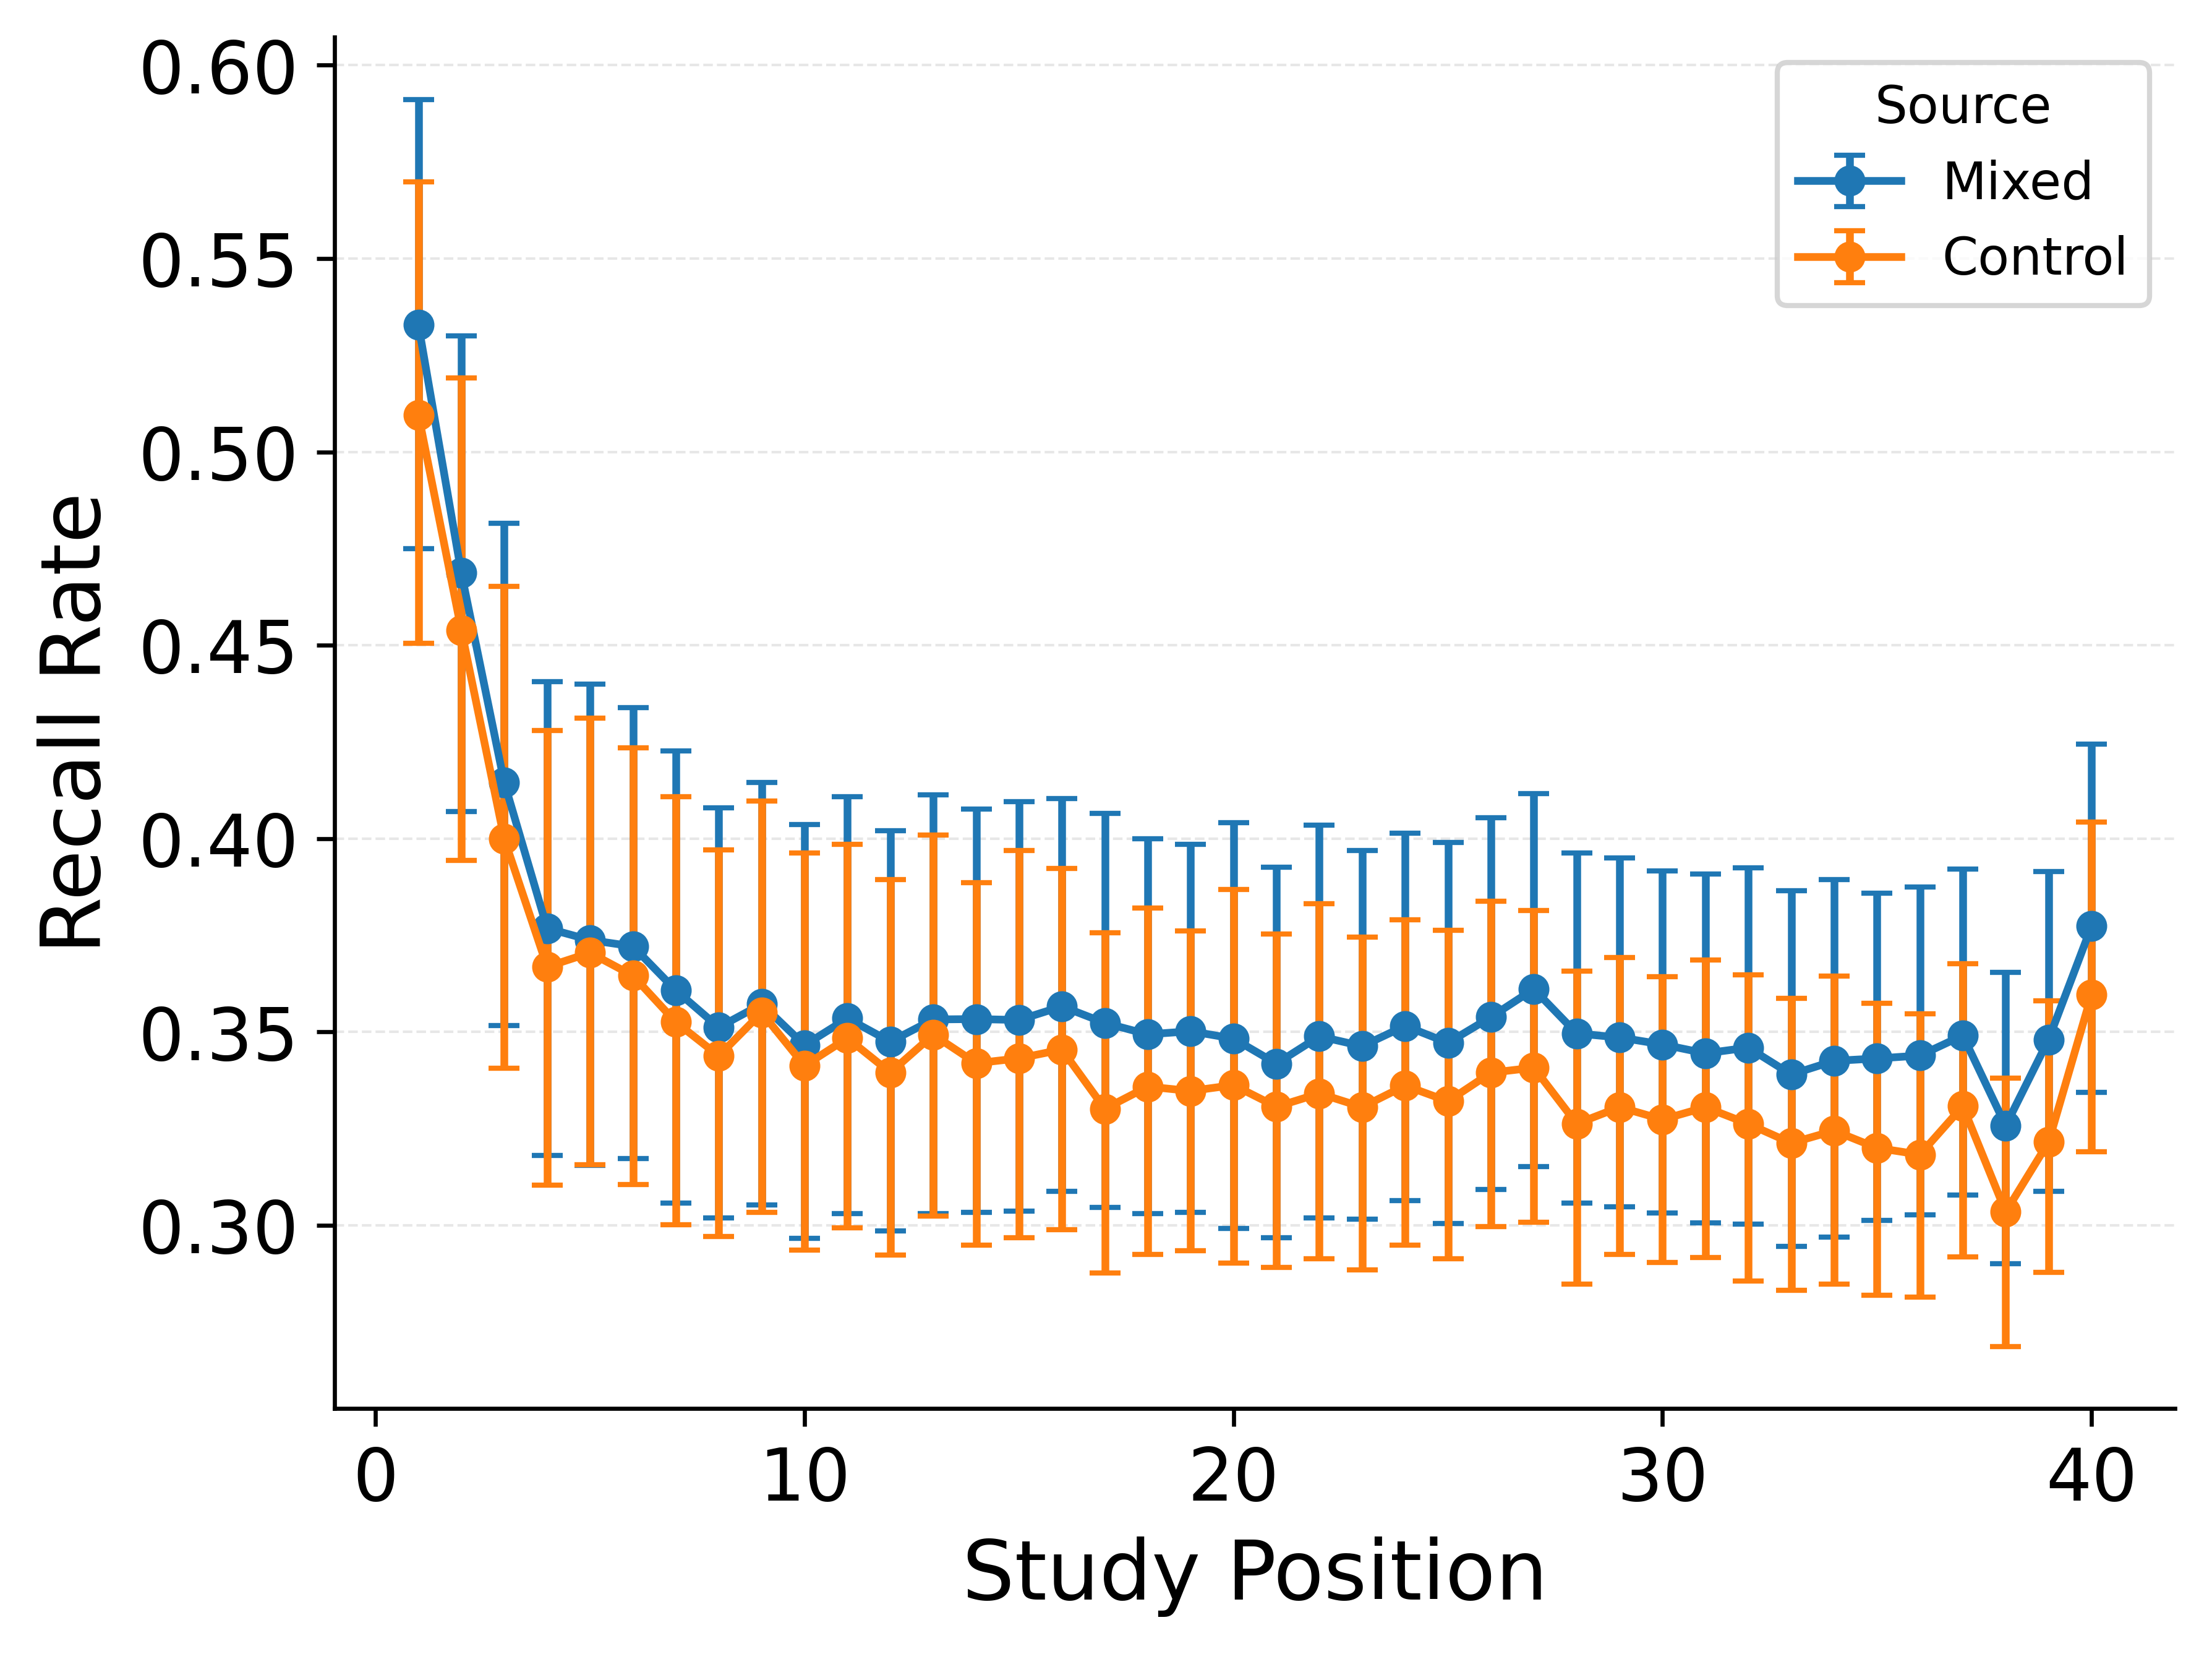
\includegraphics{../../work/thesis/figures/LohnasKahana2014_mixedvscontrolA_WeirdCMR_full_best_of_3_LT4_spc.png}\end{minipage}%
%
\begin{minipage}{0.50\linewidth}
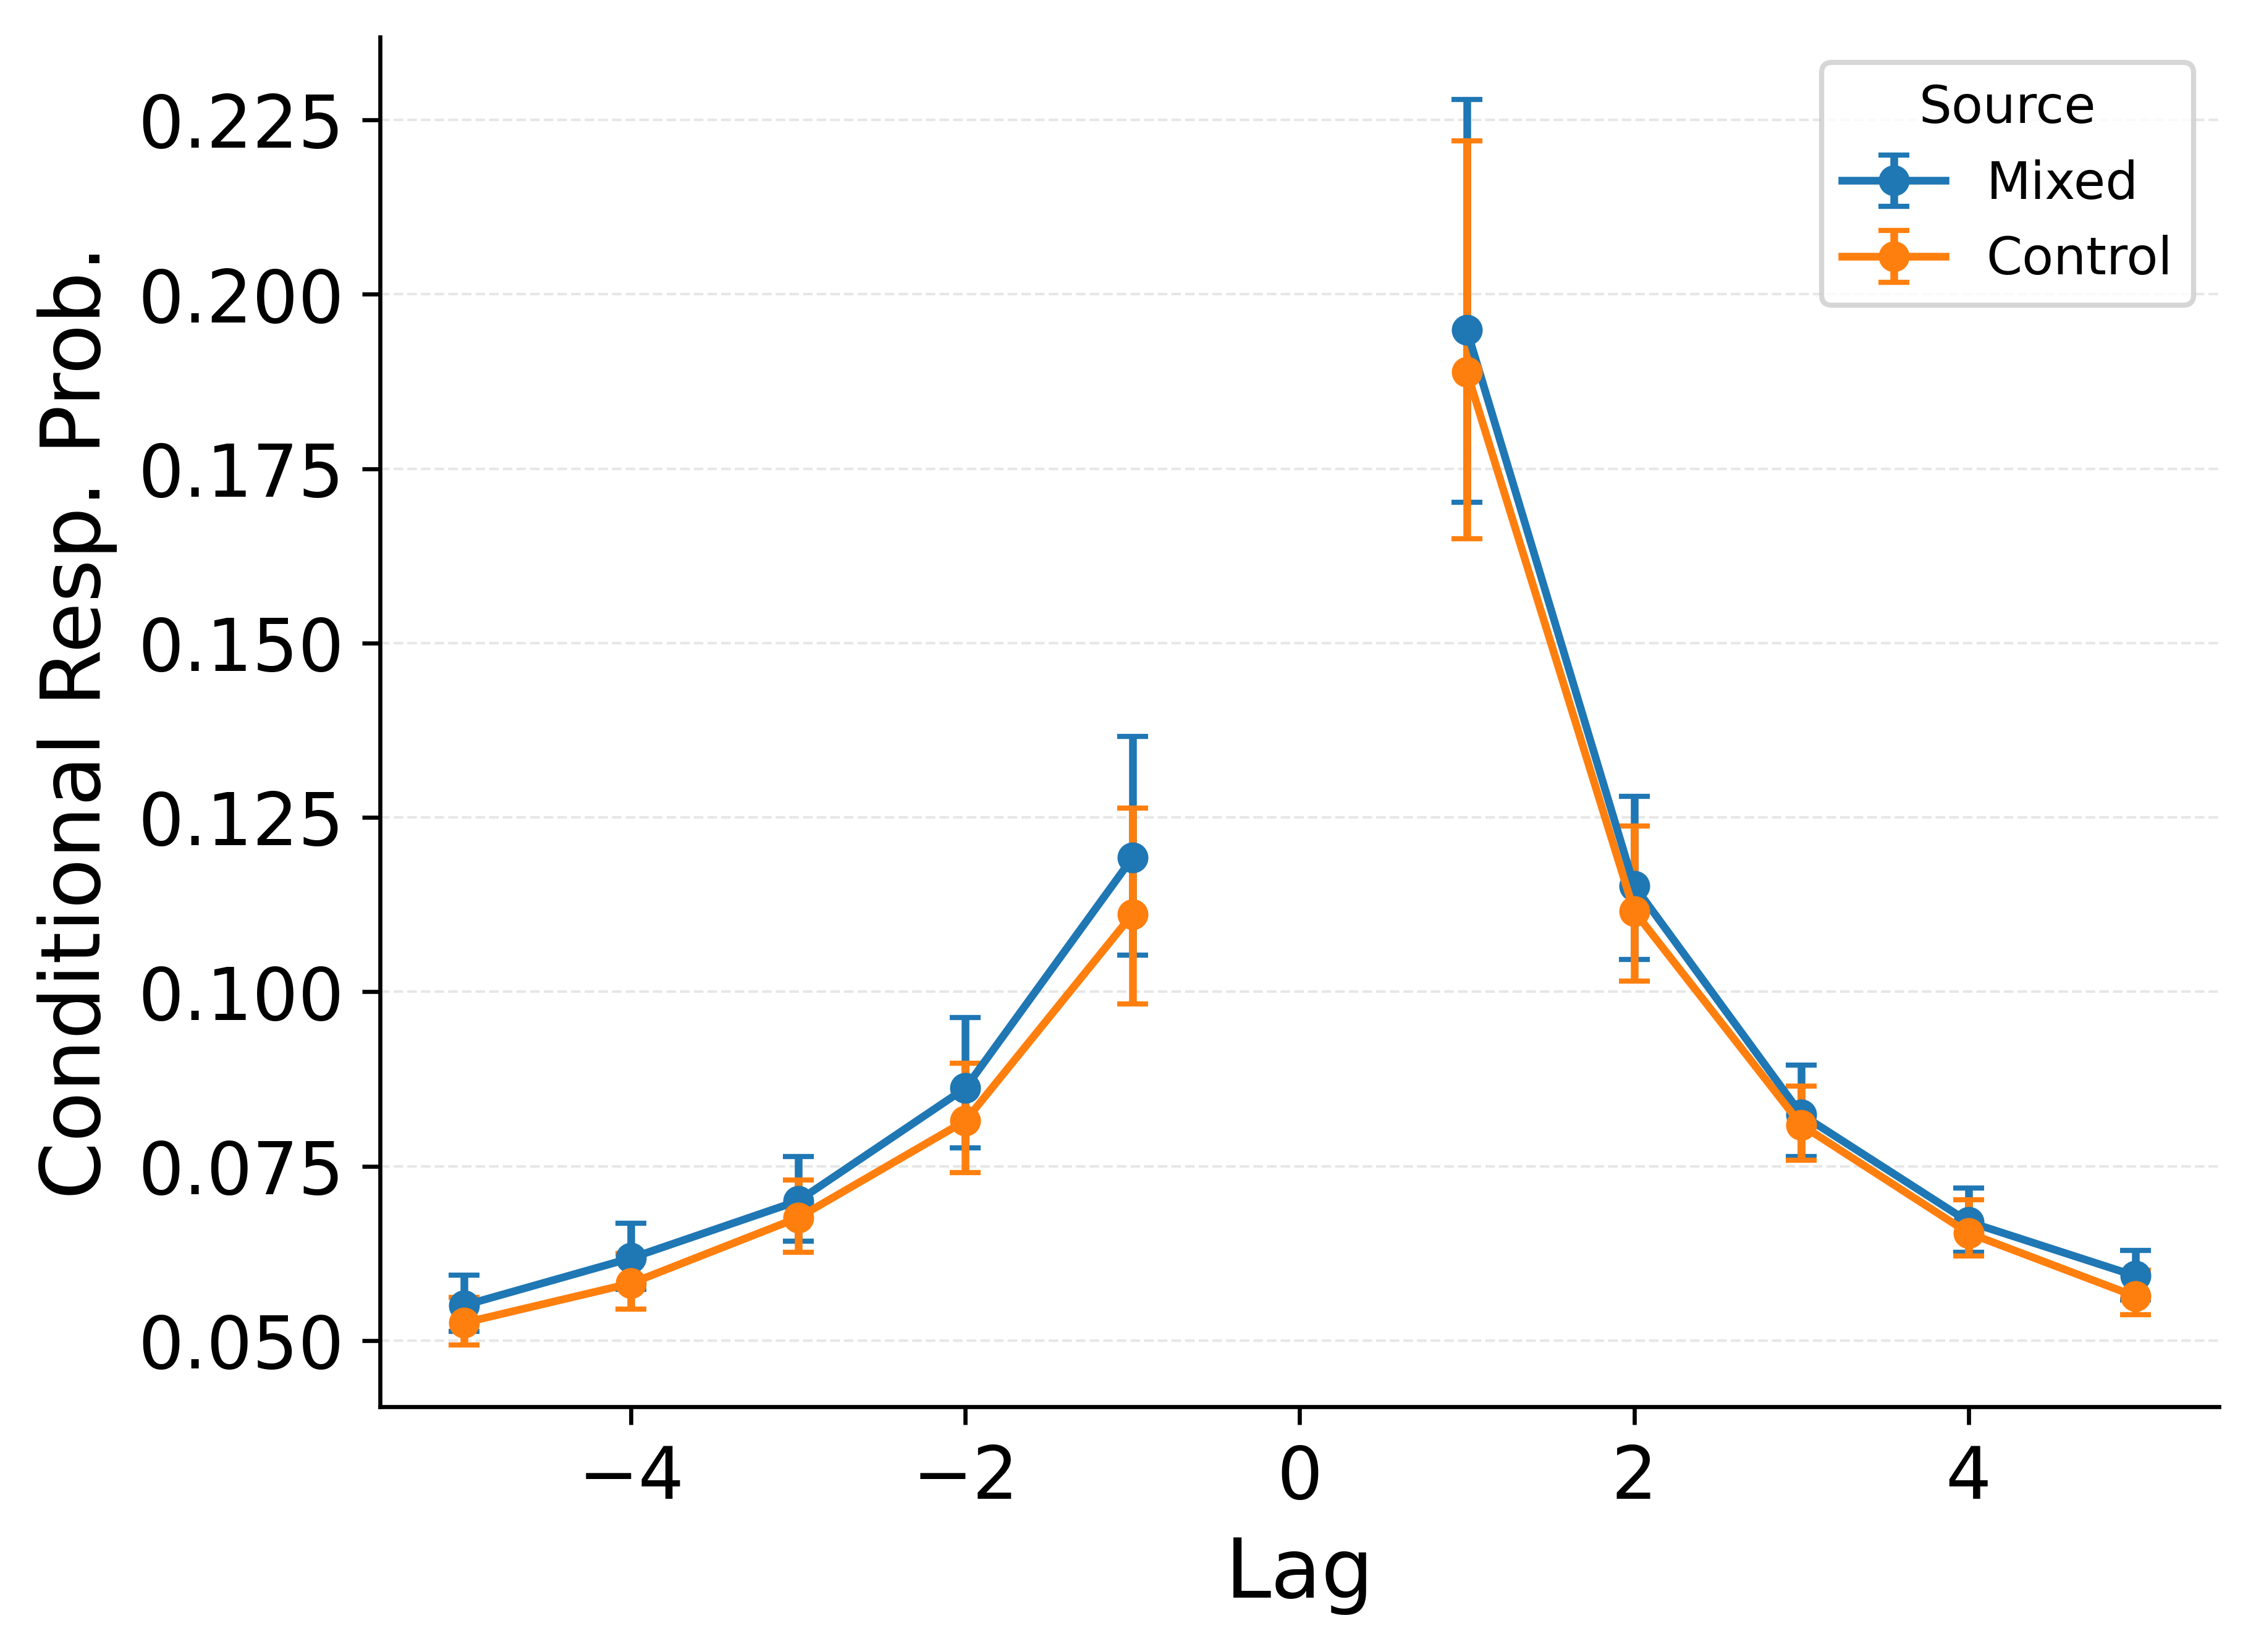
\includegraphics{../../work/thesis/figures/LohnasKahana2014_mixedvscontrolA_WeirdCMR_full_best_of_3_LT4_crp.png}\end{minipage}%
\newline
\begin{minipage}{\linewidth}
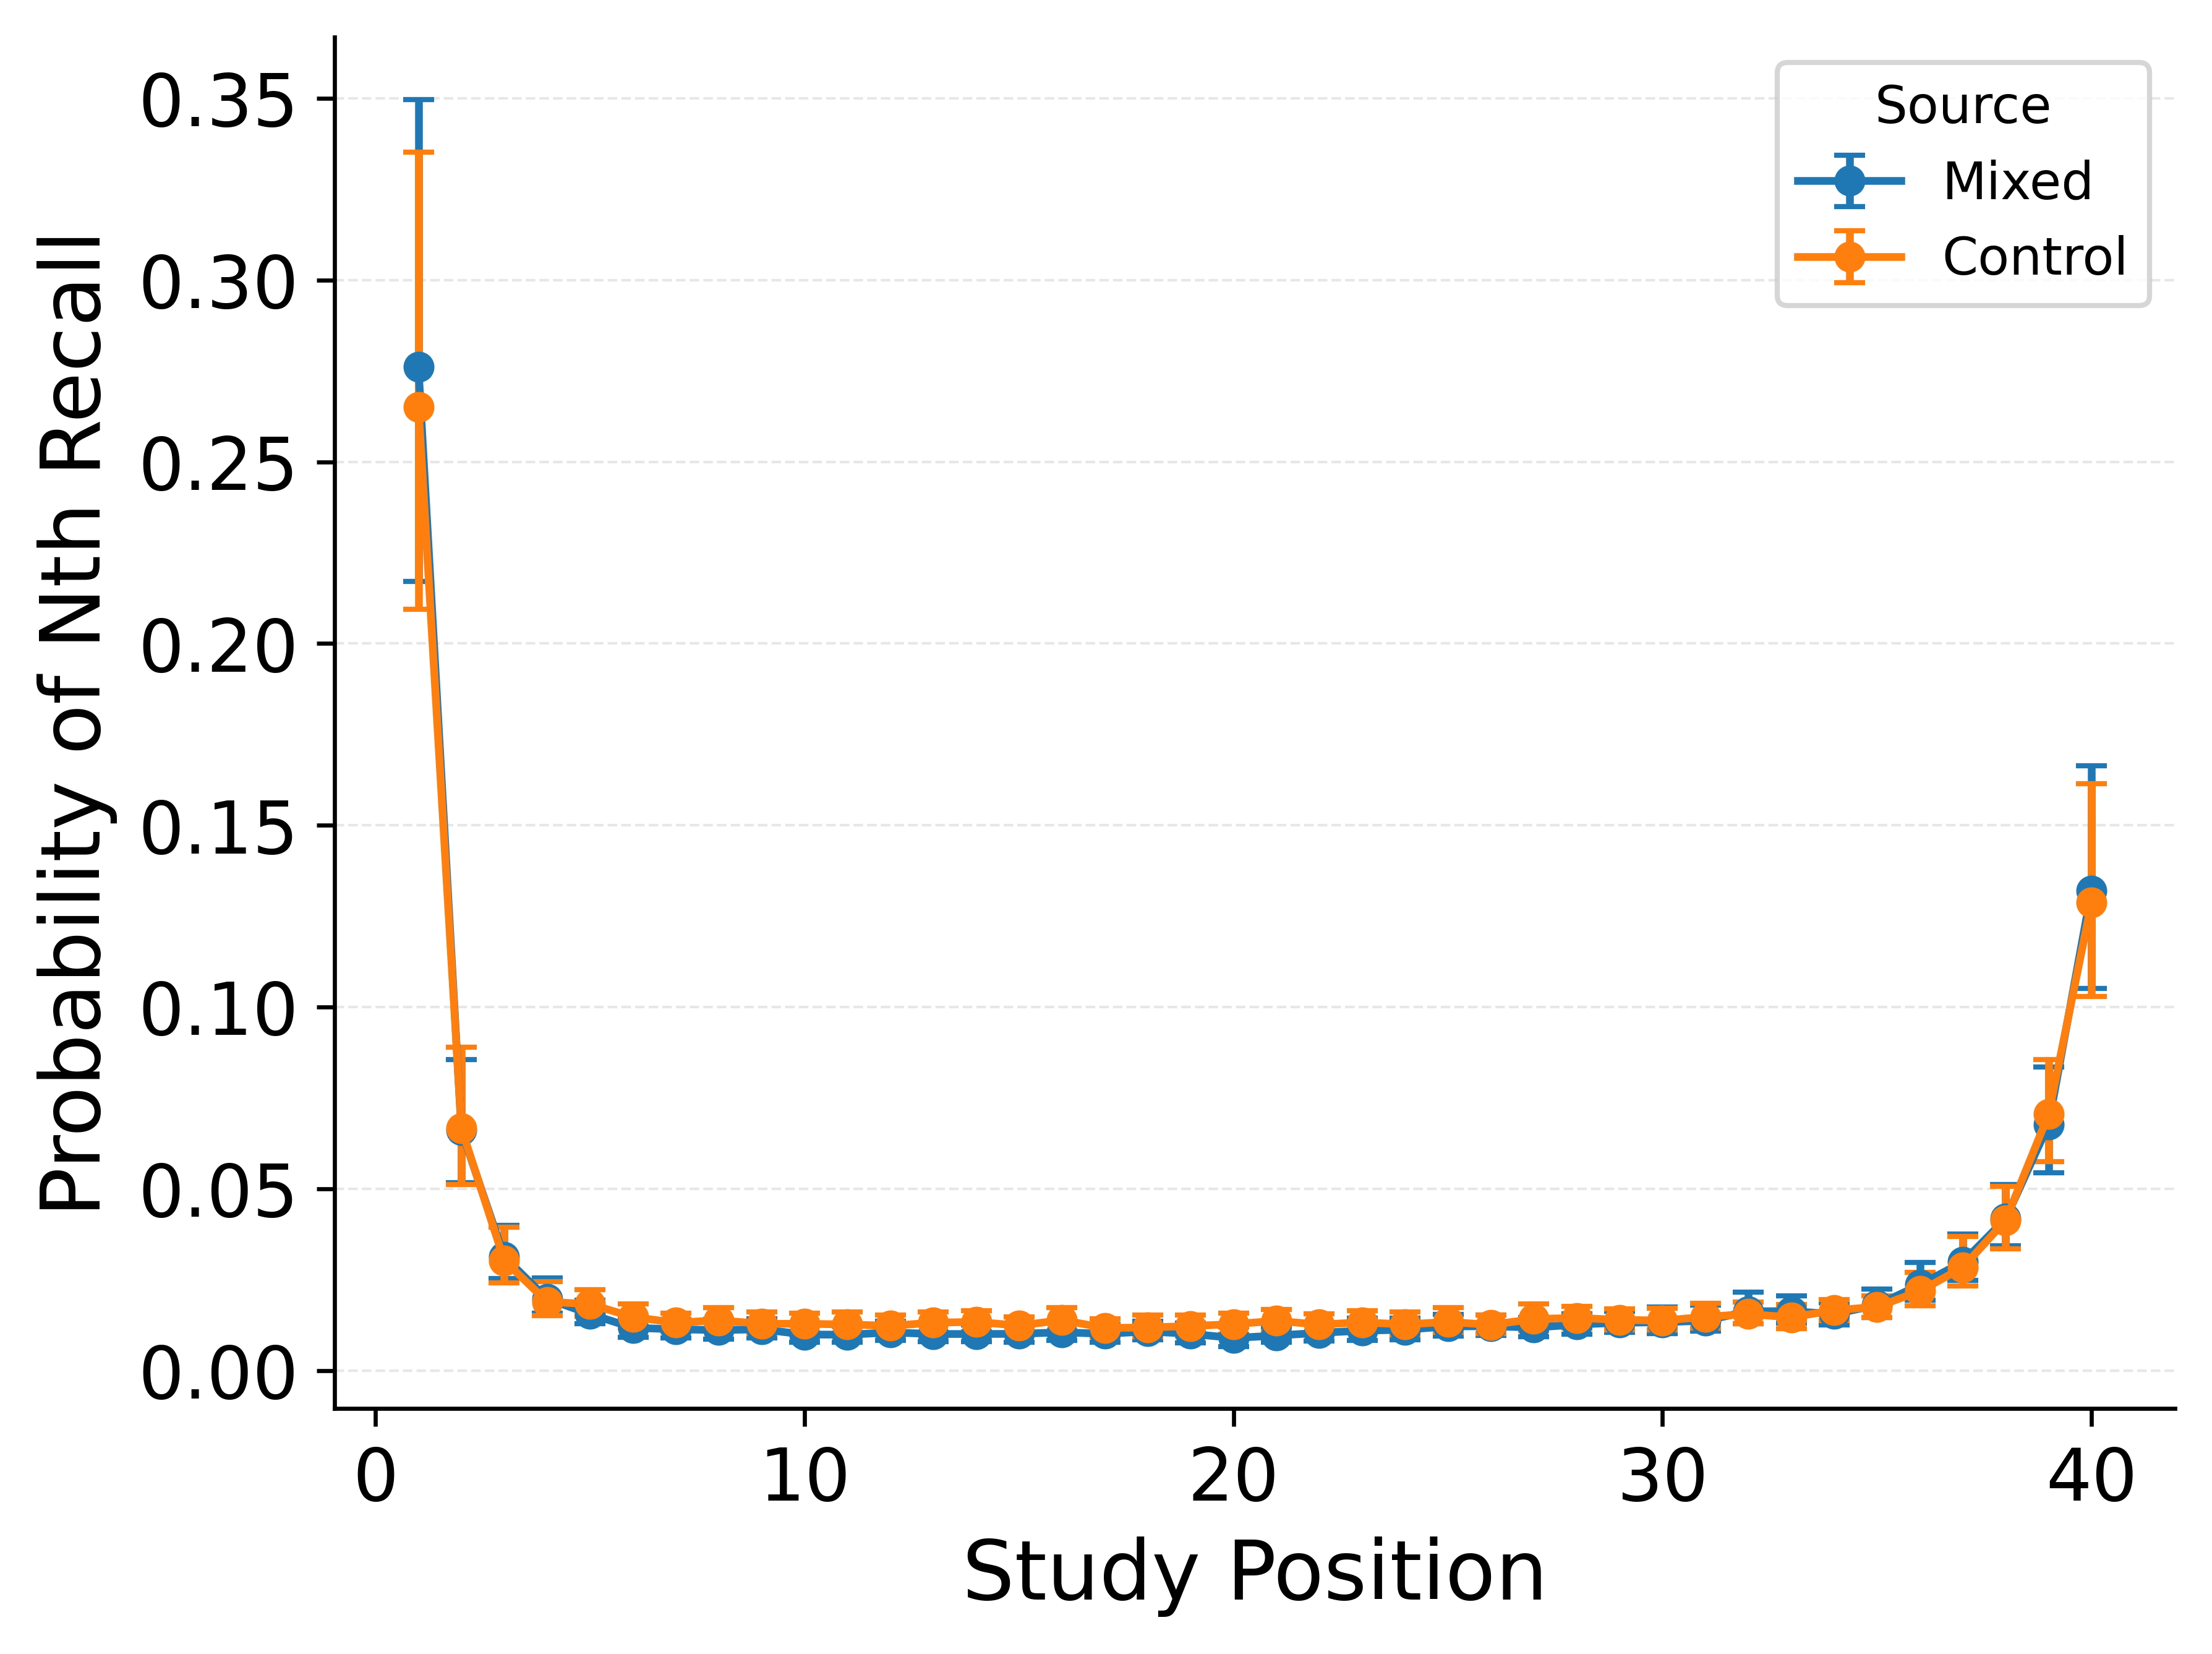
\includegraphics{../../work/thesis/figures/LohnasKahana2014_mixedvscontrolA_WeirdCMR_full_best_of_3_LT4_pnr.png}\end{minipage}%

\end{figure}%

\subsection{The Spacing Effect}\label{the-spacing-effect}

The spacing effect is classically understood as a repetition effect, and
has been a central focus of research on memory for repeated experience
(\citeproc{ref-cepeda2006distributed}{Cepeda et al., 2006}) However, it
applies even to pairs of distinct items, not just repeated items. By
measuring the probability of retrieving either of two study items during
a free recall trial -- an analysis termed the ``OR score'' -- research
often finds that pairs of spaced items were more likely to be recalled
than pairs of massed items (\citeproc{ref-lohnas2011contextual}{Lohnas
et al., 2011}). Notably, in a phenomenon called ``superadditivity'', the
mnemonic benefit of spacing is argued to be more pronounced for repeated
items than for distinct items. The probability of recalling an item
repeated in a spaced fashion may be higher than the probability of
recalling one of two distinct but similarly spaced items, violating
statistical independence
(\citeproc{ref-benjamin2010distributed}{Benjamin \& Tullis, 2010}).
Study-phase retrieval or other mechanisms specific to item repetitions
are thought to complement contextual variability mechanisms to produce
such superadditivity.

Figure~\ref{fig-spacing} displays the spacing function for mixed and
control lists in Lohnas and Kahana
(\citeproc{ref-lohnas2014retrieved}{2014}) alongside fitted CMR
simulations. In the data, the spacing function estimated from mixed
lists appears steeper than the function derived from our
position-matched, symmetric baseline (left panel of
Figure~\ref{fig-spacing}). Because the baseline equates list length,
presentation schedule, and scoring opportunity, the slope difference
cannot be attributed to serial-position or scoring artifacts; it
suggests a repetition-specific boost over and above the spacing effect
observed for equally spaced distinct items (i.e., a superadditive
component). Standard CMR, by contrast, reproduces the overall monotonic
spacing advantage but shows no apparent corresponding slope separation
between mixed and baseline conditions (right panel of
Figure~\ref{fig-spacing}). Thus, while CMR captures the basic
memorability gain with increasing lag, it does not express the
additional repetition-specific steepening present in the data.

\begin{figure}

\caption{\label{fig-spacing}The spacing effect for mixed vs control list
trials from Lohnas and Kahana
(\citeproc{ref-lohnas2014retrieved}{2014}). Left: data, right:
simulations of standard CMR fitted to the data.}

\begin{minipage}{0.50\linewidth}
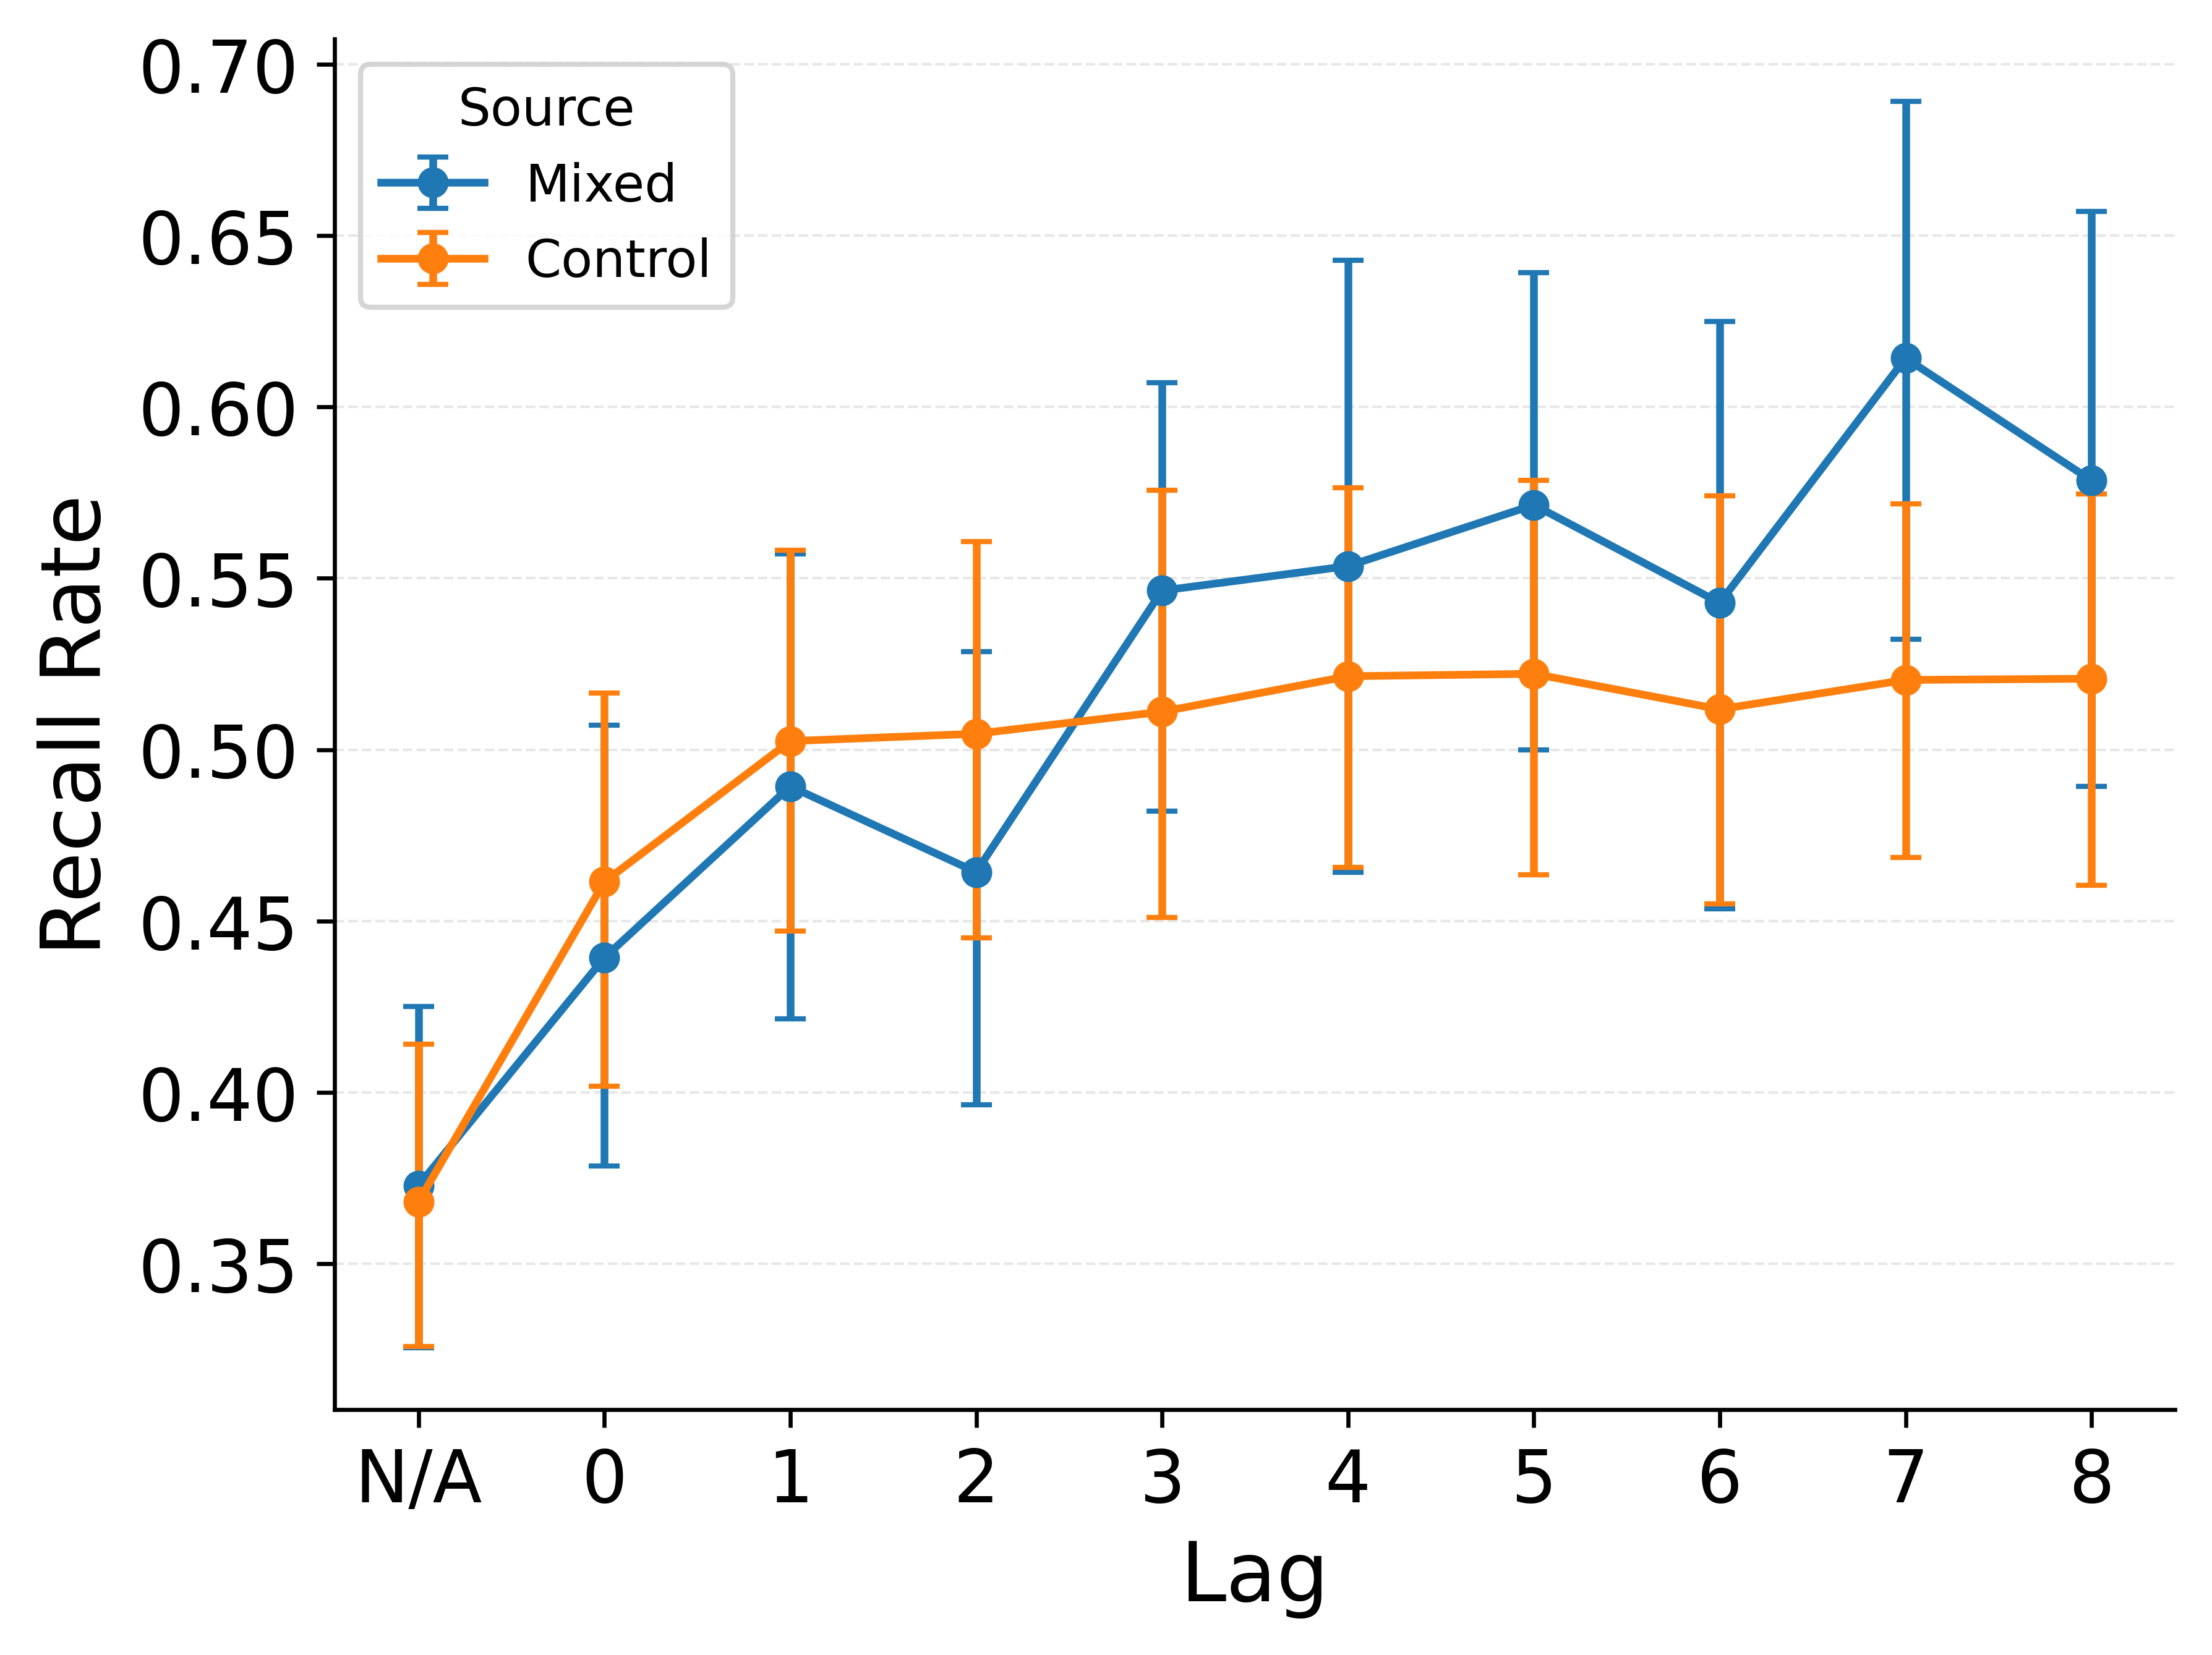
\includegraphics{../../work/thesis/figures/RepeatedRecallsLohnasKahana2014_mixedvscontrolA_data_full_best_of_3_LT4_full_rpl.png}\end{minipage}%
%
\begin{minipage}{0.50\linewidth}
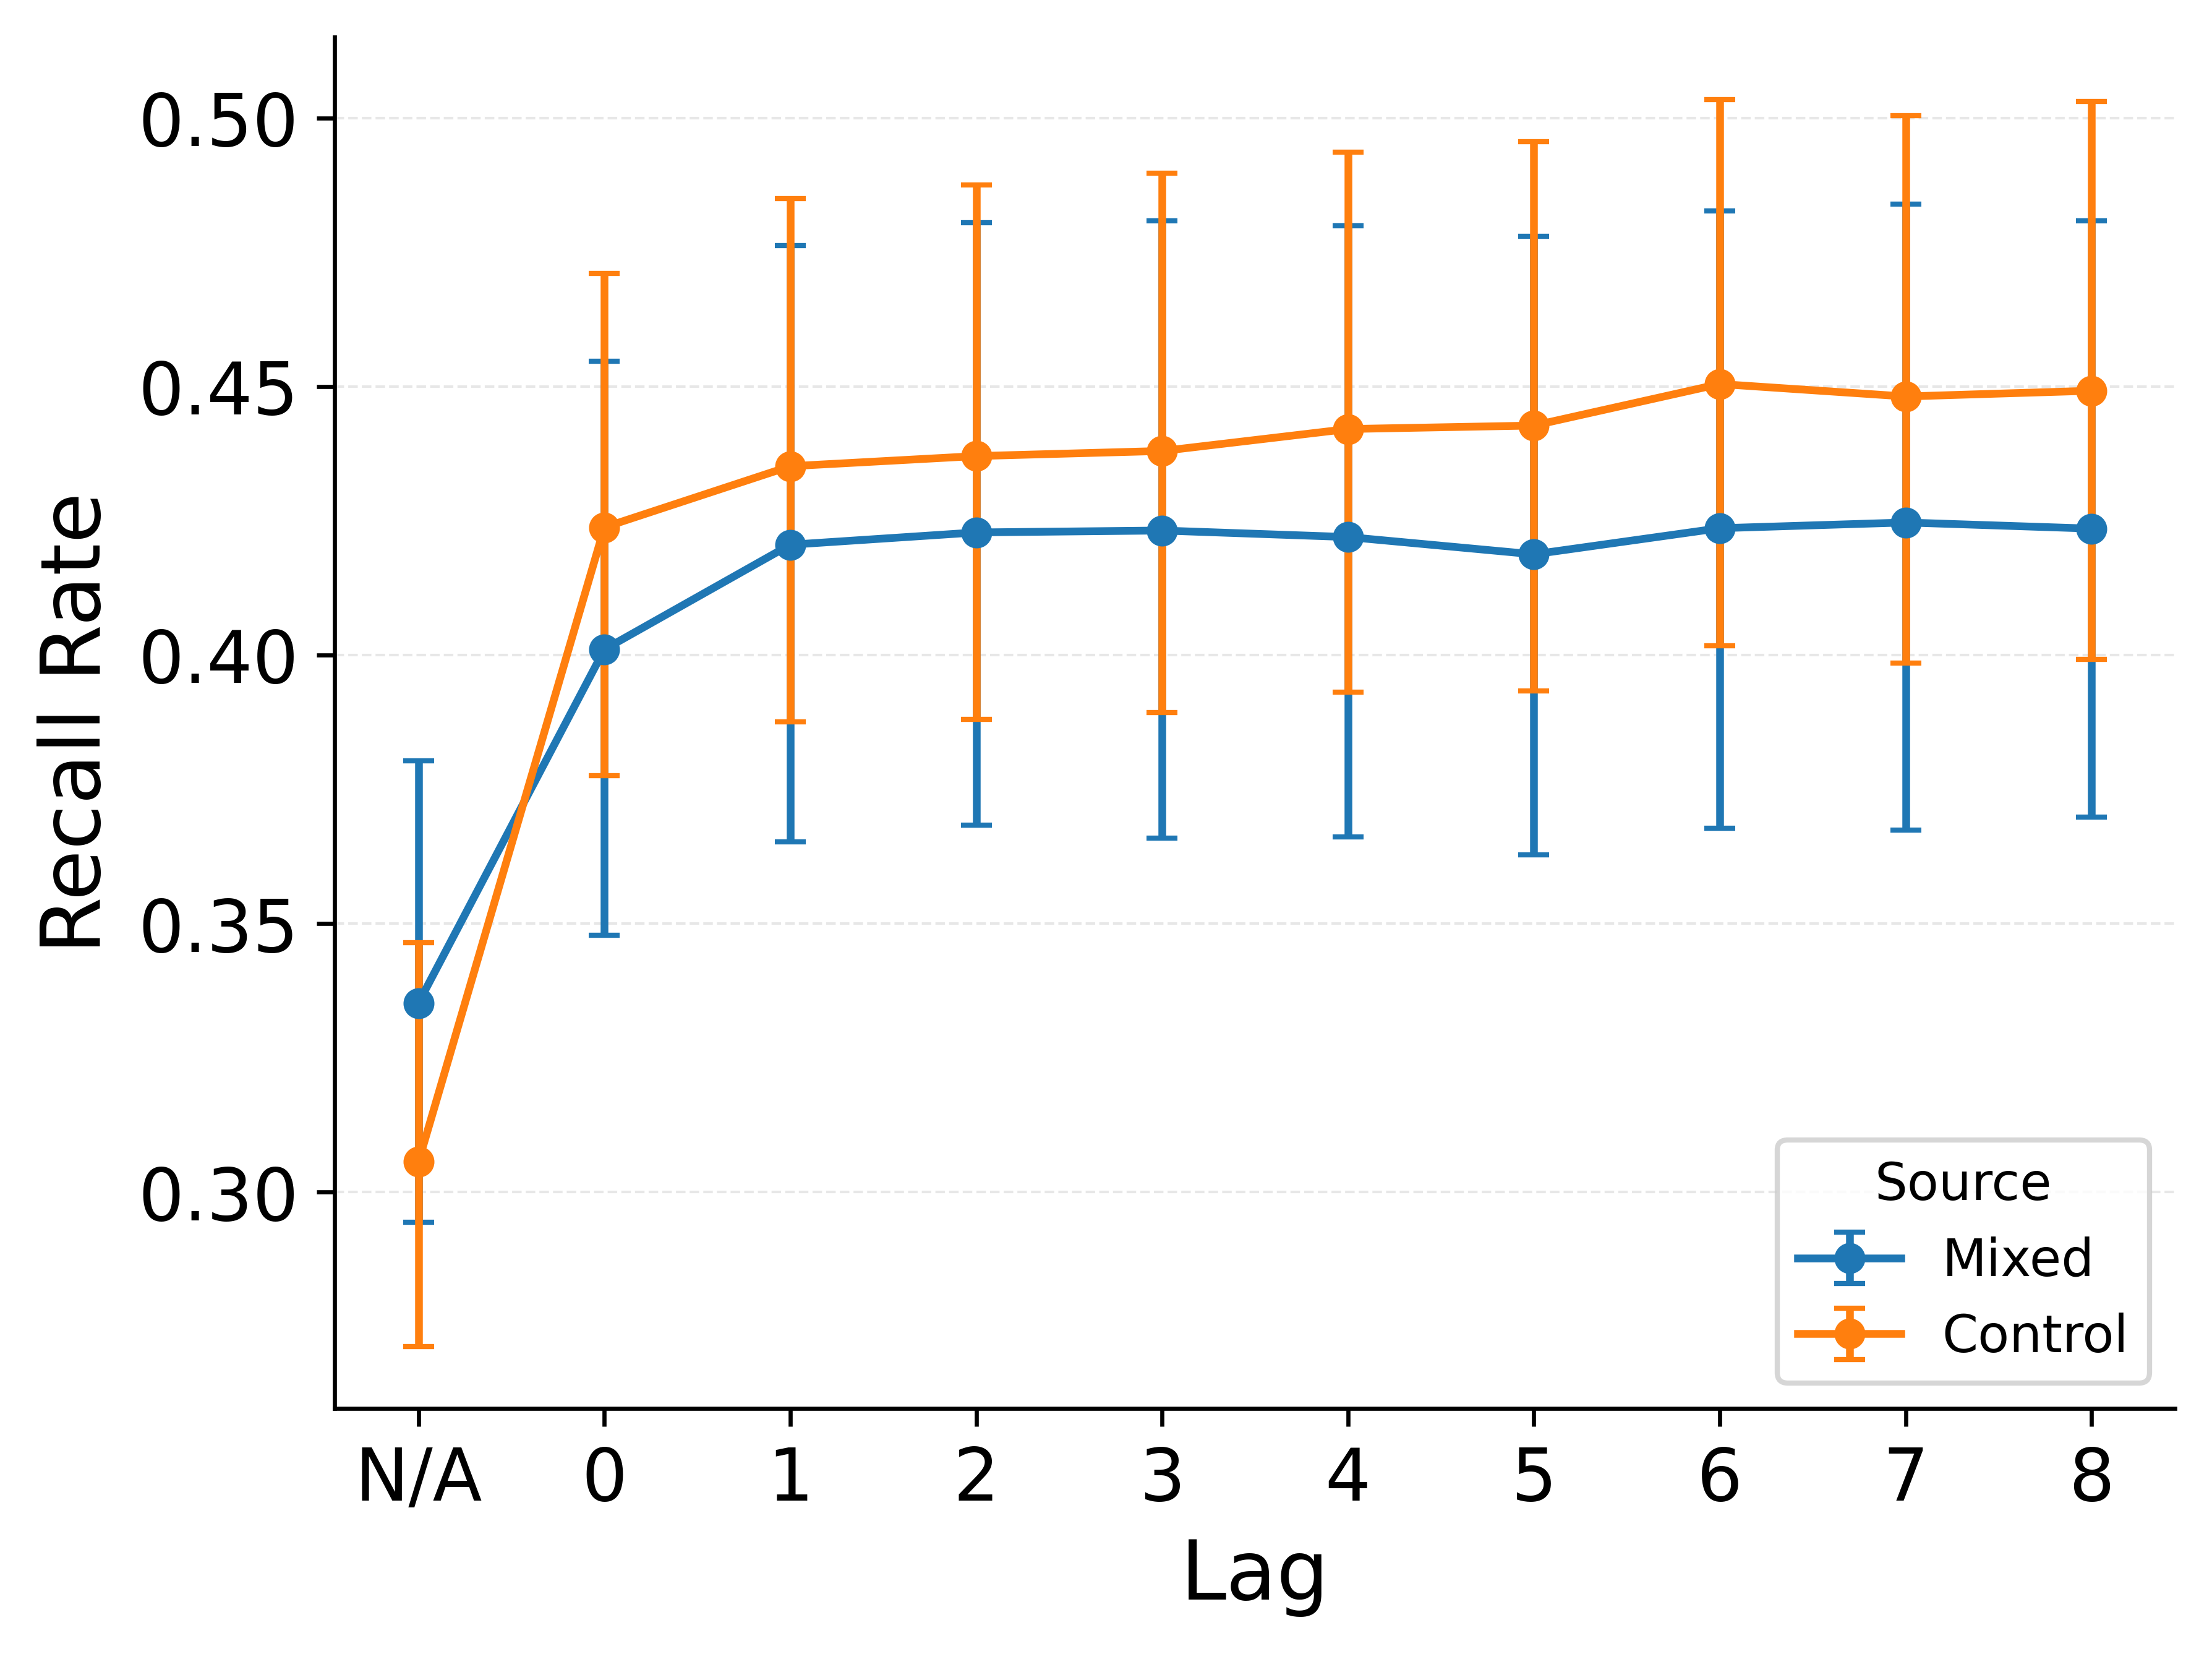
\includegraphics{../../work/thesis/figures/LohnasKahana2014_mixedvscontrolA_WeirdCMR_full_best_of_3_LT4_full_rpl.png}\end{minipage}%

\end{figure}%

\section{Diagnostic Tests of Cross-Occurrence Associative
Interference}\label{diagnostic-tests-of-cross-occurrence-associative-interference}

\subsection{Analytic definitions}\label{analytic-definitions}

All analyses use the matched, symmetric baseline defined above. For each
mixed-list trial with a repeater at positions \(i\) and \(j\), we pair
many control-list trials that match list length and presentation
schedule; in each control list we designate \(i\) and \(j\) as a single
pseudo-repeater and apply symmetric scoring. Unless noted, conditional
probabilities are computed over eligible transitions (targets exist and
have not yet been recalled), aggregated within participant, and then
averaged across participants. Mixed--minus--baseline contrasts isolate
the contribution of repetition structure.

\subsubsection{Repetition lag-CRP
(outgoing)}\label{repetition-lag-crp-outgoing}

\begin{figure}

\caption{\label{fig-rep-crp-base}\textbf{The repetition lag-CRP.}
\emph{A.} The lag-contiguity effect conceptualizes free-recall search as
movement along a mental timeline, but repeated items occupy two
positions on that timeline. \emph{B.} Extending the lag-CRP, we tabulate
transitions from a recalled repeater relative to both its study
positions. Illustration from mixed lists in Lohnas and Kahana
(\citeproc{ref-lohnas2014retrieved}{2014}).}

\begin{minipage}{0.50\linewidth}

\subcaption{\label{fig-rep-crp-schematic}}

\centering{

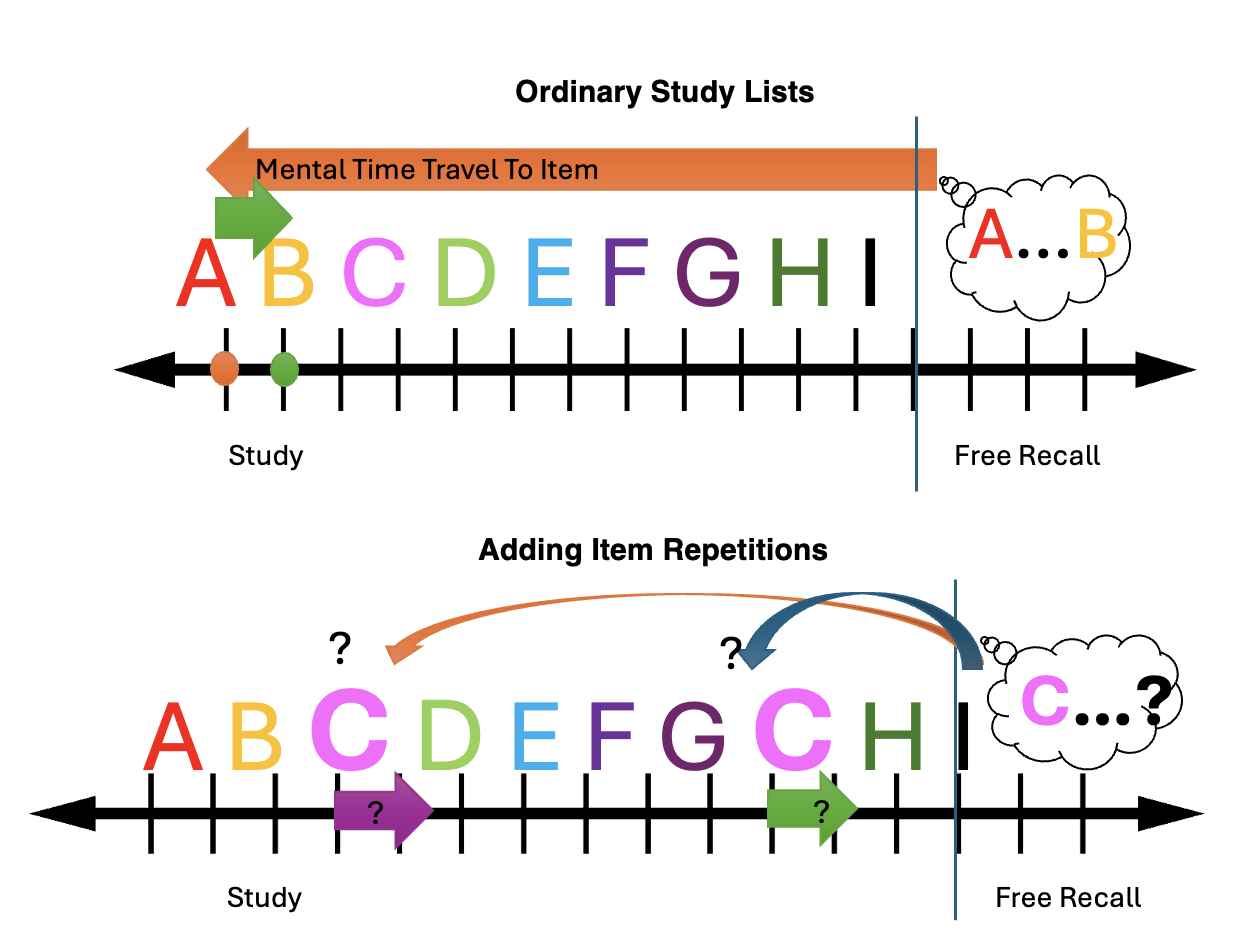
\includegraphics{../../work/thesis/repeat_cmr_figures/rep_lag_crp_schematic.png}

}

\end{minipage}%
%
\begin{minipage}{0.50\linewidth}

\subcaption{\label{fig-rep-crp-base}}

\centering{

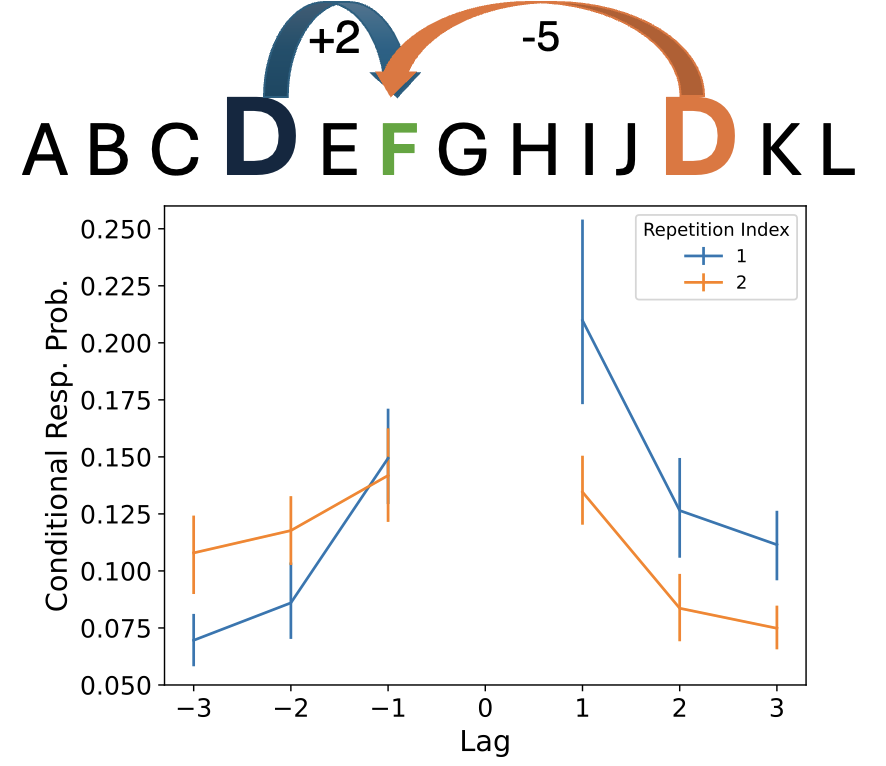
\includegraphics{../../work/thesis/repeat_cmr_figures/rep_crp_base.png}

}

\end{minipage}%

\end{figure}%

The goal is to test whether retrieving a repeater reinstates a composite
of its occurrence-specific contexts (blending) or selectively routes
through one occurrence (occurrence-specific access). For every recall of
a repeater with study positions \(i\) and \(j\) (\(i<j\)), we construct
two centered lag-CRPs: one treating \(i\) as the center and one treating
\(j\) as the center. From the first-centered cue, a \(+1\) transition is
to position \(i{+}1\); from the second-centered cue, a \(+1\) transition
is to position \(j{+}1\). Each centered curve gives the probability of
the very next recall at each available lag, conditional on eligibility.

Interpretation proceeds by comparing mixed lists to the position-matched
baseline. Blending predicts that, relative to baseline, outgoing
transitions will be \emph{more balanced} across the two centers (reduced
separation of first- vs second-centered curves) because both occurrence
contexts contribute to the cue. Occurrence-specific reinstatement
predicts a \emph{preserved or enlarged separation}, typically favoring
the first occurrence (e.g., higher \(+1\) from the first center than
from the second).

\subsubsection{Repetition lag-CRP (incoming; ``backward''
variant)}\label{repetition-lag-crp-incoming-backward-variant}

This variant helps explore the extent to which any asymmetry in the
outgoing analysis arises from how repeaters are cued versus how they cue
what follows. For every recall of a repeater, we look one step back to
the immediately preceding recall and compute lags centered on the
repeater's first and second study positions. If the asymmetry is already
present on incoming transitions, list context before the repeater tends
to match one occurrence's neighborhood more than the other (a cue-driven
effect). If incoming curves show little asymmetry but outgoing curves
do, the asymmetry is more likely due to how the repeater
\emph{reinstates} context.

Because this measure conditions on the event that a repeater is
recalled, it helps separate how the search state approached the repeater
from how the repeater redirects the next step.

\subsubsection{Cross-occurrence neighbor contiguity (free
recall)}\label{cross-occurrence-neighbor-contiguity-free-recall}

Lohnas and Kahana (\citeproc{ref-lohnas2014retrieved}{2014}) introduced
a neighbor-contiguity test for cross-occurrence blending: if the
first-presentation context is reinstated at the second, neighborhoods
around the two presentations become associatively linked. They measured
the probability of transitions from a \(+1\) or \(+2\) neighbor of one
presentation to a \(+1\) or \(+2\) neighbor of the other, comparing
mixed lists to position-matched controls.

We preserve that intuition but refine both baseline and readout. First,
the matched baseline uses symmetric scoring over the two matched
positions, preserving their identity relation and avoiding inflation
that arises when matched positions are tallied independently. Second, we
recast neighbor-contiguity as a \emph{centered lag-CRP} triggered by a
neighbor of one occurrence and centered on the other occurrence. This
reveals the full \emph{shape} of cross-occurrence support rather than
only neighbor-to-neighbor bins.

Let a repeater appear at \(i\) and \(j\) with \(i<j\). In the
first-centered variant, triggers are recalls of \(j{+}1\) or \(j{+}2\);
for each trigger we record the next recall and compute its lag relative
to \(i\), tabulating a lag-CRP centered on \(i\) under the usual
eligibility constraints. The second-centered variant swaps roles, using
\(i{+}1\) or \(i{+}2\) as triggers and centering lags on \(j\). For each
variant we subtract the matched, symmetric baseline to obtain a
mixed--minus--baseline curve.

Blending predicts above-baseline mass near the alternative occurrence's
neighbors (e.g., elevated probability around \(\ell=\pm1,\pm2\) with the
typical forward skew), because the trigger in one neighborhood partially
reinstates the other neighborhood's context. Occurrence-specific access
predicts that the centered curves in mixed lists overlay their
baselines, indicating no selective elevation of cross-occurrence
neighbors.

Re-expressing neighbor-contiguity this way provides a
position-controlled contrast (via symmetric scoring) and a richer
diagnostic: the magnitude and spread of the centered curve show whether
cross-occurrence support is diffuse, localized, or absent. Because the
triggers are neighbors rather than the repeater itself, the analysis
remains sensitive to blending that operates without requiring the
repeated item to be recalled.

\subsubsection{Serial forward-chaining test (serial
recall)}\label{serial-forward-chaining-test-serial-recall}

This test asks whether blended support at retrieval increases
competition between continuations from the first versus second
occurrence in serial report. For repeated lists we focus on trials where
participants have reported the list correctly through position \(i\)
(the first occurrence). The correct continuation is the transition
\(i\rightarrow i{+}1\); the cross-occurrence competitor is
\(i\rightarrow j{+}1\). We compute the probabilities of the correct
chain and the cross-occurrence error, conditional on eligibility, and
compare to matched pseudo-repeater positions in controls. Blending
predicts an elevated error rate to \(j{+}1\) relative to baseline with a
corresponding reduction in correct forward chaining. Occurrence-specific
reinstatement predicts no elevation of \(i\rightarrow j{+}1\) errors
relative to baseline and intact chaining through \(i{+}1\).

We treat the matched control lists as the baseline for the error rate so
that any elevation reflects cross-occurrence competition rather than
serial-position structure.

\subsection{Cross-Occurrence Neighbor
Transitions}\label{cross-occurrence-neighbor-transitions}

This analysis tests whether repetition links the neighborhoods
surrounding the two study positions of a repeated item. We use the
centered lag-CRP recast described above, with triggers confined to
forward neighbors (+1 or +2) of one occurrence and lags centered on the
other occurrence, and we compare mixed lists to the matched, symmetric
baseline.

We examine two symmetric variants, shown in the top row of
Figure~\ref{fig-neighbor_contiguity}. In the \textbf{first→second}
variant (left column), transitions are triggered by recalls of the
forward neighbors of the first presentation (positions \(i{+}1\) or
\(i{+}2\)), and the lag-CRP is centered on the second presentation at
\(j\) (so \(\ell=\text{next}-j\)). In the \textbf{second→first} variant
(right column), triggers are the forward neighbors of the second
presentation (\(j{+}1\) or \(j{+}2\)), and the lag-CRP is centered on
the first presentation at \(i\) (so \(\ell=\text{next}-i\)). As before,
all probabilities condition on eligibility and the baseline uses
position-matched control lists with symmetric scoring.

Because study-phase reinstatement pulls the two occurrence contexts
together and retrieval reinstates a composite tied to the repeated item,
CMR predicts elevated cross-occurrence neighbor transitions in
\emph{both} directions: after a trigger in one neighborhood, the next
recall should be above baseline at the other neighborhood's immediate
lags (typically with the usual forward skew). These predictions are
confirmed in the simulations (bottom row of
Figure~\ref{fig-neighbor_contiguity}), which show clear above-baseline
mass near \(\ell=\pm1,\pm2\) in both variants.

The data tell a different story. In both variants,
mixed--minus--baseline curves show little to no elevation at the other
occurrence's neighbors (top row of
Figure~\ref{fig-neighbor_contiguity}). Thus, we do not see the predicted
knitting of the two neighborhoods. However, there is a selective effect
not anticipated by CMR: in the \textbf{first→second} variant (left),
transitions to the \emph{repeated item itself} (lag \(=0\), conditional
on availability) are elevated relative to baseline. This lag-0 bump does
not appear in the \textbf{second→first} variant (right), nor do we
observe the robust cross-neighbor boosts that CMR predicts in either
direction.

The absence of above-baseline neighbor-to-neighbor transitions argues
against a blended neighborhood linkage as the dominant consequence of
repetition. The asymmetric lag-0 elevation---visible only when moving
from the first occurrence's neighborhood toward the second---suggests
that repetition can heighten access to the repeated item without
knitting the two neighborhoods together. We return to this selective
lag-0 effect when introducing the ICMR-Reinf variant, which replaces
associative blending at study with reinforcement of the first-occurrence
trace and better accommodates this pattern.

\begin{figure}

\caption{\label{fig-neighbor_contiguity}Cross-occurrence neighbor
transitions as centered lag-CRPs (free recall). Top row (data), bottom
row (CMR simulations). \textbf{Left column (first→second):} triggers are
forward neighbors of the \emph{first} presentation (\(i{+}1,i{+}2\));
lags are centered on the \emph{second} presentation at \(j\) (so
\(\ell=\text{next}-j\)). \textbf{Right column (second→first):} triggers
are forward neighbors of the \emph{second} presentation
(\(j{+}1,j{+}2\)); lags are centered on the \emph{first} presentation at
\(i\) (so \(\ell=\text{next}-i\)). All curves plot
mixed--minus--matched-control probabilities using the symmetric
baseline. In the data, cross-occurrence neighbor bins (e.g.,
\(\ell=\pm1,\pm2\)) sit near baseline in both directions, with a
selective elevation at \(\ell=0\) (the repeater itself) only in the
first→second case. Standard CMR predicts pronounced above-baseline peaks
at the other occurrence's neighbors in both directions, consistent with
associative blending.}

\begin{minipage}{0.50\linewidth}
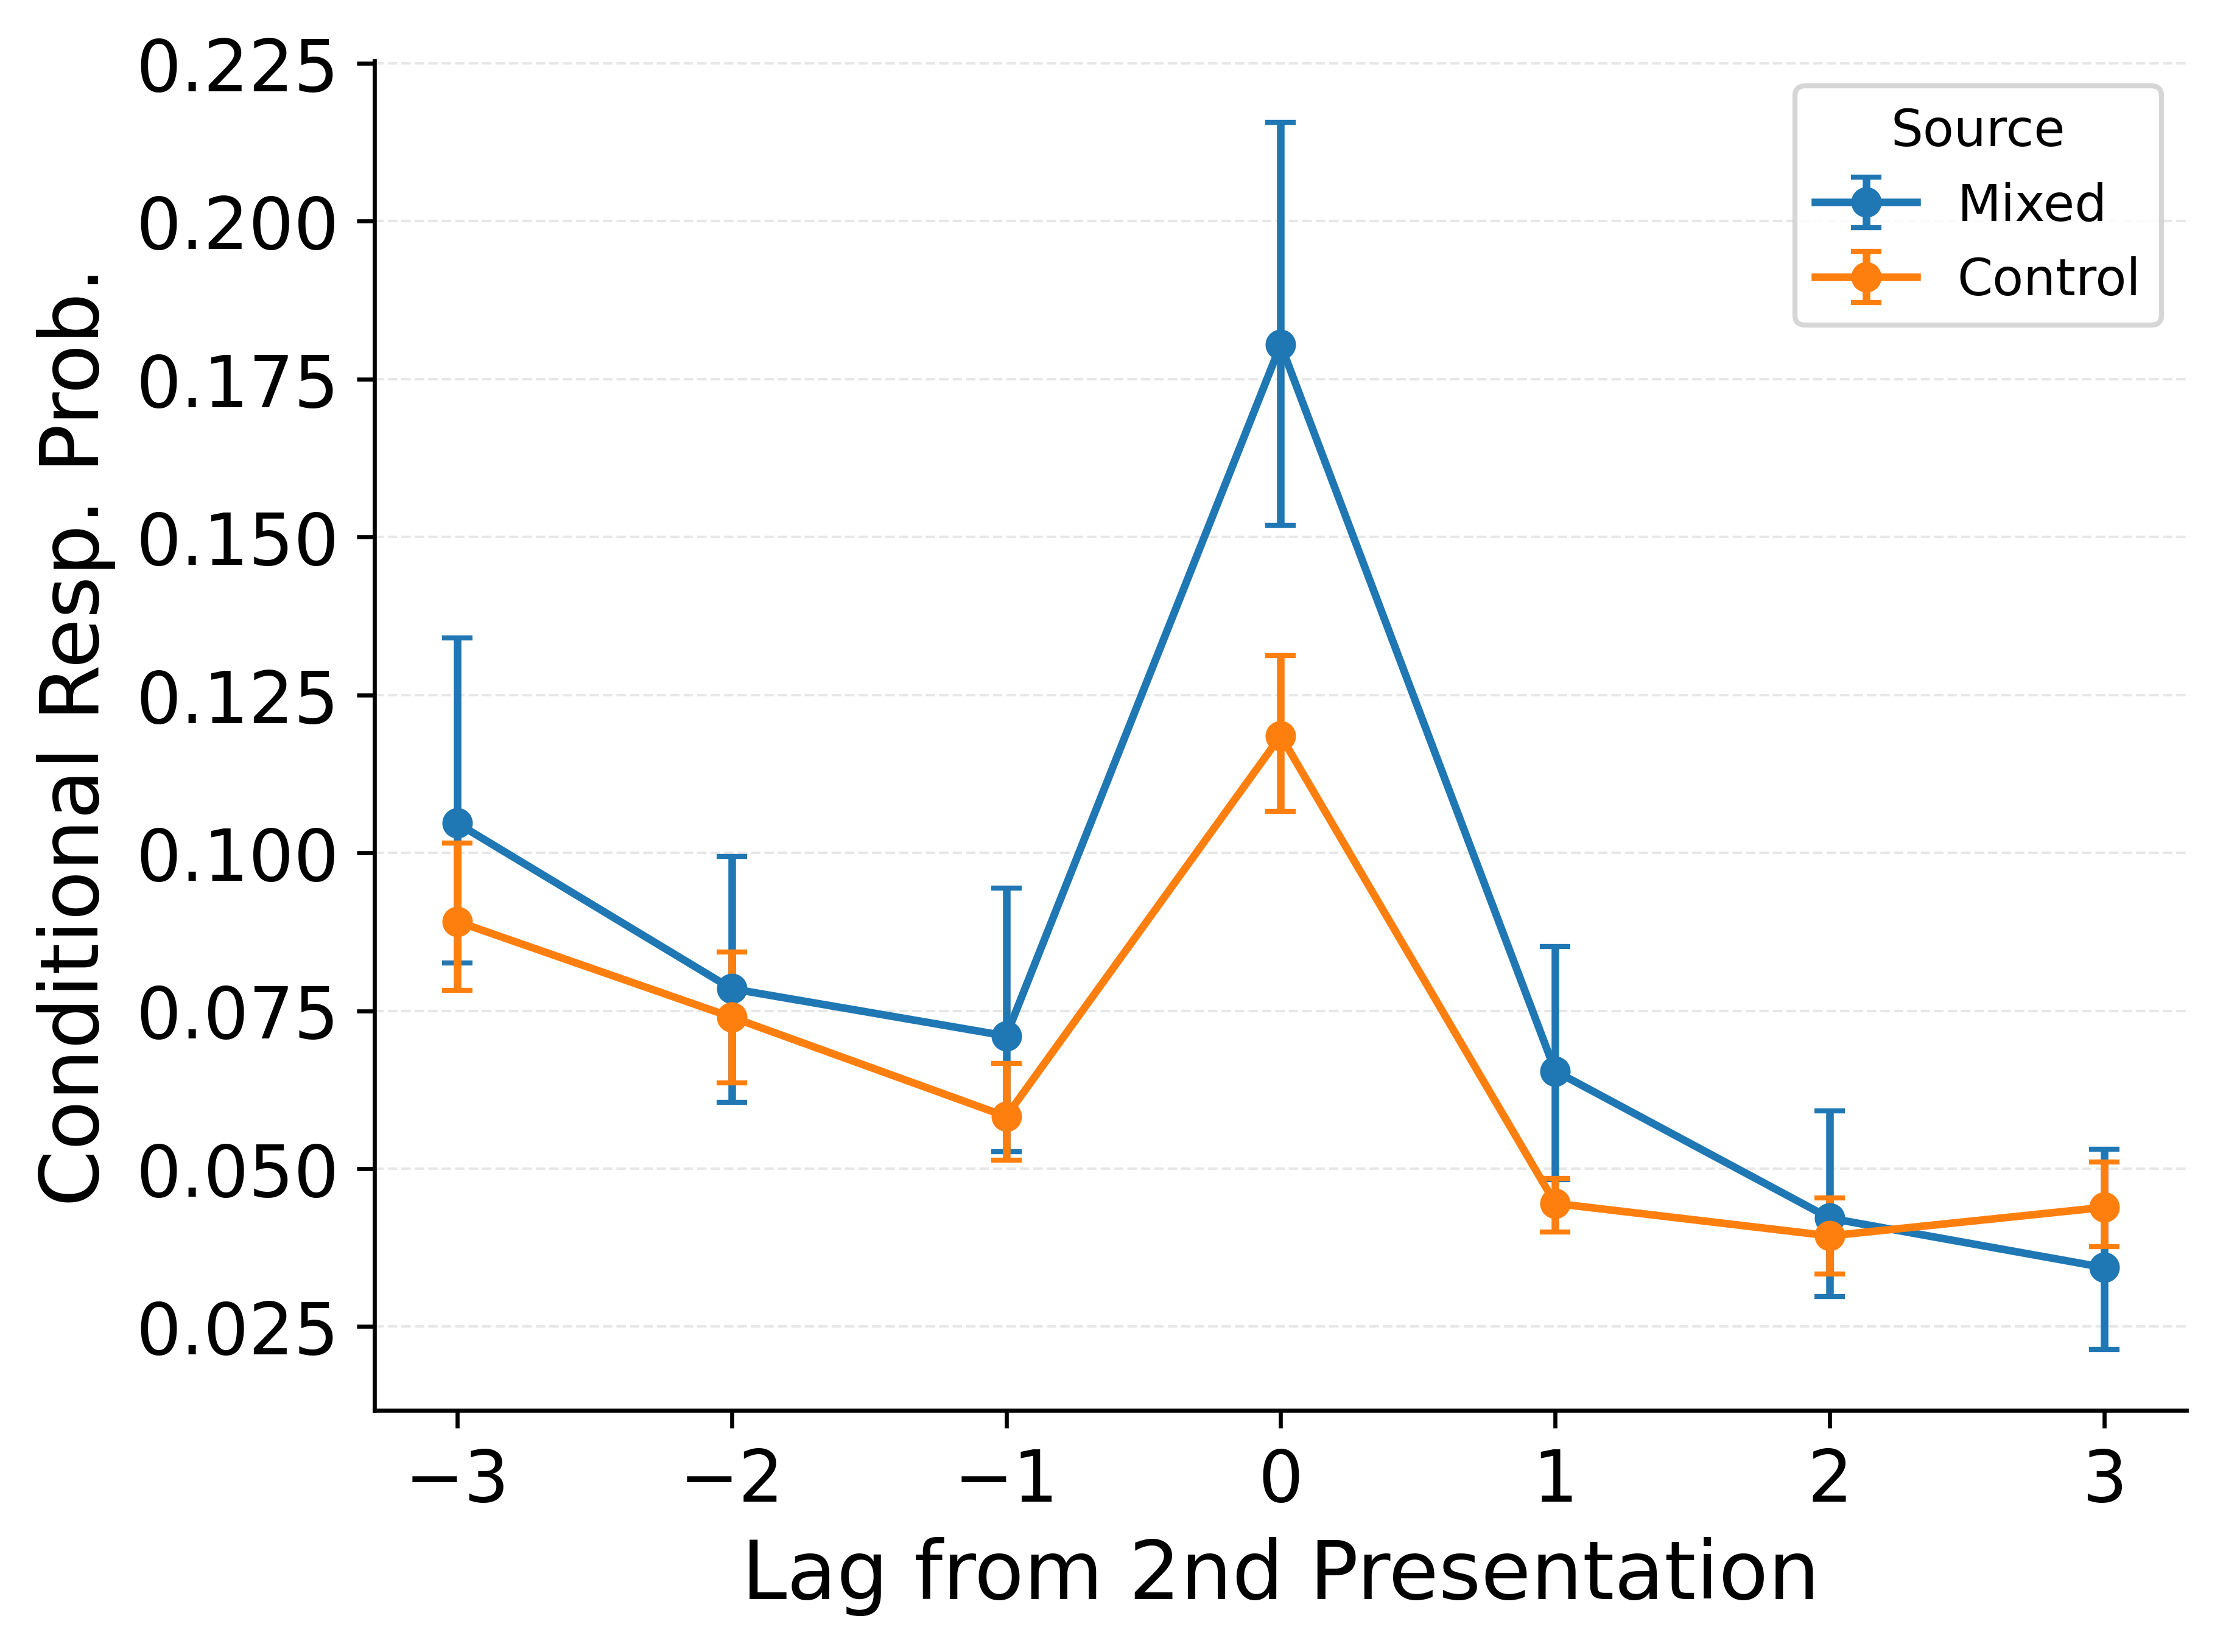
\includegraphics{../../work/thesis/figures/LohnasKahana2014_mixedvscontrolA_data_full_best_of_3_LT4_repneighborcrp_i2j.png}\end{minipage}%
%
\begin{minipage}{0.50\linewidth}
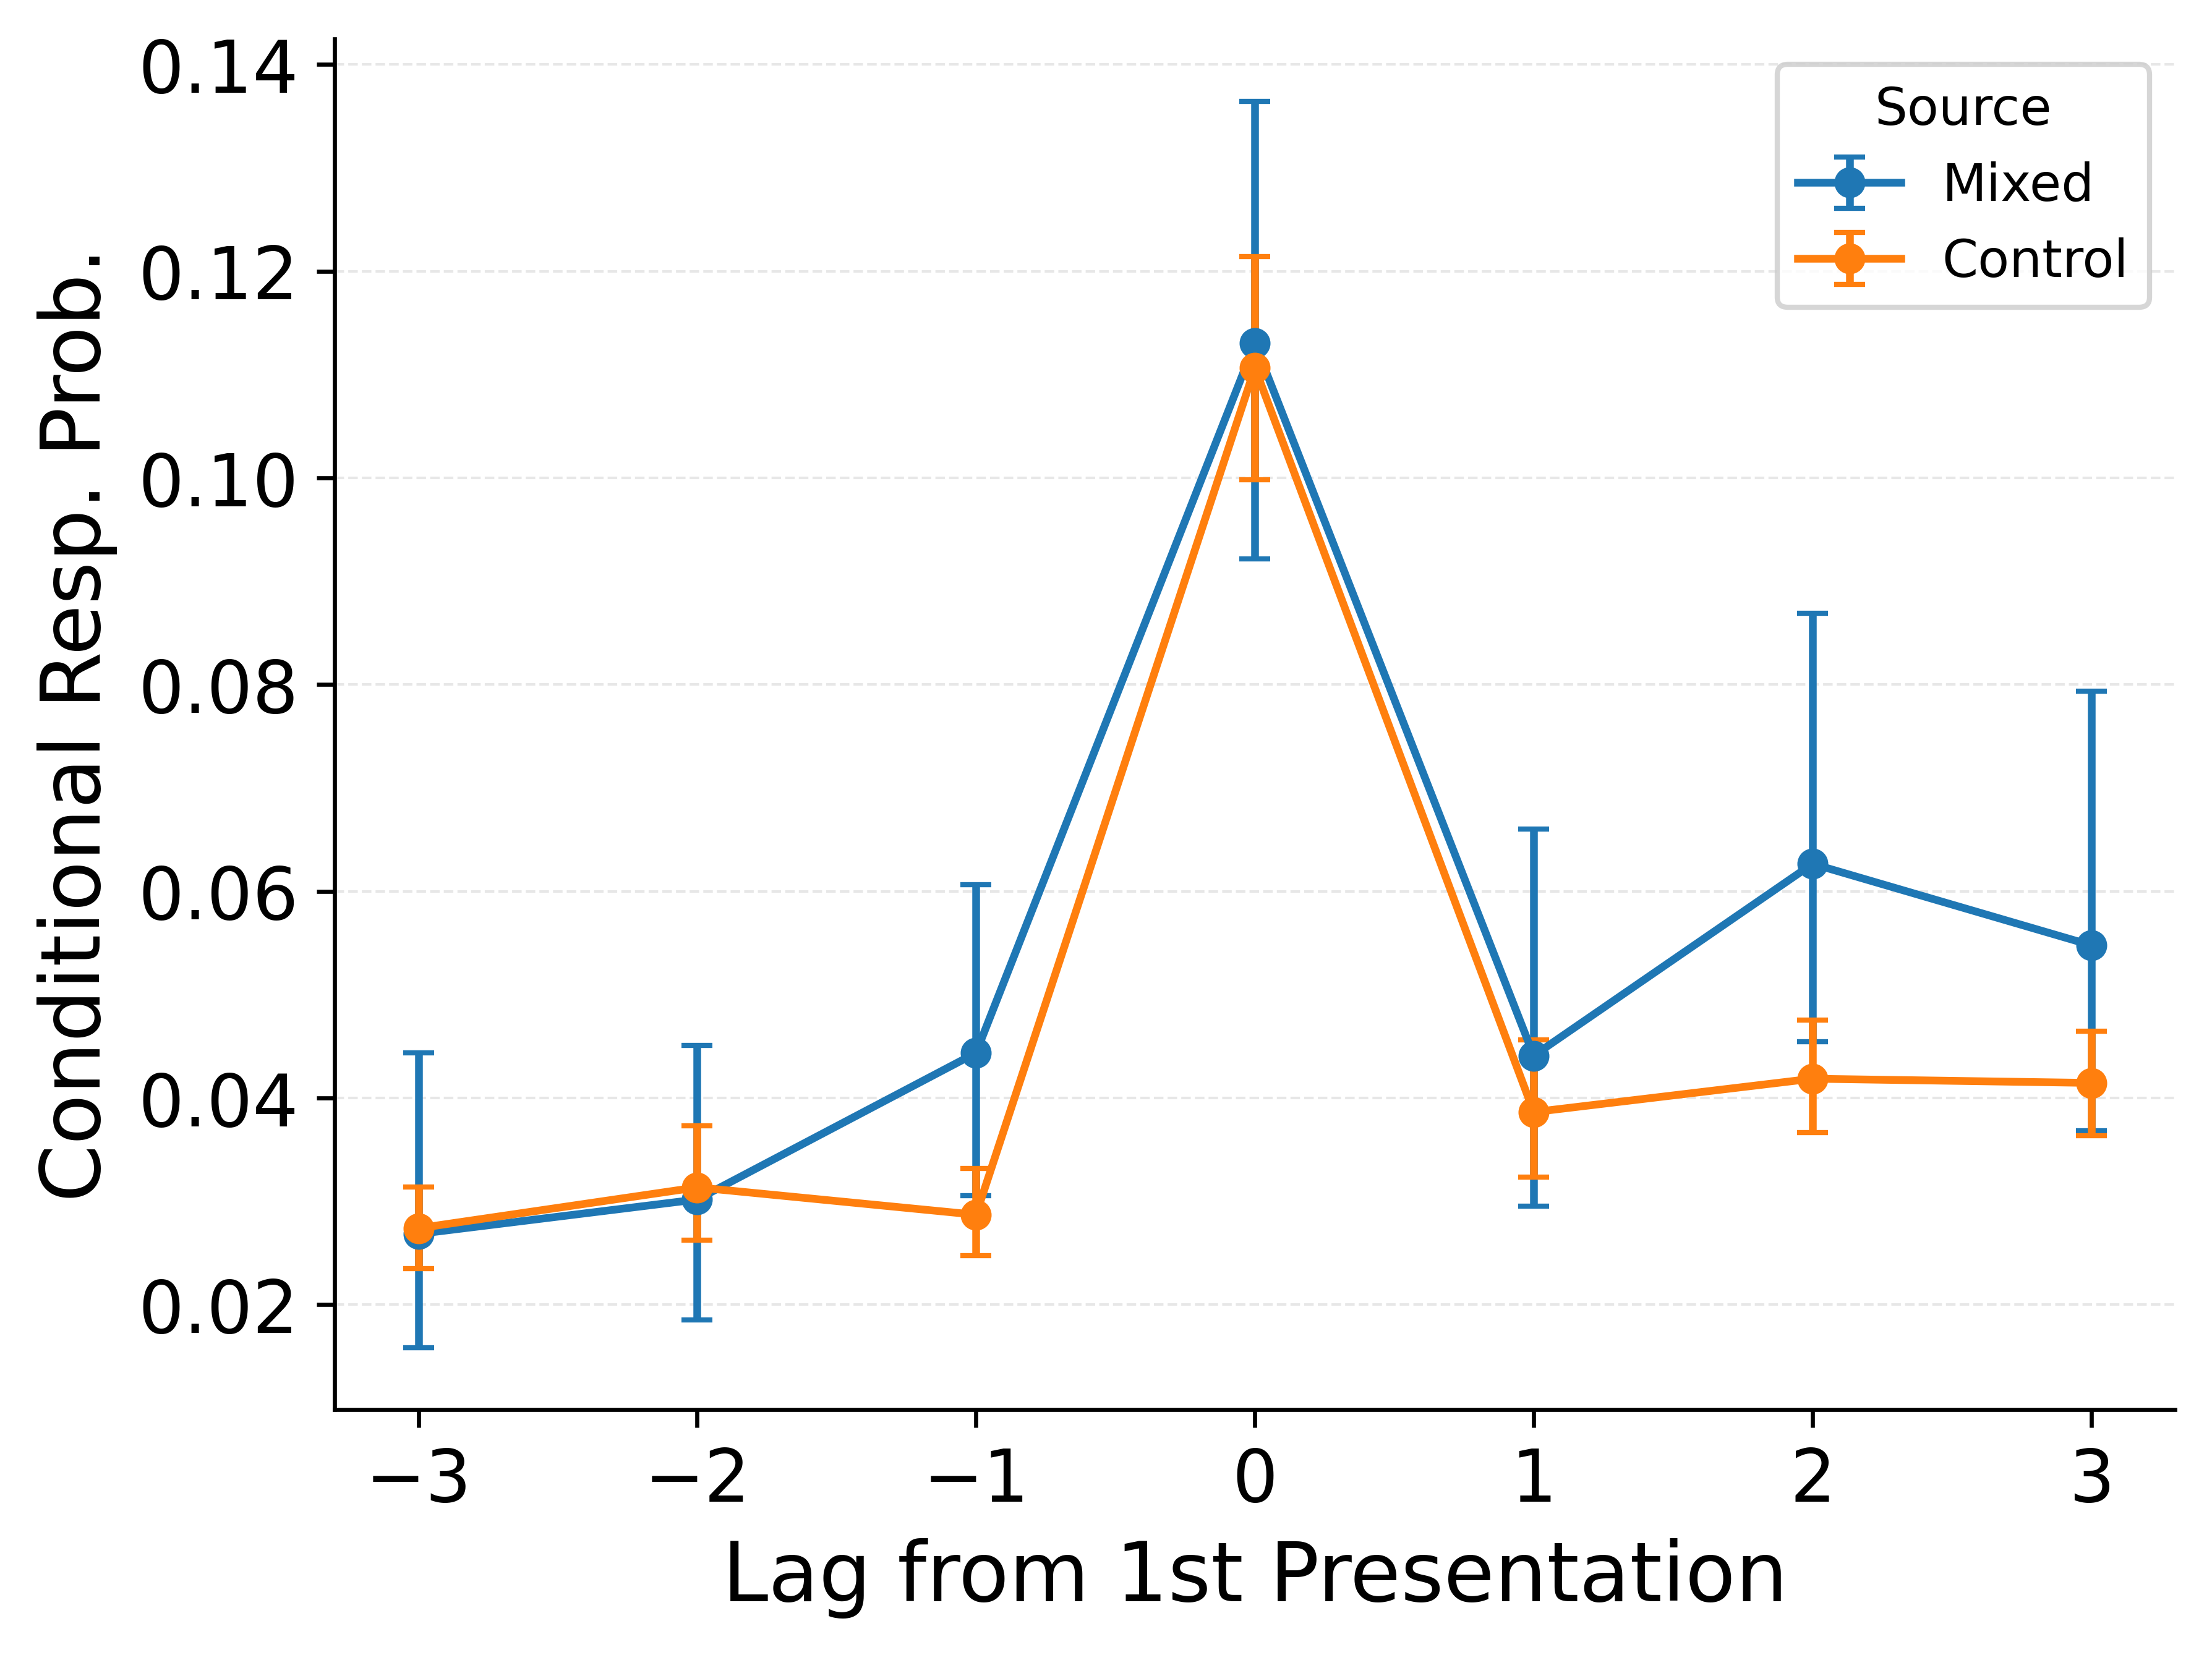
\includegraphics{../../work/thesis/figures/LohnasKahana2014_mixedvscontrolA_data_full_best_of_3_LT4_repneighborcrp_j2i.png}\end{minipage}%
\newline
\begin{minipage}{0.50\linewidth}
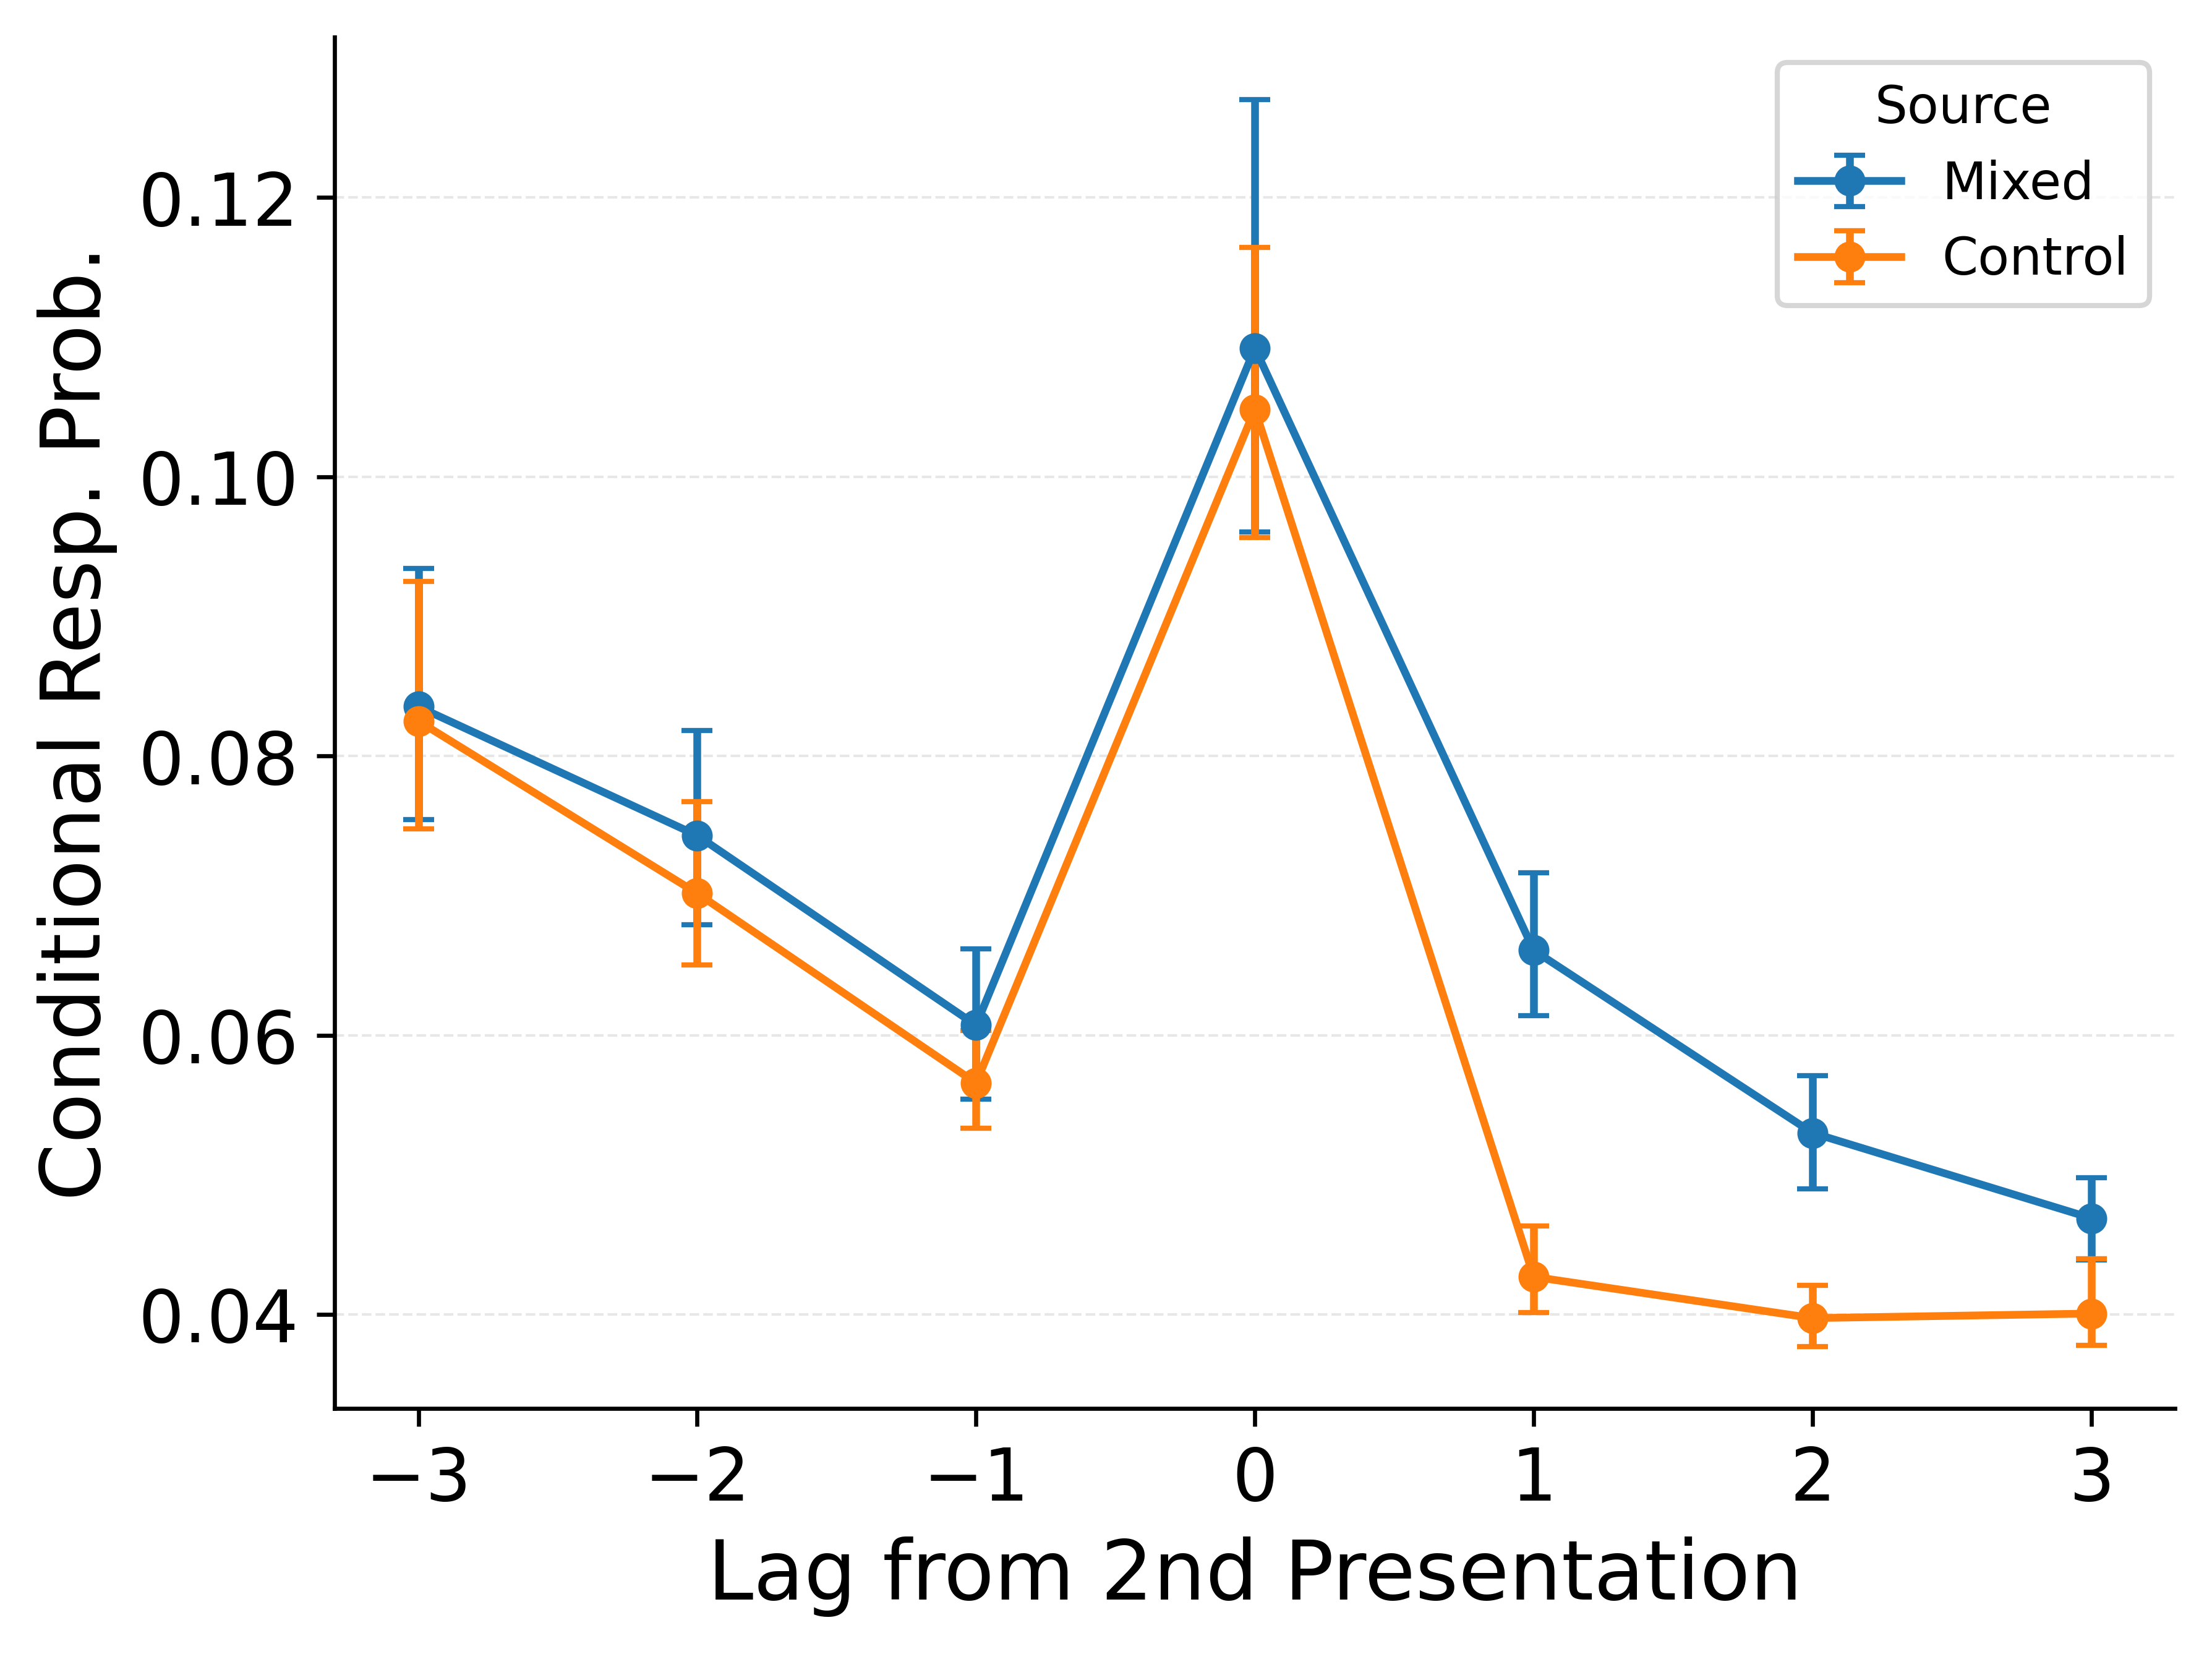
\includegraphics{../../work/thesis/figures/LohnasKahana2014_mixedvscontrolA_WeirdCMR_full_best_of_3_LT4_repneighborcrp_i2j.png}\end{minipage}%
%
\begin{minipage}{0.50\linewidth}
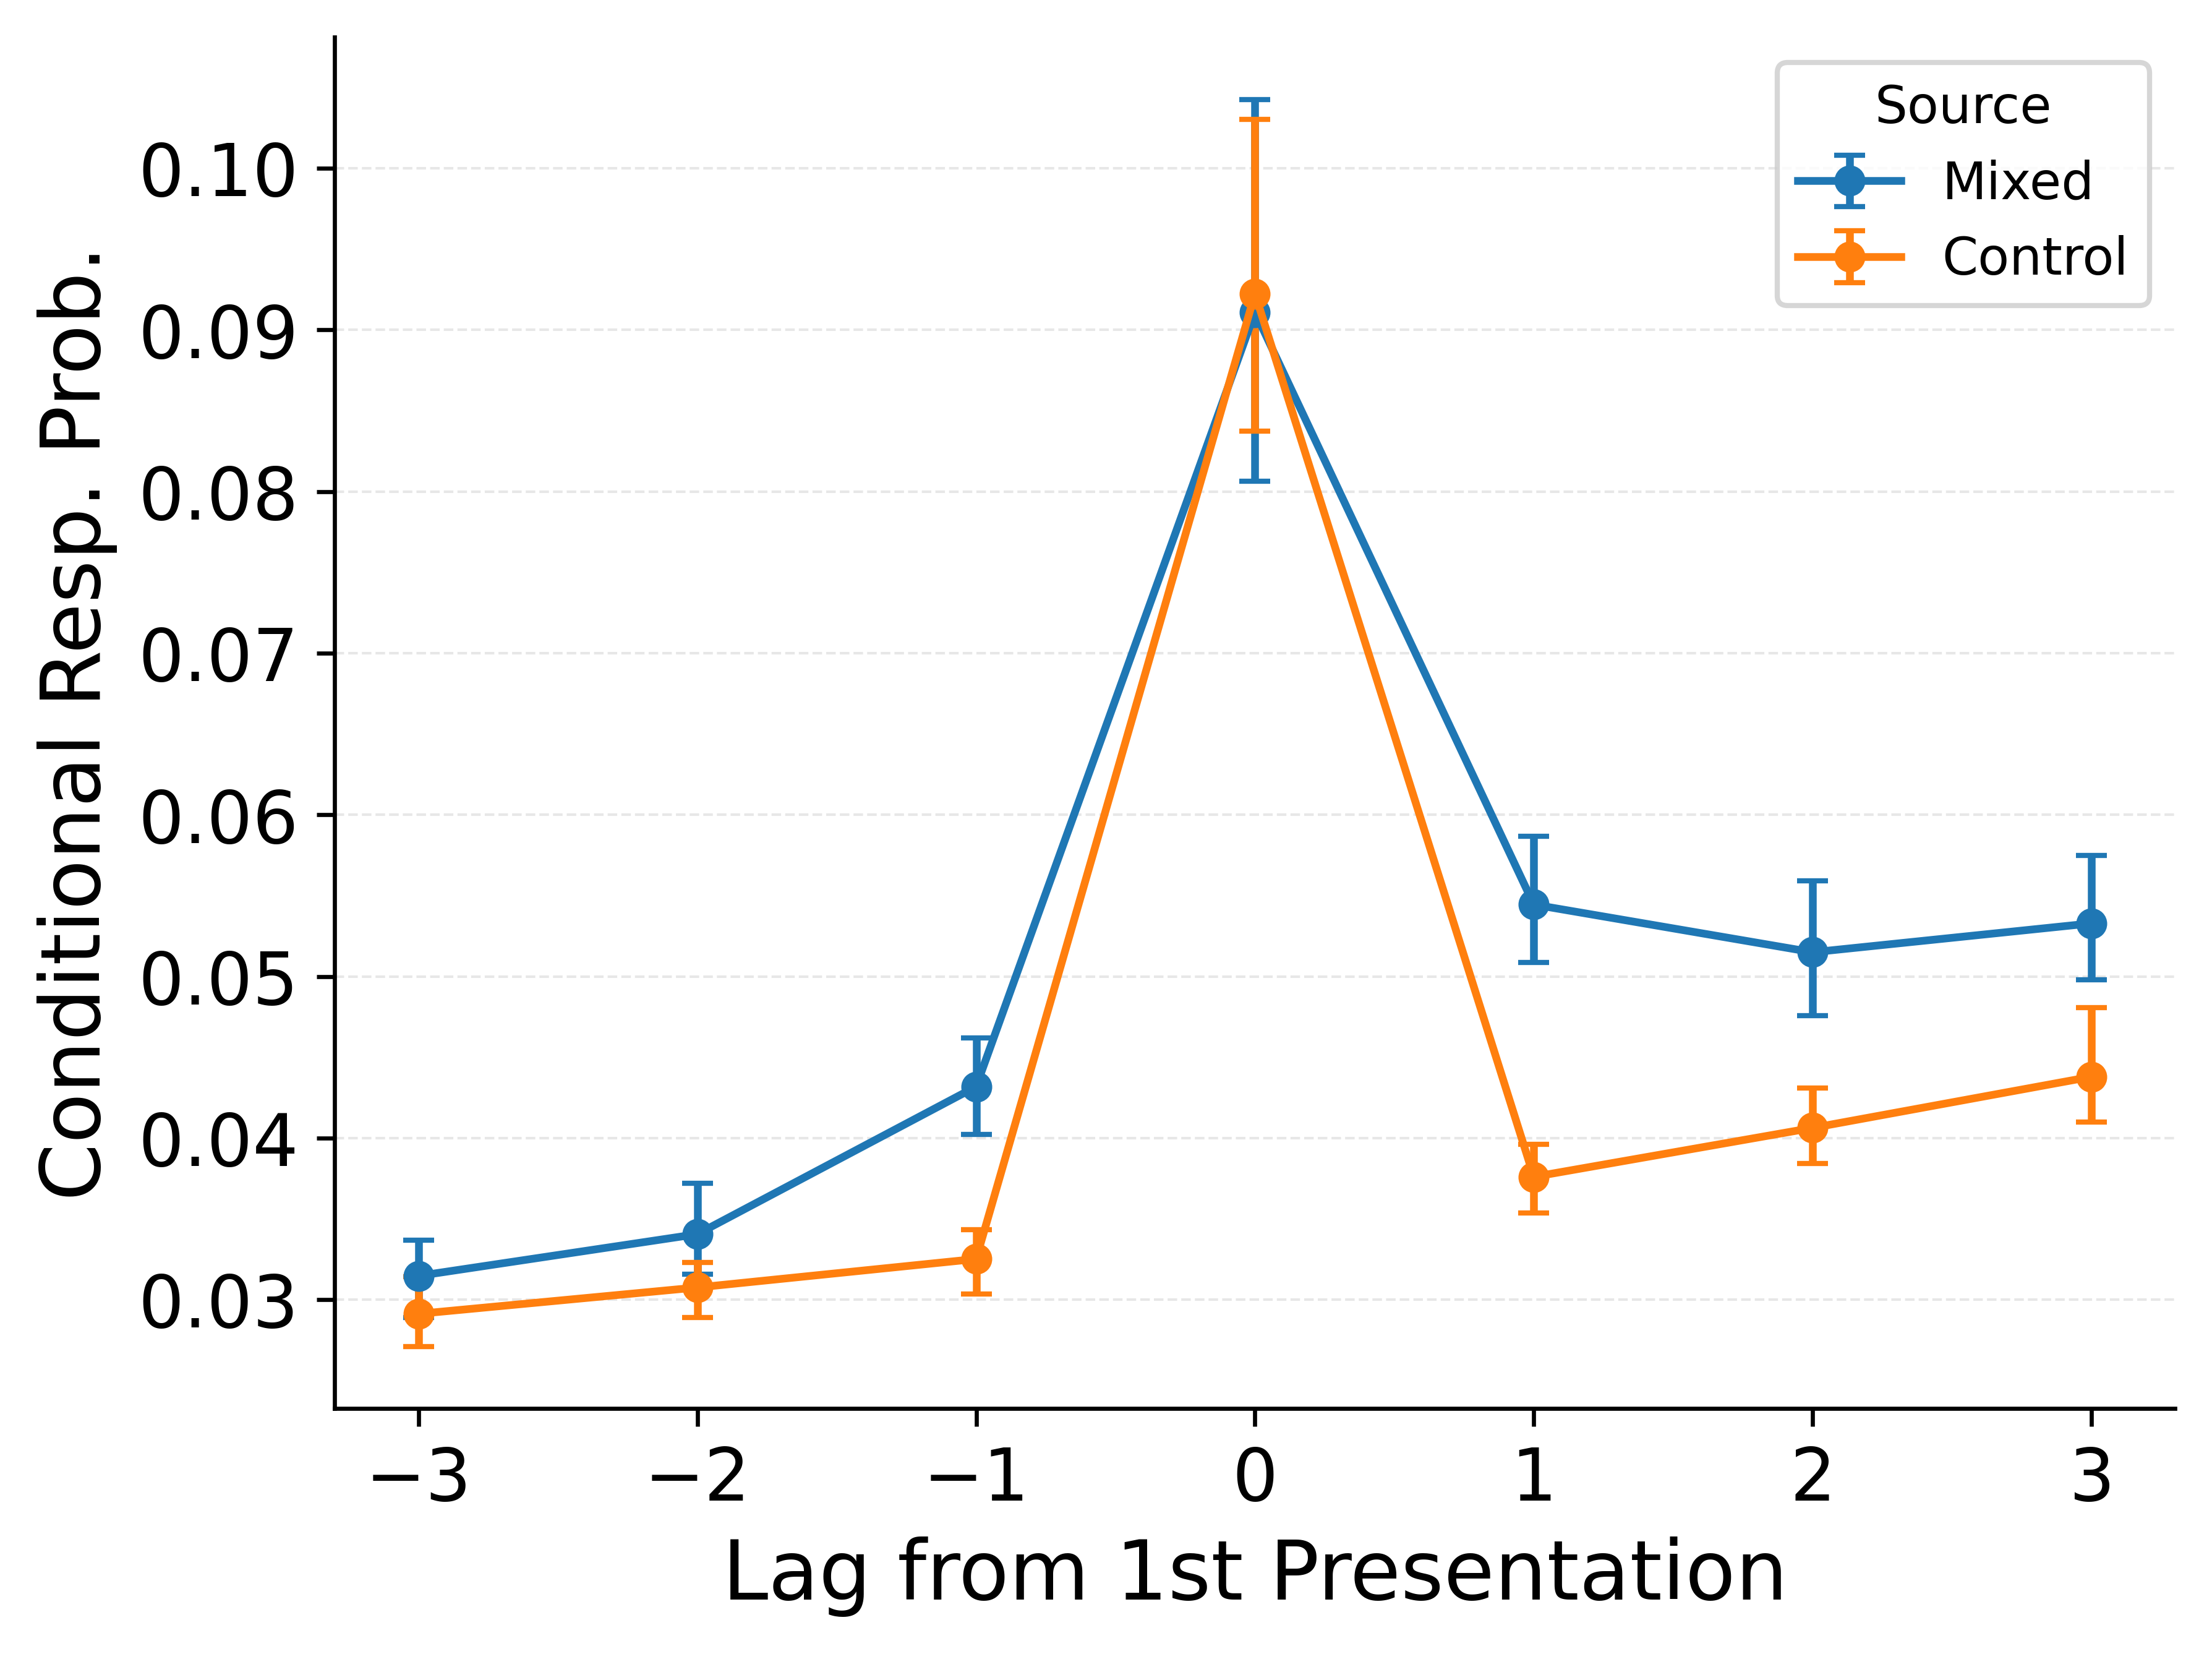
\includegraphics{../../work/thesis/figures/LohnasKahana2014_mixedvscontrolA_WeirdCMR_full_best_of_3_LT4_repneighborcrp_j2i.png}\end{minipage}%

\end{figure}%

\subsection{The Repetition Lag-CRP}\label{the-repetition-lag-crp}

The outgoing repetition lag-CRP quantifies how a recalled repeater cues
subsequent recall from each occurrence's neighborhood
(Figure~\ref{fig-repetition_lag_crp}). In the data, transitions from the
repeated item preferentially target neighbors of the item's first study
position instead of neighbors of the second. In particular, the \(+1\)
bin from the first-centered cue exceeds the \(+1\) bin from the
second-centered cue, and this separation is larger than in the
position-matched baseline.

Our simulations of standard CMR (bottom row of
Figure~\ref{fig-repetition_lag_crp}) demonstrate the opposite pattern,
consistent with its prediction of cross-occurrence associative
interference. CMR makes it difficult to cue neighbors of an item's first
occurrence without also cueing neighbors of the second occurrence. Thus
for recalled items presented at study positions \(i\) and \(j\), CMR
predicts relatively balanced transition rates to positions \(i{+}1\) and
\(j{+}1\) relative to the baseline. This conflict isolates the problem:
when the repeater is recalled, the model's item-based reinstatement
routes through a composite of contexts, whereas people's recalls behave
as if a single occurrence's context is (selectively) reinstated.

\begin{figure}

\caption{\label{fig-repetition_lag_crp}Repetition lag-CRP (outgoing):
data vs CMR. Top row (data): mixed lists (left) and matched-control
baseline (right), each showing two centered curves (first-centered vs
second-centered). Bottom row (CMR): same for simulations. In data,
separation (e.g., +1 bin) favors the first-occurrence neighborhood and
is larger than in baseline; CMR predicts reduced separation (balanced
access), consistent with blending.}

\begin{minipage}{0.50\linewidth}
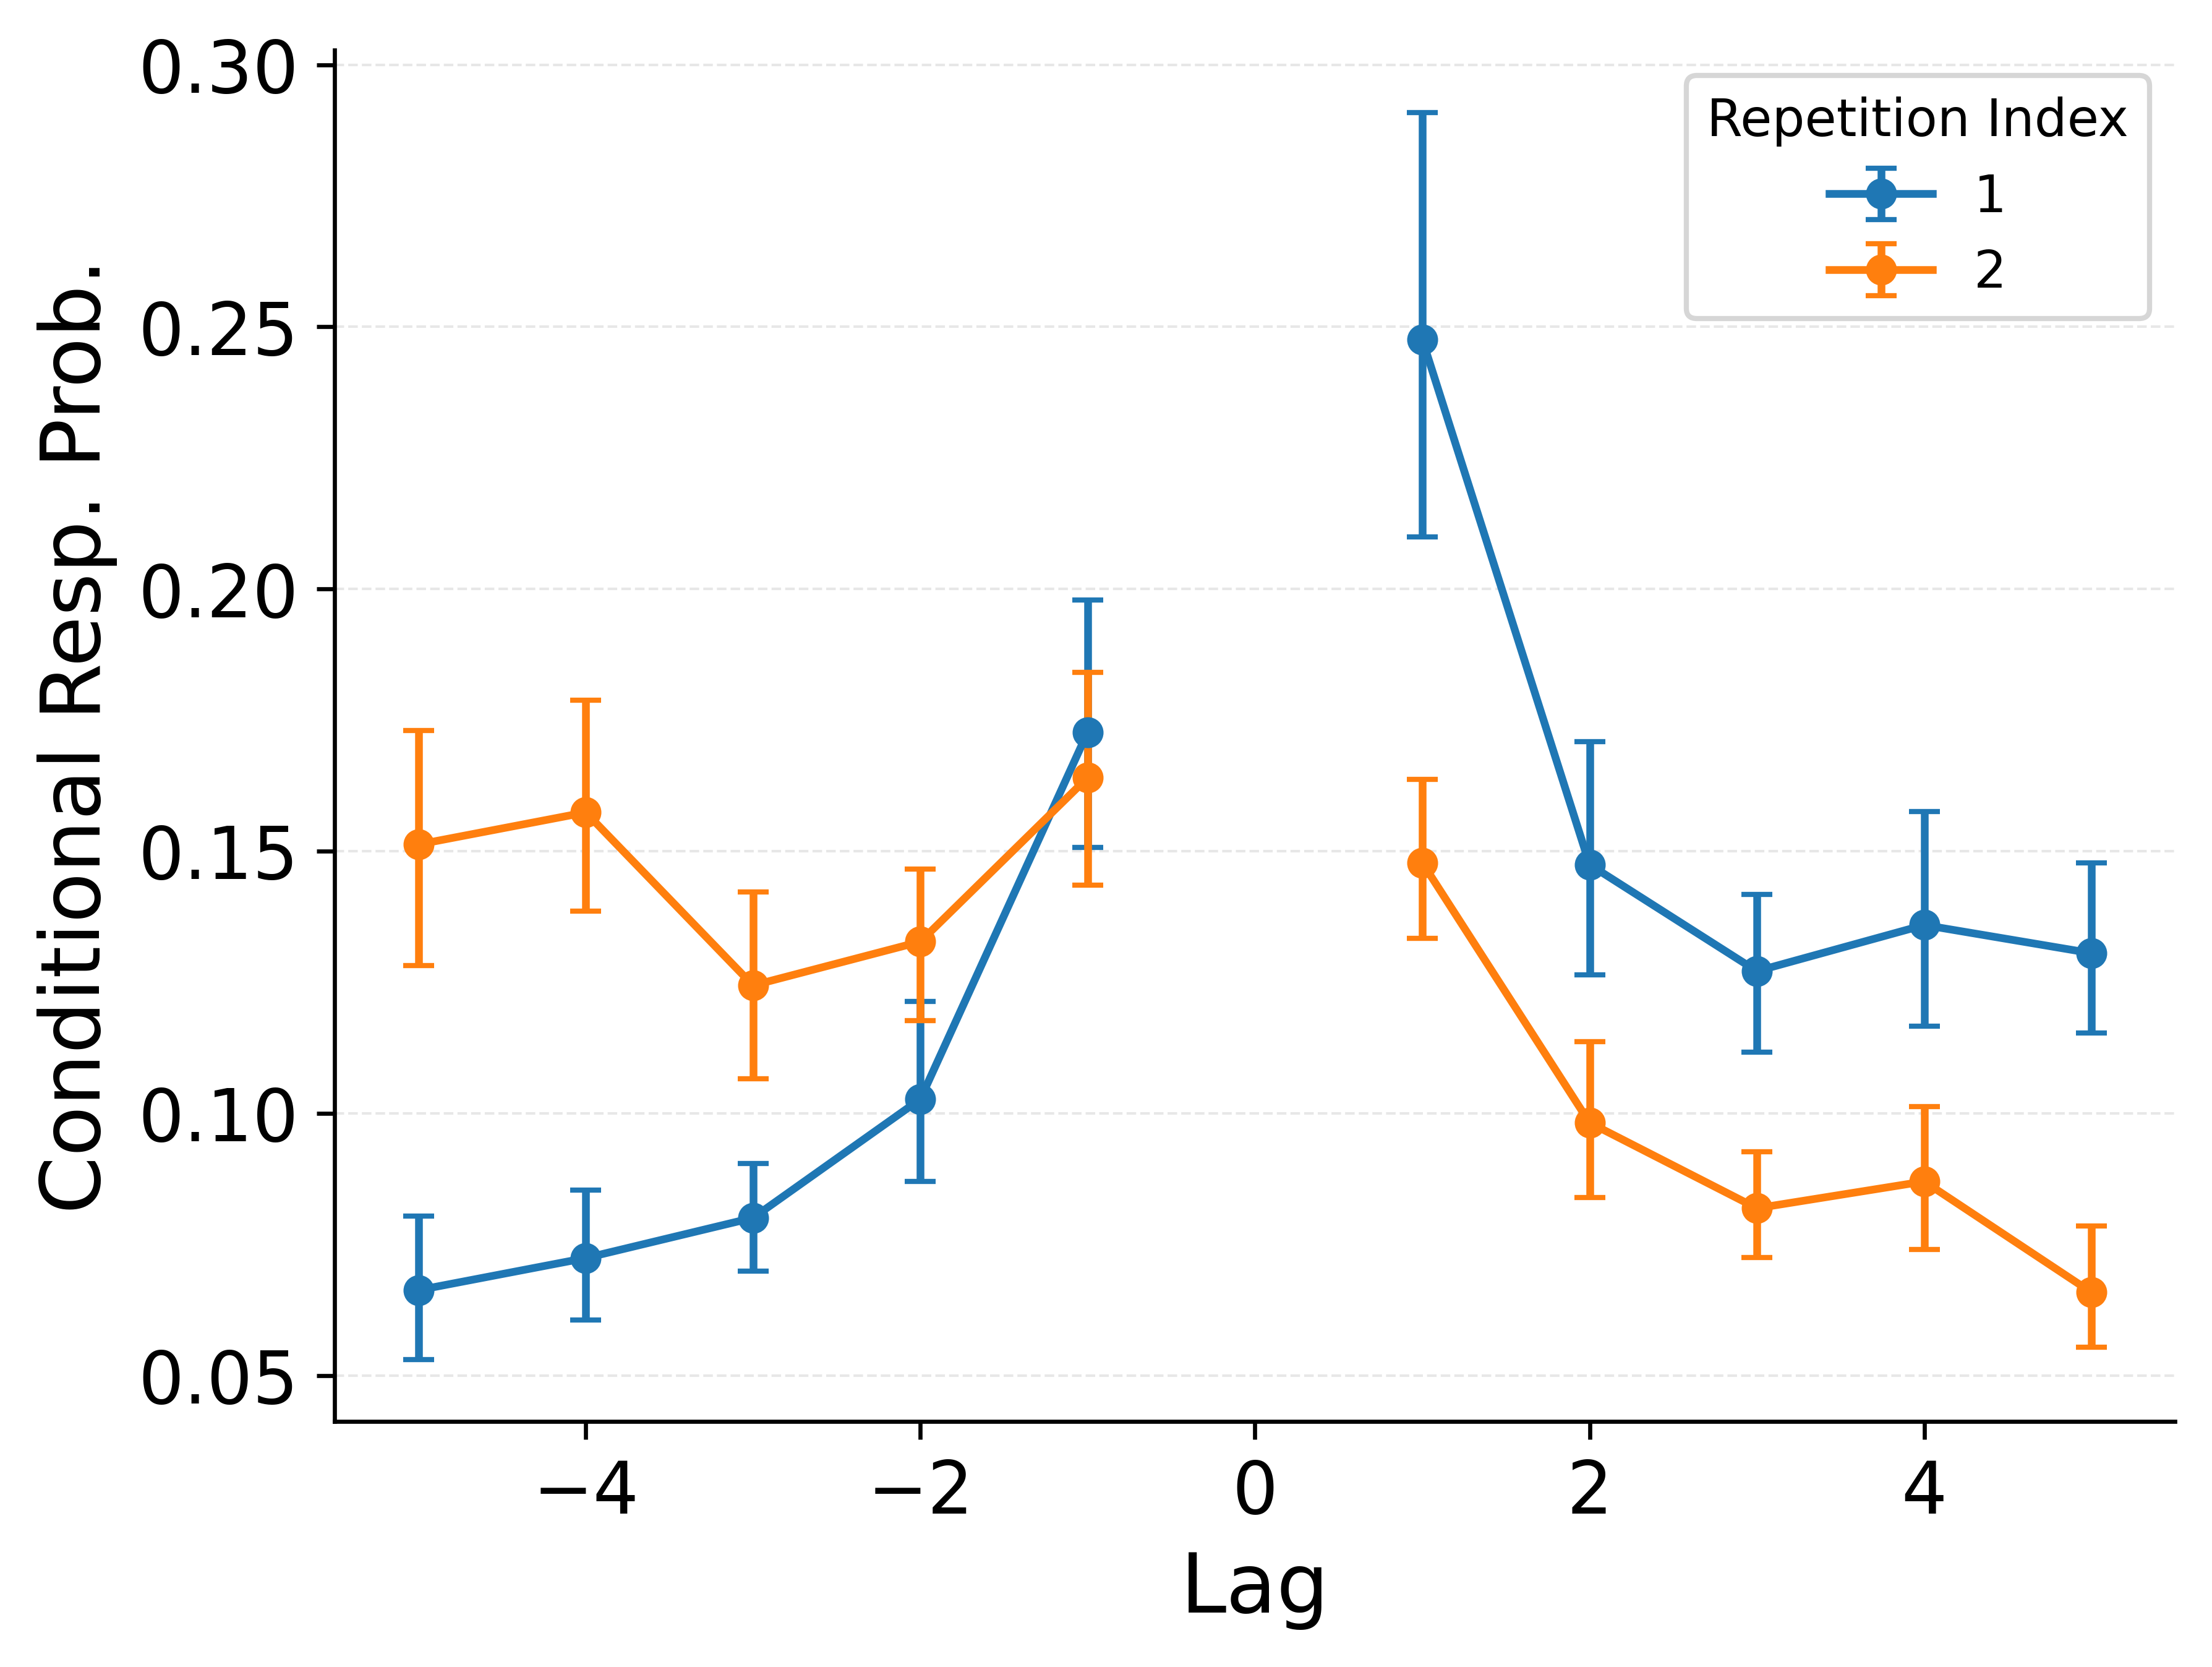
\includegraphics{../../work/thesis/figures/RepeatedRecallsLohnasKahana2014_mixed_data_full_best_of_3_LT34_rep_crp.png}\end{minipage}%
%
\begin{minipage}{0.50\linewidth}
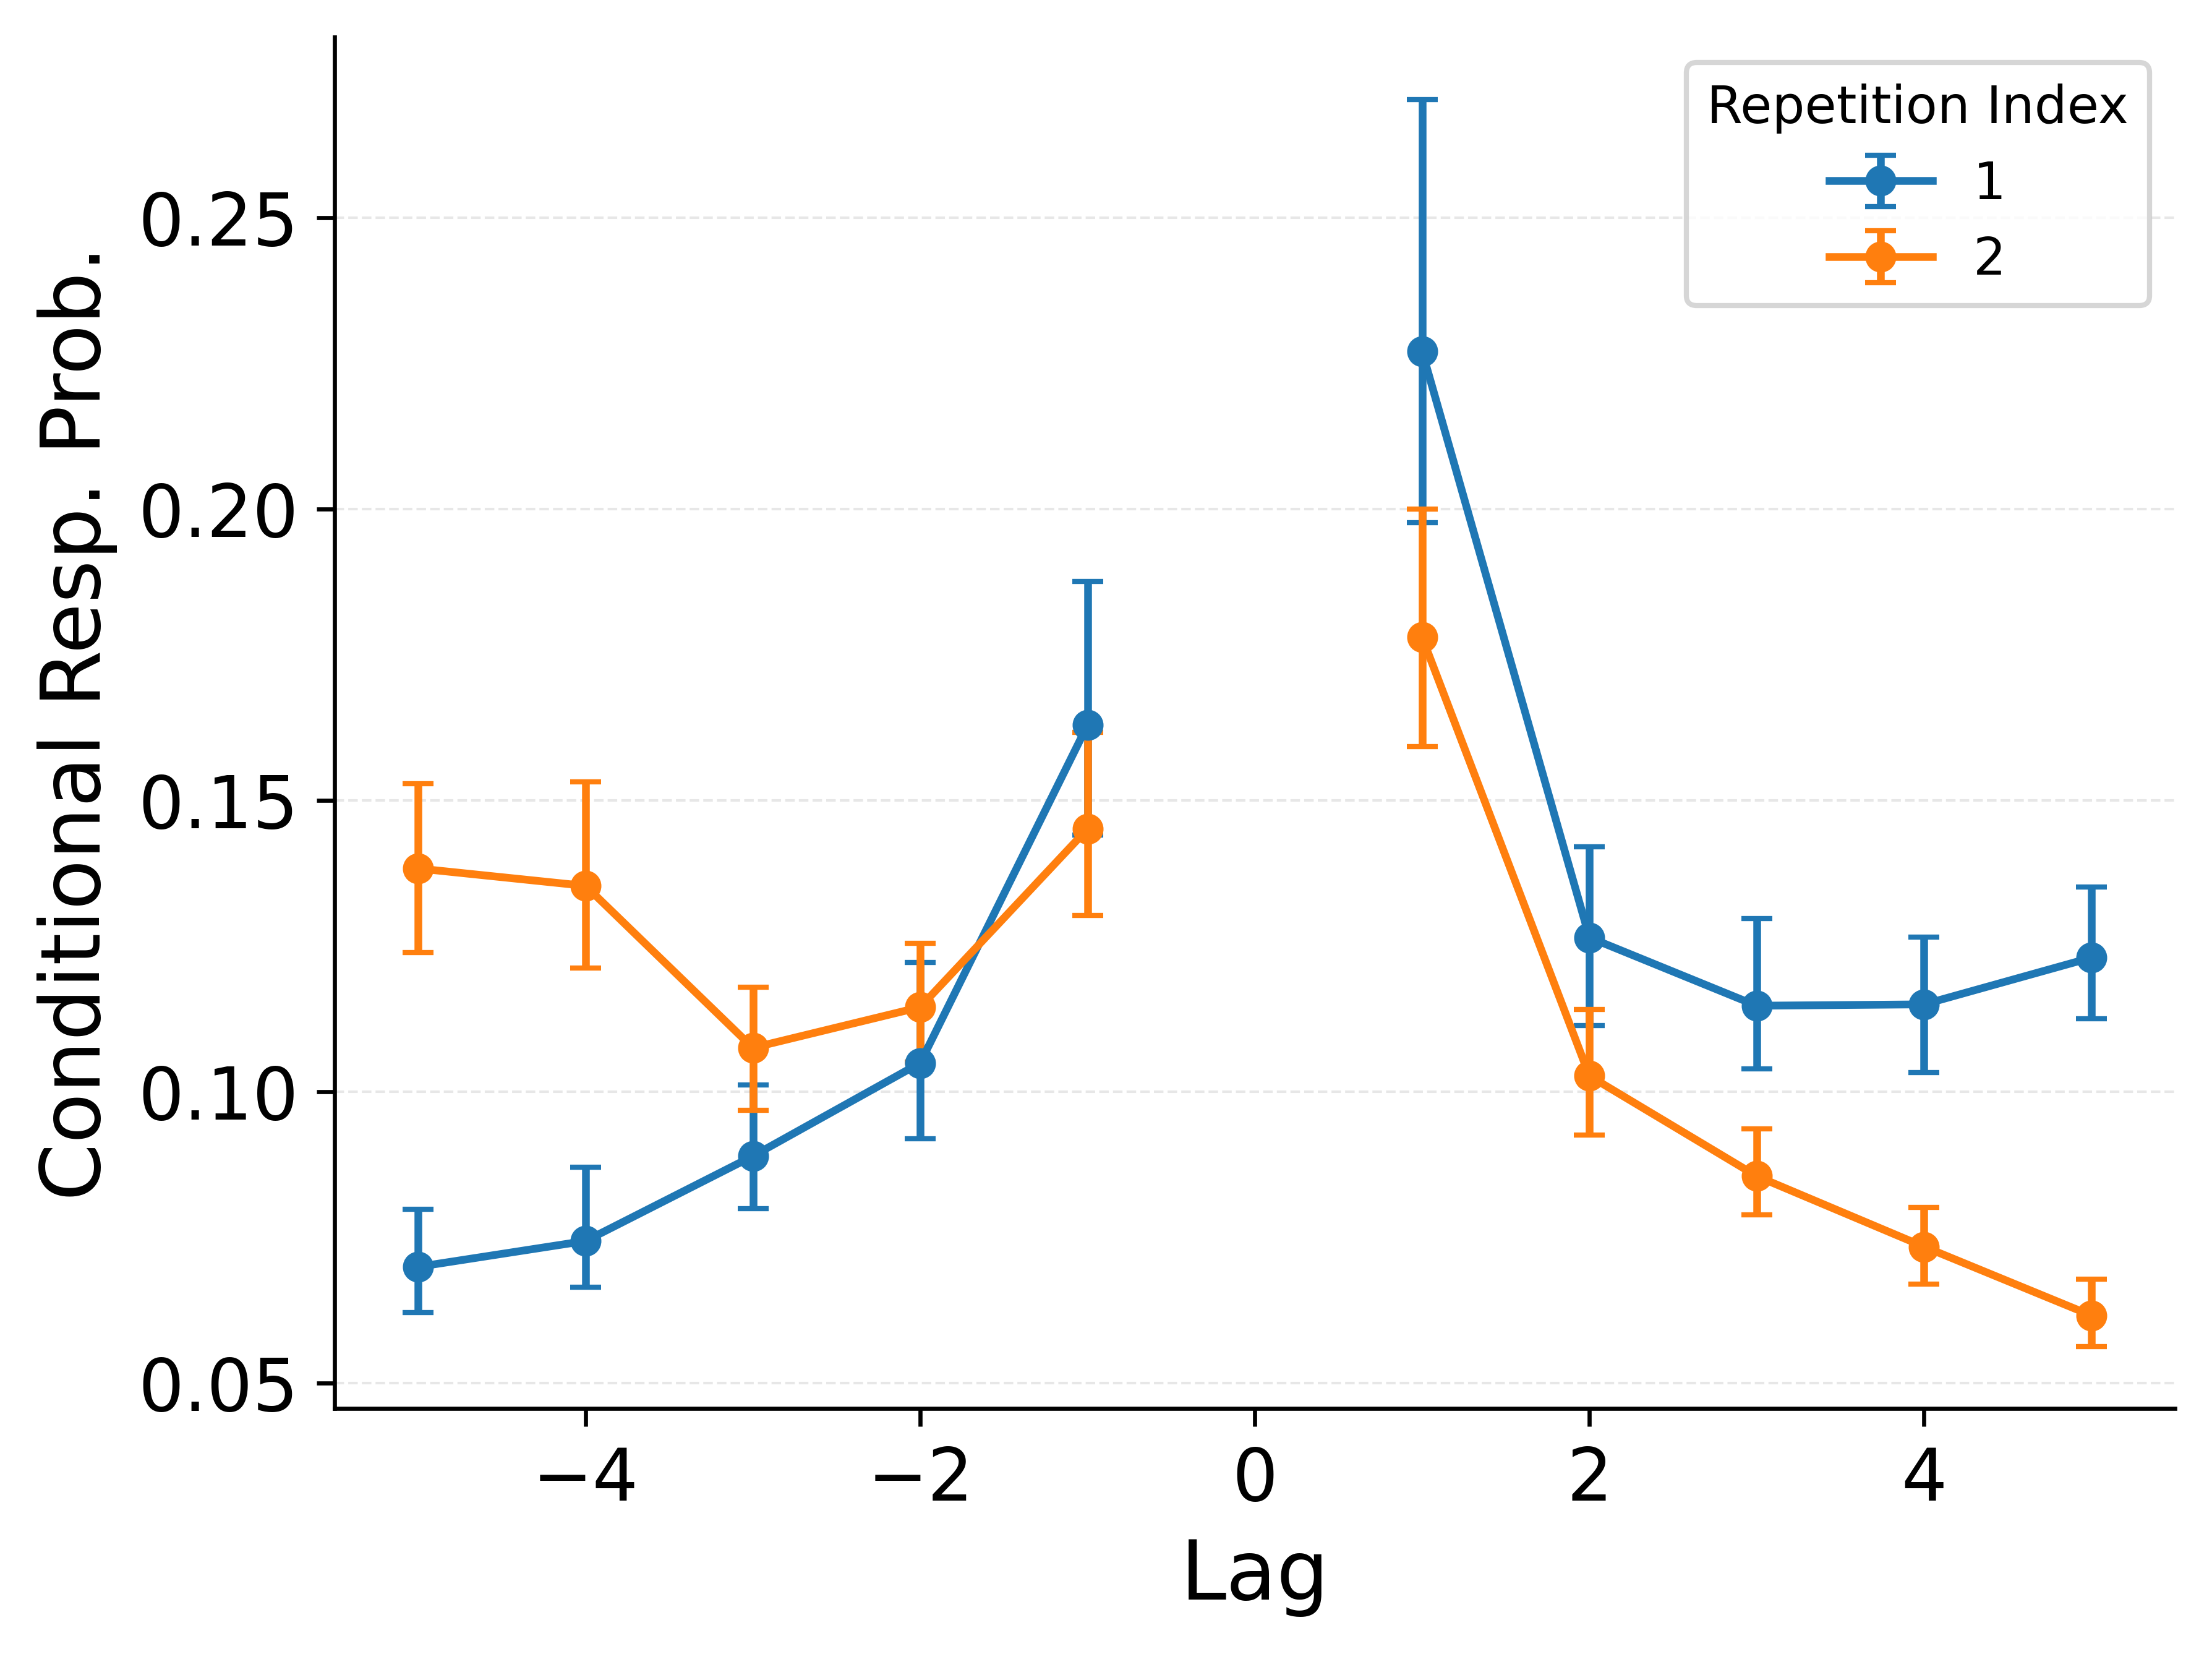
\includegraphics{../../work/thesis/figures/RepeatedRecallsLohnasKahana2014_control_data_full_best_of_3_LT34_rep_crp.png}\end{minipage}%
\newline
\begin{minipage}{0.50\linewidth}
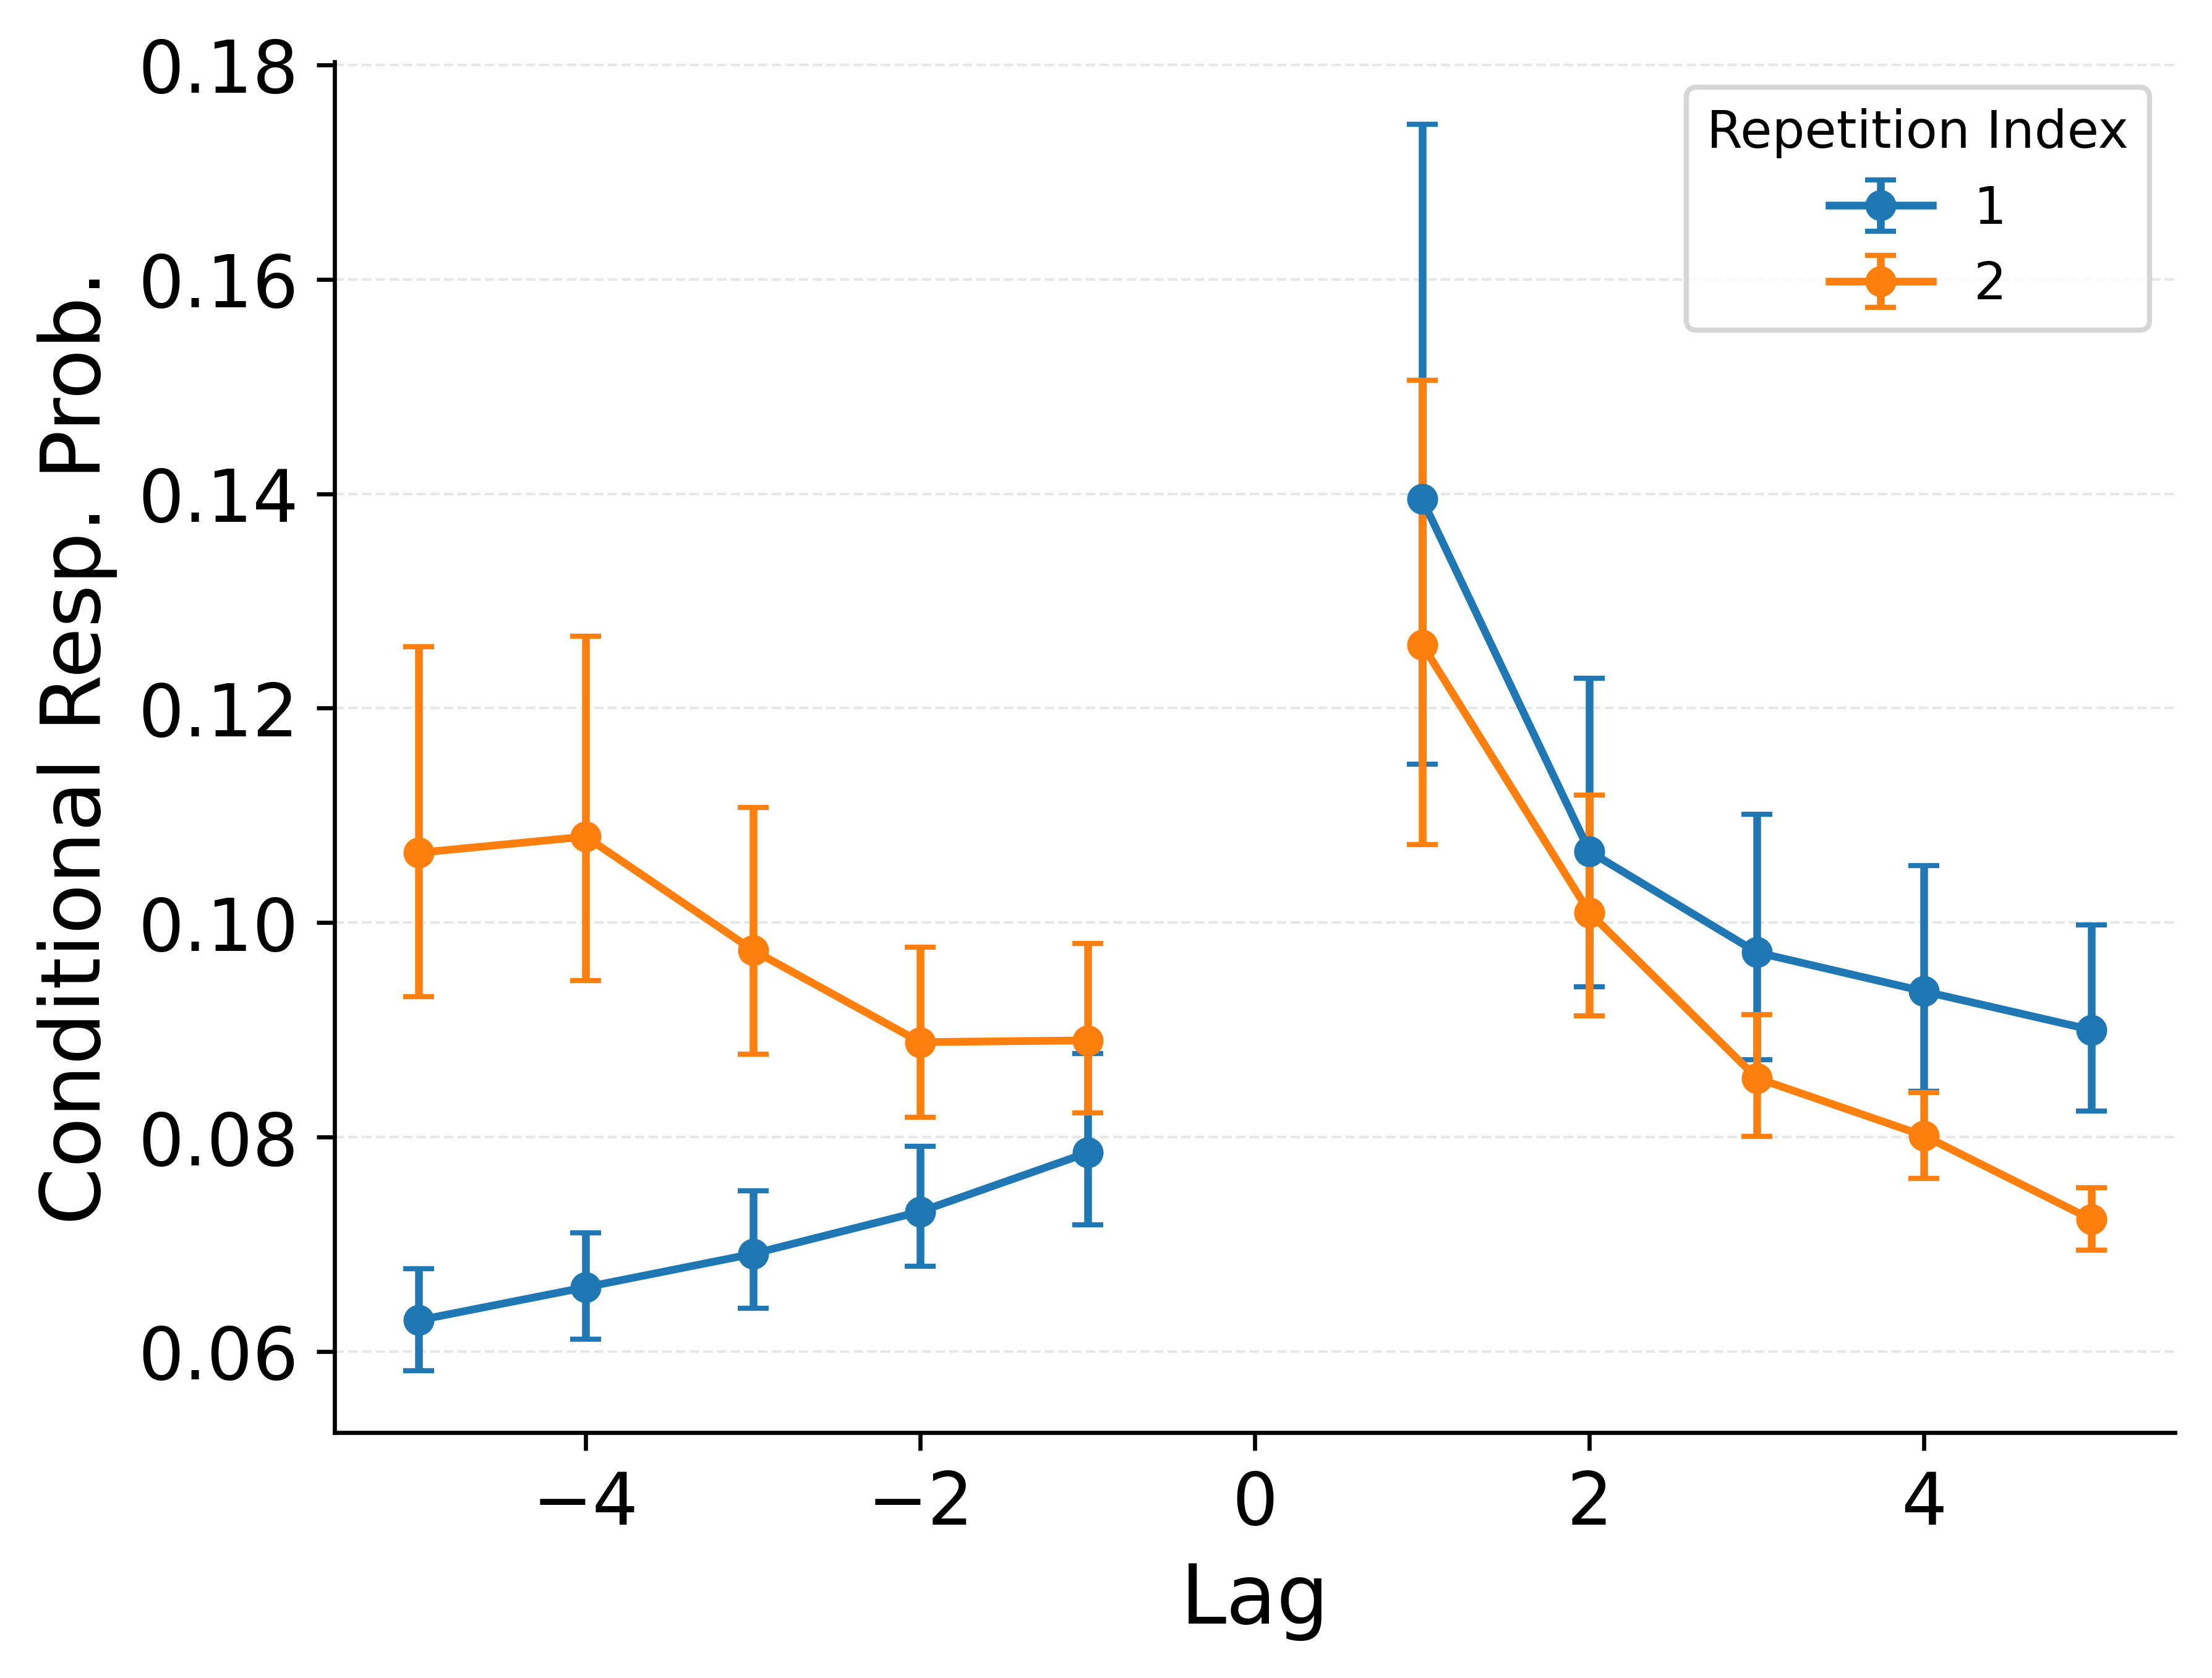
\includegraphics{../../work/thesis/figures/RepeatedRecallsLohnasKahana2014_mixed_WeirdCMR_full_best_of_3_LT34_rep_crp.png}\end{minipage}%
%
\begin{minipage}{0.50\linewidth}
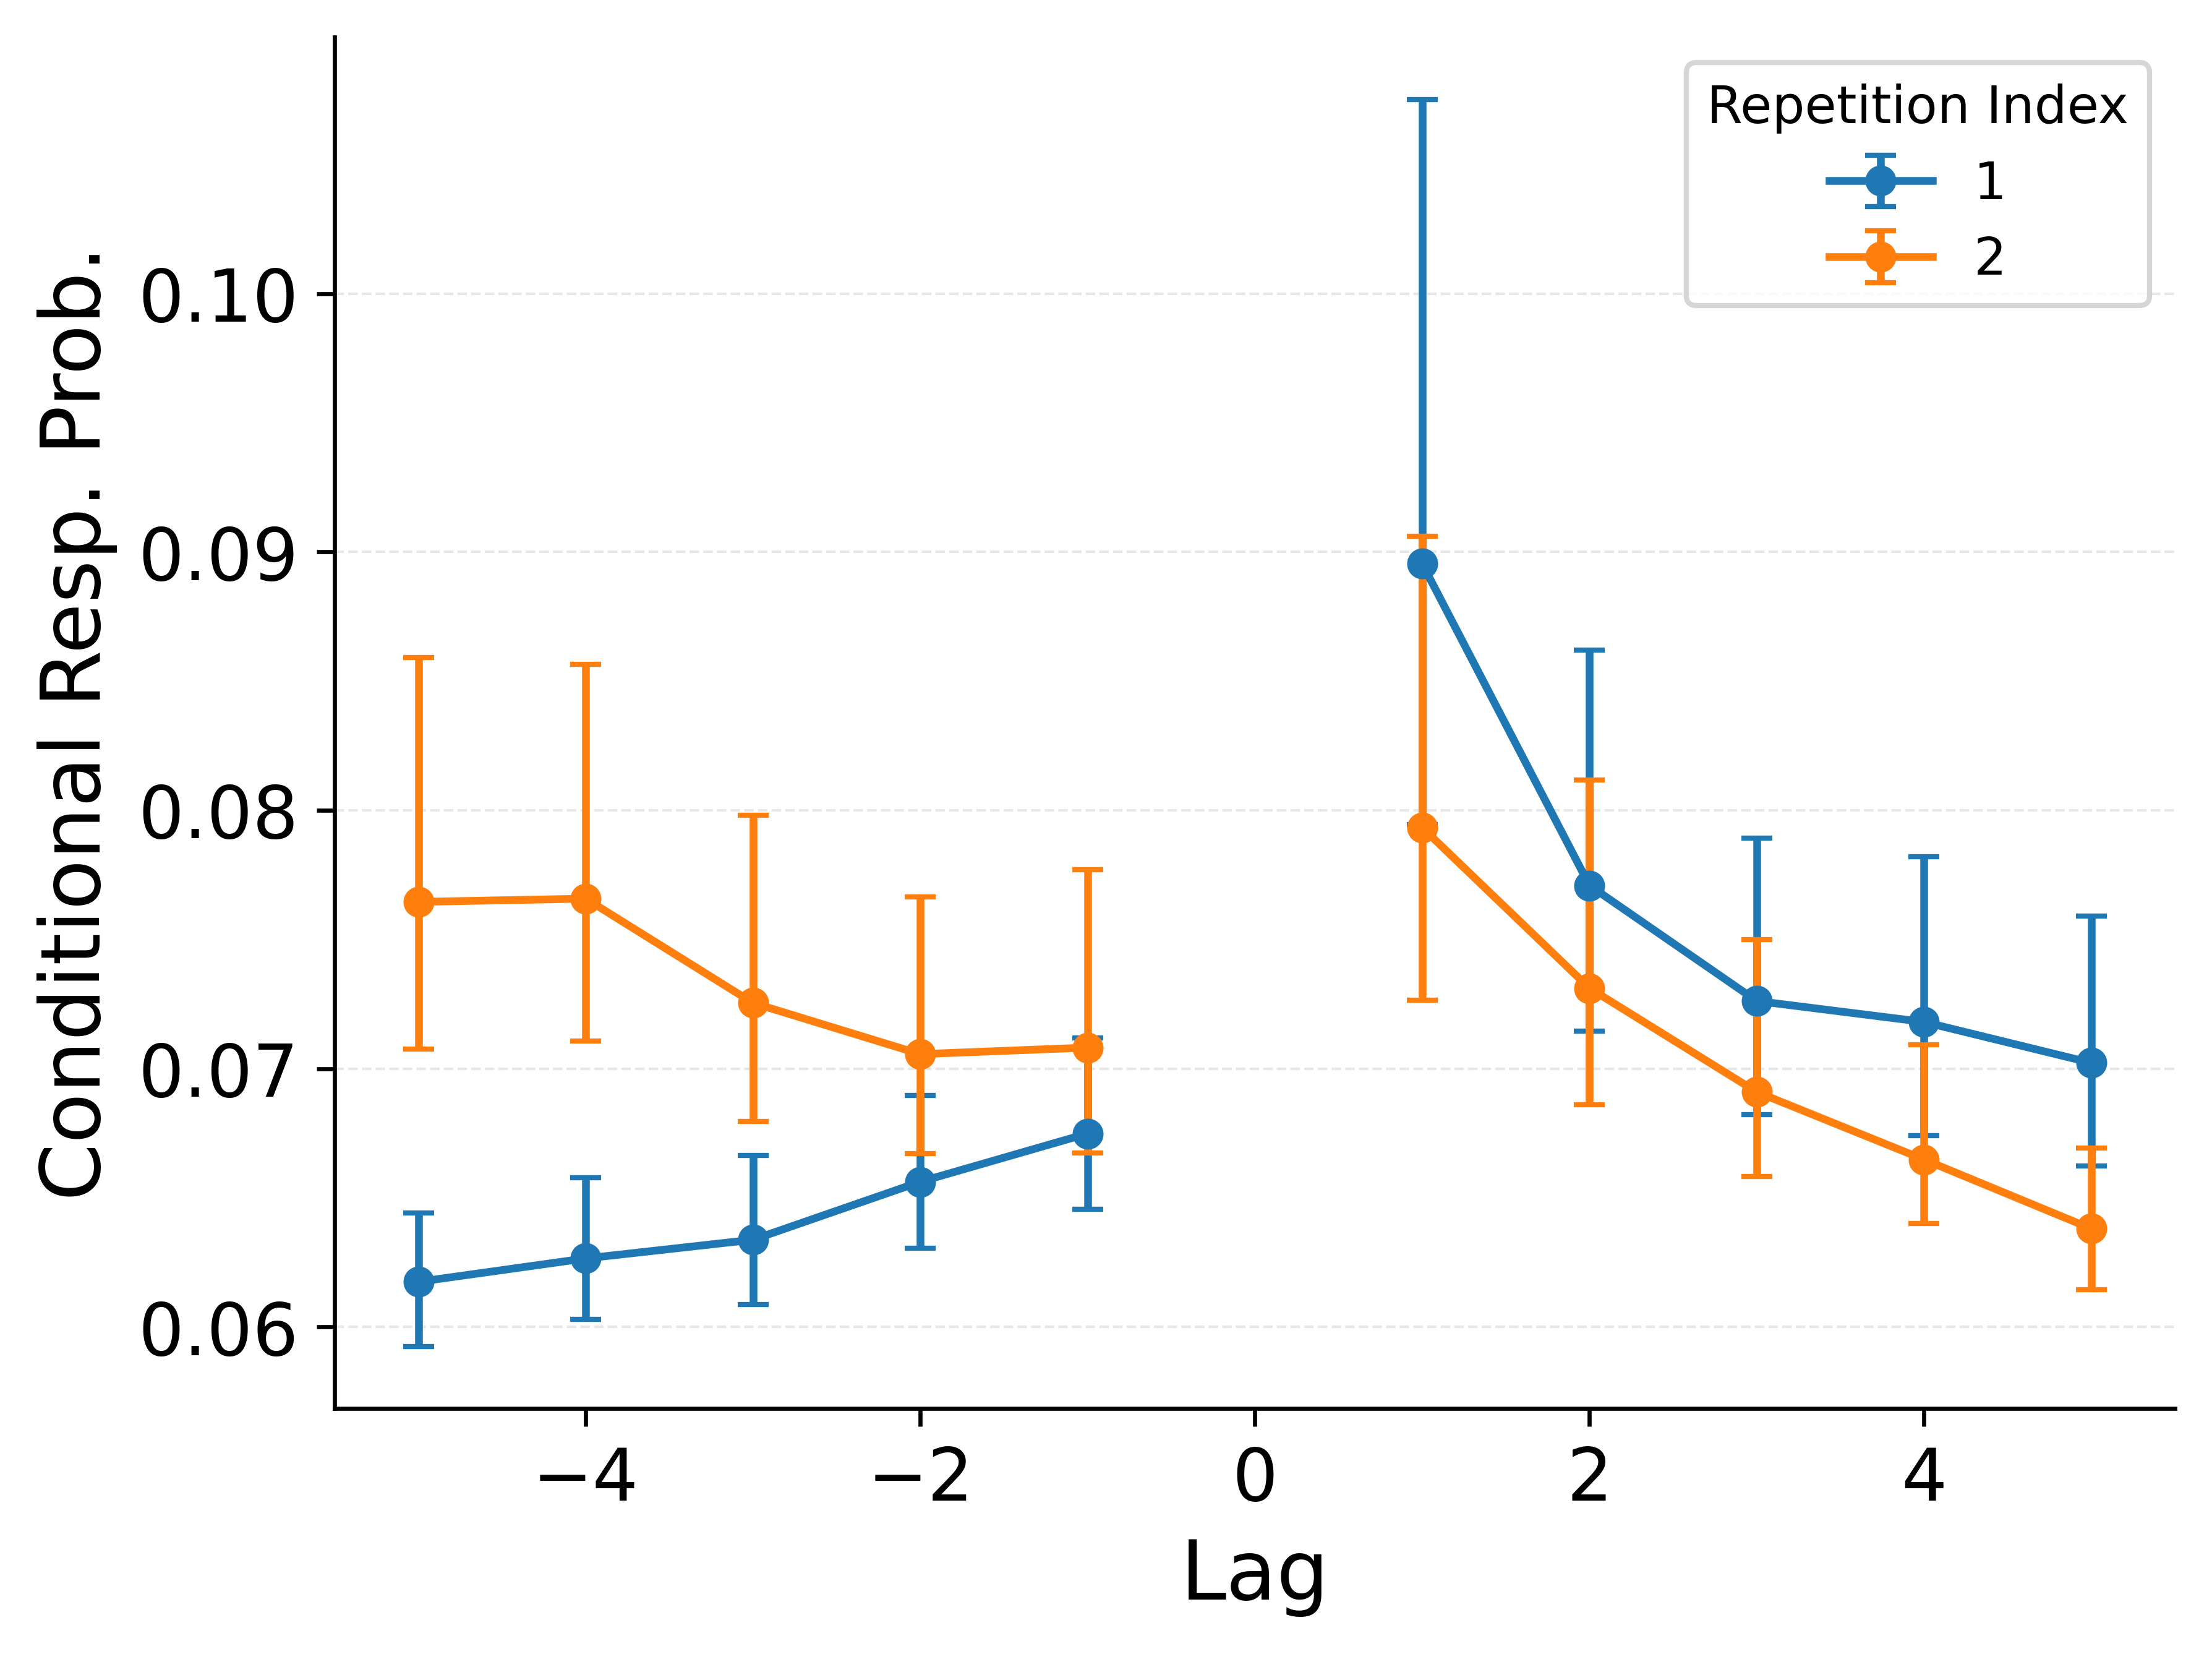
\includegraphics{../../work/thesis/figures/RepeatedRecallsLohnasKahana2014_control_WeirdCMR_full_best_of_3_LT34_rep_crp.png}\end{minipage}%

\end{figure}%

\subsection{Backward/Incoming Variant of the Repetition
Lag-CRP}\label{backwardincoming-variant-of-the-repetition-lag-crp}

For each recall of a repeater, we look one step back to the item
produced immediately before it and compute two centered lag-CRPs---one
centered on the first presentation and one on the second---using the
matched, symmetric baseline to control position effects. In the data
(Figure~\ref{fig-backward_rep_lag_crp}, top row), arrivals at repeaters
come disproportionately from the backward neighbor of the \emph{first}
presentation (from \(i{-}1\) to \(i\)) compared with the backward
neighbor of the second (from \(j{-}1\) to \(j\)). The preference is
strongest in mixed lists but is also evident in the position-matched
baseline, indicating that it reflects general serial-order dynamics
(e.g., forward contiguity and output competition) rather than
repetition-specific knitting per se.

Standard CMR yields only a weak first-over-second advantage on these
incoming transitions (Figure~\ref{fig-backward_rep_lag_crp}, bottom
row), consistent with the model's tendency to aggregate support across a
repeater's occurrences and thereby dilute approach biases. Practically,
this pattern cautions that any first-over-second asymmetry seen
\emph{after} recalling a repeater (the outgoing analysis) may be partly
inherited from how the search state approached the repeater; the
mixed--minus--baseline contrast in the outgoing test is therefore the
cleaner probe of repetition-specific reinstatement.

\begin{figure}

\caption{\label{fig-backward_rep_lag_crp}Repetition lag-CRP
(incoming/backward): data vs CMR. Top row (data): mixed lists (left) and
baseline (right) for transitions to repeated items. Bottom row (CMR):
simulations. In data, transitions to repeated items are more frequently
from the backward neighbor of the item's first presentation than from
the second, especially in mixed lists but also in the position-matched
baseline. By contrast, CMR predicts a weaker first-over-second advantage
for incoming transitions.}

\begin{minipage}{0.50\linewidth}
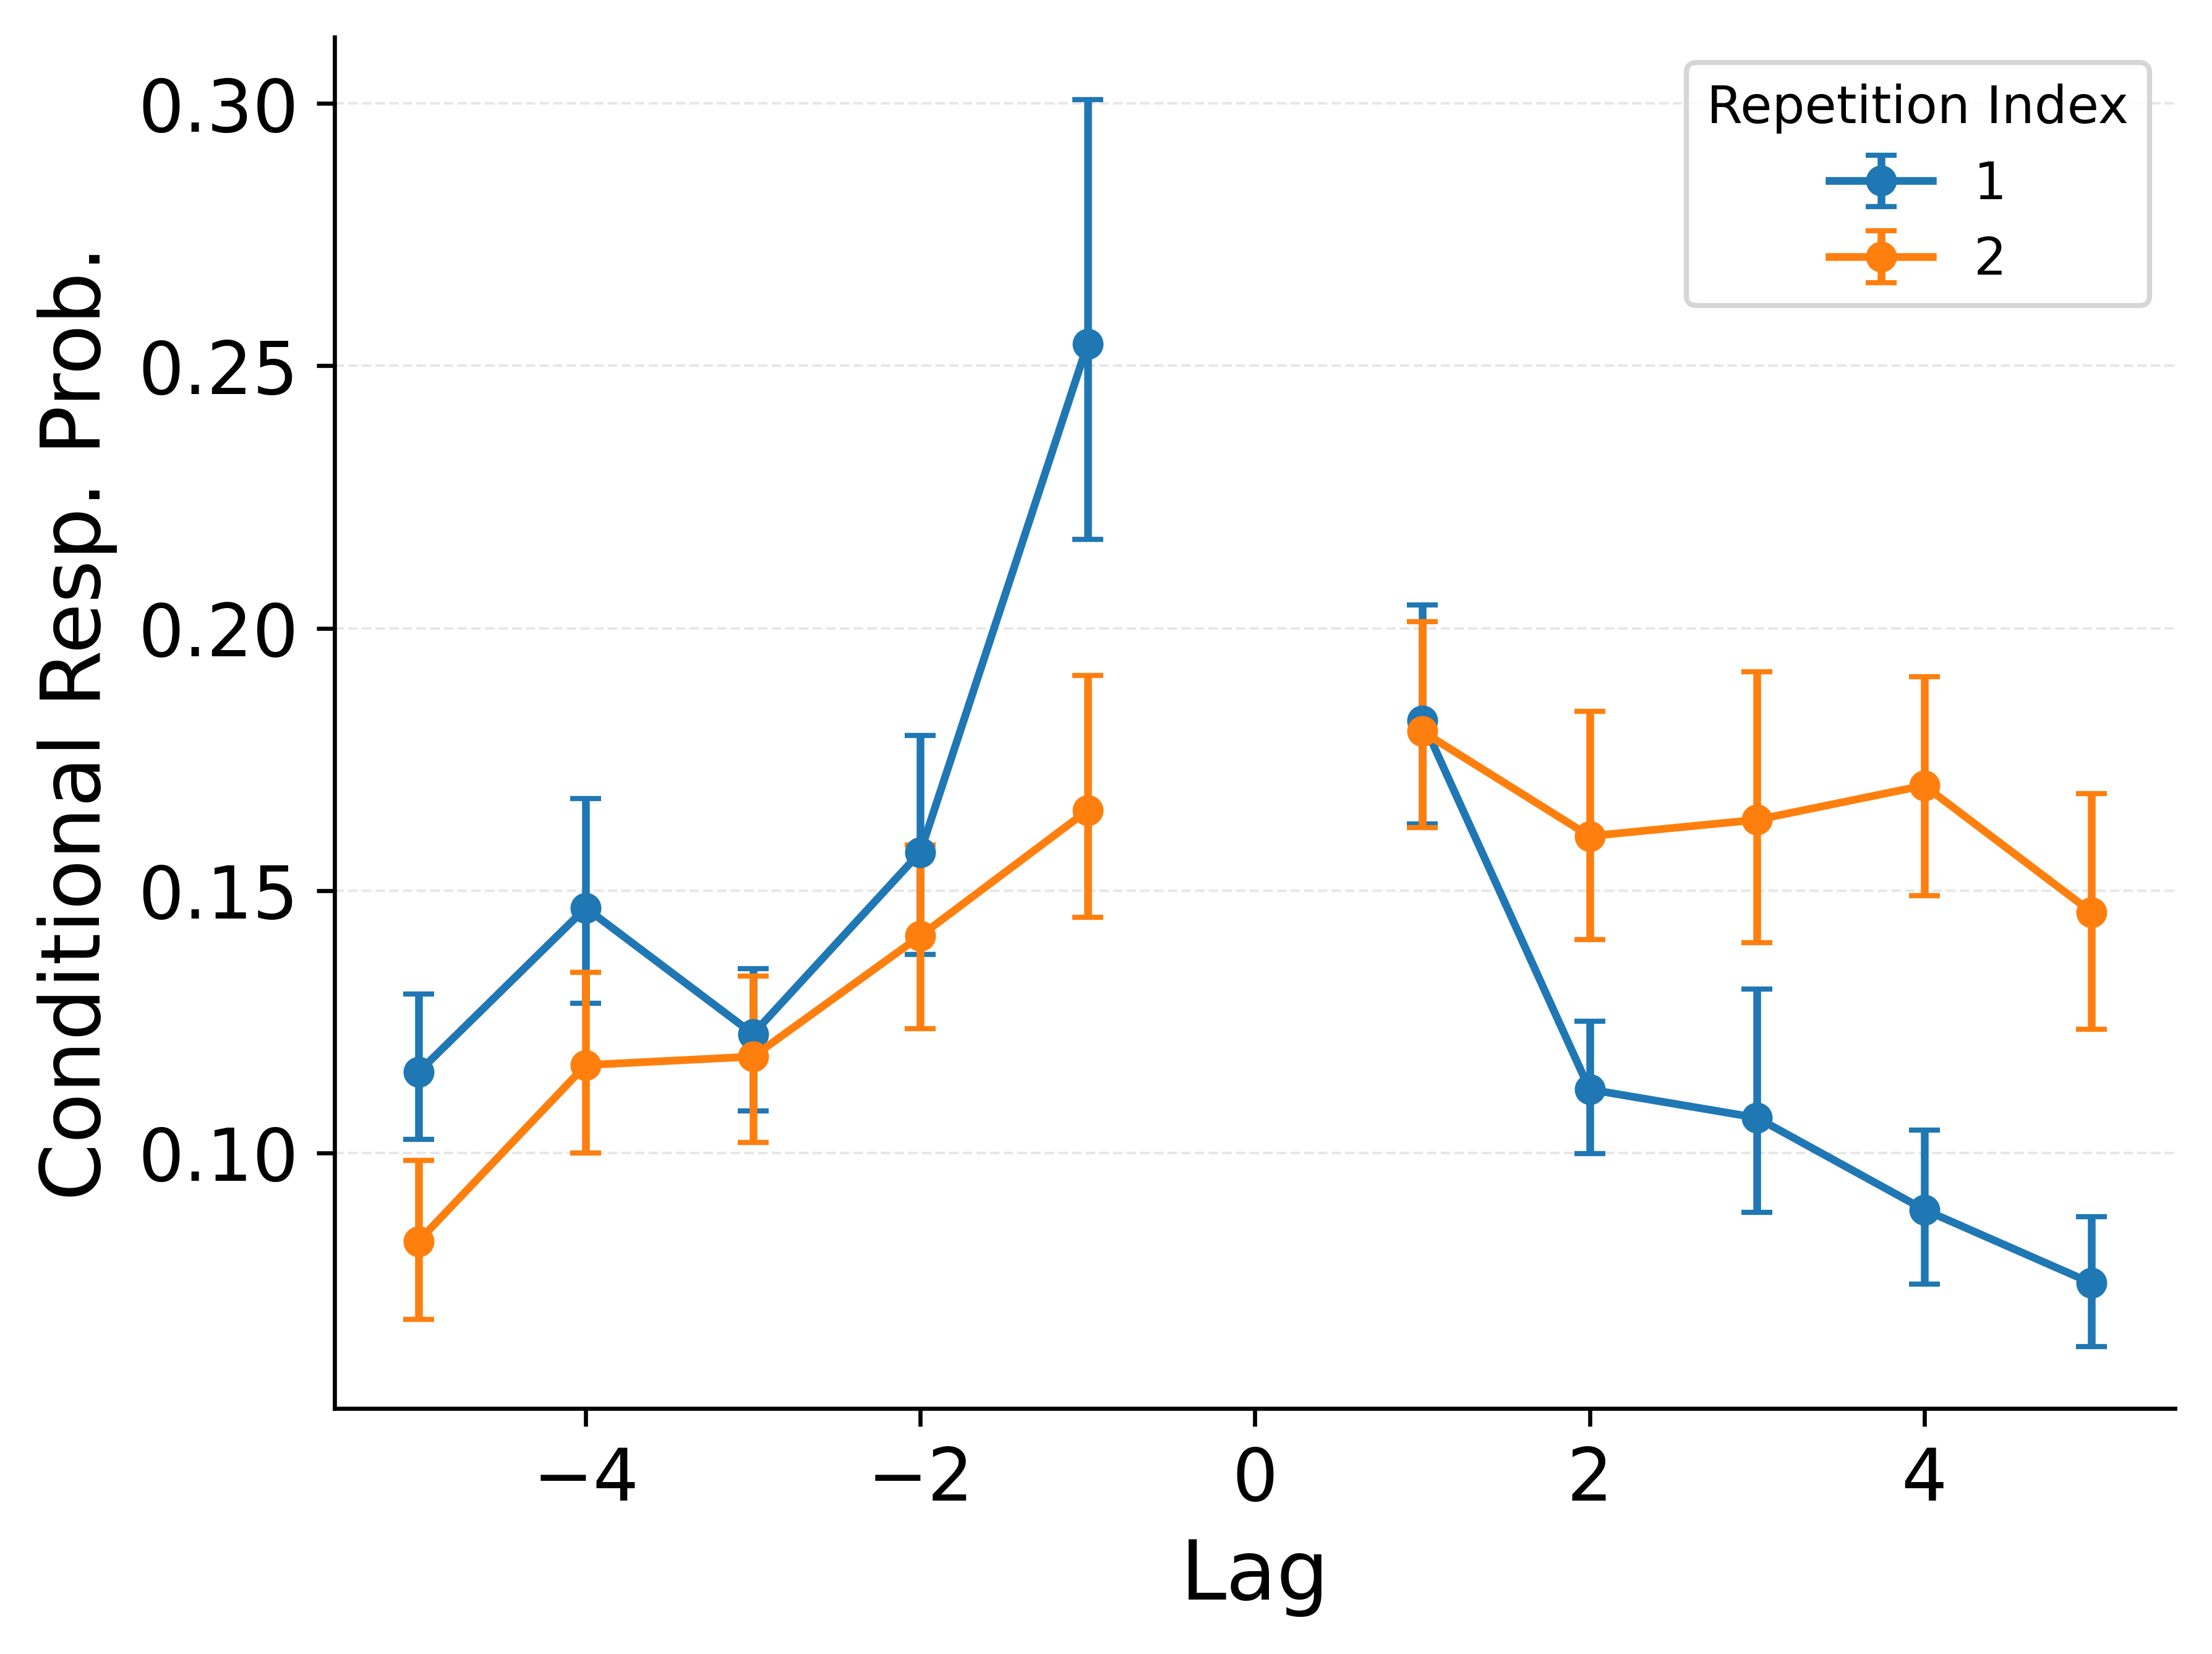
\includegraphics{../../work/thesis/figures/RepeatedRecallsLohnasKahana2014_mixed_data_full_best_of_3_LT34_back_rep_crp.png}\end{minipage}%
%
\begin{minipage}{0.50\linewidth}
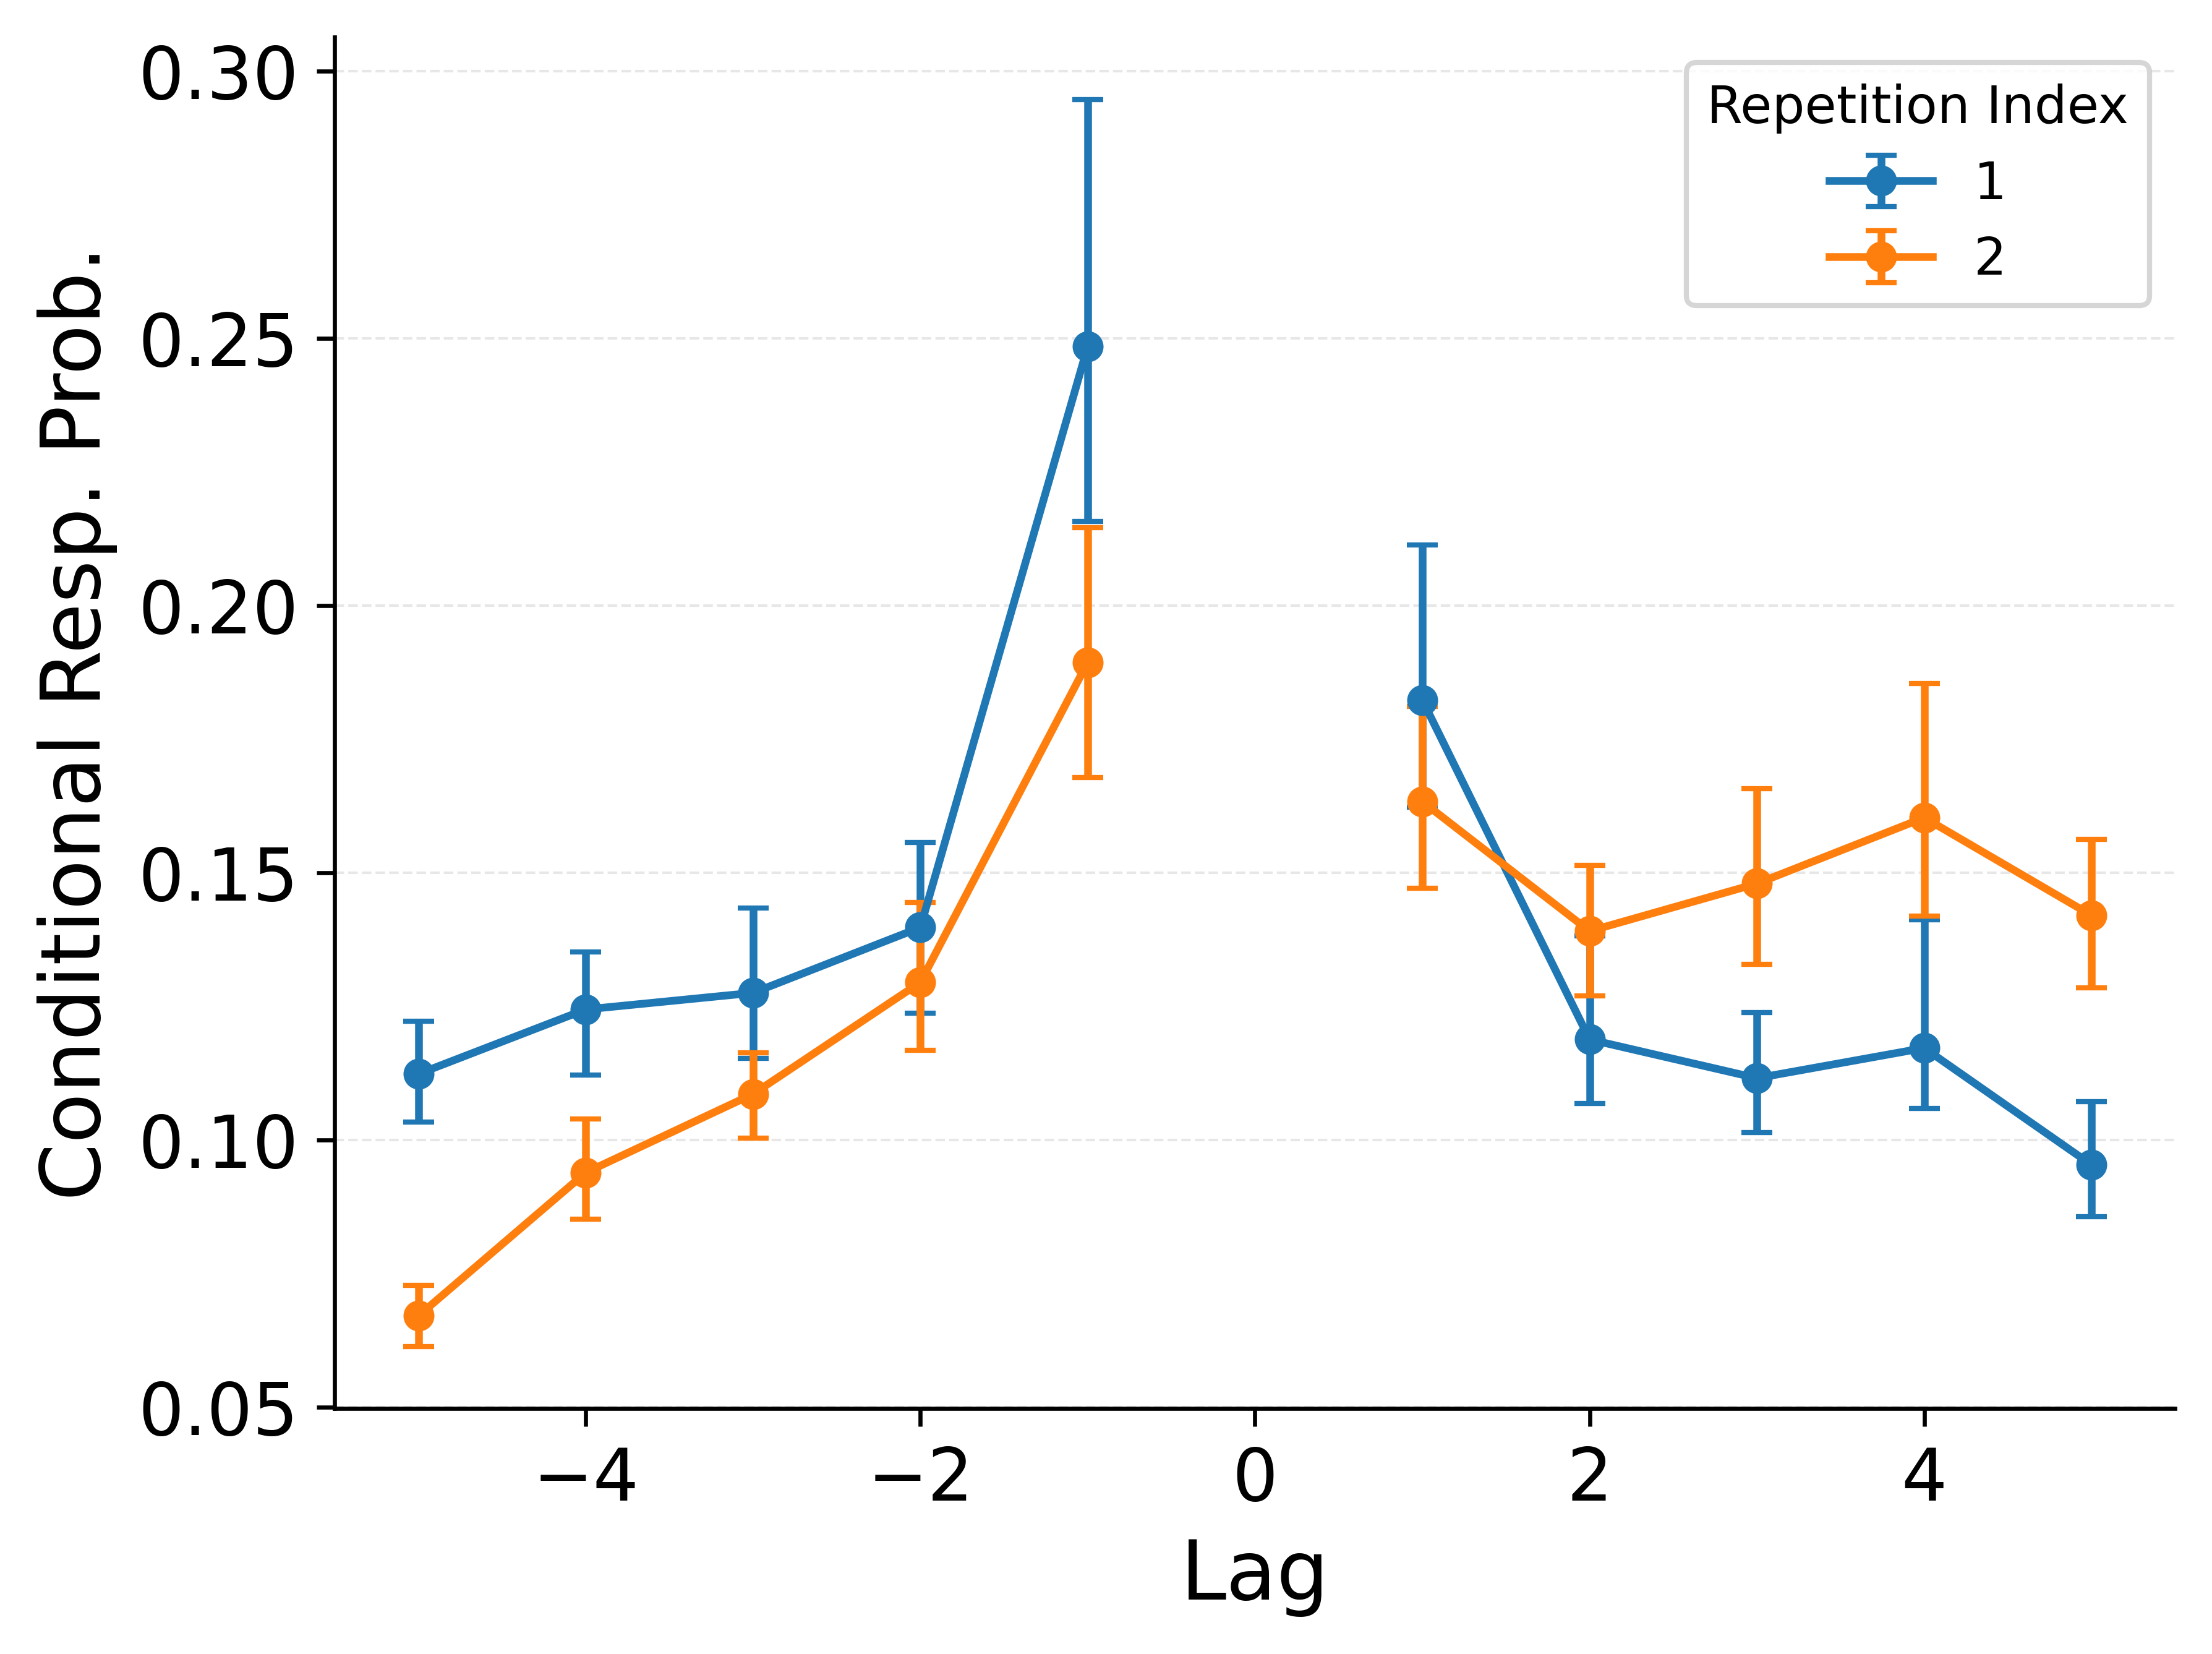
\includegraphics{../../work/thesis/figures/RepeatedRecallsLohnasKahana2014_control_data_full_best_of_3_LT34_back_rep_crp.png}\end{minipage}%
\newline
\begin{minipage}{0.50\linewidth}
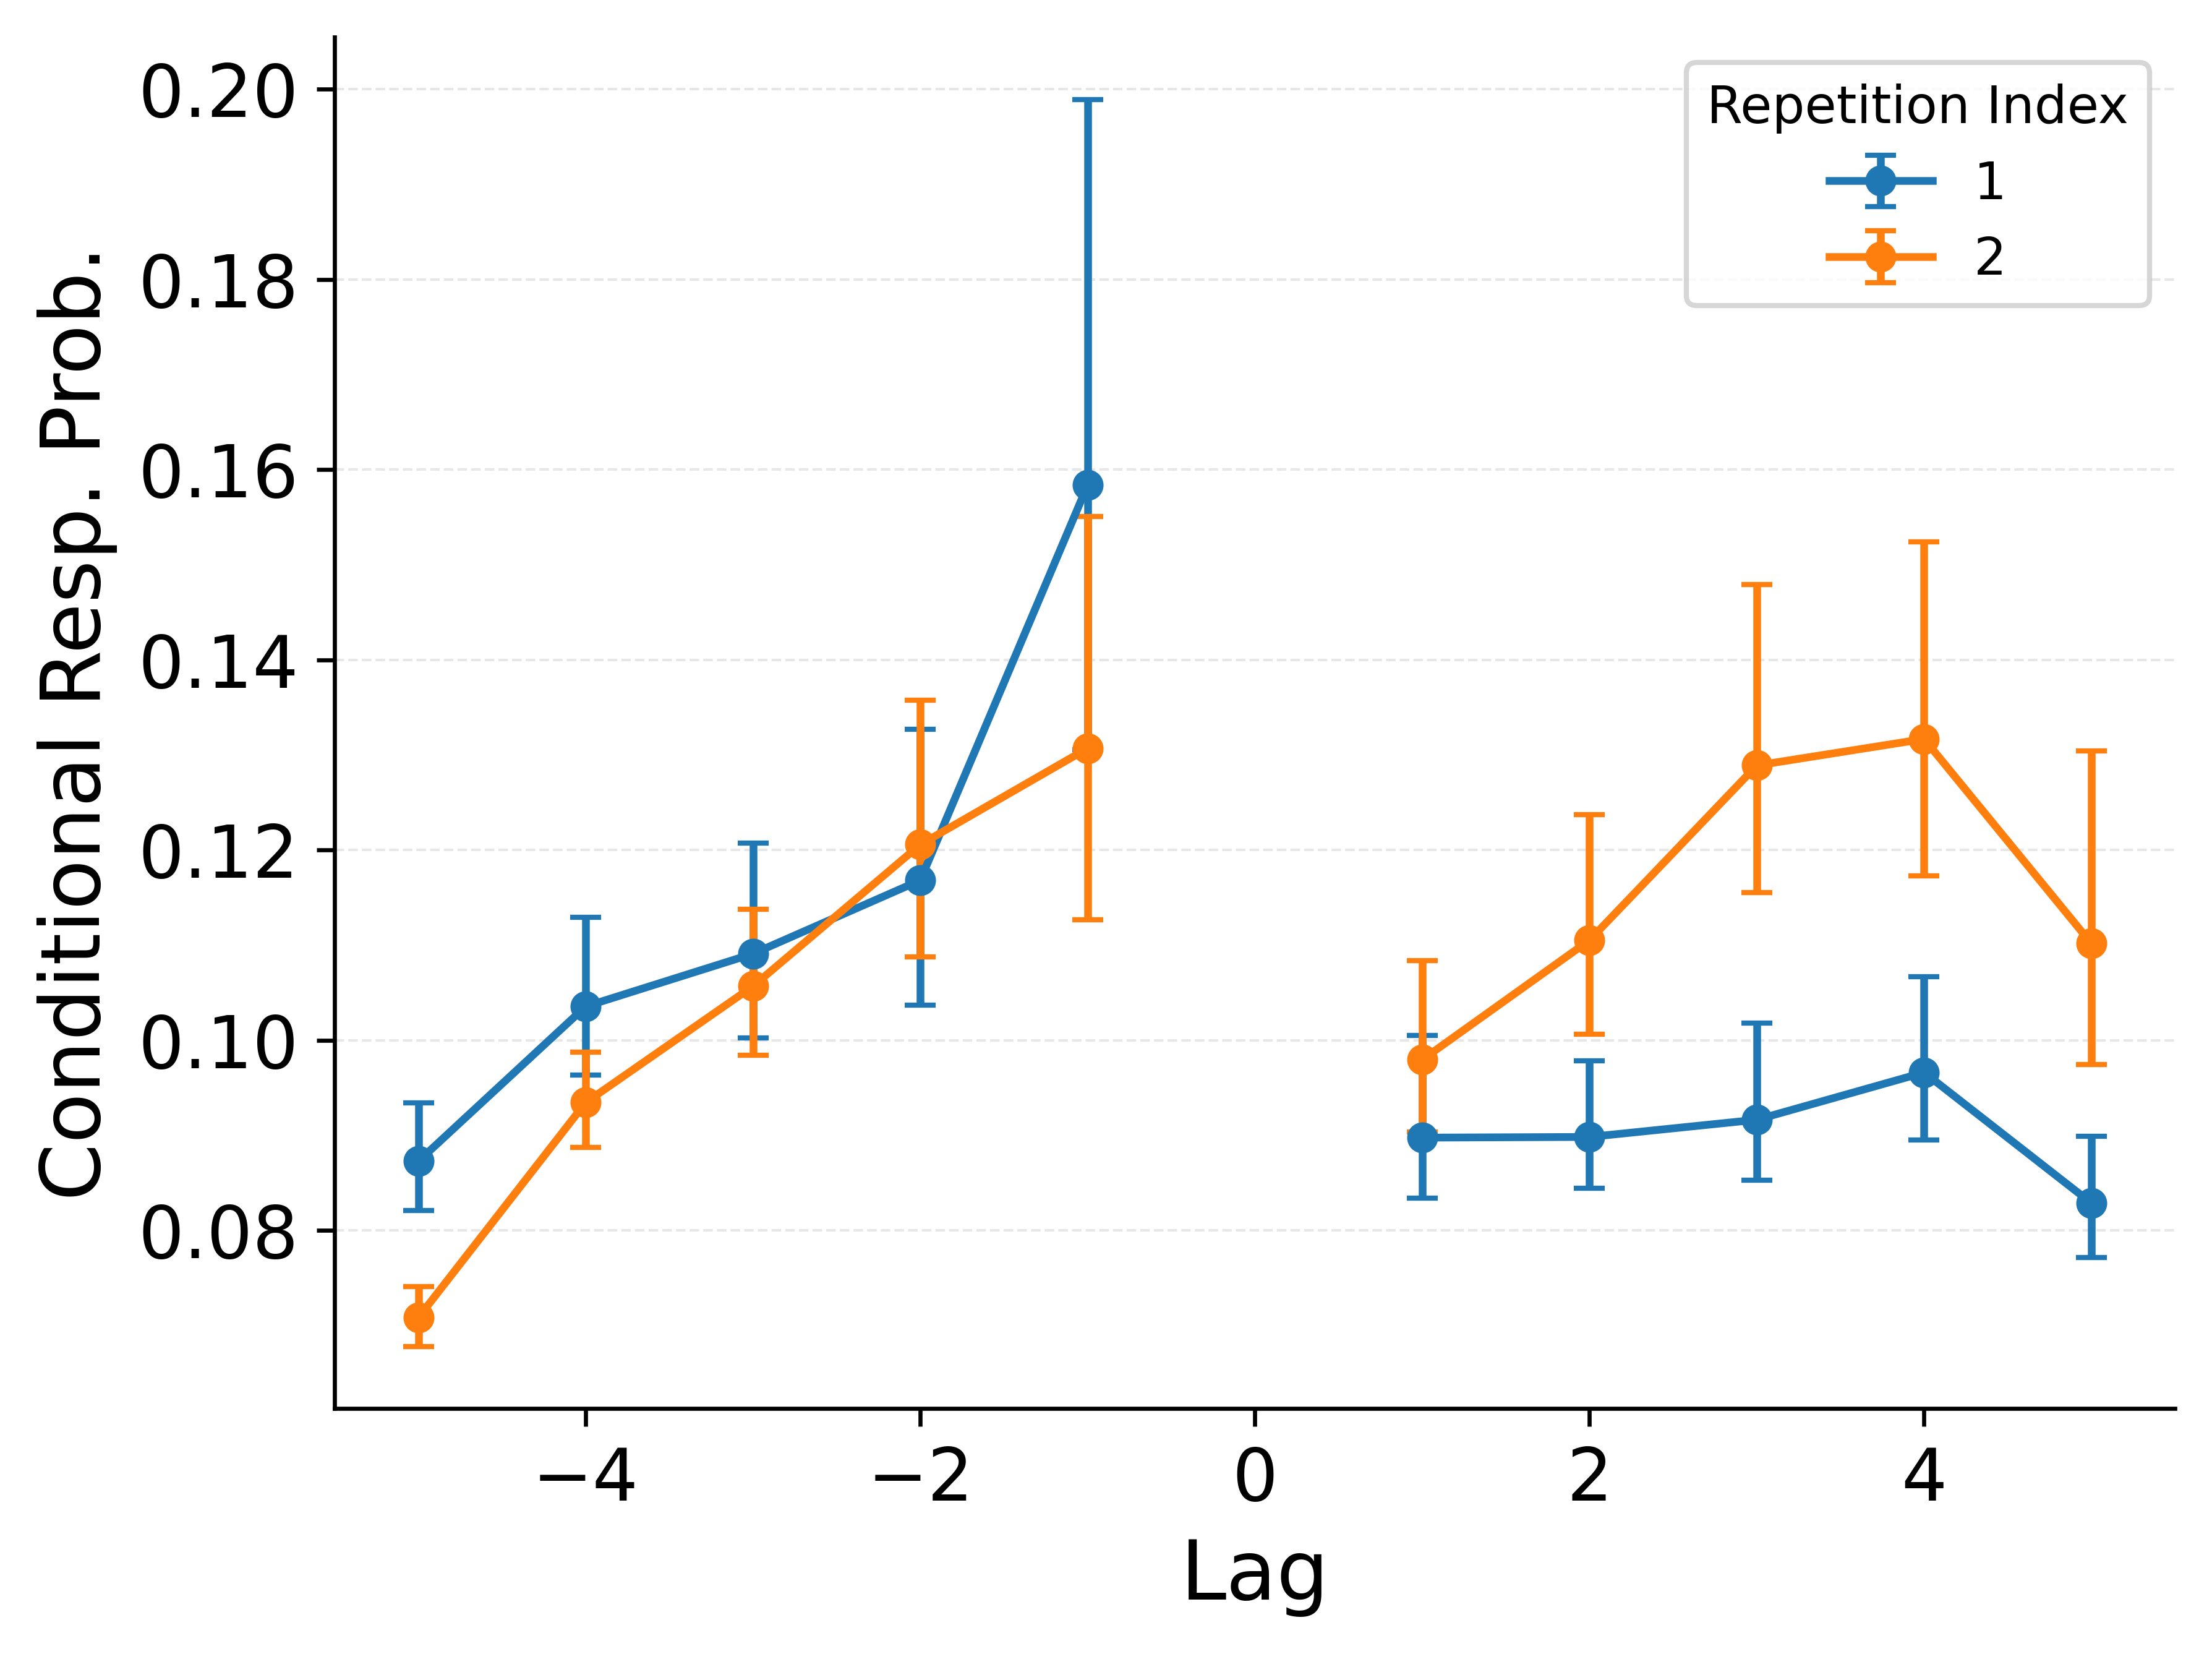
\includegraphics{../../work/thesis/figures/RepeatedRecallsLohnasKahana2014_mixed_WeirdCMR_full_best_of_3_LT34_back_rep_crp.png}\end{minipage}%
%
\begin{minipage}{0.50\linewidth}
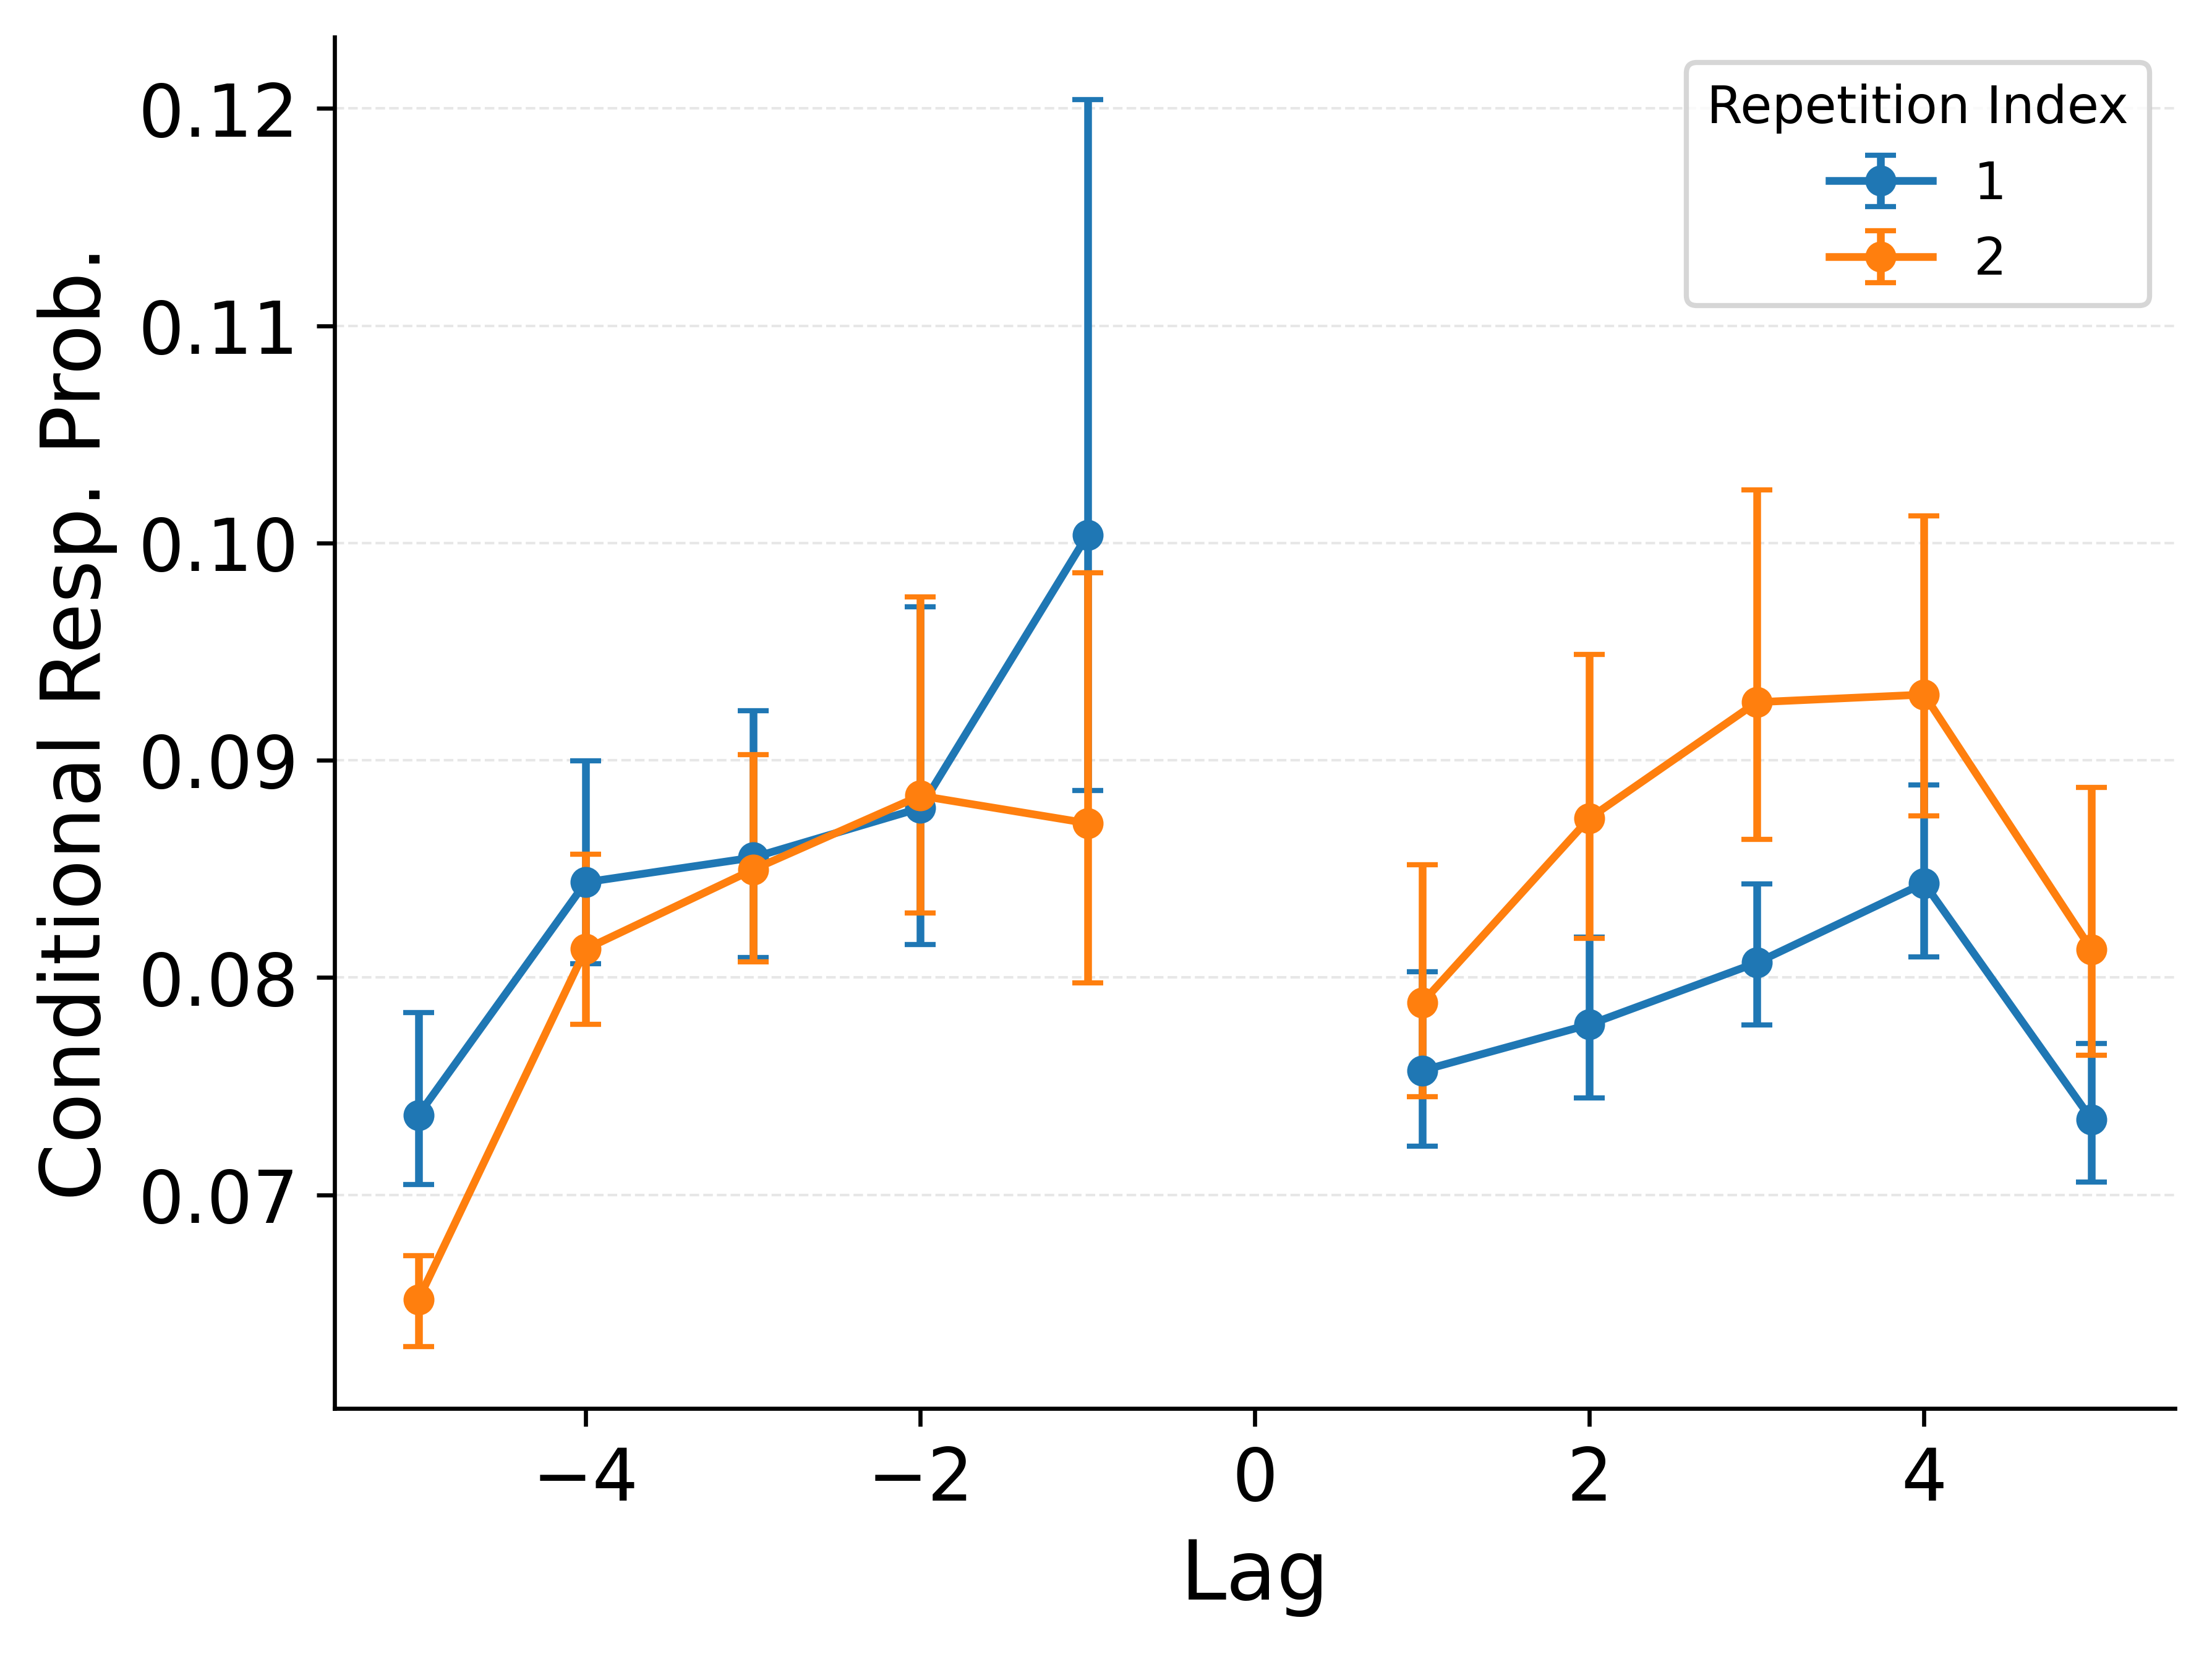
\includegraphics{../../work/thesis/figures/RepeatedRecallsLohnasKahana2014_control_WeirdCMR_full_best_of_3_LT34_back_rep_crp.png}\end{minipage}%

\end{figure}%

\subsection{Forward Chaining in Serial
Recall}\label{forward-chaining-in-serial-recall}

Serial recall provides a more stringent test of cross-occurrence
competition. In the data from Logan
(\citeproc{ref-logan2021serial}{2021}) and from Kahana and Jacobs
(\citeproc{ref-kahana2000interresponse}{2000})
(Figure~\ref{fig-serial_rep_crp}, top), after participants correctly
type through the first occurrence at position \(i\), continuations to
\(i{+}1\) remain strong, and erroneous continuations to the competing
neighbor \(j{+}1\) are rare and indistinguishable from the matched
control baseline. That is, the second occurrence's neighborhood does not
draw responses away from the correct forward chain.

In the bottom half of Figure~\ref{fig-serial_rep_crp}, simulations of
standard CMR after fitting to each dataset predicts a measurable
elevation of \(i\!\rightarrow\!j{+}1\) errors relative to baseline,
again reflecting blended support across occurrences. The absence of this
cross-occurrence forward error in the data generalizes the
non-interference finding from free recall to a serial-order task:
whether the next step is unconstrained (free recall) or constrained
(serial recall), occurrences behave as if support is routed through a
single episode.

\begin{figure}

\caption{\label{fig-serial_rep_crp}\textbf{Cross-occurrence forward
errors in serial recall (two datasets).} Left: Logan
(\citeproc{ref-logan2021serial}{2021}). Right: Kahana and Jacobs
(\citeproc{ref-kahana2000interresponse}{2000}). \textbf{Top row (data):}
For items studied at positions \(i\) and \(j\), each panel plots the
conditional probability--- after correct report through the first
occurrence at position \(i\) -- of an erroneous transition to the
\emph{second} occurrence's forward neighbors (\(i\!\rightarrow\!j{+}1\)
and \(i\!\rightarrow\!j{+}2\)), contrasting mixed lists with their
position-matched, symmetric baseline. \textbf{Bottom row (CMR):}
standard CMR simulations fitted separately to each dataset and scored
with the identical baseline procedure. In both datasets, data show no
elevation of \(i\!\rightarrow\!j{+}1/j{+}2\) errors relative to baseline
(non-interference), whereas CMR predicts a clear error elevation
(associative interference).}

\begin{minipage}{0.50\linewidth}
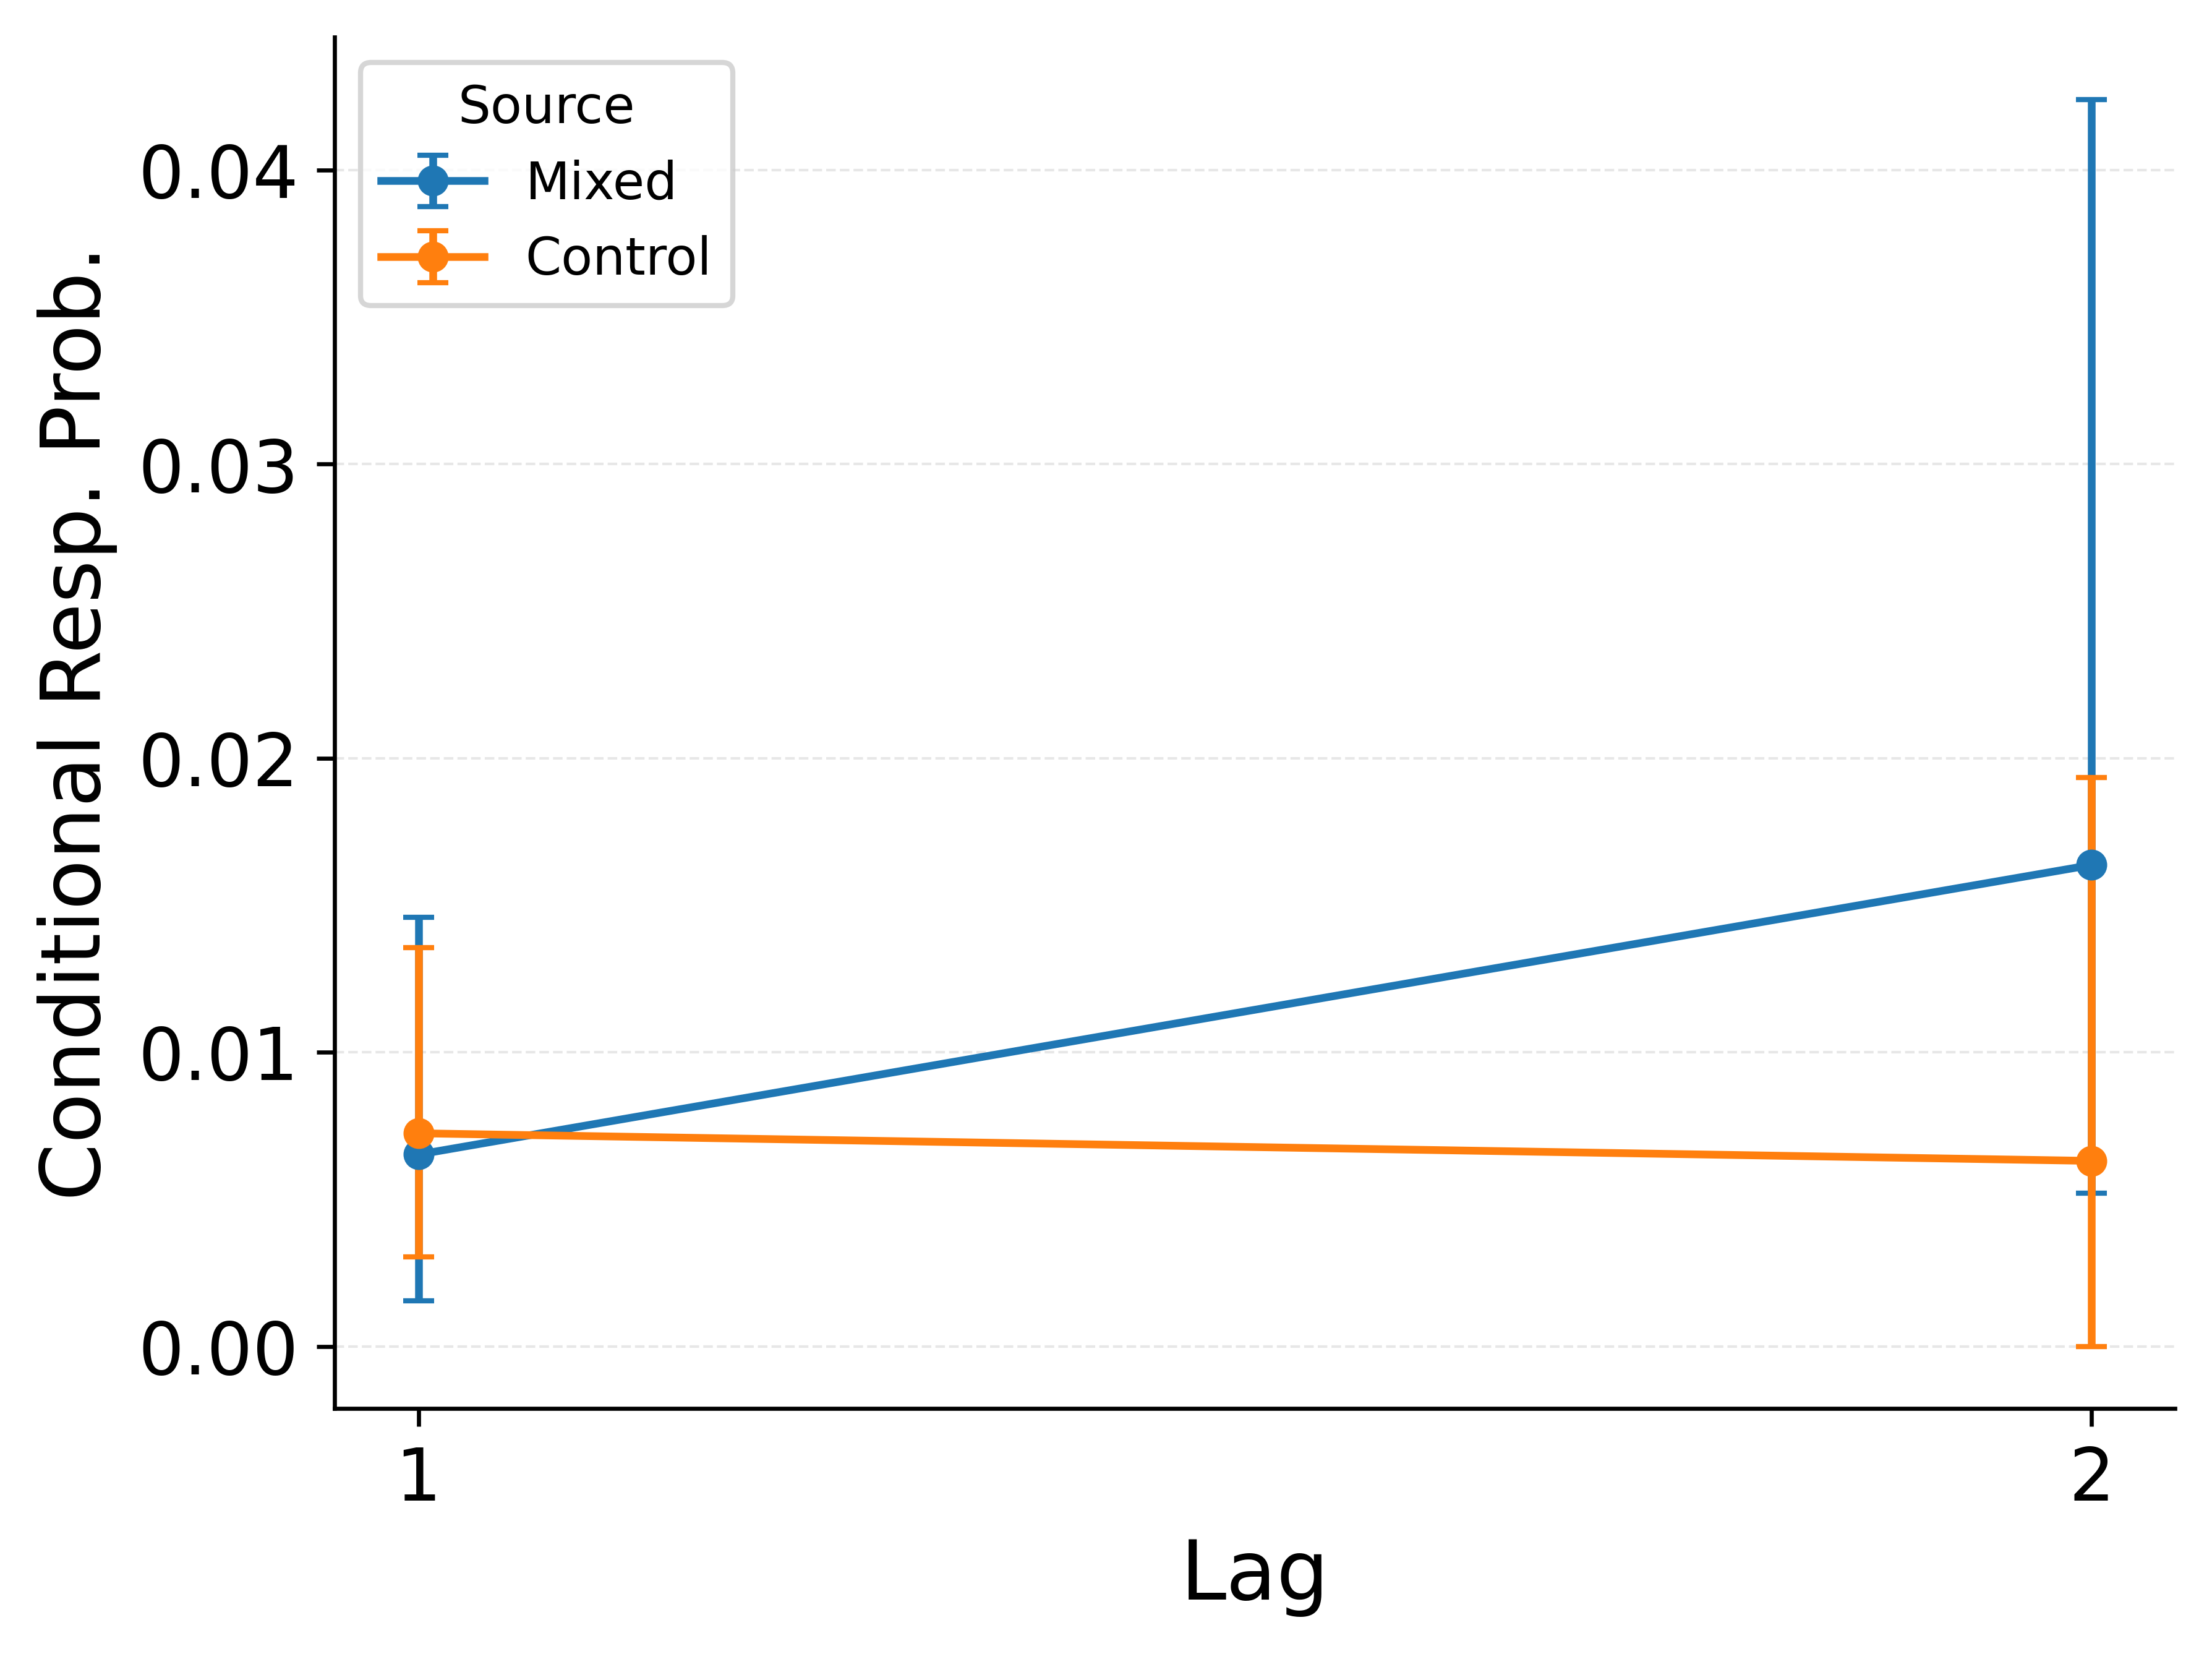
\includegraphics{../../work/thesis/figures/RepeatedRecallsGordonRanschburg2021_mixedvscontrolA_data_full_best_of_3_second_rep_crp.png}\end{minipage}%
%
\begin{minipage}{0.50\linewidth}
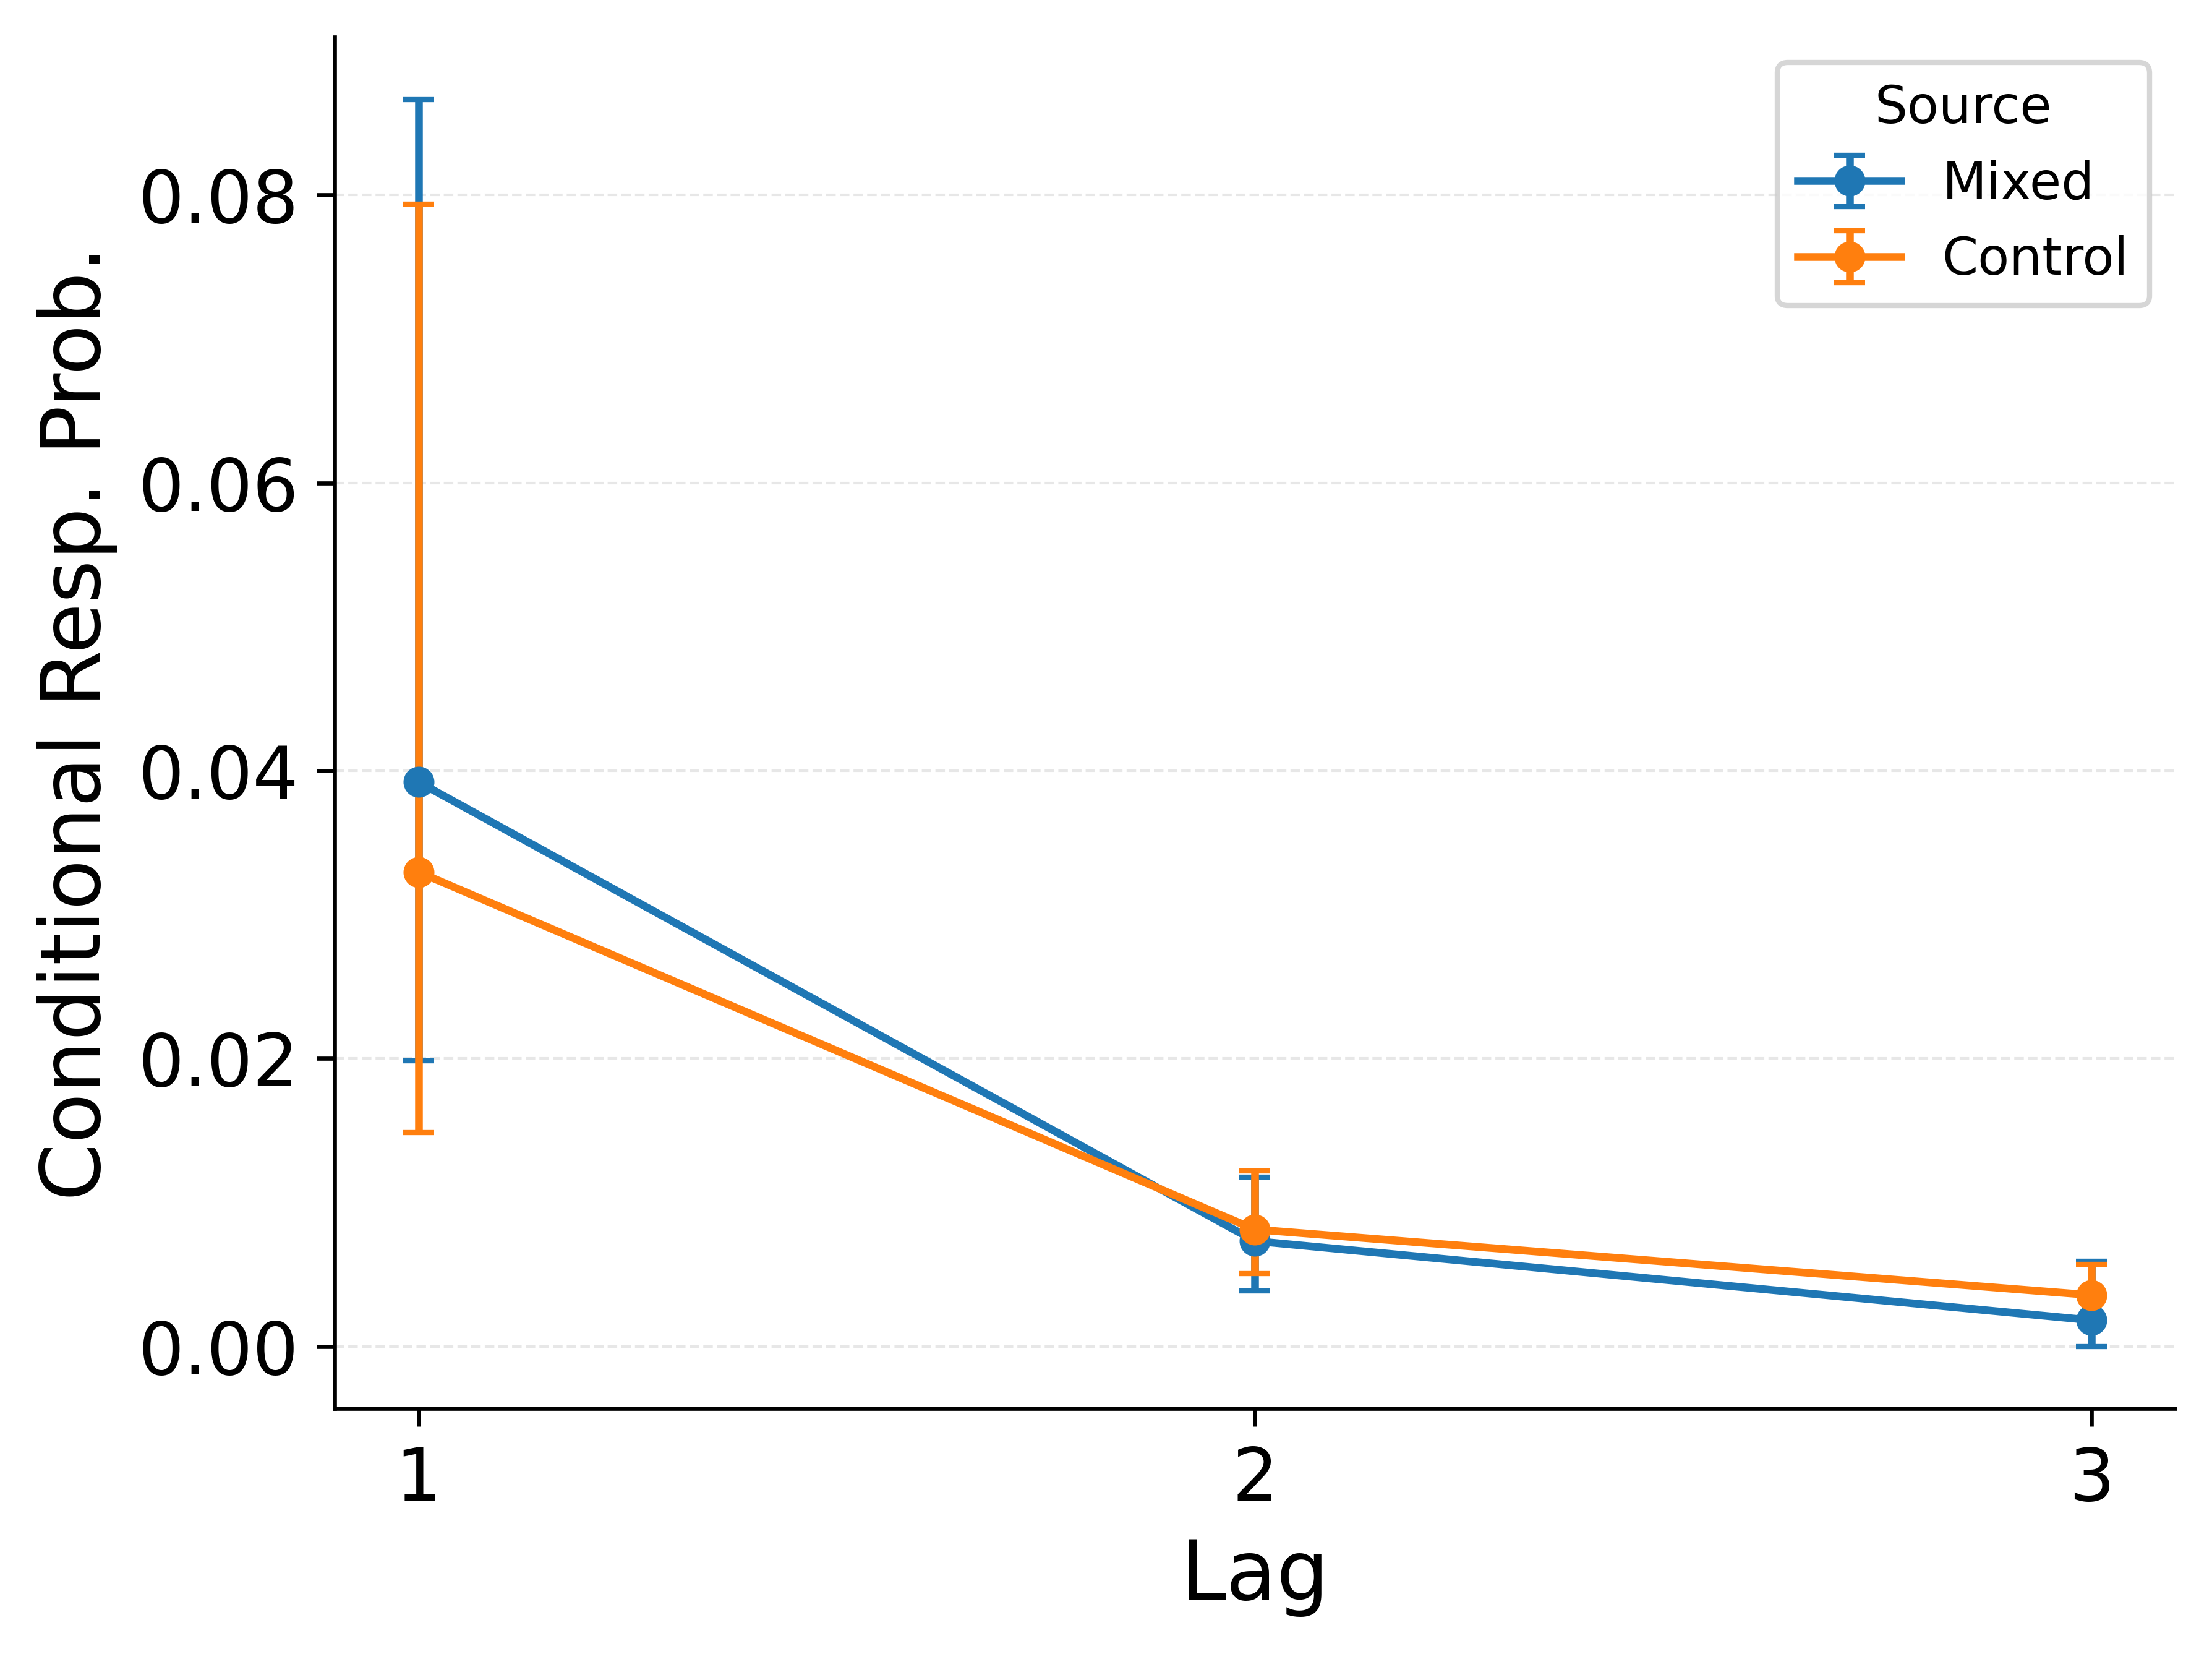
\includegraphics{../../work/thesis/figures/RepeatedRecallsKahanaJacobs2000_mixedvscontrolA_data_full_best_of_3_second_rep_crp.png}\end{minipage}%
\newline
\begin{minipage}{0.50\linewidth}
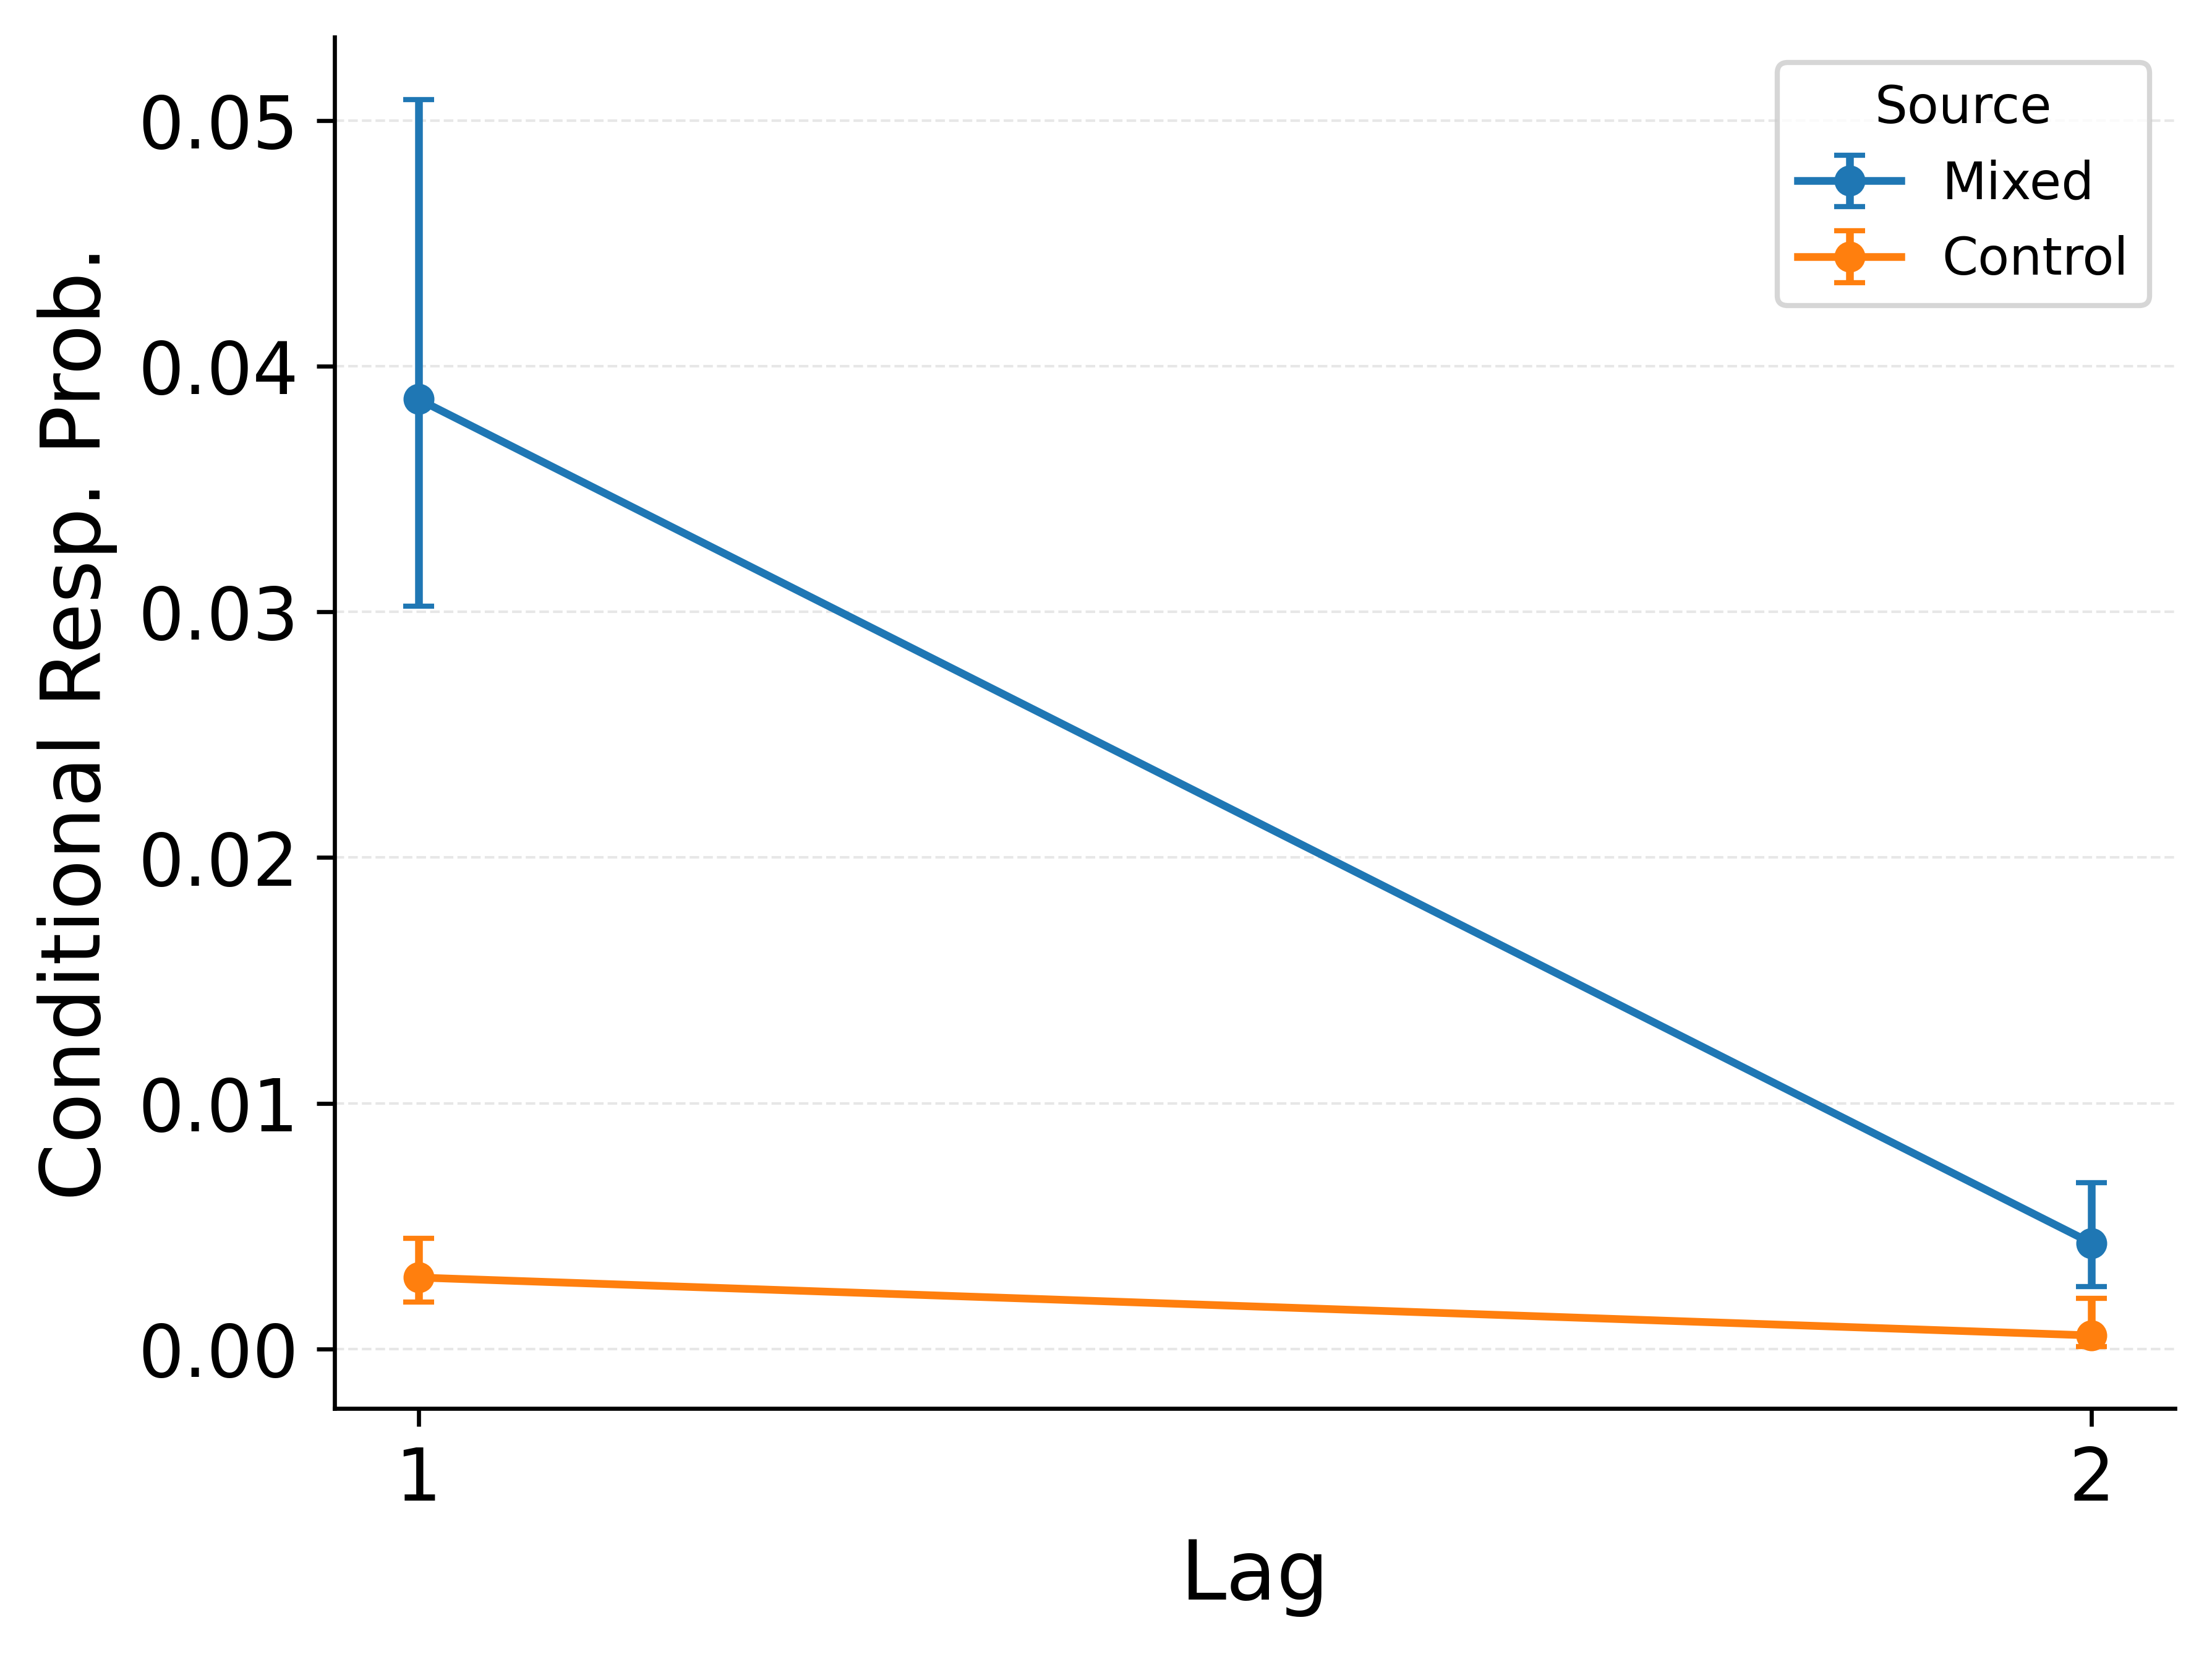
\includegraphics{../../work/thesis/figures/RepeatedRecallsGordonRanschburg2021_mixedvscontrolA_WeirdCMR_full_best_of_3_second_rep_crp.png}\end{minipage}%
%
\begin{minipage}{0.50\linewidth}
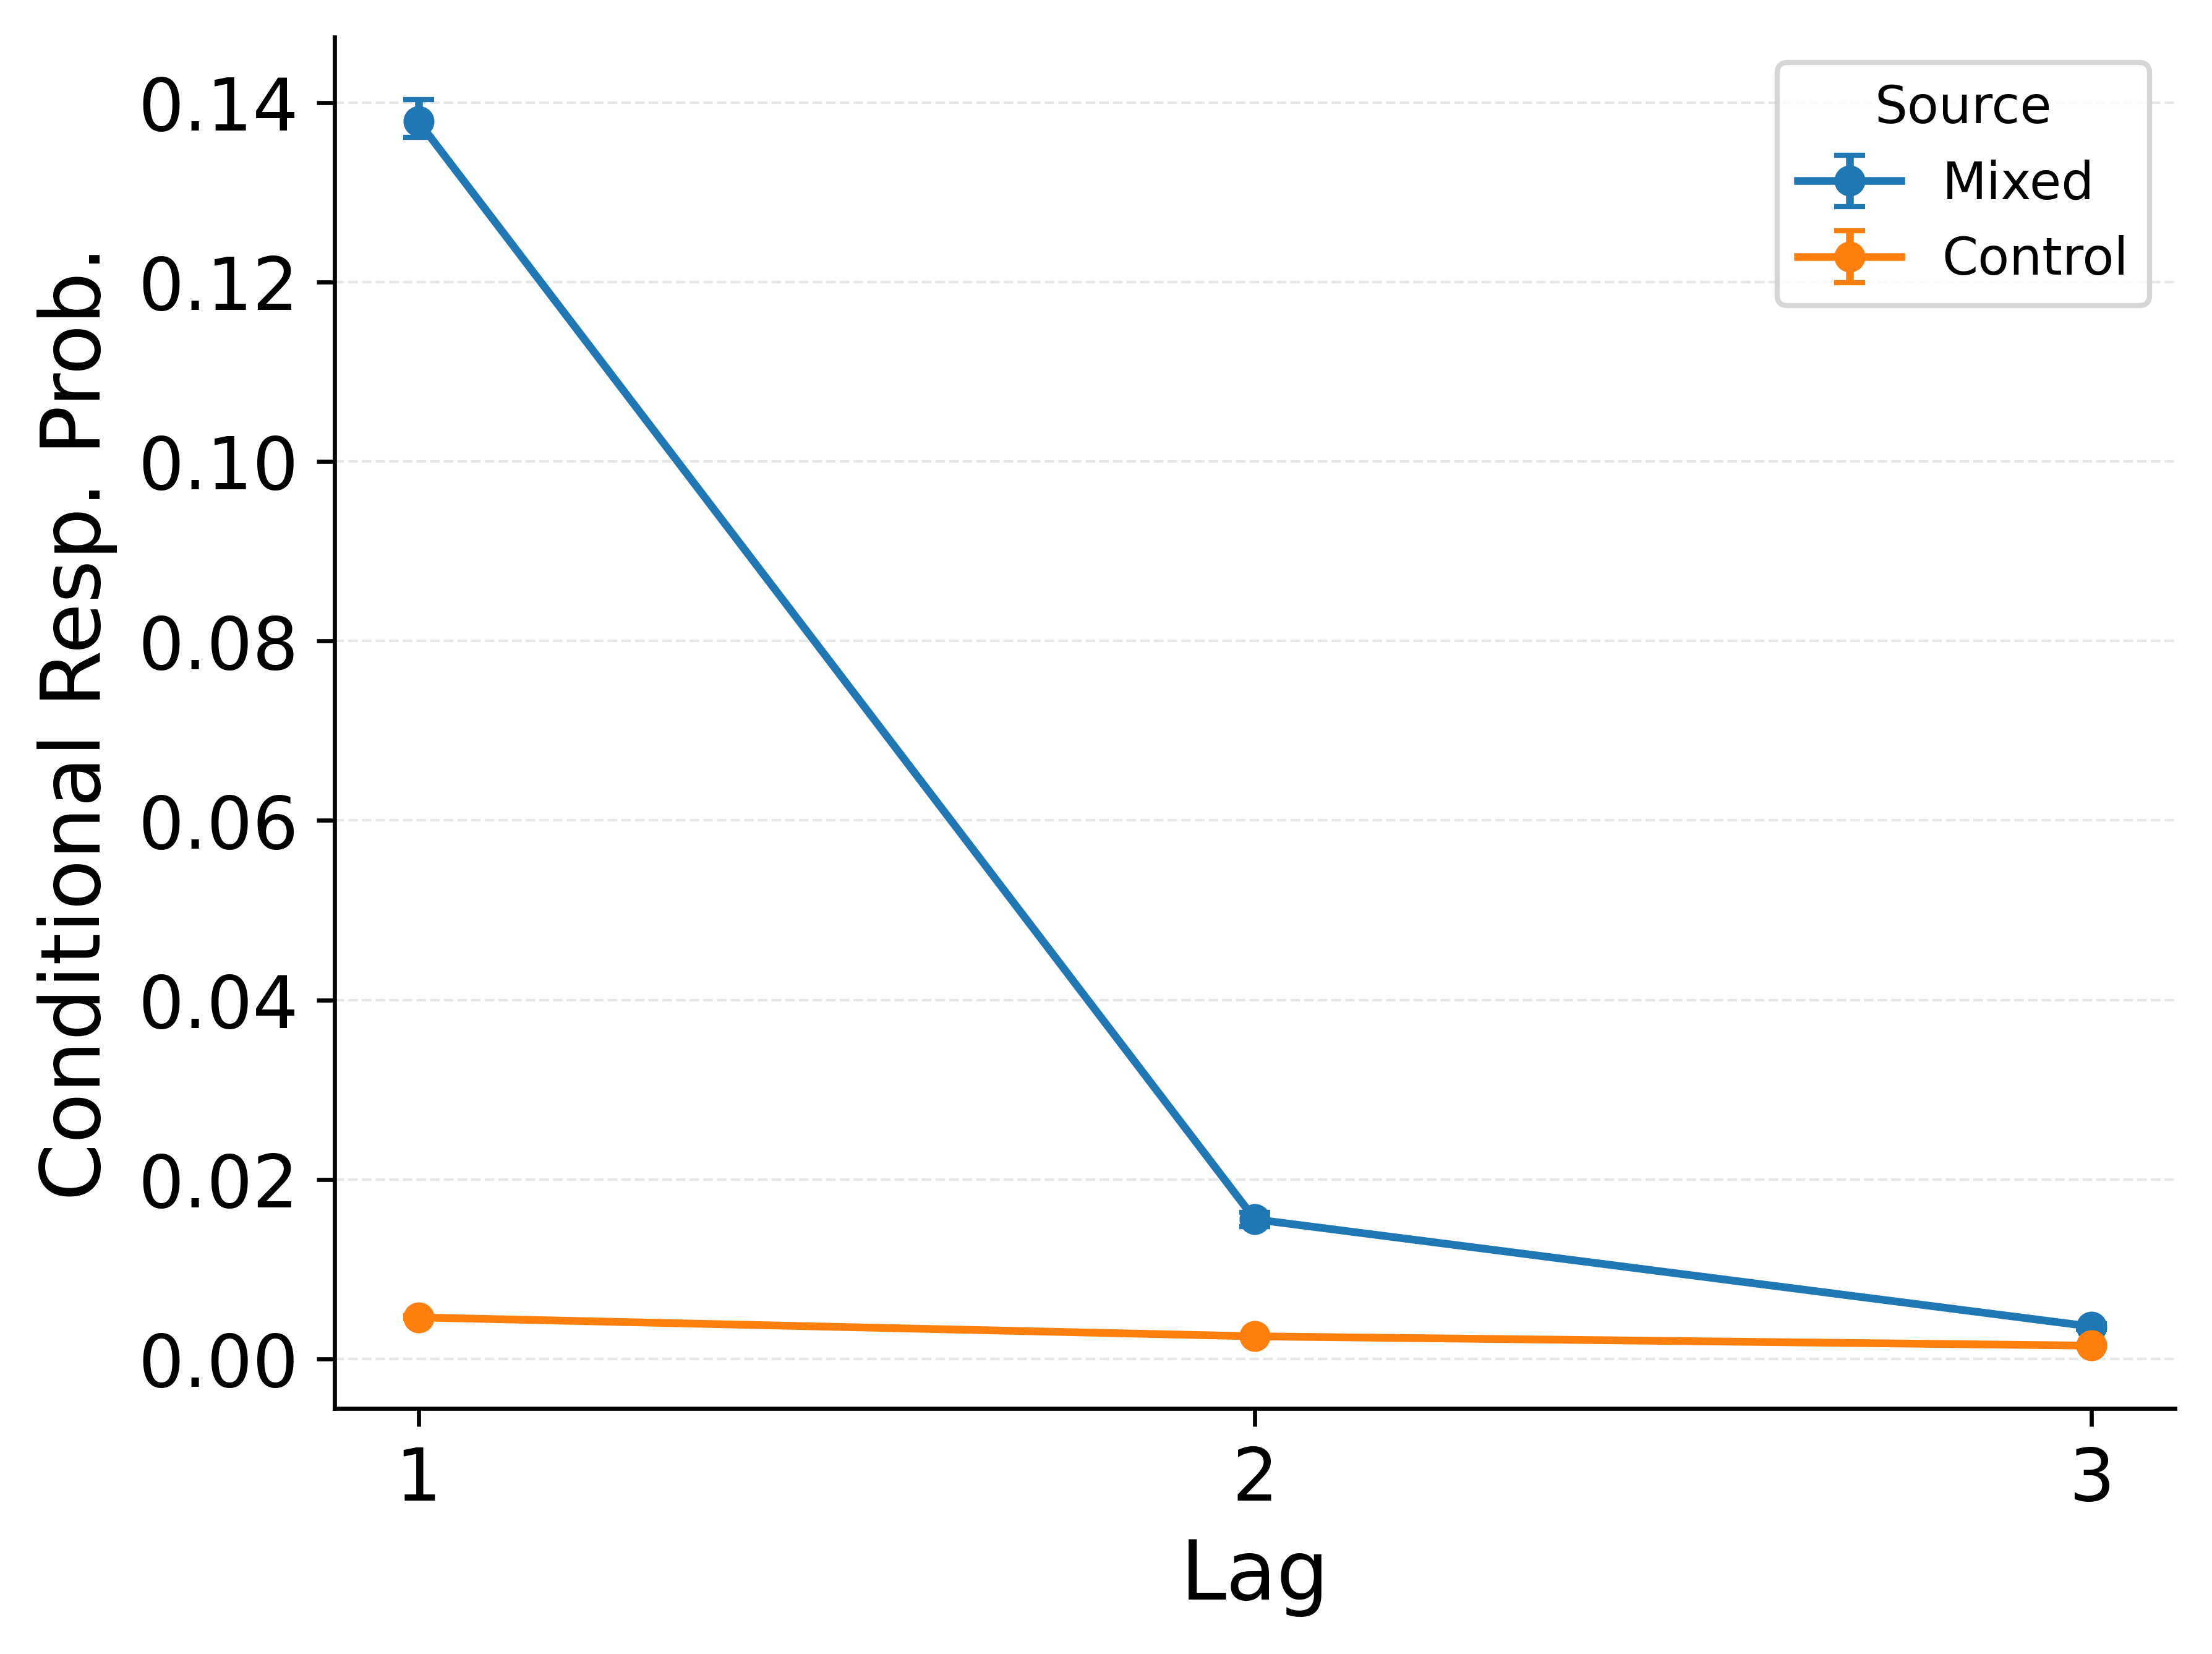
\includegraphics{../../work/thesis/figures/RepeatedRecallsKahanaJacobs2000_mixedvscontrolA_WeirdCMR_full_best_of_3_second_rep_crp.png}\end{minipage}%

\end{figure}%

\subsection{Summary: Noninterference Across
Tasks}\label{summary-noninterference-across-tasks}

Across three diagnostics and two tasks, the same pattern recurs. When we
remove list-composition artifacts with a matched, symmetric baseline,
free recall does not show elevated cross-occurrence neighbor
transitions, and the repeated item does not balance access to the two
neighborhoods; instead, access is preferentially routed to the first
occurrence's neighbors. In serial recall, the first occurrence's forward
chain remains intact, with no detectable attraction to the second
occurrence's neighbors. Standard CMR fits the classic benchmarks and the
spacing function, but its item-based reinstatement produces a robust
associative-interference signature that the data do not support.

This motivates the mechanistic analysis that follows, which alters how
contextual features are reinstated at study and at test---first by
removing study-phase reinstatement (CMR-NoSPR), then by allowing
occurrence-specific reinstatement at retrieval (Instance-CMR), and
finally by rehabilitating study-phase retrieval as a mechanism that
enacts trace-strengthening rather than blending (ICMR-Reinf) to
reconcile retrieved-context theory with the observed non-interference.

\section{Ablation Analysis: CMR without Study Phase
Retrieval}\label{ablation-analysis-cmr-without-study-phase-retrieval}

Here, we introduce a variant of CMR we will label CMR-NoSPR that
preserves all core mechanisms but omits study-phase retrieval to isolate
the contribution of associative blending at study to the interference
effects observed above. By removing study-phase retrieval, we eliminate
the mechanism by which repeated items pull together their occurrence
contexts during encoding, thereby reducing cross-occurrence associative
interference. In contrast to Instance-CMR, however, CMR-NoSPR retains
standard item-based context reinstatement at retrieval, meaning that
when a repeated item is recalled, the model still routes through a
composite of its occurrence contexts. Similarly, retrieval competition
in CMR-NoSPR remains item-based, so that composite representations of
their occurrence contexts are activated by cues to drive competition for
recall. This manipulation thus targets the first route to blending
described above (knitting at study) while preserving the second
(aggregation at retrieval). The section assesses two questions: (i) does
eliminating study-phase reinstatement harm fits to standard free-recall
benchmarks or the spacing function; and (ii) does it resolve the
associative-interference signatures (cross-occurrence neighbor
elevation; balanced access to the two neighborhoods after a repeater)?

MR-NoSPR reproduces serial-position, lag-CRP, and first-recall profiles
under the same scoring as before
(Figure~\ref{fig-cmr_nospr_benchmarks}). As with standard CMR, it
predicts minimal differences between mixed and position-matched control
lists once the symmetric baseline is applied. Thus removing study-phase
reinstatement does not degrade fits to core free-recall benchmarks.

\begin{figure}

\caption{\label{fig-cmr_nospr_benchmarks}CMR-NoSPR benchmarks (free
recall). Simulated serial-position curves (SPC; top left), lag-CRP (top
right), and probability of first/next recall (bottom) for mixed vs
matched-control lists from Lohnas and Kahana
(\citeproc{ref-lohnas2014retrieved}{2014}), scored with the symmetric
baseline. Eliminating study-phase reinstatement leaves benchmark fits
intact.}

\begin{minipage}{0.50\linewidth}
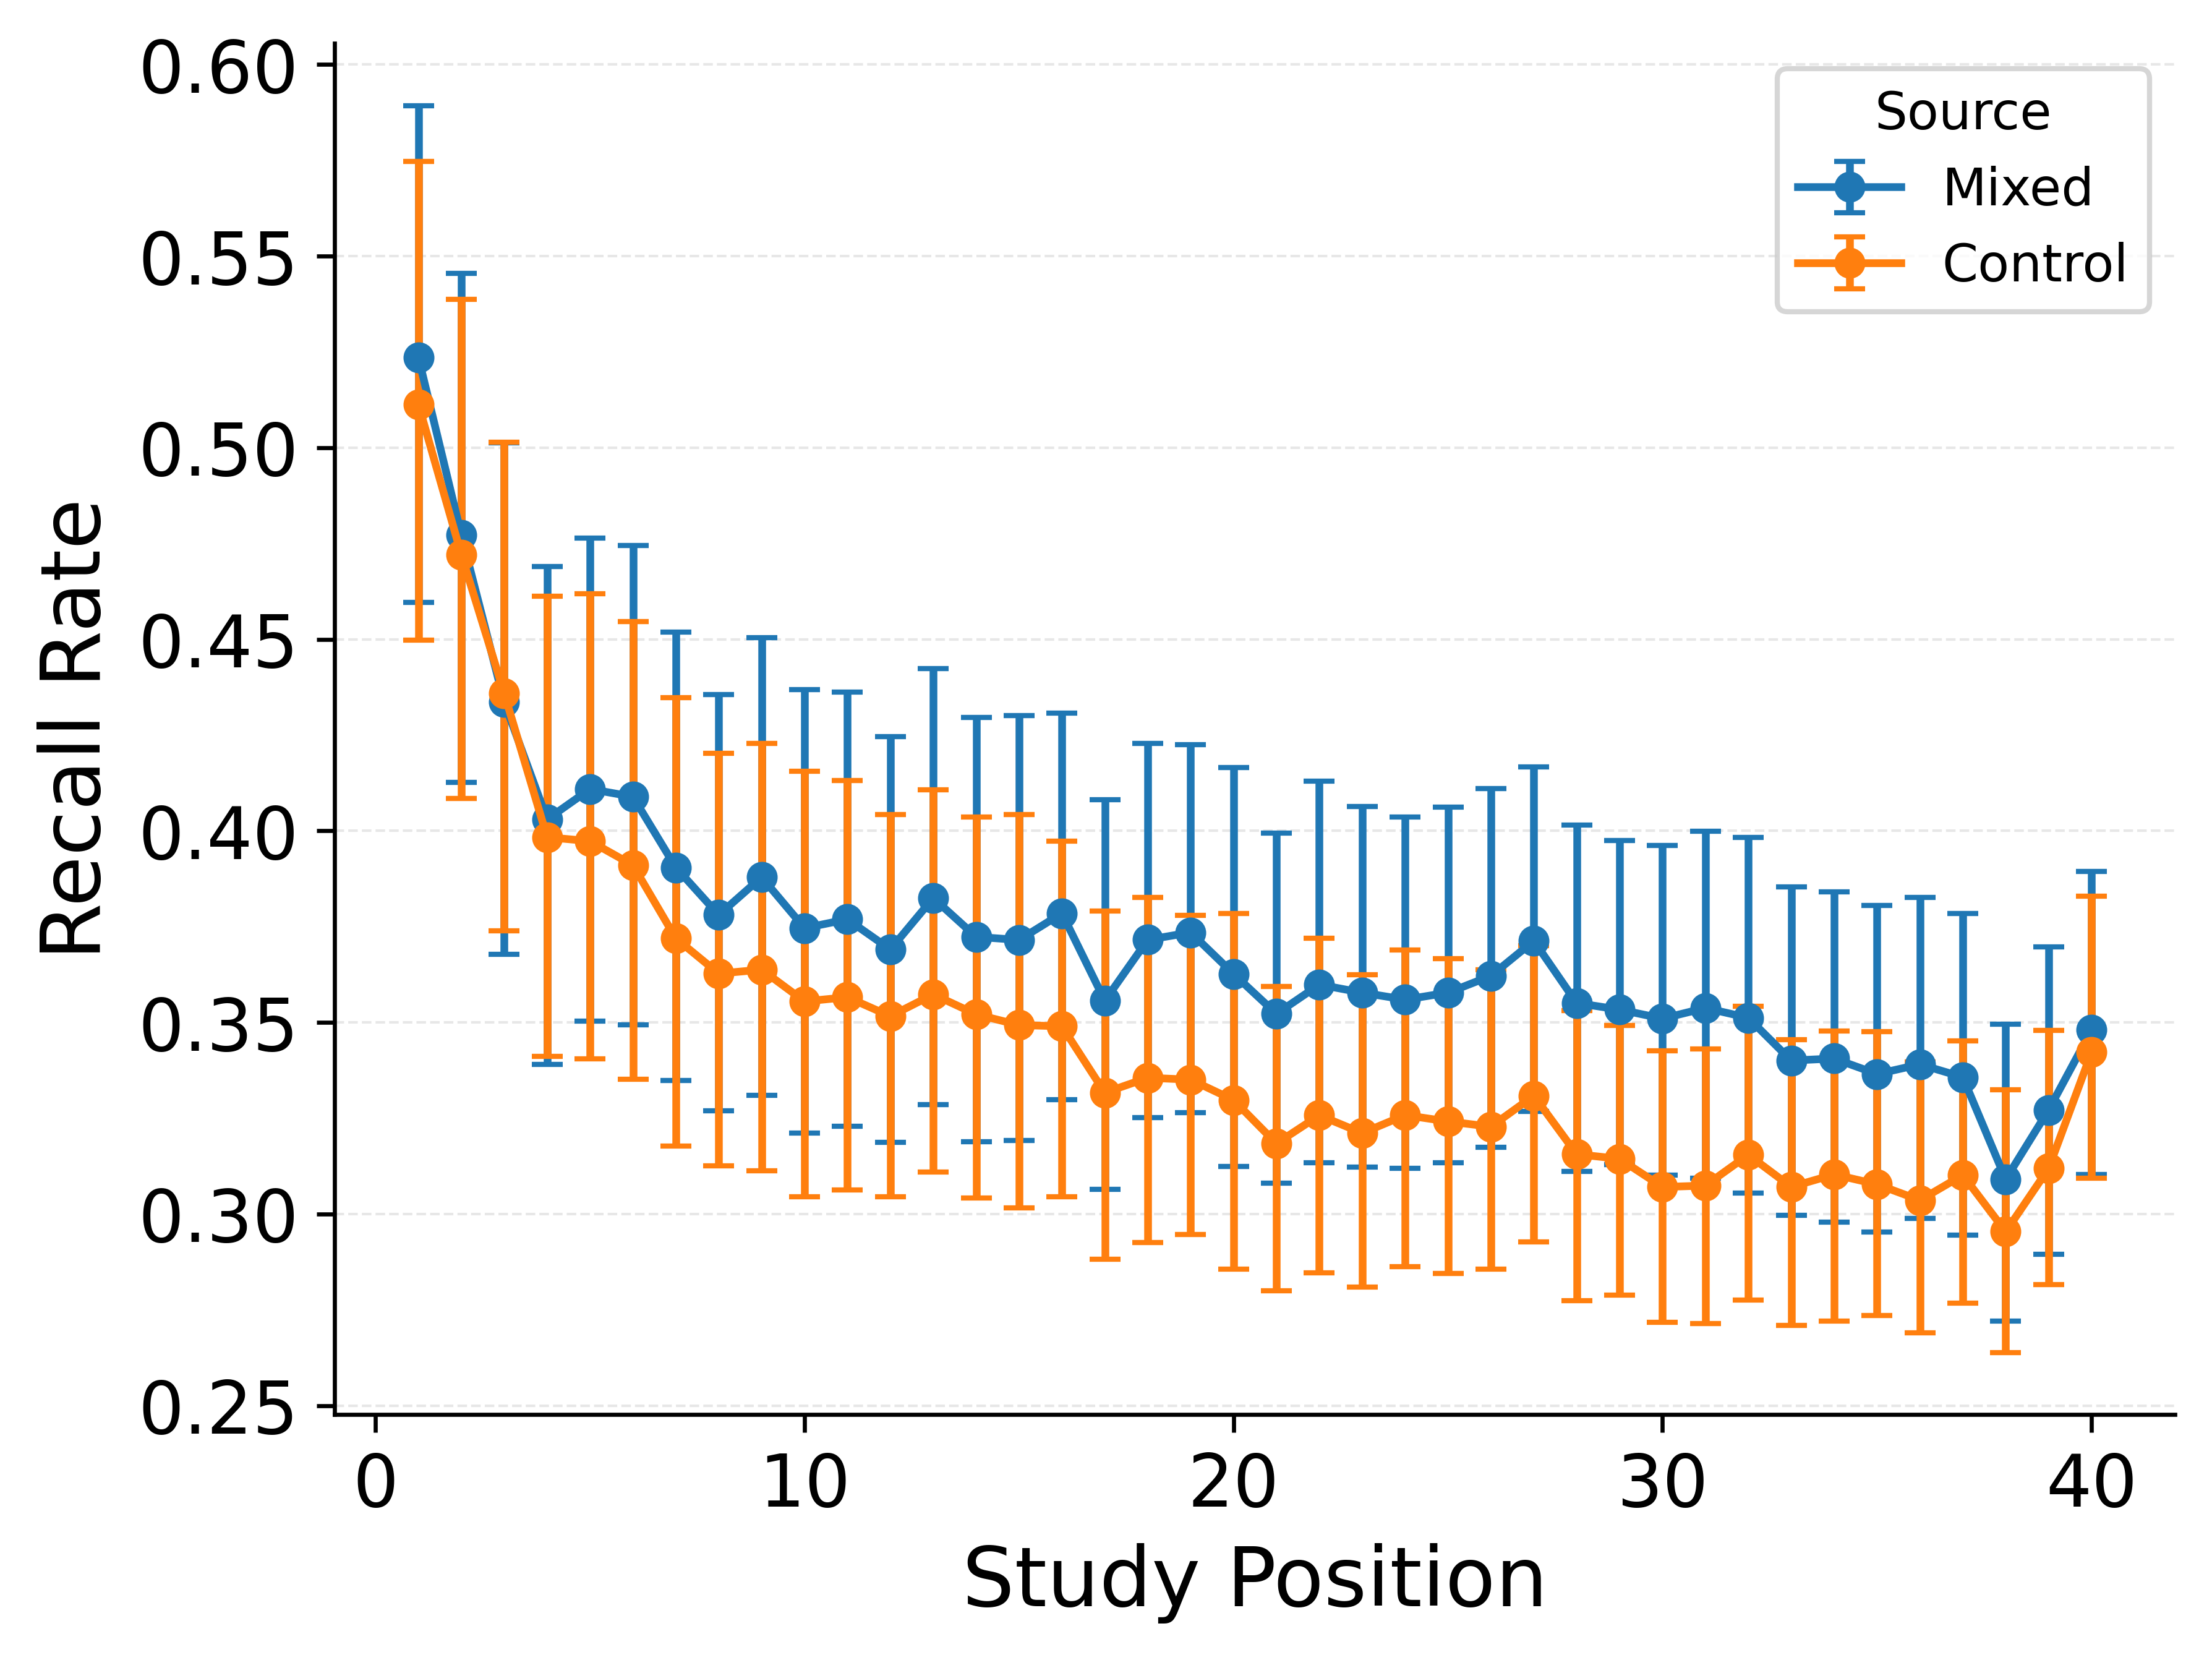
\includegraphics{../../work/thesis/figures/LohnasKahana2014_mixedvscontrolA_WeirdCMRDistinctContexts_full_best_of_3_LT4_spc.png}\end{minipage}%
%
\begin{minipage}{0.50\linewidth}
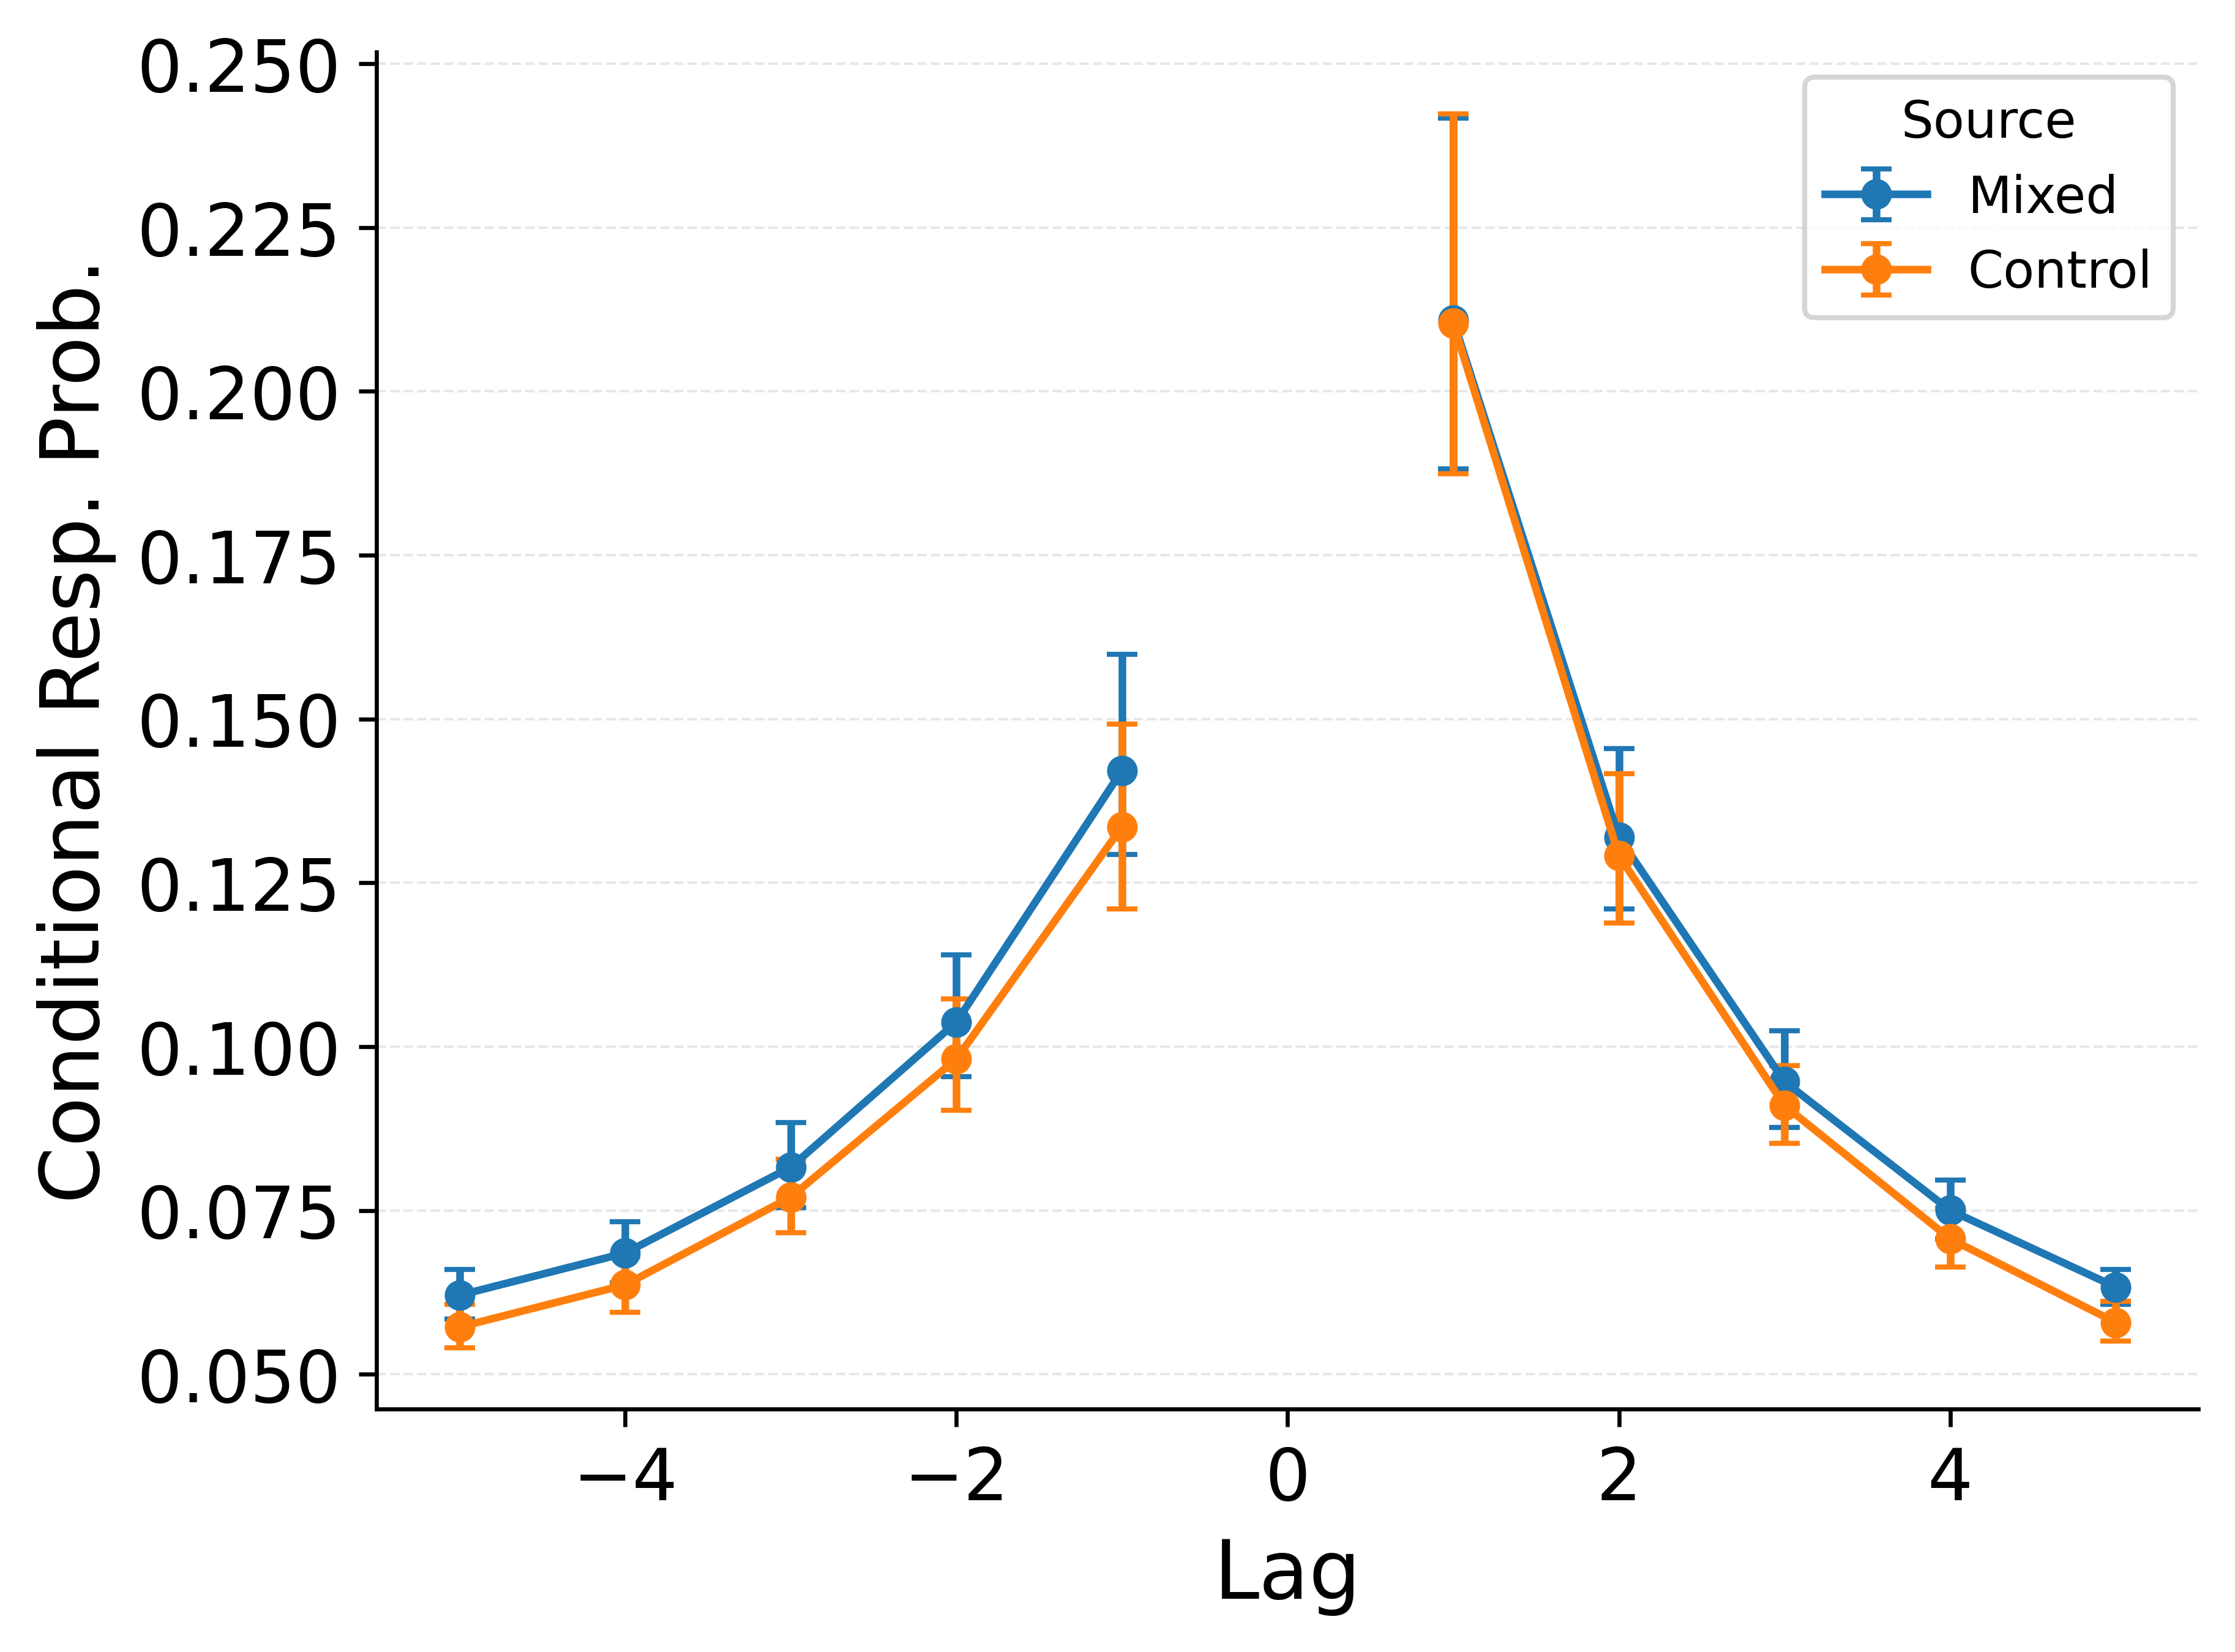
\includegraphics{../../work/thesis/figures/LohnasKahana2014_mixedvscontrolA_WeirdCMRDistinctContexts_full_best_of_3_LT4_crp.png}\end{minipage}%
\newline
\begin{minipage}{\linewidth}
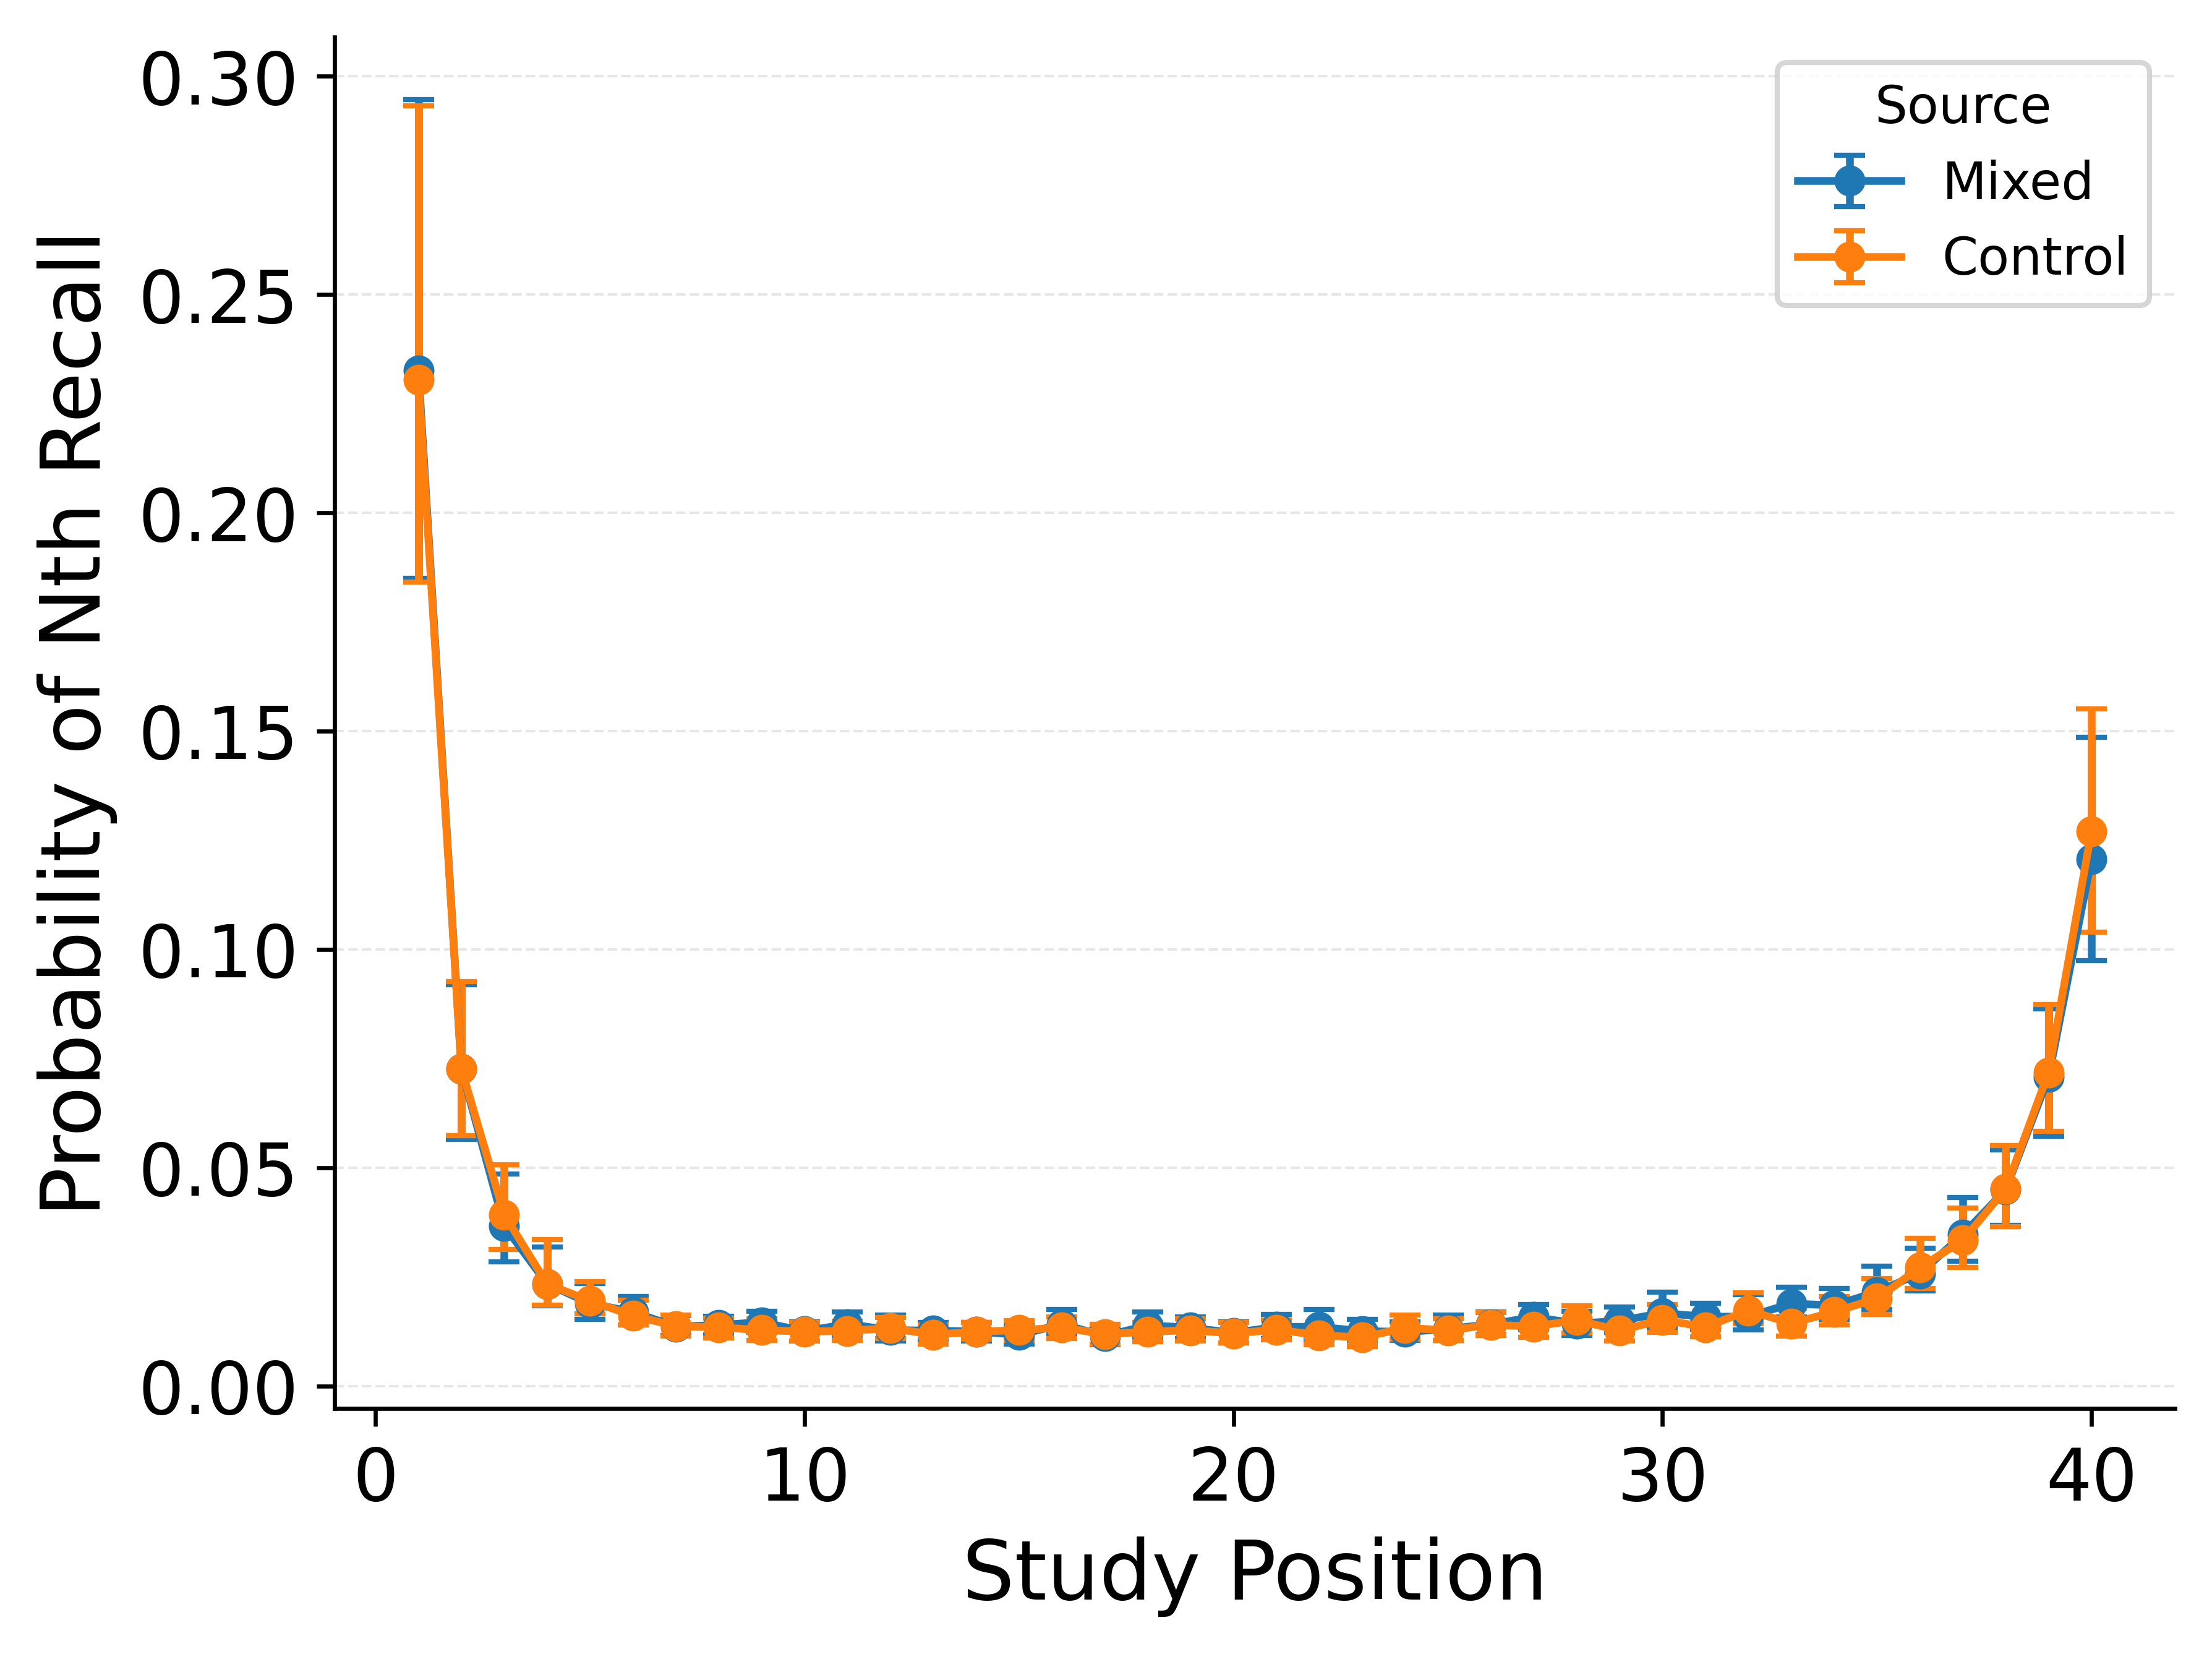
\includegraphics{../../work/thesis/figures/LohnasKahana2014_mixedvscontrolA_WeirdCMRDistinctContexts_full_best_of_3_LT4_pnr.png}\end{minipage}%

\end{figure}%

Critically, removing study-phase reinstatement does not weaken the
spacing function relative to standard CMR fits (cf.
Figure~\ref{fig-spacing}). This indicates that, in these list-learning
paradigms, contextual variability plus test-phase reinstatement is
sufficient to generate the spacing effect at least to the extent
realized by the model; the particular form of study-phase reinstatement
implemented in standard CMR is not required.

\begin{figure}

\caption{\label{fig-nospr_spacing}CMR-NoSPR spacing function. Simulated
spacing curves for mixed vs matched-control lists from Lohnas and Kahana
(\citeproc{ref-lohnas2014retrieved}{2014}). The spacing advantage is
preserved without study-phase reinstatement.}

\begin{minipage}{0.50\linewidth}

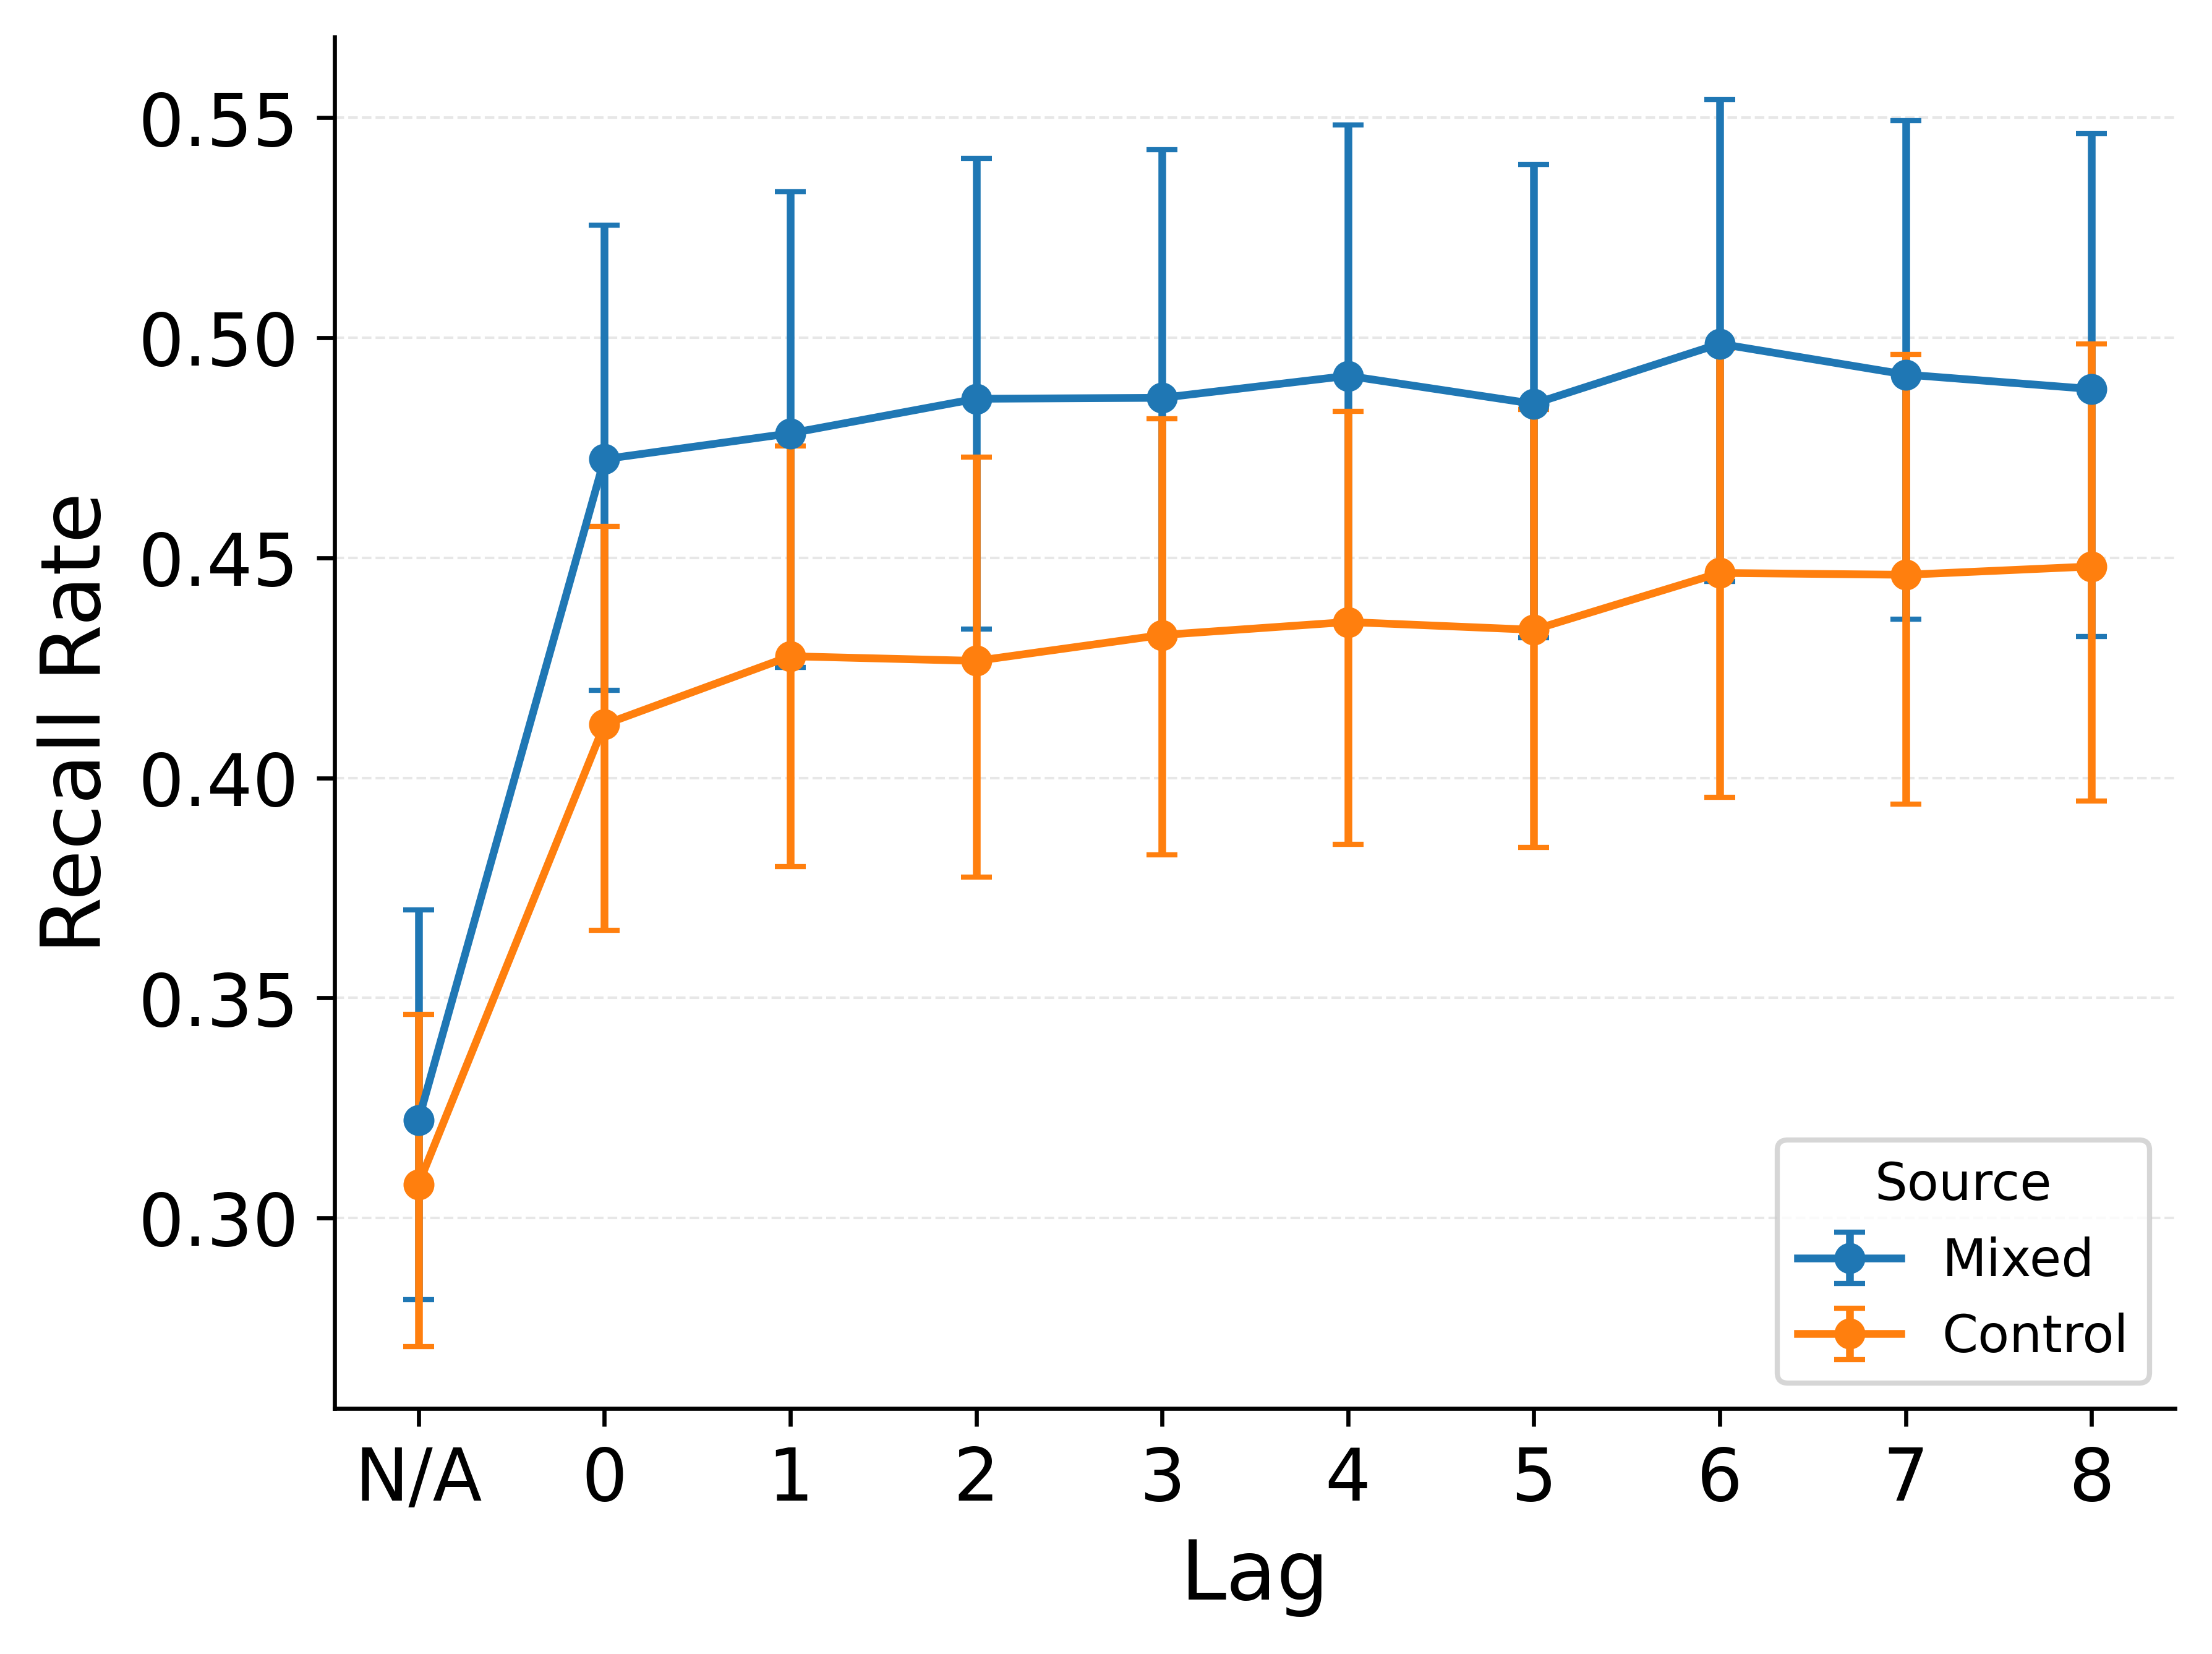
\includegraphics{../../work/thesis/figures/LohnasKahana2014_mixedvscontrolA_WeirdCMRDistinctContexts_full_best_of_3_LT4_full_rpl.png}

\end{minipage}%

\end{figure}%

Next we turn to cross-occurrence neighbor contiguity. Here CMR-NoSPR
achieves the data's non-elevation. Because occurrences now encode to
distinct contextual states, the neighborhoods around the two
presentations are not knitted together at study through association to
overlapping contexts. In the centered neighbor-contiguity tests
(triggers from one neighborhood, lags centered on the other),
mixed--minus--baseline curves sit at baseline in both directions
relative to the other occurrence's neighbors in both trigger directions,
eliminating the cross-occurrence neighbor peaks predicted by standard
CMR (Figure~\ref{fig-nospr_neighbor_contiguity}). This shows the
original neighbor-contiguity elevation is a signature of study-phase
knitting.

\begin{figure}

\caption{\label{fig-nospr_neighbor_contiguity}CMR-NoSPR:
cross-occurrence neighbor transitions (centered lag-CRPs). Left:
triggers from forward neighbors of the first presentation and lags
centered on the second. Right: triggers from forward neighbors of the
second and lags centered on the first. Curves plot
mixed--minus--matched-control probabilities with symmetric scoring. With
distinctive encoding contexts, cross-occurrence neighbor bins lie at
baseline in both directions---neighbor knitting is abolished.}

\begin{minipage}{0.50\linewidth}
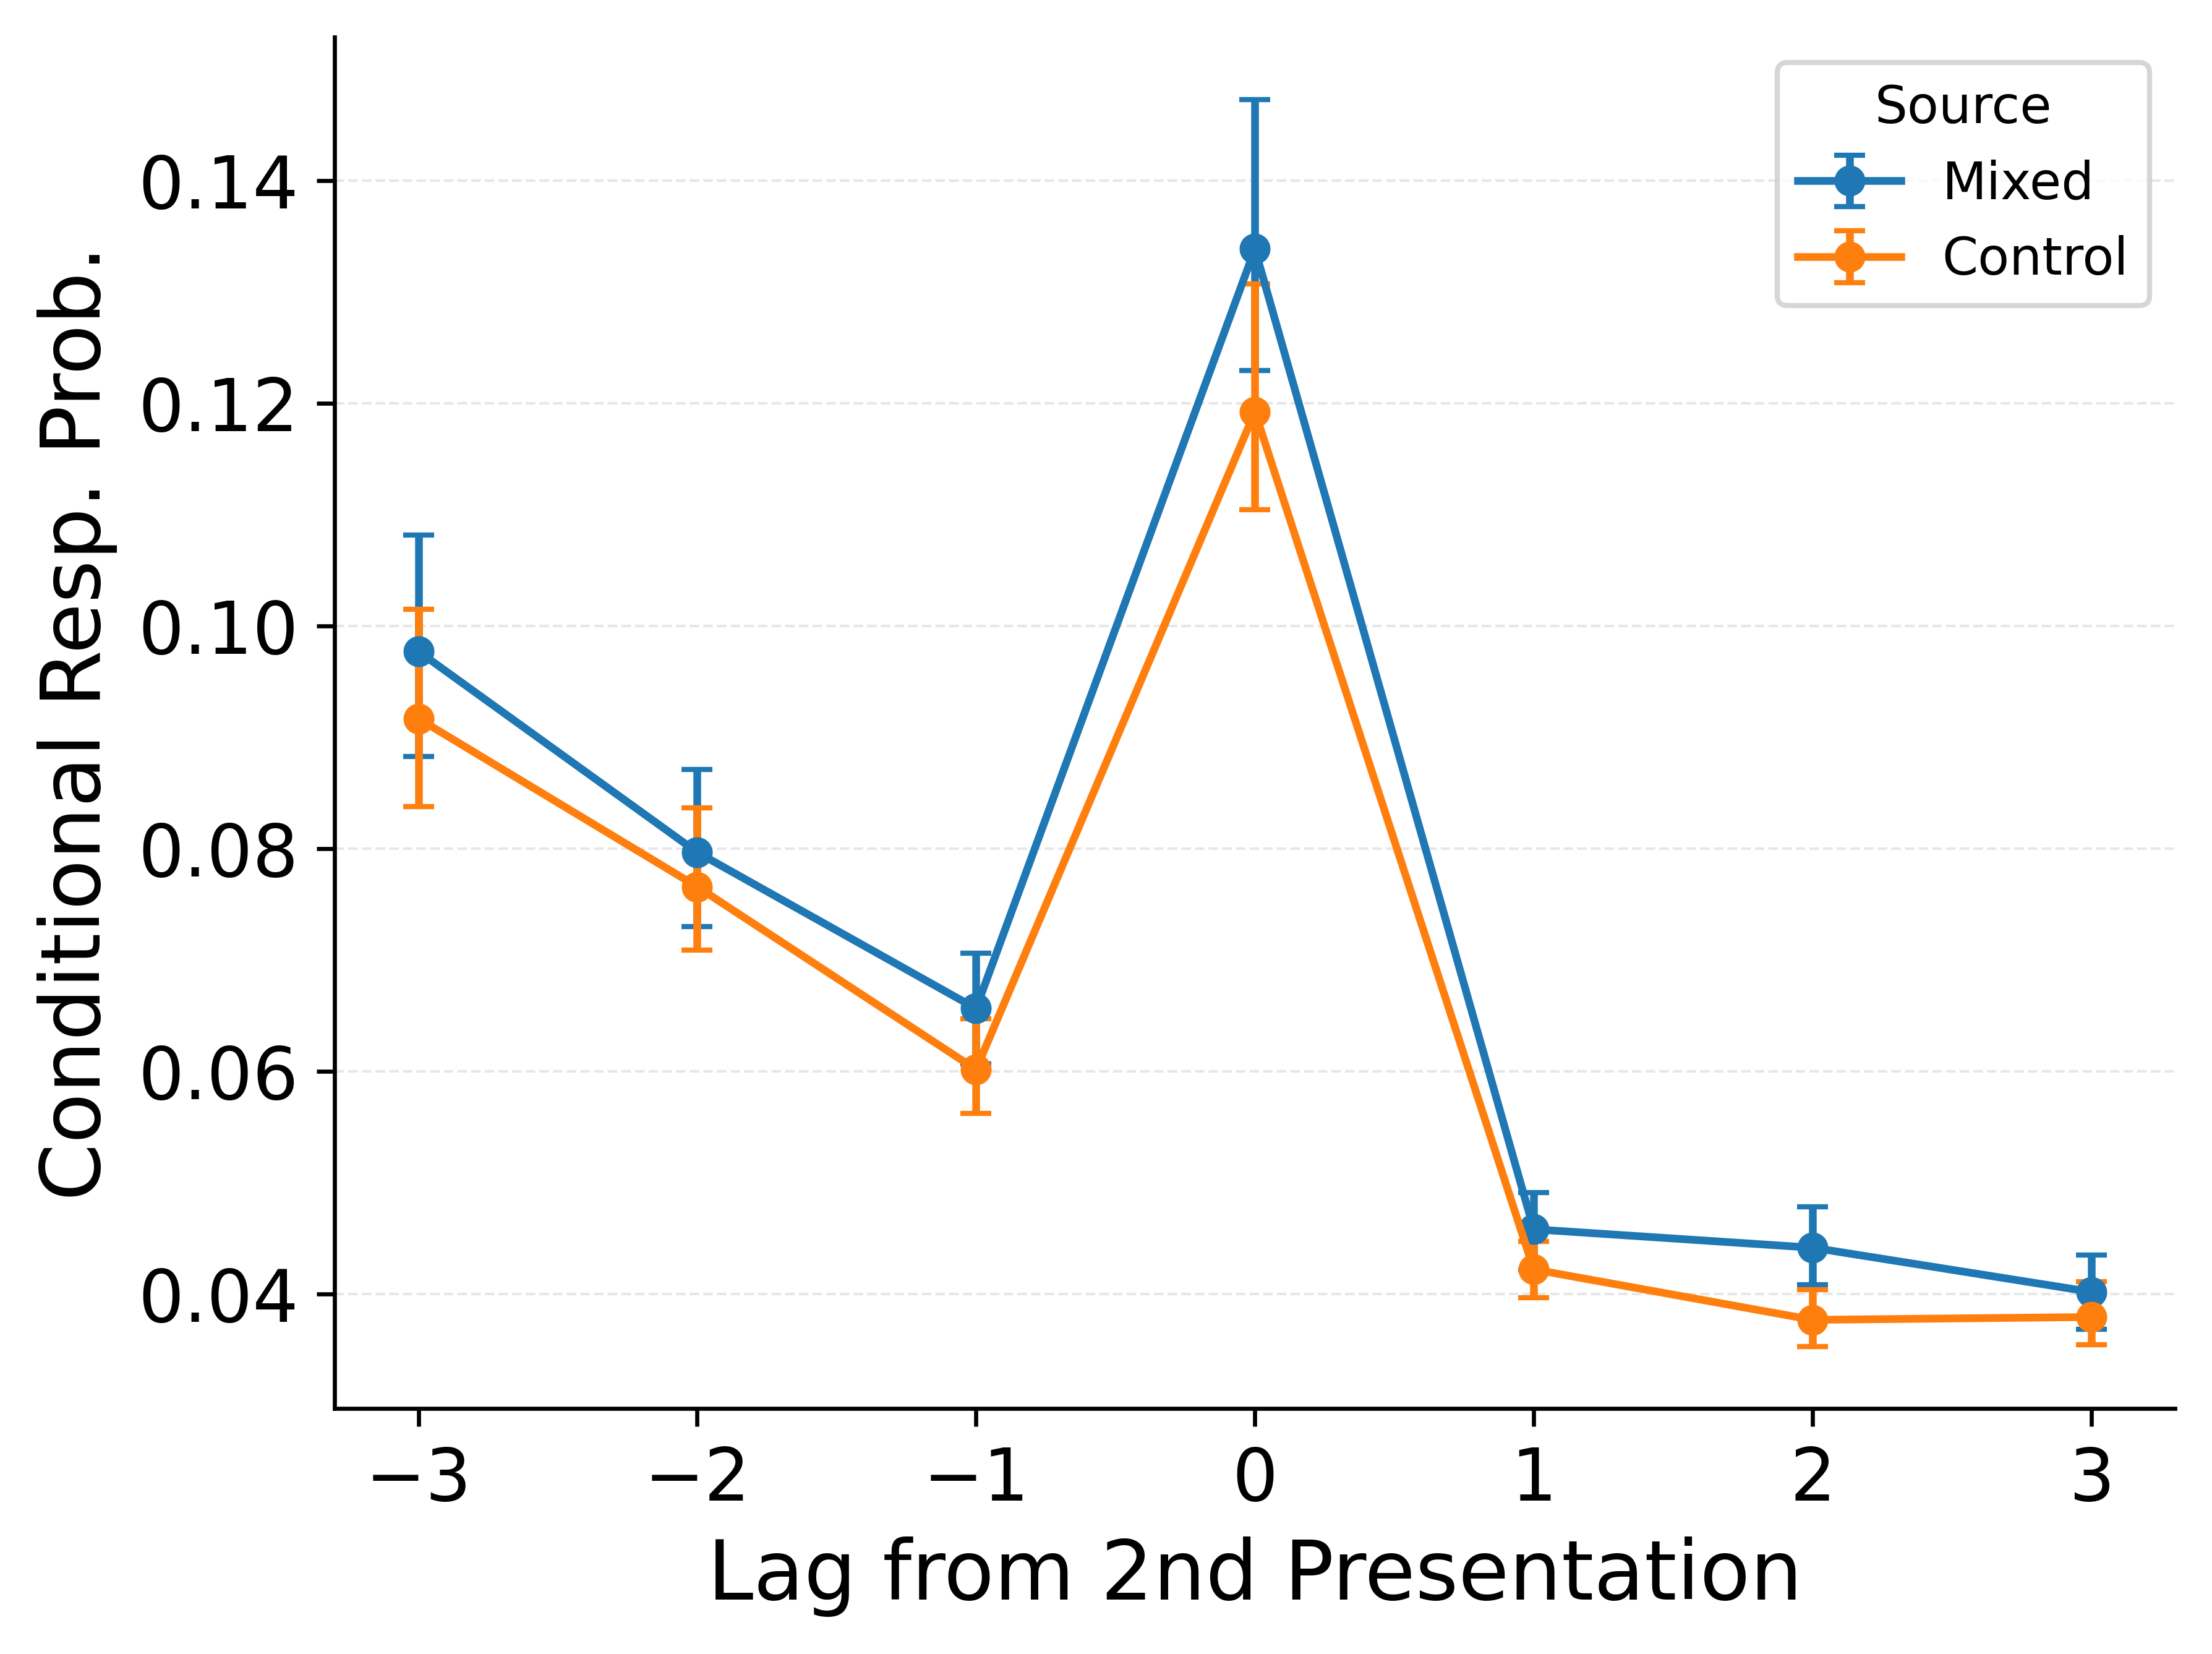
\includegraphics{../../work/thesis/figures/LohnasKahana2014_mixedvscontrolA_WeirdCMRDistinctContexts_full_best_of_3_LT4_repneighborcrp_i2j.png}\end{minipage}%
%
\begin{minipage}{0.50\linewidth}
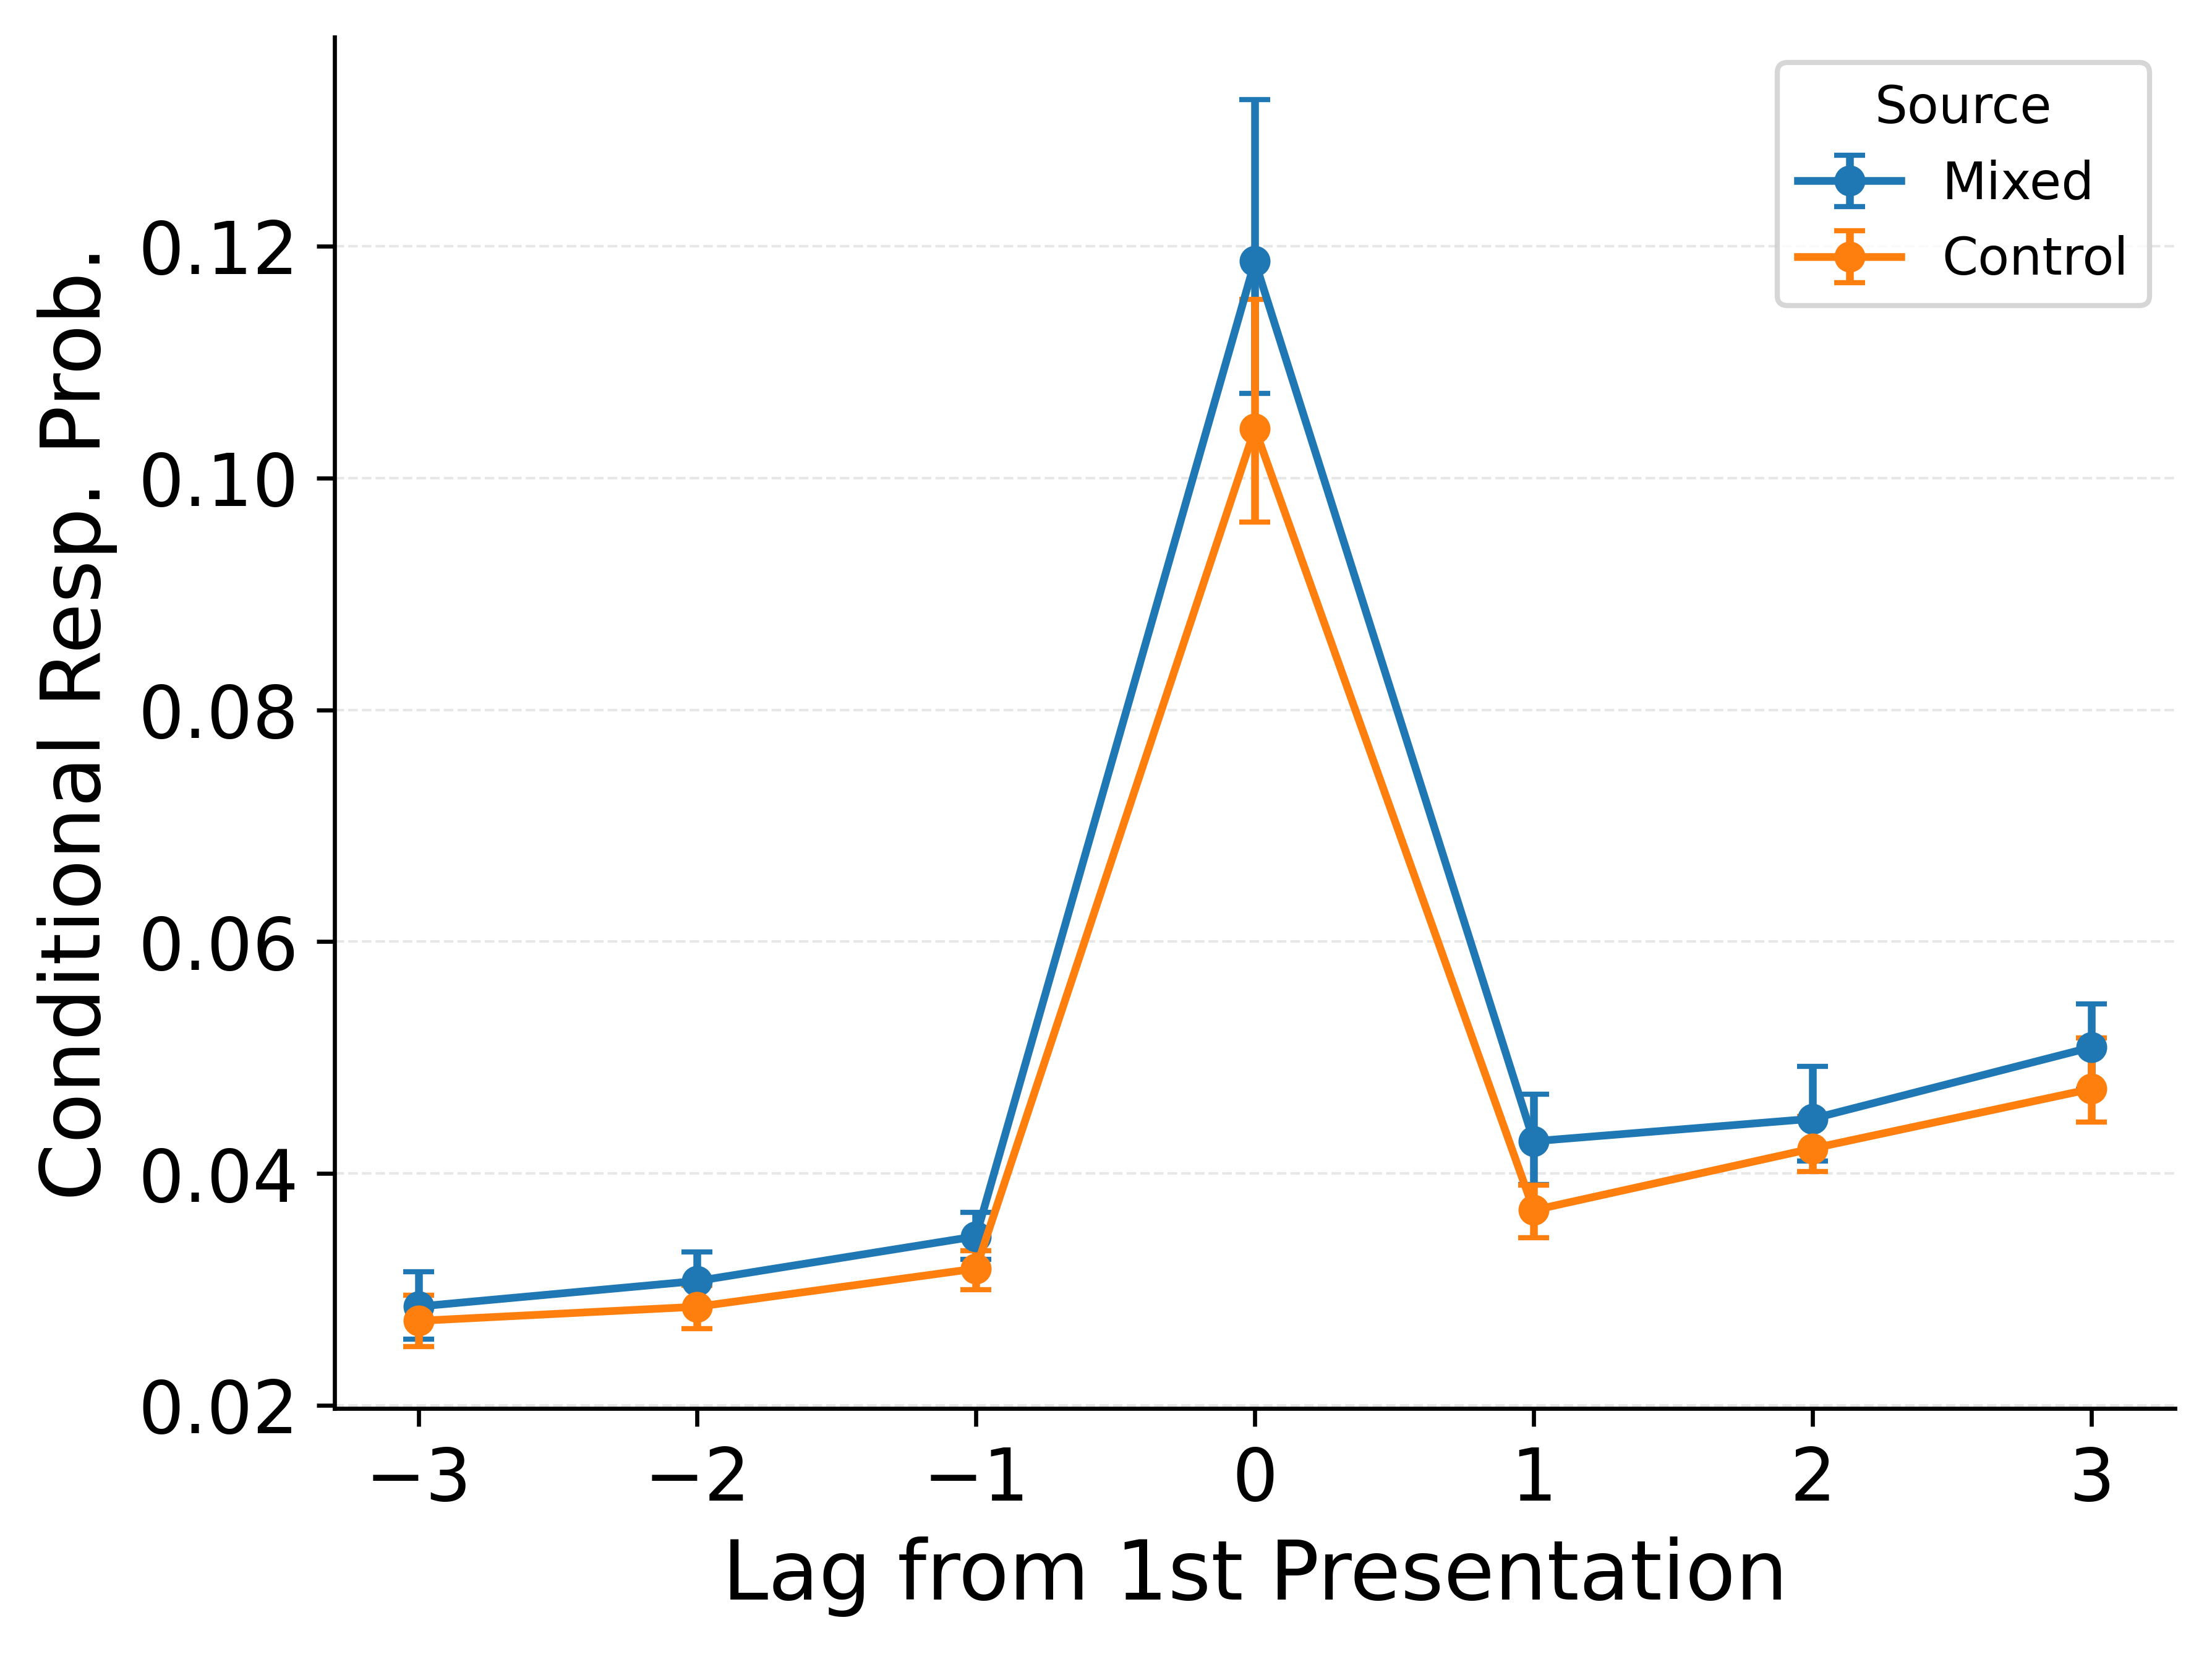
\includegraphics{../../work/thesis/figures/LohnasKahana2014_mixedvscontrolA_WeirdCMRDistinctContexts_full_best_of_3_LT4_repneighborcrp_j2i.png}\end{minipage}%

\end{figure}%

On the other hand, the outgoing repetition lag-CRP still shows the
balanced-access signature of associative interference: transitions from
a recalled repeater distribute more evenly to the two neighborhoods than
in the matched baseline (Figure~\ref{fig-nospr_rep_lag_crp}).
Eliminating study-phase reinstatement therefore does not restore the
first-over-second advantage seen in the data (cf.
Figure~\ref{fig-repetition_lag_crp}); the repeater still reinstates a
composite cue that contacts both occurrence contexts.

\begin{figure}

\caption{\label{fig-nospr_rep_lag_crp}CMR-NoSPR: repetition lag-CRP
(outgoing). Mixed lists (left) and matched-control baseline (right) from
simulations. First- vs second-centered curves are more balanced than in
baseline, consistent with lingering cross-occurrence blending at
retrieval.}

\begin{minipage}{0.50\linewidth}
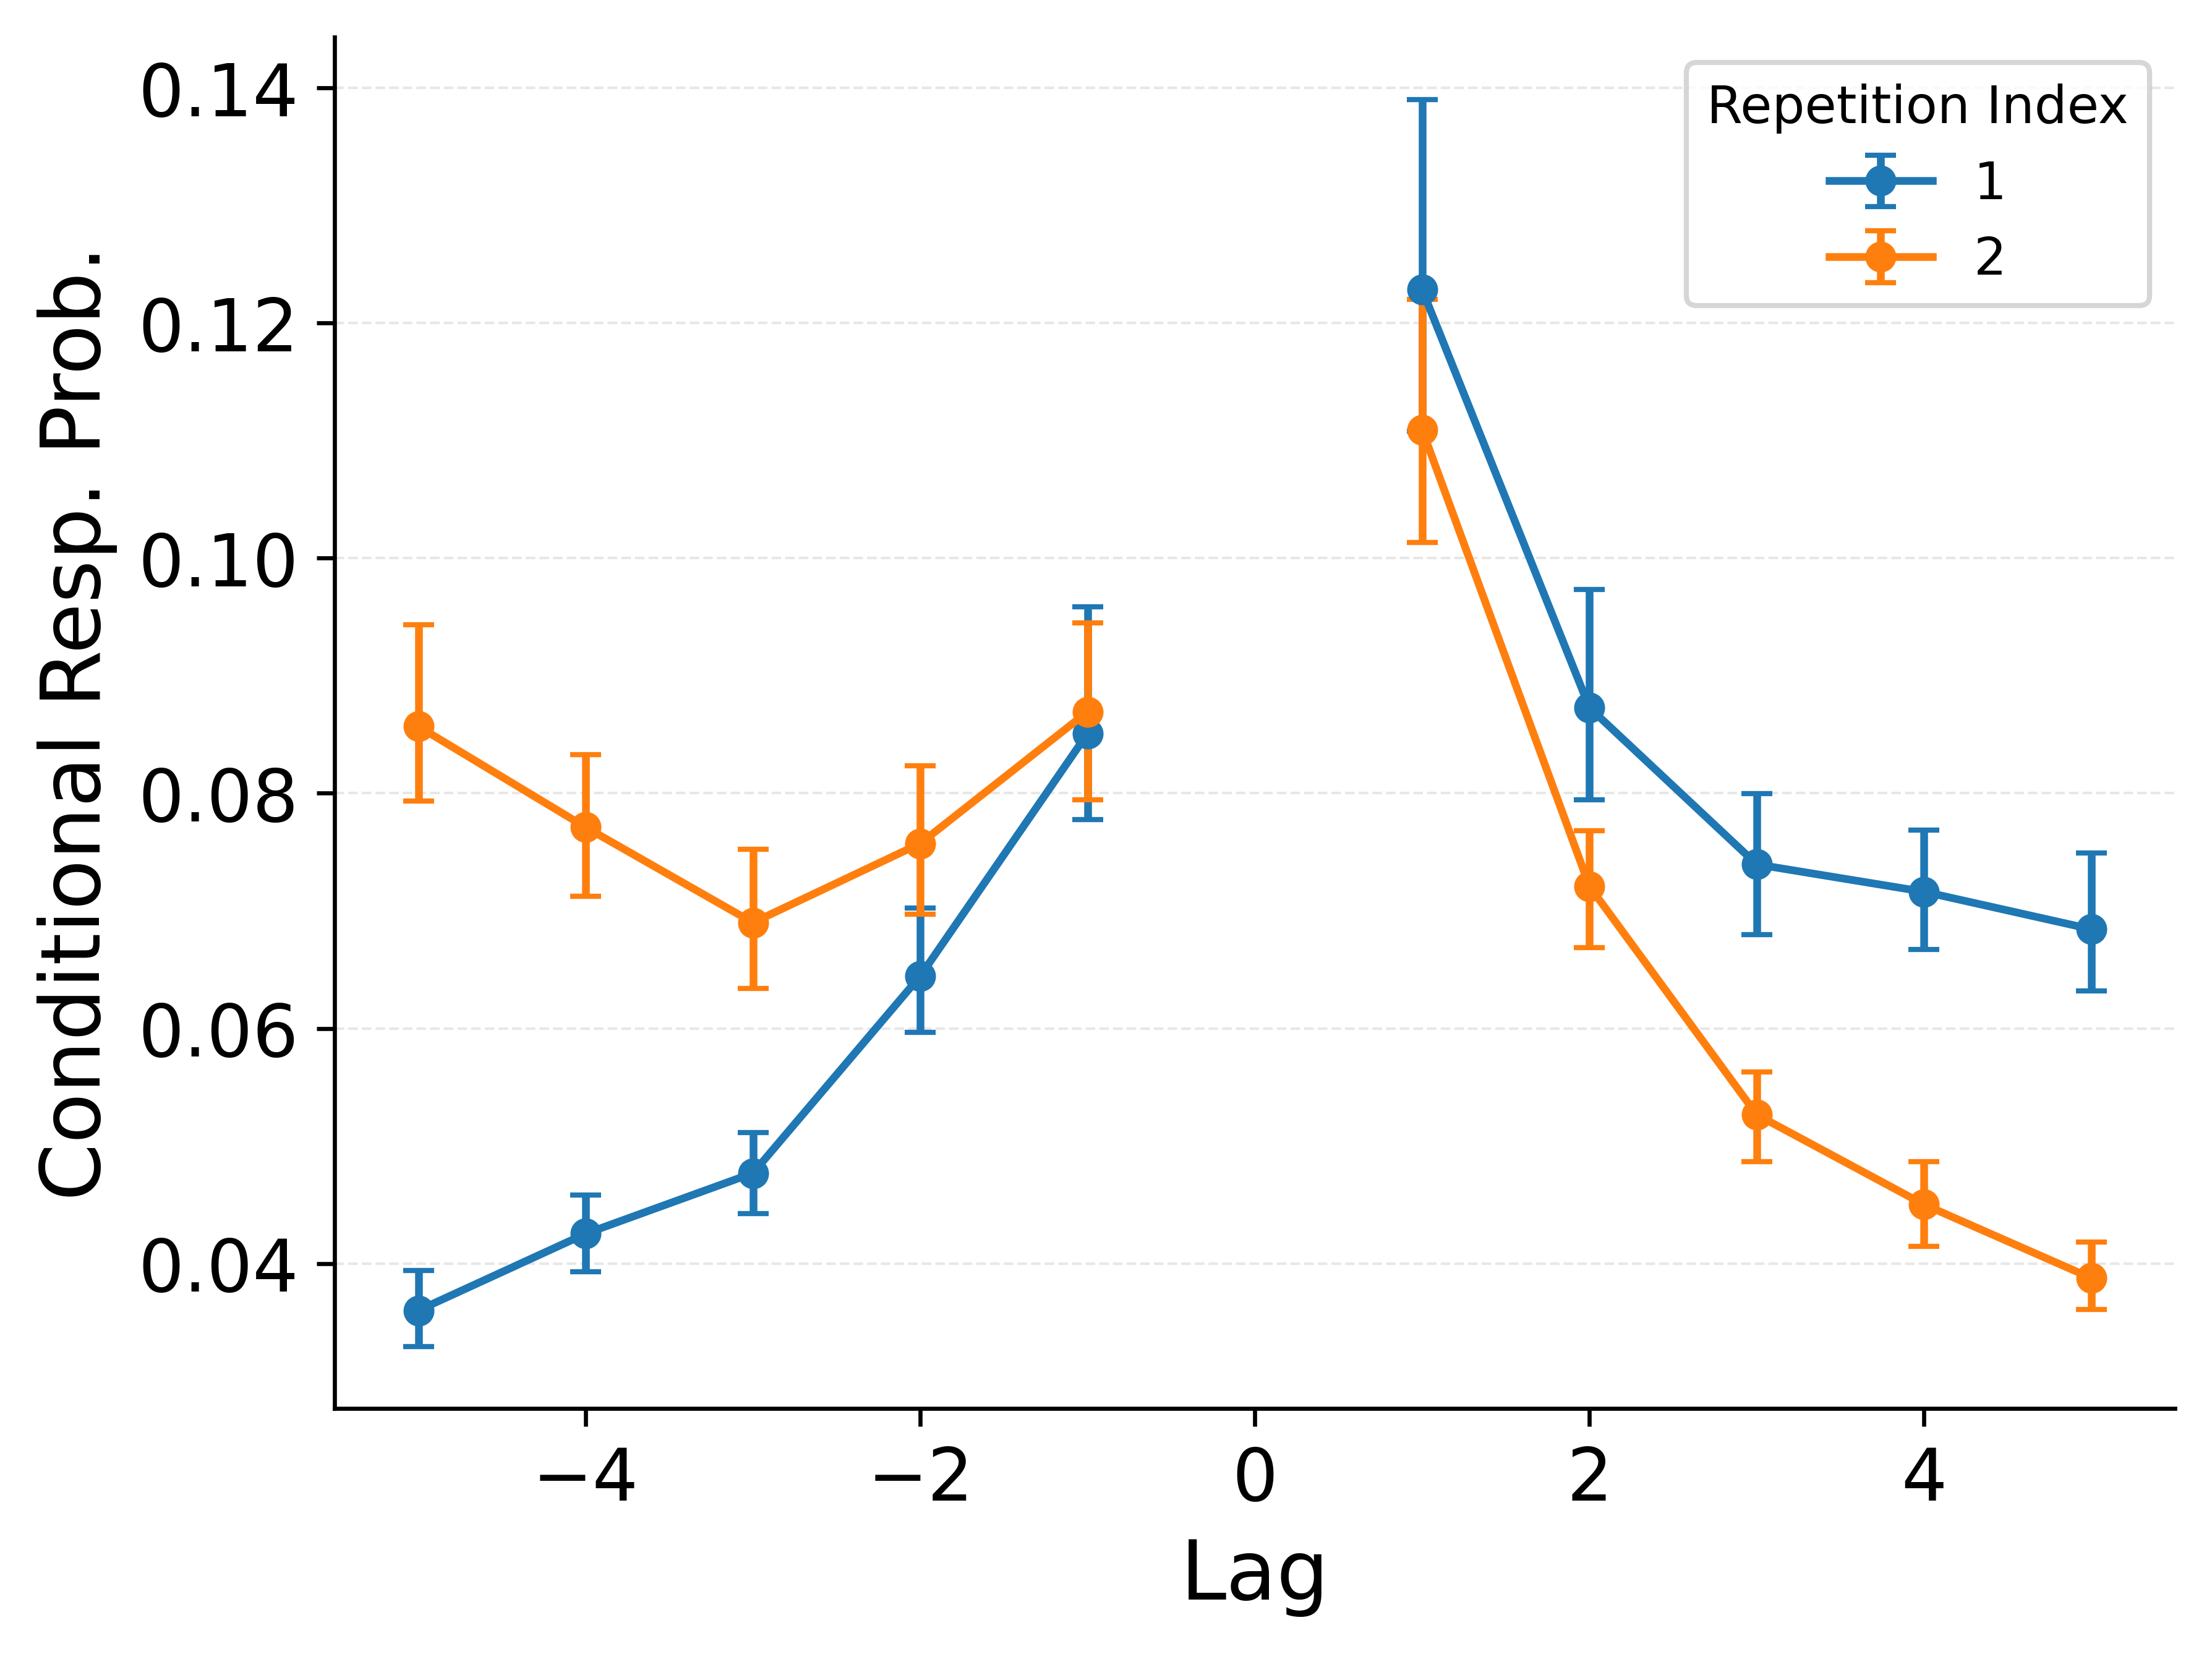
\includegraphics{../../work/thesis/figures/LohnasKahana2014_mixed_WeirdCMRDistinctContexts_full_best_of_3_LT4_rep_crp.png}\end{minipage}%
%
\begin{minipage}{0.50\linewidth}
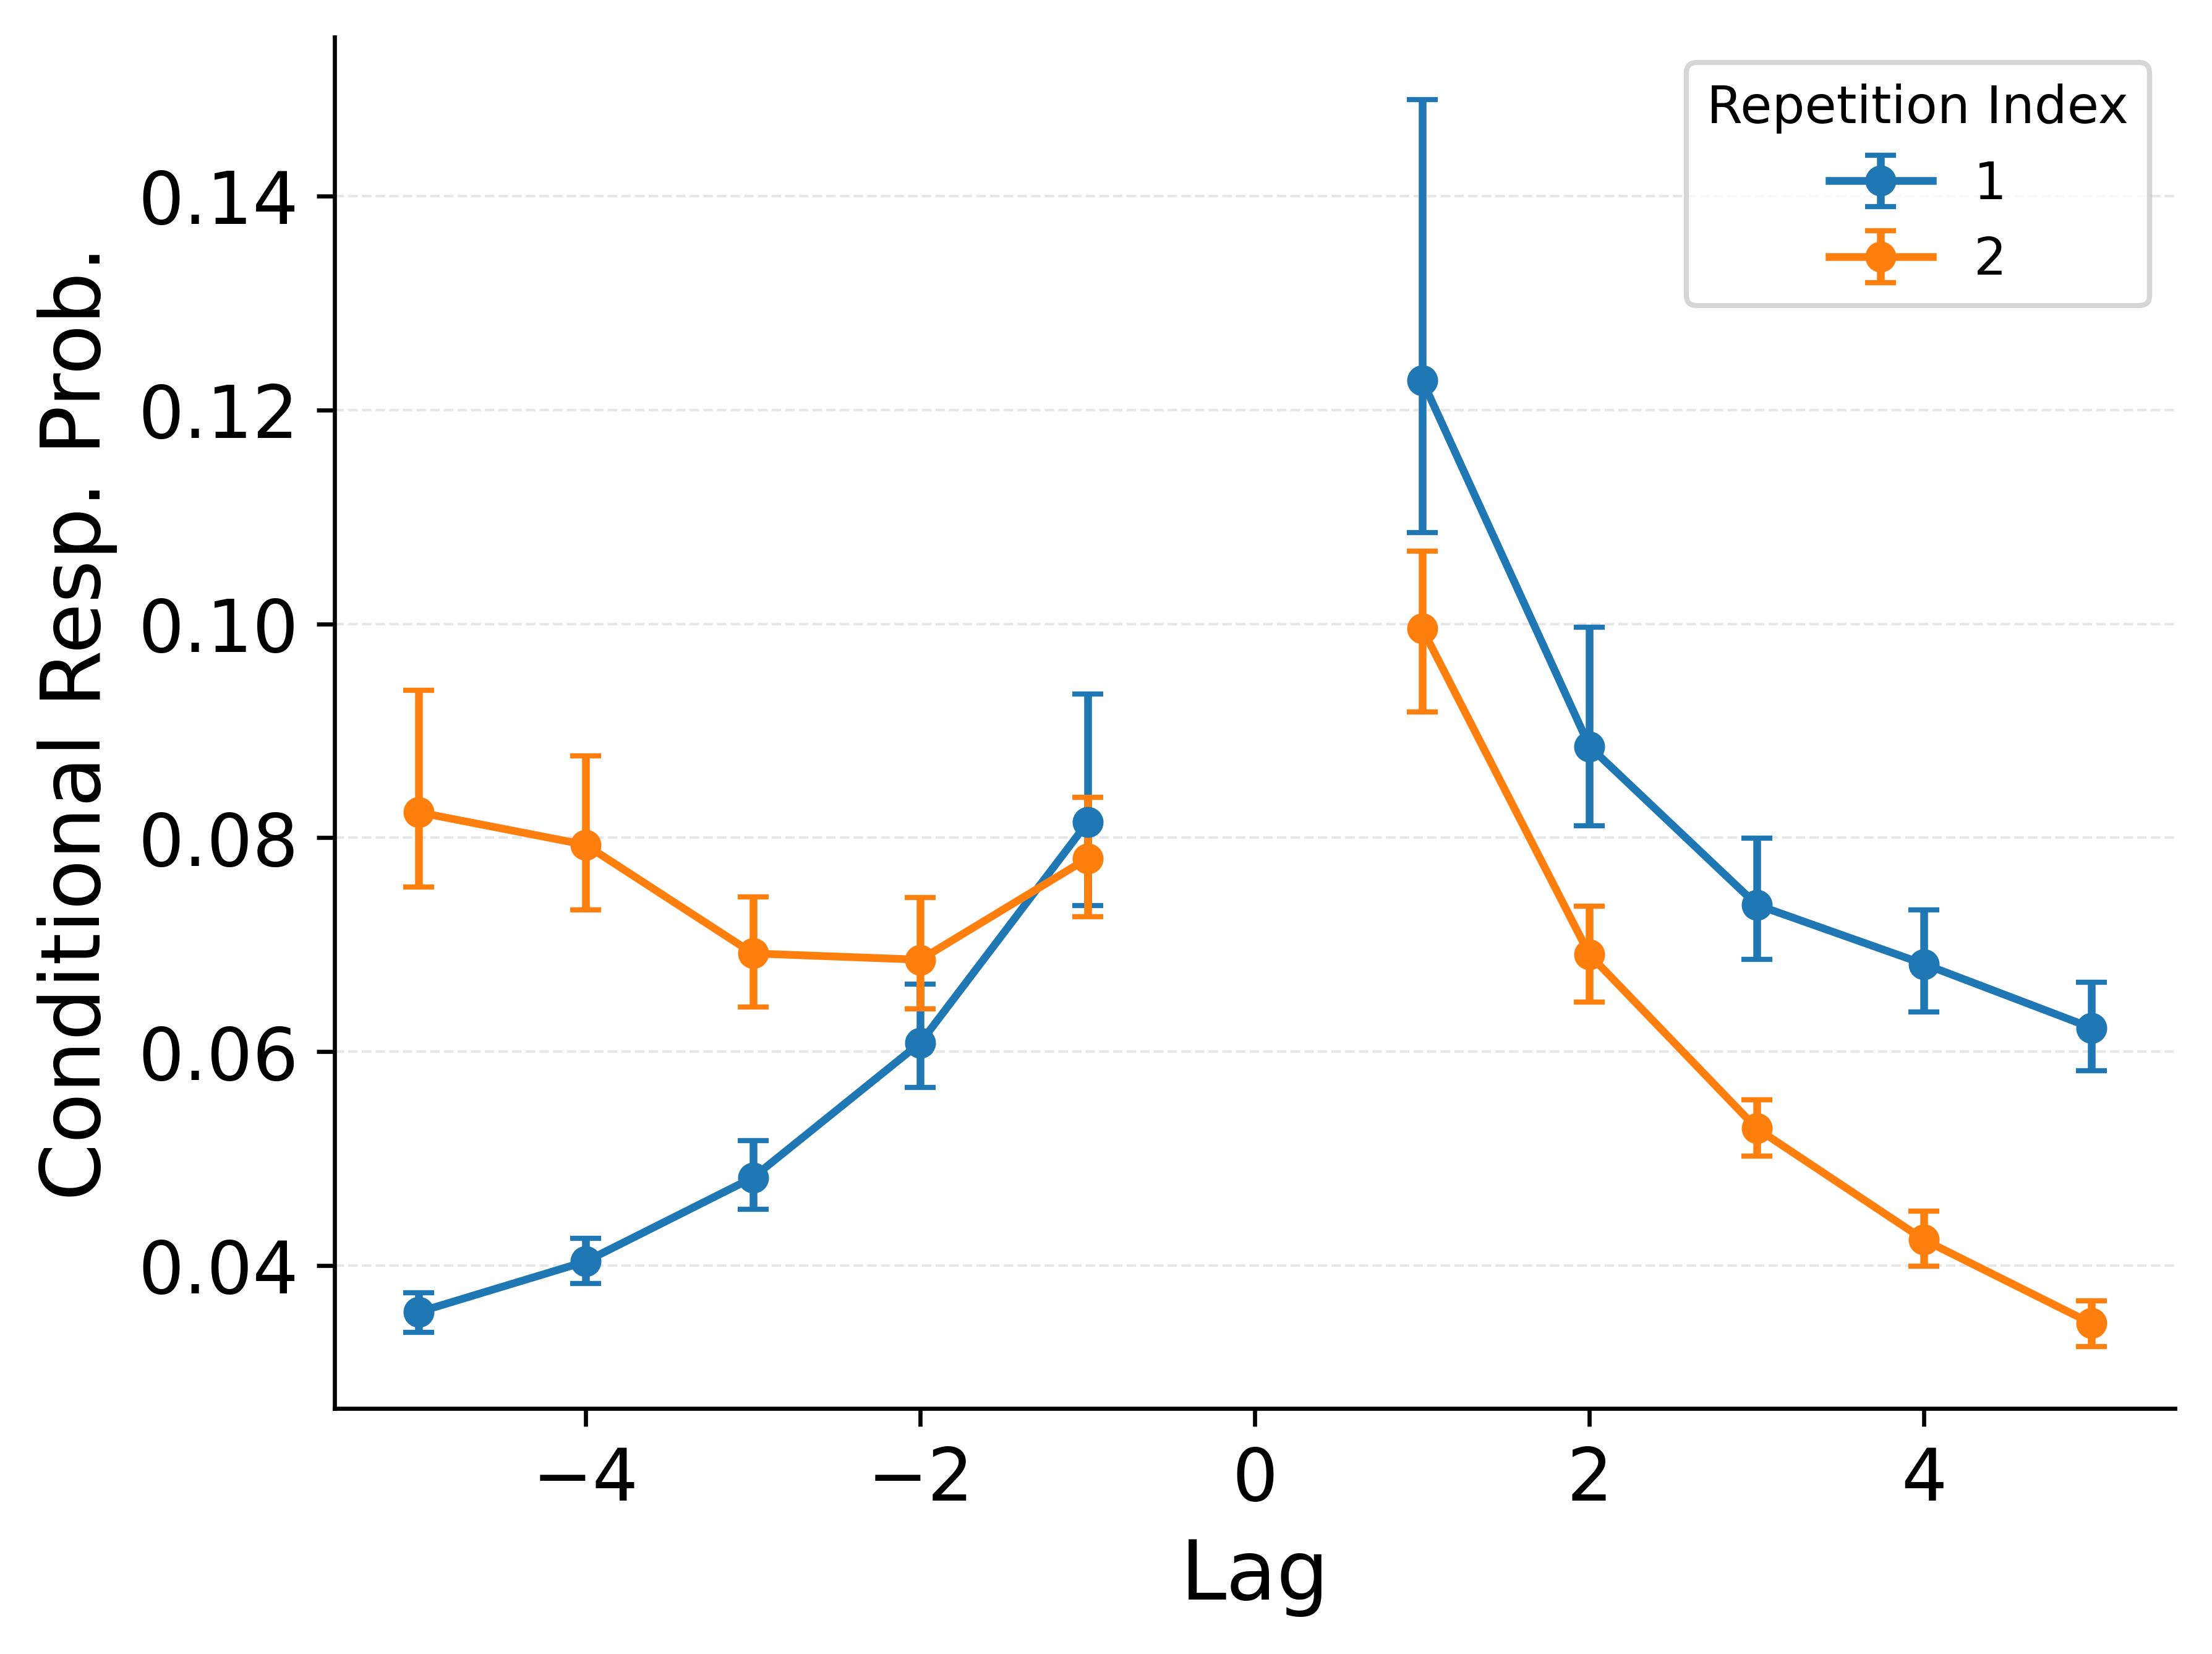
\includegraphics{../../work/thesis/figures/LohnasKahana2014_control_WeirdCMRDistinctContexts_full_best_of_3_LT4_rep_crp.png}\end{minipage}%

\end{figure}%

CMR-NoSPR demonstrates that study-phase reinstatement is not necessary
for the spacing effect or for core free-recall benchmarks, and it
eliminates the cross-occurrence neighbor knitting seen in standard
CMR---aligning with the data on that diagnostic. However, it fails to
resolve the interference observed when the repeater itself is the cue:
the outgoing repetition lag-CRP still shows balanced access across the
two neighborhoods. This isolates the remaining source of the problem to
blending at retrieval, motivating the next step---an occurrence-specific
reinstatement scheme (Instance-CMR) that lets traces compete so recall
can route through one occurrence without contacting the other.

\section{Instance-CMR: Eliminating Associative Interference at Encoding
and
Retrieval}\label{instance-cmr-eliminating-associative-interference-at-encoding-and-retrieval}

Instance-CMR goes beyond CMR-NoSPR by separating occurrences at both
stages. As in CMR-NoSPR, each repetition event encodes to a
non-overlapping contextual state (no knitting at study). At retrieval,
however, Instance-CMR uses the instance architecture to let occurrence
traces compete: when a repeated item is recalled, the model selectively
reinstates the context of a single occurrence rather than a fixed
composite over occurrences. Selection pressure is governed by the same
trace-sensitivity parameter used in the recall competition (no new
degrees of freedom). This change targets the remaining source of
interference isolated in the last section---blending at test---while
keeping temporal-context dynamics and other task mechanisms identical to
the base model. The questions are whether this variant (i) retains
benchmark free-recall behavior and the spacing function, (ii) eliminates
cross-occurrence neighbor knitting (as CMR-NoSPR already did), (iii)
removes the balanced-access signature in the outgoing repetition
lag-CRP, and (iv) avoids cross-occurrence forward errors in serial
recall.

Instance-CMR maintains good agreement with serial-position, lag-CRP, and
first-recall profiles under the same matched, symmetric scoring used
throughout. As with the previous models, mixed versus control
differences are minimal once the baseline is applied
(Figure~\ref{fig-icmr_os_benchmarks}). Thus, introducing
occurrence-specific reinstatement at test does not degrade core
free-recall benchmarks.

\begin{figure}

\caption{\label{fig-icmr_os_benchmarks}Instance-CMR benchmarks (free
recall). Simulated serial-position curves (SPC; top left), lag-CRP (top
right), and probability of first/next recall (bottom) for mixed vs
matched-control lists from Lohnas and Kahana
(\citeproc{ref-lohnas2014retrieved}{2014}) under symmetric scoring.
Occurrence-specific reinstatement at test preserves benchmark fits.}

\begin{minipage}{0.50\linewidth}
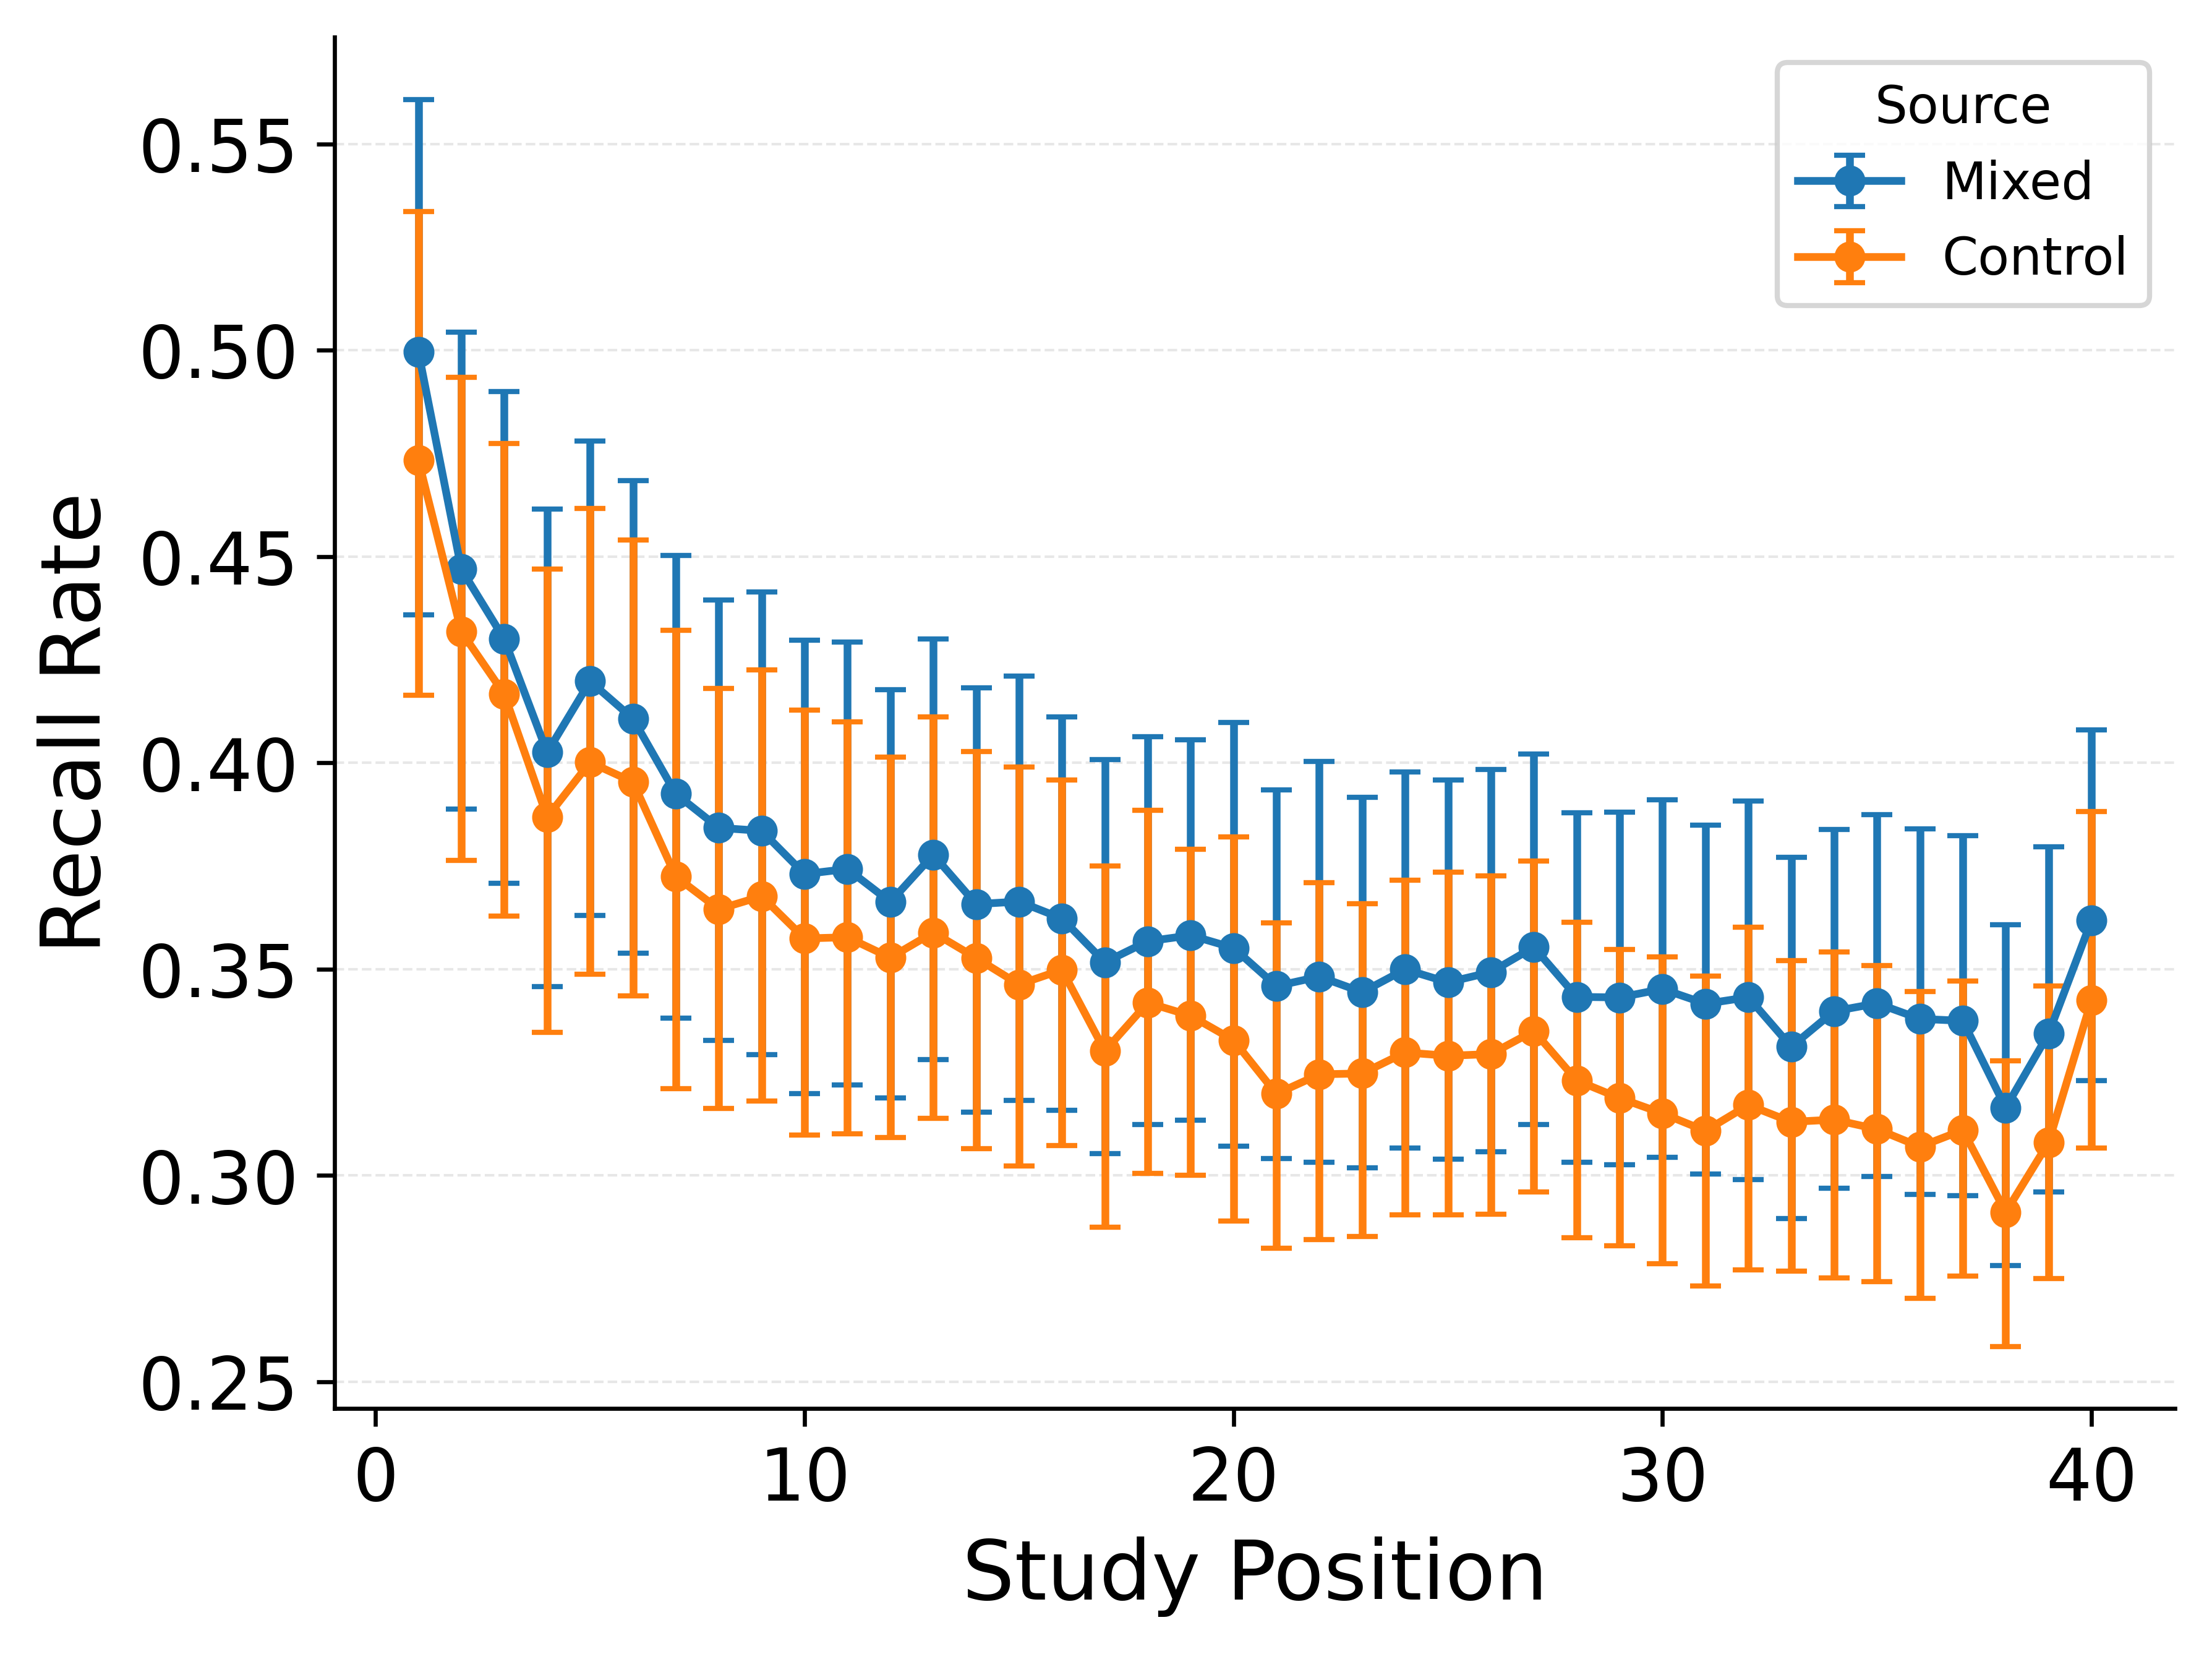
\includegraphics{../../work/thesis/figures/LohnasKahana2014_mixedvscontrolA_WeirdPositionalCMR_full_best_of_3_LT4_spc.png}\end{minipage}%
%
\begin{minipage}{0.50\linewidth}
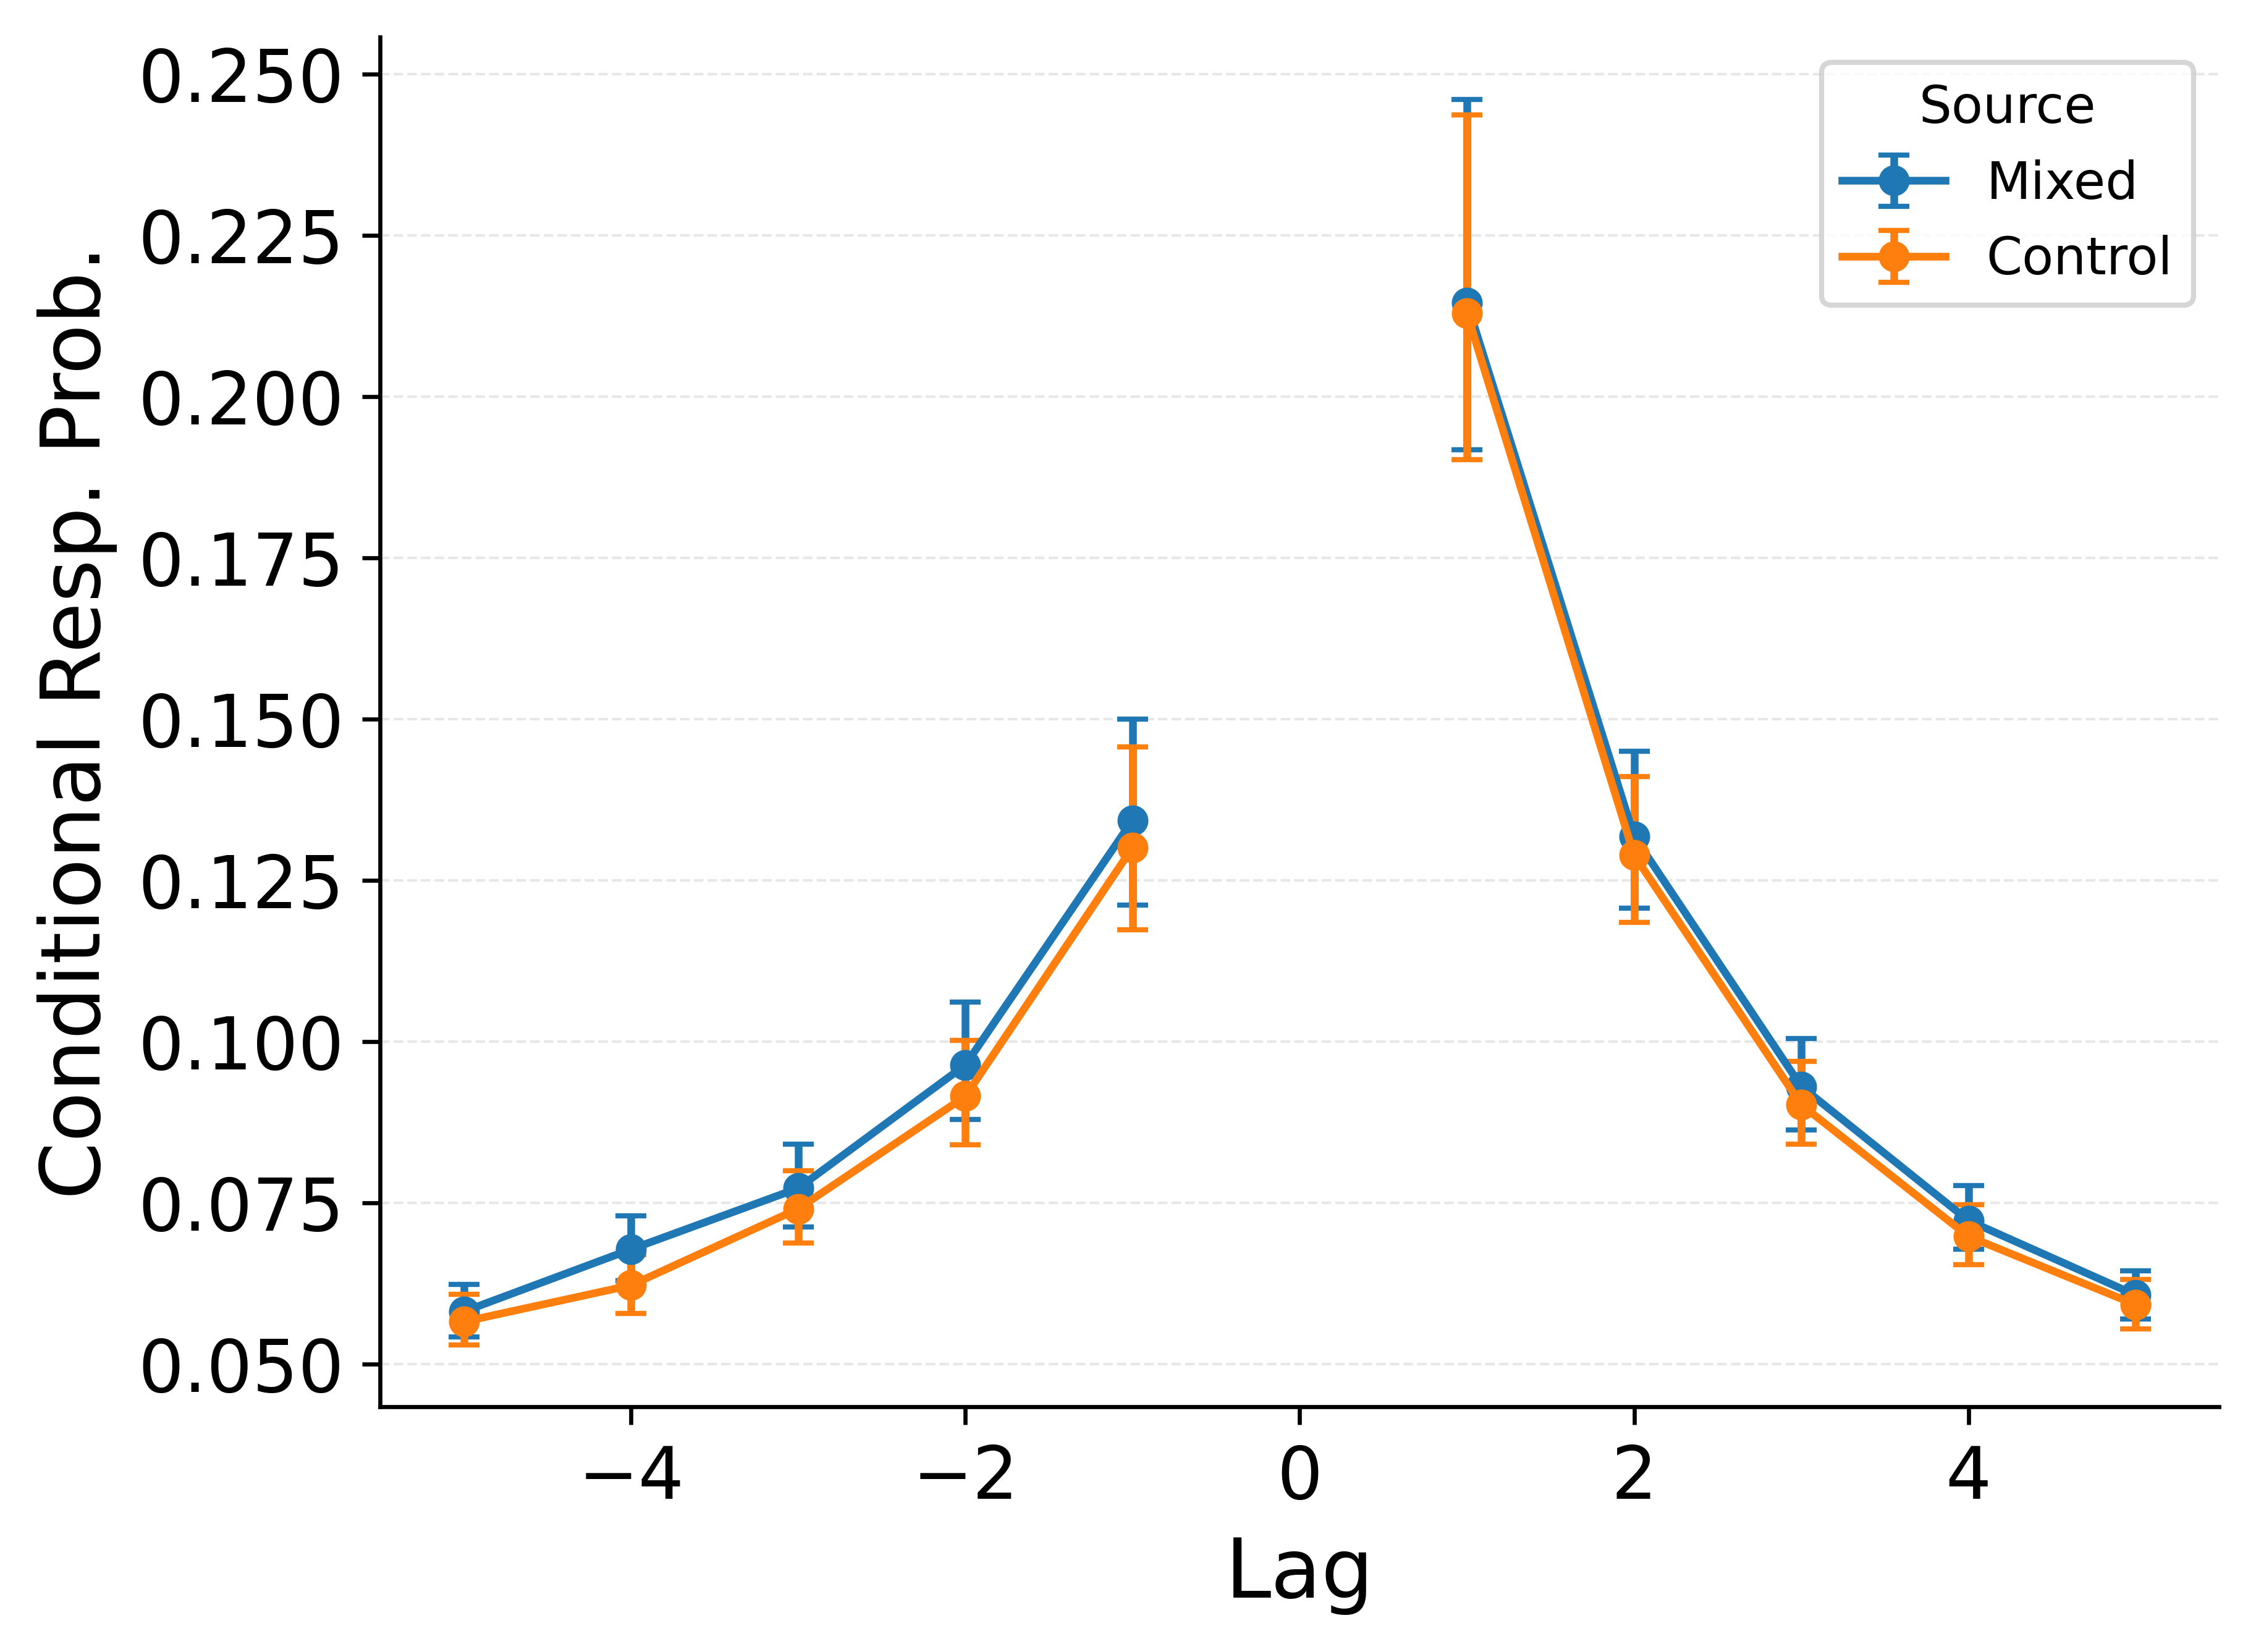
\includegraphics{../../work/thesis/figures/LohnasKahana2014_mixedvscontrolA_WeirdPositionalCMR_full_best_of_3_LT4_crp.png}\end{minipage}%
\newline
\begin{minipage}{\linewidth}
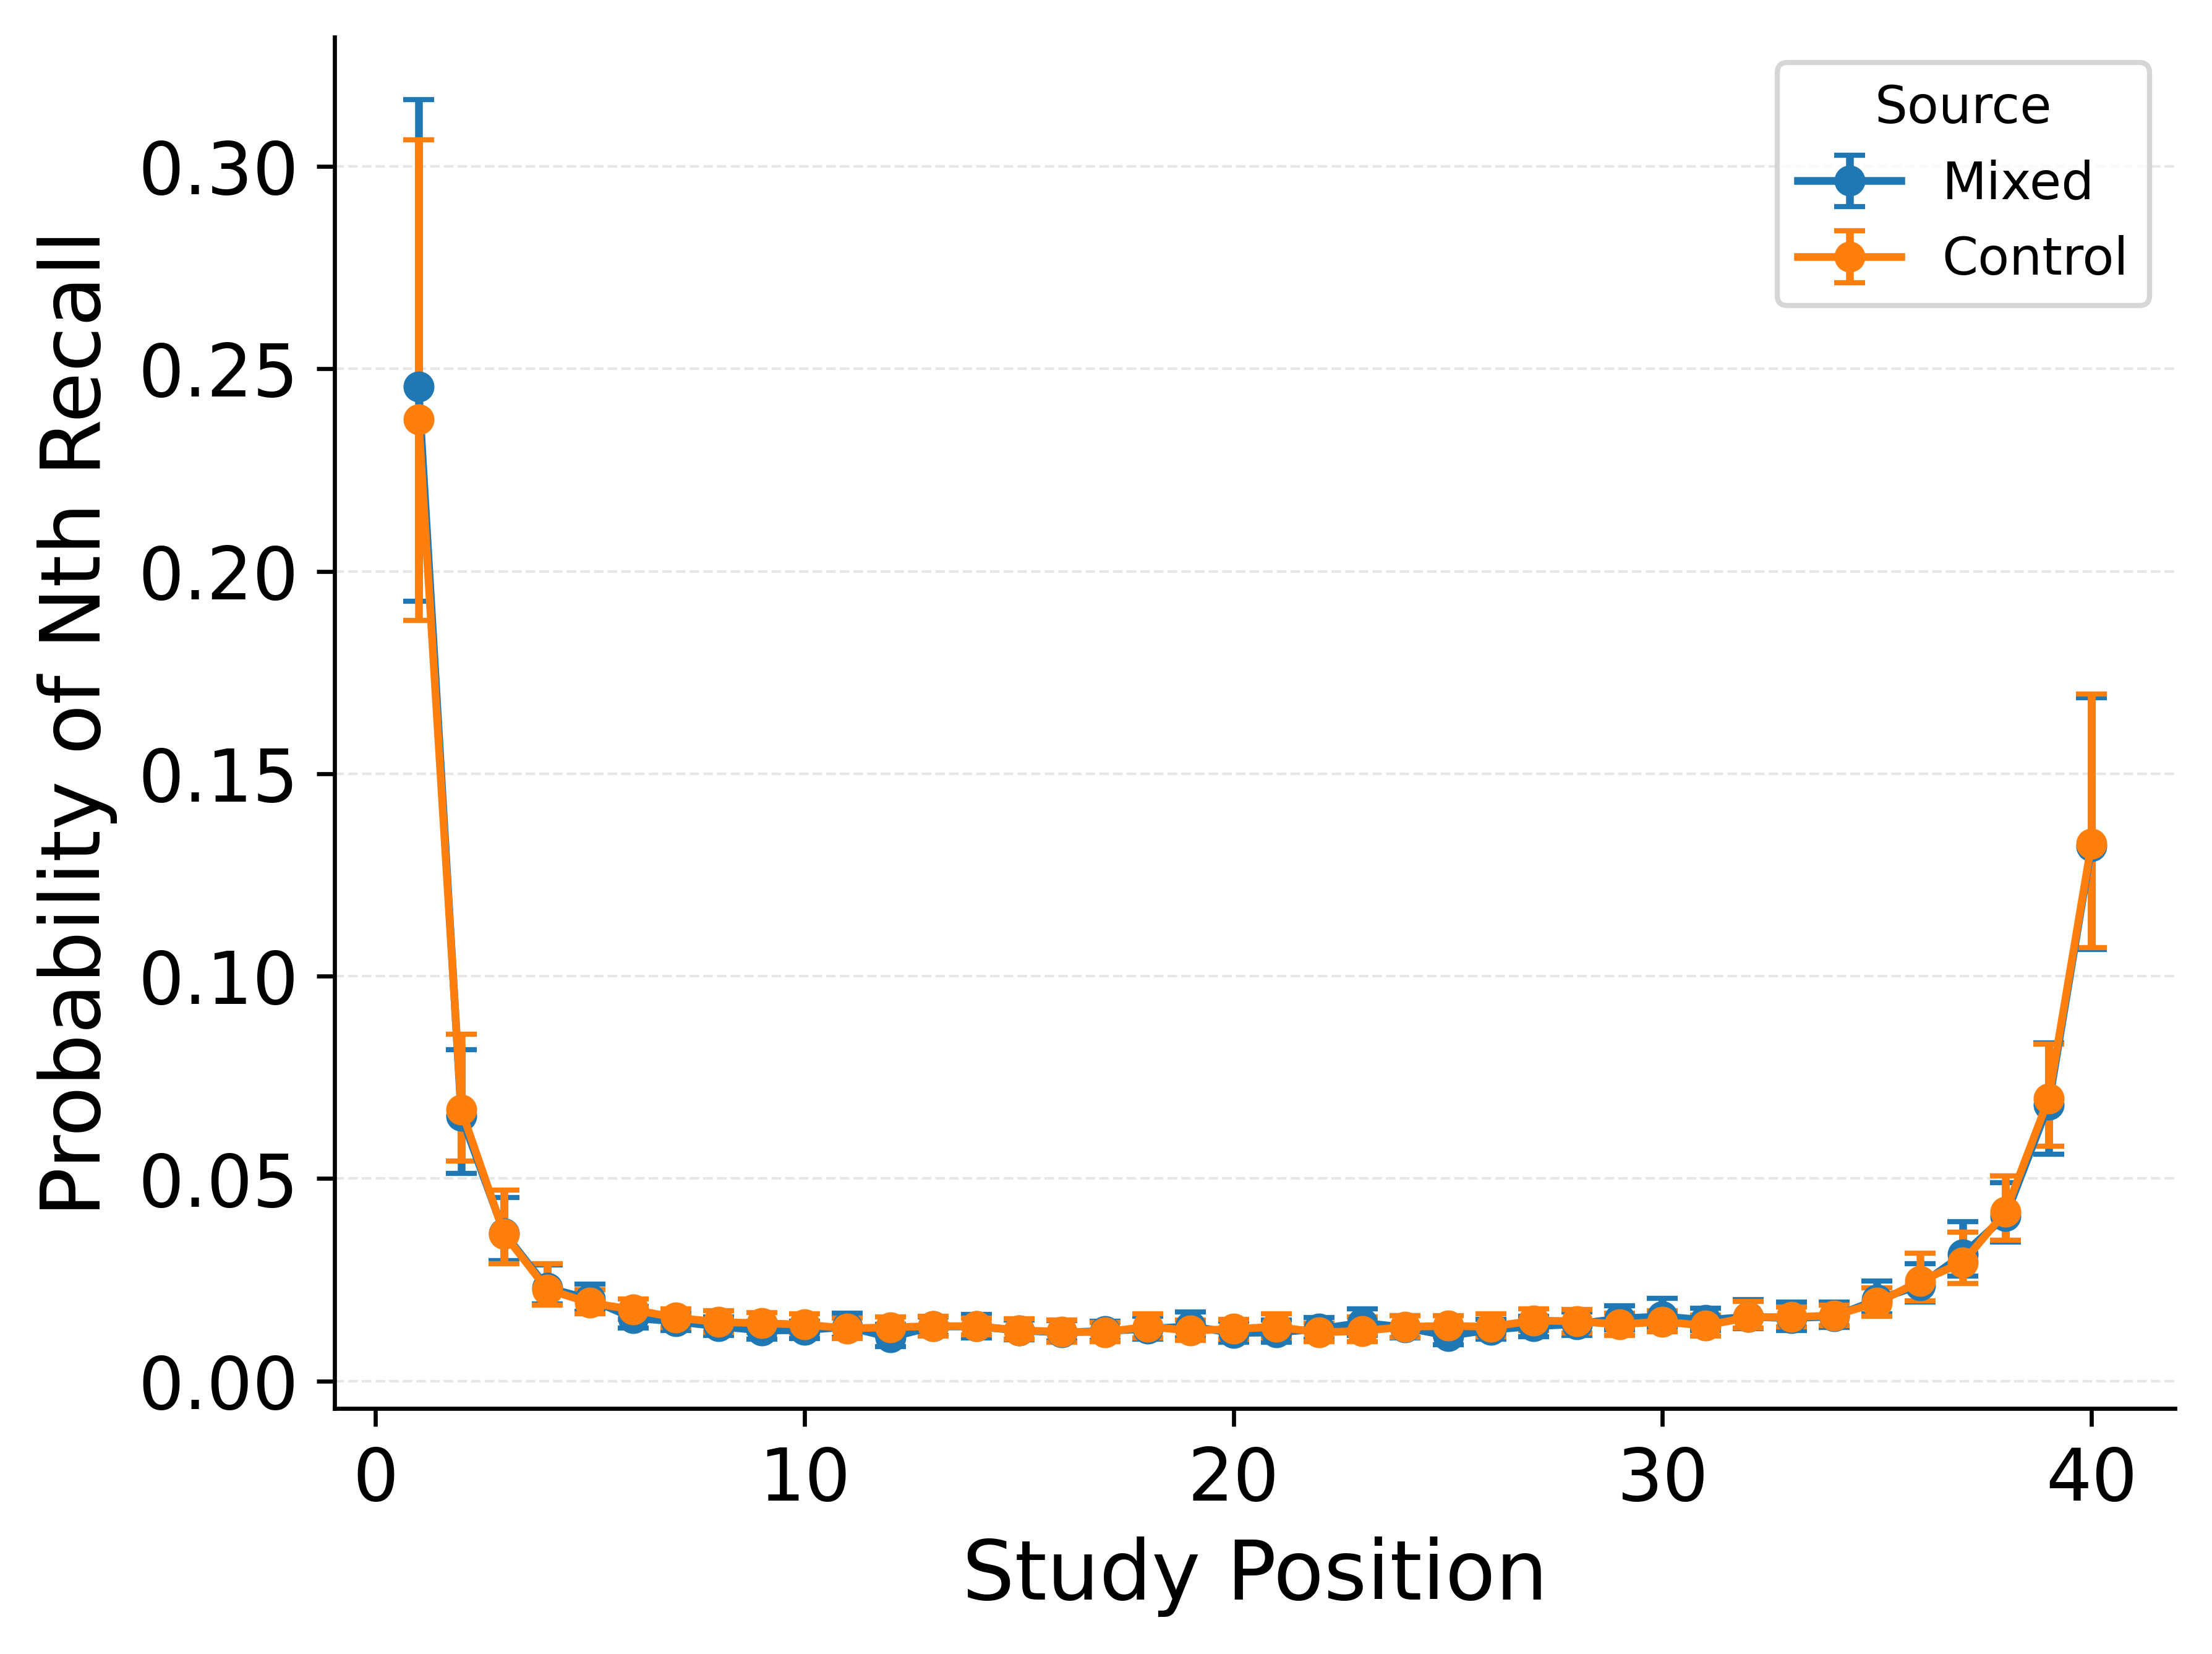
\includegraphics{../../work/thesis/figures/LohnasKahana2014_mixedvscontrolA_WeirdPositionalCMR_full_best_of_3_LT4_pnr.png}\end{minipage}%

\end{figure}%

Like standard CMR and CMR-NoSPR, Instance-CMR reproduces a robust,
monotonic spacing advantage (Figure~\ref{fig-icmr_os_spacing}). As
before, removing study-phase knitting and adding occurrence-specific
reinstatement does not blunt the spacing function, indicating that
contextual variability plus test-phase reinstatement suffices for this
benchmark in these paradigms.

\begin{figure}

\caption{\label{fig-icmr_os_spacing}\textbf{Instance-CMR spacing
function.} Simulated spacing curves for mixed vs matched-control lists
from Lohnas and Kahana (\citeproc{ref-lohnas2014retrieved}{2014}). The
spacing advantage is preserved without blending at test; the model does
not reproduce the apparent steeper slope for mixed lists in the data
(cf. Figure~\ref{fig-spacing}).}

\begin{minipage}{\linewidth}

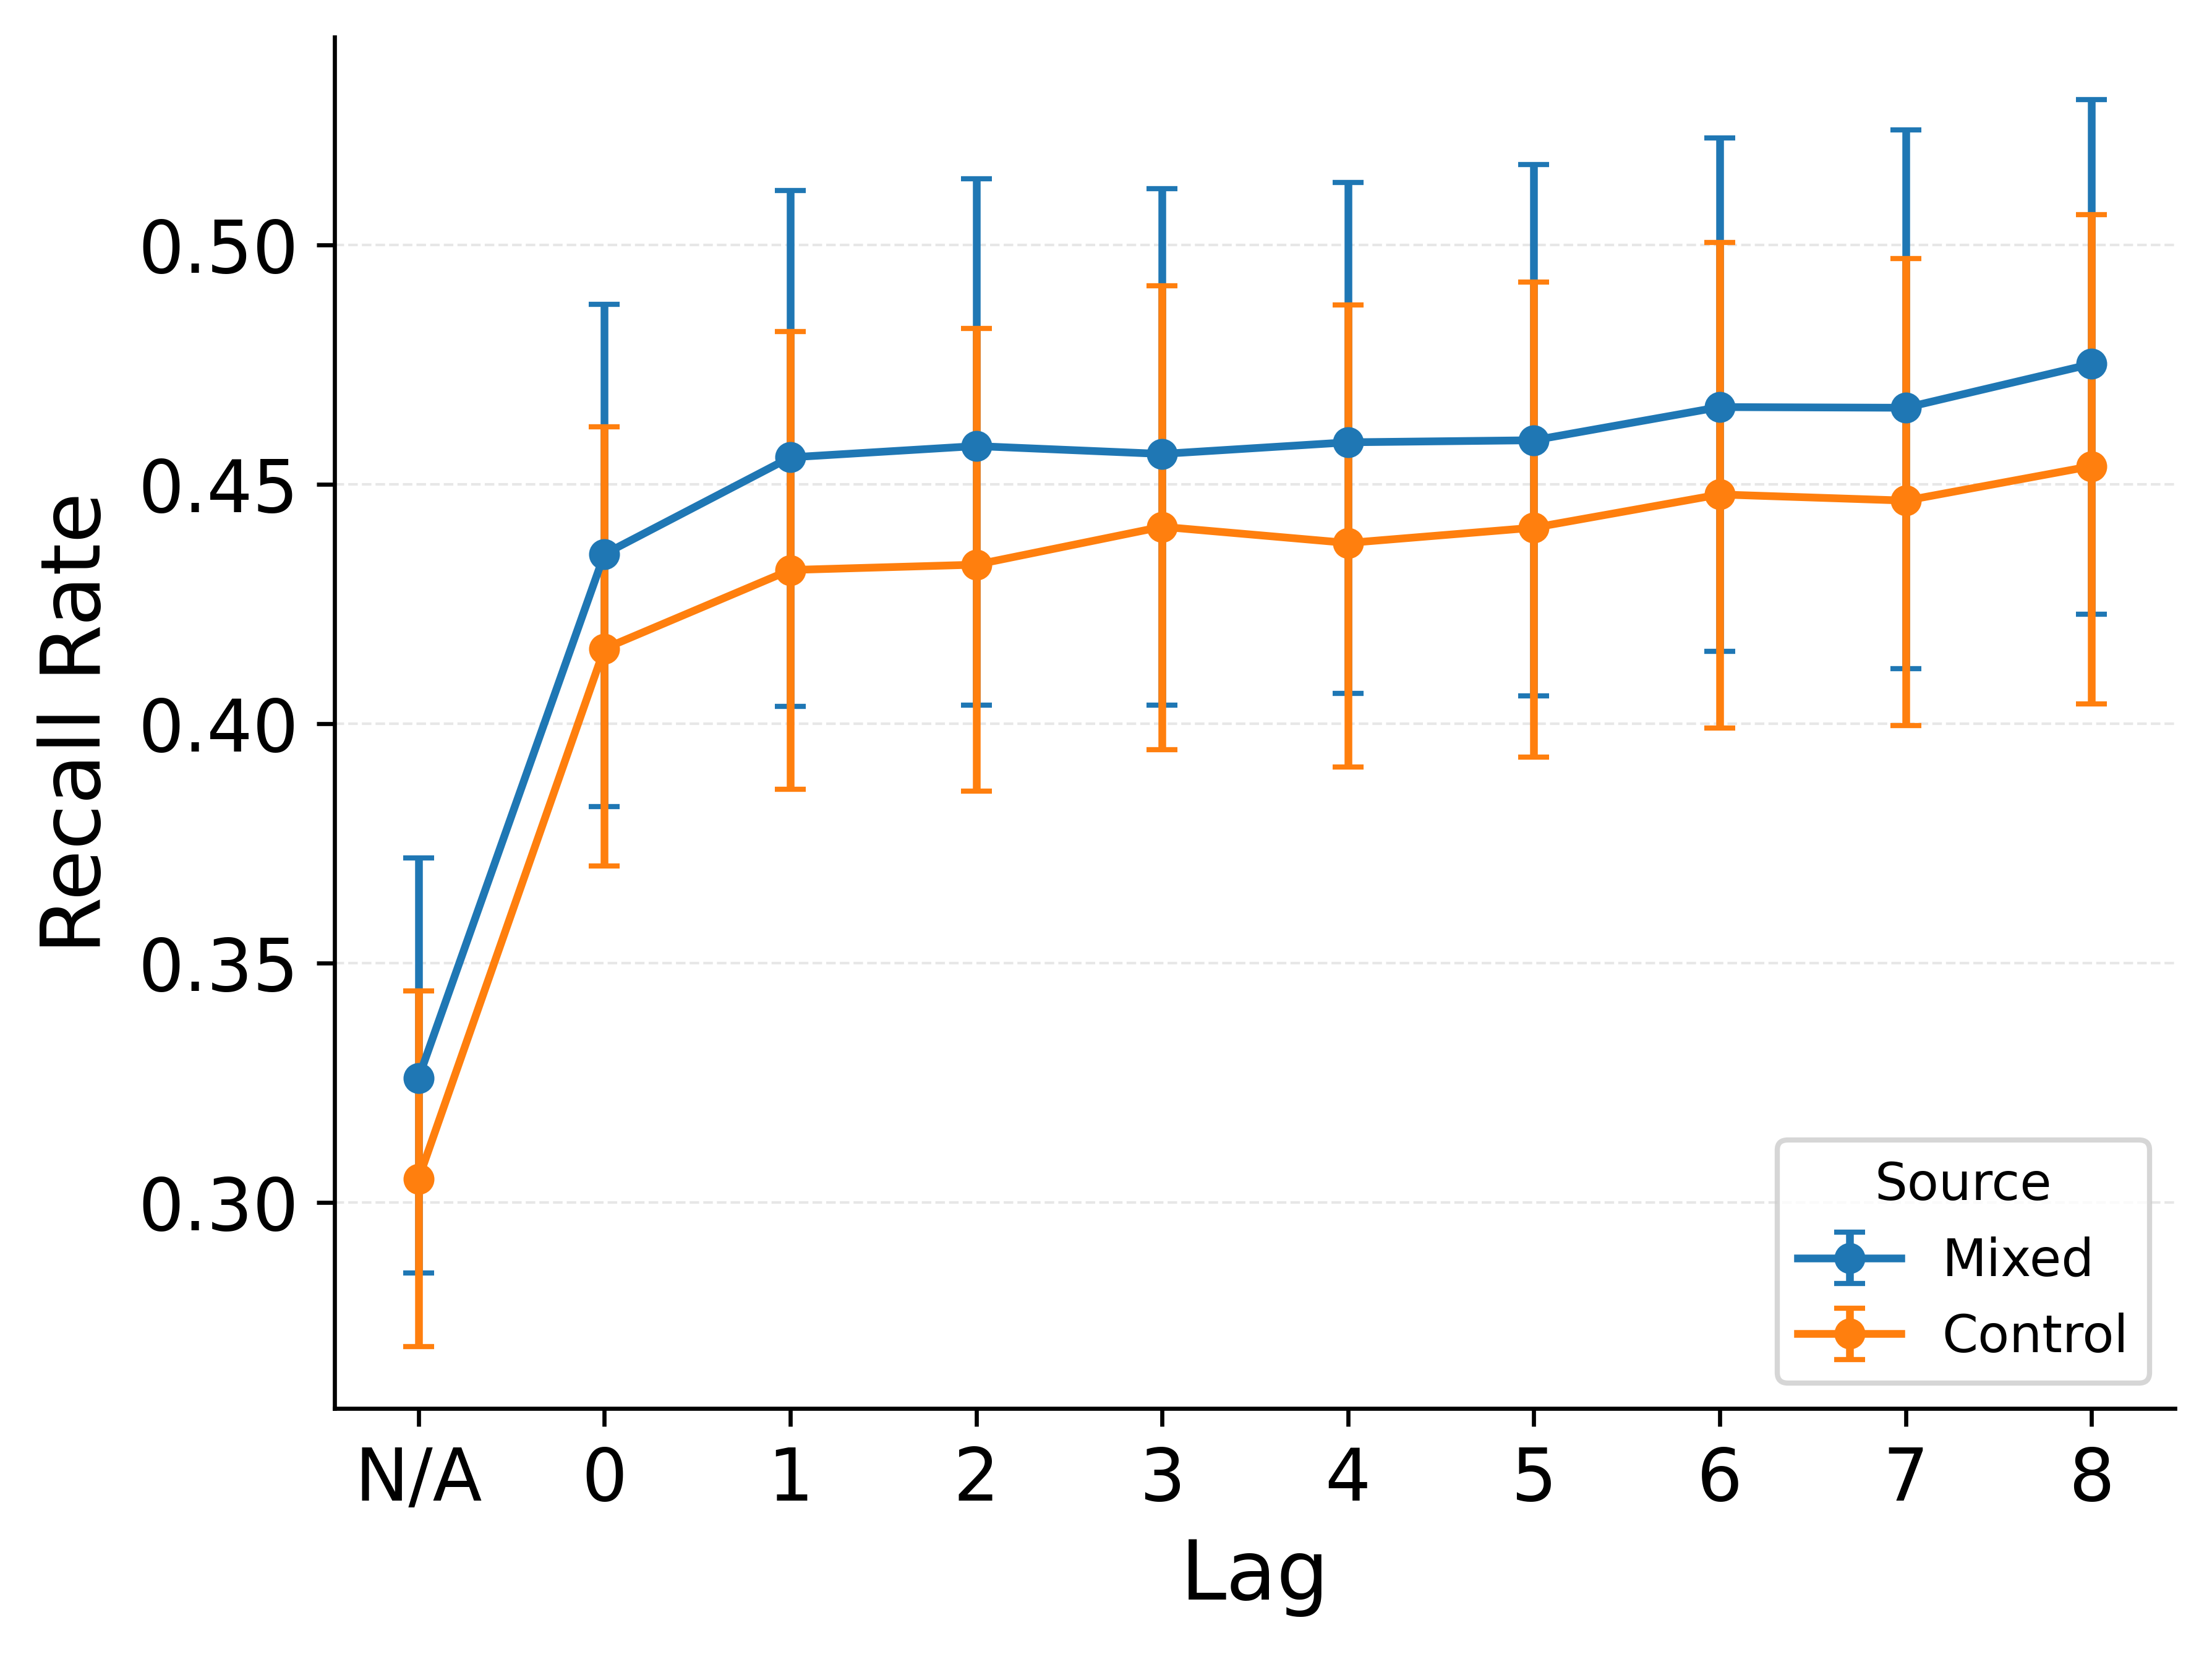
\includegraphics{../../work/thesis/figures/LohnasKahana2014_mixedvscontrolA_WeirdPositionalCMR_full_best_of_3_LT4_full_rpl.png}

\end{minipage}%

\end{figure}%

Next we consider cross-occurrence neighbor contiguity. Because
Instance-CMR keeps occurrence contexts distinct at study (as in
CMR-NoSPR) and selective at test (no blending when the repeater is later
recalled), the model predicts no elevation of cross-occurrence neighbor
transitions. In the centered neighbor-contiguity tests,
mixed--minus--baseline curves remain near zero in both directions
(Figure~Figure~\ref{fig-os_neighbor_contiguity}), matching the data's
non-elevation and improving on standard CMR's incorrect peaks.

\begin{figure}

\caption{\label{fig-os_neighbor_contiguity}Instance-CMR:
cross-occurrence neighbor transitions (centered lag-CRPs). Left:
triggers from forward neighbors of the \emph{first} presentation
(\(i{+}1,i{+}2\)), lags centered on the \emph{second}
(\(\ell=\text{next}-j\)). Right: symmetric variant (triggers
\(j{+}1,j{+}2\); lags centered on \(i\)). Mixed--minus--baseline curves
sit at baseline in both directions, consistent with no knitting across
neighborhoods.}

\begin{minipage}{0.50\linewidth}
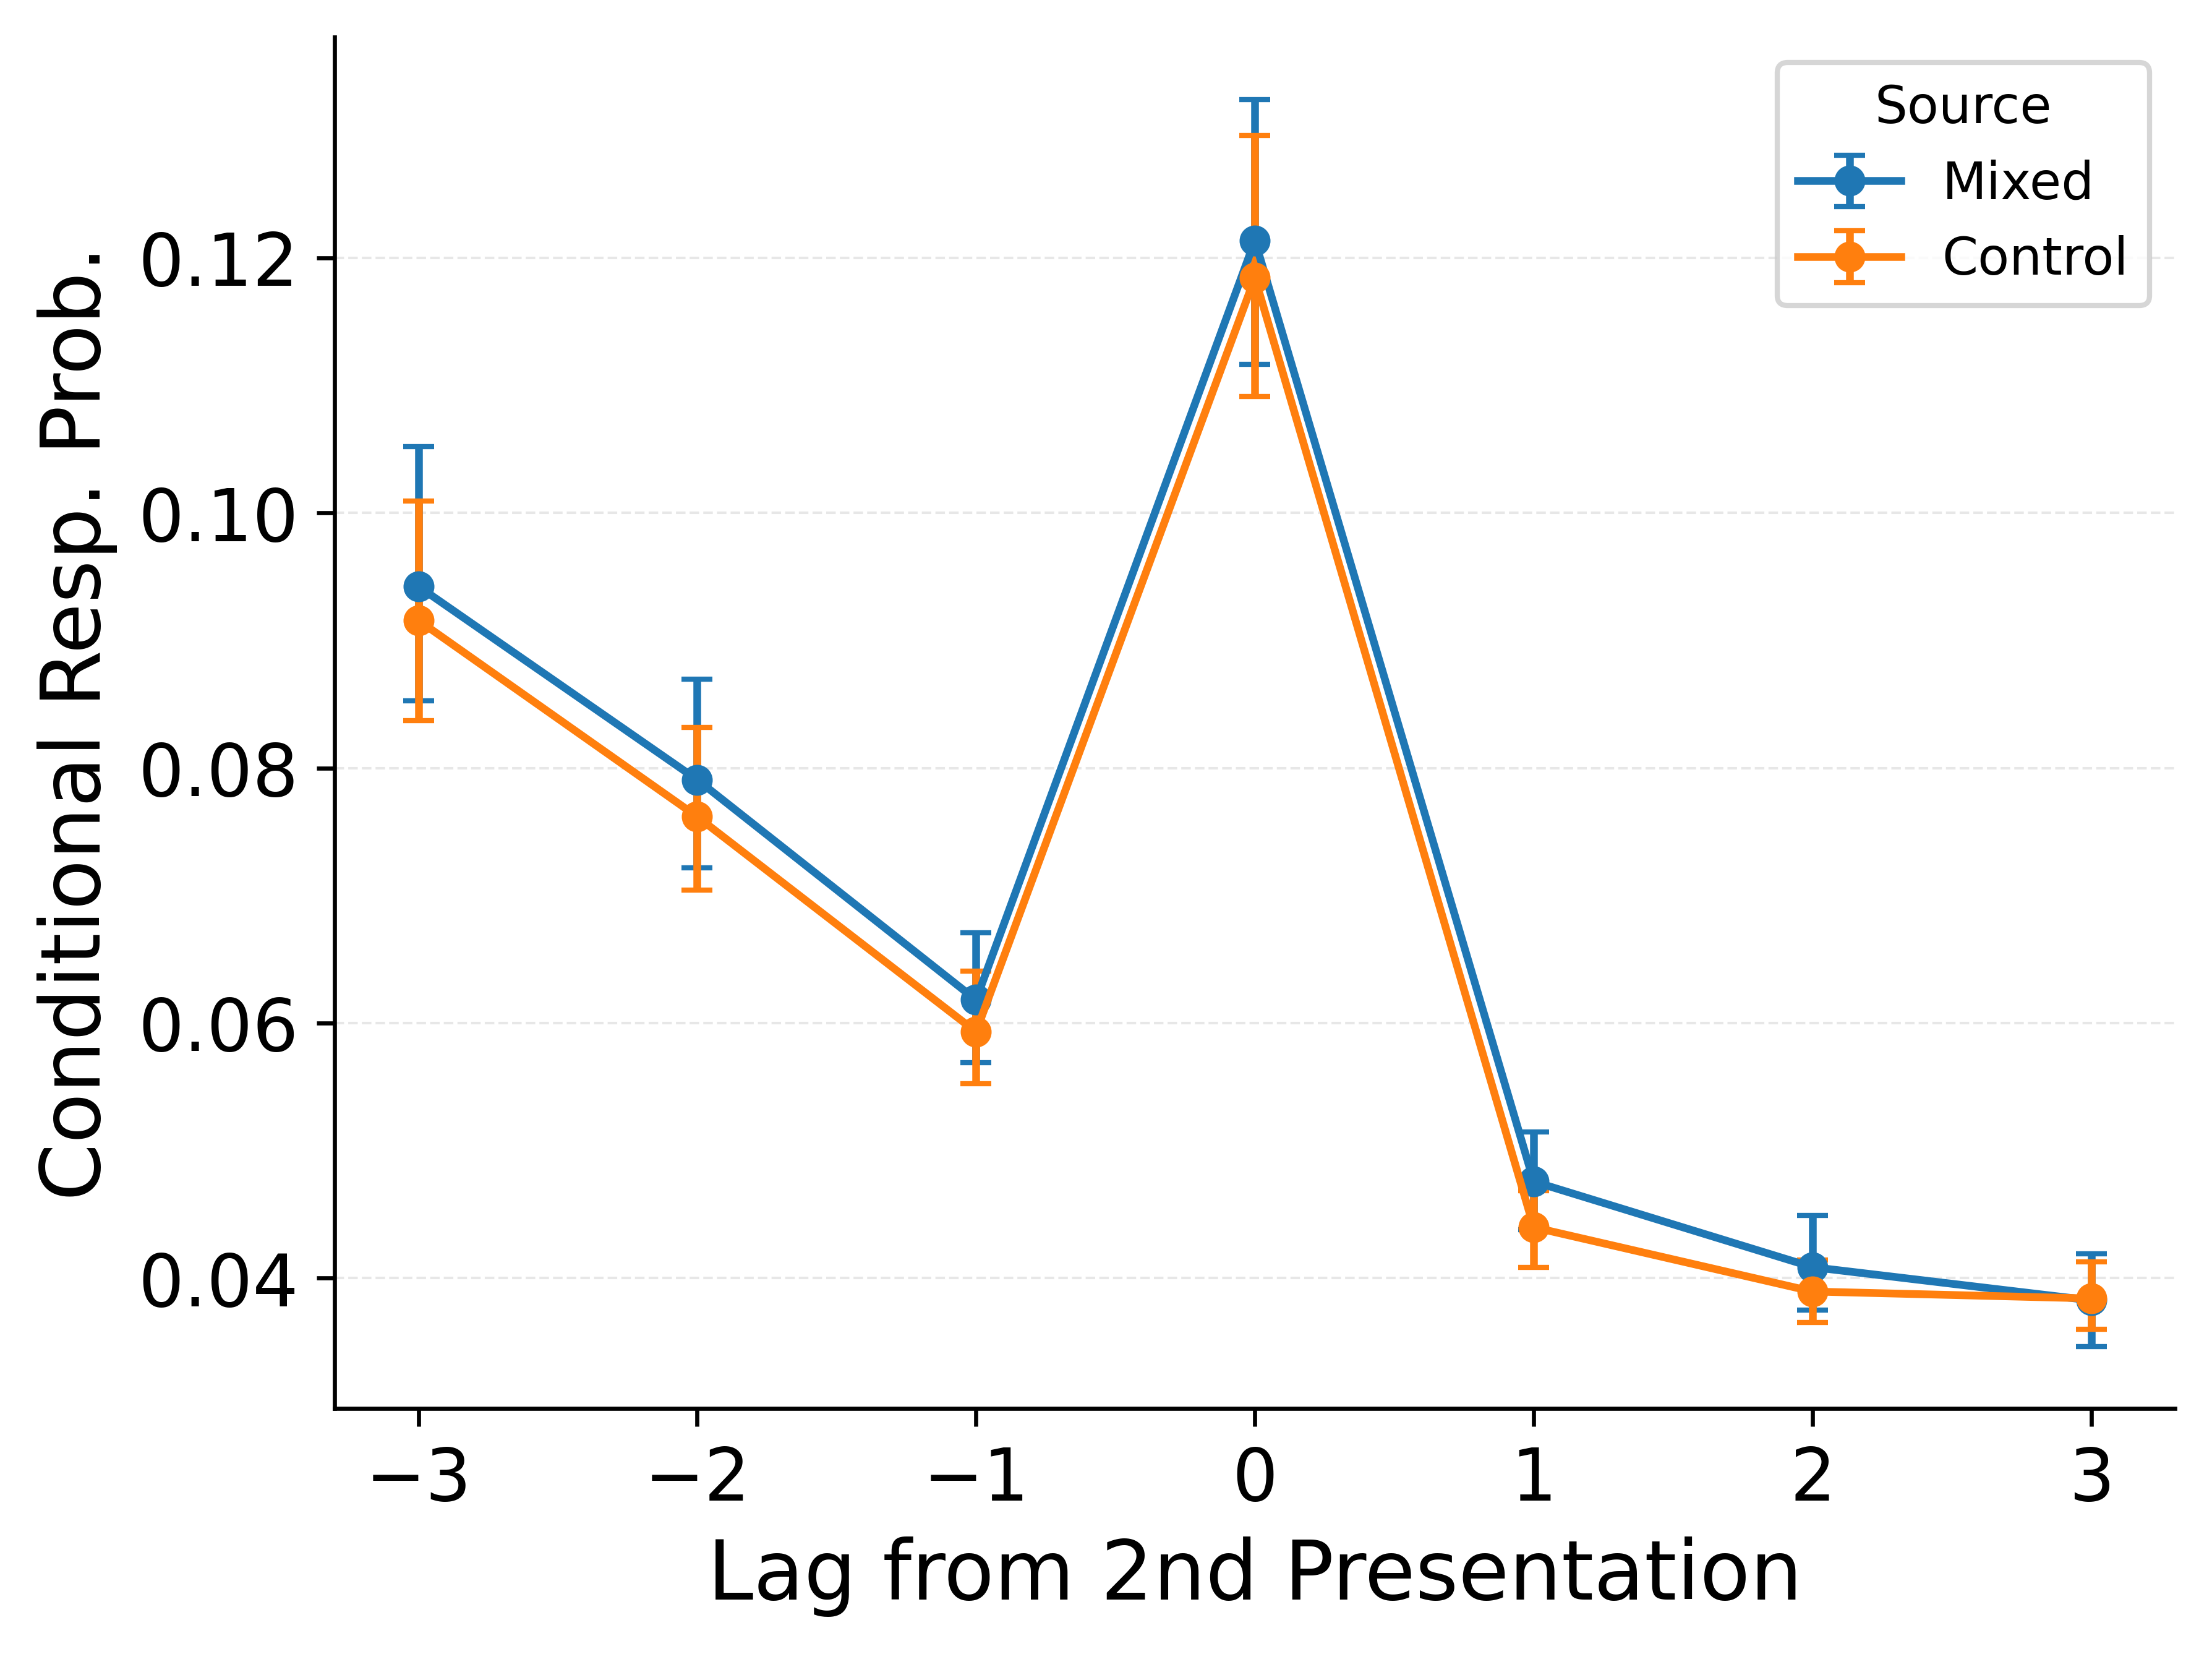
\includegraphics{../../work/thesis/figures/LohnasKahana2014_mixedvscontrolA_WeirdPositionalCMR_full_best_of_3_LT4_repneighborcrp_i2j.png}\end{minipage}%
%
\begin{minipage}{0.50\linewidth}
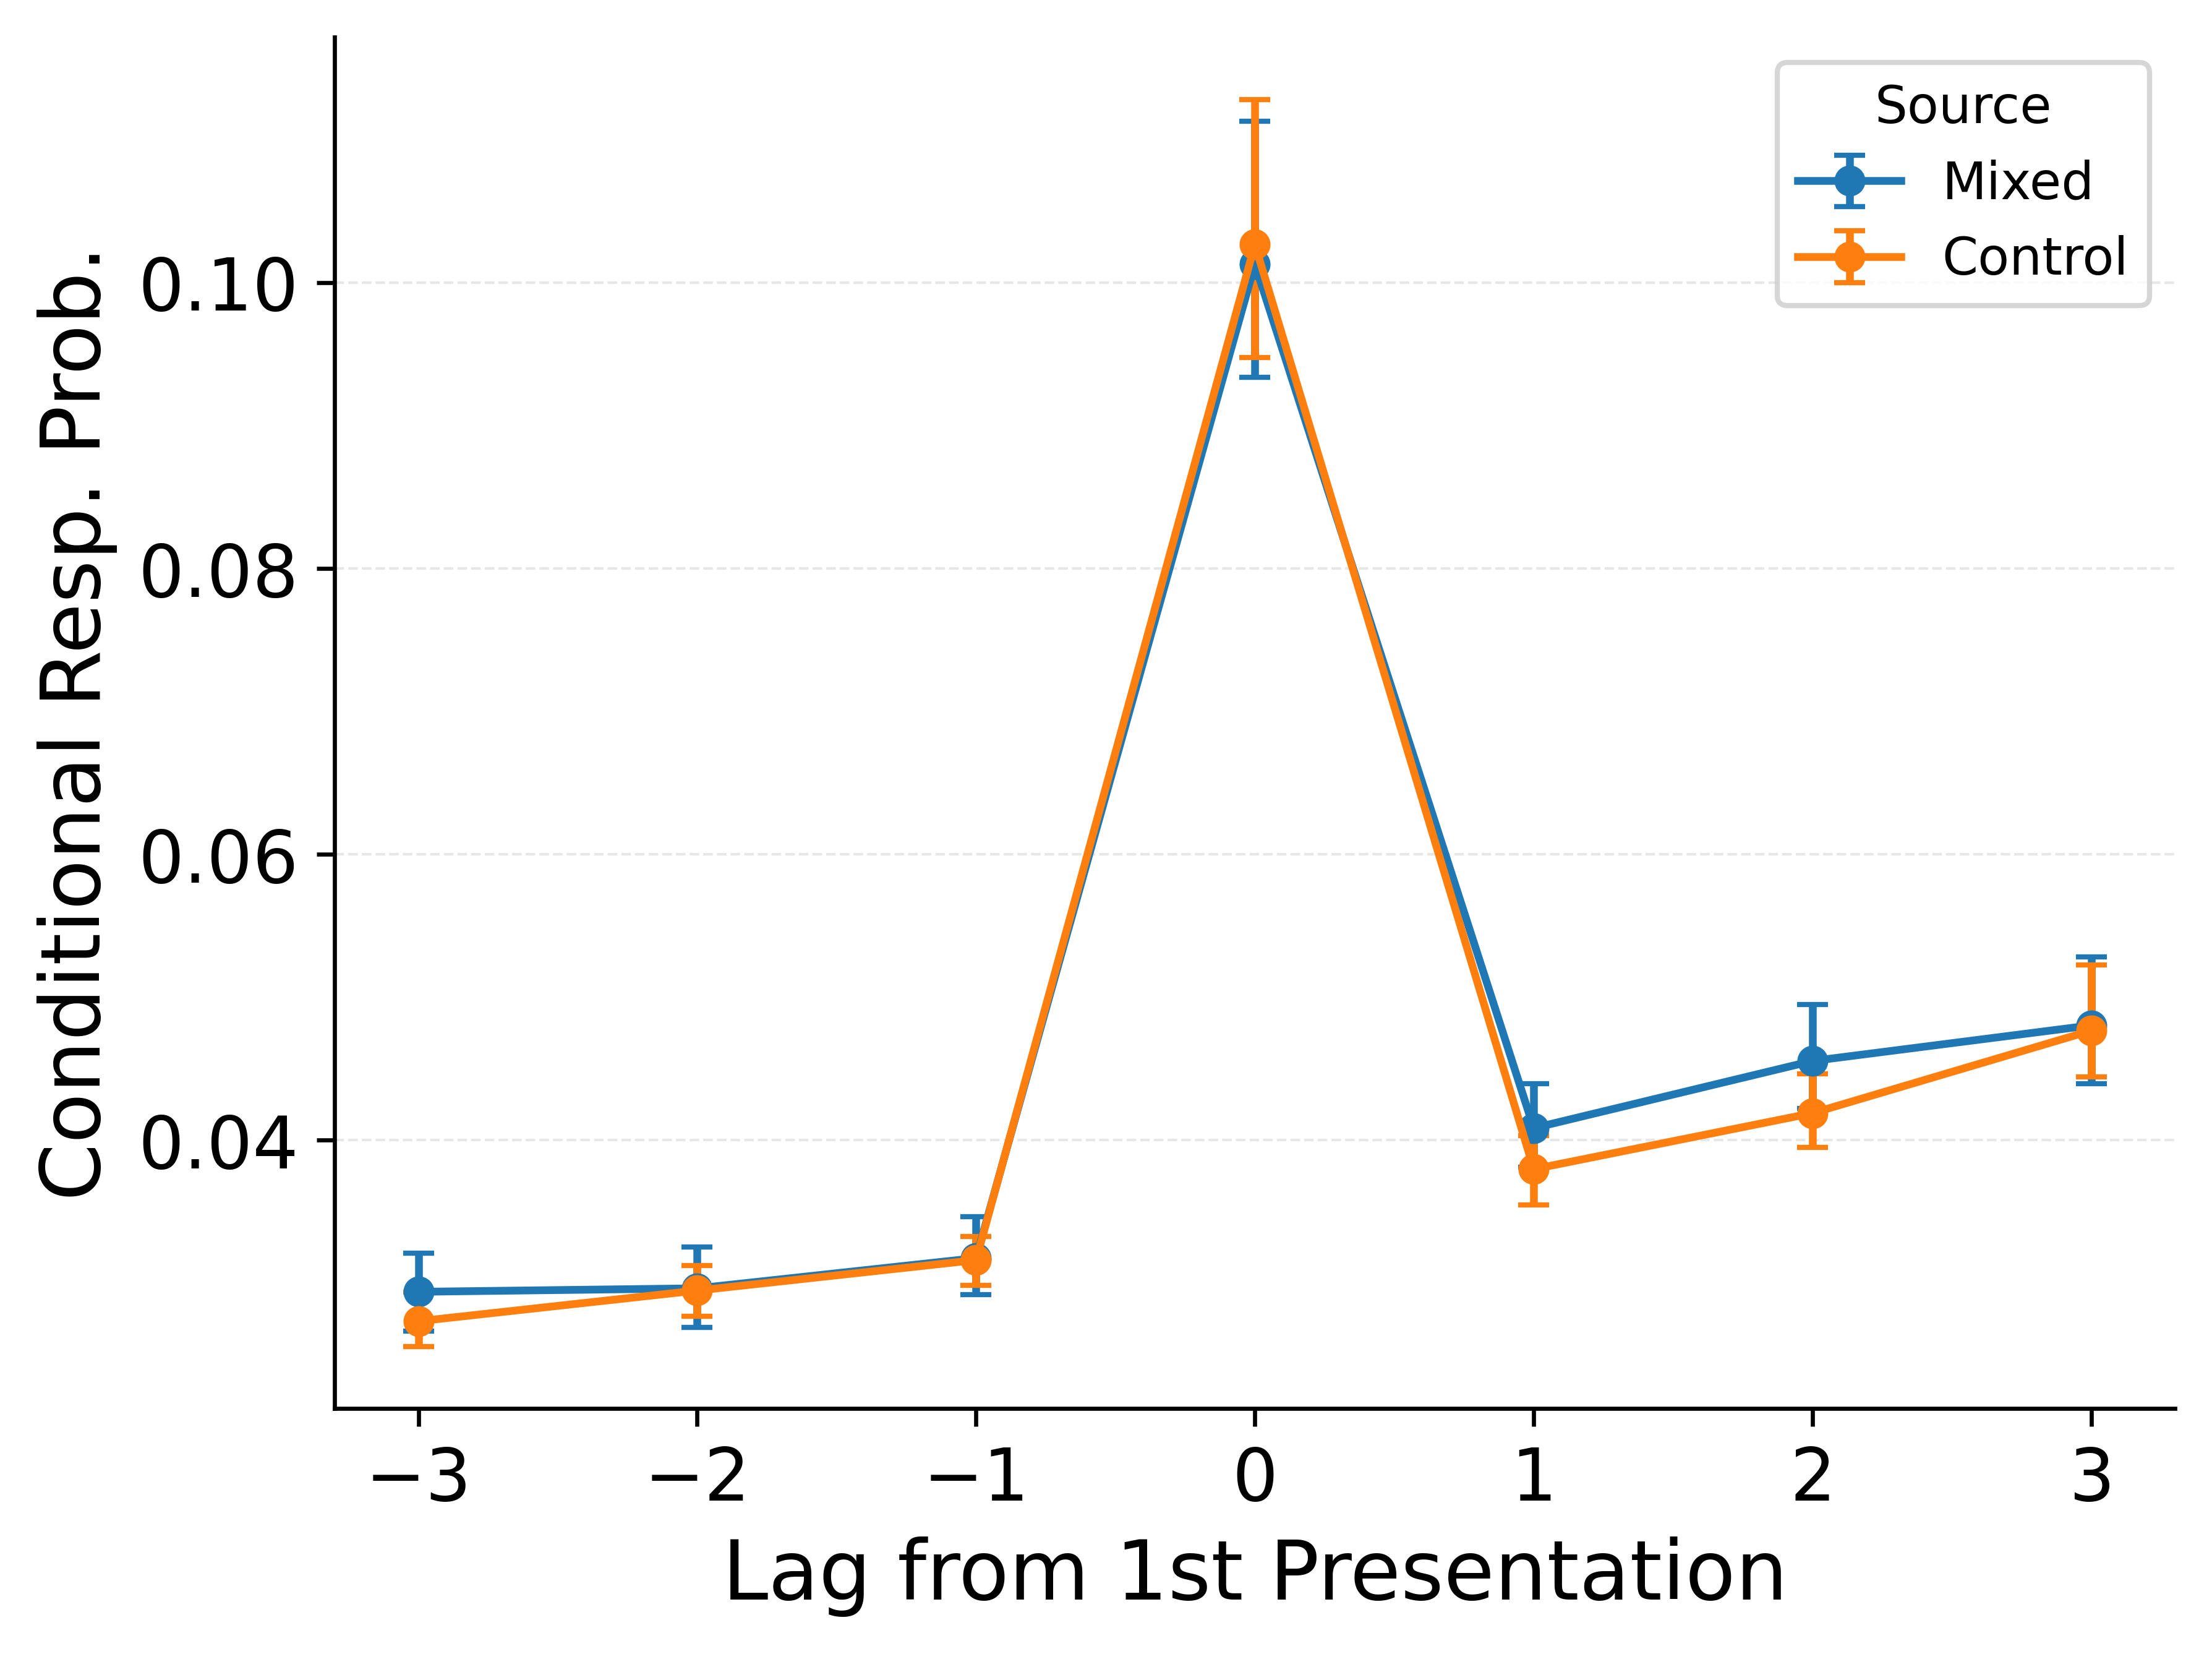
\includegraphics{../../work/thesis/figures/LohnasKahana2014_mixedvscontrolA_WeirdPositionalCMR_full_best_of_3_LT4_repneighborcrp_j2i.png}\end{minipage}%

\end{figure}%

Next we consider the outgoing Repetition Lag-CRP where the critical
change appears when the repeater itself is recalled. By routing
reinstatement through a single occurrence, Instance-CMR removes the
balanced-access signature that arises from blending in standard CMR and
persists in CMR-NoSPR. Consequently, the model preserves the
first-over-second preference seen in controls rather than washing it out
(Figure~\ref{fig-os_rep_lag_crp}). However, Instance-CMR does not
generate the extra first-over-second separation evident in the data's
mixed-minus-baseline contrast; the model's separation is essentially
equal to baseline, not boosted. This resolves the
associative-interference prediction but leaves a positive,
repetition-specific asymmetry unexplained.

In the incoming/backward Repetition Lag-CRP (not displayed), selective
reinstatement at test does little to the incoming variant, which
reflects how the search state approached the repeater. Instance-CMR
therefore predicts a modest first-over-second preference on arrivals,
comparable to CMR-NoSPR and still weaker than in the data. This
reinforces our earlier conclusion that the outgoing
mixed--minus--baseline contrast is the cleaner probe of
repetition-specific reinstatement.

\begin{figure}

\caption{\label{fig-os_rep_lag_crp}\textbf{Repetition lag-CRP
(outgoing): data vs Instance-CMR.} Top row: mixed lists (left) and
matched-control baseline (right) from Lohnas and Kahana
(\citeproc{ref-lohnas2014retrieved}{2014}). Bottom row: Instance-CMR
simulations scored identically. First- vs second-centered curves remain
separated (no blending). Unlike the data (top-left), the
mixed-minus-baseline separation is not substantially enlarged in
Instance-CMR, fixing interference but not the boosted first-over-second
advantage.}

\begin{minipage}{0.50\linewidth}
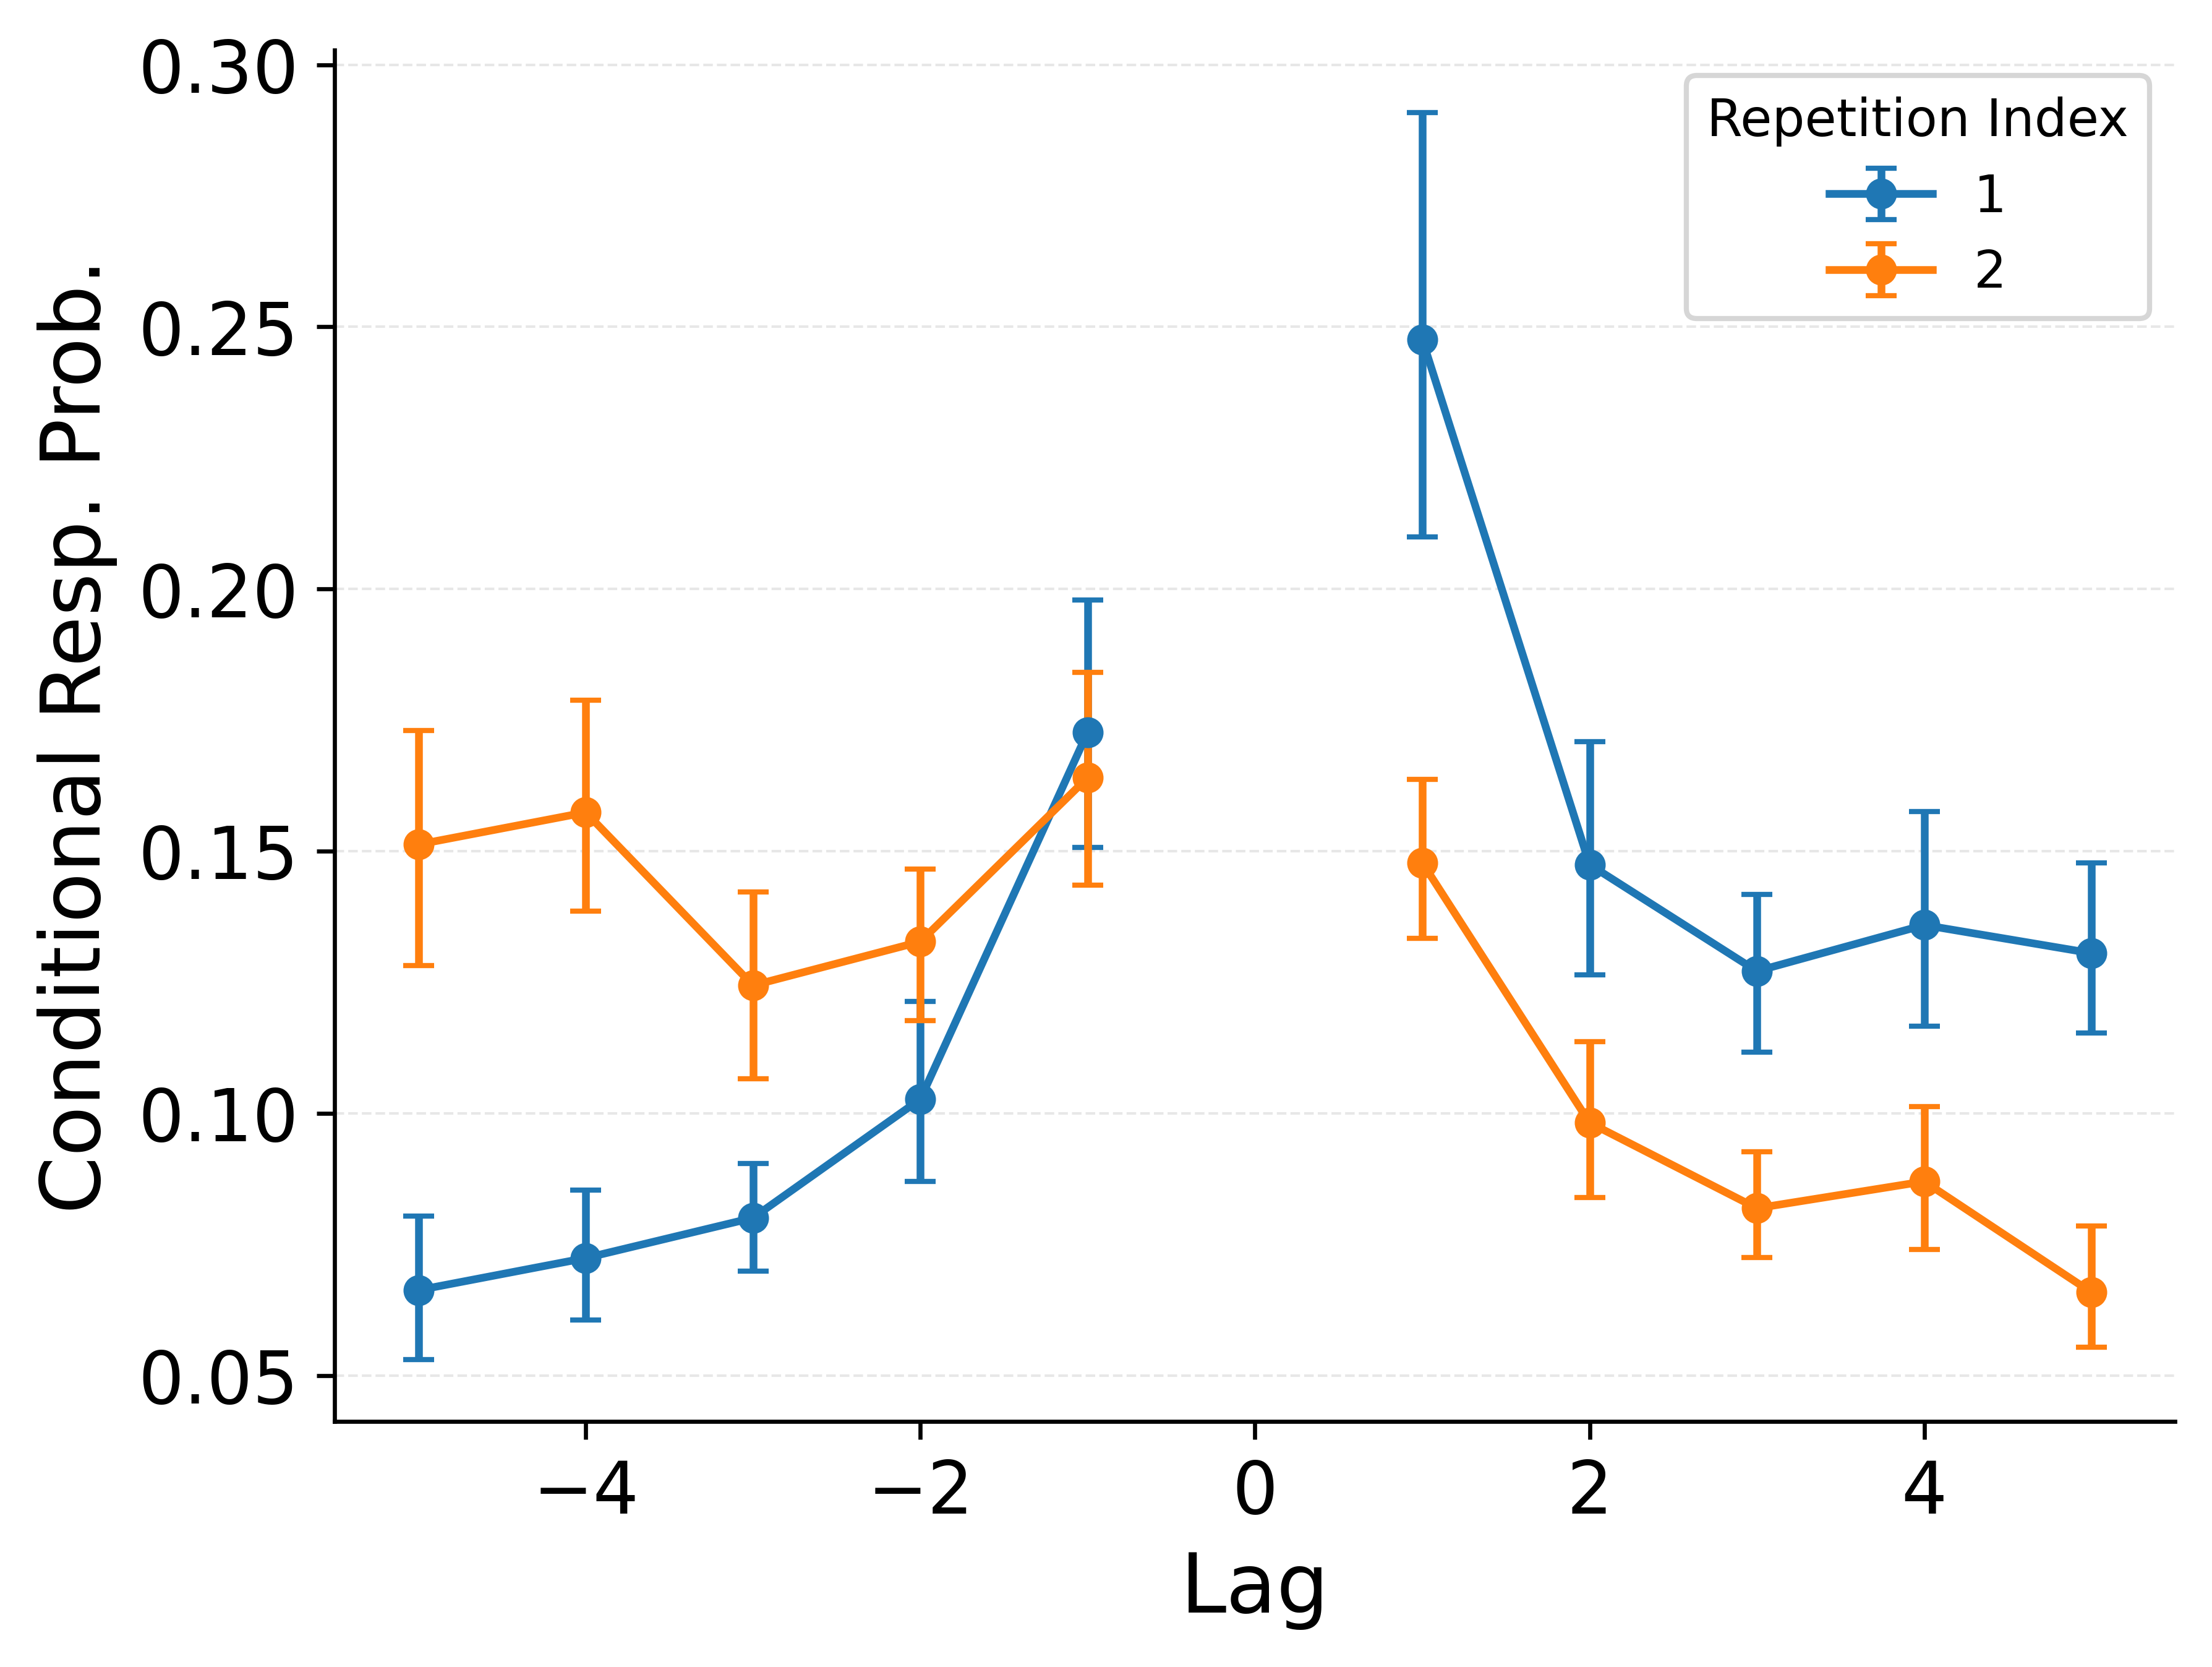
\includegraphics{../../work/thesis/figures/RepeatedRecallsLohnasKahana2014_mixed_data_full_best_of_3_LT34_rep_crp.png}\end{minipage}%
%
\begin{minipage}{0.50\linewidth}
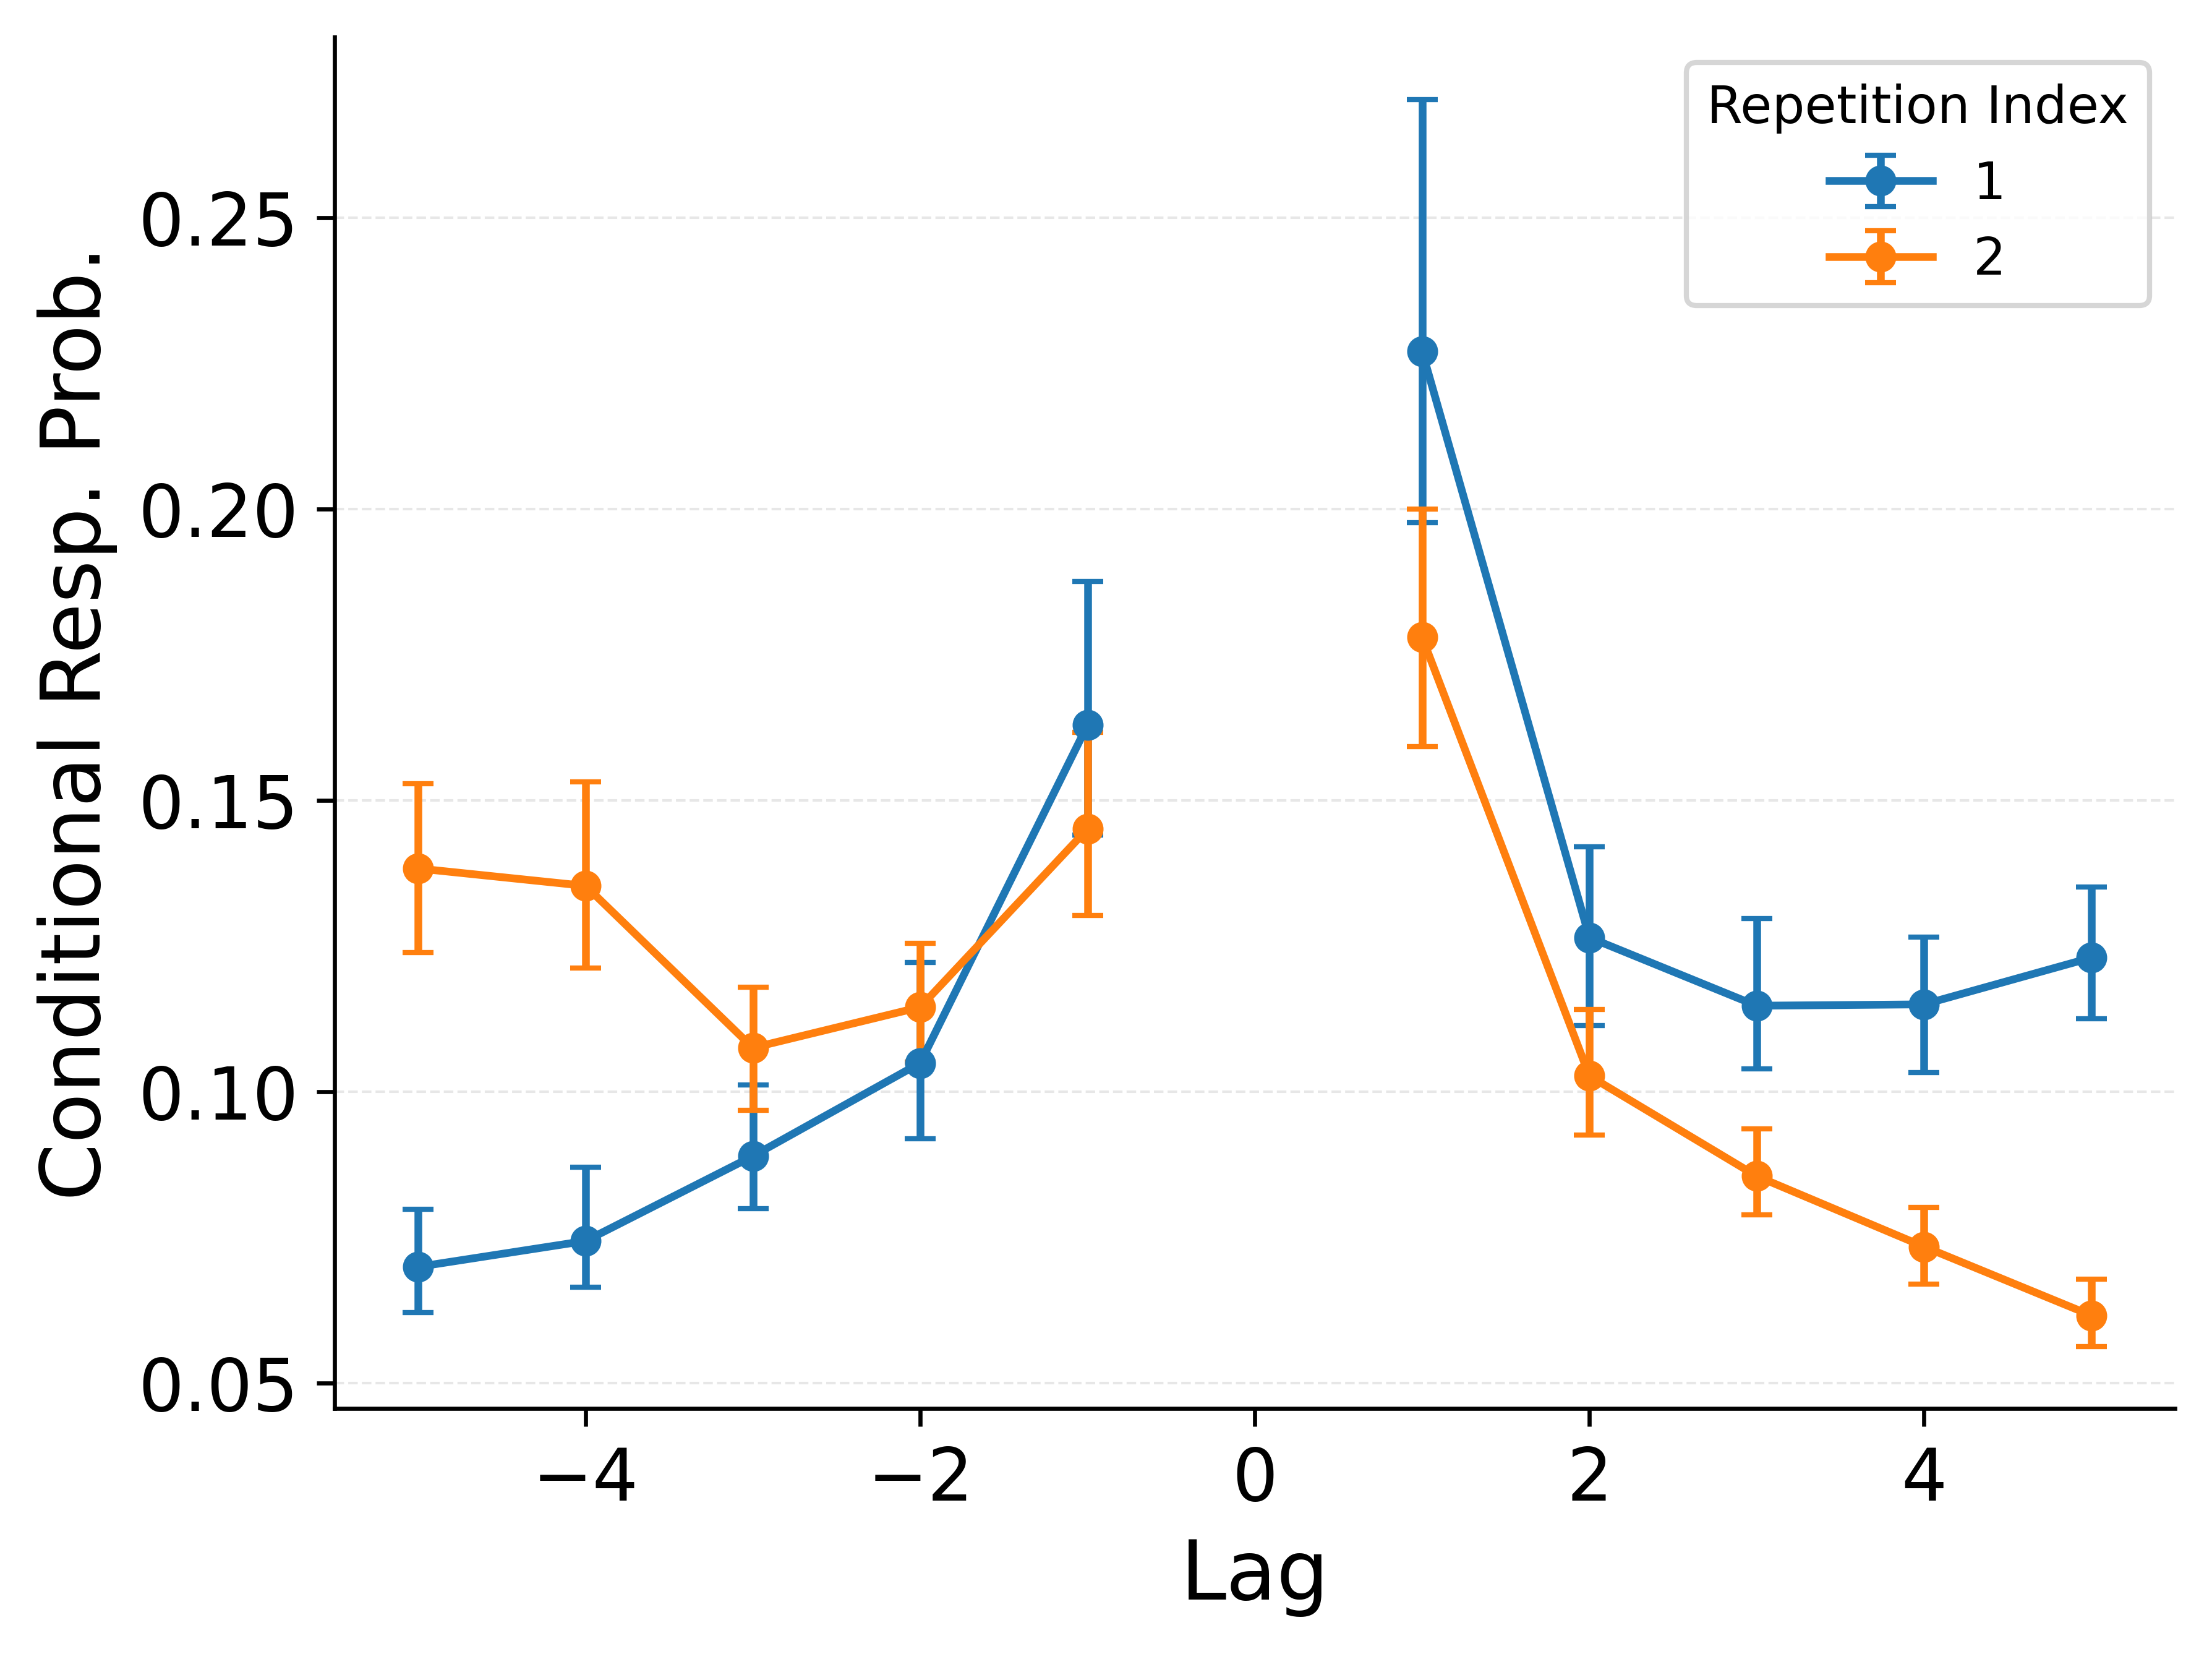
\includegraphics{../../work/thesis/figures/RepeatedRecallsLohnasKahana2014_control_data_full_best_of_3_LT34_rep_crp.png}\end{minipage}%
\newline
\begin{minipage}{0.50\linewidth}
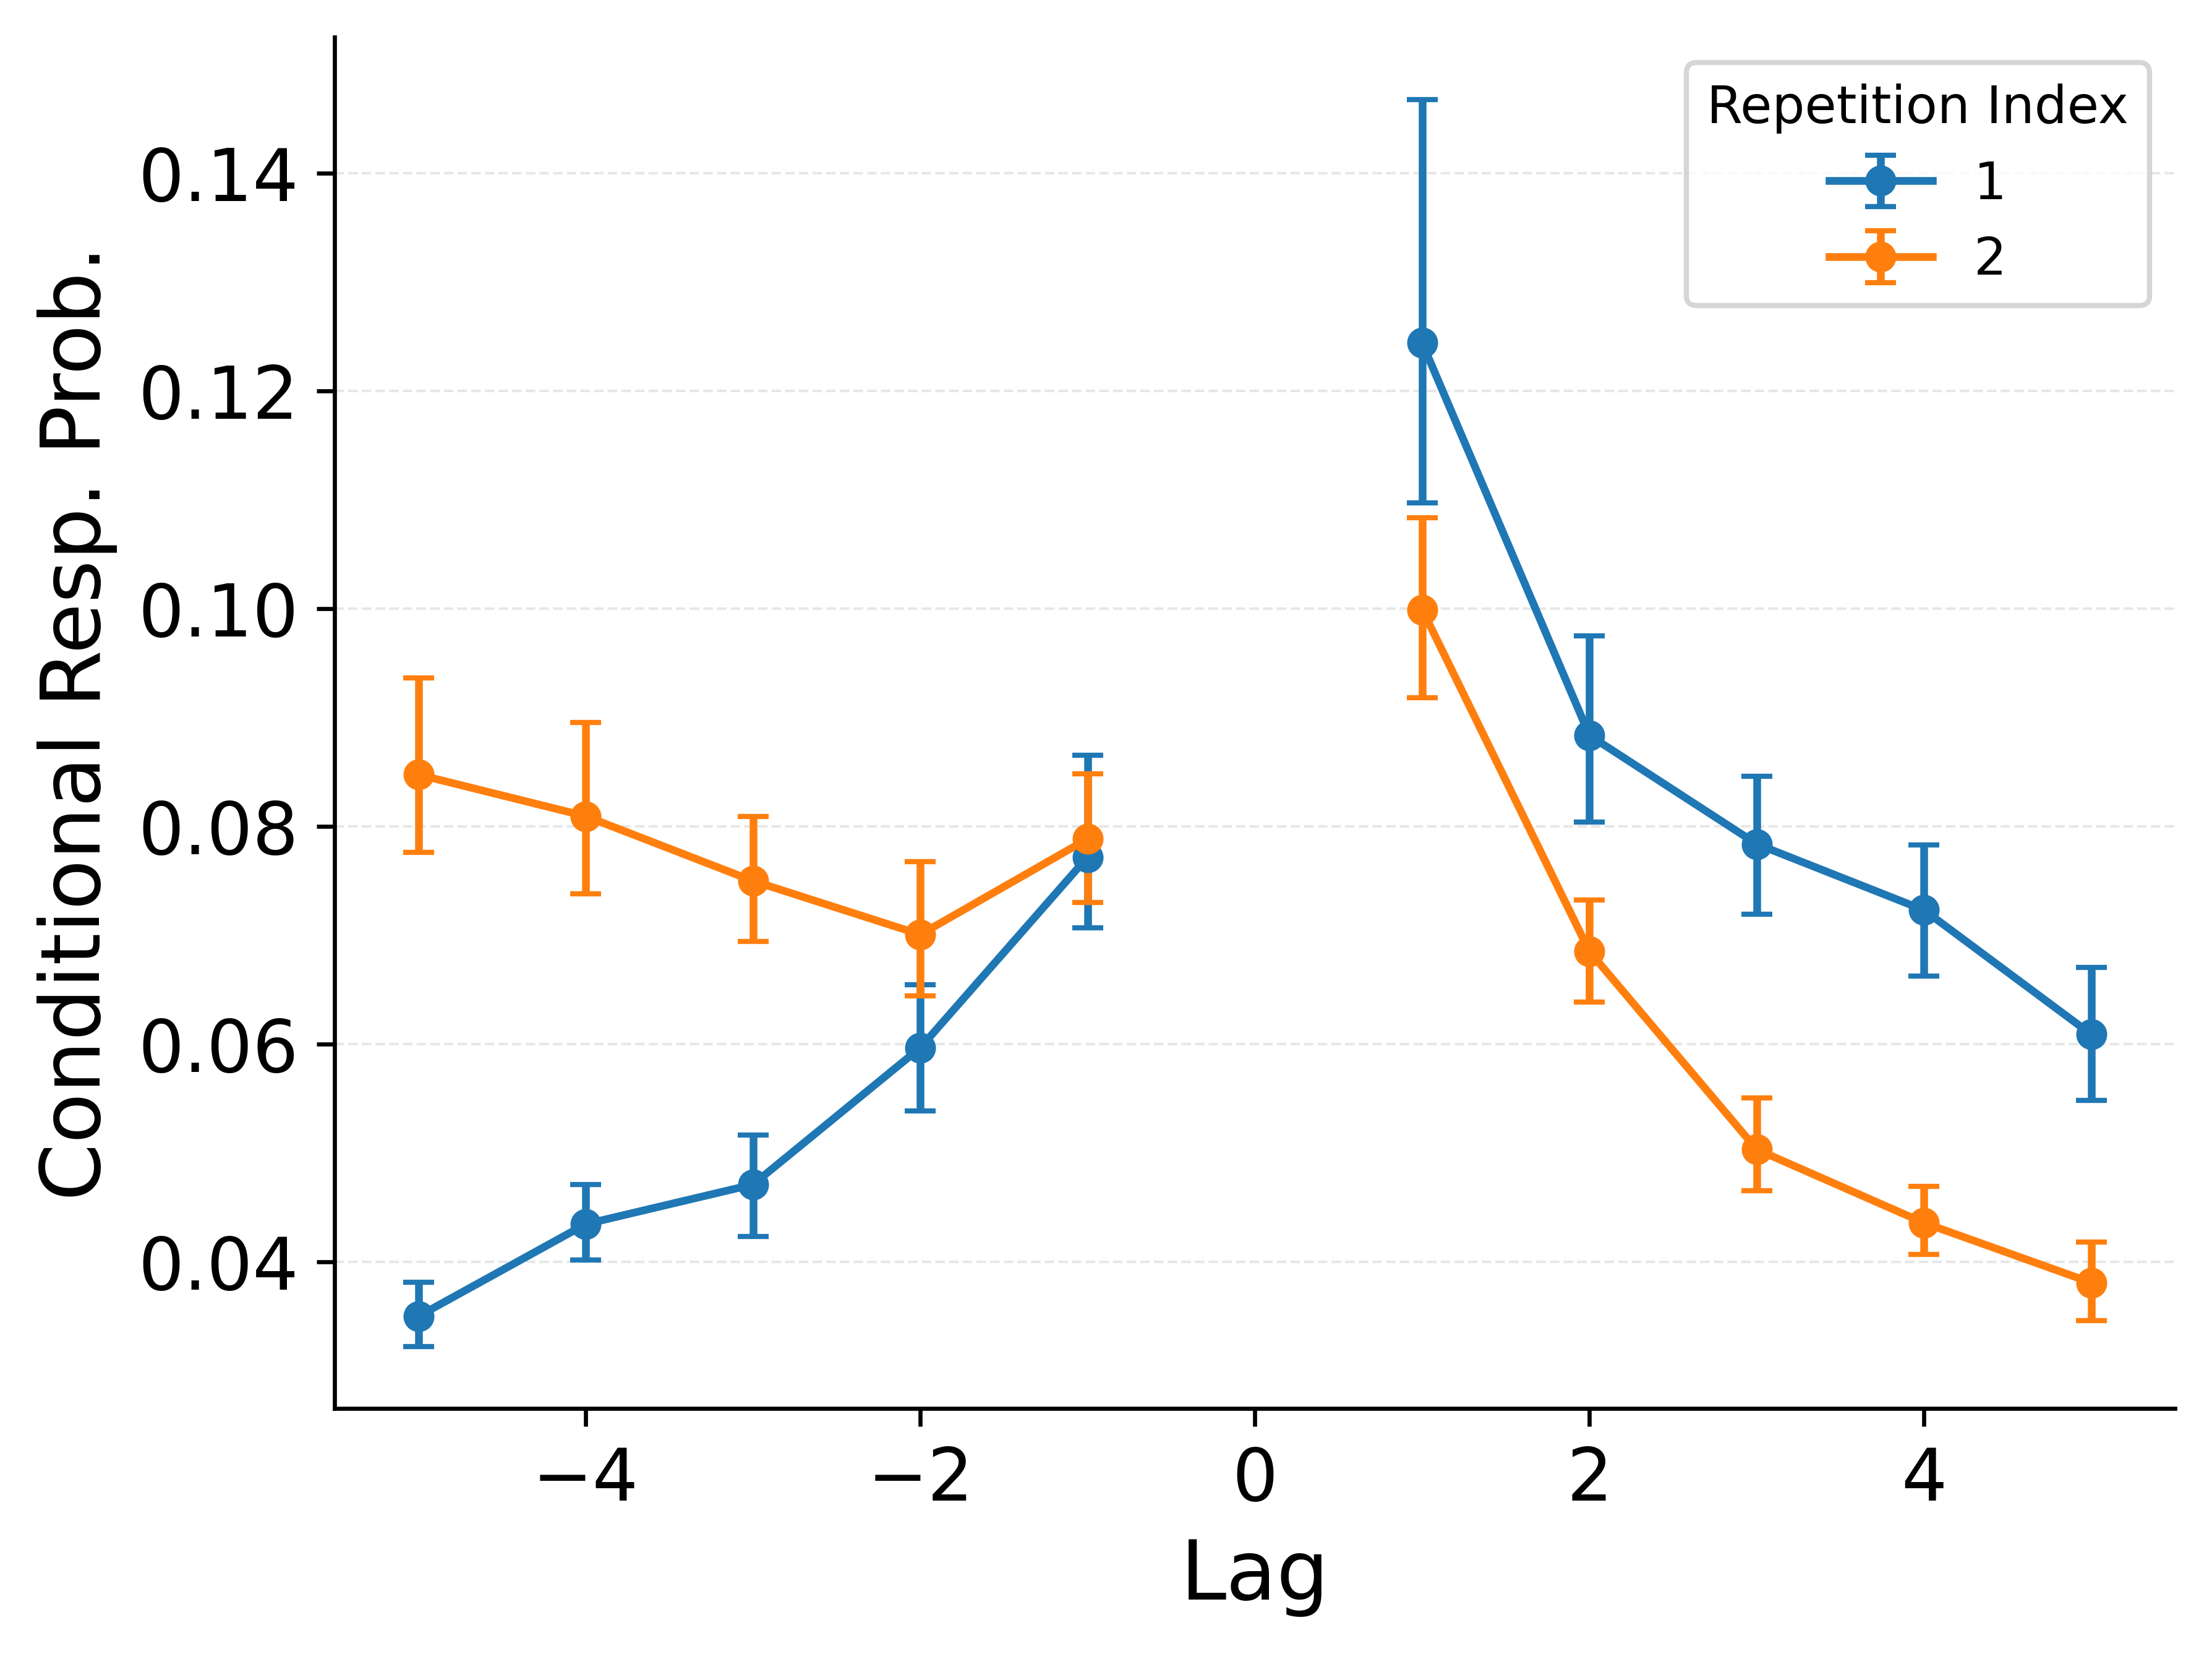
\includegraphics{../../work/thesis/figures/LohnasKahana2014_mixed_WeirdPositionalCMR_full_best_of_3_LT4_rep_crp.png}\end{minipage}%
%
\begin{minipage}{0.50\linewidth}
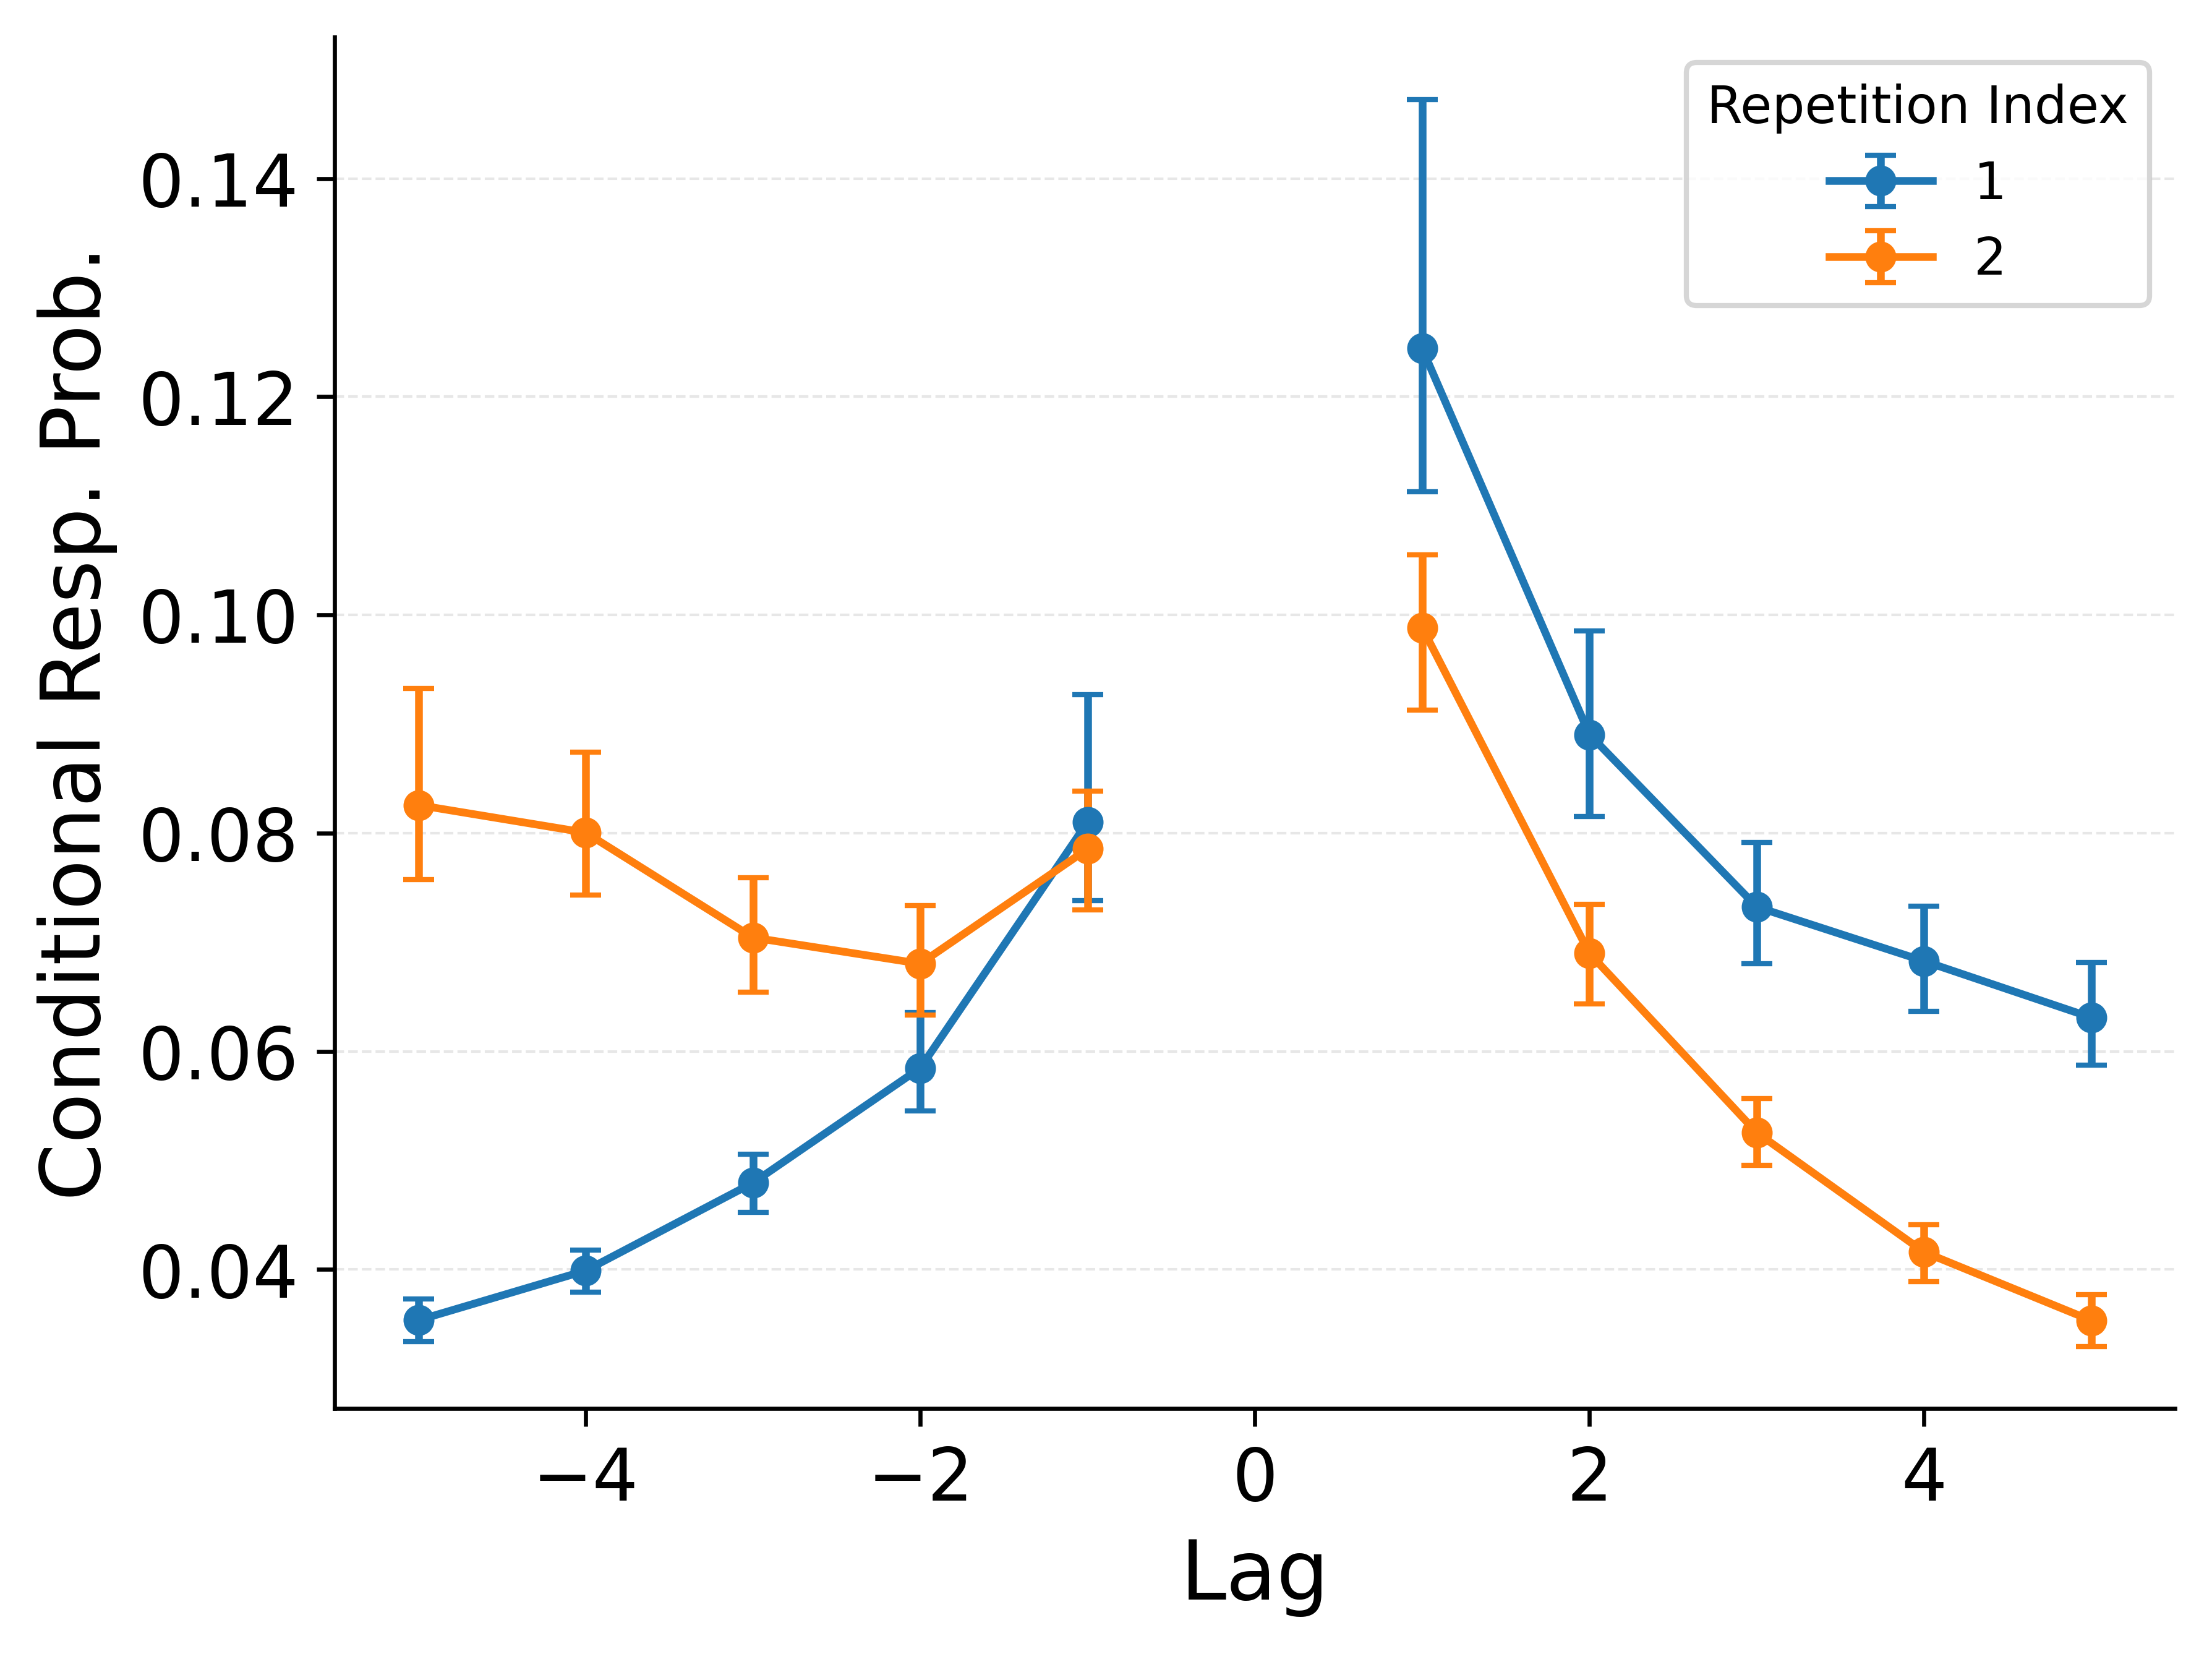
\includegraphics{../../work/thesis/figures/LohnasKahana2014_control_WeirdPositionalCMR_full_best_of_3_LT4_rep_crp.png}\end{minipage}%

\end{figure}%

Finally, we consider the the serial recall variant of this analysis to
examine forward chaining in lists with item repetitions. The
occurrence-specific test-phase reinstatement directly targets
cross-occurrence competition in serial report. After correct report
through the first occurrence at \(i\), Instance-CMR maintains strong
continuations to \(i{+}1\) and does not elevate erroneous continuations
to the competitor \(j{+}1\) relative to baseline
(Figure~Figure~\ref{fig-os_serial_rep_crp}, bottom row)---matching the
non-interference seen in both serial datasets (cf.~top row of
Figure~\ref{fig-serial_rep_crp}). In other words, when the task demands
a specific next item, routing through a single occurrence avoids the
cross-occurrence forward error predicted by blended reinstatement.

\begin{figure}

\caption{\label{fig-os_serial_rep_crp}\textbf{Cross-occurrence forward
errors in serial recall (data vs Instance-CMR).} Left: Logan
(\citeproc{ref-logan2021serial}{2021}). Right: Kahana and Jacobs
(\citeproc{ref-kahana2000interresponse}{2000}). \textbf{Top row (data):}
For items studied at positions \(i\) and \(j\), each panel plots the
conditional probability--- after correct report through the first
occurrence at position \(i\) -- of an erroneous transition to the
\emph{second} occurrence's forward neighbors (\(i\!\rightarrow\!j{+}1\)
and \(i\!\rightarrow\!j{+}2\)), contrasting mixed lists with their
position-matched, symmetric baseline. \textbf{Bottom row (CMR-OS):}
Occurrence-Specific CMR simulations fitted separately to each dataset
and scored with the identical baseline procedure.}

\begin{minipage}{0.50\linewidth}
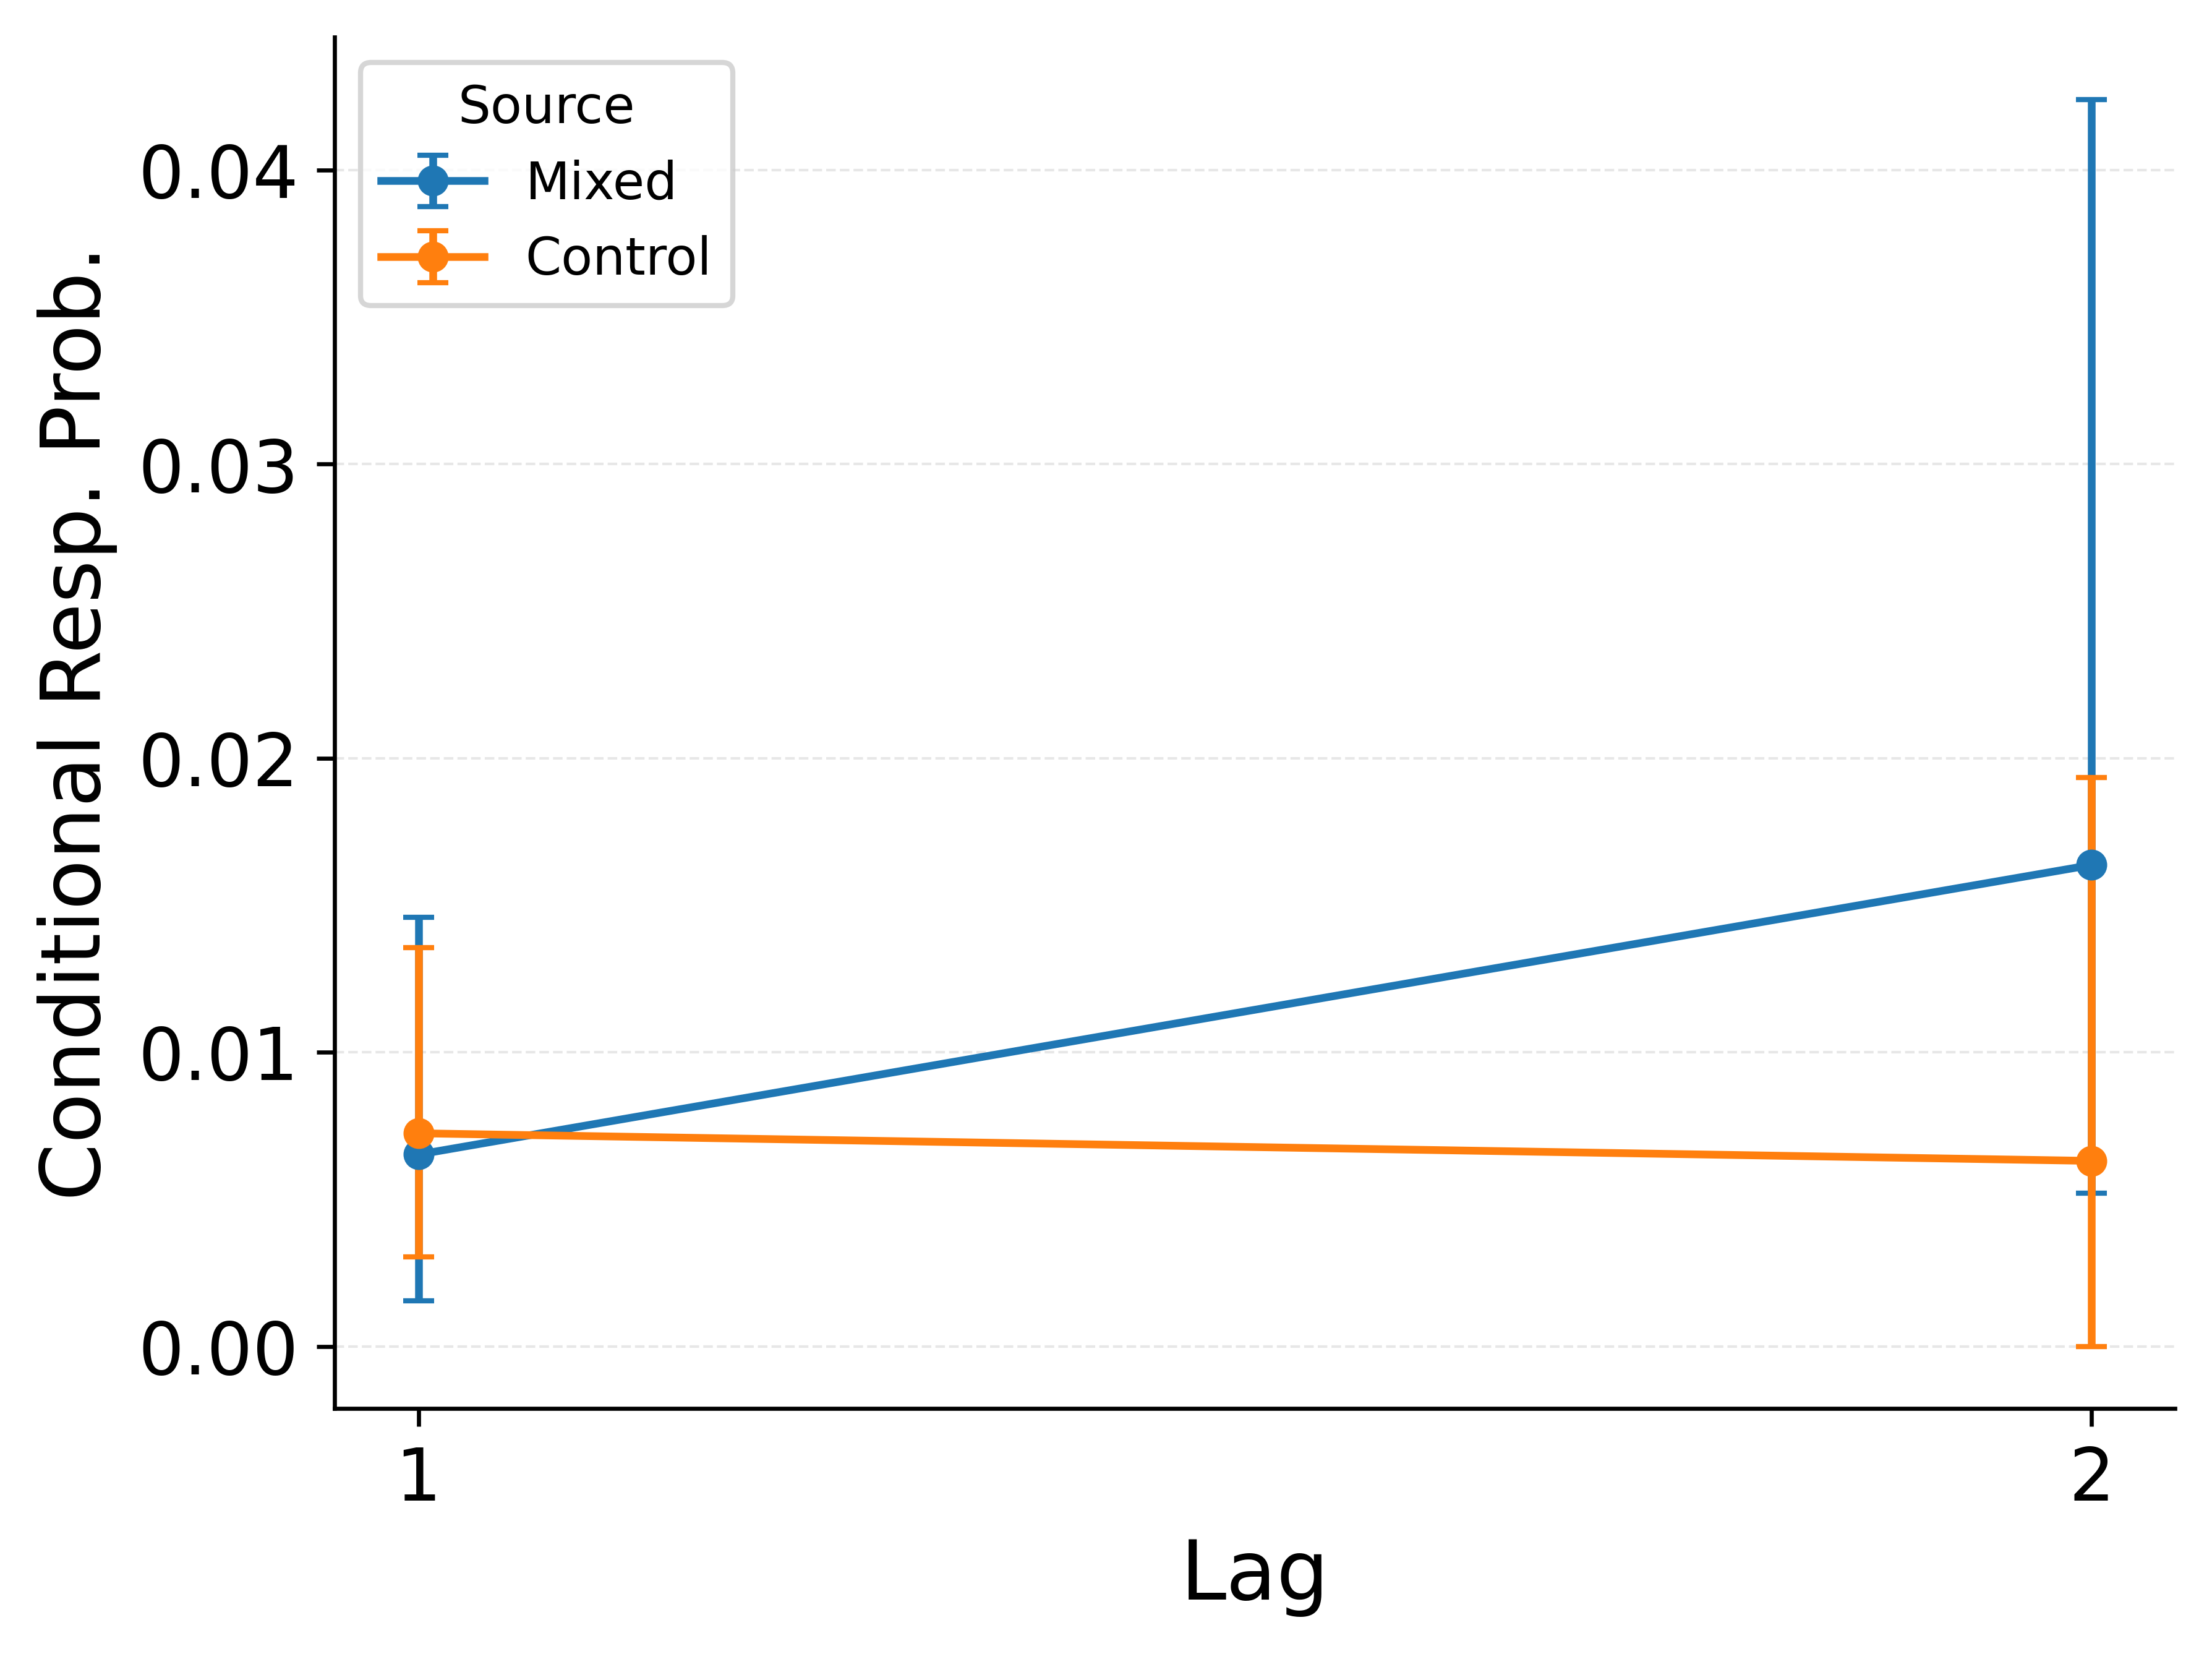
\includegraphics{../../work/thesis/figures/RepeatedRecallsGordonRanschburg2021_mixedvscontrolA_data_full_best_of_3_second_rep_crp.png}\end{minipage}%
%
\begin{minipage}{0.50\linewidth}
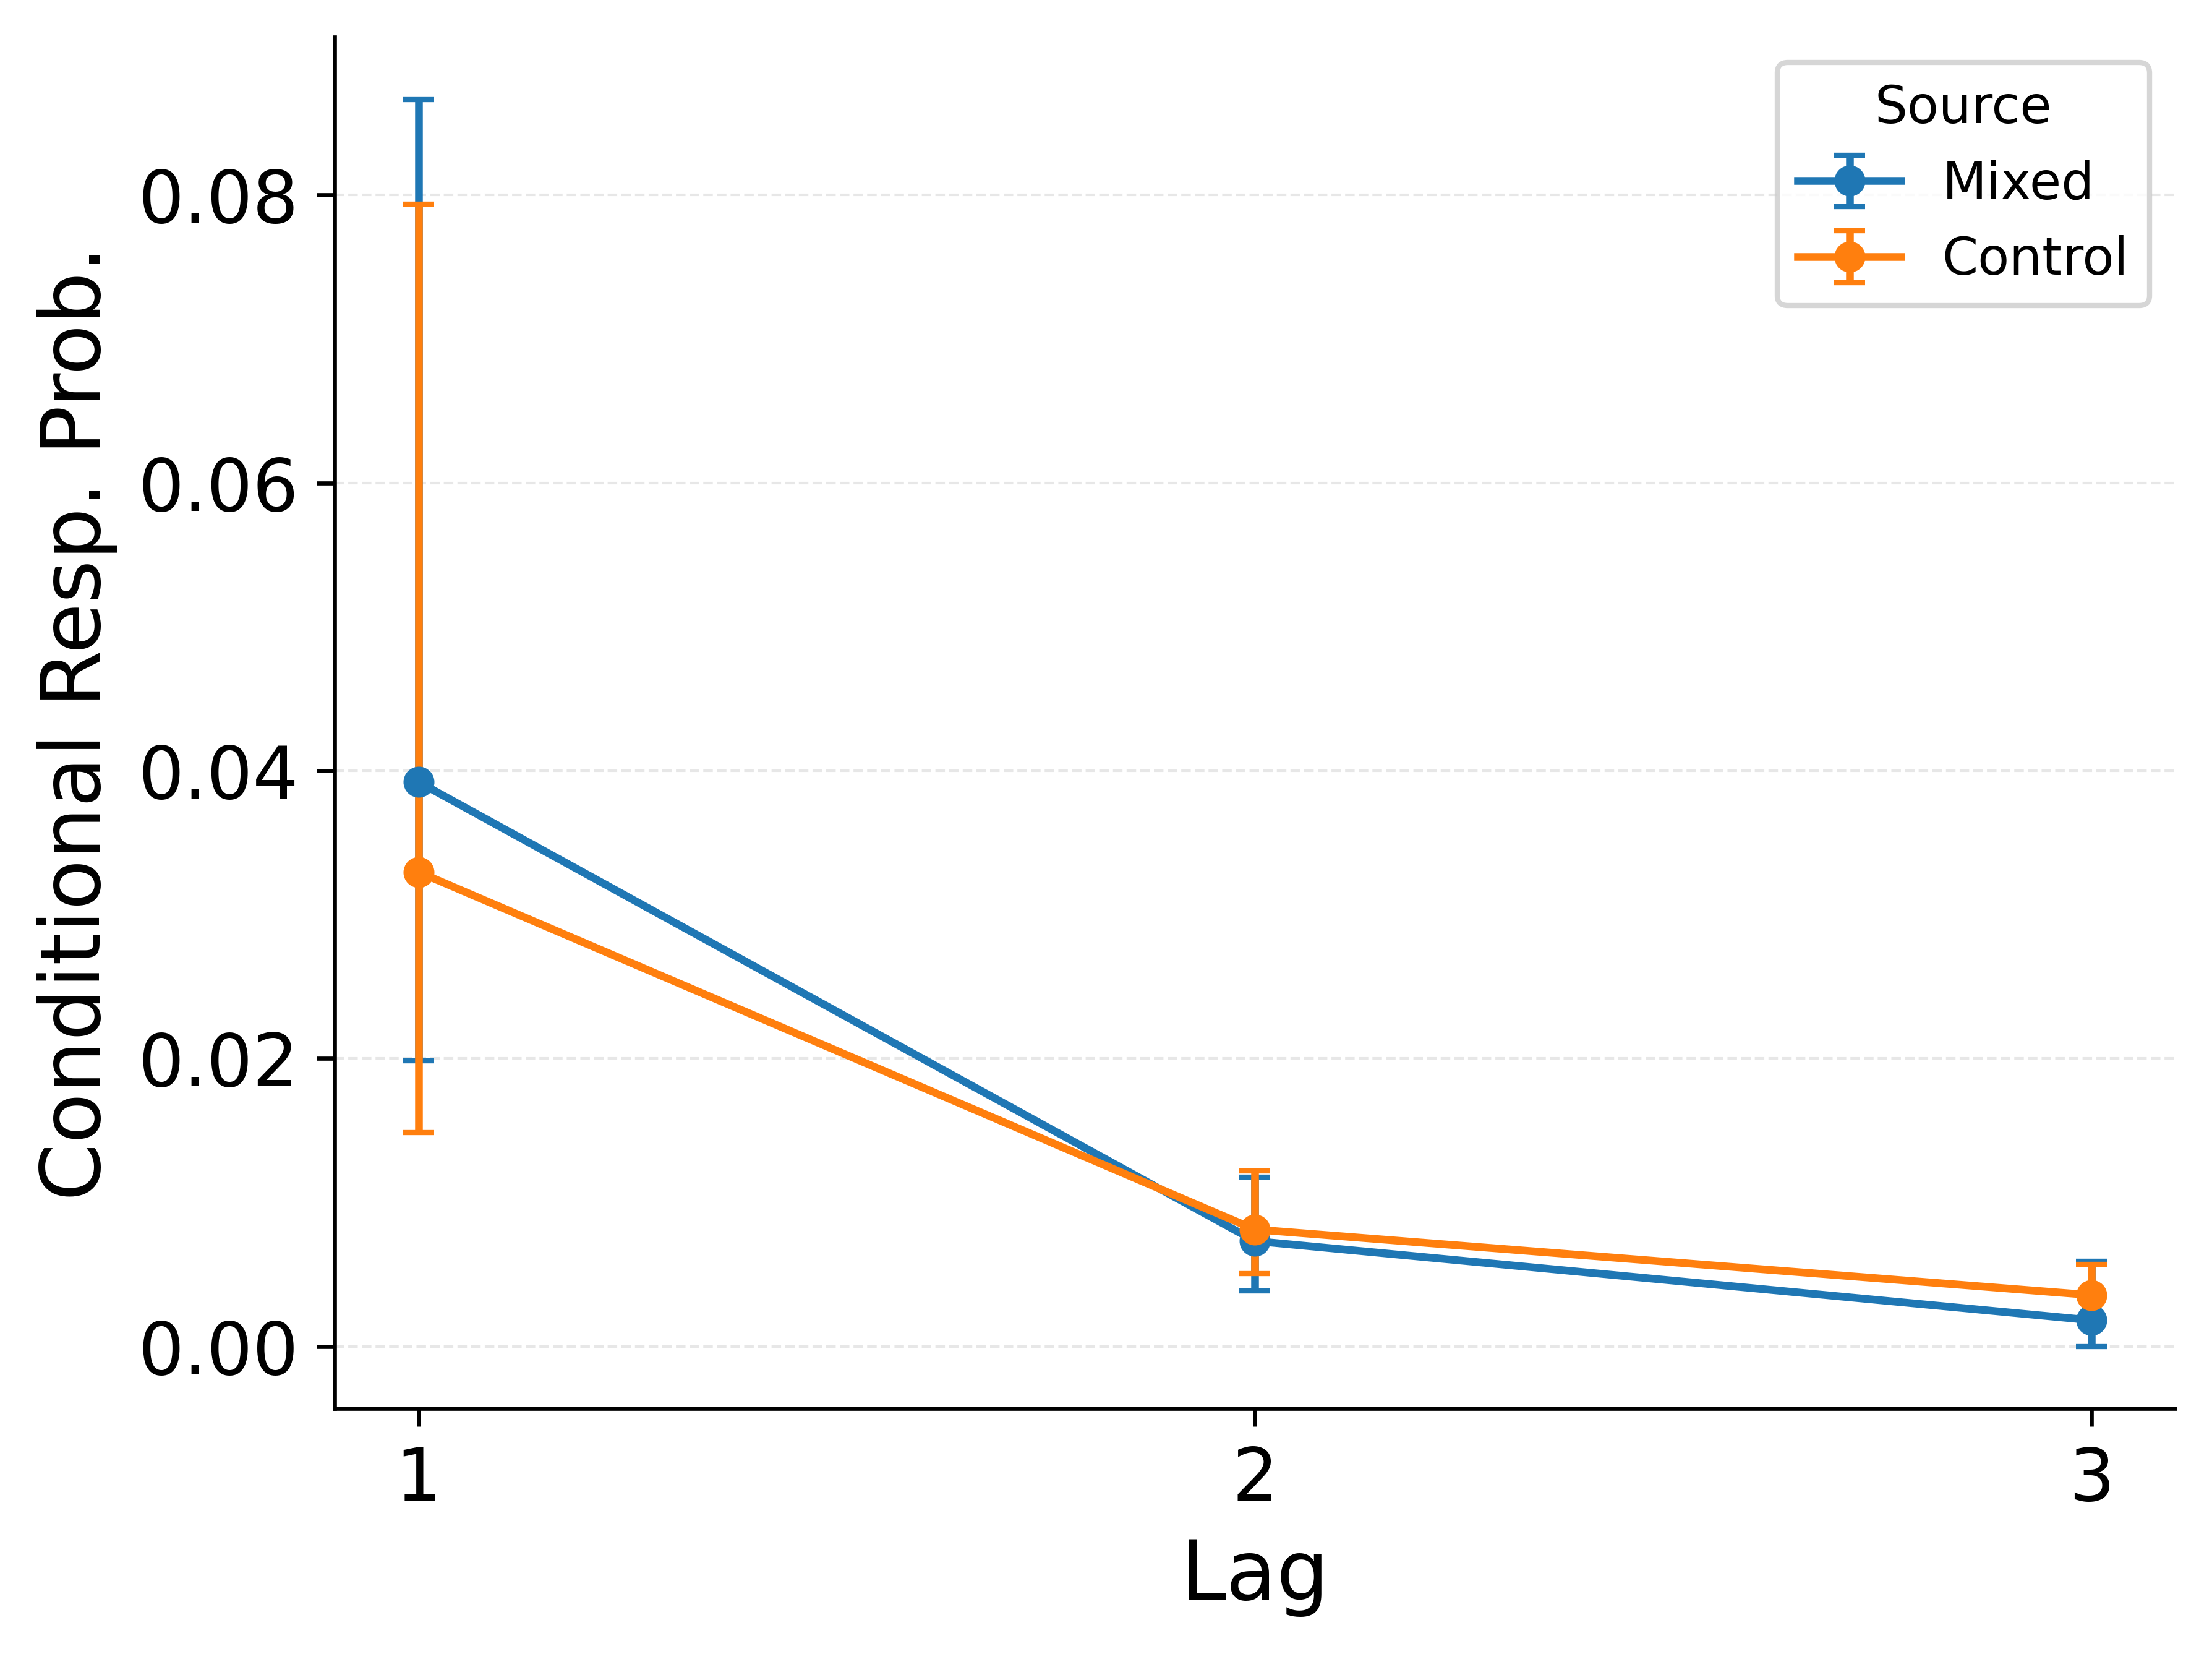
\includegraphics{../../work/thesis/figures/RepeatedRecallsKahanaJacobs2000_mixedvscontrolA_data_full_best_of_3_second_rep_crp.png}\end{minipage}%
\newline
\begin{minipage}{0.50\linewidth}
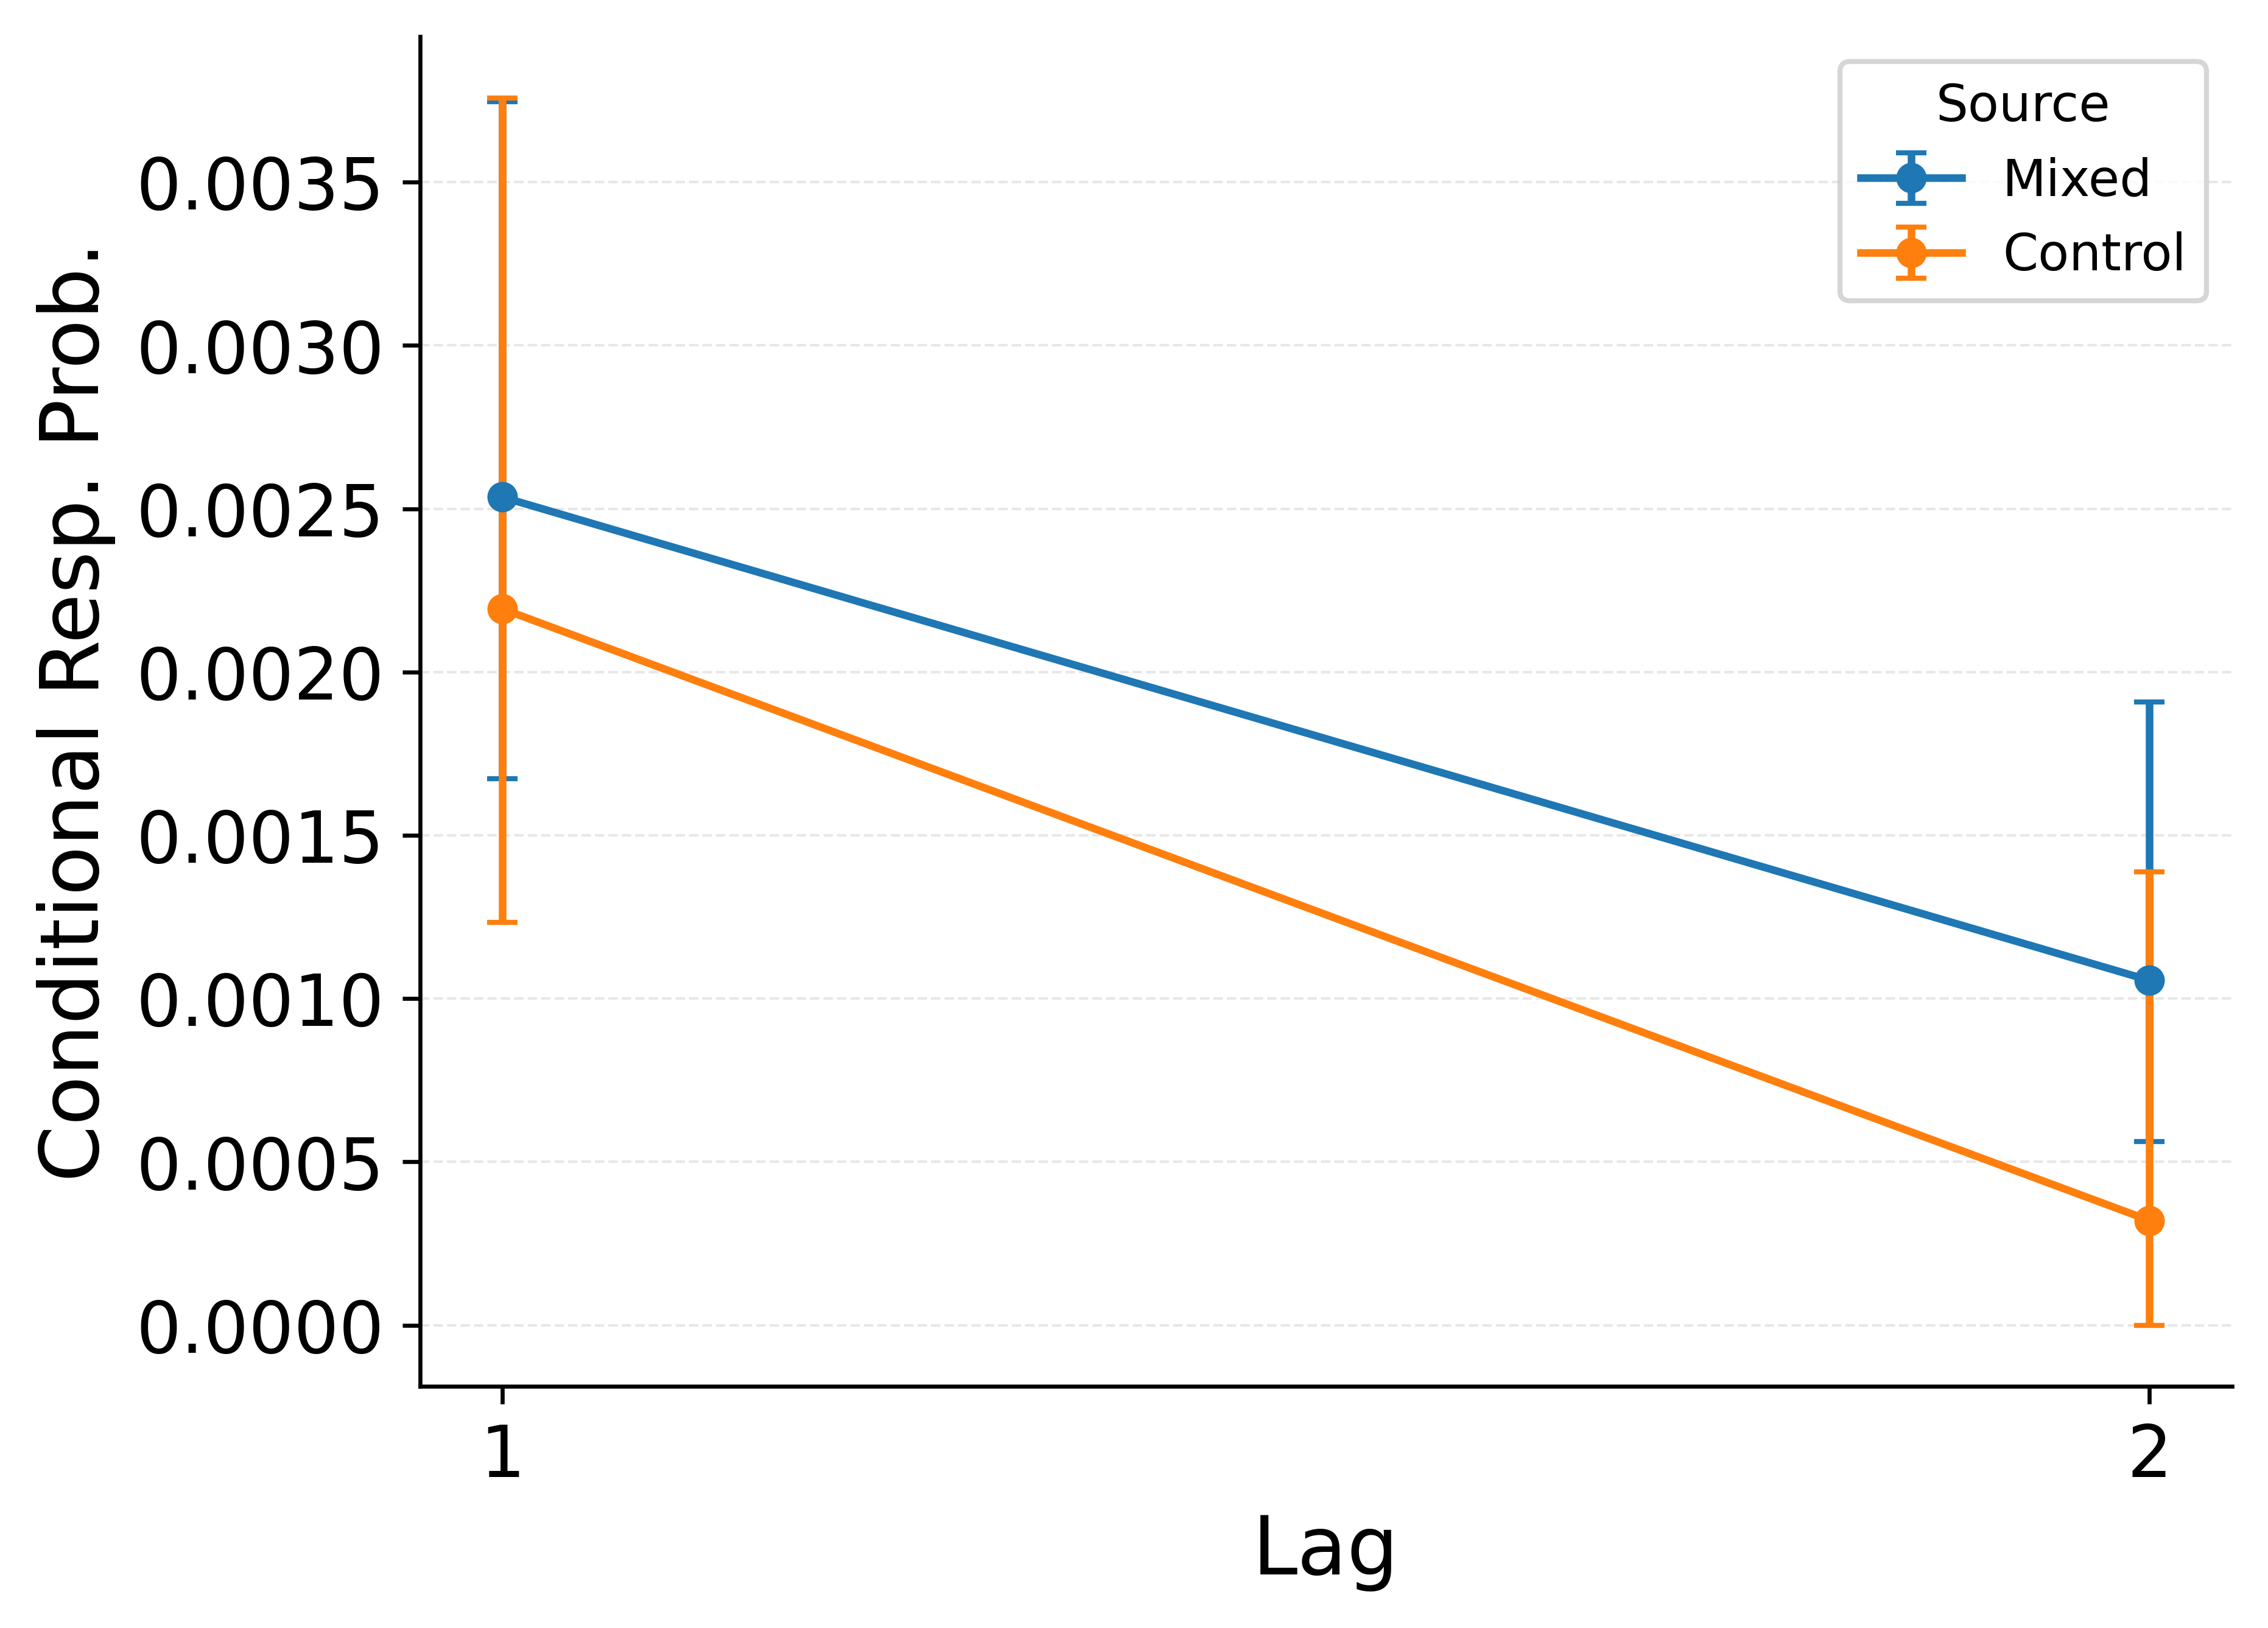
\includegraphics{../../work/thesis/figures/RepeatedRecallsGordonRanschburg2021_mixedvscontrolA_WeirdPositionalCMR_full_best_of_3_second_rep_crp.png}\end{minipage}%
%
\begin{minipage}{0.50\linewidth}
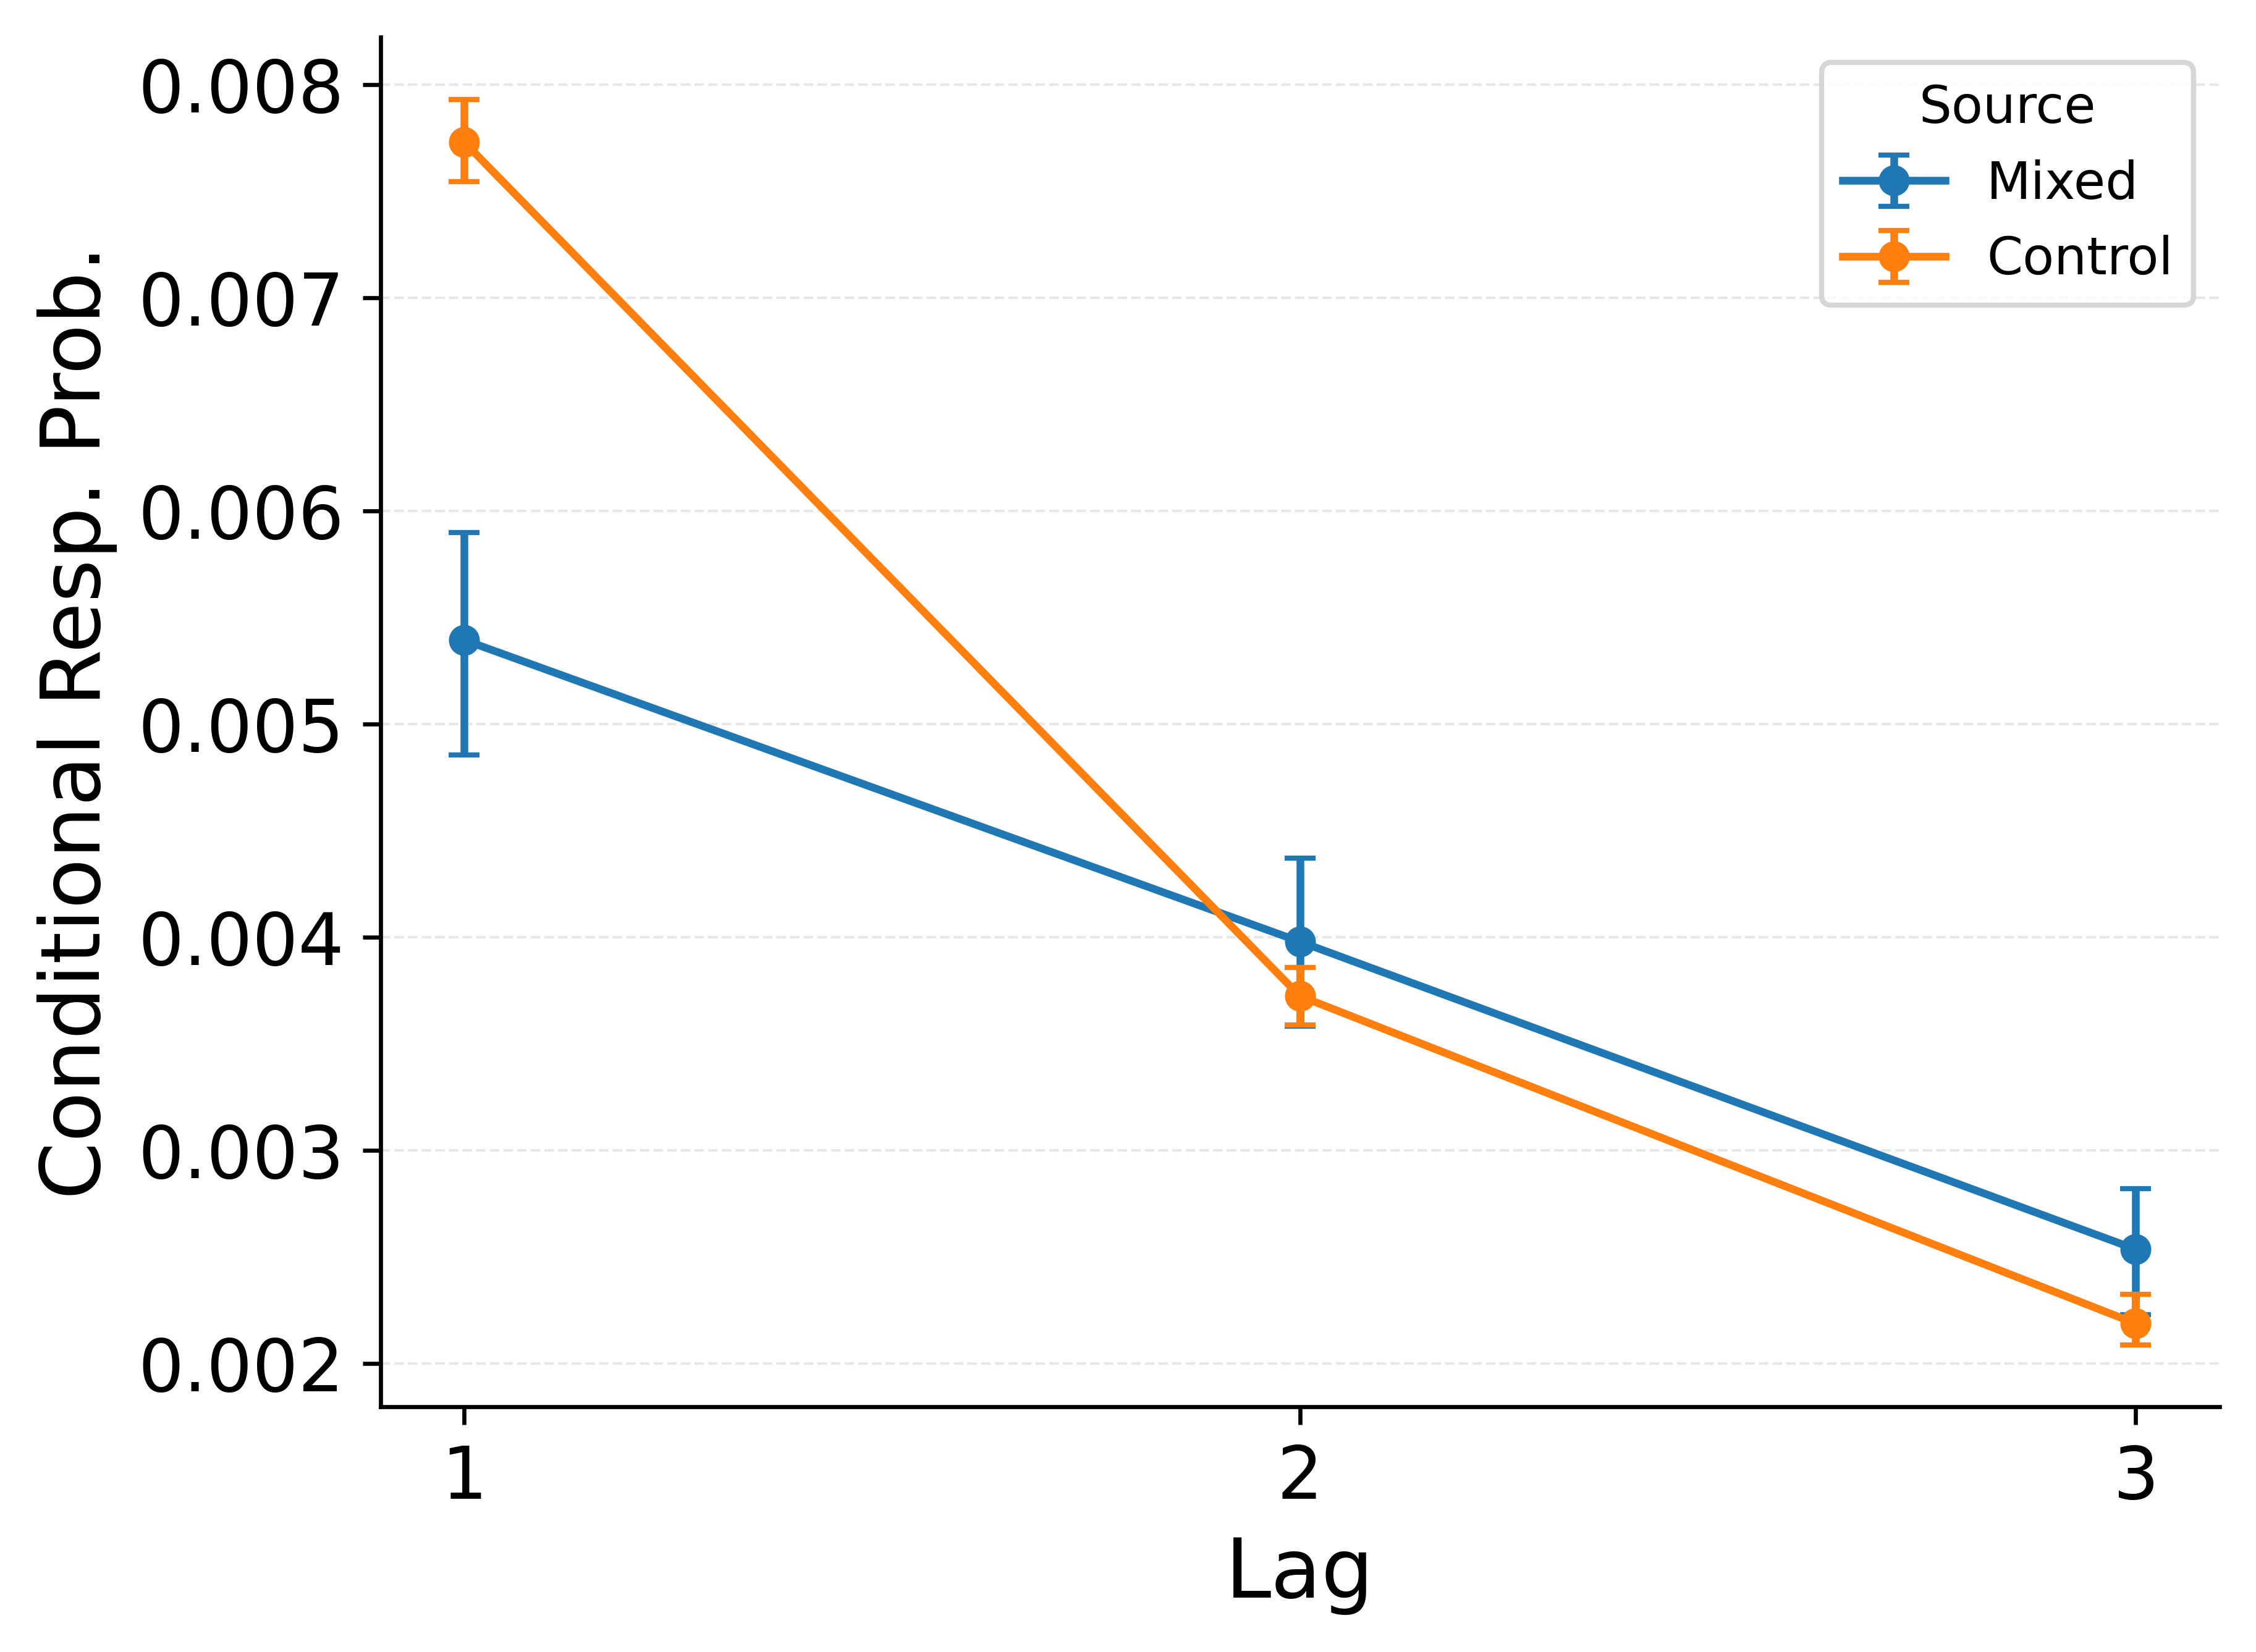
\includegraphics{../../work/thesis/figures/RepeatedRecallsKahanaJacobs2000_mixedvscontrolA_WeirdPositionalCMR_full_best_of_3_second_rep_crp.png}\end{minipage}%

\end{figure}%

Instance-CMR reconciles retrieved-context theory with the absence of
associative interference: it keeps occurrences separate at study and
allows retrieval to select a single occurrence's context at test. It
preserves benchmark fits, removes cross-neighbor linkage, restores
first-over-second separation in the outgoing repetition lag-CRP, and
eliminates cross-occurrence forward errors in serial recall. What it
does not capture are the systematic boosts for the first occurrence
evident in (i) the selective lag-0 elevation in the neighbor-contiguity
test (first-neighborhood triggers), (ii) the larger first-over-second
asymmetry on the incoming repetition lag-CRP, and (iii) the boosted
separation on the outgoing repetition lag-CRP beyond baseline (cf.
Figure~\ref{fig-neighbor_contiguity},
Figure~\ref{fig-backward_rep_lag_crp},
Figure~\ref{fig-repetition_lag_crp}). These residual asymmetries
motivate an additional mechanism that preferentially strengthens the
first-occurrence trace \emph{without} knitting contexts
together---developed next in the ICMR-Reinf variant.

\section{Exploring Reinforcement without Associative Blending at
Study}\label{exploring-reinforcement-without-associative-blending-at-study}

ICMR-Reinf addresses the residual asymmetries by reconceptualizing
study-phase retrieval as reinforcement rather than reinstatement. At the
second presentation, the model strengthens the first-occurrence trace
but does not reinstate its contextual features; the two occurrences
therefore remain contextually distinct at encoding, exactly as in
CMR-NoSPR and Instance-CMR. At test, ICMR-Reinf retains Instance-CMR's
occurrence-specific reinstatement: when a repeated item is recalled, a
single occurrence's context is selectively reinstated (governed by the
same trace-sensitivity used in the recall competition; no new degrees of
freedom there). The only added degree of freedom in this variant is a
single reinforcement factor bounded between ``no strengthening'' and
``match the original trace's strength.'' The questions are whether
ICMR-Reinf (i) preserves benchmark free-recall behavior and the spacing
function, (ii) maintains the elimination of cross-occurrence neighbor
knitting, (iii) not only removes balanced access in the outgoing
repetition lag-CRP but boosts the first-over-second separation in mixed
lists beyond baseline (as in the data), and (iv) preserves the
non-interference pattern in serial recall.

ICMR-Reinf maintains good agreement with serial-position, lag-CRP, and
first-recall profiles under the same matched, symmetric scoring used
throughout. As with prior variants, mixed--control differences are
minimal once the baseline is applied
(Figure~\ref{fig-icmr_reinf_benchmarks}). Thus, adding reinforcement at
study does not degrade core free-recall benchmarks.

\begin{figure}

\caption{\label{fig-icmr_reinf_benchmarks}ICMR-Reinf benchmarks (free
recall). Simulated serial-position curves (SPC; top left), lag-CRP (top
right), and probability of first/next recall (bottom) for mixed vs
matched-control lists from Lohnas and Kahana
(\citeproc{ref-lohnas2014retrieved}{2014}) under symmetric scoring.
Reinforcement at study preserves benchmark fits.}

\begin{minipage}{0.50\linewidth}
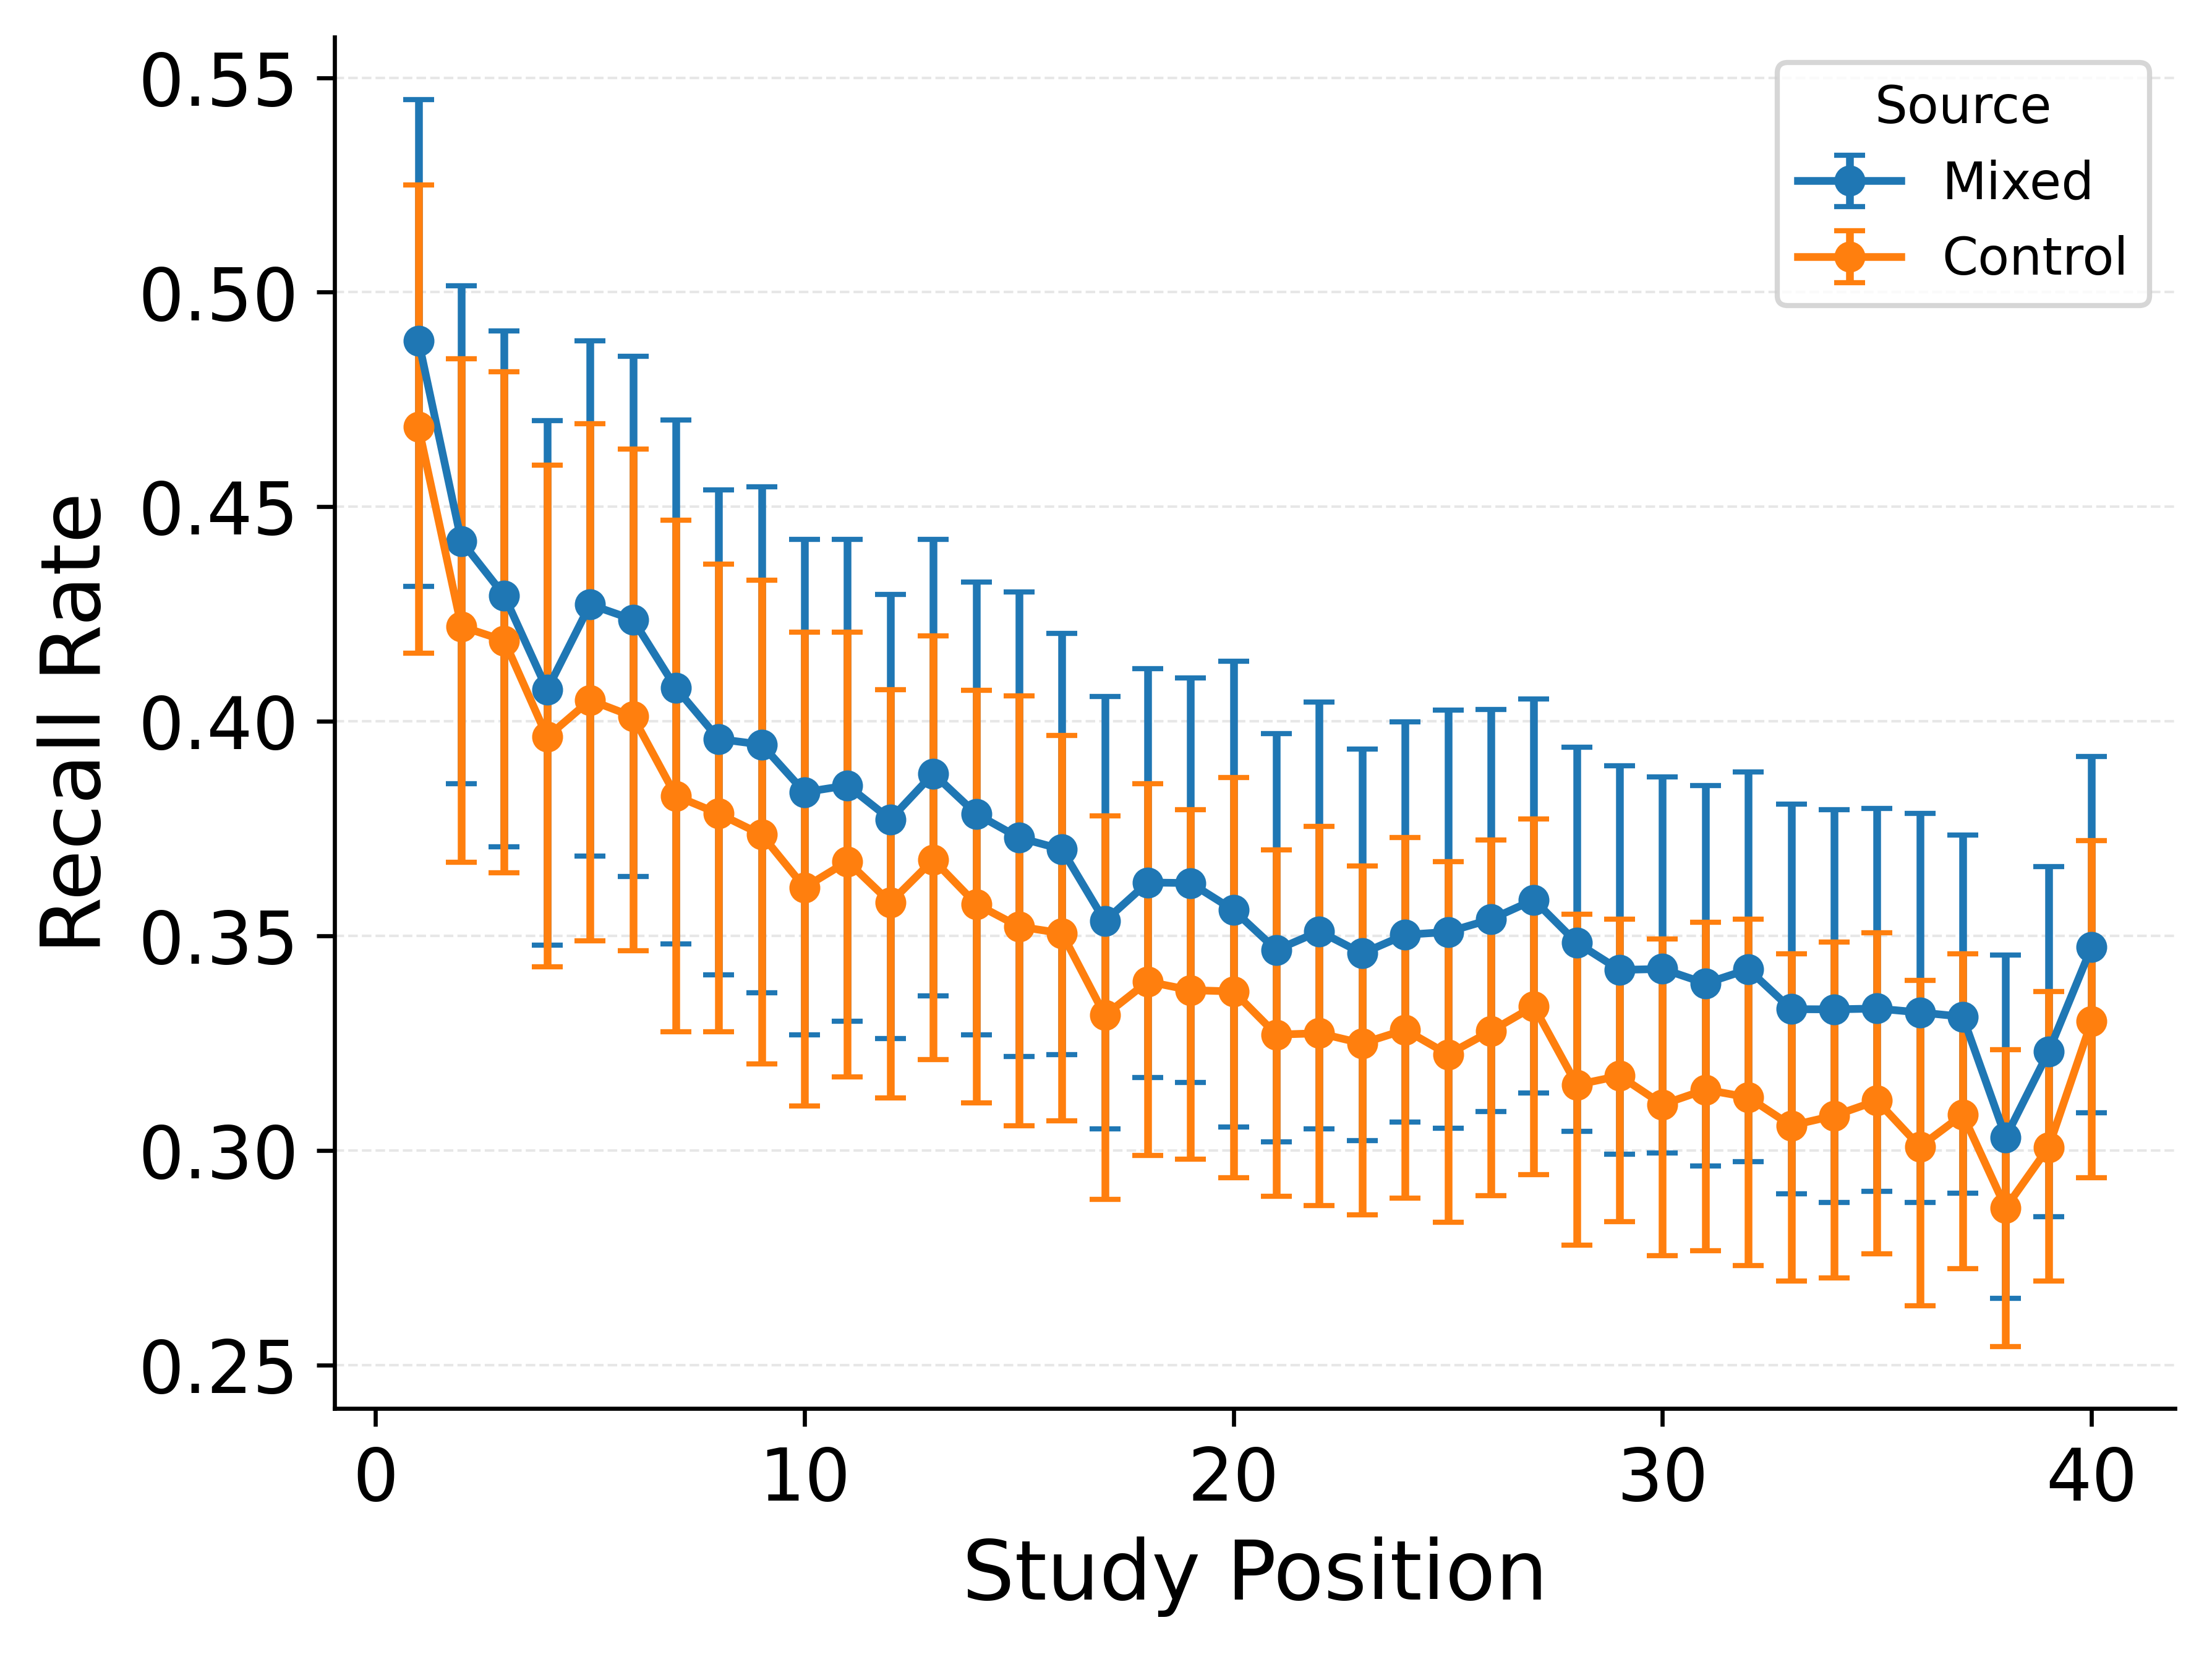
\includegraphics{../../work/thesis/figures/LohnasKahana2014_mixedvscontrolA_WeirdReinfPositionalCMR_full_best_of_3_LT4_spc.png}\end{minipage}%
%
\begin{minipage}{0.50\linewidth}
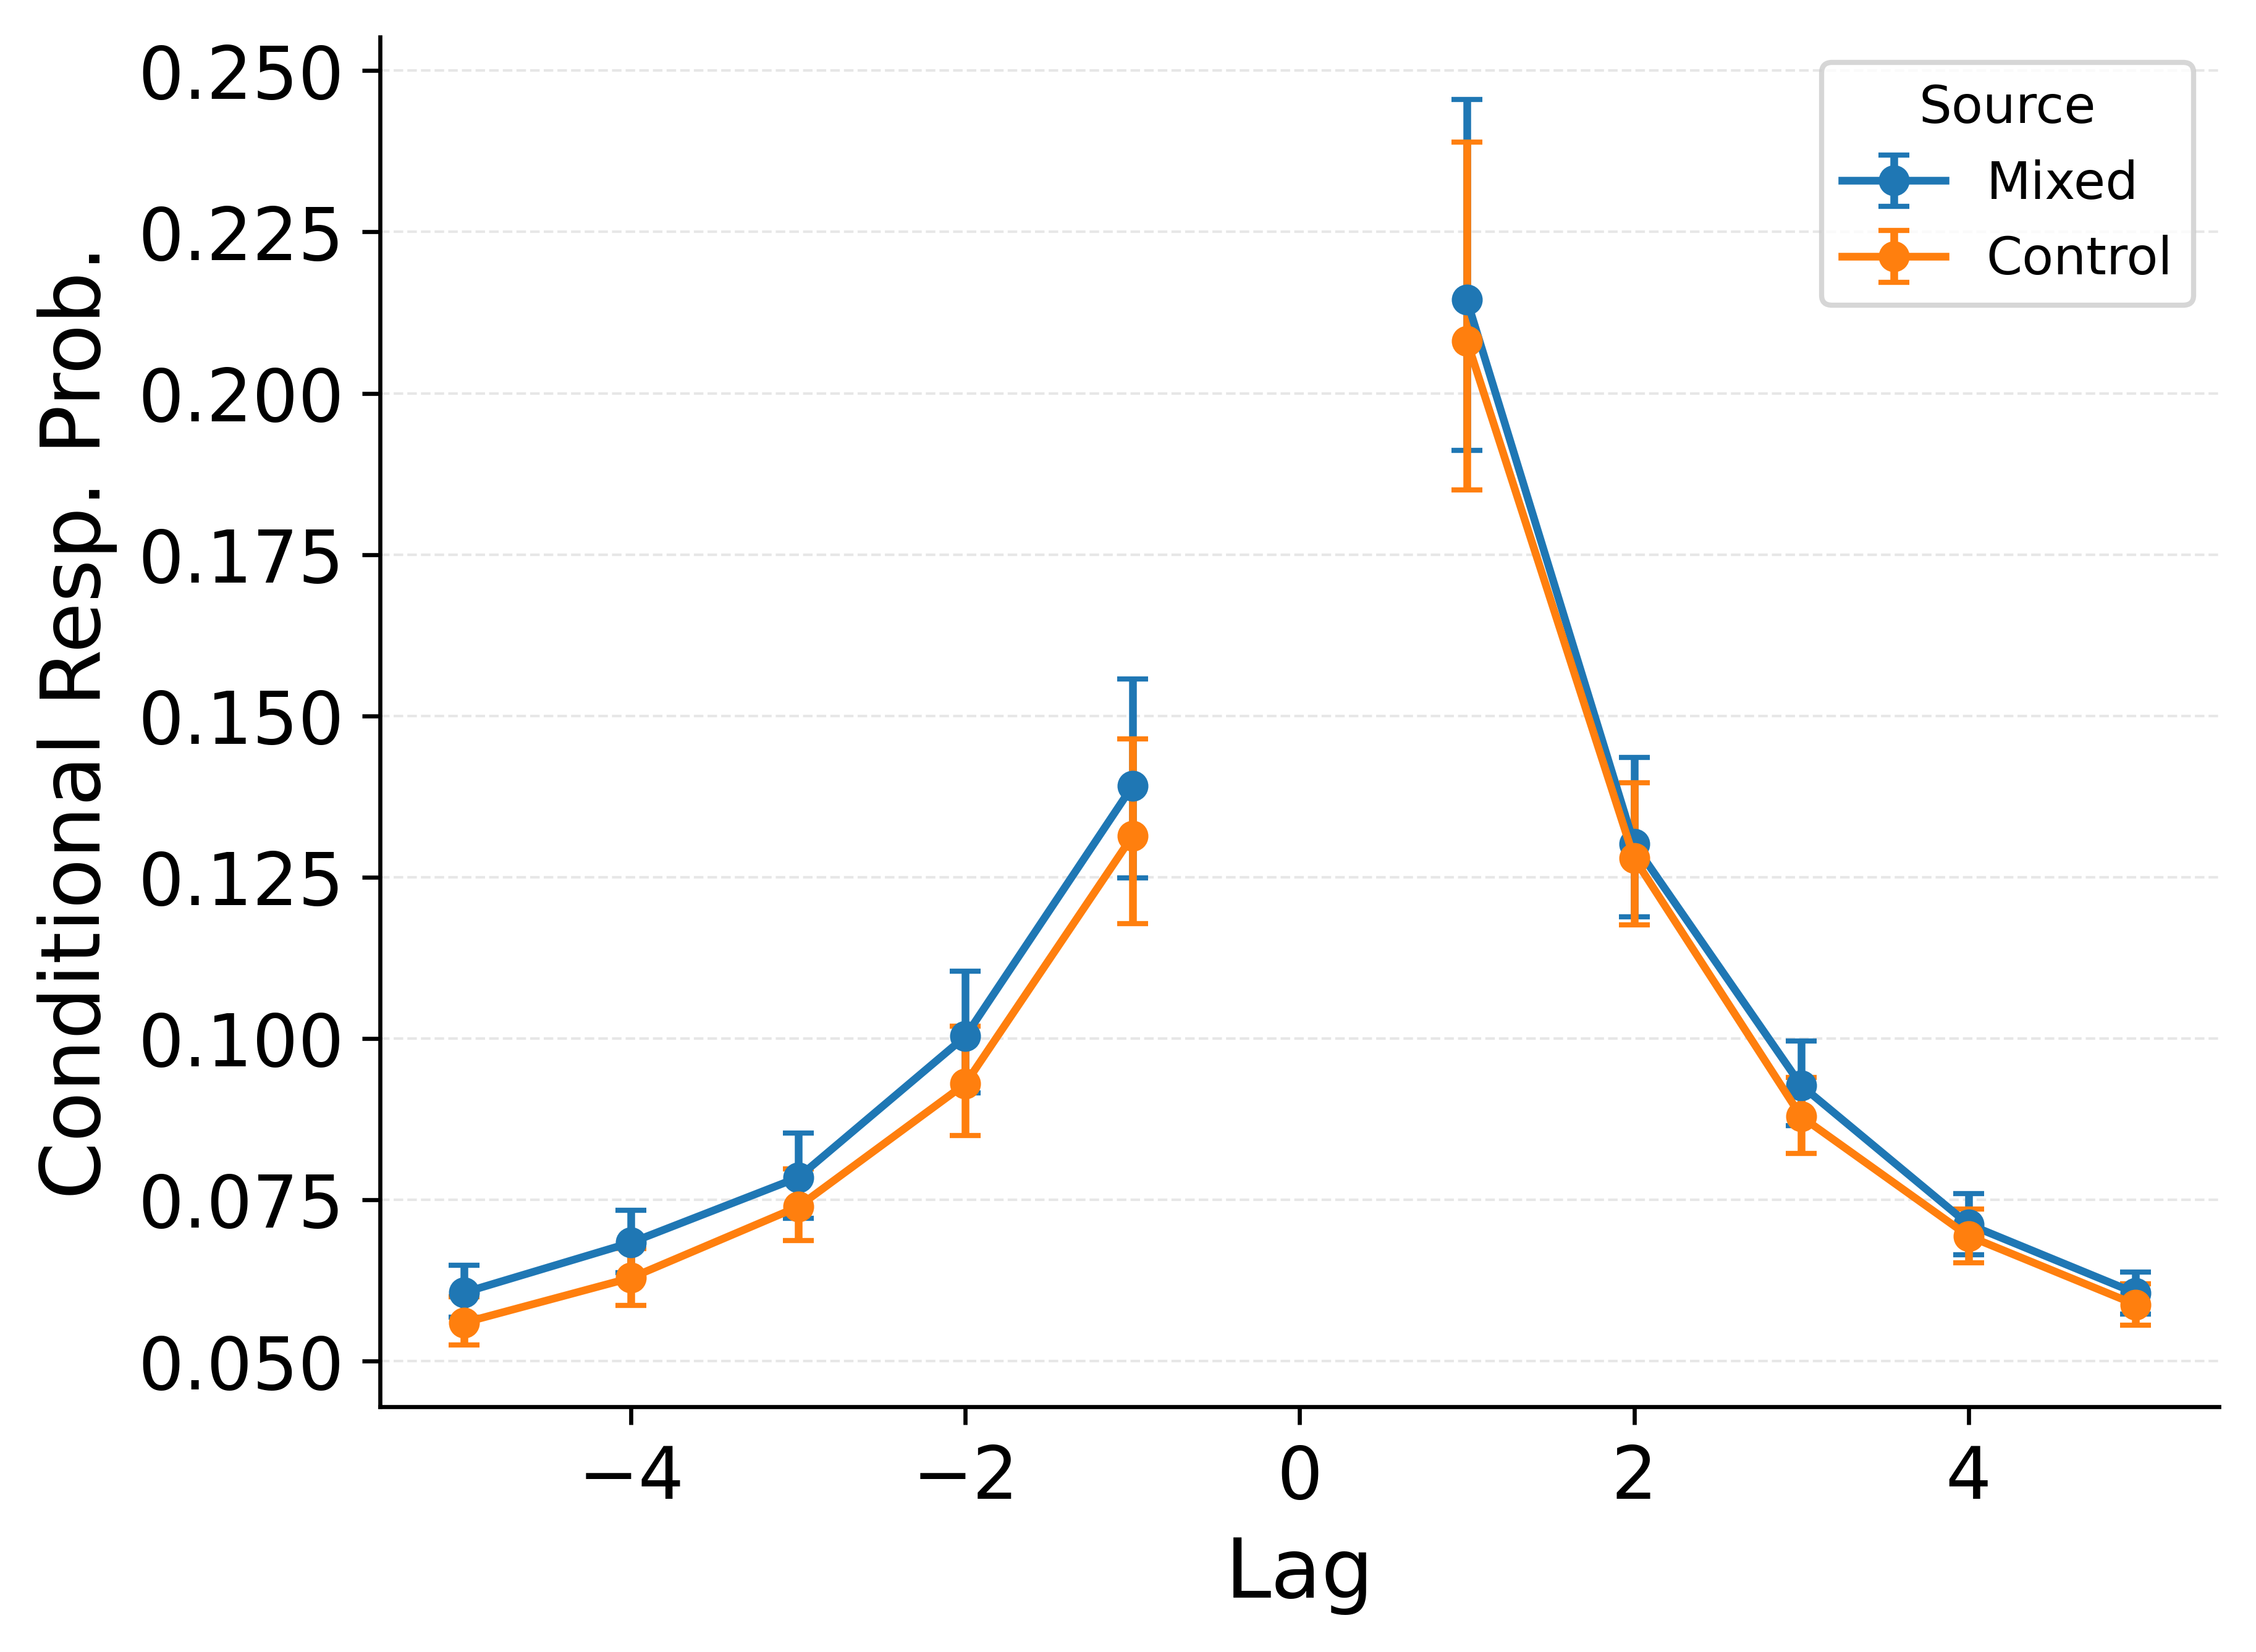
\includegraphics{../../work/thesis/figures/LohnasKahana2014_mixedvscontrolA_WeirdReinfPositionalCMR_full_best_of_3_LT4_crp.png}\end{minipage}%
\newline
\begin{minipage}{\linewidth}
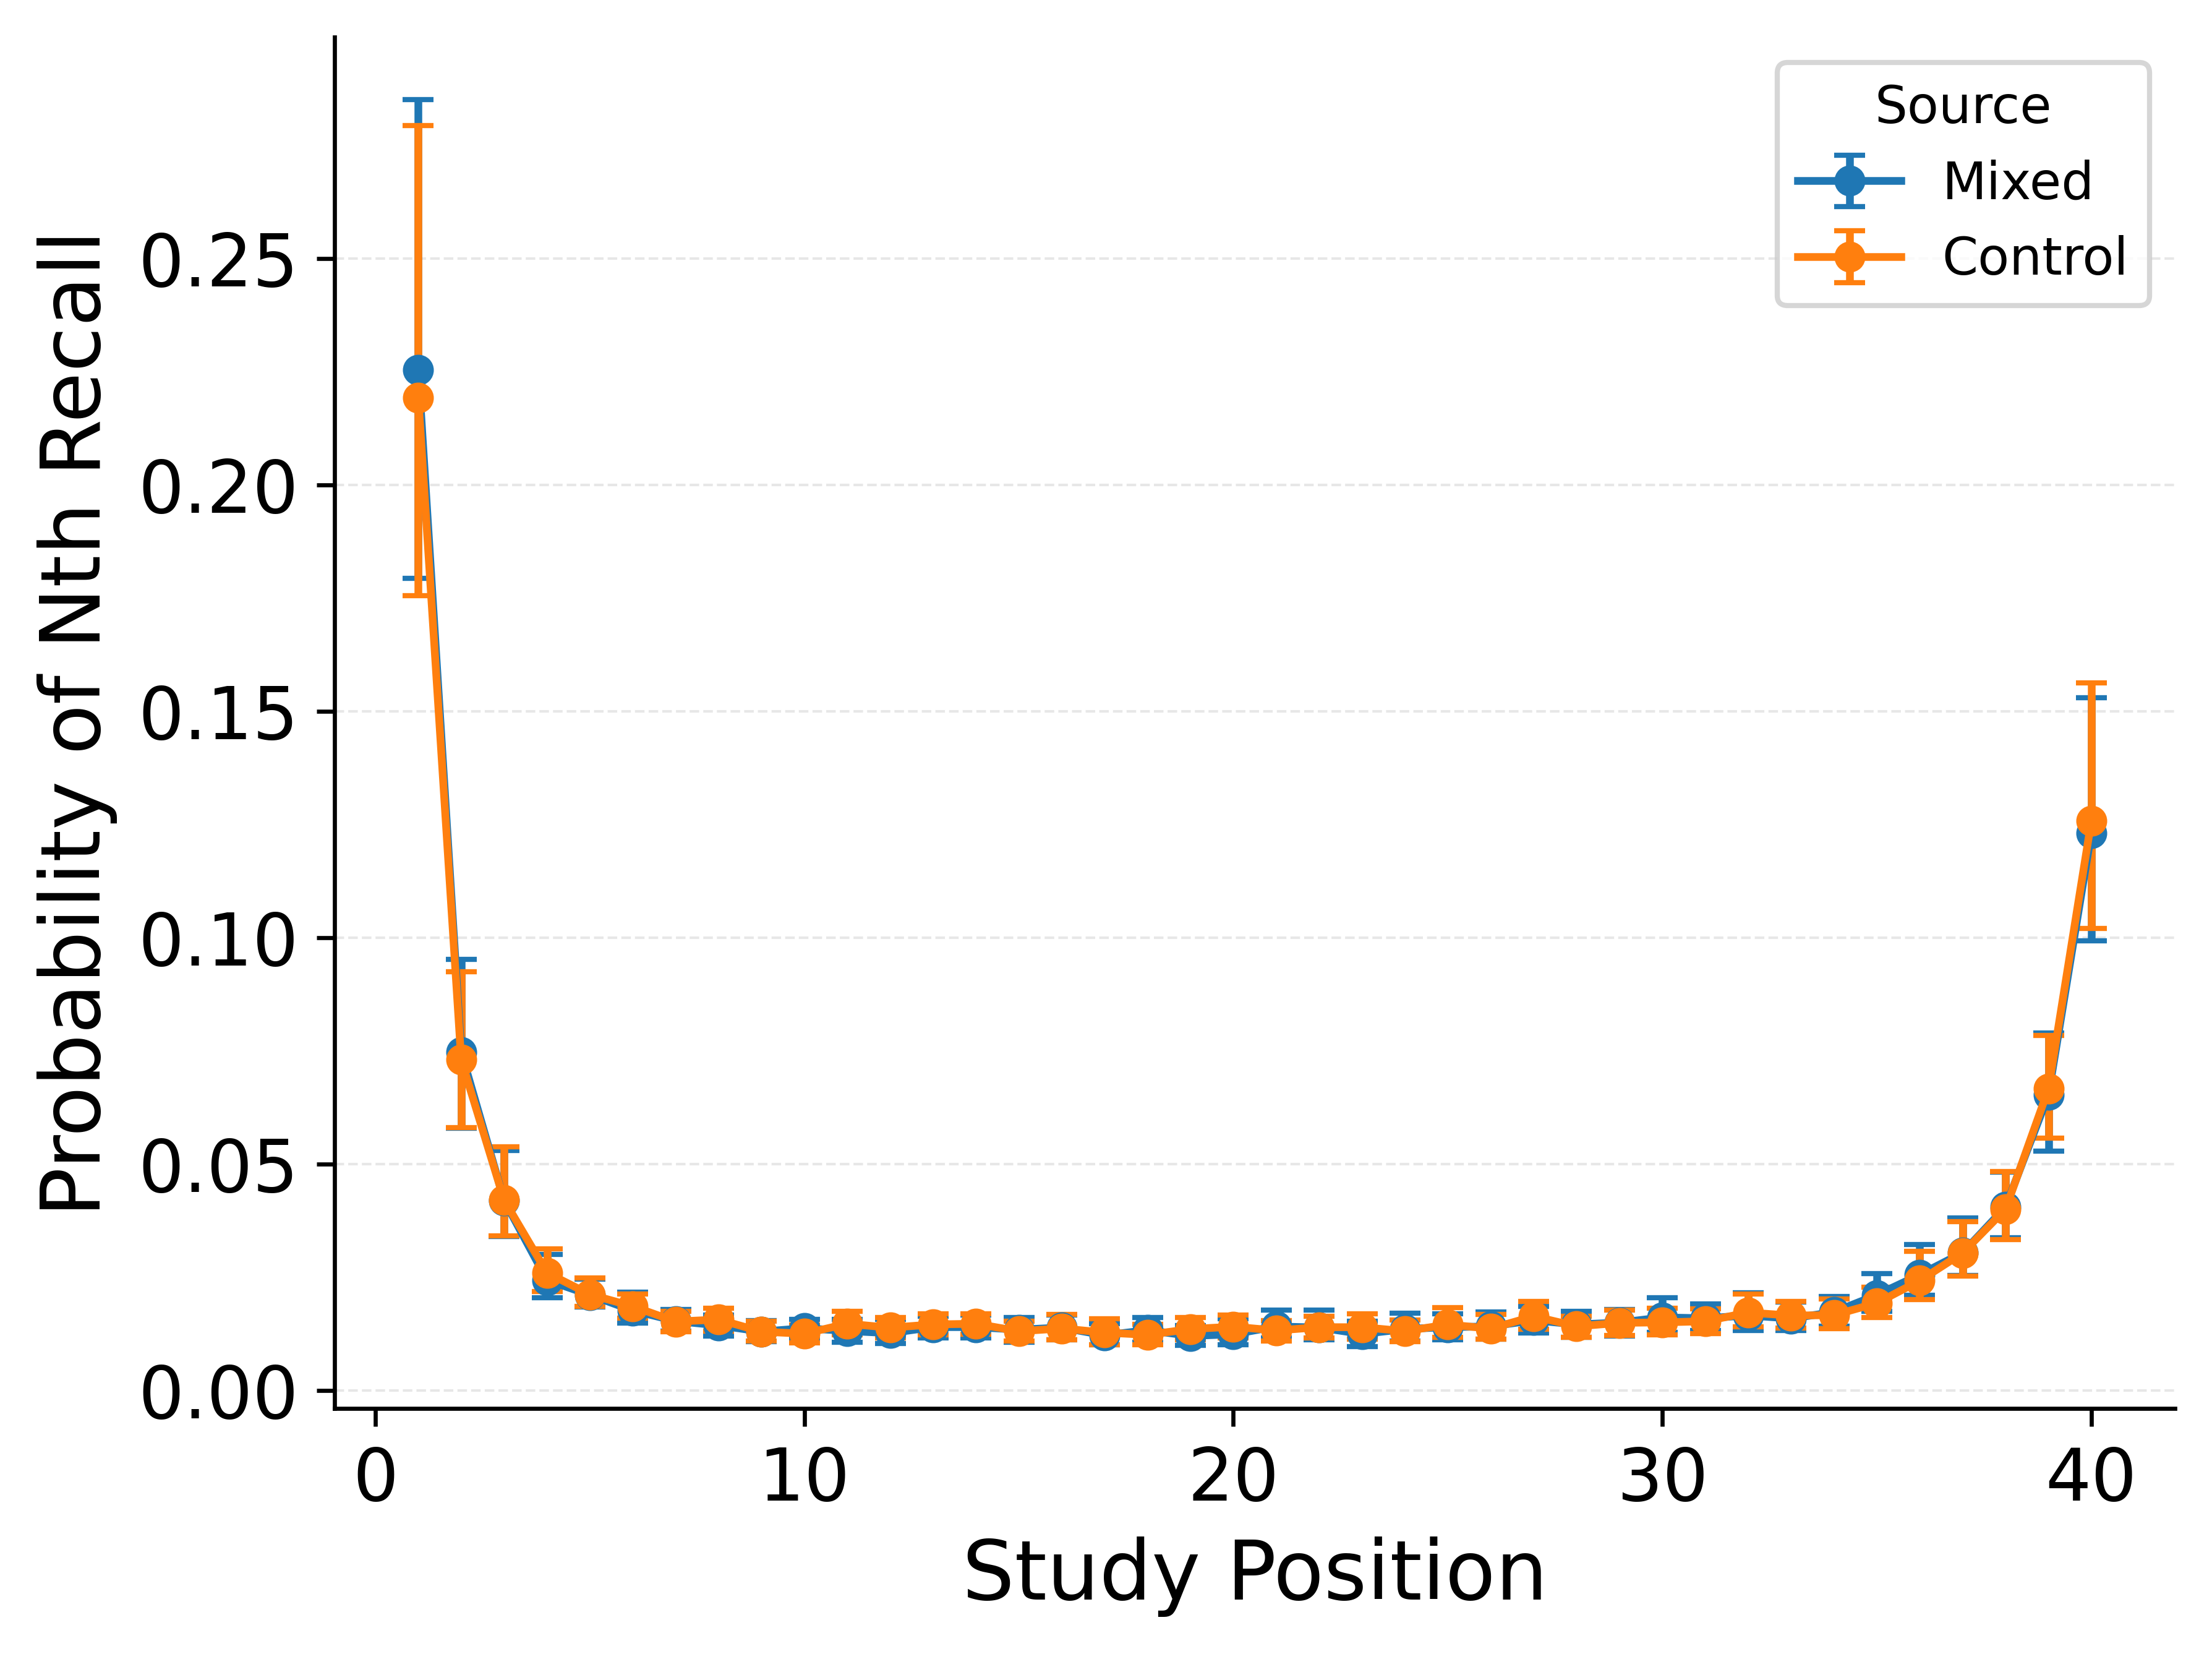
\includegraphics{../../work/thesis/figures/LohnasKahana2014_mixedvscontrolA_WeirdReinfPositionalCMR_full_best_of_3_LT4_pnr.png}\end{minipage}%

\end{figure}%

Like the other variants, ICMR-Reinf reproduces a robust, monotonic
spacing advantage (Figure~\ref{fig-icmr_reinf_spacing}). Reinforcement
does not blunt spacing; the basic lag-dependent memorability gain
remains intact. (As with Instance-CMR, the model does not by itself
reproduce the steeper mixed-list slope observed in the data; cf.
Figure~\ref{fig-spacing}.)

\begin{figure}

\caption{\label{fig-icmr_reinf_spacing}ICMR-Reinf spacing function.
Simulated spacing curves for mixed vs matched-control lists from Lohnas
and Kahana (\citeproc{ref-lohnas2014retrieved}{2014}). The spacing
advantage is preserved; the model does not, by itself, produce the
additional steepening seen in mixed lists (cf.
Figure~\ref{fig-spacing}).}

\begin{minipage}{\linewidth}

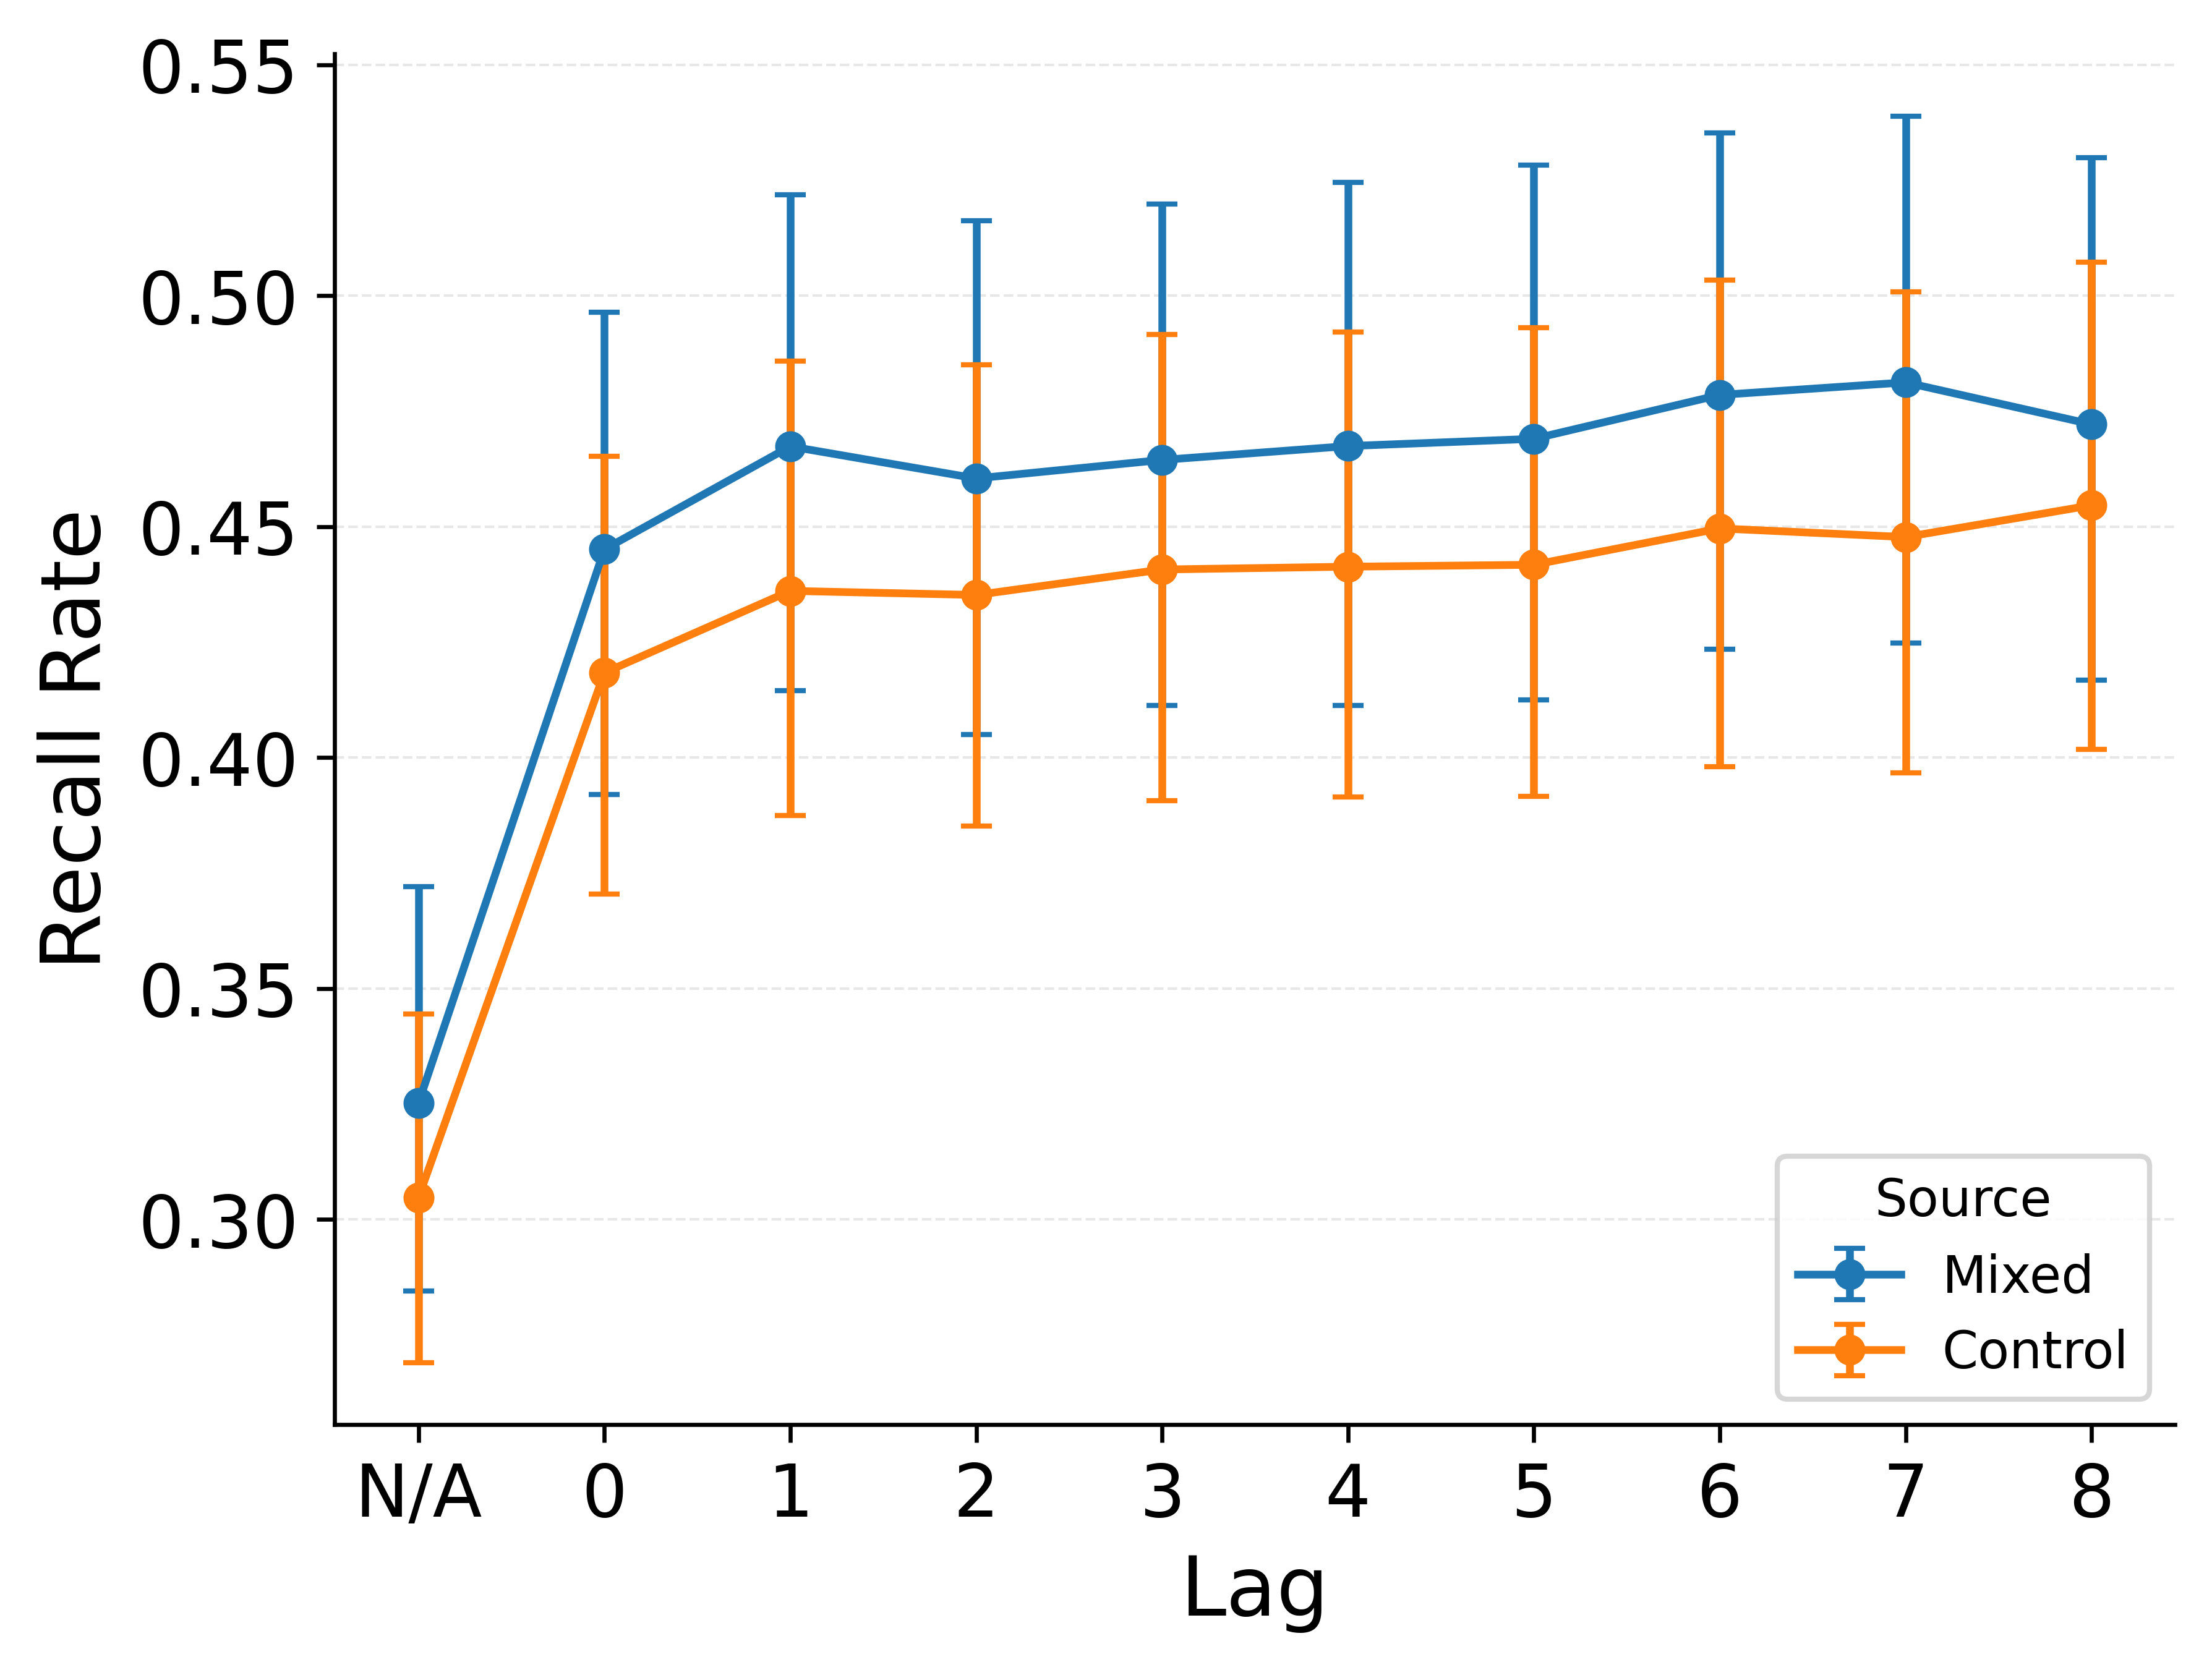
\includegraphics{../../work/thesis/figures/LohnasKahana2014_mixedvscontrolA_WeirdReinfPositionalCMR_full_best_of_3_LT4_full_rpl.png}

\end{minipage}%

\end{figure}%

However, ICMR-Reinf potentially boosts recall rates for items studied at
mid-list positions and for repeated items compared to control list items
in the spacing curve, reflecting the consequences of reinforcement on
the first-occurrence trace. A more refined model could -- instead of
boosting memory for repeated items according to a reinforcement
mechanism -- use a more complex balancing of trace strengths across
occurrences to account for enhanced access to first-occurrence contexts
during retrieval.

Turning to cross-occurrence neighbor contiguity, ICMR-Reinf inherits two
ingredients that prevent knitting across neighborhoods: distinctive
contexts at encoding and occurrence-specific reinstatement at test. As a
result, the centered neighbor-contiguity analyses remain flat at the
other occurrence's neighbors (no above-baseline peaks), matching the
data and improving on standard CMR's incorrect elevations. At the same
time, reinforcement selectively boosts lag\,=\,0 in the first→second
variant (triggering from neighbors of the first presentation),
reflecting easier access to the repeated item itself---an asymmetric
feature visible in the data (cf. Figure~\ref{fig-neighbor_contiguity}).

\begin{figure}

\caption{\label{fig-reinf_neighbor_contiguity}ICMR-Reinf:
cross-occurrence neighbor transitions (centered lag-CRPs). Left:
triggers from forward neighbors of the first presentation
(\(i{+}1,i{+}2\)), lags centered on the second (\(\ell=text{next}-j\)).
Right: symmetric variant (triggers \(j{+}1,j{+}2\); lags centered on
\(i\)). Mixed--minus--baseline curves remain flat at the other
occurrence's neighbors (no knitting). A selective lag\,=\,0 elevation
emerges in the first→second variant, consistent with boosted access to
the repeated item itself.}

\begin{minipage}{0.50\linewidth}
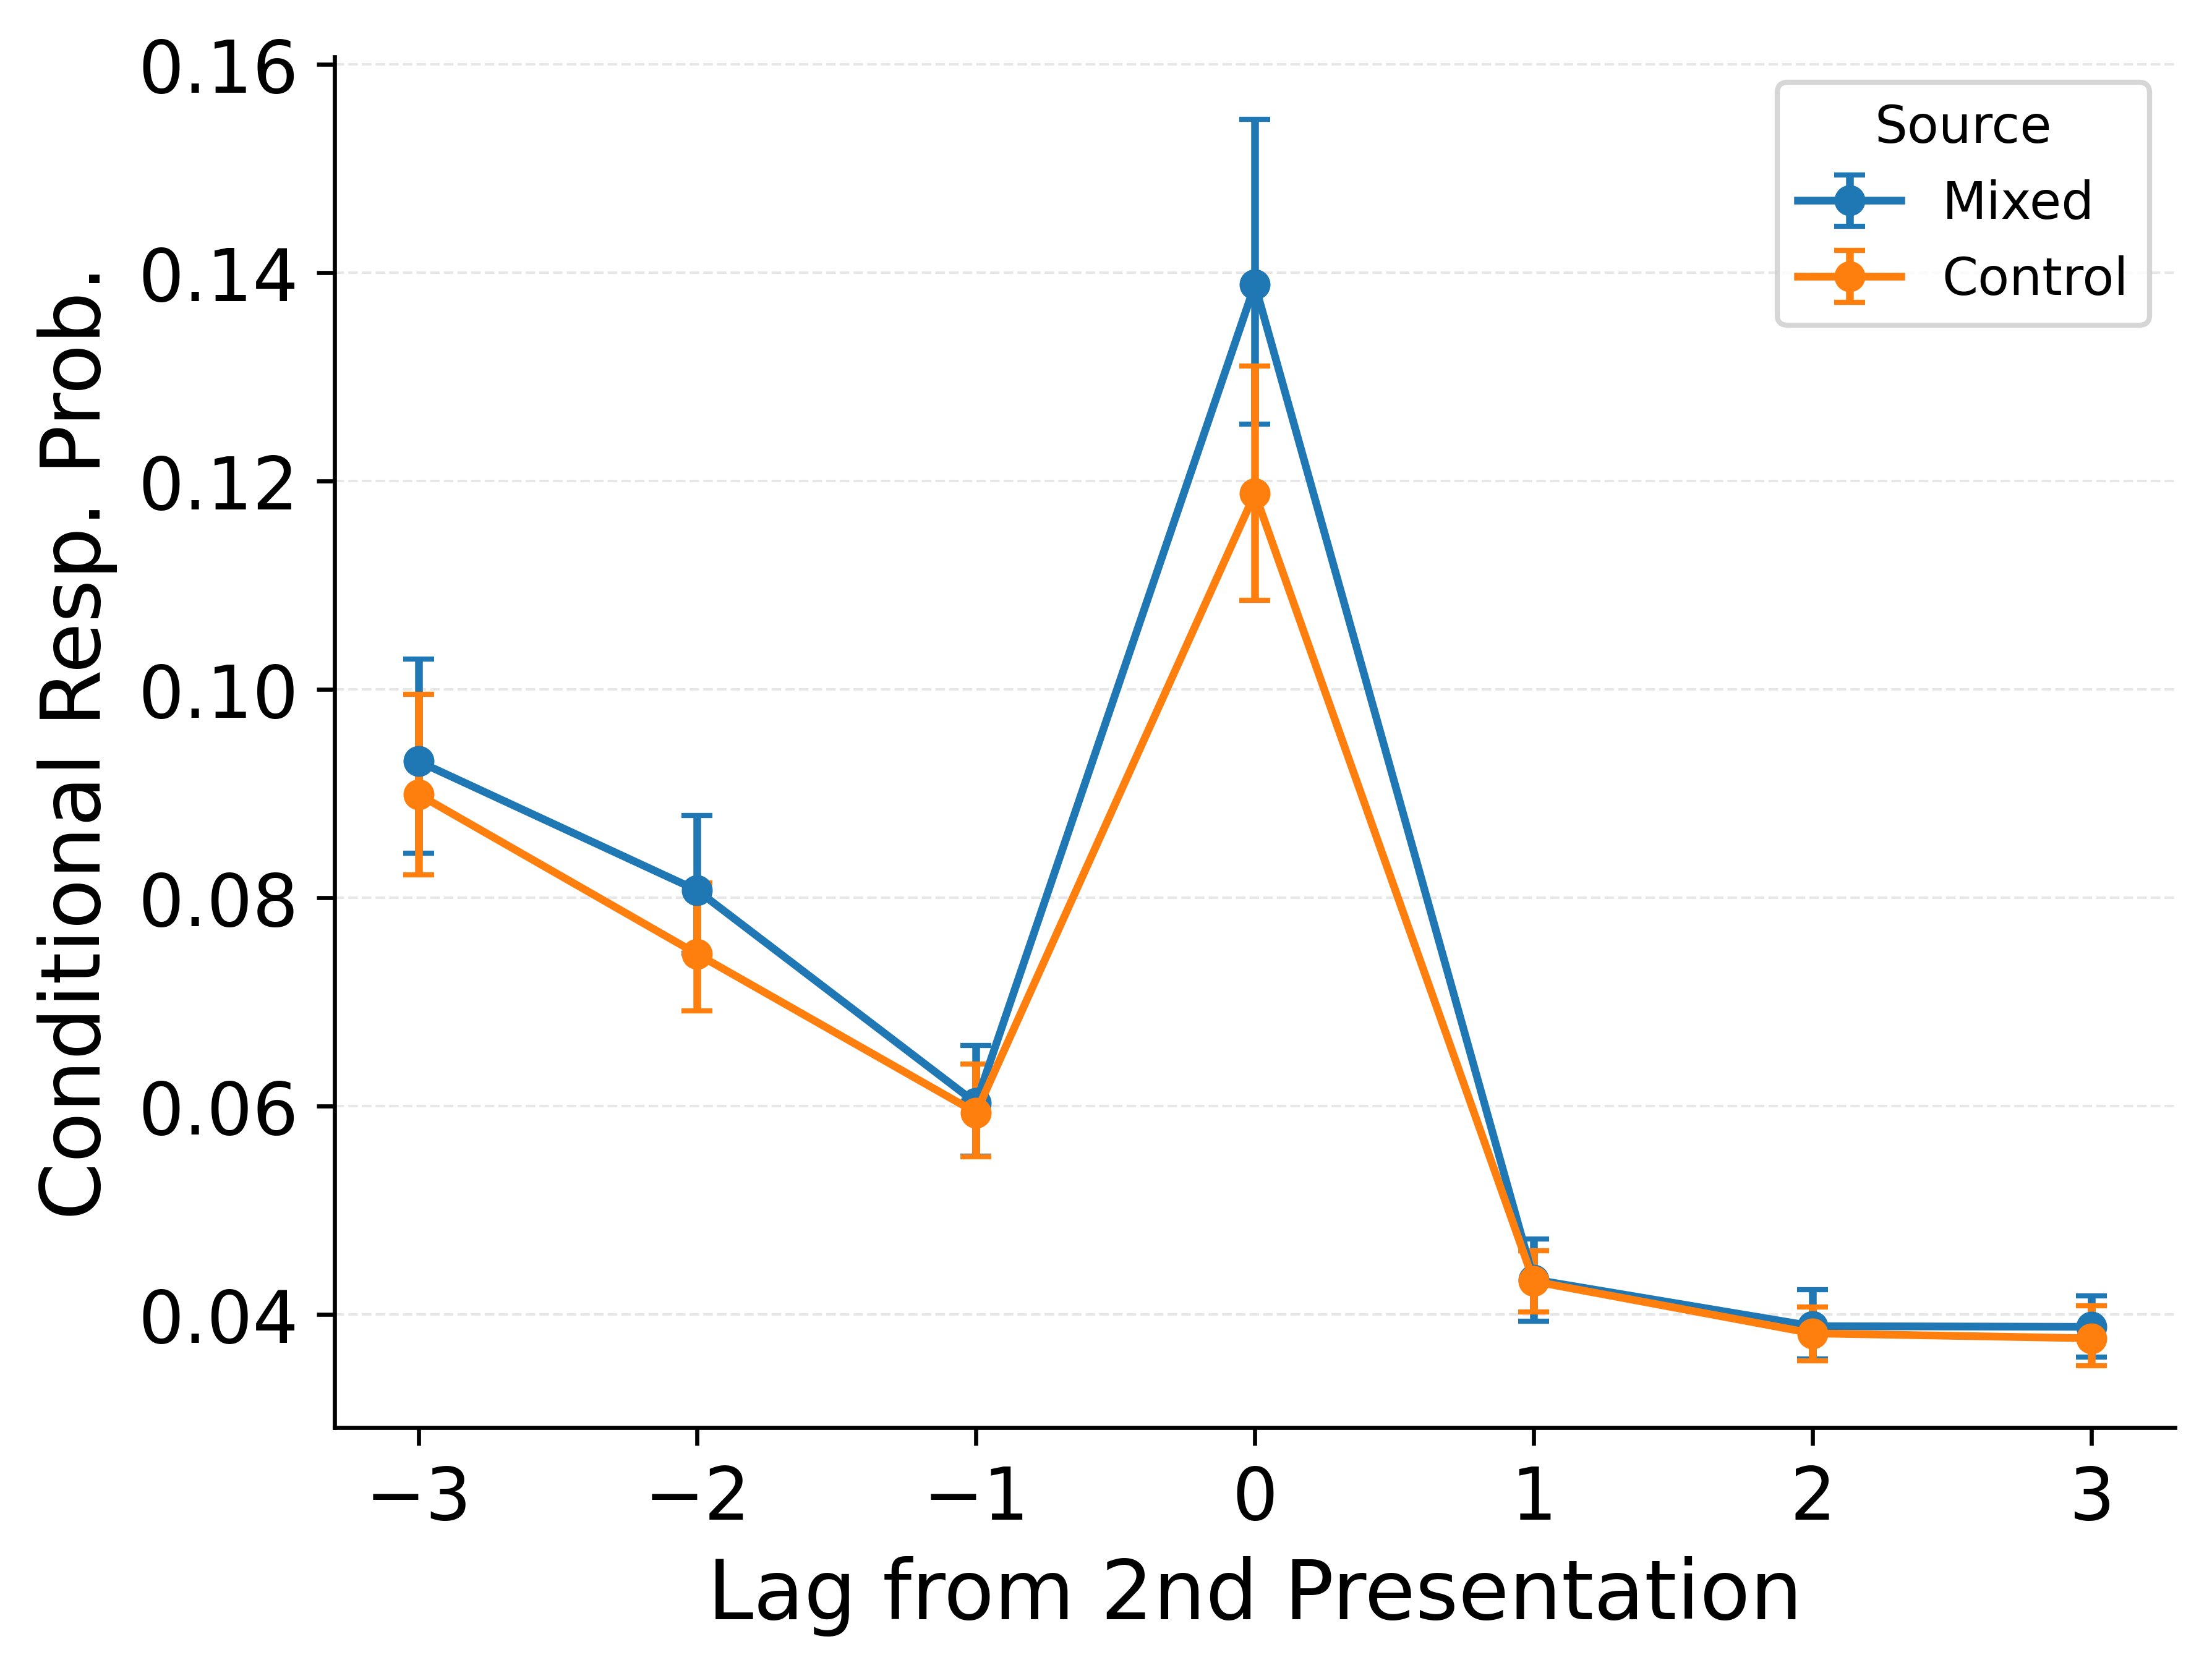
\includegraphics{../../work/thesis/figures/LohnasKahana2014_mixedvscontrolA_WeirdReinfPositionalCMR_full_best_of_3_LT4_repneighborcrp_i2j.png}\end{minipage}%
%
\begin{minipage}{0.50\linewidth}
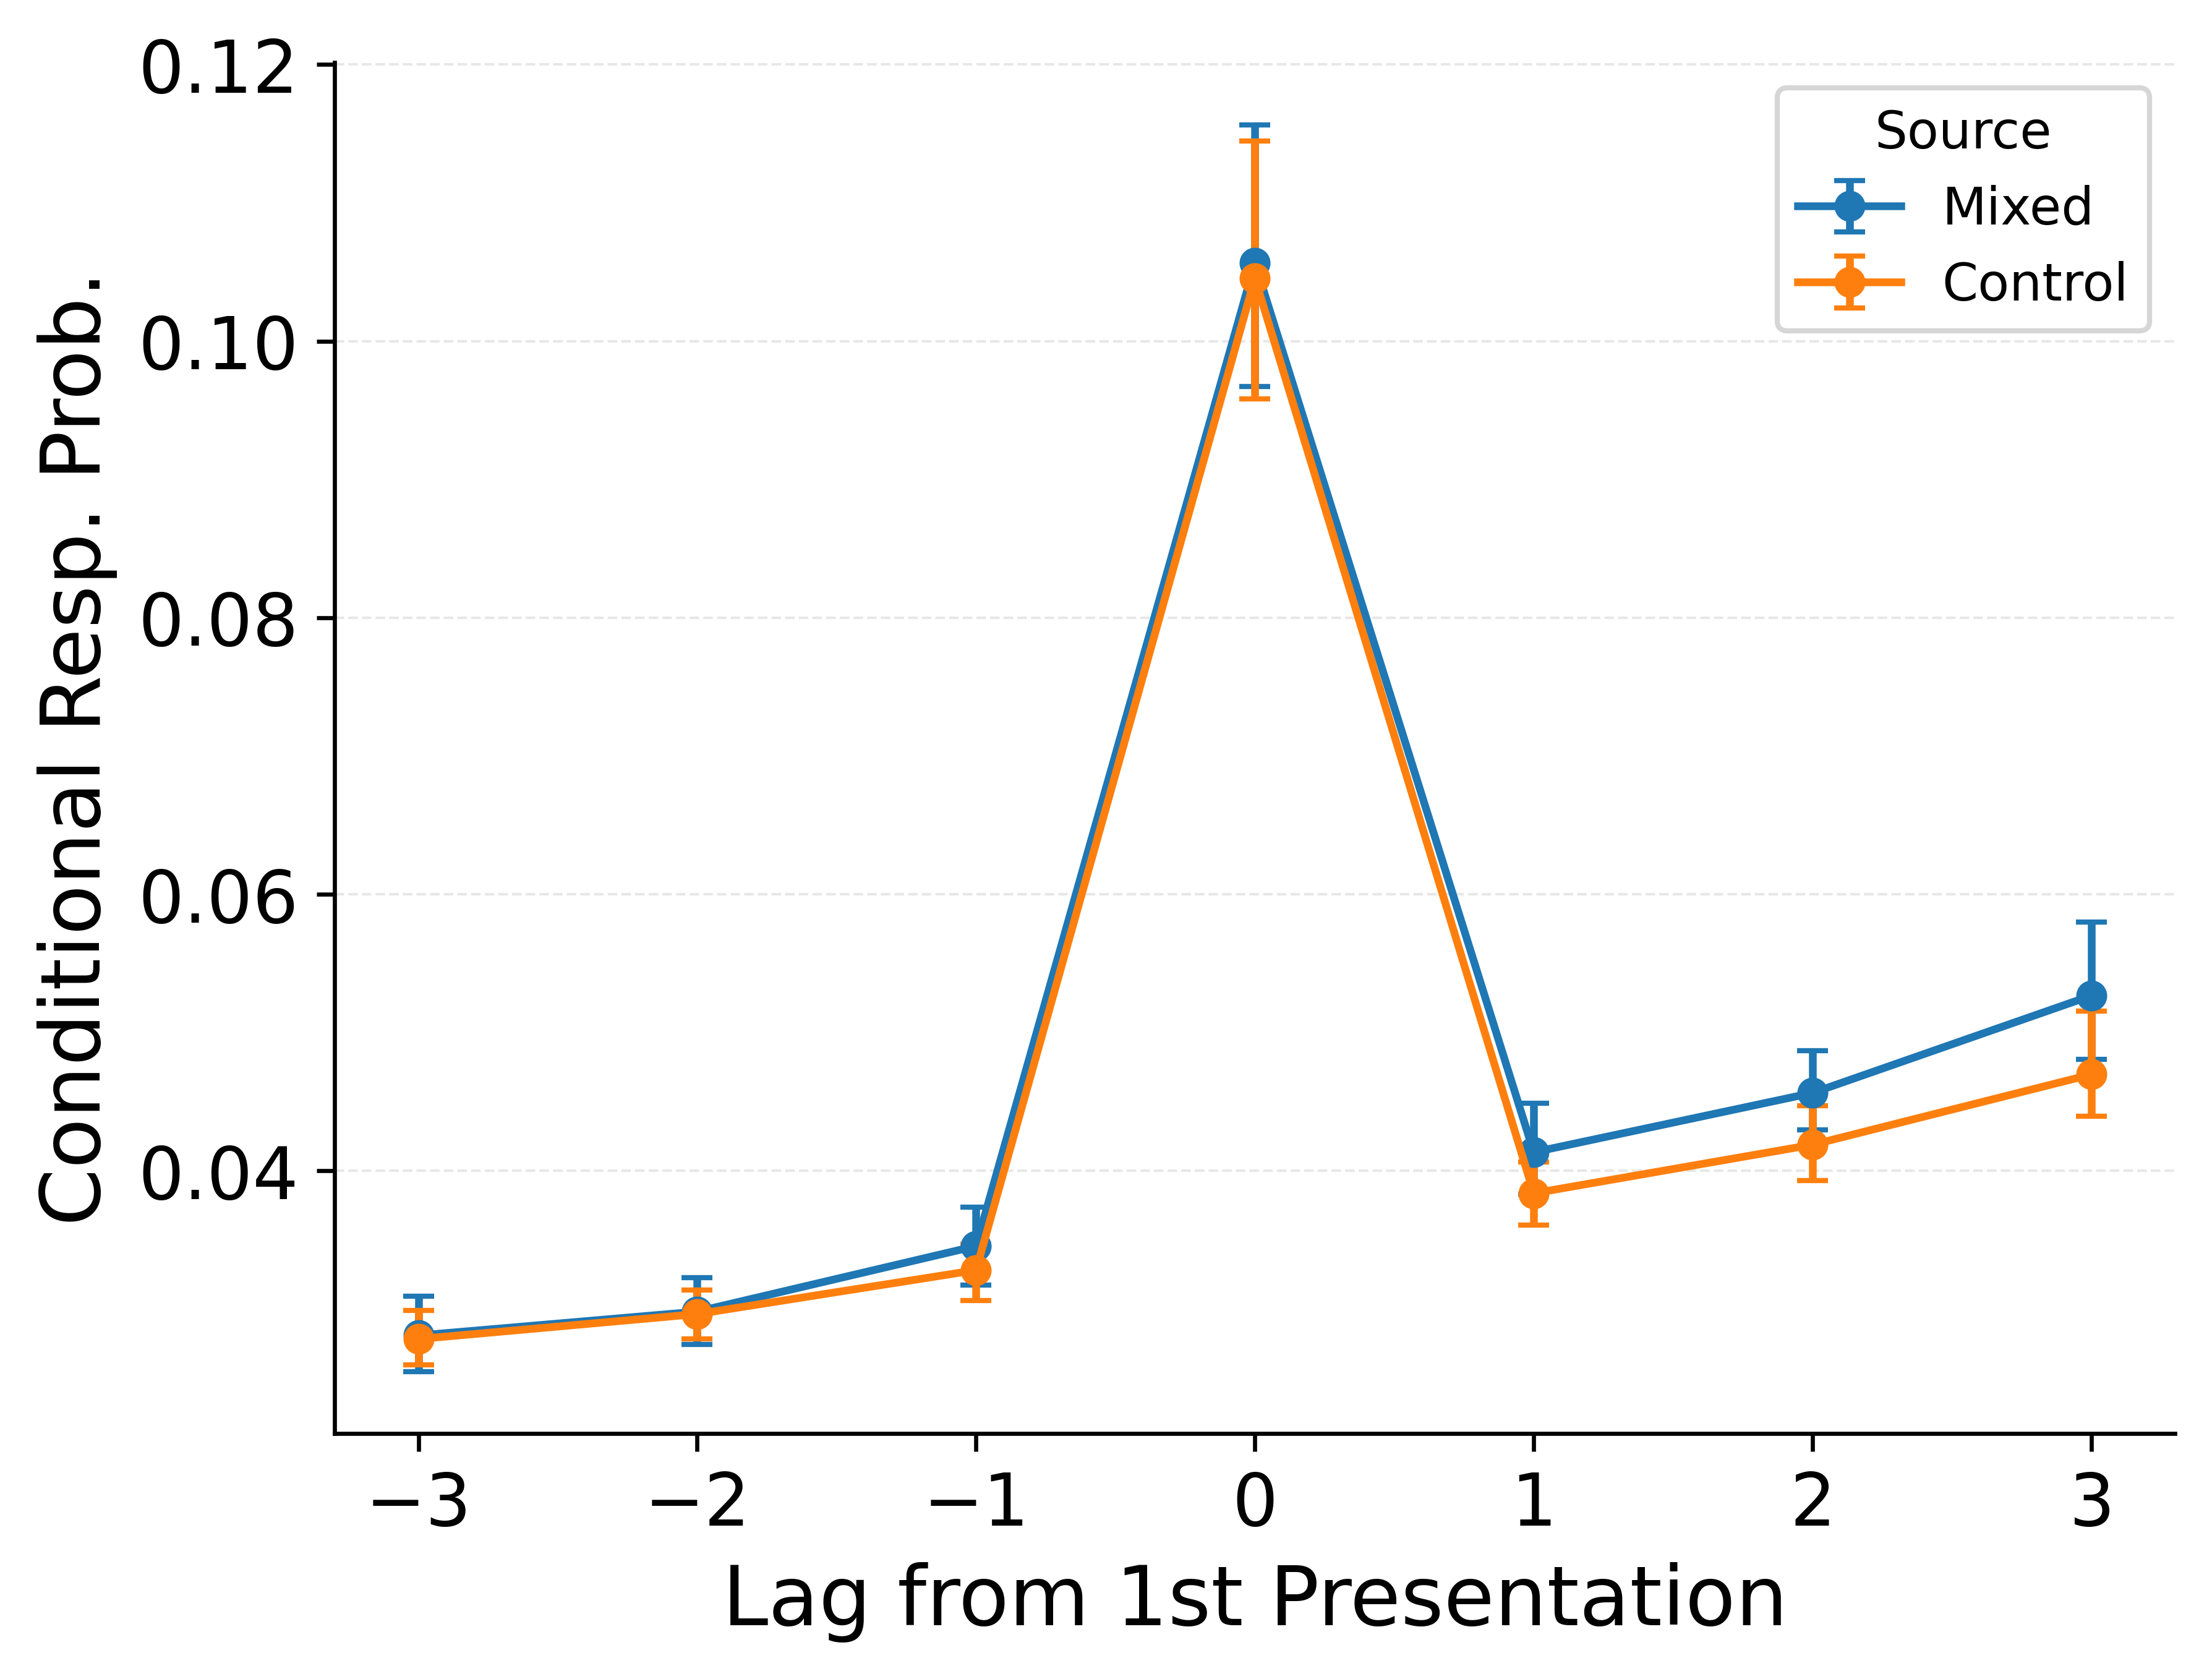
\includegraphics{../../work/thesis/figures/LohnasKahana2014_mixedvscontrolA_WeirdReinfPositionalCMR_full_best_of_3_LT4_repneighborcrp_j2i.png}\end{minipage}%

\end{figure}%

The decisive change also appears in the outgoing repetition lag-CRP. By
routing reinstatement through a single occurrence and preferentially
strengthening the first-occurrence trace, ICMR-Reinf not only avoids
balanced access but also amplifies the first-over-second separation in
mixed lists relative to the matched baseline---capturing the positive,
repetition-specific asymmetry in the data. The 2×2 comparison in
Figure~\ref{fig-reinf_rep_lag_crp} shows that where Instance-CMR
preserved only baseline-level separation, ICMR-Reinf produces the
boosted separation observed empirically.

\begin{figure}

\caption{\label{fig-reinf_rep_lag_crp}Repetition lag-CRP (outgoing):
data vs ICMR-Reinf. Top: mixed lists (left) and matched-control baseline
(right) from Lohnas and Kahana
(\citeproc{ref-lohnas2014retrieved}{2014}). Bottom: ICMR-Reinf
simulations scored identically. In mixed lists, the +1 bin and nearby
lags show a larger first-over-second separation than in
baseline---matching the data's boosted separation. Balanced-access
(blending) is absent.}

\begin{minipage}{0.50\linewidth}
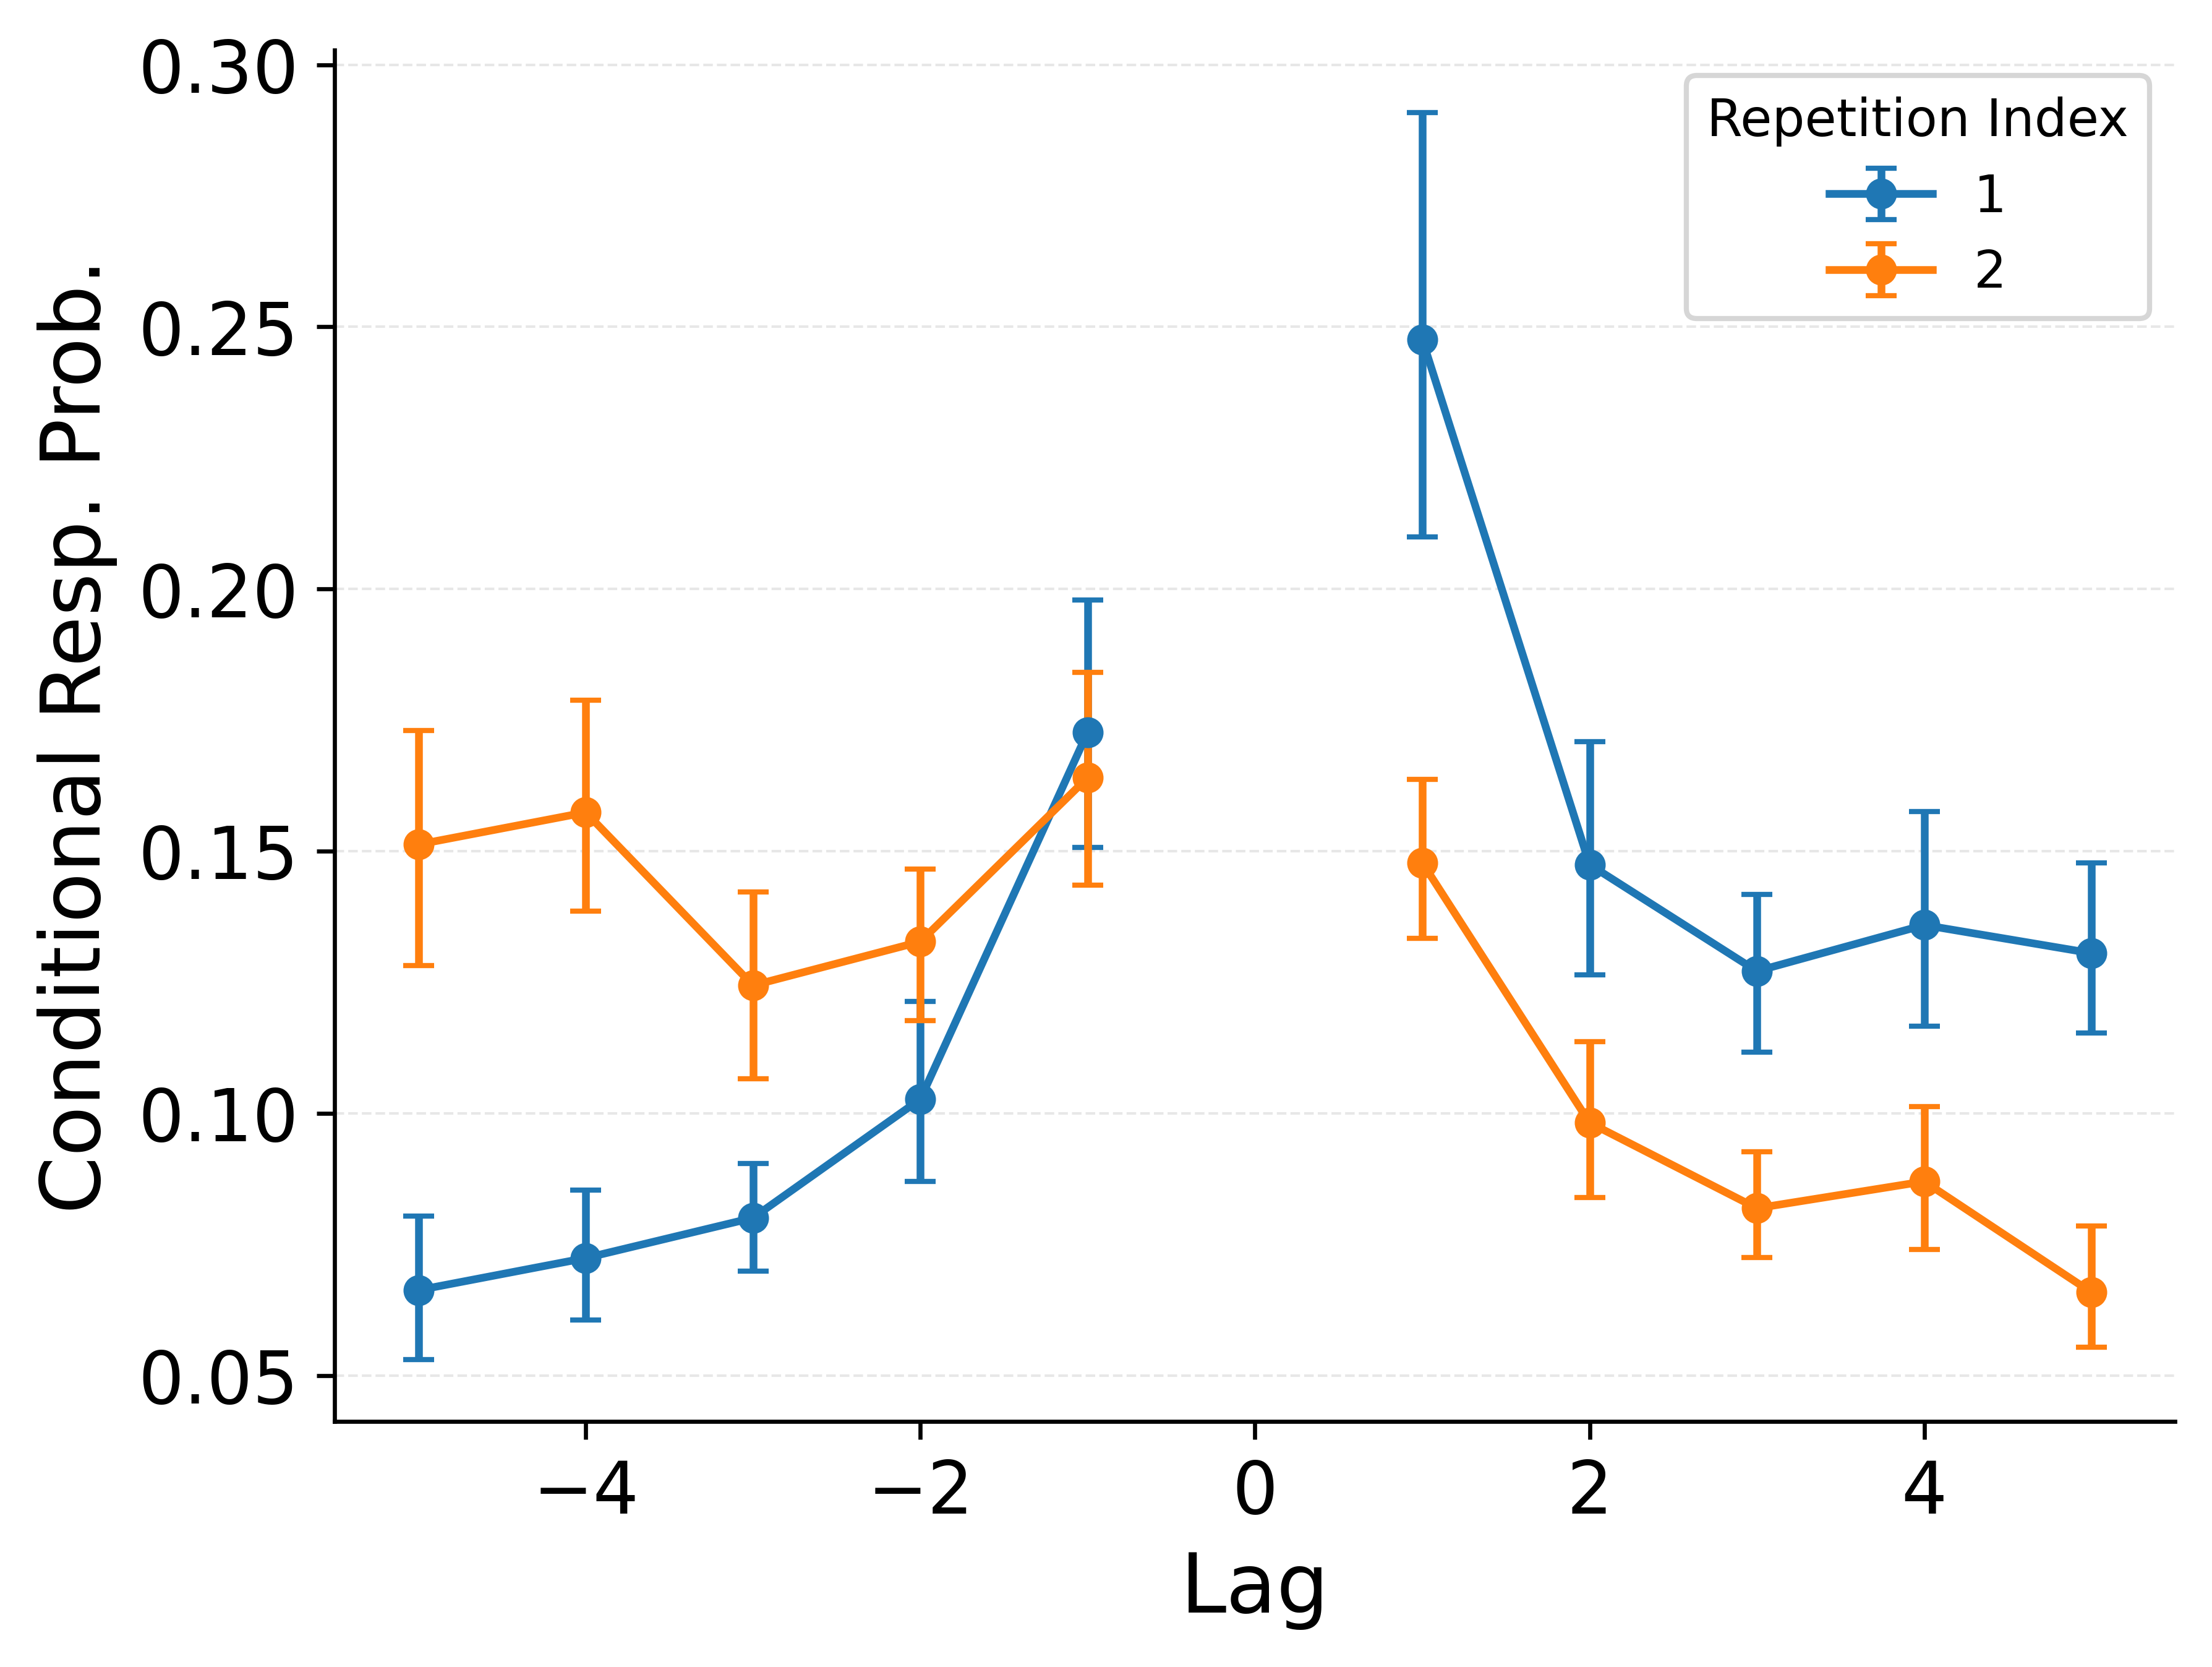
\includegraphics{../../work/thesis/figures/RepeatedRecallsLohnasKahana2014_mixed_data_full_best_of_3_LT34_rep_crp.png}\end{minipage}%
%
\begin{minipage}{0.50\linewidth}
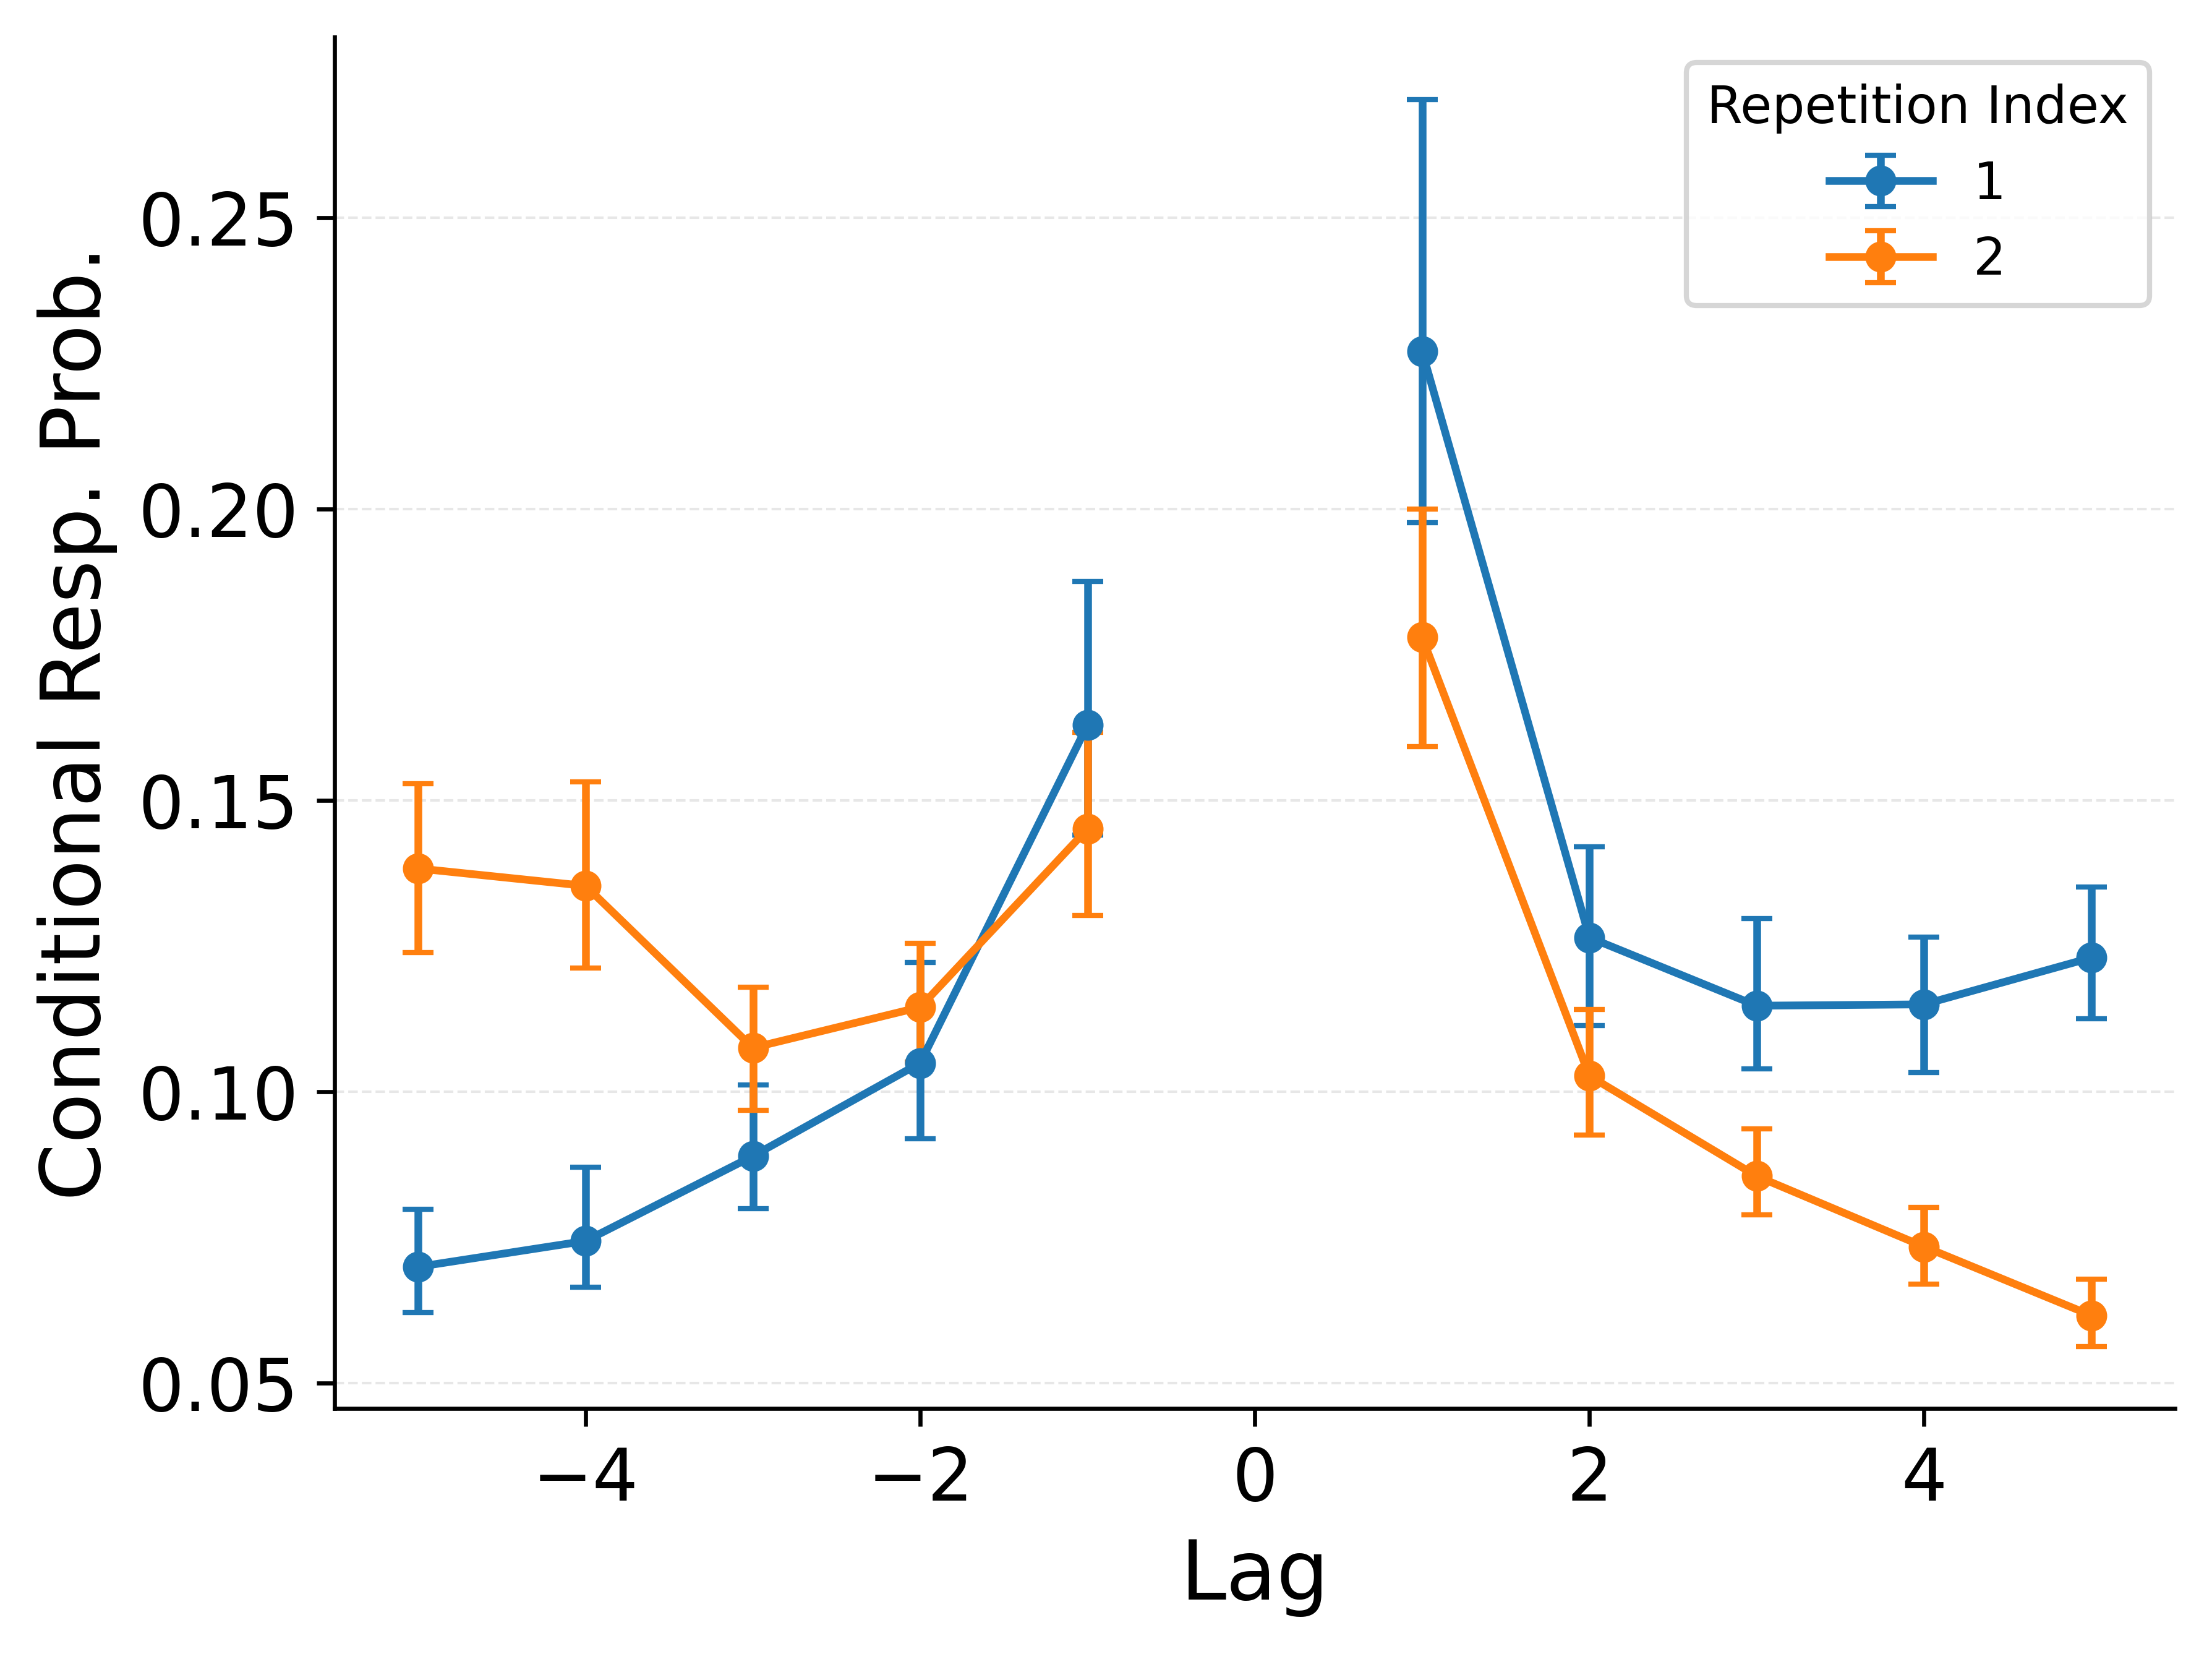
\includegraphics{../../work/thesis/figures/RepeatedRecallsLohnasKahana2014_control_data_full_best_of_3_LT34_rep_crp.png}\end{minipage}%
\newline
\begin{minipage}{0.50\linewidth}
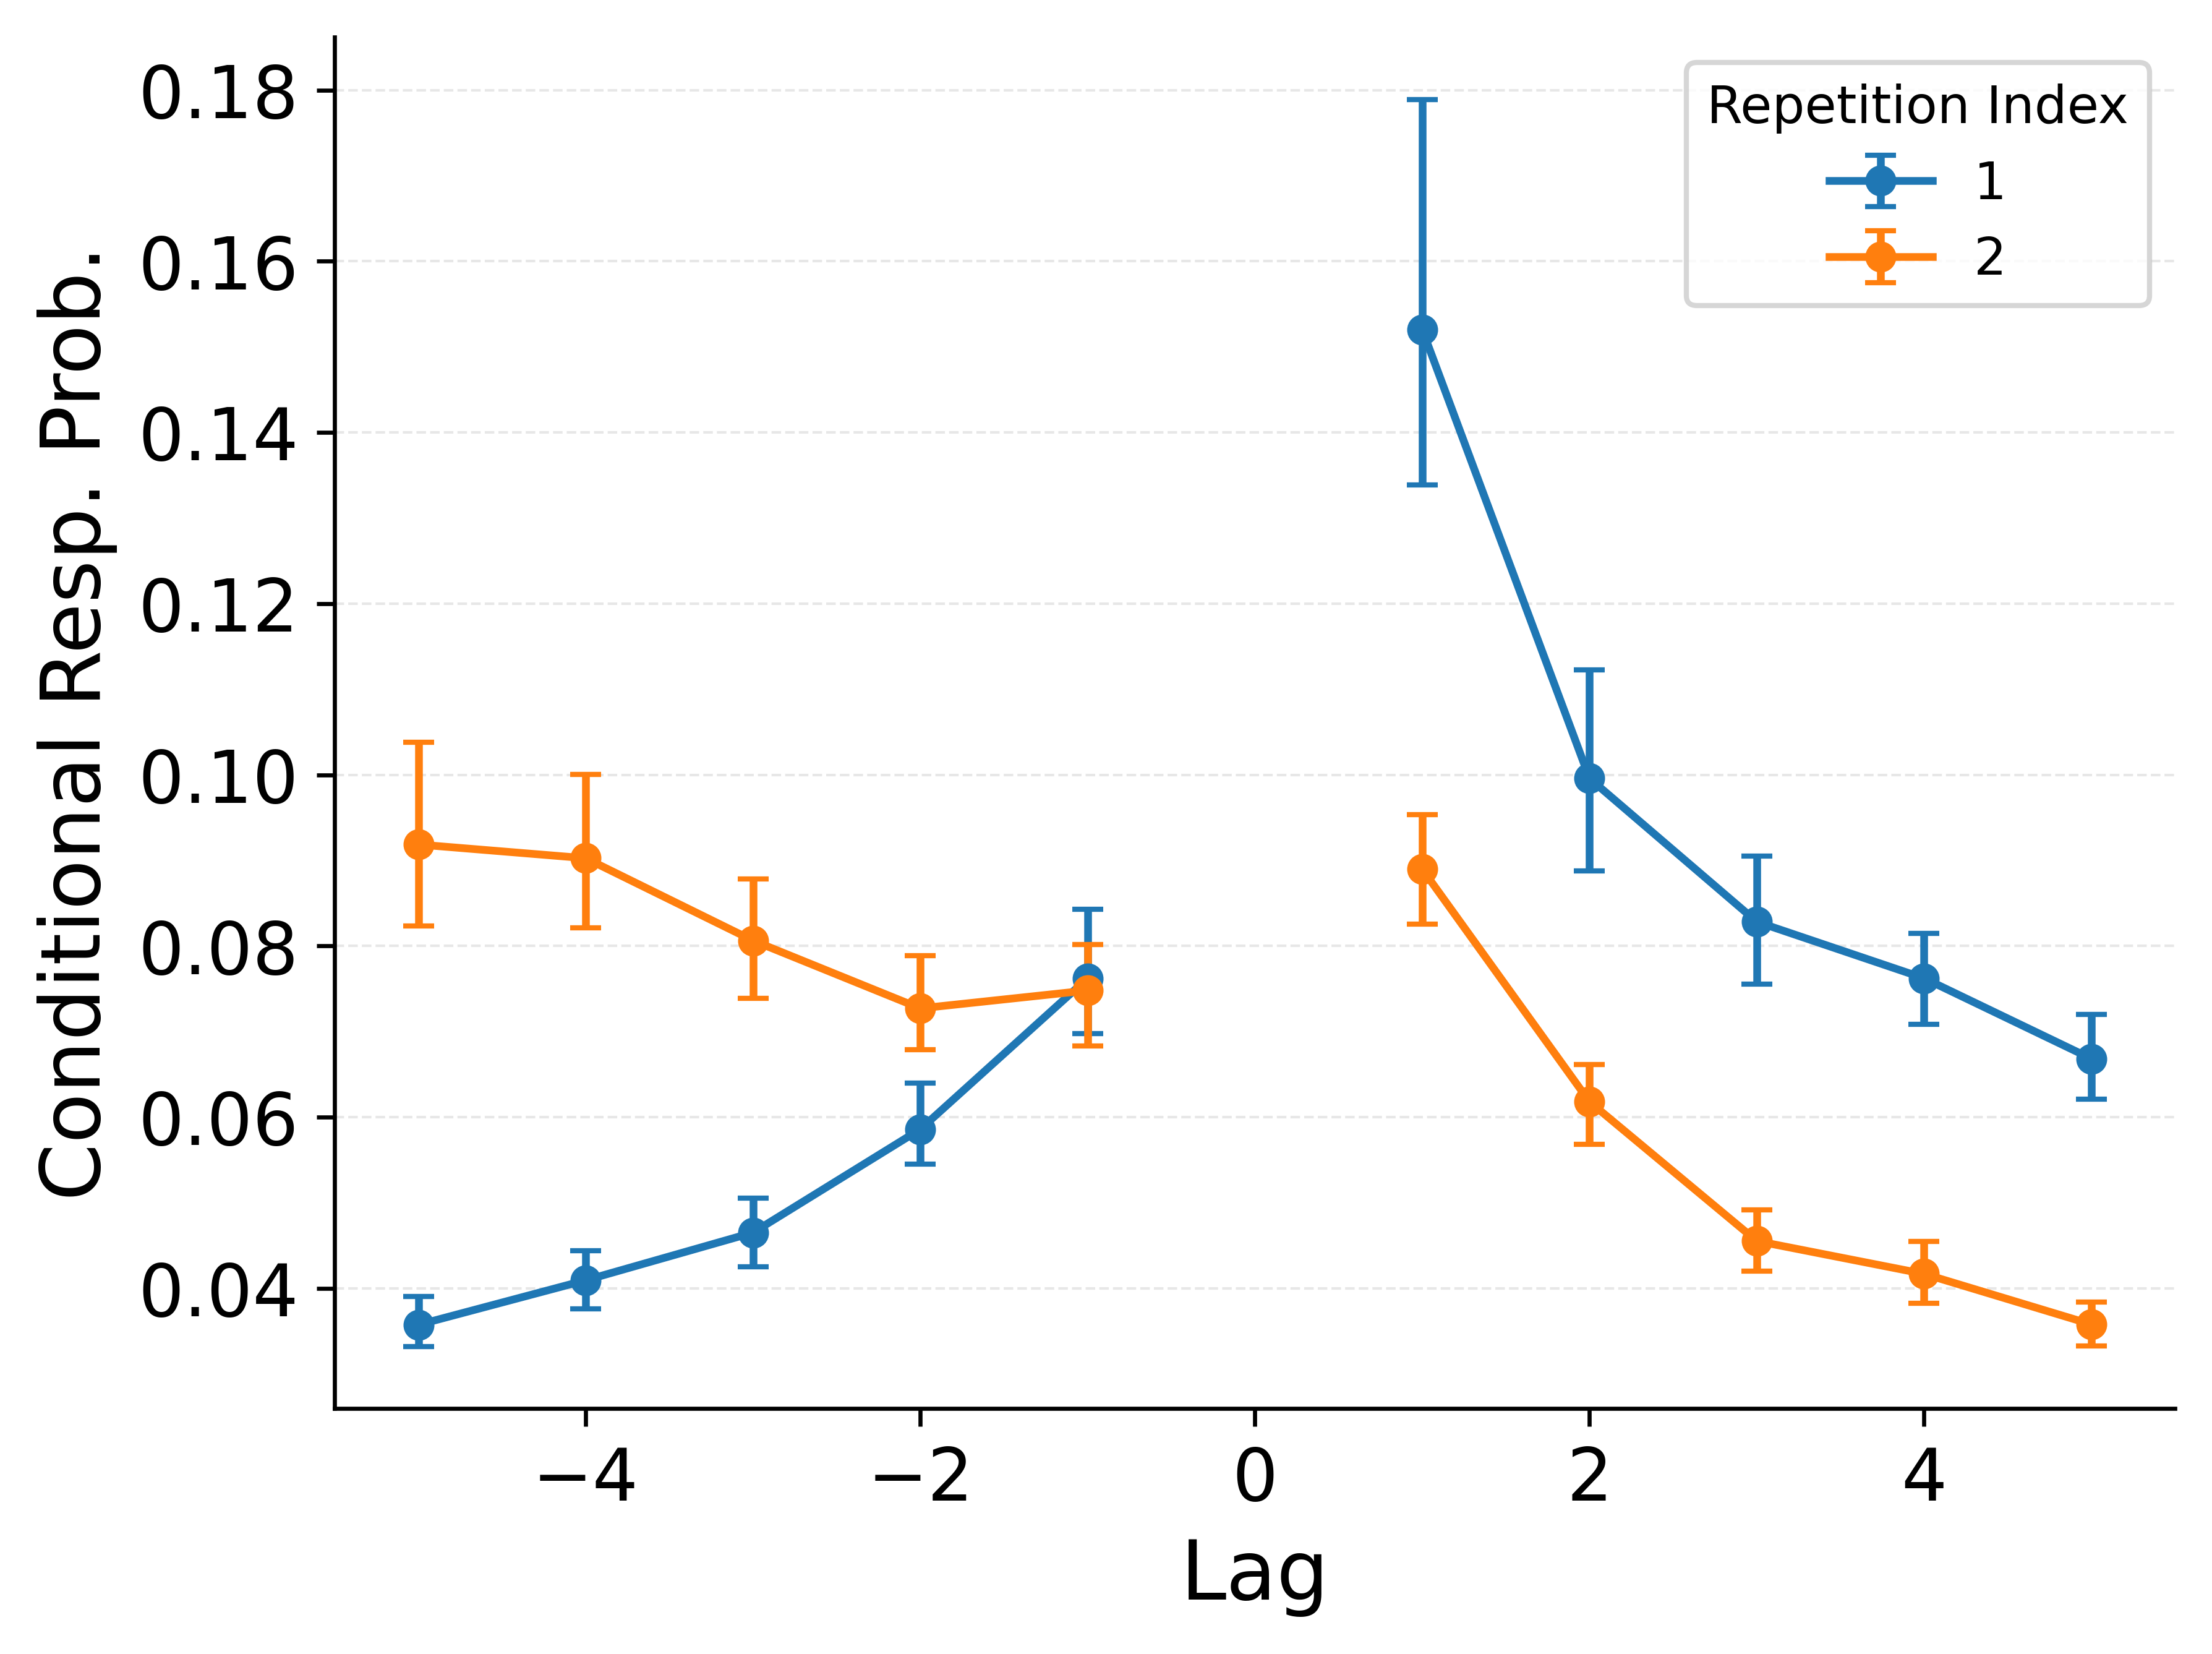
\includegraphics{../../work/thesis/figures/LohnasKahana2014_mixed_WeirdReinfPositionalCMR_full_best_of_3_LT4_rep_crp.png}\end{minipage}%
%
\begin{minipage}{0.50\linewidth}
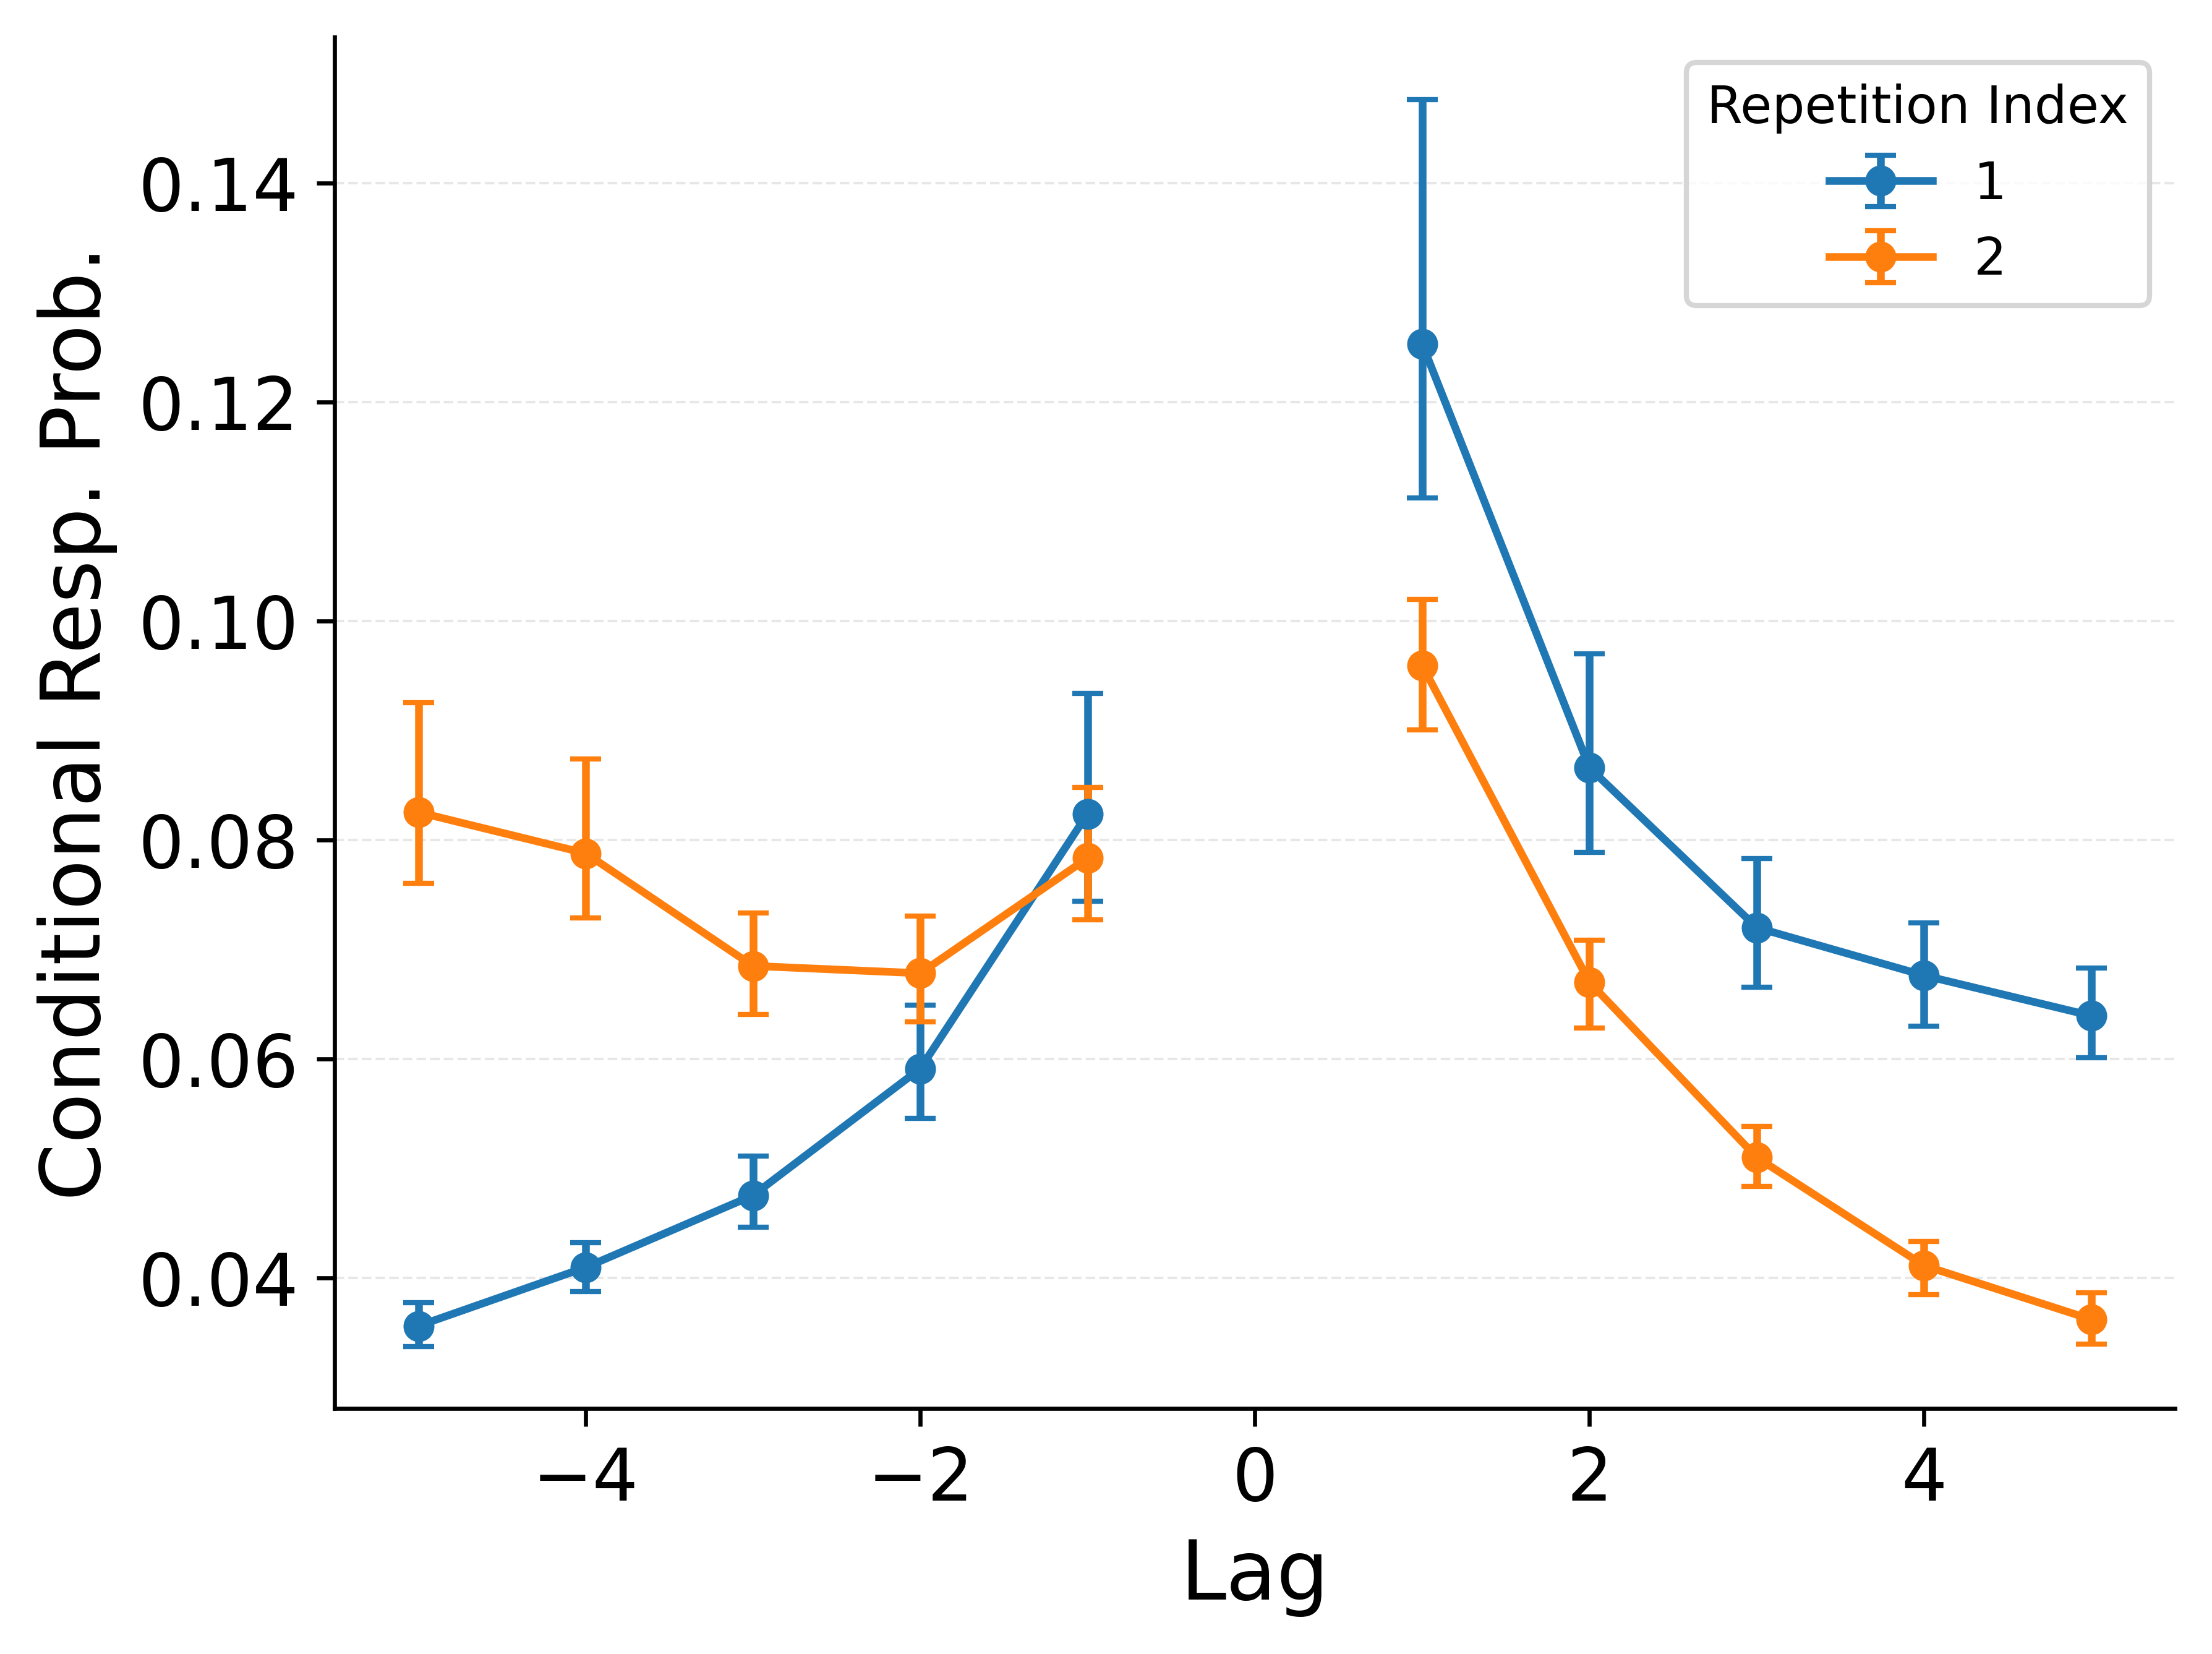
\includegraphics{../../work/thesis/figures/LohnasKahana2014_control_WeirdReinfPositionalCMR_full_best_of_3_LT4_rep_crp.png}\end{minipage}%

\end{figure}%

For the incoming/backward repetition lag-CRP
(Figure~\ref{fig-reinf_back_rep_crp}), reinforcement increases arrivals
from the first occurrence's backward neighbor relative to the second,
strengthening the first-over-second preference beyond Instance-CMR and
moving the model toward the empirical pattern. Because this variant
largely reflects how the search state approached the repeater, the
outgoing mixed--minus--baseline contrast remains the cleanest probe of
repetition-specific reinstatement, and that is where ICMR-Reinf shows
its clearest advantage.

\begin{figure}

\caption{\label{fig-reinf_back_rep_crp}Repetition lag-CRP
(incoming/backward). Top: mixed lists (left) and matched-control
baseline (right) from Lohnas and Kahana
(\citeproc{ref-lohnas2014retrieved}{2014}). Bottom: ICMR-Reinf
simulations scored identically. In mixed lists, the +1 bin and nearby
lags show a larger first-over-second separation than in
baseline---matching the data's boosted separation. Balanced-access
(blending) is absent.}

\begin{minipage}{0.50\linewidth}
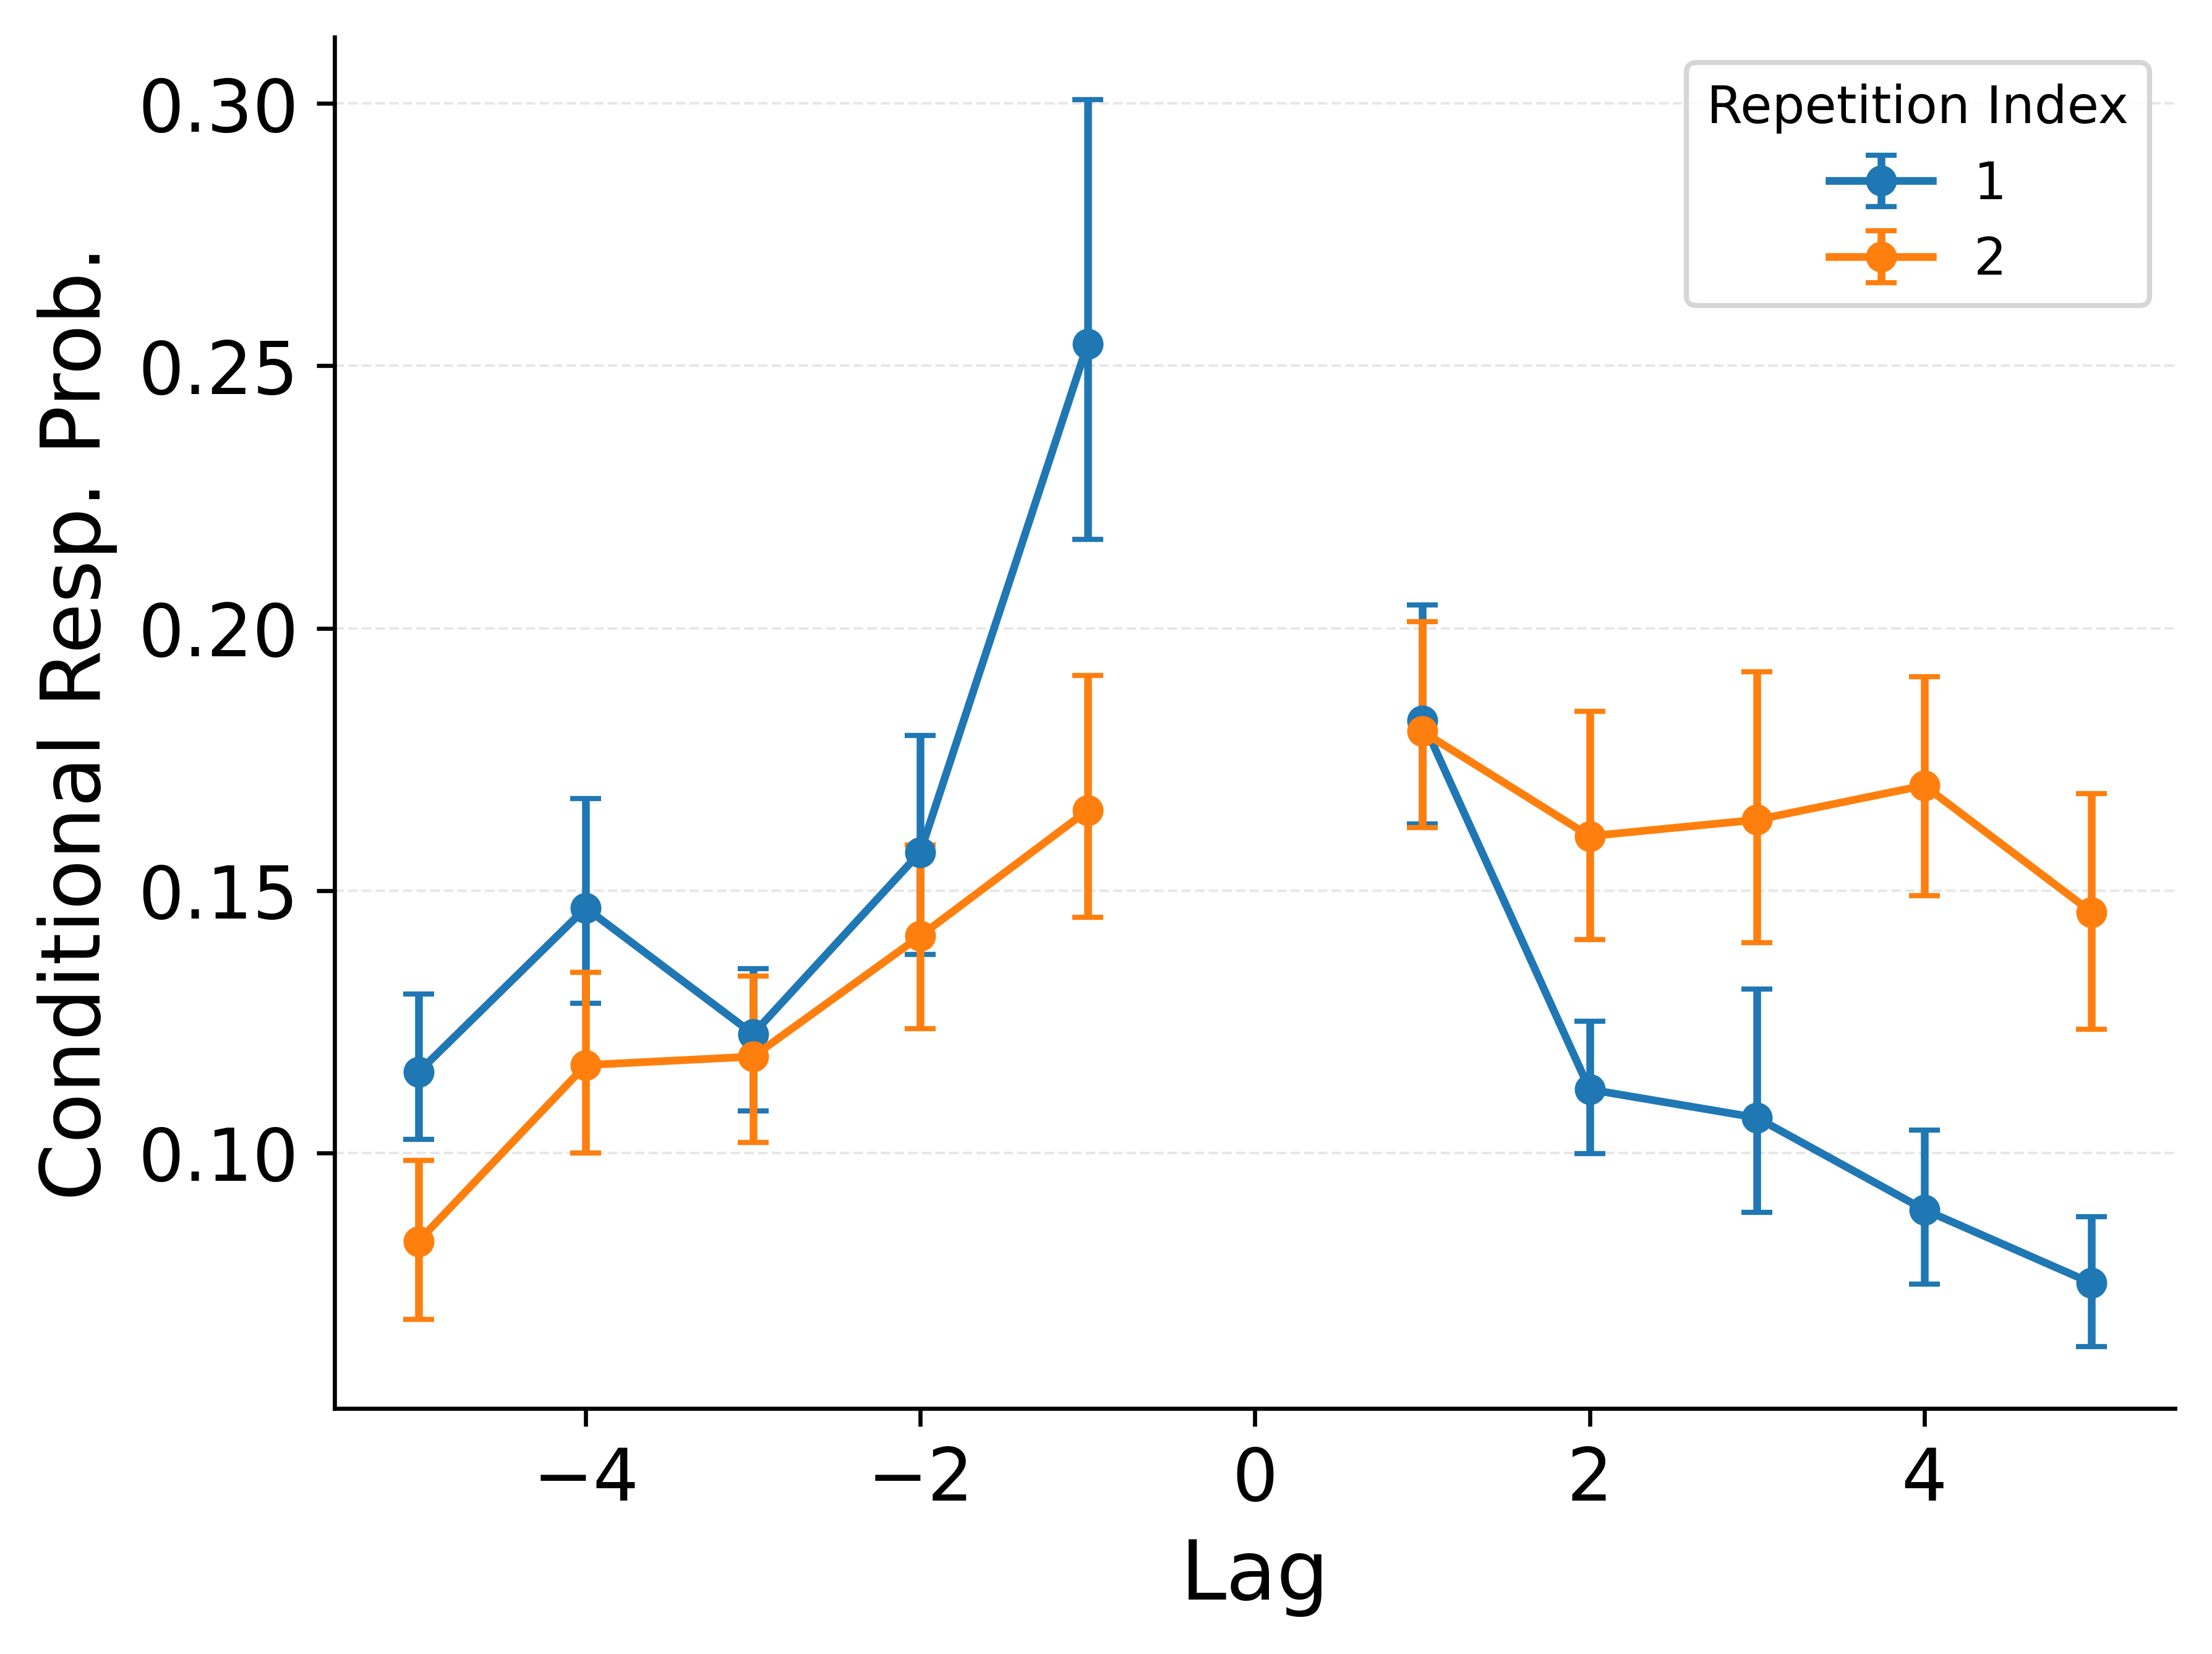
\includegraphics{../../work/thesis/figures/RepeatedRecallsLohnasKahana2014_mixed_data_full_best_of_3_LT34_back_rep_crp.png}\end{minipage}%
%
\begin{minipage}{0.50\linewidth}
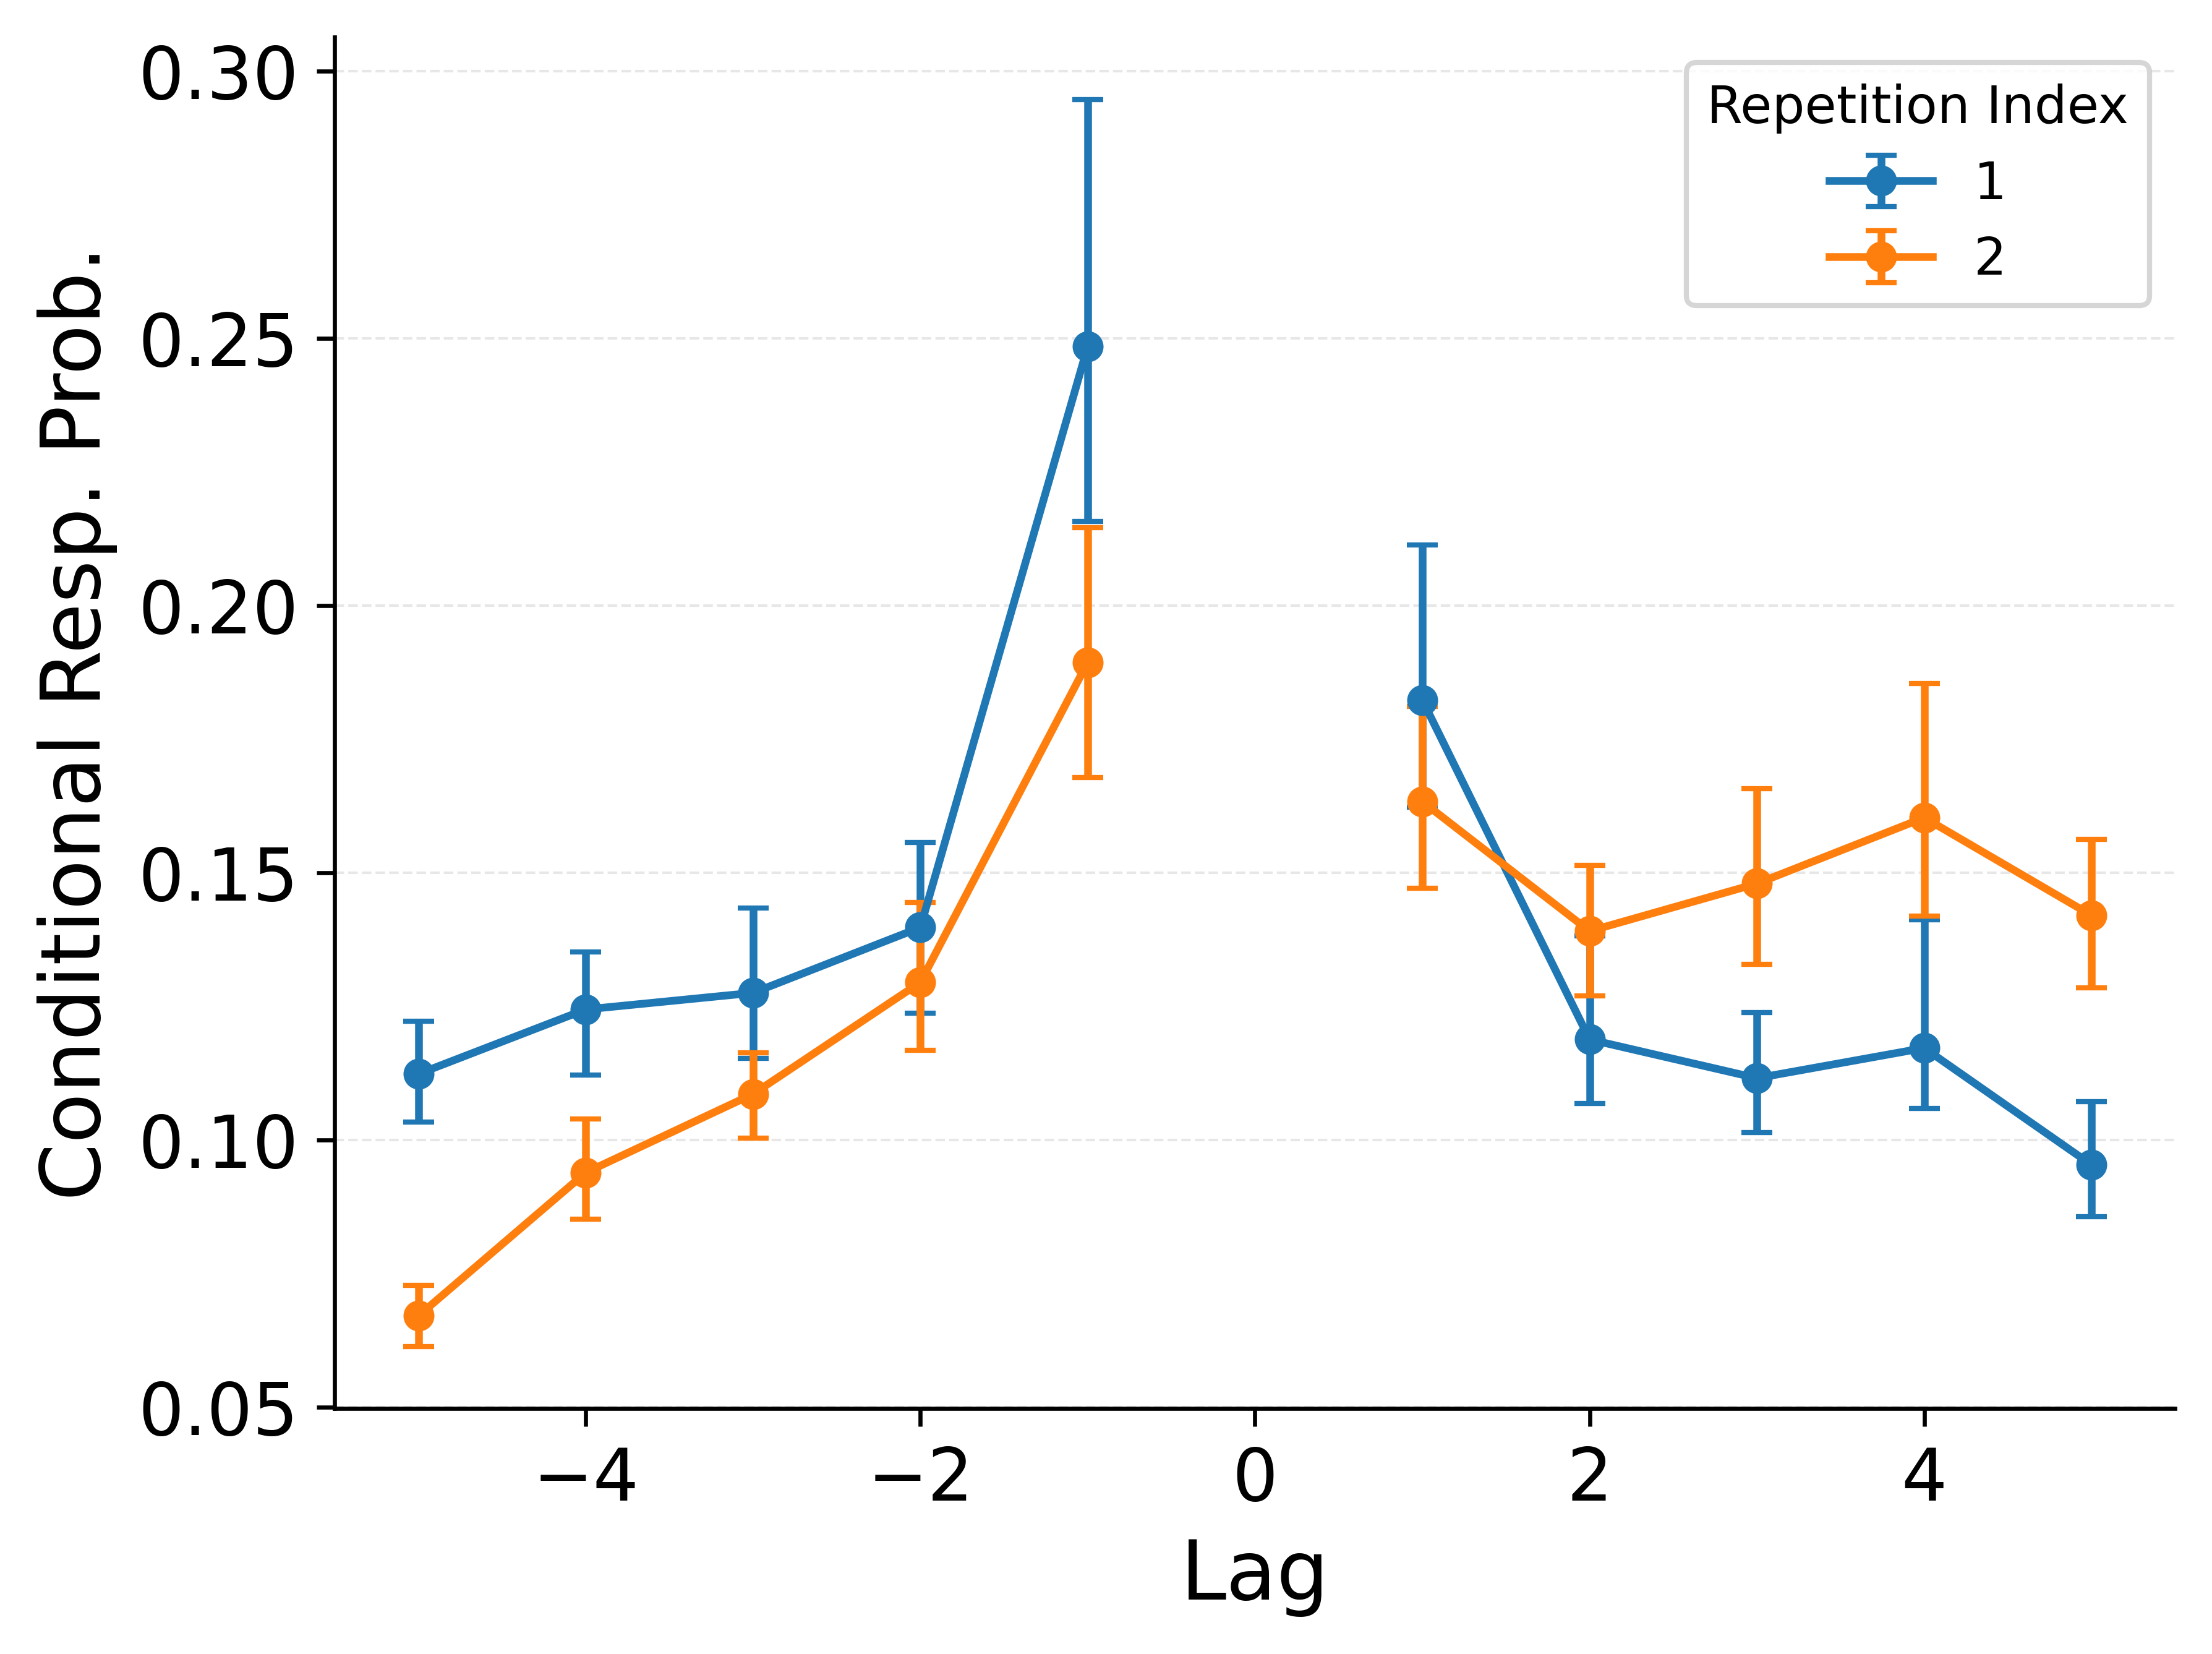
\includegraphics{../../work/thesis/figures/RepeatedRecallsLohnasKahana2014_control_data_full_best_of_3_LT34_back_rep_crp.png}\end{minipage}%
\newline
\begin{minipage}{0.50\linewidth}
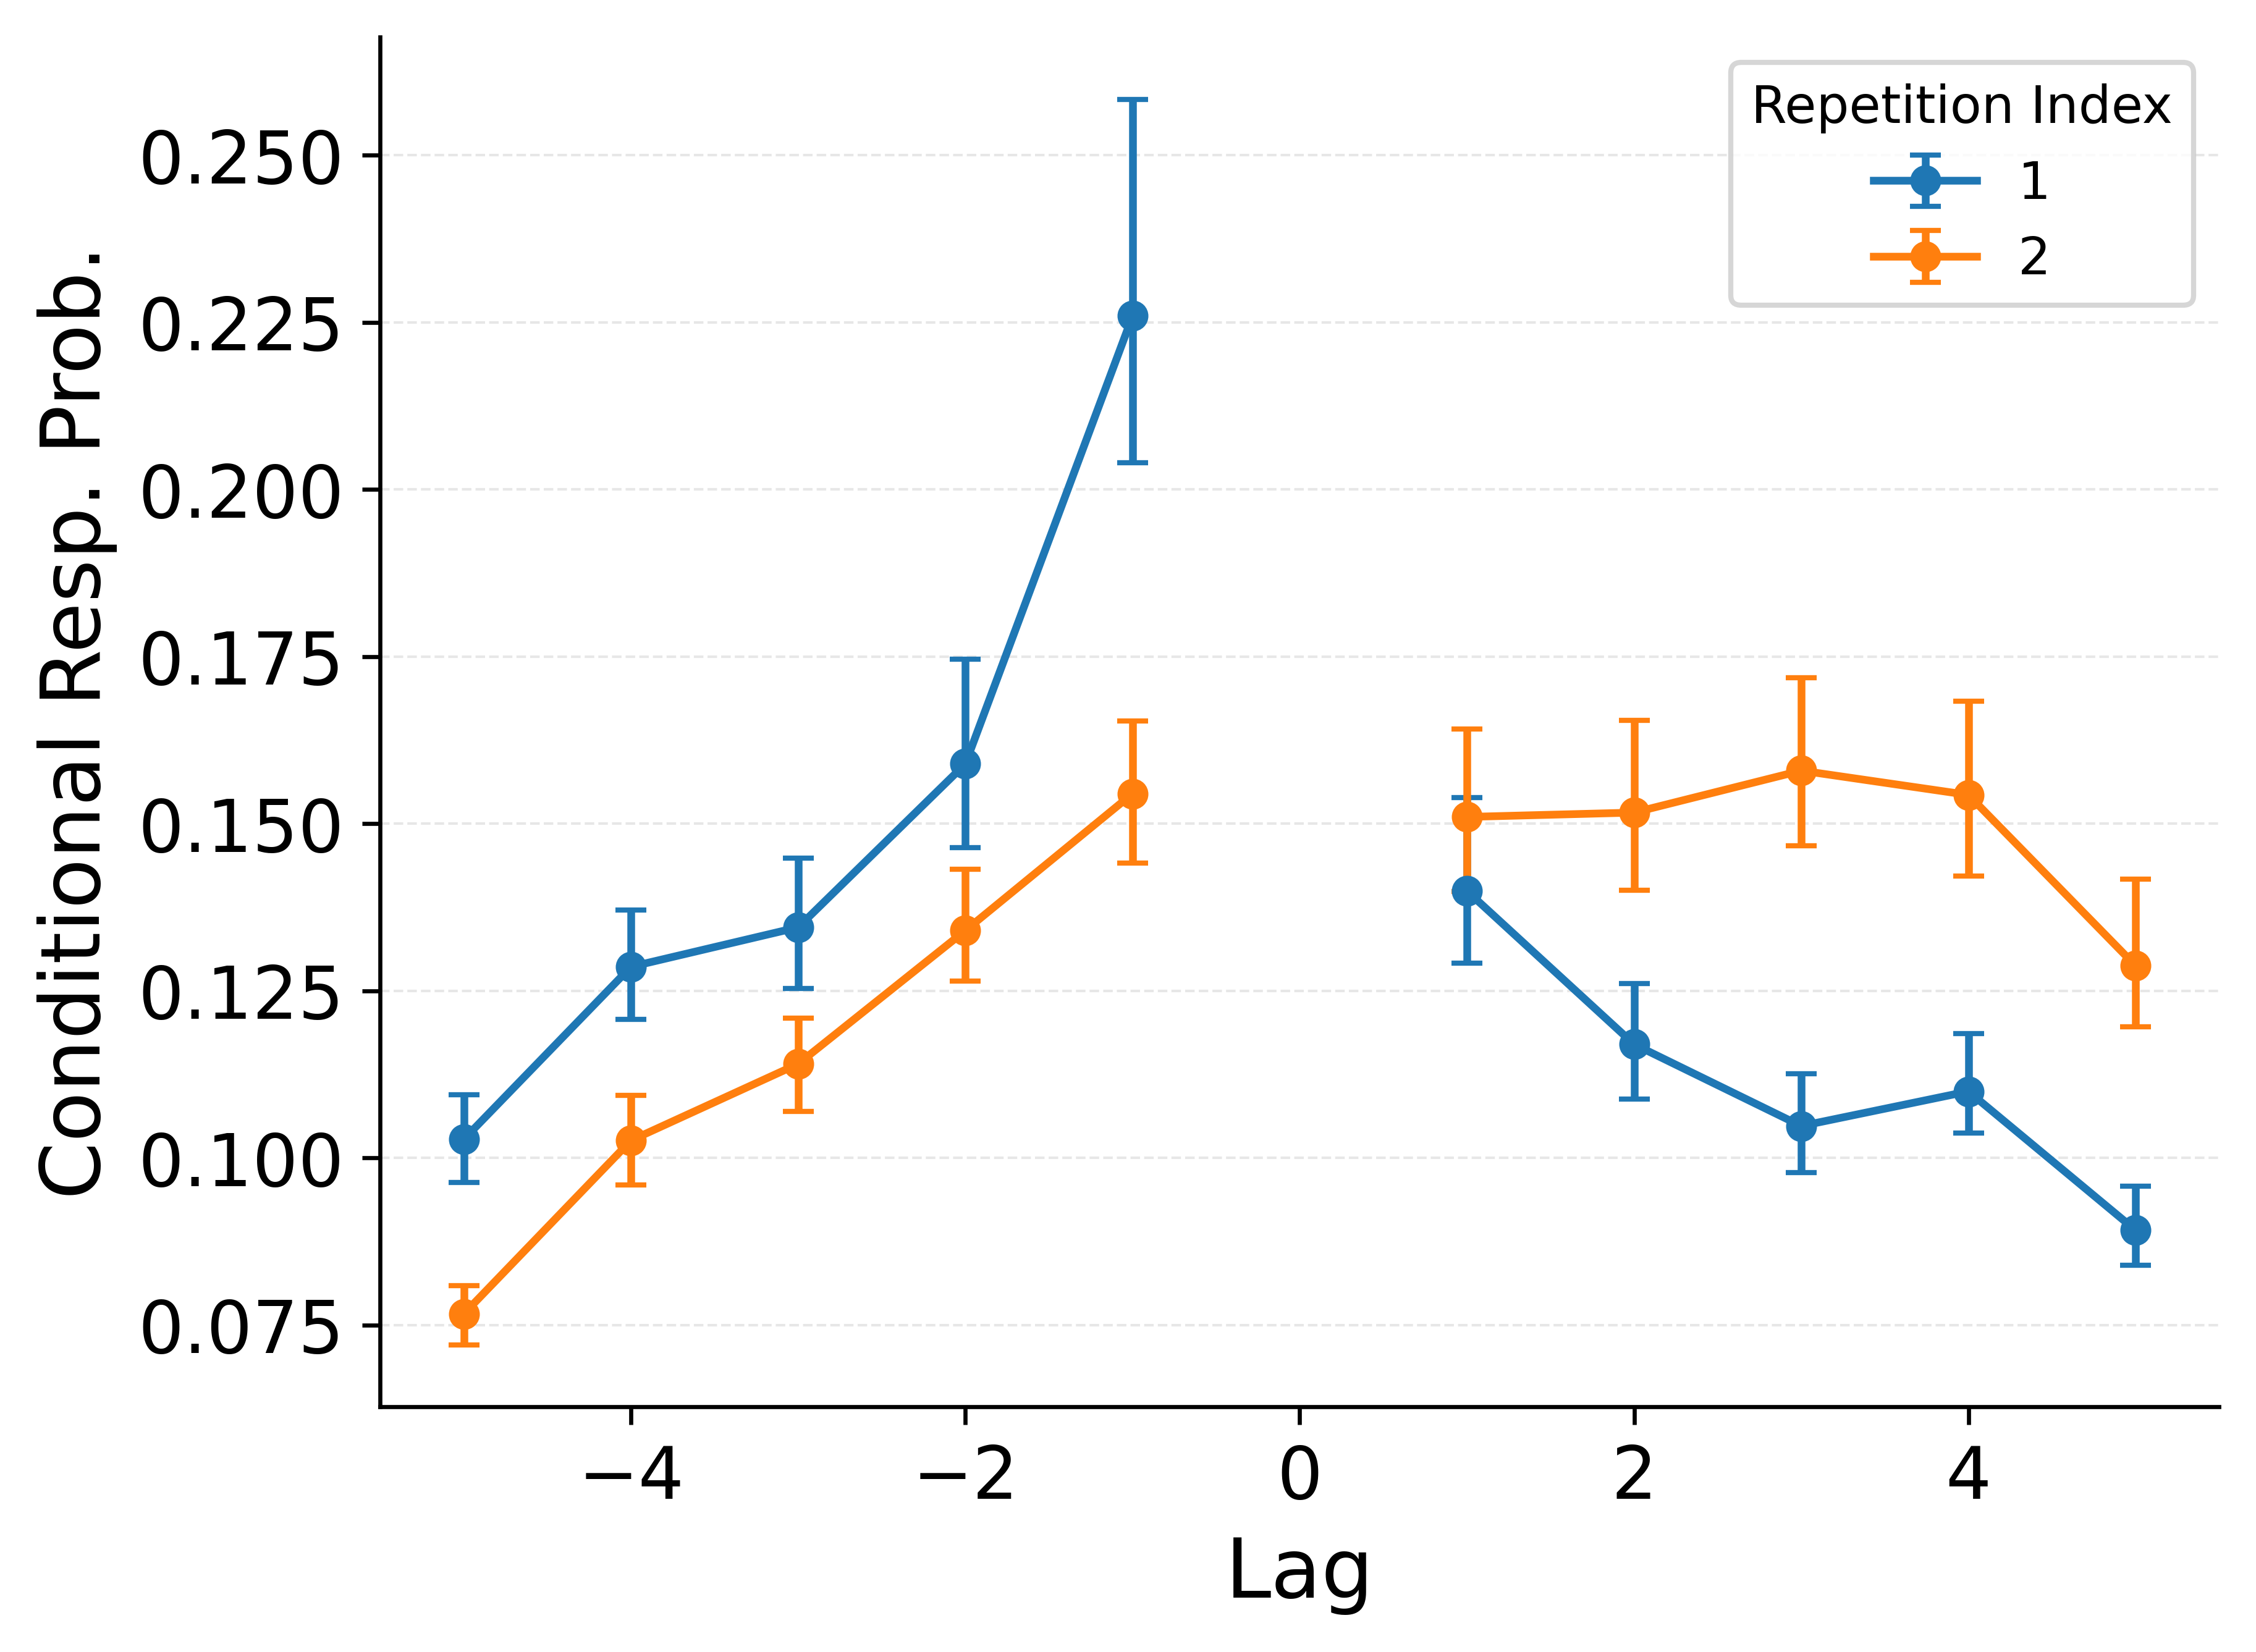
\includegraphics{../../work/thesis/figures/LohnasKahana2014_mixed_WeirdReinfPositionalCMR_full_best_of_3_LT34_back_rep_crp.png}\end{minipage}%
%
\begin{minipage}{0.50\linewidth}
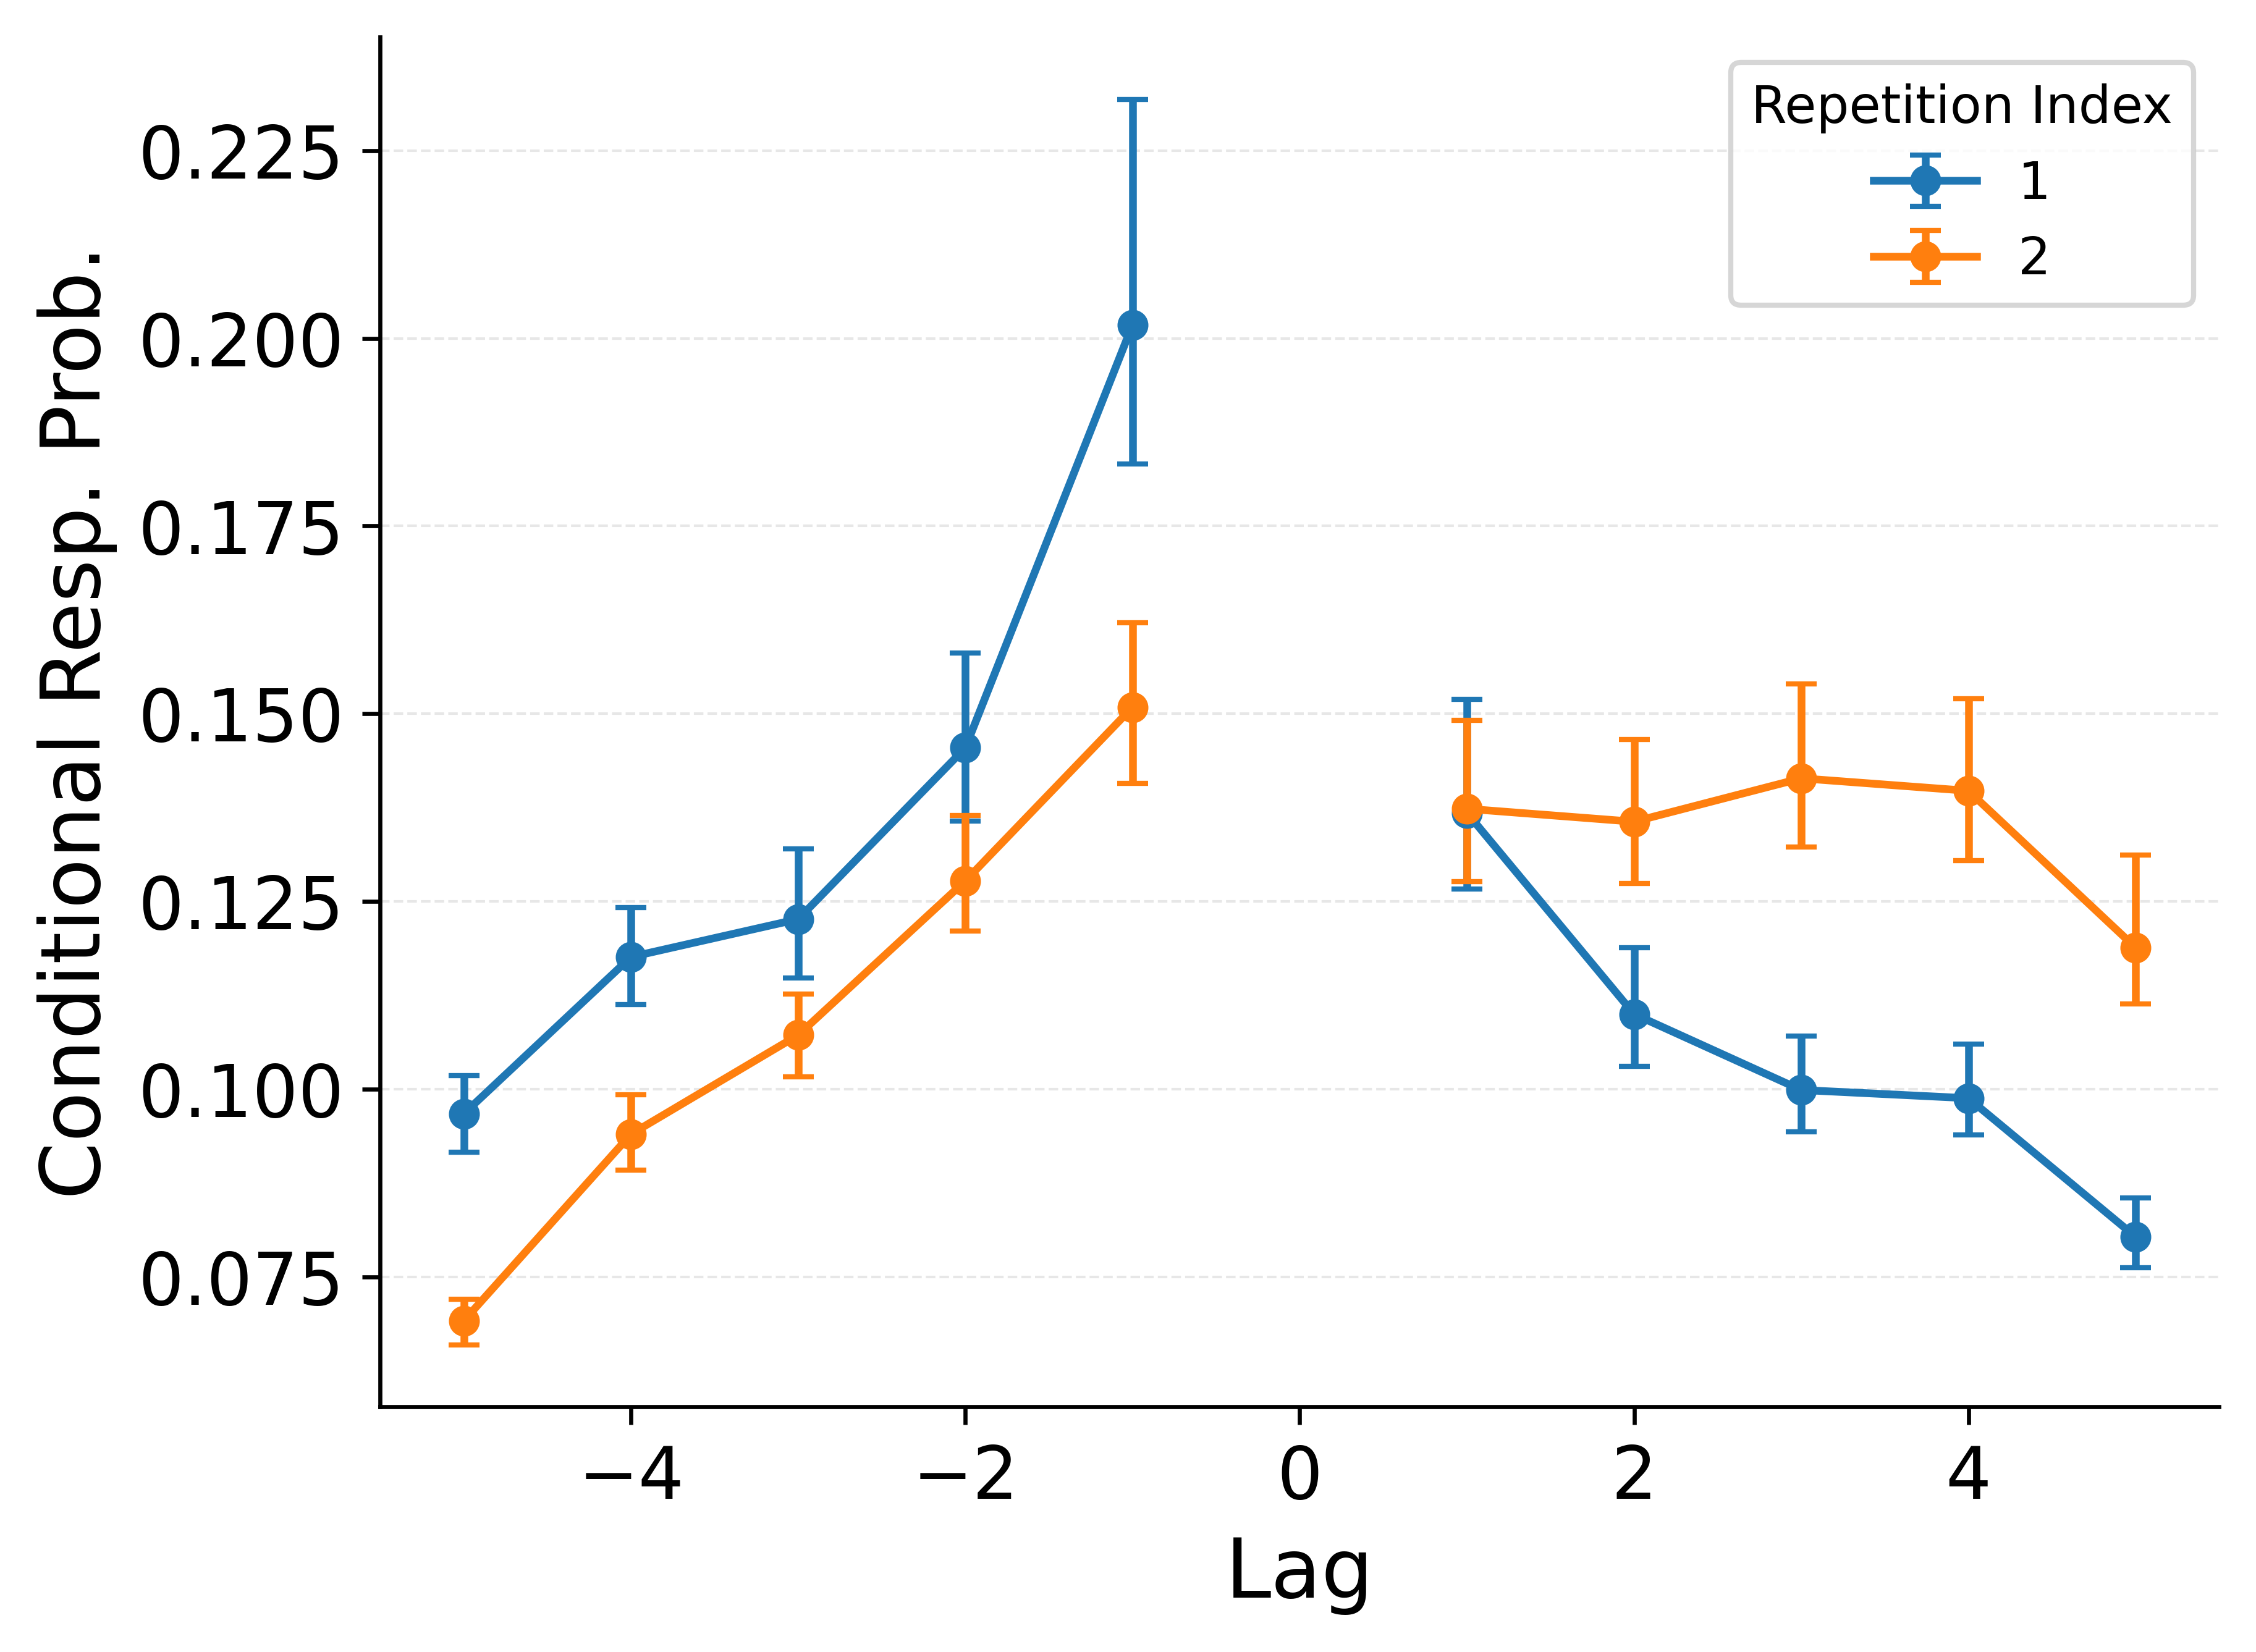
\includegraphics{../../work/thesis/figures/LohnasKahana2014_control_WeirdReinfPositionalCMR_full_best_of_3_LT34_back_rep_crp.png}\end{minipage}%

\end{figure}%

Finally, in serial recall, the same combination---distinct contexts at
study plus occurrence-specific reinstatement at test, with reinforcement
of the first occurrence---maintains strong continuations to \(i{+}1\)
and keeps cross-occurrence forward errors at baseline levels. The 2×2
comparison in Figure~\ref{fig-reinf_serial_rep_crp} uses Logan
(\citeproc{ref-logan2021serial}{2021}) (top: data; bottom: simulations)
and shows that ICMR-Reinf mirrors the empirically negligible elevation
of \(i\!\rightarrow\!j{+}1/j{+}2\) errors while preserving correct
forward chaining.

\begin{figure}

\caption{\label{fig-reinf_serial_rep_crp}Cross-occurrence forward errors
in serial recall (data vs ICMR-Reinf; Logan
(\citeproc{ref-logan2021serial}{2021}); Kahana and Jacobs
(\citeproc{ref-kahana2000interresponse}{2000})). Top: data; bottom:
ICMR-Reinf simulations. Panels plot, for items studied at \(i\) and
\(j\), the conditional probability---after correct report through
\(i\)---of erroneous transitions to the second occurrence's forward
neighbors (\(i\!\rightarrow\!j{+}1\) and \(i\!\rightarrow\!j{+}2\)),
contrasted with matched pseudo-repeater baselines. ICMR-Reinf reproduces
the data's non-elevation.}

\begin{minipage}{0.50\linewidth}
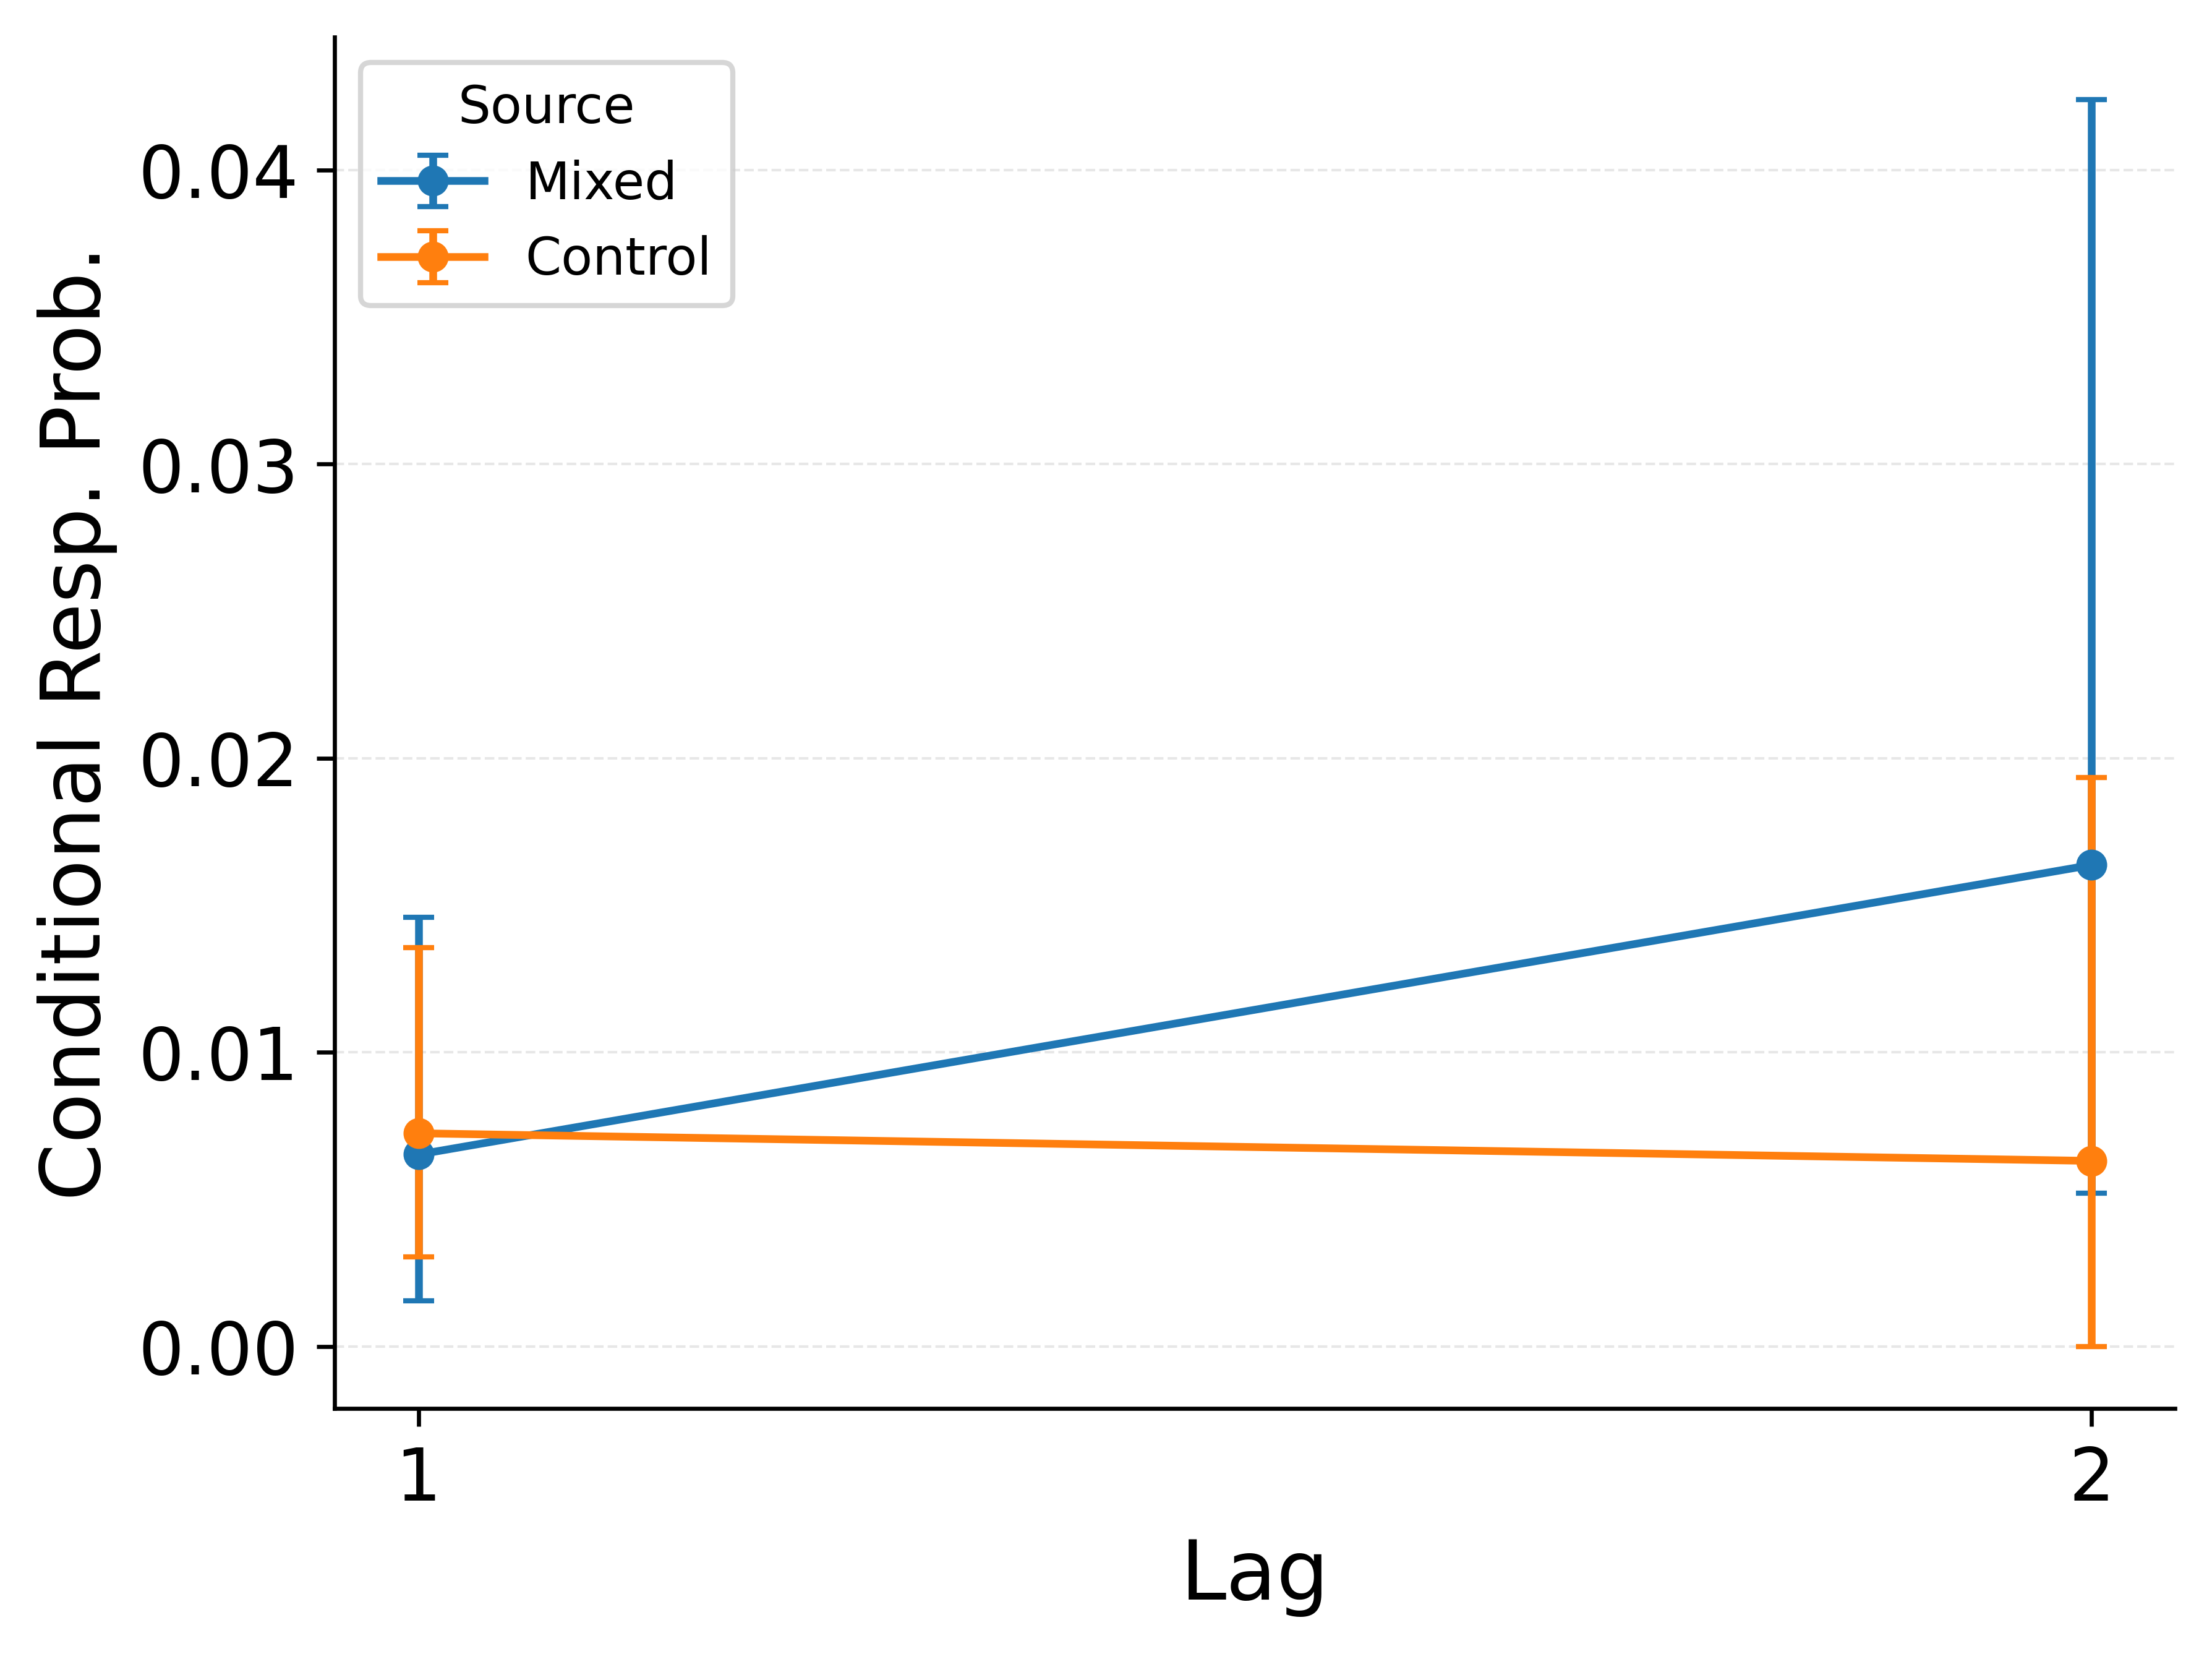
\includegraphics{../../work/thesis/figures/RepeatedRecallsGordonRanschburg2021_mixedvscontrolA_data_full_best_of_3_second_rep_crp.png}\end{minipage}%
%
\begin{minipage}{0.50\linewidth}
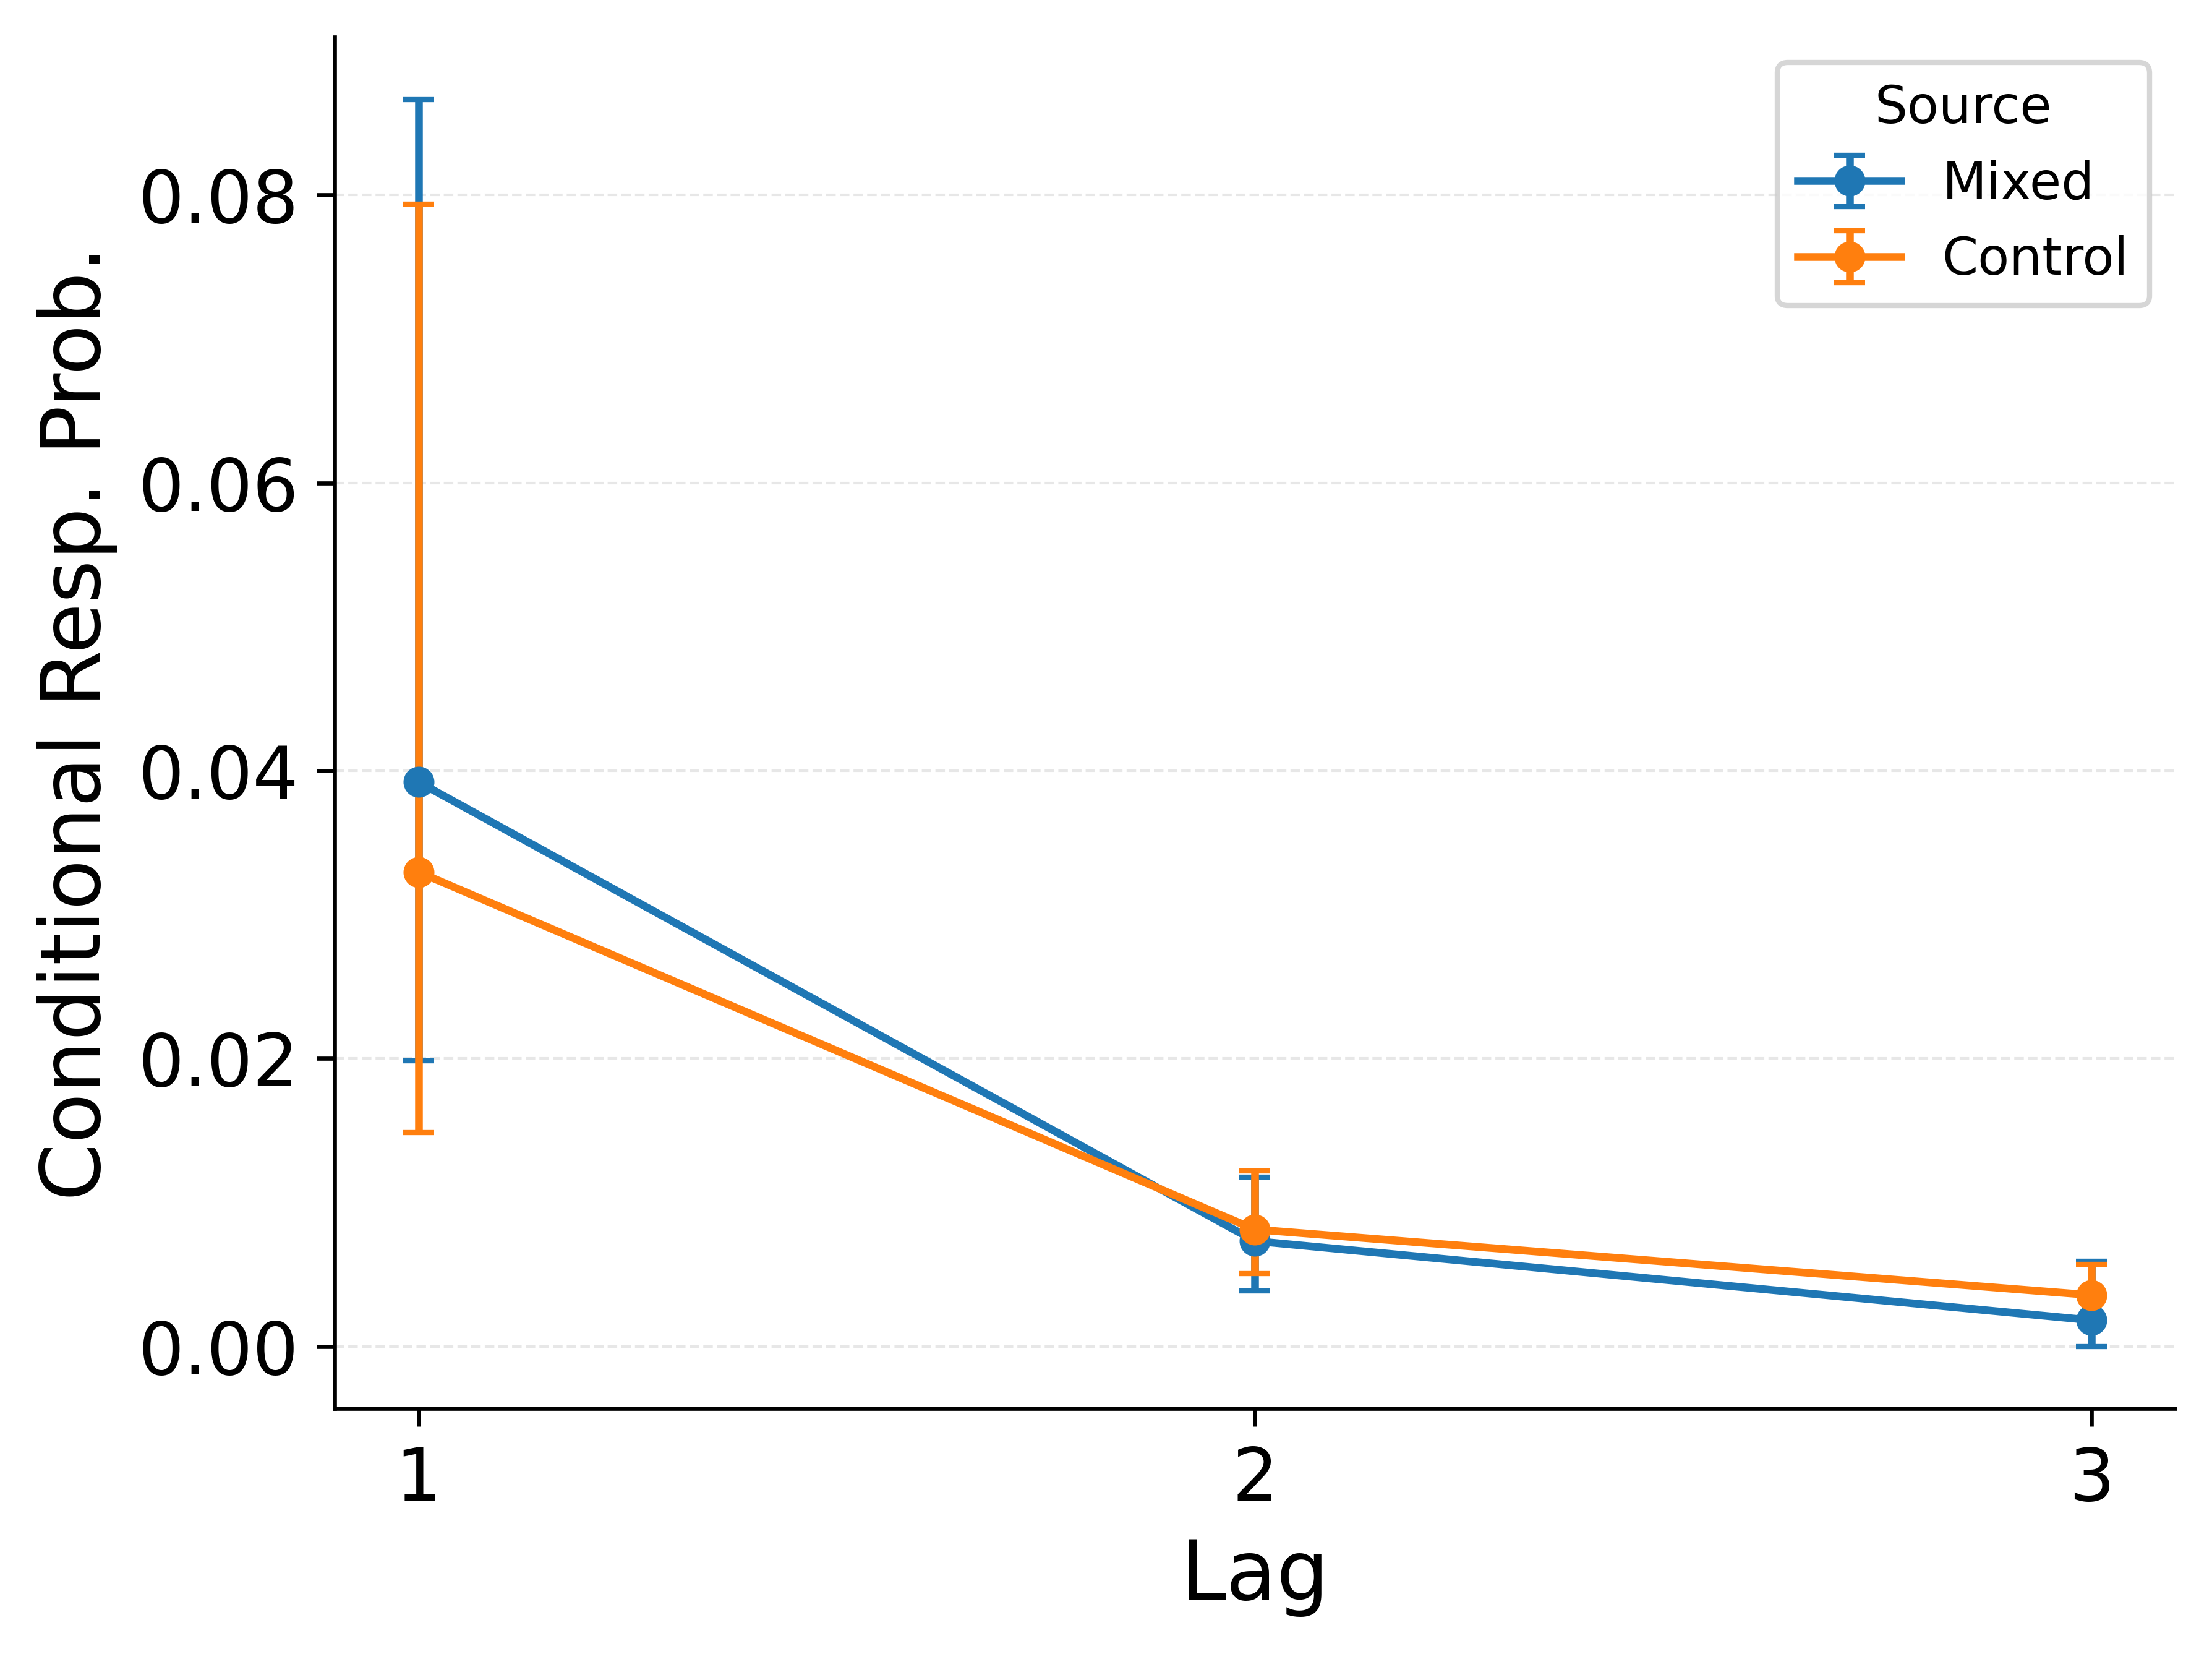
\includegraphics{../../work/thesis/figures/RepeatedRecallsKahanaJacobs2000_mixedvscontrolA_data_full_best_of_3_second_rep_crp.png}\end{minipage}%
\newline
\begin{minipage}{0.50\linewidth}
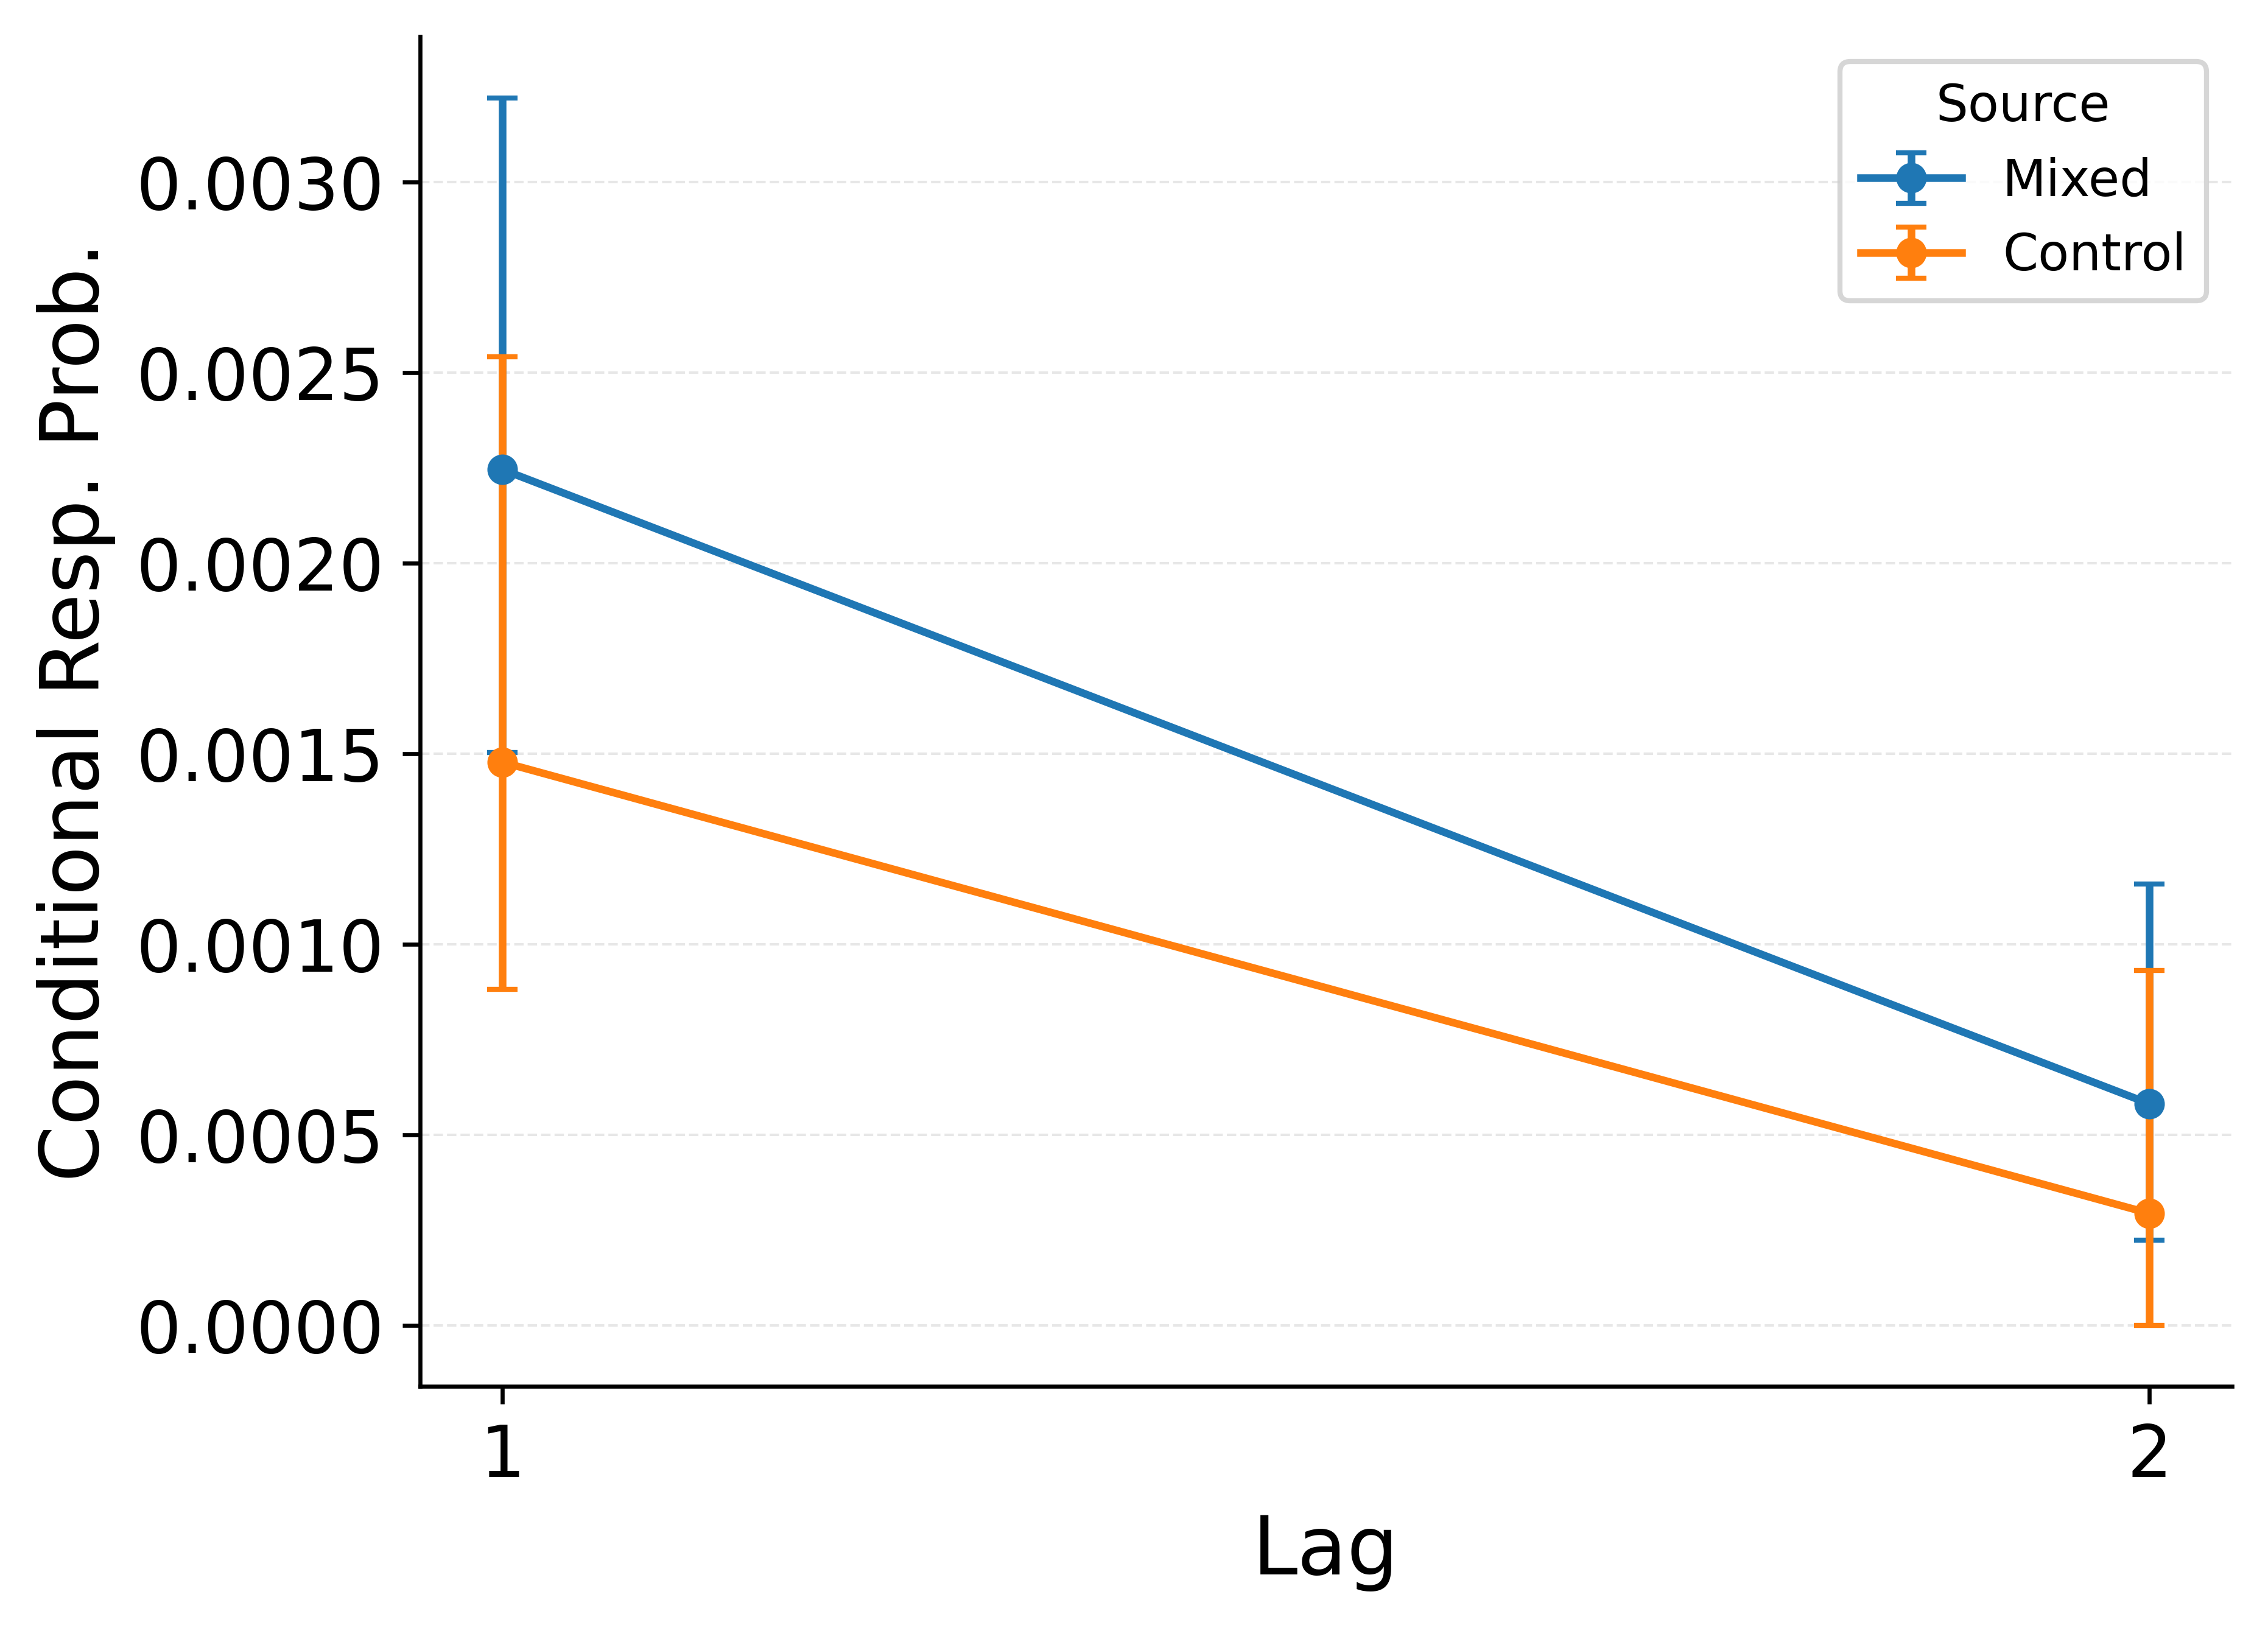
\includegraphics{../../work/thesis/figures/RepeatedRecallsGordonRanschburg2021_mixedvscontrolA_WeirdReinfPositionalCMR_full_best_of_3_second_rep_crp.png}\end{minipage}%
%
\begin{minipage}{0.50\linewidth}
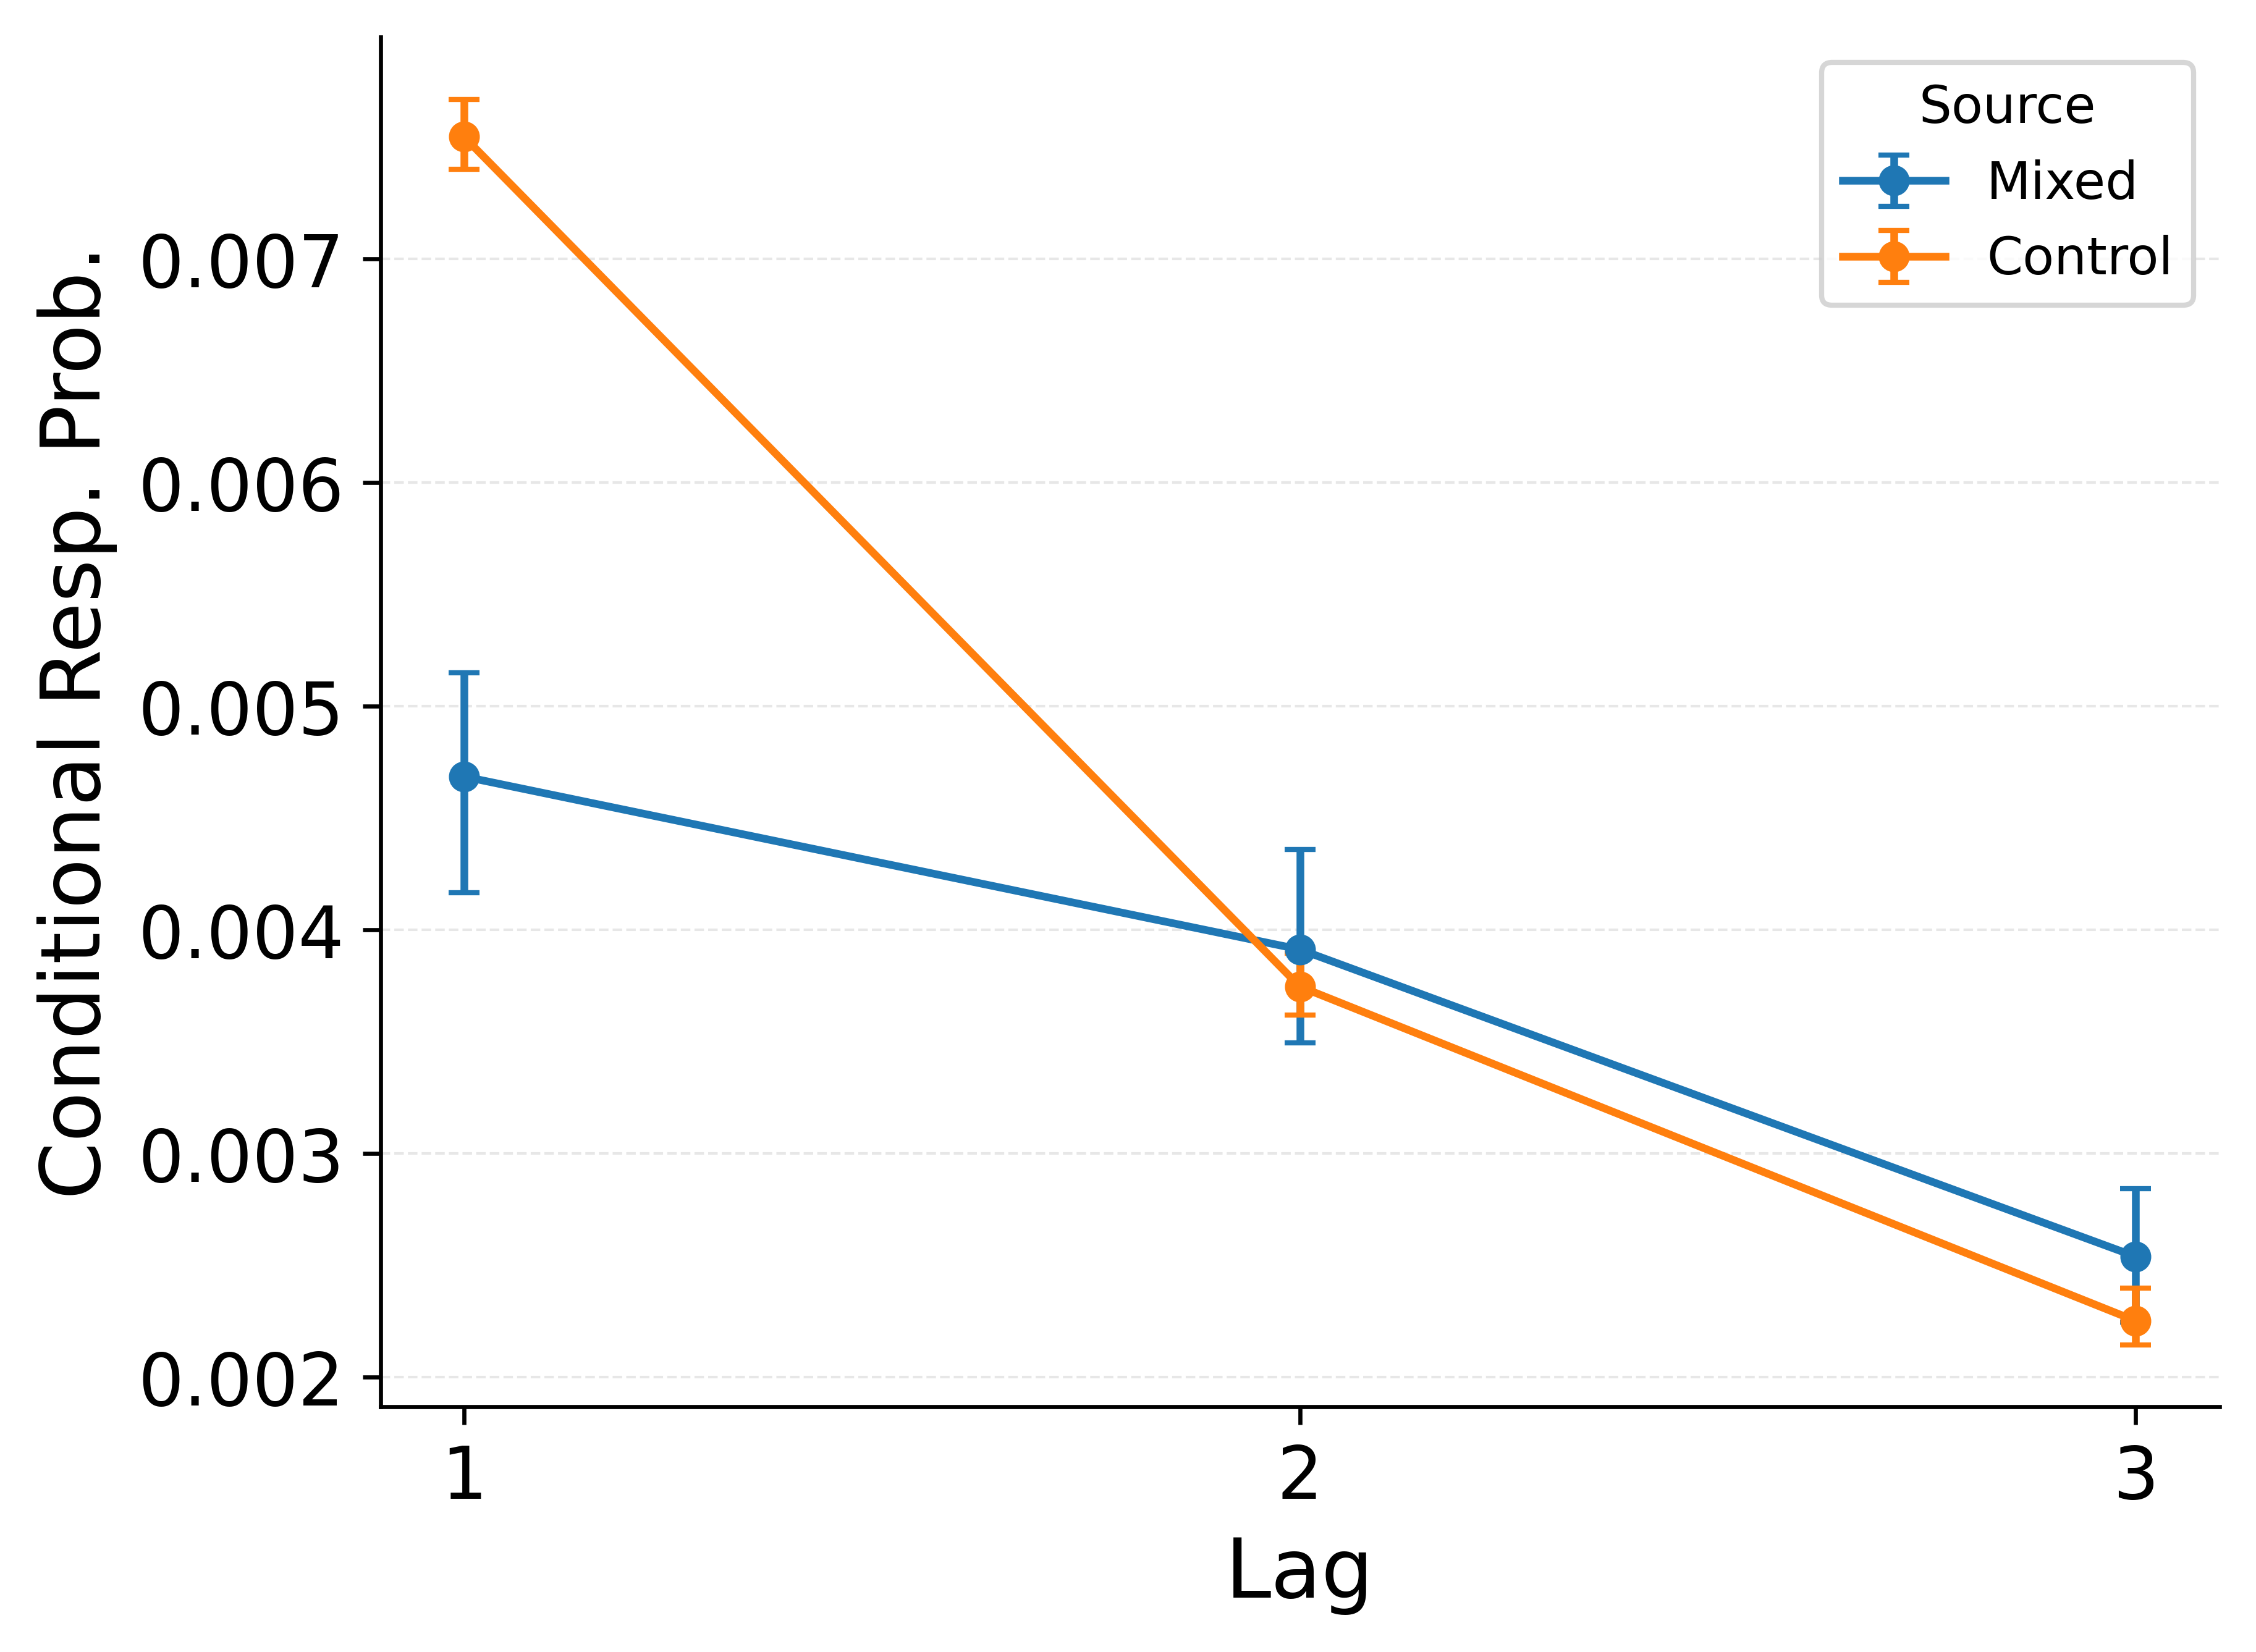
\includegraphics{../../work/thesis/figures/RepeatedRecallsKahanaJacobs2000_mixedvscontrolA_WeirdReinfPositionalCMR_full_best_of_3_second_rep_crp.png}\end{minipage}%

\end{figure}%

ICMR-Reinf keeps occurrences separate at study and allows retrieval to
select a single occurrence at test, while preferentially reinforcing the
first occurrence's trace. It preserves core benchmarks and the spacing
function; it maintains the absence of cross-neighbor knitting; it
resolves the outgoing lag-CRP blending and captures the boosted
first-over-second separation in mixed lists; and it mirrors the
non-interference pattern in serial recall. The price is a single
reinforcement parameter. The payoff is a coherent account in which a
rehabilitated, non-associative study-phase mechanism contributes to
repetition effects without reintroducing associative interference.

\subsection{Formal Comparison Across
Datasets}\label{formal-comparison-across-datasets}

We compared four variants under a common fitting and scoring pipeline
(Methods): Standard CMR , ICMR-NoSPR , Instance-CMR, and ICMR-Reinf.
ICMR-Reinf introduces one additional reinforcement parameter; all other
pairwise comparisons are parameter-matched. Fit quality is reported as
mean negative log-likelihood (−log\,L) across participants with
bootstrapped 95\% CIs over subjects. Where informative, we also report
AIC model weights (AICw), which penalize parameter count.

Across datasets, three patterns emerge. First, Instance-CMR
substantially improves fit relative to Standard CMR in all datasets,
with especially large gains in the serial-recall tasks
(\citeproc{ref-kahana2000interresponse}{Kahana \& Jacobs, 2000};
\citeproc{ref-logan2021serial}{Logan, 2021}). Second, adding study-phase
reinforcement without contextual knitting (ICMR-Reinf) yields a further,
reliable improvement in free recall (Lohnas and Kahana
(\citeproc{ref-lohnas2014retrieved}{2014}); Broitman and Kahana
(\citeproc{ref-broitman2024neural}{2024})) despite its extra parameter,
but brings no advantage over OS in serial recall. Third, ICMR-NoSPR
improves over Standard CMR in free recall but is not sufficient on its
own---consistent with the results sections above.

\begin{table}

{\caption{{\textbf{Free‑recall model fits (−log\,L; lower is better).}
Values are participant means ± bootstrapped 95\% CIs
(subjects).}{\label{tbl-fit-fr}}}
\vspace{-20pt}}

\begin{longtable}[]{@{}lrr@{}}
\toprule\noalign{}
Model variant & Lohnas and Kahana
(\citeproc{ref-lohnas2014retrieved}{2014}) & Broitman and Kahana
(\citeproc{ref-broitman2024neural}{2024}) \\
\midrule\noalign{}
\endhead
\bottomrule\noalign{}
\endlastfoot
Standard CMR & 1668.19 ± 146.93 & 1268.71 ± 279.66 \\
ICMR‑NoSPR & 1661.98 ± 146.77 & 1263.46 ± 277.99 \\
ICMR‑OS & 1661.01 ± 147.02 & 1260.15 ± 278.41 \\
ICMR‑Reinf & \textbf{1658.99 ± 146.97} & \textbf{1259.17 ± 278.37} \\
\end{longtable}

\end{table}

\begin{table}

{\caption{{\textbf{Serial‑recall model fits (−log\,L; lower is better).}
ICMR‑NoSPR was not evaluated for the serial‑recall datasets. Values are
participant means ± bootstrapped 95\% CIs
(subjects).}{\label{tbl-fit-sr}}}
\vspace{-20pt}}

\begin{longtable}[]{@{}lrr@{}}
\toprule\noalign{}
Model variant & Logan (\citeproc{ref-logan2021serial}{2021}) & Kahana
and Jacobs (\citeproc{ref-kahana2000interresponse}{2000}) \\
\midrule\noalign{}
\endhead
\bottomrule\noalign{}
\endlastfoot
Standard CMR & 770.66 ± 59.75 & 3852.12 ± 530.13 \\
ICMR‑OS & \textbf{729.19 ± 60.18} & \textbf{3759.75 ± 516.93} \\
ICMR‑Reinf & 730.08 ± 60.47 & 3761.08 ± 516.74 \\
\end{longtable}

\end{table}

As compact deltas relative to Standard CMR: Lohnas −log\,L improves by
\textbf{−6.21} (NoSPR), \textbf{−7.18} (OS), \textbf{−9.20} (Reinf);
Broitman by \textbf{−5.25}, \textbf{−8.56}, \textbf{−9.54}; Logan
(serial) by \textbf{−41.47} (OS) and \textbf{−40.58} (Reinf); Kahana \&
Jacobs (serial) by \textbf{−92.37} (OS) and \textbf{−91.04} (Reinf).

To separate parameter-count effects from fit, we report AICw in two
steps. First, a \textbf{pairwise} comparison between
\textbf{Instance-CMR} and \textbf{Standard CMR} (parameter-matched)
across all datasets; second, a \textbf{three-way} comparison in free
recall that \textbf{includes ICMR-Reinf} (adds one parameter).

\begin{table}

{\caption{{\textbf{Pairwise AIC weights (Instance-CMR vs Standard CMR).}
OS is preferred in every dataset.}{\label{tbl-aic-os-vs-cmr}}}
\vspace{-20pt}}

\begin{longtable}[]{@{}lrr@{}}
\toprule\noalign{}
Dataset & AICw (Standard) & AICw (Instance-CMR) \\
\midrule\noalign{}
\endhead
\bottomrule\noalign{}
\endlastfoot
Lohnas and Kahana (\citeproc{ref-lohnas2014retrieved}{2014}) &
3.25\,×\,10⁻¹¹⁰ & \textbf{1.00} \\
Broitman and Kahana (\citeproc{ref-broitman2024neural}{2024}) &
8.24\,×\,10⁻¹²⁴ & \textbf{1.00} \\
Logan (\citeproc{ref-logan2021serial}{2021}) & 0 & \textbf{1.00} \\
Kahana and Jacobs (\citeproc{ref-kahana2000interresponse}{2000}) & 0 &
\textbf{1.00} \\
\end{longtable}

\end{table}

\begin{table}

{\caption{{\textbf{Three-way AIC weights in free recall.} After
penalization, ICMR-Reinf is preferred; OS is second; Standard CMR is not
competitive.}{\label{tbl-aic-fr}}}
\vspace{-20pt}}

\begin{longtable}[]{@{}
  >{\raggedright\arraybackslash}p{(\columnwidth - 6\tabcolsep) * \real{0.5000}}
  >{\raggedleft\arraybackslash}p{(\columnwidth - 6\tabcolsep) * \real{0.1667}}
  >{\raggedleft\arraybackslash}p{(\columnwidth - 6\tabcolsep) * \real{0.1667}}
  >{\raggedleft\arraybackslash}p{(\columnwidth - 6\tabcolsep) * \real{0.1667}}@{}}
\toprule\noalign{}
\begin{minipage}[b]{\linewidth}\raggedright
Free-recall dataset
\end{minipage} & \begin{minipage}[b]{\linewidth}\raggedleft
AICw (Standard)
\end{minipage} & \begin{minipage}[b]{\linewidth}\raggedleft
AICw (Instance-CMR)
\end{minipage} & \begin{minipage}[b]{\linewidth}\raggedleft
AICw (ICMR-Reinf)
\end{minipage} \\
\midrule\noalign{}
\endhead
\bottomrule\noalign{}
\endlastfoot
Lohnas and Kahana (\citeproc{ref-lohnas2014retrieved}{2014}) &
1.91\,×\,10⁻¹⁴⁰ & 5.87\,×\,10⁻³¹ & \textbf{1.00} \\
Broitman and Kahana (\citeproc{ref-broitman2024neural}{2024}) &
1.95\,×\,10⁻¹³⁷ & 2.37\,×\,10⁻¹⁴ & \textbf{1.00} \\
\end{longtable}

\end{table}

As a complementary, model-agnostic summary, we report the fraction of
participants whose individual fit favored one model over another (lower
−log\,L). These ``win rates'' mirror the AIC results:
\textbf{Instance-CMR} beats Standard CMR for most or all participants in
every dataset (Lohnas \textbf{80\%}, Broitman \textbf{79\%}, Logan
\textbf{100\%}, Kahana \& Jacobs \textbf{100\%}). In \textbf{free
recall}, \textbf{ICMR-Reinf} beats Instance-CMR for a majority of
participants (Lohnas \textbf{63\%}, Broitman \textbf{64\%}), whereas in
\textbf{serial recall} the two are roughly tied (Logan \textbf{46\%} for
Reinf; Kahana \& Jacobs \textbf{53\%} for OS).

Taken together with the diagnostic analyses, the model-comparison
results support a simple division of labor. Occurrence-specific
reinstatement at test (Instance-CMR) is necessary to eliminate the
cross-occurrence interference predicted by Standard CMR and dominates in
serial recall. Study-phase reinforcement without contextual knitting
(ICMR-Reinf) adds a small but reliable advantage in free recall by
capturing the boosted access to first-occurrence context, while
preserving the non-interference profile. ICMR-NoSPR establishes that
CMR's original study-phase reinstatement is not required for overall
spacing or benchmark fits, but by itself it does not resolve the
interference signature. Across datasets, standard CMR is consistently
least favored under penalized fit.

\section{General Discussion}\label{general-discussion}

Human episodic search is strikingly organized by temporal contiguity:
recalling one experience tends to cue retrieval of experiences that
occurred nearby in time (\citeproc{ref-healey2019contiguity}{Healey et
al., 2019}; \citeproc{ref-kahana1996associative}{Kahana, 1996}). This
work asked how that organizing principle manifests when the same item
has multiple study positions within a list (e.g., ``canoe'' at positions
\emph{i} and \emph{j}). Do repetitions knit their occurrence‑specific
neighborhoods together, or do they remain separable such that retrieval
can route through one occurrence without contacting the other? We
addressed this question in free and serial recall by comparing
performance in lists with item repetitions to a position‑matched,
symmetric baseline. This procedure removes list-composition artifacts
and isolates the consequences of being a repetition rather than a novel
token in those positions (\citeproc{ref-lohnas2014retrieved}{Lohnas \&
Kahana, 2014}; \citeproc{ref-ratcliff1990list}{Ratcliff et al., 1990};
\citeproc{ref-tulving1972inhibition}{Tulving \& Hastie, 1972}).

Retrieved‑context models explain contiguity and related regularities by
coupling items to a slowly drifting temporal context and using that
context as both a storage address and a retrieval cue
(\citeproc{ref-healey2019contiguity}{Healey et al., 2019};
\citeproc{ref-howard2002distributed}{Howard \& Kahana, 2002a};
\citeproc{ref-polyn2009context}{Polyn et al., 2009}). During study,
presenting an item reinstates contextual features associated with it
into the ongoing context state, and the item binds to that updated
state. Because the context drifts, different occurrences of the same
item couple to different temporal states. During retrieval, the current
context preferentially cues items encoded in similar contexts. Recalling
an item then reinstates its associated contextual features into the cue
again, which pulls subsequent transitions toward items studied nearby in
time.

Under this framework, context evolution is item-driven. Presenting or
recalling an item retrieves its associated context features and pulls
the ongoing temporal context toward those item-specific features. This
commitment explains how memory search can be guided by successive
retrieval events, and also provides a cohesive account of how item
repetition impacts memory retrieval dynamics
(\citeproc{ref-howard2002distributed}{Howard \& Kahana, 2002a};
\citeproc{ref-lohnas2014retrieved}{Lohnas \& Kahana, 2014}). First, each
occurrence of the same item binds its to different temporal contexts;
with increased spacing, these contexts become more distinct, producing a
spacing advantage through encoding variability
(\citeproc{ref-cepeda2006distributed}{Cepeda et al., 2006};
\citeproc{ref-glenberg1979component}{Glenberg, 1979}). Second, each
occurrence triggers a form of study-phase retrieval: it partially
reinstates prior occurrences' contexts into the ongoing state, making
the contexts across occurrences more similar to each other
(\citeproc{ref-delaney2010spacing}{Delaney et al., 2010}; @
\citeproc{ref-hintzman1975spacing}{Hintzman et al., 1975}). Finally, at
test, recalling a repeated item reinstates a composite over its
occurrence-specific contexts, priming recall transitions toward
neighbors of all occurrences (\citeproc{ref-logan2021serial}{Logan,
2021}; \citeproc{ref-polyn2009context}{Polyn et al., 2009};
\citeproc{ref-sederberg2008context}{Sederberg et al., 2008}).

Here, we showed that this framework predicts patterns of
cross-occurrence associative interference in free and serial recall.
Item-driven context reinstatement knits occurrence-specific
neighborhoods together at encoding and test, producing three signatures
of blended support across occurrences. Together these imply that cues to
one occurrence should also cue the other, predicting that (i) recalling
a neighbor of one occurrence should cue neighbors of the other
occurrence (cross-occurrence neighbor transitions), (ii) recalling the
repeated item itself should produce balanced access to both occurrences'
neighborhoods, and (iii) in serial recall, correct chaining through one
occurrence should increase erroneous continuations to the other
occurrence's forward neighbors. But across multiple datasets, our
results contradict those predictions once the matched, symmetric
baseline is applied.

First, we found that cross-occurrence neighbor transitions sit at
baseline, indicating no knitting. Prior work
(\citeproc{ref-lohnas2014retrieved}{Lohnas \& Kahana, 2014}) reported
boosted cross-occurrence neighbor transitions in free recall, finding
that for repeated items with study positions \(i\) and \(j\),
participants exhibited boosted chances of transitioning from neighbors
of \(i\) (e.g., \(i{+}1,i{+}2\)) to neighbors of \(j\) (e.g.,
\(j{+}1,j{+}2\)) and vice versa compared to a control. We generalized
this analysis by reformulating it as a lag-CRP centered on the other
occurrence's neighbors and applying a matched, symmetric baseline to
control for list-composition effects. Despite a similar reported
methodology, our results observed no boost once the baseline was
applied, suggesting a potential confound in the original analysis.
Instead, what repetition effects we did observe were not predicted by
retrieved-context theory: a boosted chance of transitioning from
neighbors of the first occurrence to the repeated item itself
(lag\,=\,0) when it had not yet been recalled. Using a version of CMR
that integrates unique features into ongoing context whether study
events are new or repeated presentations keeps cross-occurrence neighbor
transitions at baseline but does not reproduce the lag\,=\,0 boost. A
further variant that preferentially strengthens the first occurrence's
trace upon item repetition captures this effect, suggesting a
non-associative mechanism that enhances access to the first occurrence
without knitting contexts together. These results challenge an
associative study-phase retrieval account of repetition's consequences
for memory search at study.

Second, we found that recalling the repeated item itself produced a
reliable preference for the first occurrence's neighbors over the
second's, contradicting the balanced-access prediction. Furthermore,
when considering incoming transitions to repeated items, arrivals from
the first occurrence's backward neighbor were more likely than from the
second's, again contradicting balanced access. These patterns have been
initially explored in other contemporaneous work. Broitman and Kahana
(\citeproc{ref-broitman2024neural}{2024}) focused on transitions from
repeated items in free recall, finding that they exhibit similar biases
toward the first occurrence's context and even observing in spectral EEG
analyses that neural activity patterns prior to these recall events were
most similar to patterns observed during the first occurrence's study
event. Similarly, Lohnas (\citeproc{ref-lohnas2025temporal}{2025})
examined incoming transitions to repeated items, finding that arrivals
from the first occurrence's backward neighbor were more likely than from
the second's.

Our results replicate and extend these findings, showing that they
persist across multiple datasets and are not artifacts of list
composition and clarifying them against a position-matched, symmetric
baseline. We found that these patterns are not fully accounted for by
standard CMR when considered in combination with outcomes of analyses on
a position-matched, symmetric baseline. Whereas CMR predicts more
balanced transitions from the repeated item to each occurrence's
neighbors compared to position-matched controls, our results show a
reliable preference for the first occurrence's neighbors that exceeds
baseline expectation. Using a version of CMR that both keeps occurrence
contexts separate at study and allows retrieval to select a single
occurrence's context at test is able eliminate CMR's prediction of
balanced access. However, the variant still does not capture the boosted
first-over-second separation in mixed lists relative to baseline. Our
variant that preferentially strengthens the first occurrence's trace
upon item repetition is able to additionally capture this preference,
suggesting that a non-associative mechanism enhances access to the first
occurrence without knitting contexts together. These results echo the
interpretation of similar patterns observed by Lohnas
(\citeproc{ref-lohnas2025temporal}{2025}), who argued that the first
occurrence may be privileged because retrieval of item information from
its first presentation upon its second presentation may strengthens its
trace. However, by contrast to Lohnas
(\citeproc{ref-lohnas2025temporal}{2025}), we find that
retrieved-context theory requires modification in order to instantiate
this mechanism without reintroducing associative interference.

Finally, we considered transitions from recall of repeated items in the
context of serial recall. In serial recall of sequences with item
repetitions, if recall proceeds accurately up through a repeated item's
first presentation, we asked how often participants erroneously
transition to the +1 neighbor of the item's \emph{second} presentation.
Because CMR predicts that recalling the repeated item reinstates a
composite over both occurrences' contexts, it predicts that correct
chaining through the first occurrence should increase erroneous
continuations to the second occurrence's forward neighbors. In contrast,
we found that such cross-occurrence forward errors were not elevated
above a position-matched, symmetric baseline in two independent
serial-recall datasets. This type of error receives extensive attention
in the serial-recall literature and has been central to critiques of
chaining models of serial order memory positing that each item cues the
next (\citeproc{ref-henson1996unchained}{Henson, 1996};
\citeproc{ref-kahana2000interresponse}{Kahana \& Jacobs, 2000}). These
results extend the same critique to retrieved-context models using an
item-based context reinstatement rule. Because they knit
occurrence-specific contexts together at study and test, they predict
that correct chaining through one occurrence should increase erroneous
continuations to the other occurrence's forward neighbors.

These findings provide a measured challenge to the standard
retrieved-context account of memory search. Retrieved-context theory
posits that context evolves by retrieving prior contextual states as
opposed to contemporaneous accounts that instead proposed that context
drifts randomly (\citeproc{ref-howard2002distributed}{Howard \& Kahana,
2002a}). Here, items are the drivers of context evolution, evoking
features from their prior presentations to update the ongoing context
state and guide retrieval. This framework was embraced as a more
parsimonious way to account for recency and contiguity effects in memory
using a single mechanism. But these data show that this mechanism,
however parsimonious, predicts associative interference that is not
observed empirically. They raise the question: what then becomes of
retrieved-context theory?

Our modeling results identify narrow changes to a retrieved-context
model that reconcile it with these findings. Removing associative
study-phase retrieval (CMR‑NoSPR) abolishes cross‑occurrence neighbor
linkage yet preserves serial‑position, CRP, and spacing benchmarks,
showing that classic free‑recall successes do not depend on item-driven
context evolution as originally implemented. Allowing
occurrence‑specific reinstatement at test (ICMR‑OS) then eliminates
balanced access from the repeater and preserves forward chaining in
serial recall. It sidesteps the associative‑interference prediction
while keeping the temporal‑context machinery intact. These changes are
effectively a variant of CMR that replaces item-based context and
retrieval dynamics with an occurrence-specific alternative that can be
variously interpreted as using a position-, event-, instance- or
timeline-based code. Here, item identities are only relevant when
reporting the recalled item; they do not associate study events during
encoding or memory search. The resulting variant is still a
retrieved-context model because it still posits that context evolves by
retrieving prior contextual states, but treats each study episode as a
unique event that can be separately cued and retrieved at test.

The serial‑recall literature has long emphasized positional or timeline
codes and competitive selection to explain transposition gradients and
the sparing of strict chaining, particularly in lists with within‑list
repetitions (\citeproc{ref-brown2000oscillator}{Brown et al., 2000};
\citeproc{ref-henson1996unchained}{Henson, 1996}). Our serial‑recall
analyses align with this perspective: after correct report through the
first occurrence, continuations to \emph{i\,+\,1} were preserved and
erroneous continuations to the competing neighbor \emph{j\,+\,1} were
not elevated relative to position‑matched controls -- exactly the
pattern positional accounts anticipate and that strict item‑to‑item
chaining (or blended item‑based reinstatement) would struggle to
accommodate. In other words, the absence of cross‑occurrence forward
errors in our data is not merely compatible with positional coding; it
is diagnostic of the kind of competition over position‑like cues those
models posit. Traditionally, accounts of free recall have de-emphasized
the role of positional information, with performance thought to rely
predominantly on temporal coding and semantic organization
(\citeproc{ref-lohnas2015expanding}{Lohnas et al., 2015};
\citeproc{ref-polyn2009context}{Polyn et al., 2009};
\citeproc{ref-sederberg2008context}{Sederberg et al., 2008}). However,
recent efforts to show that retrieved-context models can address serial
as well as free recall (\citeproc{ref-logan2021serial}{Logan, 2021};
\citeproc{ref-lohnas2024retrieved}{Lohnas, 2024}) have highlighted the
viability of an integrated framework that encompasses both types of
recall. These results help advance an integrated view of serial and free
recall where a common set of constraints from both literatures inform
theory development. The resulting model retains the core principles of
retrieved-context theory while incorporating insights from positional
coding approaches: it allows for the use of position-like information to
guide retrieval while maintaining the evolving context representation as
the primary search scaffold.

It is nonetheless challenging to reconcile these findings with prior
demonstrations that item features can influence organization in free and
serial recall. Free recall is classically subject to semantic
organization, a tendency for similar items to cluster during retrieval
(\citeproc{ref-bousfield1953occurrence}{Bousfield, 1953};
\citeproc{ref-glanzer1969distance}{Glanzer, 1969};
\citeproc{ref-howard2002does}{Howard \& Kahana, 2002b};
\citeproc{ref-romney1993predicting}{Romney et al., 1993}). Similarly,
serial-recall performance is influenced by item-level properties such as
phonological similarity (\citeproc{ref-baddeley1966influence}{Baddeley,
1966}; \citeproc{ref-osth2023item}{Osth \& Hurlstone, 2023}). This
consistency of these classic benchmarks establishes all but
incontrovertibly that item features fundamentally influence the
organization of memory search, instead of just defining what is reported
when a trace is retrieved. Furthermore, patterns of prior-list
intrusions (PLIs) across free and serial recall suggest that items can
cue retrieval across list boundaries, which is difficult to reconcile
with a purely temporal or positional code. For example, transitions from
items in the prior list to their neighbors in the current list are
elevated relative to a matched baseline, suggesting that item features
can cue retrieval across list boundaries
(\citeproc{ref-lohnas2015expanding}{Lohnas et al., 2015}). At the same
time though, positional codes have been shown to influence PLIs in
serial recall, with intrusions tending to come from the same serial
position in the prior list as the current recall position (e.g.,
\citeproc{ref-osth2023item}{Osth \& Hurlstone, 2023}). Together, a
wealth of evidence persistently shows that item features influence
organization in both free and serial recall.

Logan (\citeproc{ref-logan2021serial}{2021}) demonstrated item-dependent
and position-dependent contexts can be accommodated simultaneously in a
retrieved-context model to simultaneously address these and other
constraints. Similarly, CMR and its variants has traditionally included
multiple layers of context that encode different kinds of similarity
relationships across study events, such as a semantic layer that
captures item similarity or a source layer that captures stimulus
modality (\citeproc{ref-polyn2009context}{Polyn et al., 2009}). Given
these successes, it is likely that ICMR-OS could similarly be extended
to include item-level features alongside the occurrence-specific
features it applies to avoid associative interference. An additional
parameter that weights the contribution of an item-dependent contextual
layer relative to a occurrence-specific contextual layer could allow the
model to flexibly capture the influence of item features on organization
while avoiding associative interference across occurrences.

That said, the lack of any cross‑occurrence interference in our free‑
and serial‑recall datasets weighs against even a ``small'' but pervasive
role for item‑based knitting in the organization of search under
standard list‑learning conditions. These results instead tentatively
endorse a model that completely excludes item-level features from
driving context evolution during encoding or retrieval. Two caveats
temper these conclusions. First, we did not systematically analyze
individual differences in cross‑occurrence interference; if a minority
of participants show blending, population‑level averages could mask it.
Second, we did not report evaluation of mixture models that combine
explicit position/timeline codes with limited item‑based inputs under a
single architecture. Either extension could clarify when item‑based
features influence organization -- e.g., under deliberate integration
instructions, at very short lags with rehearsal, or when semantic
scaffolds promote cross‑episode binding. A program of research that
evaluates proposed models across a broader range of conditions and
datasets and addresses phenomena like PLIs and semantic clustering could
similarly clarify when item-level features influence organization. These
limitations set the stage for future work.

Along with its consequences for retrieved-context accounts of memory
search, these results also challenge classic understanding of factors
underlying the spacing effect. The spacing effect is classically
understood as a repetition effect, and has been a central focus of
research on memory for repeated experience
(\citeproc{ref-cepeda2006distributed}{Cepeda et al., 2006}) However, it
applies even to pairs of distinct items, not just repeated items. By
measuring the probability of retrieving either of two study items during
a free recall trial -- an analysis termed the ``OR score'' -- research
consistently finds that pairs of spaced items were more likely to be
recalled than pairs of massed items
(\citeproc{ref-lohnas2011contextual}{Lohnas et al., 2011}). Notably, in
a phenomenon called ``superadditivity'', the mnenomic benefit of spacing
tends to be more pronounced for repeated items than for distinct items .
The probability of recalling an item repeated in a spaced fashion is
frequently reported as higher than the probability of recalling one of
two distinct but similarly spaced items, violating statistical
independence (\citeproc{ref-benjamin2010distributed}{Benjamin \& Tullis,
2010}). This has been interpreted as evidence that additional mechanisms
are at play when items are repeated, beyond those that govern the
spacing effect for distinct items. Our results did not directly test for
a superadditive spacing effect, but nonetheless provide insight into its
possible mechanisms.

The study-phase retrieval hypothesis is one among several prominent
accounts of where such a superadditive spacing advantage might come
from. By this account, presenting an item again after a lag reinstates
the context associated with its prior presentation, in some way
strengthening access to the item's representation in memory
(\citeproc{ref-delaney2010spacing}{Delaney et al., 2010};
\citeproc{ref-hintzman1975spacing}{Hintzman et al., 1975}).
Retrieved-context theory combines a specific instantiation of this idea
with a contextual variability mechanism to explain the spacing effect
for repeated items (\citeproc{ref-howard2002distributed}{Howard \&
Kahana, 2002a}; \citeproc{ref-lohnas2014retrieved}{Lohnas \& Kahana,
2014}). In retrieved-context models, study-phase retrieval during
repetition reinstates makes the contexts across occurrence neighborhoods
more similar to each other, producing the patterns of associative
interference described above. This mechanism has been proposed to help
address spacing effects in free recall
(\citeproc{ref-lohnas2014retrieved}{Lohnas \& Kahana, 2014}) as well as
a potential basis for the benefits of retrieval practice
(\citeproc{ref-karpicke2011retrieval}{Karpicke \& Blunt, 2011};
\citeproc{ref-whiffen2017role}{Whiffen \& Karpicke, 2017b}). But while
confirming and evaluating CMR's predictions of associative interference
because of this mechanism, we also showed that study-phase retrieval in
CMR does not contribute to the spacing effect itself: removing the
mechanism (in CMR-SPR) preserves the spacing advantage for repeated
items and keeps contexts reinstated upon each occurrence distinct. In
CMR, the primary consequence of study-phase retrieval is to knit
occurrence-specific contexts together; characterizations of the
mechanism as providing a repetition-specific strengthening of retrieved
representations are not clearly supported by the current findings
(\citeproc{ref-lohnas2025temporal}{Lohnas, 2025};
\citeproc{ref-lohnas2014retrieved}{Lohnas \& Kahana, 2014}).

To match this characterization, we proposed a modified version of
ICMR-OS (ICMR-Reinf) that explicitly incorporates study-phase retrieval
as a mechanism for strengthening representations during repetition. When
an item is repeated, it preferentially strengthens the trace of the
first occurrence without knitting contexts together, using an additional
parameter to control the degree of strengthening. This mechanism
accounts for three patterns identified in our analyses. First, it
captures the boosted access to the first occurrence's neighbors upon
recalling the repeated item itself in free recall. Second, it captures
the boosted probability of transition to repeated items from the -1
neighbor of the first occurrence relative to the second. Third, it
captures the boosted tendency after retrieving the +1 neighbor of an
item's first occurrence to transition to the repeated item itself when
it has not yet been recalled. All these patterns can be accounted for in
terms of strengthened context-to-item associations for the first
occurrence of any repeatedly studied items without cross-occurrence
knitting. Still, model fits are not substantially improved over ICMR-OS
by this variant, suggesting that further development is needed to
interpret these patterns and their mechanistic basis. Instead,
ICMR-Reinf represents an example of how study-phase retrieval might be
rehabilitated within retrieved-context models to capture
repetition-specific effects without reintroducing associative
interference.

This work opened by asking how memory links related episodes without
collapsing their distinctive details. In an example scenario, we
described two visits to a bakery: one where you inhale warm cinnamon and
buy a fresh loaf, and another where you are greeted by the aroma of
espresso and a new cashier. How is it that a friend speaking of ``the
bakery down the street'' can remind you of both visits, yet you still
know which purchase happened when? The standard retrieved-context
account of memory search posits that this is a task fraught with
interference, because such a cue can retrieve a blend of contextual
details across both visits. In contrast, our results suggest that memory
search in tasks like free and serial recall succeeds by sidestepping
this challenge. Instead of using item features to remember associated
contextual details, memory search may rely on a positional or
event-based contextual code that can separately index each occurrence of
an item during encoding and later retrieve individual occurrences stored
as distinct traces at test. A later mention of ``the bakery down the
street'' can cue either visit, but it need not blend them. Memory search
can route through one episode at a time, preserving what happened when,
allowing repeated experience to strengthen access without sacrificing
specificity.

\section{References}\label{references}

\phantomsection\label{refs}
\begin{CSLReferences}{1}{0}
\bibitem[\citeproctext]{ref-anderson1995introduction}
Anderson, J. A. (1995). \emph{An introduction to neural networks}. MIT
press.

\bibitem[\citeproctext]{ref-baddeley1966influence}
Baddeley, A. D. (1966). The influence of acoustic and semantic
similarity on long-term memory for word sequences. \emph{The Quarterly
Journal of Experimental Psychology}, \emph{18}(4), 302--309.

\bibitem[\citeproctext]{ref-benjamin2010distributed}
Benjamin, A. S., \& Tullis, J. G. (2010). What makes distributed
practice effective? \emph{Cognitive Psychology}, \emph{61}(3), 228--247.
\url{https://doi.org/10.1016/j.cogpsych.2010.05.004}

\bibitem[\citeproctext]{ref-bousfield1953occurrence}
Bousfield, W. A. (1953). The occurrence of clustering in the recall of
randomly arranged associates. \emph{The Journal of General Psychology},
\emph{49}(2), 229--240.

\bibitem[\citeproctext]{ref-bower1972coding}
Bower, G., Melton, A., \& Martin, E. (1972). \emph{Coding processes in
human memory}.

\bibitem[\citeproctext]{ref-broitman2024neural}
Broitman, A. W., \& Kahana, M. J. (2024). Neural context reinstatement
of recurring events. \emph{bioRxiv}.

\bibitem[\citeproctext]{ref-brown2000oscillator}
Brown, G. D., Preece, T., \& Hulme, C. (2000). Oscillator-based memory
for serial order. \emph{Psychological Review}, \emph{107}(1), 127.

\bibitem[\citeproctext]{ref-cepeda2006distributed}
Cepeda, N. J., Pashler, H., Vul, E., Wixted, J. T., \& Rohrer, D.
(2006). Distributed practice in verbal recall tasks: A review and
quantitative synthesis. \emph{Psychological Bulletin}, \emph{132}(3),
354.

\bibitem[\citeproctext]{ref-cox2020similarity}
Cox, G. E., \& Criss, A. H. (2020). Similarity leads to correlated
processing: A dynamic model of encoding and recognition of episodic
associations. \emph{Psychological Review}, \emph{127}(5), 792.

\bibitem[\citeproctext]{ref-delaney2010spacing}
Delaney, P. F., Verkoeijen, P. P., \& Spirgel, A. (2010). Spacing and
testing effects: A deeply critical, lengthy, and at times discursive
review of the literature. \emph{Psychology of Learning and Motivation},
\emph{53}, 63--147.

\bibitem[\citeproctext]{ref-estes1955statistical}
Estes, W. K. (1955). Statistical theory of spontaneous recovery and
regression. \emph{Psychological Review}, \emph{62}(3), 145.

\bibitem[\citeproctext]{ref-friendly1982toronto}
Friendly, M., Franklin, P. E., Hoffman, D., \& Rubin, D. C. (1982). The
toronto word pool: Norms for imagery, concreteness, orthographic
variables, and grammatical usage for 1,080 words. \emph{Behavior
Research Methods \& Instrumentation}, \emph{14}(4), 375--399.

\bibitem[\citeproctext]{ref-glanzer1969distance}
Glanzer, M. (1969). Distance between related words in free recall: Trace
of the STS. \emph{Journal of Verbal Learning and Verbal Behavior},
\emph{8}(1), 105--111.

\bibitem[\citeproctext]{ref-glenberg1979component}
Glenberg, A. M. (1979). Component-levels theory of the effects of
spacing of repetitions on recall and recognition. \emph{Memory \&
Cognition}, \emph{7}(2), 95--112.

\bibitem[\citeproctext]{ref-gunn2025bridging}
Gunn, J. B., \& Polyn, S. M. (2025). Bridging CRU and CMR in free and
serial recall: A factorial comparison of retrieved-context models.
\emph{The American Journal of Psychology}, \emph{138}(2), 203--230.
\url{https://doi.org/10.5406/19398298.138.2.09}

\bibitem[\citeproctext]{ref-healey2014memory}
Healey, M. K., \& Kahana, M. J. (2014). Is memory search governed by
universal principles or idiosyncratic strategies? \emph{Journal of
Experimental Psychology: General}, \emph{143}(2), 575.

\bibitem[\citeproctext]{ref-healey2019contiguity}
Healey, M. K., Long, N. M., \& Kahana, M. J. (2019). Contiguity in
episodic memory. \emph{Psychonomic Bulletin \& Review}, \emph{26}(3),
699--720.

\bibitem[\citeproctext]{ref-henson1996unchained}
Henson, R. N. (1996). Unchained memory: Error patterns rule out chaining
models of immediate serial recall. \emph{The Quarterly Journal of
Experimental Psychology Section A}, \emph{49}(1), 80--115.

\bibitem[\citeproctext]{ref-hintzman1984minerva}
Hintzman, D. L. (1984). MINERVA 2: A simulation model of human memory.
\emph{Behavior Research Methods, Instruments, \& Computers},
\emph{16}(2), 96--101.

\bibitem[\citeproctext]{ref-hintzman1988judgments}
Hintzman, D. L. (1988). Judgments of frequency and recognition memory in
a multiple-trace memory model. \emph{Psychological Review},
\emph{95}(4), 528.

\bibitem[\citeproctext]{ref-hintzman1975spacing}
Hintzman, D. L., Summers, J. J., \& Block, R. A. (1975). Spacing
judgments as an index of study-phase retrieval. \emph{Journal of
Experimental Psychology: Human Learning and Memory}, \emph{1}(1), 31.

\bibitem[\citeproctext]{ref-howard2002distributed}
Howard, M. W., \& Kahana, M. J. (2002a). A distributed representation of
temporal context. \emph{Journal of Mathematical Psychology},
\emph{46}(3), 269--299.

\bibitem[\citeproctext]{ref-howard2002does}
Howard, M. W., \& Kahana, M. J. (2002b). When does semantic similarity
help episodic retrieval? \emph{Journal of Memory and Language},
\emph{46}(1), 85--98.

\bibitem[\citeproctext]{ref-howard2008persistence}
Howard, M. W., Youker, T. E., \& Venkatadass, V. S. (2008). The
persistence of memory: Contiguity effects across hundreds of seconds.
\emph{Psychonomic Bulletin \& Review}, \emph{15}(1), 58--63.

\bibitem[\citeproctext]{ref-jamieson2018instance}
Jamieson, R. K., Avery, J. E., Johns, B. T., \& Jones, M. N. (2018). An
instance theory of semantic memory. \emph{Computational Brain \&
Behavior}, \emph{1}, 119--136.

\bibitem[\citeproctext]{ref-kahana1996associative}
Kahana, M. J. (1996). Associative retrieval processes in free recall.
\emph{Memory \& Cognition}, \emph{24}(1), 103--109.

\bibitem[\citeproctext]{ref-kahana2020computational}
Kahana, M. J. (2020). Computational models of memory search.
\emph{Annual Review of Psychology}, \emph{71}(1), 107--138.

\bibitem[\citeproctext]{ref-kahana2000interresponse}
Kahana, M. J., \& Jacobs, J. (2000). Interresponse times in serial
recall: Effects of intraserial repetition. \emph{Journal of Experimental
Psychology: Learning, Memory, and Cognition}, \emph{26}(5), 1188.

\bibitem[\citeproctext]{ref-karpicke2011retrieval}
Karpicke, J. D., \& Blunt, J. R. (2011). Retrieval practice produces
more learning than elaborative studying with concept mapping.
\emph{Science}, \emph{331}(6018), 772--775.

\bibitem[\citeproctext]{ref-karpicke2014retrievalbased}
Karpicke, J. D., Lehman, M., \& Aue, W. R. (2014). Retrieval-based
learning: An episodic context account. In B. H. Ross (Ed.),
\emph{Psychology of learning and motivation} (Vol. 61, pp. 237--284).
Academic Press. \url{https://doi.org/10.1016/B978-0-12-800283-4.00007-1}

\bibitem[\citeproctext]{ref-kelly2017memory}
Kelly, M. A., Mewhort, D. J., \& West, R. L. (2017). The memory
tesseract: Mathematical equivalence between composite and separate
storage memory models. \emph{Journal of Mathematical Psychology},
\emph{77}, 142--155.

\bibitem[\citeproctext]{ref-kragel2015neural}
Kragel, J. E., Morton, N. W., \& Polyn, S. M. (2015). Neural activity in
the medial temporal lobe reveals the fidelity of mental time travel.
\emph{Journal of Neuroscience}, \emph{35}(7), 2914--2926.

\bibitem[\citeproctext]{ref-kumaran2012generalization}
Kumaran, D., \& McClelland, J. L. (2012). Generalization through the
recurrent interaction of episodic memories: A model of the hippocampal
system. \emph{Psychological Review}, \emph{119}(3), 573--616.
\url{https://doi.org/10.1037/a0028681}

\bibitem[\citeproctext]{ref-logan2018automatic}
Logan, G. D. (2018). Automatic control: How experts act without
thinking. \emph{Psychological Review}, \emph{125}(4), 453.

\bibitem[\citeproctext]{ref-logan2021serial}
Logan, G. D. (2021). Serial order in perception, memory, and action.
\emph{Psychological Review}, \emph{128}(1), 1.

\bibitem[\citeproctext]{ref-lohnas2024retrieved}
Lohnas, L. (2024). A retrieved context model of serial recall and free
recall. \emph{Computational Brain \& Behavior}, 1--35.

\bibitem[\citeproctext]{ref-lohnas2025temporal}
Lohnas, L. (2025). Temporal associations supporting repetitions in free
recall. \emph{Psychonomic Bulletin \& Review}, 1--9.

\bibitem[\citeproctext]{ref-lohnas2014retrieved}
Lohnas, L., \& Kahana, M. J. (2014). A retrieved context account of
spacing and repetition effects in free recall. \emph{Journal of
Experimental Psychology: Learning, Memory, and Cognition}, \emph{40}(3),
755.

\bibitem[\citeproctext]{ref-lohnas2011contextual}
Lohnas, L., Polyn, S. M., \& Kahana, M. J. (2011). Contextual
variability in free recall. \emph{Journal of Memory and Language},
\emph{64}(3), 249--255.

\bibitem[\citeproctext]{ref-lohnas2015expanding}
Lohnas, L., Polyn, S. M., \& Kahana, M. J. (2015). Expanding the scope
of memory search: Modeling intralist and interlist effects in free
recall. \emph{Psychological Review}, \emph{122}(2), 337.

\bibitem[\citeproctext]{ref-mcclelland1995complementary}
McClelland, J. L., McNaughton, B. L., \& O'Reilly, R. C. (1995). Why
there are complementary learning systems in the hippocampus and
neocortex: Insights from the successes and failures of connectionist
models of learning and memory. \emph{Psychological Review},
\emph{102}(3), 419--457.
\url{https://doi.org/10.1037/0033-295X.102.3.419}

\bibitem[\citeproctext]{ref-mensink1989model}
Mensink, G.-J. M., \& Raaijmakers, J. G. (1989). A model for contextual
fluctuation. \emph{Journal of Mathematical Psychology}, \emph{33}(2),
172--186.

\bibitem[\citeproctext]{ref-morton2016predictive}
Morton, N. W., \& Polyn, S. M. (2016). A predictive framework for
evaluating models of semantic organization in free recall. \emph{Journal
of Memory and Language}, \emph{86}, 119--140.

\bibitem[\citeproctext]{ref-nosofsky2002exemplar}
Nosofsky, R. M., \& Zaki, S. R. (2002). Exemplar and prototype models
revisited: Response strategies, selective attention, and stimulus
generalization. \emph{Journal of Experimental Psychology: Learning,
Memory, and Cognition}, \emph{28}(5), 924.

\bibitem[\citeproctext]{ref-osth2023item}
Osth, A. F., \& Hurlstone, M. J. (2023). \emph{Do item-dependent context
representations underlie serial order in cognition? Commentary on logan
(2021).}

\bibitem[\citeproctext]{ref-palminteri2017importance}
Palminteri, S., Wyart, V., \& Koechlin, E. (2017). The importance of
falsification in computational cognitive modeling. \emph{Trends in
Cognitive Sciences}, \emph{21}(6), 425--433.

\bibitem[\citeproctext]{ref-polyn2009context}
Polyn, S. M., Norman, K. A., \& Kahana, M. J. (2009). A context
maintenance and retrieval model of organizational processes in free
recall. \emph{Psychological Review}, \emph{116}(1), 129.

\bibitem[\citeproctext]{ref-ramsauer2020hopfield}
Ramsauer, H., Schäfl, B., Lehner, J., Seidl, P., Widrich, M., Adler, T.,
Gruber, L., Holzleitner, M., Pavlović, M., Sandve, G. K., et al. (2020).
Hopfield networks is all you need. \emph{arXiv Preprint
arXiv:2008.02217}.

\bibitem[\citeproctext]{ref-ratcliff1990list}
Ratcliff, R., Clark, S. E., \& Shiffrin, R. M. (1990). List-strength
effect: I. Data and discussion. \emph{Journal of Experimental
Psychology: Learning, Memory, and Cognition}, \emph{16}(2), 163.

\bibitem[\citeproctext]{ref-romney1993predicting}
Romney, A. K., Brewer, D. D., \& Batchelder, W. H. (1993). Predicting
clustering from semantic structure. \emph{Psychological Science},
\emph{4}(1), 28--34.

\bibitem[\citeproctext]{ref-schlichting2015memory}
Schlichting, M. L., \& Preston, A. R. (2015). Memory integration: Neural
mechanisms and implications for behavior. \emph{Current Opinion in
Behavioral Sciences}, \emph{1}, 1--8.

\bibitem[\citeproctext]{ref-sederberg2008context}
Sederberg, P. B., Howard, M. W., \& Kahana, M. J. (2008). A
context-based theory of recency and contiguity in free recall.
\emph{Psychological Review}, \emph{115}(4), 893.

\bibitem[\citeproctext]{ref-shiffrin1997model}
Shiffrin, R. M., \& Steyvers, M. (1997). A model for recognition memory:
REM---retrieving effectively from memory. \emph{Psychonomic Bulletin \&
Review}, \emph{4}, 145--166.

\bibitem[\citeproctext]{ref-stanton2002comparisons}
Stanton, R. D., Nosofsky, R. M., \& Zaki, S. R. (2002). Comparisons
between exemplar similarity and mixed prototype models using a linearly
separable category structure. \emph{Memory \& Cognition}, \emph{30}(6),
934--944.

\bibitem[\citeproctext]{ref-tulving1972episodic}
Tulving, E. et al. (1972). Episodic and semantic memory.
\emph{Organization of Memory}, \emph{1}(381-403), 1.

\bibitem[\citeproctext]{ref-tulving1972inhibition}
Tulving, E., \& Hastie, R. (1972). Inhibition effects of intralist
repetition in free recall. \emph{Journal of Experimental Psychology},
\emph{92}(3), 297.

\bibitem[\citeproctext]{ref-turner2019toward}
Turner, B. M. (2019). Toward a common representational framework for
adaptation. \emph{Psychological Review}, \emph{126}(5), 660.

\bibitem[\citeproctext]{ref-whiffen2017episodic}
Whiffen, J. W., \& Karpicke, J. D. (2017a). The role of episodic context
in retrieval practice effects. \emph{Journal of Experimental Psychology:
Learning, Memory, and Cognition}, \emph{43}(7), 1036--1046.
\url{https://doi.org/10.1037/xlm0000379}

\bibitem[\citeproctext]{ref-whiffen2017role}
Whiffen, J. W., \& Karpicke, J. D. (2017b). The role of episodic context
in retrieval practice effects. \emph{Journal of Experimental Psychology:
Learning, Memory, and Cognition}, \emph{43}(7), 1036.

\bibitem[\citeproctext]{ref-yassa2011pattern}
Yassa, M. A., \& Stark, C. E. (2011). Pattern separation in the
hippocampus. \emph{Trends in Neurosciences}, \emph{34}(10), 515--525.

\bibitem[\citeproctext]{ref-zaromb2006temporal}
Zaromb, F. M., Howard, M. W., Dolan, E. D., Sirotin, Y. B., Tully, M.,
Wingfield, A., \& Kahana, M. J. (2006). Temporal associations and
prior-list intrusions in free recall. \emph{Journal of Experimental
Psychology: Learning, Memory, and Cognition}, \emph{32}(4), 792--804.
\url{https://doi.org/10.1037/0278-7393.32.4.792}

\end{CSLReferences}






\end{document}
